%!TEX program = xelatex+makeindex+bibtex
\documentclass[final]{scrreprt} %scrreprt of scrartcl
% Include all project wide packages here.
\usepackage{fullpage}
\usepackage{polyglossia}
\setmainlanguage{english}
\usepackage{csquotes}
\usepackage{graphicx}
\usepackage{epstopdf}
\usepackage{pdfpages}
\usepackage{caption}
\usepackage[list=true]{subcaption}
\usepackage{float}
\usepackage{standalone}
\usepackage{import}
\usepackage{tocloft}
\usepackage{wrapfig}
\usepackage{authblk}
\usepackage{array}
\usepackage{booktabs}
\usepackage[toc,page,title,titletoc]{appendix}
\usepackage{xunicode}
\usepackage{fontspec}
\usepackage{pgfplots}
\usepackage{SIunits}
\usepackage{units}
\pgfplotsset{compat=newest}
\pgfplotsset{plot coordinates/math parser=false}
\newlength\figureheight 
\newlength\figurewidth
\usepackage{amsmath}
\usepackage{mathtools}
\usepackage{unicode-math}
\usepackage[
    backend=bibtexu,
	texencoding=utf8,
bibencoding=utf8,
    style=ieee,
    sortlocale=en_US,
    language=auto
]{biblatex}
\usepackage{listings}
\newcommand{\includecode}[3][c]{\lstinputlisting[caption=#2, escapechar=, style=#1]{#3}}
\newcommand{\superscript}[1]{\ensuremath{^{\textrm{#1}}}}
\newcommand{\subscript}[1]{\ensuremath{_{\textrm{#1}}}}


\newcommand{\chapternumber}{\thechapter}
\renewcommand{\appendixname}{Bijlage}
\renewcommand{\appendixtocname}{Bijlagen}
\renewcommand{\appendixpagename}{Bijlagen}

\usepackage[hidelinks]{hyperref} %<--------ALTIJD ALS LAATSTE

\renewcommand{\familydefault}{\sfdefault}

\setmainfont[Ligatures=TeX]{Myriad Pro}
\setmathfont{Asana Math}
\setmonofont{Lucida Console}

\usepackage{titlesec, blindtext, color}
\definecolor{gray75}{gray}{0.75}
\newcommand{\hsp}{\hspace{20pt}}
\titleformat{\chapter}[hang]{\Huge\bfseries}{\chapternumber\hsp\textcolor{gray75}{|}\hsp}{0pt}{\Huge\bfseries}
\renewcommand{\familydefault}{\sfdefault}
\renewcommand{\arraystretch}{1.2}
\setlength\parindent{0pt}

%For code listings
\definecolor{black}{rgb}{0,0,0}
\definecolor{browntags}{rgb}{0.65,0.1,0.1}
\definecolor{bluestrings}{rgb}{0,0,1}
\definecolor{graycomments}{rgb}{0.4,0.4,0.4}
\definecolor{redkeywords}{rgb}{1,0,0}
\definecolor{bluekeywords}{rgb}{0.13,0.13,0.8}
\definecolor{greencomments}{rgb}{0,0.5,0}
\definecolor{redstrings}{rgb}{0.9,0,0}
\definecolor{purpleidentifiers}{rgb}{0.01,0,0.01}


\lstdefinestyle{csharp}{
language=[Sharp]C,
showspaces=false,
showtabs=false,
breaklines=true,
showstringspaces=false,
breakatwhitespace=true,
escapeinside={(*@}{@*)},
columns=fullflexible,
commentstyle=\color{greencomments},
keywordstyle=\color{bluekeywords}\bfseries,
stringstyle=\color{redstrings},
identifierstyle=\color{purpleidentifiers},
basicstyle=\ttfamily\small}

\lstdefinestyle{c}{
language=C,
showspaces=false,
showtabs=false,
breaklines=true,
showstringspaces=false,
breakatwhitespace=true,
escapeinside={(*@}{@*)},
columns=fullflexible,
commentstyle=\color{greencomments},
keywordstyle=\color{bluekeywords}\bfseries,
stringstyle=\color{redstrings},
identifierstyle=\color{purpleidentifiers},
}

\lstdefinestyle{matlab}{
language=Matlab,
showspaces=false,
showtabs=false,
breaklines=true,
showstringspaces=false,
breakatwhitespace=true,
escapeinside={(*@}{@*)},
columns=fullflexible,
commentstyle=\color{greencomments},
keywordstyle=\color{bluekeywords}\bfseries,
stringstyle=\color{redstrings},
identifierstyle=\color{purpleidentifiers}
}

\lstdefinestyle{vhdl}{
language=VHDL,
showspaces=false,
showtabs=false,
breaklines=true,
showstringspaces=false,
breakatwhitespace=true,
escapeinside={(*@}{@*)},
columns=fullflexible,
commentstyle=\color{greencomments},
keywordstyle=\color{bluekeywords}\bfseries,
stringstyle=\color{redstrings},
identifierstyle=\color{purpleidentifiers}
}

\lstdefinestyle{xaml}{
language=XML,
showspaces=false,
showtabs=false,
breaklines=true,
showstringspaces=false,
breakatwhitespace=true,
escapeinside={(*@}{@*)},
columns=fullflexible,
commentstyle=\color{greencomments},
keywordstyle=\color{redkeywords},
stringstyle=\color{bluestrings},
tagstyle=\color{browntags},
morestring=[b]",
  morecomment=[s]{<?}{?>},
  morekeywords={xmlns,version,typex:AsyncRecords,x:Arguments,x:Boolean,x:Byte,x:Char,x:Class,x:ClassAttributes,x:ClassModifier,x:Code,x:ConnectionId,x:Decimal,x:Double,x:FactoryMethod,x:FieldModifier,x:Int16,x:Int32,x:Int64,x:Key,x:Members,x:Name,x:Object,x:Property,x:Shared,x:Single,x:String,x:Subclass,x:SynchronousMode,x:TimeSpan,x:TypeArguments,x:Uid,x:Uri,x:XData,Grid.Column,Grid.ColumnSpan,Click,ClipToBounds,Content,DropDownOpened,FontSize,Foreground,Header,Height,HorizontalAlignment,HorizontalContentAlignment,IsCancel,IsDefault,IsEnabled,IsSelected,Margin,MinHeight,MinWidth,Padding,SnapsToDevicePixels,Target,TextWrapping,Title,VerticalAlignment,VerticalContentAlignment,Width,WindowStartupLocation,Binding,Mode,OneWay,xmlns:x}
}

%defaults
\lstset{
basicstyle=\ttfamily\small,
extendedchars=false,
numbers=left,
numberstyle=\ttfamily\tiny,
stepnumber=1,
tabsize=4,
numbersep=5pt
}
\addbibresource{../../library/bibliography.bib}
\begin{document}
\begin{appendices}
\renewcommand{\chapternumber}{\appendixname\space\thechapter} 
\chapter{Wireless charging}
\label{app:wireless}
\begin{figure}[h]
	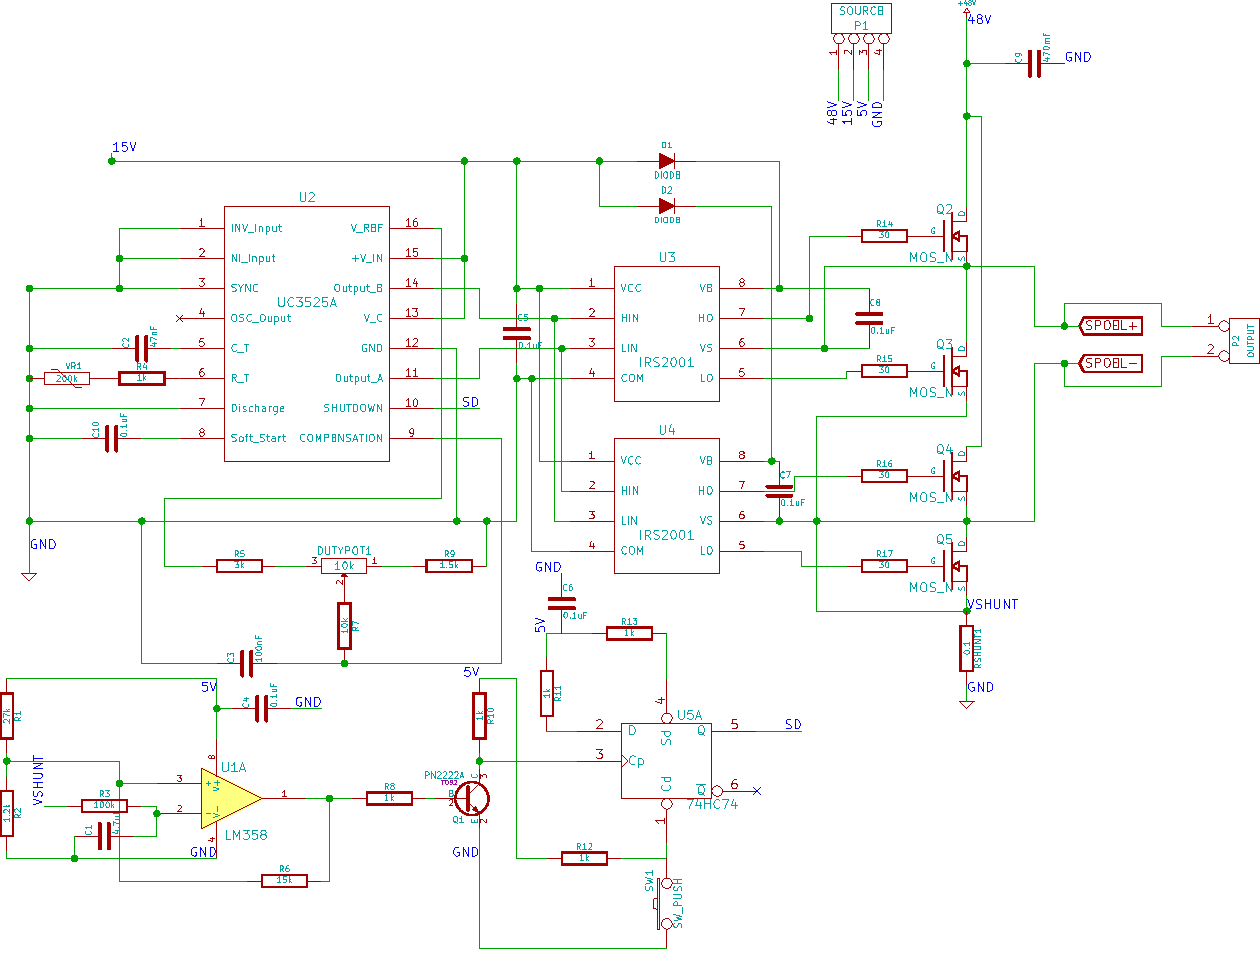
\includegraphics[width=\linewidth]{resources/DC-AC-rc.pdf}
	\caption{DC-AC subcircuit}
	\label{fig:DC-AC}
\end{figure}

\begin{figure}[h]
	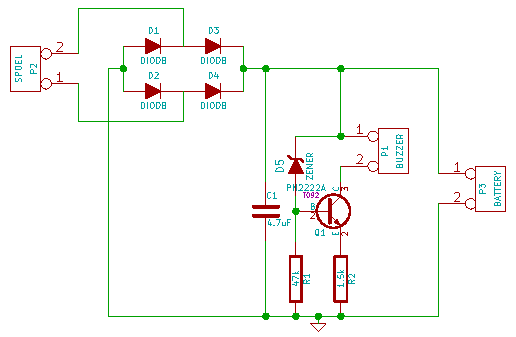
\includegraphics[width=\linewidth]{resources/AC-DC-rc.pdf}
	\caption{AC-DC subcircuit}
	\label{fig:AC-DC}
\end{figure}

\chapter{Invertor PCB}
\label{app:invertor-pcb}
\begin{figure}[h]
	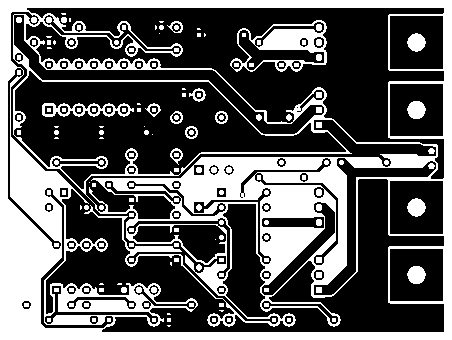
\includegraphics[width=\linewidth]{resources/DC-AC-F_Cu-rc.pdf}
	\caption{DC-AC PCB Front}
	\label{fig:DC-AC-PCB-Front}
\end{figure}

\begin{figure}[h]
	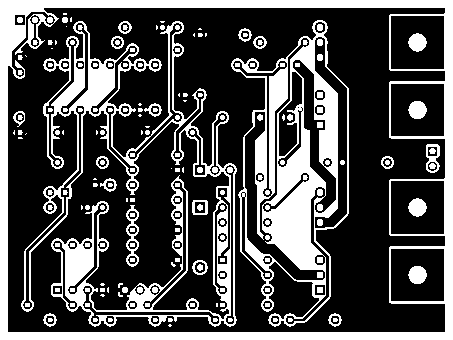
\includegraphics[width=\linewidth]{resources/DC-AC-B_Cu-rc.pdf}
	\caption{DC-AC PCB Back}
	\label{fig:DC-AC-PCB-Back}
\end{figure}

\chapter{GUI}
\label{app:gui}
\begin{figure}[h]
\centering
\begin{subfigure}[t]{0.49\linewidth}
	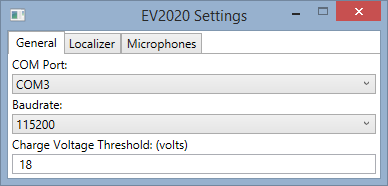
\includegraphics[width=\linewidth]{resources/UI-Settings-General.png}
	\caption{GUI Settings window, General tab}
	\label{fig:UI-Settings-General}
\end{subfigure}
\begin{subfigure}[t]{0.49\linewidth}
	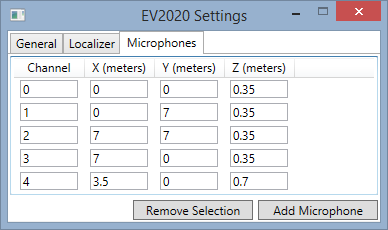
\includegraphics[width=\linewidth]{resources/UI-Settings-Microphones.png}
	\caption{GUI Settings window, Microphones tab}
	\label{fig:UI-Settings-Microphones}
\end{subfigure}
\begin{subfigure}[t]{0.48\linewidth}
	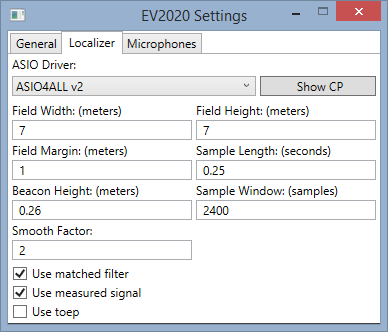
\includegraphics[width=\linewidth]{resources/UI-Settings-Localizer.png}
	\caption{GUI Settings window, Localizer tab}
	\label{fig:UI-Settings-Localizer}
\end{subfigure}

\caption{GUI Settings window, defined in SettingsWindow.xaml (Listing \ref{lst:Settings-SettingsWindow.xaml})}
\label{fig:UI-Settings}
\end{figure}

\begin{figure}[h]
\centering
	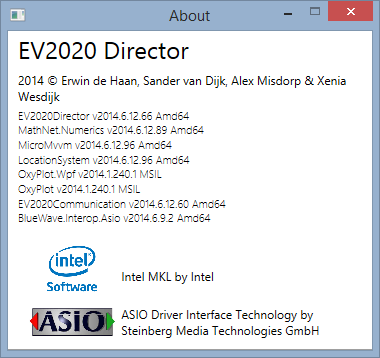
\includegraphics[width=0.7\linewidth]{resources/UI-About.png}
	\caption{GUI About window, defined in AboutWindow.xaml (Listing \ref{lst:Director-AboutWindow.xaml})}
	\label{fig:UI-About}
\end{figure}

\begin{figure}[h]
\centering
	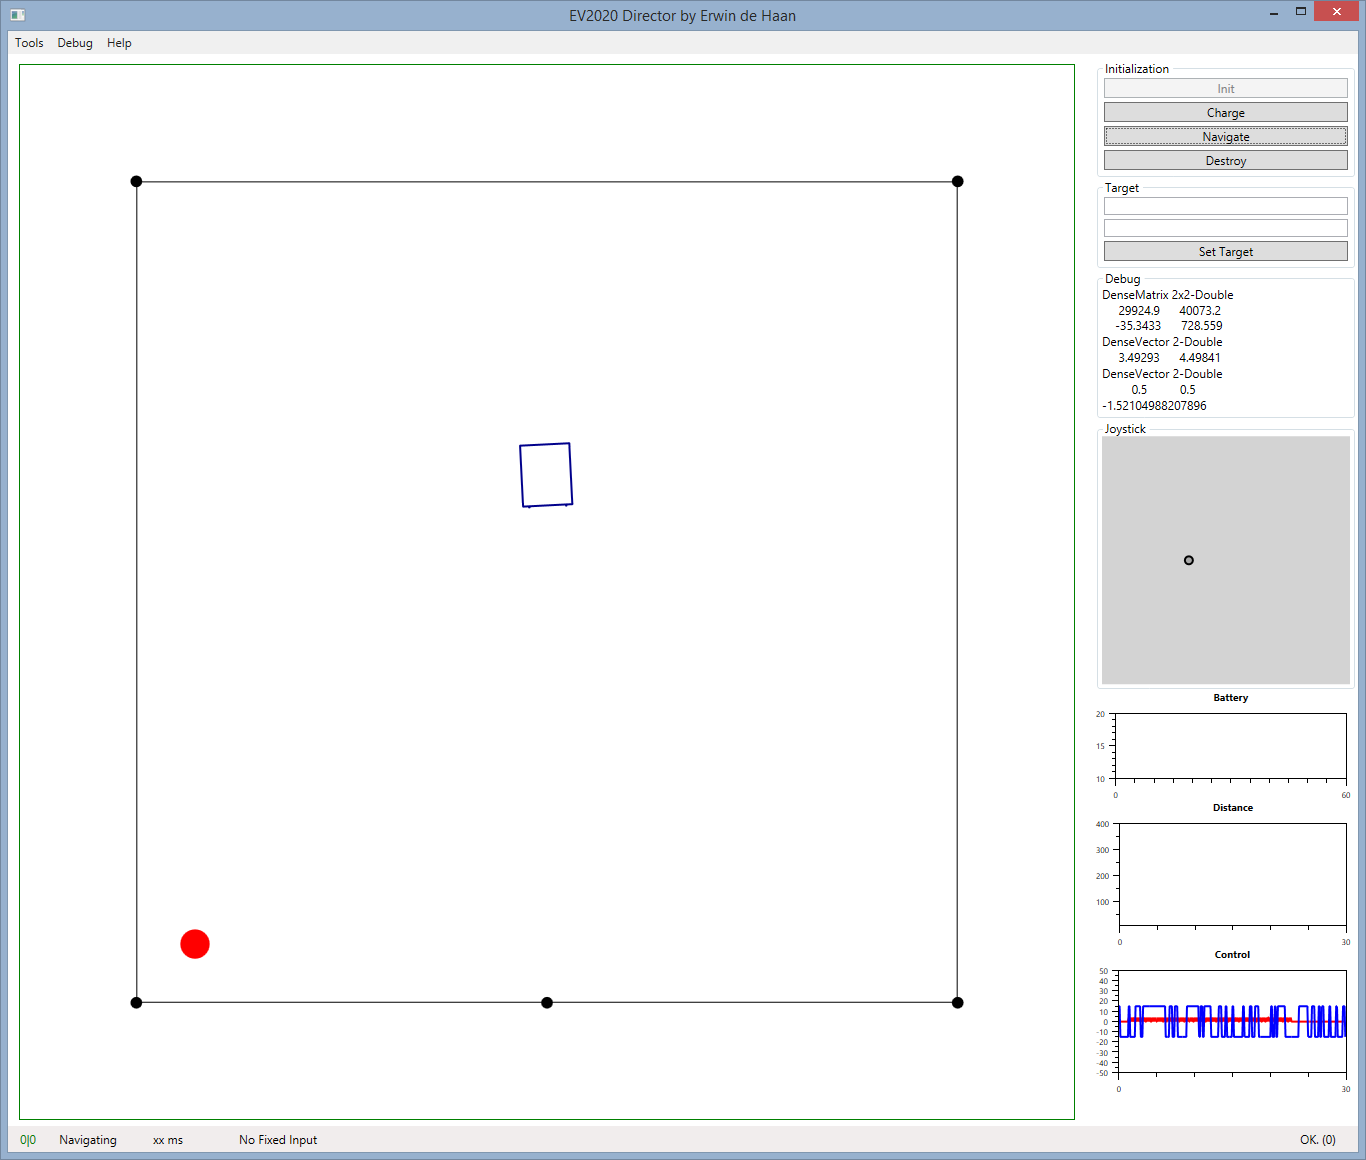
\includegraphics[width=\linewidth]{resources/UI-Main.png}
	\caption{GUI Main window, defined in MainWindow.xaml (Listing \ref{lst:Director-MainWindow.xaml}). No car was connected at the time so the graphs do not show any data and the trail is also not shown. The Car geometry (blue rectangle) also displays the actual sensor beam with the correct length and FOV when the sensor data is valid. The red dot is the target location. The black line is the filed boundary. The green line is the line beyond which a location is ``invalid''. The black dots are the microphones.}
	\label{fig:UI-Main}
\end{figure}

\chapter{Model}
\label{app:model}
\begin{figure}[H]
	\centering    	
    	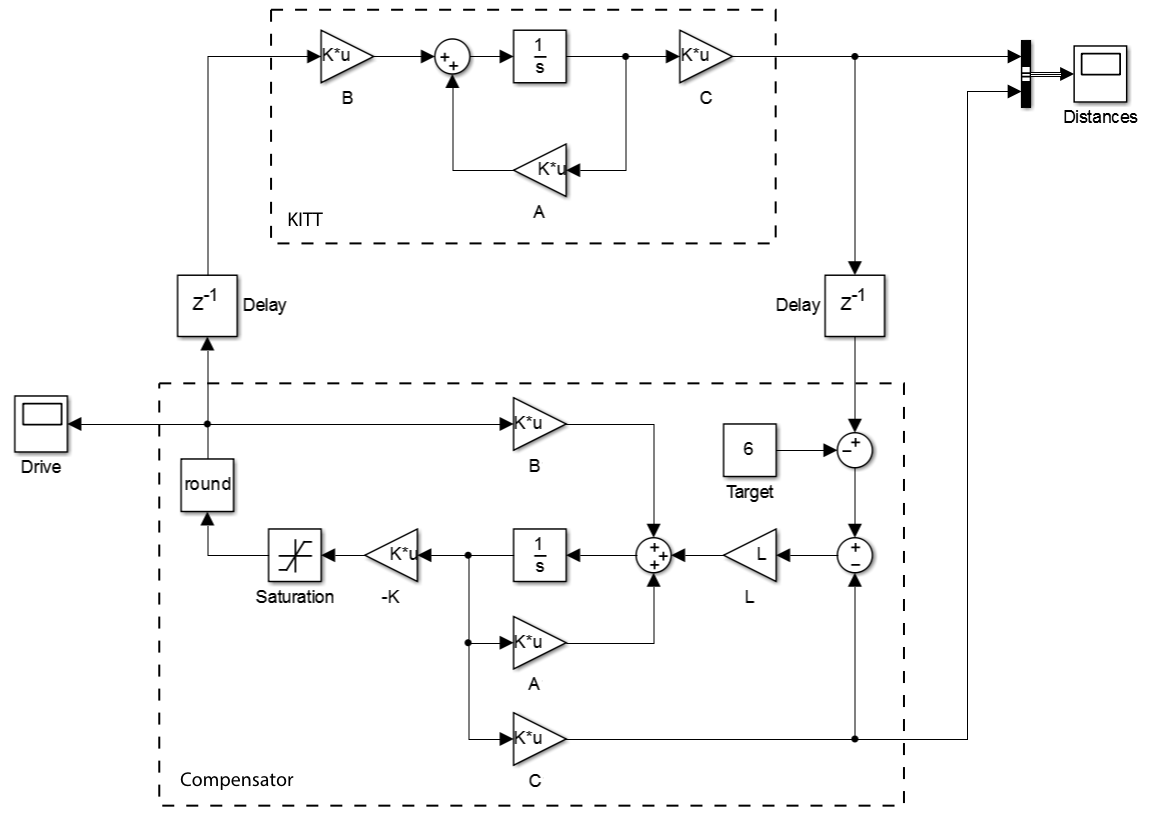
\includegraphics[width=\textwidth]{resources/model.png}
    	\caption{The model used to simulate the observer and controller}
    	\label{app:model}
\end{figure}

\chapter{Localization}
\label{app:localization}
\begin{figure}[H]
	\centering
	\setlength\figureheight{3cm}
    	\setlength\figurewidth{0.4\linewidth}
	% This file was created by matlab2tikz v0.4.6 running on MATLAB 8.2.
% Copyright (c) 2008--2014, Nico Schlömer <nico.schloemer@gmail.com>
% All rights reserved.
% Minimal pgfplots version: 1.3
% 
% The latest updates can be retrieved from
%   http://www.mathworks.com/matlabcentral/fileexchange/22022-matlab2tikz
% where you can also make suggestions and rate matlab2tikz.
% 
\begin{tikzpicture}

\begin{axis}[%
width=\figurewidth,
height=\figureheight,
scale only axis,
xmin=0,
xmax=0.8,
xlabel={Time (s)},
ymin=-0.005,
ymax=0.005,
ylabel={Response},
yticklabel style={/pgf/number format/fixed},
name=plot3
]
\addplot [color=blue,solid,forget plot]
  table[row sep=crcr]{
0	5.26905132574029e-05	\\
0.000479182639421314	0.000330209761159495	\\
0.00197923264108804	-0.000218391447560862	\\
0.00356261875395847	0.00059342390159145	\\
0.00395846528217607	-0.000262856512563303	\\
0.00454181806060202	-0.000788927194662392	\\
0.00570852361745392	-1.64508837769972e-05	\\
0.00693773125770859	-0.000678300915751606	\\
0.00781276042534751	-3.57627925495763e-07	\\
0.00908363612120404	-0.000290513067739084	\\
0.00989616320544018	0.00021970274974592	\\
0.0112712090403013	0.00046074396232143	\\
0.0118753958465282	0.000178694739588536	\\
0.012500416680556	-5.61475826543756e-05	\\
0.0132921097369912	0.000438809453044087	\\
0.0141463048768292	0.000136613860377111	\\
0.0157505250175006	-0.000631451664958149	\\
0.0158338611287043	-0.000574469624552876	\\
0.0166047201573386	-1.28746050904738e-05	\\
0.0180631021034034	-0.000403285084757954	\\
0.0197089902996767	0.000443697033915669	\\
0.0197923264108804	0.000335097342031077	\\
0.0217715590519684	-0.000110745444544591	\\
0.0220840694689823	-0.000464439450297505	\\
0.0231674389146305	-7.20024181646295e-05	\\
0.0246883229440981	0.000221729307668284	\\
0.0256050201673389	-0.000361800222890452	\\
0.0257508583619454	-0.000212430983083323	\\
0.0274592486416214	0.000812292215414345	\\
0.0277092569752325	0.000428795872721821	\\
0.0286676222540751	-0.000207066565053537	\\
0.0302301743391446	-0.000646710454020649	\\
0.0315010500350012	-1.28746050904738e-05	\\
0.0318135604520151	-0.000257134466664866	\\
0.0336052868428948	0.000226020842092112	\\
0.0350220007333578	-0.000241756468312815	\\
0.0355845194839828	0.000506043492350727	\\
0.0357095236507884	0.000540852604899555	\\
0.0375637521250708	-0.000293850927846506	\\
0.0387096236541218	8.67843700689264e-05	\\
0.0393763125437515	-0.000559687672648579	\\
0.0395846528217607	-0.000521183072123677	\\
0.0402513417113904	-5.24520946783014e-05	\\
0.0427722590753025	-0.000467181263957173	\\
0.0435222840761359	0.00056445604423061	\\
0.0443556451881729	0.000159621253260411	\\
0.0451265042168072	0.000672936497721821	\\
0.0455223507450248	0.000519156514201313	\\
0.0474807493583119	-0.000337004690663889	\\
0.0482307743591453	0.00035846236278303	\\
0.0490016333877796	-0.000367164670024067	\\
0.0506683556118537	-0.000424623547587544	\\
0.051439214640488	0.000144243254908361	\\
0.0523975799193306	-0.000264883070485666	\\
0.0531684389479649	0.000532150326762348	\\
0.0534184472815761	0.00020587447215803	\\
0.0543976465882196	-0.00075507175642997	\\
0.0558768625620854	0.000129818930872716	\\
0.056564385479516	-0.000275254278676584	\\
0.0574602486749558	-2.46763265749905e-05	\\
0.0593561452048402	0.00059950357535854	\\
0.0595228174272476	0.000758767244406044	\\
0.060835361178706	-0.000482440053019673	\\
0.0613353778459282	-4.01735342165921e-05	\\
0.0629812660422014	-0.000681161938700825	\\
0.0642729757658589	-1.08480462586158e-05	\\
0.0650438347944931	-0.000474929867777973	\\
0.0652730091003033	-0.000310421019094065	\\
0.0661688722957432	0.000483155308756977	\\
0.0677522584086136	0.000413775502238423	\\
0.0691481382712757	-0.000158548369654454	\\
0.0705023500783359	0.00015783311391715	\\
0.0711898729957665	-0.000498175679240376	\\
0.0712315410513684	-0.000499367772135884	\\
0.072481582719424	0.00064980989554897	\\
0.0741066368878963	4.52995336672757e-05	\\
0.0746274875829194	-0.000221848516957834	\\
0.0753566785559519	-0.000239133863942698	\\
0.0771275709190306	0.000109553351649083	\\
0.077585919530651	-0.000136852278956212	\\
0.0790651355045168	0.000343799620168284	\\
0.0803568452281743	0.000541091023478657	\\
0.0810860362012067	-8.11815334600396e-05	\\
0.0820860695356512	8.28504635137506e-05	\\
0.0829610987032901	-0.000325202970998362	\\
0.084127804260142	-0.000300049810903147	\\
0.0848569952331744	2.90870702883694e-05	\\
0.0860237007900263	-0.000536203442607075	\\
0.0868153938464615	7.02142788213678e-05	\\
0.0873987466248875	-0.000603199063334614	\\
0.0886487882929431	-0.000157594695338048	\\
0.0891904730157672	-0.000530719815287739	\\
0.0900238341278043	-0.000121593489893712	\\
0.0910030334344478	-0.000149726882227696	\\
0.0929614320477349	0.000460386334452778	\\
0.093211440381346	0.000544905720744282	\\
0.0938781292709757	0.000176787390955724	\\
0.0949614987166239	0.000203490286367014	\\
0.0967323910797027	-0.000332236319081858	\\
0.097503250108337	7.24792553228326e-05	\\
0.0987532917763925	-0.000494599400553852	\\
0.098899129970999	-0.000466585217509419	\\
0.099753325110837	0.000216960936086252	\\
0.101357545251508	-0.000286579161183909	\\
0.102649254975166	0.000360131292836741	\\
0.103336777892596	-2.12192553590285e-05	\\
0.103940964698823	0.00052773958304897	\\
0.105024334144471	0.000354528456227854	\\
0.10679522650755	-0.000183343916432932	\\
0.108253608453615	-2.57492101809476e-05	\\
0.108753625120837	-0.000269651442067698	\\
0.109628654288476	-0.00042867666343227	\\
0.110316177205907	0.000280976324575022	\\
0.110982866095537	-0.000263094931142405	\\
0.112337077902597	6.23464657110162e-05	\\
0.114107970265676	-0.000345706968801096	\\
0.114732991099703	7.58171154302545e-05	\\
0.115670522350745	-0.00018453600932844	\\
0.116628887629588	0.000449061451945454	\\
0.117483082769426	-0.000152945533045568	\\
0.118462282076069	0.000506997166667134	\\
0.11871229040968	0.000465393124613911	\\
0.120316510550352	-0.000311851530568674	\\
0.120816527217574	0.000197768240468577	\\
0.122379079302643	-0.000521183072123677	\\
0.123045768192273	-0.000154256835230626	\\
0.1236499549985	-0.000563740788493305	\\
0.124629154305144	-0.000514984189067036	\\
0.126045868195607	0.000161170974024571	\\
0.126629220974032	-6.75916744512506e-05	\\
0.127400080002667	0.000447988568339497	\\
0.129004300143338	0.000737786409445107	\\
0.130046001533384	4.88758159917779e-05	\\
0.131587719590653	0.000164985671290196	\\
0.132296076535885	-0.000234007864492014	\\
0.133525284176139	0.000158786788233556	\\
0.134504483482783	-0.000224113493459299	\\
0.134608653621787	-0.000293731718556955	\\
0.135650355011834	0.000212669401662424	\\
0.136504550151672	-0.000156879439600743	\\
0.137962932097737	0.000210285215871409	\\
0.140046334877829	0.000168442740687169	\\
0.140400513350445	-9.50098183238879e-05	\\
0.14073385779526	-0.000275135069387034	\\
0.141754725157505	0.000155568137415685	\\
0.143254775159172	2.21729296754347e-05	\\
0.143858961965399	-0.00019073489238508	\\
0.144879829327644	-0.000112652793177404	\\
0.145650688356279	8.82148815435357e-05	\\
0.147296576552552	-0.000135183348902501	\\
0.147984099469982	0.000121116652735509	\\
0.148775792526418	-9.84668877208605e-05	\\
0.149588319610654	0.000175356879481114	\\
0.15221340711357	0.000913500902242959	\\
0.152296743224774	-0.000495553074870259	\\
0.152796759891996	0.00141692173201591	\\
0.153942631421047	-0.00153529667295516	\\
0.155984366145538	0.00145936023909599	\\
0.15625520850695	-0.00128006946761161	\\
0.157755258508617	-0.00250041508115828	\\
0.158213607120237	0.00165843986906111	\\
0.158380279342645	0.00182783626951277	\\
0.158776125870862	-0.00296628521755338	\\
0.160838694623154	-0.00167381786741316	\\
0.16119287309577	0.00213122391141951	\\
0.163109603653455	-0.00133764755446464	\\
0.163463782126071	0.00087249290663749	\\
0.164817993933131	0.000598549901042134	\\
0.165172172405747	-0.000492572842631489	\\
0.166859728657622	0.000265836744802073	\\
0.167505583519451	-0.00103509437758476	\\
0.169255641854728	-0.000815034029074013	\\
0.169755658521951	0.000306487112538889	\\
0.171109870329011	-0.000662684498820454	\\
0.171797393246442	0.000246167212026194	\\
0.172151571719057	-0.000362992315785959	\\
0.17333911130371	0.000833511468954384	\\
0.174089136304543	0.000222325354116037	\\
0.174526650888363	-0.000278234510915354	\\
0.177464248808294	0.000301718740956858	\\
0.178026767558919	-0.000327825575368479	\\
0.178401780059335	0.000719785748515278	\\
0.178985132837761	-0.000528574048075825	\\
0.180839361312044	-0.000662326870951802	\\
0.181589386312877	0.000332951574819162	\\
0.183151938397947	0.000325202970998362	\\
0.183735291176373	-0.000655531941447407	\\
0.185089502983433	0.00123298179823905	\\
0.185339511317044	-0.000846028444357216	\\
0.186339544651488	0.00125980388838798	\\
0.187860428680956	-0.000300765066640452	\\
0.189006300210007	0.000952005502767861	\\
0.189318810627021	-0.000651240407023579	\\
0.189922997433248	0.000737547990866005	\\
0.190298009933664	-0.00114583980757743	\\
0.192985599519984	0.000435590802226216	\\
0.193527284242808	-0.000922799226827919	\\
0.195069002300077	-0.000479459820780903	\\
0.19536067868929	0.000640392361674458	\\
0.196839894663155	-0.00049269205192104	\\
0.197652421747392	0.00107514869887382	\\
0.198485782859429	0.00105810177046806	\\
0.199027467582253	-0.000670671521220356	\\
0.201027534251142	0.000927567598409951	\\
0.201465048834961	-0.00111925613600761	\\
0.202402580086003	-0.00112164032179862	\\
0.202860928697623	0.000751137849874794	\\
0.20390263008767	0.000748276826925576	\\
0.205402680089336	-0.00130236160475761	\\
0.20615270509017	0.000751733896322548	\\
0.207652755091836	-0.00092899810988456	\\
0.207861095369846	-0.0010114909382537	\\
0.209361145371512	0.00032031539012678	\\
0.210465348844961	0.000877976533956826	\\
0.21088202940098	-0.000496745167765766	\\
0.211694556485216	0.000789642450399697	\\
0.213069602320077	-0.000680089055094868	\\
0.213652955098503	0.000733375665731728	\\
0.21448631621054	-0.000896096345968544	\\
0.215923864128804	-0.00115716469008476	\\
0.217423914130471	0.000515341816935688	\\
0.218486449548318	-0.00086188327986747	\\
0.219486482882763	0.000963330385275185	\\
0.220028167605587	-0.00102043163497001	\\
0.22077819260642	0.00107491028029472	\\
0.22213240441348	0.000717282353434712	\\
0.223507450248342	-0.000617981015238911	\\
0.223611620387346	-0.000852465745992959	\\
0.224069968998967	0.00111997139174491	\\
0.226695056501883	-0.000907421228475869	\\
0.227257575252508	0.000772953149862587	\\
0.228049268308944	-0.000603914319071919	\\
0.229299309976999	0.000885963556356728	\\
0.229965998866629	-0.000682830868754536	\\
0.230841028034268	0.000704526959452778	\\
0.231695223174106	0.00106787693221122	\\
0.233111937064569	-0.000895023462362587	\\
0.23471615720524	0.000799894449301064	\\
0.235174505816861	-0.000734448549337685	\\
0.23538284609487	-0.000410795269999653	\\
0.23561202040068	0.000970840570516884	\\
0.238507950265009	-0.000873208162374794	\\
0.239091303043435	0.000399112759623677	\\
0.240299676655889	-0.000756740686483681	\\
0.240945531517717	0.00039350992301479	\\
0.242716423880796	-0.00059807306388393	\\
0.243070602353412	0.000982761499471962	\\
0.243508116937231	0.00122189533431083	\\
0.244883162772092	-0.000268220930593088	\\
0.245529017633921	0.000680565892253071	\\
0.247195739857995	-0.00054764753440395	\\
0.248299943331444	-0.000907540437765419	\\
0.24888329610987	0.000346779852407053	\\
0.250800026667556	-0.000922680017538369	\\
0.251029200973366	0.000424981175456196	\\
0.251904230141005	-0.00105929386336356	\\
0.252570919030634	0.000735402223654091	\\
0.253883462782093	-0.000768661615438759	\\
0.254237641254708	0.000882148859091103	\\
0.255362678755959	0.000917911645956337	\\
0.256112703756792	-0.000692486821208149	\\
0.257946098203273	0.000945568201132119	\\
0.258383612787093	-0.000662207661662251	\\
0.259758658621954	0.00052928930381313	\\
0.260404513483783	-0.000759840128012002	\\
0.261487882929431	-0.000696301518473774	\\
0.262300410013667	0.000241994886891916	\\
0.263737957931931	0.000425815640483052	\\
0.263987966265542	-0.000497102795634419	\\
0.265779692656422	0.00041341787436977	\\
0.266321377379246	-0.000568270741496235	\\
0.267946431547718	0.000699877797160298	\\
0.268238107936931	-0.00017166139150504	\\
0.270175672522417	0.000584721623454243	\\
0.270738191273042	-0.000418543873820454	\\
0.271029867662255	0.000522613583598286	\\
0.272904930164339	-0.000564694462809712	\\
0.272988266275543	-0.000896453973837197	\\
0.273800793359779	0.000198960333364084	\\
0.275259175305844	-0.000769138452596962	\\
0.276905063502117	0.000467896519694477	\\
0.277363412113737	-0.000413894711527973	\\
0.27811343711457	0.000738620874471962	\\
0.279030134337811	0.000845313188619912	\\
0.28080102670089	-0.000106096282252111	\\
0.281384379479316	0.000426292477641255	\\
0.282676089202973	-0.000653982220683247	\\
0.283634454481816	0.000345468550221995	\\
0.284301143371446	-0.000286579161183909	\\
0.285051168372279	-0.000640869198832661	\\
0.285801193373112	0.000597477017436177	\\
0.287384579485983	-0.000348687201039866	\\
0.287822094069802	0.000413894711527973	\\
0.289259641988066	-0.000461459218058735	\\
0.289905496849895	0.000454068242106587	\\
0.291051368378946	0.00047135358909145	\\
0.291613887129571	-0.000570297299418598	\\
0.292926430881029	0.00043165689567104	\\
0.294613987132904	-0.000705123005900532	\\
0.295259841994733	0.000105857863673009	\\
0.296447381579386	-0.000920176622457802	\\
0.297155738524617	-0.000720858632121235	\\
0.298364112137071	0.000316500692861155	\\
0.2990099669989	-0.000602006970439106	\\
0.300260008666956	0.000684142170939595	\\
0.301468382279409	0.000169754042872228	\\
0.302239241308044	0.000703573285136372	\\
0.302718423947465	0.000703573285136372	\\
0.303885129504317	-0.000359296827809885	\\
0.304718490616354	0.000322937994496897	\\
0.305968532284409	-0.000442862568888813	\\
0.30709356978566	3.79085577151272e-05	\\
0.307676922564085	-0.000528216420207173	\\
0.309426980899363	0.000273346930043772	\\
0.310302010067002	-0.000553846417460591	\\
0.311177039234641	-0.000364422827260569	\\
0.3124895829861	0.000231027632253245	\\
0.313218773959132	-0.000195503263967112	\\
0.313885462848762	0.000487208424601704	\\
0.315156338544618	-0.000125408187159337	\\
0.316448048268276	0.000669837056193501	\\
0.316468882296077	0.000626087246928364	\\
0.318156438547952	-0.000480413495097309	\\
0.31901063368779	-0.000655293522868305	\\
0.319489816327211	0.000106453910120763	\\
0.320510683689456	-0.000294923811452463	\\
0.321927397579919	0.000234484701650217	\\
0.322489916330544	-0.000163793578394689	\\
0.324114970499017	0.000632047711405903	\\
0.325573352445082	-7.90357662481256e-05	\\
0.325740024667489	0.000591754971537739	\\
0.326365045501517	0.000403046666178852	\\
0.326740058001933	-0.000183820753591135	\\
0.328635954531818	0.000416278897318989	\\
0.330302676755892	-0.00039196020225063	\\
0.331073535784526	5.94854427617975e-05	\\
0.332031901063369	-0.000432372151408345	\\
0.332615253841795	-0.000607729016337544	\\
0.334031967732258	0.00018084050680045	\\
0.335282009400313	-0.000437378941569477	\\
0.335948698289943	0.000522255955729634	\\
0.336636221207374	0.000555038510356098	\\
0.338157105236841	-0.000126123442896642	\\
0.338594619820661	0.000455260335002095	\\
0.339073802460082	-0.000366926251444966	\\
0.340969698989966	0.000270485907094553	\\
0.342115570519017	-0.000281453161733225	\\
0.342490583019434	8.52346493047662e-05	\\
0.344073969132304	-0.000481486378703266	\\
0.345657355245175	2.98023269351688e-06	\\
0.346115703856795	-0.000380754529032856	\\
0.346136537884596	-0.000324368505971506	\\
0.347761592053068	0.000425338803324848	\\
0.348553285109504	0.000679850636515766	\\
0.349115803860129	0.000149726882227696	\\
0.350095003166772	0.000435471592936665	\\
0.351678389279643	-0.00025177004863508	\\
0.352136737891263	0.000177979483851232	\\
0.354053468448948	-0.000612855015788227	\\
0.354136804560152	-0.000708103238139302	\\
0.355928530951032	-0.000130176558741368	\\
0.356178539284643	-0.000562310277018696	\\
0.357761925397513	0.00031876566936262	\\
0.358241108036935	-0.000161290183314122	\\
0.35880362678756	0.000490665493998677	\\
0.361782892763092	0.000315070181386545	\\
0.3619495649855	-0.000106811537989415	\\
0.36286626220874	-0.0003386736207176	\\
0.363574619153972	0.000187516241567209	\\
0.365449681656055	-0.000449538289103657	\\
0.365803860128671	9.78708412731066e-05	\\
0.36622054068469	0.000162839904078282	\\
0.367303910130338	-0.000409007130656391	\\
0.368220607353578	-0.000533819256816059	\\
0.368699789993	-2.28881872317288e-05	\\
0.370241508050268	-0.000159502043970861	\\
0.371512383746125	0.000630497990641743	\\
0.371949898329944	-4.76837215046544e-07	\\
0.373783292776426	0.000416278897318989	\\
0.37386662888763	0.000268816977040842	\\
0.375470849028301	-0.000267386465566233	\\
0.375825027500917	-8.32080913824029e-05	\\
0.37703340111337	-0.000807643053121865	\\
0.37813760458682	-0.000515222607646137	\\
0.378387612920431	-3.45706976077054e-05	\\
0.379887662922097	-0.000322937994496897	\\
0.381700223340778	0.000297188787953928	\\
0.381866895563185	0.000216245680348948	\\
0.382908596953232	0.000904917833395302	\\
0.384804493483116	0.000590205250773579	\\
0.385367012233741	0.000192403822438791	\\
0.385721190706357	0.00025784972240217	\\
0.387471249041635	-0.000308990507619455	\\
0.38780459348645	1.62124651978957e-05	\\
0.388762958765292	-0.000670790730509907	\\
0.389971332377746	-7.25984646123834e-05	\\
0.391450548351612	-0.000464439450297505	\\
0.391617220574019	-0.000283360510366037	\\
0.392721424047468	0.000136375441798009	\\
0.393721457381913	-0.000203013449208811	\\
0.39455481849395	0.000289440184133127	\\
0.3956798559952	-0.000116109862574376	\\
0.396221540718024	0.000398755131755024	\\
0.398659121970732	0.000434637127909809	\\
0.399304976832561	6.27040935796686e-05	\\
0.399554985166172	0.000322580366628245	\\
0.401159205306844	-0.000461101590190083	\\
0.402096736557885	-0.00050187116721645	\\
0.403159271975733	-6.69956280034967e-05	\\
0.403742624754158	-0.000303030043141916	\\
0.405326010867029	0.000482916890177876	\\
0.405992699756659	0.000207662611501291	\\
0.406659388646288	0.000653147755656391	\\
0.408096936564552	0.000548005162272602	\\
0.40938864628821	-0.000113725676783361	\\
0.409596986566219	-6.27040935796686e-05	\\
0.411326210873696	-0.00062239175895229	\\
0.412263742124737	-0.000619649945292622	\\
0.412930431014367	-0.000177979483851232	\\
0.414284642821427	-0.000716805516276509	\\
0.415368012267076	-3.86238134524319e-05	\\
0.416430547684923	-0.000233769445912912	\\
0.417076402546752	0.000203967123525217	\\
0.418222274075803	0.000326871901052073	\\
0.418534784492816	-0.000115752234705724	\\
0.419472315743858	-8.57114864629693e-05	\\
0.420076502550085	0.000421285687480122	\\
0.421493216440548	0.000247836142079905	\\
0.422472415747192	-0.000140905394800939	\\
0.423347444914831	-1.71661395143019e-05	\\
0.424347478249275	-0.000340342550771311	\\
0.425951698389946	-0.000385284482035786	\\
0.427118403946798	-1.26361865113722e-05	\\
0.427264242141405	-0.000128984465845861	\\
0.429097636587886	0.000352740316884592	\\
0.429243474782493	0.000315189390676096	\\
0.429701823394113	1.08480462586158e-05	\\
0.432681089369646	0.000180006041773595	\\
0.432951931731058	-0.000114321723231114	\\
0.433389446314877	-5.36441848453251e-06	\\
0.435139504650155	-0.000270247488515452	\\
0.435285342844762	-0.000365018873708323	\\
0.436577052568419	2.34842336794827e-05	\\
0.437931264375479	-0.000345230131642893	\\
0.438952131737725	2.15768832276808e-05	\\
0.439181306043535	-0.000231742887990549	\\
0.440993866462215	0.000522613583598286	\\
0.441514717157239	0.000710725842509419	\\
0.442285576185873	0.000406980572734028	\\
0.443743958131938	0.000652194081339985	\\
0.444973165772192	9.11951137823053e-05	\\
0.445306510217007	0.000269770651357248	\\
0.446764892163072	-0.000245094328420237	\\
0.447681589386313	-0.000383615551982075	\\
0.448931631054368	3.65972555300687e-05	\\
0.449098303276776	-0.000136852278956212	\\
0.450473349111637	0.000135302558192052	\\
0.451494216473882	-4.98294903081842e-05	\\
0.452265075502517	0.000266790419118479	\\
0.453515117170572	-5.84125609748298e-06	\\
0.454515150505017	0.000286936789052561	\\
0.455452681756059	0.000187397032277659	\\
0.45682772759092	-0.000133872046717443	\\
0.457473582452748	0.000192999868886545	\\
0.458869462315411	-0.000387549458537251	\\
0.459098636621221	-0.000499486981425434	\\
0.459681989399647	-0.000195145636098459	\\
0.460994533151105	-0.000377774296794087	\\
0.462744591486383	0.000148415580042638	\\
0.46291126370879	-3.21865127261844e-06	\\
0.464202973432448	0.000523805676493794	\\
0.465078002600087	0.000631094037089497	\\
0.465703023434114	0.000198483496205881	\\
0.466828060935365	0.000324010878102854	\\
0.467828094269809	-0.000111937537440099	\\
0.46897396579886	9.05990673345514e-05	\\
0.470036501216707	-0.000238776236074045	\\
0.470744858161939	-3.39746511599515e-05	\\
0.472536584552818	-0.000473260937724262	\\
0.472765758858629	-0.000360965757863596	\\
0.47459915330511	2.74181402346585e-05	\\
0.474932497749925	-0.000201106100575998	\\
0.476640888029601	0.000265955954091623	\\
0.477140904696823	0.000522732792887837	\\
0.478557618587286	0.00012123586202506	\\
0.479036801226708	0.00035846236278303	\\
0.480557685256175	-9.79900505626574e-05	\\
0.480641021367379	-4.22000921389554e-05	\\
0.481328544284809	-0.000329971342580393	\\
0.483182772759092	-0.000298142462270334	\\
0.484516150538351	1.9311906726216e-05	\\
0.484870329010967	-0.000153541579493321	\\
0.486432881096037	0.000229239492909983	\\
0.48695373179106	-4.29153487857548e-06	\\
0.488328777625921	0.000366926251444966	\\
0.488641288042935	0.000382304249797016	\\
0.489474649154972	0.000159502043970861	\\
0.490662188739625	0.00035238268901594	\\
0.492308076935898	-4.22000921389554e-05	\\
0.492558085269509	9.09566952032037e-05	\\
0.494391479715991	-0.000424385129008442	\\
0.49549568318944	-0.000258803396718577	\\
0.496204040134671	-0.000513672886881977	\\
0.496891563052102	-0.000421881733927876	\\
0.497995766525551	-4.49419057986233e-05	\\
0.49843328110937	-0.000169873252161779	\\
0.500287509583653	0.00044238573173061	\\
0.500725024167472	0.000372648297343403	\\
0.50201673389113	0.000120639815577306	\\
0.502766758891963	0.000338792830007151	\\
0.504120970699023	-6.00814892095514e-05	\\
0.50449598319944	4.29153478762601e-05	\\
0.505579352645088	-0.000201821356313303	\\
0.506558551951732	2.95639074465726e-05	\\
0.507433581119371	-0.000163078322657384	\\
0.50853778459282	-8.17775799077936e-05	\\
0.509933664455482	0.00024247172405012	\\
0.510433681122704	0.000172972693690099	\\
0.512183739457982	0.000464558659587055	\\
0.512267075569186	0.000377774296794087	\\
0.514100470015667	9.32216789806262e-05	\\
0.514246308210274	0.000187039404409006	\\
0.516225540851362	-0.000245213537709787	\\
0.516767225574186	-0.00014412404561881	\\
0.517829760992033	-0.000389814435038716	\\
0.518933964465482	-0.000219106703298166	\\
0.519975665855529	6.16312099737115e-05	\\
0.520288176272542	-8.84533001226373e-05	\\
0.521975732524418	0.000336408644216135	\\
0.523121604053468	7.25984646123834e-05	\\
0.5238299609987	0.000366687832865864	\\
0.524767492249742	0.000317215948598459	\\
0.525600853361779	4.22000921389554e-05	\\
0.526684222807427	0.000312089949147776	\\
0.527934264475483	-9.29832604015246e-05	\\
0.52810093669789	2.47955358645413e-05	\\
0.528350945031501	-0.000292420416371897	\\
0.530455181839395	-0.000313162832753733	\\
0.531351045034835	6.92606045049615e-05	\\
0.532184406146872	-6.85453487676568e-05	\\
0.53395529850995	0.000385046063456684	\\
0.534413647121571	0.000500202237162739	\\
0.53574702490083	0.00020289423991926	\\
0.536122037401247	0.000304102926747873	\\
0.53776792559752	-5.44786526006646e-05	\\
0.537976265875529	1.77621859620558e-05	\\
0.539809660322011	-0.000447154103312641	\\
0.540059668655622	-0.00026690962840803	\\
0.541893063102103	-0.000545620976481587	\\
0.541934731157705	-0.000513315259013325	\\
0.543851461715391	-0.000223159819142893	\\
0.544184806160205	-0.00028824809123762	\\
0.54585152838428	6.83069301885553e-05	\\
0.545997366578886	0.000148415580042638	\\
0.547039067968932	-0.000120162978419103	\\
0.548205773525784	0.000163435950526036	\\
0.54945581519384	-8.83340908330865e-05	\\
0.550664188806294	0.000136375441798009	\\
0.551226707556919	-0.000211477308766916	\\
0.552330911030368	-0.000277876883046702	\\
0.552851761725391	-0.000101208701380529	\\
0.555372679089303	-0.000230670004384592	\\
0.555643521450715	7.34329296392389e-05	\\
0.556226874229141	-0.000196337728993967	\\
0.556935231174372	0.0001274347450817	\\
0.558560285342845	0.000251054792897776	\\
0.558810293676456	4.68492580694146e-05	\\
0.560497849928331	0.000171184554346837	\\
0.561497883262775	-4.94718624395318e-05	\\
0.562185406180206	0.000126361861475743	\\
0.563352111737058	-0.000255107908742502	\\
0.563831294376479	-0.000283360510366037	\\
0.564164638821294	-9.76324226940051e-05	\\
0.565789692989766	-0.000185012846486643	\\
0.567185572852428	0.000235676794545725	\\
0.567852261742058	5.65052105230279e-05	\\
0.568852295076503	0.000320673017995432	\\
0.570185672855762	0.000516891537699848	\\
0.570977365912197	0.000145196929224767	\\
0.571602386746225	0.000197768240468577	\\
0.573581619387313	-0.000173687949427404	\\
0.573852461748725	-4.81605602544732e-05	\\
0.57464415480516	-0.000245213537709787	\\
0.575560852028401	-0.000209689169423655	\\
0.576644221474049	6.19888396613533e-06	\\
0.577623420780693	-5.4836280469317e-05	\\
0.578998466615554	0.000166296973475255	\\
0.579602653421781	-5.57899547857232e-05	\\
0.580790193006434	0.000183701544301584	\\
0.5822902430081	0.000182747855433263	\\
0.582936097869929	-0.000109791770228185	\\
0.583894463148772	8.20159984868951e-05	\\
0.585394513150438	-0.000243544607656077	\\
0.586207040234675	-0.000100374236353673	\\
0.586602886762892	-0.000345587759511545	\\
0.588561285376179	-0.000377178250346333	\\
0.589269642321411	-6.66380001348443e-05	\\
0.590123837461249	-0.000226616888539866	\\
0.590790526350878	3.38554418704007e-05	\\
0.59172805760192	-7.36713482183404e-05	\\
0.592019733991133	0.00016558171773795	\\
0.593728124270809	7.86781401984626e-06	\\
0.594936497883263	0.000298380880849436	\\
0.596019867328911	0.000244736700551584	\\
0.597019900663355	-7.82013012212701e-05	\\
0.597311577052568	1.26361865113722e-05	\\
0.599269975665855	-0.000467538891825825	\\
0.599290809693656	-0.00046527391532436	\\
0.601270042334744	-0.000245213537709787	\\
0.60139504650155	-0.000363349943654612	\\
0.603249274975832	0.000207185774343088	\\
0.603499283309444	0.000132918372401036	\\
0.605228507616921	0.000478744565043598	\\
0.605291009700323	0.00050652032950893	\\
0.607186906230208	0.000241398840444162	\\
0.607207740258009	0.000259995489614084	\\
0.609166138871296	-4.52995345767704e-06	\\
0.609353645121504	0.000129342093714513	\\
0.611166205540185	-0.000126123442896642	\\
0.61129120970699	1.31130236695753e-05	\\
0.612166238874629	-0.000249505072133616	\\
0.61331211040368	-0.000221610098378733	\\
0.614728824294143	2.98023260256741e-05	\\
0.615603853461782	-0.000145554557093419	\\
0.617041401380046	0.000258088140981272	\\
0.617270575685856	0.000383257924113423	\\
0.618999799993333	0.000118613257654943	\\
0.619208140271342	0.000283479719655588	\\
0.62072902430081	-0.000213861494557932	\\
0.621749891663055	-0.000332713156240061	\\
0.622166572219074	-8.55922771734186e-05	\\
0.625	-0.000311613111989573	\\
};
\addplot [color=red,mark size=1.7pt,only marks,mark=*,mark options={solid},forget plot]
  table[row sep=crcr]{
0.155	0	\\
};
\end{axis}

\begin{axis}[%
width=\figurewidth,
height=\figureheight,
scale only axis,
xmin=0,
xmax=0.8,
xlabel={Time (s)},
ymin=-0.001,
ymax=0.001,
ylabel={Response},
yticklabel style={/pgf/number format/fixed},
name=plot1,
at=(plot3.above north west),
anchor=below south west
]
\addplot [color=blue,solid,forget plot]
  table[row sep=crcr]{
0	2.6583675207803e-05	\\
0.00129170972365746	0.000192284613149241	\\
0.00197923264108804	-2.12192553590285e-05	\\
0.00283342778092603	0.000181078925379552	\\
0.00395846528217607	-5.56707454961725e-05	\\
0.00533351111703723	-0.00018906596233137	\\
0.00593769792326411	1.47819537232863e-05	\\
0.0060835361178706	9.94205620372668e-05	\\
0.00747941598053268	-0.000192523031728342	\\
0.00818777292576419	-0.000188827543752268	\\
0.00968782292743091	0.000106215491541661	\\
0.0102711757058569	-0.000179052367457189	\\
0.011667055568519	0.000374794064555317	\\
0.0118753958465282	0.000264167814748362	\\
0.0126670889029634	-0.000107765212305821	\\
0.0149588319610654	0.000178933158167638	\\
0.0158338611287043	-0.000146031394251622	\\
0.0158755291843061	-0.000168442740687169	\\
0.0167922264075469	0.000115990653284825	\\
0.0190839694656489	-0.000219941168325022	\\
0.0197923264108804	0.000213384657399729	\\
0.0200423347444915	0.000271677999990061	\\
0.021021534051135	-0.000277757673757151	\\
0.0221465715523851	0.000124692931422032	\\
0.0237299576652555	-0.000121355071314611	\\
0.0240216340544685	-0.000132322325953282	\\
0.0252716757225241	0.00027608874370344	\\
0.0267508916963899	-5.91278148931451e-05	\\
0.0277092569752325	0.000122070327051915	\\
0.0283967798926631	0.000184059172170237	\\
0.0292093069768992	-0.000181078925379552	\\
0.0304801826727558	-0.000229358702199534	\\
0.0316468882296077	4.94718624395318e-05	\\
0.0321677389246308	-0.000256776838796213	\\
0.0330636021200707	8.20159984868951e-05	\\
0.0343136437881263	-0.000171542182215489	\\
0.0351678389279643	0.000117182746180333	\\
0.0356470215673856	-1.69277209352003e-05	\\
0.0372929097636588	0.000150084510096349	\\
0.0381262708756959	0.000172734275110997	\\
0.0387721257375246	-9.36985161388293e-05	\\
0.0408138604620154	-0.000278592138784006	\\
0.0415222174072469	6.42538143438287e-05	\\
0.0415847194906497	6.61611629766412e-05	\\
0.0429805993533118	-0.000401258526835591	\\
0.0435222840761359	-0.000171899810084142	\\
0.0442514750491683	0.000138759627589025	\\
0.0458973632454415	0.0003234148316551	\\
0.0473349111637055	-9.21487953746691e-05	\\
0.0474807493583119	-9.19103767955676e-05	\\
0.0487932931097703	2.77757681033108e-05	\\
0.0496266542218074	-0.000142812743433751	\\
0.050876695889863	9.08374859136529e-05	\\
0.0520642354745158	8.88109279912896e-05	\\
0.0531059368645622	-0.000101327910670079	\\
0.054293476449215	0.000189542799489573	\\
0.0552726757558585	-0.00027608874370344	\\
0.0556060202006734	-0.000260949163930491	\\
0.0571685722857429	6.79493041388923e-06	\\
0.0584394479815994	0.000143647208460607	\\
0.0593353111770392	-6.42538143438287e-05	\\
0.0593561452048402	-5.98430706304498e-05	\\
0.0601686722890763	0.000126361861475743	\\
0.0616478882629421	1.1682512194966e-05	\\
0.0627520917363912	8.97646023076959e-05	\\
0.0632937764592153	6.5207488660235e-05	\\
0.0651896729890996	-0.000210046797292307	\\
0.0658355278509284	-0.000237584143178537	\\
0.0666480549351645	3.4213069739053e-05	\\
0.0676897563252108	-0.000200390844838694	\\
0.0692314743824794	2.19345110963332e-05	\\
0.0701065035501183	-7.1167953137774e-05	\\
0.0711690389679656	0.000382542668376118	\\
0.0712107070235675	0.00037682062247768	\\
0.0725857528584286	-0.000195741682546213	\\
0.0744816493883129	8.77380443853326e-05	\\
0.0751691723057435	-0.000180125251063146	\\
0.0752941764725491	-0.000208258657949045	\\
0.0765025500850028	6.10351635259576e-05	\\
0.0776484216140538	0.000168323531397618	\\
0.0788359611987066	-7.05719066900201e-05	\\
0.07958598619954	0.000157237067469396	\\
0.0804610153671789	-0.000132322325953282	\\
0.0816068868962299	-6.59227443975396e-05	\\
0.0827944264808827	0.000111460700281896	\\
0.0843986466215541	-2.40802801272366e-05	\\
0.0848778292609754	0.000178813948878087	\\
0.0851278375945865	0.000126600280054845	\\
0.0864195473182439	-0.000151038184412755	\\
0.0880029334311144	0.000220418005483225	\\
0.0890029667655589	-0.000151395812281407	\\
0.0893988132937765	-0.000236630468862131	\\
0.0903571785726191	0.000142097487696446	\\
0.0918780626020867	4.55379522463772e-05	\\
0.092669755658522	-0.000151991858729161	\\
0.0930447681589386	-0.000158667578944005	\\
0.0943156438547952	0.000125765815027989	\\
0.0950031667722257	-3.34978140017483e-05	\\
0.0964823827460915	0.000248193769948557	\\
0.096919897329911	0.000155687346705236	\\
0.0976699223307444	-8.21352077764459e-05	\\
0.098899129970999	-5.43594433111139e-05	\\
0.100232507750258	-0.000201702147023752	\\
0.100878362612087	-7.45058132451959e-05	\\
0.101732557751925	6.83069301885553e-05	\\
0.102857595253175	2.02655810426222e-05	\\
0.104482649421647	0.000181078925379552	\\
0.104920164005467	0.000163078322657384	\\
0.105711857061902	-9.77516319835559e-05	\\
0.107503583452782	-3.5881999792764e-05	\\
0.107982766092203	-0.000150084510096349	\\
0.10881612720424	-0.000133752837427892	\\
0.110128670955699	5.56707454961725e-05	\\
0.110899529984333	7.89165569585748e-05	\\
0.11173289109637	-9.45329811656848e-05	\\
0.11352461748725	-5.2094466809649e-05	\\
0.114149638321277	9.87053062999621e-05	\\
0.115066335544518	-9.79900505626574e-05	\\
0.115899696656555	9.13143230718561e-05	\\
0.117899763325444	-3.60012090823147e-05	\\
0.118378945964865	0.000126242652186193	\\
0.118858128604287	0.00012886525655631	\\
0.120170672355745	-7.41481853765436e-05	\\
0.121608220274009	-8.08239055913873e-05	\\
0.122566585552852	7.78436733526178e-05	\\
0.122879095969866	6.07967449468561e-05	\\
0.124566652221741	-0.000167846694239415	\\
0.124608320277343	-0.000142216696985997	\\
0.126587552918431	6.91413970344001e-06	\\
0.12769175639188	0.000146150603541173	\\
0.12837927930931	-5.19752575200982e-05	\\
0.12860845361512	-3.15904653689358e-05	\\
0.130004333477783	0.000140547766932286	\\
0.130608520284009	8.02278591436334e-05	\\
0.132504416813894	-0.000147819533594884	\\
0.13331694389813	2.5510791601846e-05	\\
0.134462815427181	-0.000150680556544103	\\
0.134504483482783	-0.0001349449303234	\\
0.135317010567019	6.99758602422662e-05	\\
0.137171239041301	-3.36170232912991e-05	\\
0.13825460848695	0.000110268607386388	\\
0.139337977932598	0.00010597707296256	\\
0.139942164738825	-4.26769292971585e-05	\\
0.141129704323477	9.67979576671496e-05	\\
0.142296409880329	-6.56843258184381e-05	\\
0.143108936964565	1.97887438844191e-05	\\
0.144150638354612	-0.000104308142908849	\\
0.145067335577853	-0.000168681159266271	\\
0.145713190439681	-4.05311629947391e-06	\\
0.147338244608154	3.46899068972562e-05	\\
0.148129937664589	-0.000102281584986486	\\
0.1483799459982	-7.27176739019342e-05	\\
0.149775825860862	4.04119527956937e-05	\\
0.150546684889496	-3.74317205569241e-05	\\
0.152005066835561	0.000123262419947423	\\
0.153880129337645	9.8228469141759e-05	\\
0.154150971699057	-2.9325488867471e-05	\\
0.154880162672089	4.5657161535928e-05	\\
0.156151038367946	-0.000176429763087071	\\
0.157255241841395	-1.88350695680128e-05	\\
0.158213607120237	-0.000253796606557444	\\
0.158234441148038	-0.000251054792897776	\\
0.160130337677923	8.9168555859942e-05	\\
0.16165122170739	0.00045001512626186	\\
0.161901230041001	-0.000239968328969553	\\
0.162255408513617	0.000563502369914204	\\
0.162505416847228	-0.000312328367726877	\\
0.165526350878363	0.000426769314799458	\\
0.165797193239775	-0.000502109585795552	\\
0.167297243241441	-0.000764966127462685	\\
0.167651421714057	0.00073075300315395	\\
0.168276442548085	-0.000838637468405068	\\
0.168568118937298	0.000707030354533345	\\
0.170714023800793	0.000761509058065712	\\
0.171234874495817	-0.000783681985922158	\\
0.172714090469682	-0.000581741391215473	\\
0.173089102970099	0.000424742756877095	\\
0.175089169638988	-0.000372886715922505	\\
0.176047534917831	0.00031876566936262	\\
0.176630887696257	-0.000519633351359516	\\
0.177193406446882	0.000596880970988423	\\
0.178901796726558	0.000284075766103342	\\
0.179714323810794	-0.000390172062907368	\\
0.180464348811627	0.000372648297343403	\\
0.180568518950632	-0.00039958959678188	\\
0.182068568952298	-0.000254988699452952	\\
0.183943631454382	0.000252246885793284	\\
0.184506150205007	-0.000124216094263829	\\
0.18569368978966	0.000477552472148091	\\
0.186568718957299	-0.000121474280604161	\\
0.187339577985933	0.000349521666066721	\\
0.188547951598387	0.000409007130656391	\\
0.189214640488016	-0.000422120152506977	\\
0.190589686322877	0.000280261068837717	\\
0.191298043268109	-0.000419616757426411	\\
0.192277242574752	-0.000463366566691548	\\
0.193048101603387	0.000335335760610178	\\
0.193964798826628	0.000613093434367329	\\
0.194631487716257	-0.000484347401652485	\\
0.196069035634521	0.00036001208354719	\\
0.197631587719591	-0.000504612980876118	\\
0.198277442581419	0.000432372151408345	\\
0.19896496549885	-0.000488281308207661	\\
0.200485849528318	0.000472307263407856	\\
0.200840028000933	-0.000533700047526509	\\
0.202131737724591	-0.00031578543712385	\\
0.202756758558619	0.000164866462000646	\\
0.204840161338711	-0.00029587748576887	\\
0.205423514117137	0.000409960804972798	\\
0.207006900230008	0.000147461905726232	\\
0.207611087036235	-0.00032806399394758	\\
0.208673622454082	-0.000457167683634907	\\
0.209256975232508	0.00035548213054426	\\
0.209819493983133	-0.00031578543712385	\\
0.210715357178573	0.000275015860097483	\\
0.212132071069036	0.00049722200492397	\\
0.212798759958665	-0.000228643446462229	\\
0.214715490516351	0.000290989904897287	\\
0.215569685656189	-0.000462770520243794	\\
0.216132204406814	0.000256061583058909	\\
0.216778059268642	-0.000499486981425434	\\
0.217673922464082	-0.000222325354116037	\\
0.218486449548318	0.000331640272634104	\\
0.220424014133804	0.00038588052848354	\\
0.220674022467416	-0.000341892271535471	\\
0.222319910663689	0.000373125134501606	\\
0.223424114137138	-0.000256657629506662	\\
0.223965798859962	0.000141382231959142	\\
0.225424180806027	-0.000321388273732737	\\
0.226965898863295	0.000178694739588536	\\
0.227278409280309	-0.00033402445842512	\\
0.228090936364545	0.000195503263967112	\\
0.229195139837995	-0.000210881262319162	\\
0.230903530117671	-0.000152230277308263	\\
0.231424380812694	0.000284910231130198	\\
0.231549384979499	0.000404596386943012	\\
0.231986899563319	-0.000414490757975727	\\
0.233674455815194	-0.000182509436854161	\\
0.234674489149638	0.000172138228663243	\\
0.236195373179106	-0.000211596518056467	\\
0.236466215540518	0.000322222738759592	\\
0.238216273875796	-0.000236868887441233	\\
0.239237141238041	0.000223755865590647	\\
0.239362145404847	0.000190138845937327	\\
0.240278842628088	-0.000300169020192698	\\
0.241383046101537	0.000171184554346837	\\
0.241653888462949	-0.000248551397817209	\\
0.24438314610487	0.000329732924001291	\\
0.245091503050102	-0.000167965903528966	\\
0.246529050968366	0.000323057203786448	\\
0.247195739857995	-0.000255703955190256	\\
0.24842494749825	-0.0003539324097801	\\
0.24909163638788	8.05854870122857e-05	\\
0.249841661388713	-0.000375747738871723	\\
0.250529184306144	0.000225424795644358	\\
0.252758425280843	-0.000252485304372385	\\
0.253112603753458	0.000152707114466466	\\
0.253529284309477	0.000365614920156077	\\
0.254987666255542	-0.000181674971827306	\\
0.255904363478783	-0.000214338331716135	\\
0.256466882229408	0.000323772459523752	\\
0.257779425980866	-0.000159859671839513	\\
0.258425280842695	0.000171184554346837	\\
0.259383646121537	7.23600460332818e-05	\\
0.259633654455149	-0.000280976324575022	\\
0.261612887096237	0.000223159819142893	\\
0.262258741958065	-0.000387311039958149	\\
0.264675489182973	0.000254869490163401	\\
0.265008833627788	-0.000181078925379552	\\
0.266363045434848	0.000178813948878087	\\
0.266967232241075	-0.000278711348073557	\\
0.267258908630288	0.000143885627039708	\\
0.268113103770126	-0.000186562567250803	\\
0.269529817660589	0.000296354322927073	\\
0.270279842661422	-0.000277280836598948	\\
0.271488216273876	0.000229358702199534	\\
0.272342411413714	-0.000198006659047678	\\
0.273800793359779	-0.000318646460073069	\\
0.274654988499617	0.000144958510645665	\\
0.275613353778459	-0.000264763861196116	\\
0.276717557251908	0.000296115904347971	\\
0.277363412113737	-0.000270128279225901	\\
0.278238441281376	0.0002013445191551	\\
0.279113470449015	0.000308513670461252	\\
0.280280176005867	-0.0001044273521984	\\
0.281488549618321	0.000256180792348459	\\
0.282759425314177	-0.000301003485219553	\\
0.283426114203807	0.000282049208180979	\\
0.284092803093436	-0.000417113362345845	\\
0.285197006566886	-0.000203132658498362	\\
0.28665538851295	0.000162005439051427	\\
0.287634587819594	0.00020587447215803	\\
0.28798876629221	-0.000200867681996897	\\
0.289217973932464	0.000339031248586252	\\
0.289988832961099	-0.000288486509816721	\\
0.291447214907164	0.000249147444264963	\\
0.291801393379779	-0.000224828749196604	\\
0.293259775325844	0.000226974516408518	\\
0.29384312810427	-0.000232934980886057	\\
0.294780659355312	-0.00026845934917219	\\
0.295551518383946	0.000348448782460764	\\
0.297864095469849	-0.000327467947499827	\\
0.298364112137071	0.000189542799489573	\\
0.2990099669989	-0.000392913876567036	\\
0.300530851028368	0.000249981909291819	\\
0.301676722557419	-0.000223398237721995	\\
0.302510083669456	0.00017774106527213	\\
0.303635121170706	0.000351905851857737	\\
0.304301810060335	-0.000265836744802073	\\
0.305093503116771	0.000222802191274241	\\
0.306364378812627	-0.000244498281972483	\\
0.308072769092303	0.000159025206812657	\\
0.308531117703923	-0.000310182600514963	\\
0.308551951731724	-0.000259041815297678	\\
0.310114503816794	0.000111699118860997	\\
0.310843694789826	0.000101923957117833	\\
0.311114537151238	-0.000243902235524729	\\
0.313906296876563	-0.000174999251612462	\\
0.314468815627188	0.000247955351369455	\\
0.314572985766192	0.000203490286367014	\\
0.315948031601053	-0.000130295768030919	\\
0.317073069102303	2.80141866824124e-05	\\
0.31834394479816	-0.000245928793447092	\\
0.318739791326378	-0.000306010275380686	\\
0.319843994799827	2.18153018067824e-05	\\
0.321323210773692	-0.000226020842092112	\\
0.322281576052535	0.000151991858729161	\\
0.323219107303577	0.000159740462549962	\\
0.323864962165406	-0.000120162978419103	\\
0.32440664688823	0.000130891814478673	\\
0.324698323277443	-0.000136971488245763	\\
0.326677555918531	-0.000190019636647776	\\
0.32801093369779	0.000135660186060704	\\
0.328406780226008	0.000162959113367833	\\
0.329052635087836	-0.000161886229761876	\\
0.331261042034735	0.000124454512842931	\\
0.332094403146772	-0.000214576750295237	\\
0.33294859828661	-0.000251889257924631	\\
0.334261142038068	7.51018596929498e-05	\\
0.334906996899897	-0.000141501441248693	\\
0.335573685789526	0.000113725676783361	\\
0.336490383012767	0.000233173399465159	\\
0.337802926764225	-8.96453930181451e-05	\\
0.338886296209874	0.000215888052480295	\\
0.34015717190573	-5.03063274663873e-05	\\
0.341428047601587	9.19103767955676e-05	\\
0.342094736491216	-0.000194549589650705	\\
0.342303076769226	-0.000224709539907053	\\
0.343698956631888	4.17232549807522e-05	\\
0.344157305243508	-0.000119447722681798	\\
0.345949031634388	0.000135421767481603	\\
0.347011567052235	0.000131249442347325	\\
0.347615753858462	-0.000110149398096837	\\
0.348782459415314	-0.000126123442896642	\\
0.348907463582119	0.000125646605738439	\\
0.350595019833994	-0.00023341181804426	\\
0.35207423580786	8.57114864629693e-05	\\
0.352407580252675	-0.000187158613698557	\\
0.353157605253508	0.000126957907923497	\\
0.355241008033601	0.000139117255457677	\\
0.355866028867629	-0.000237226515309885	\\
0.356824394146472	-0.000156879439600743	\\
0.357282742758092	4.32729757449124e-05	\\
0.358157771925731	-0.000107765212305821	\\
0.359824494149805	0.000187516241567209	\\
0.360720357345245	-3.67164648196194e-05	\\
0.361616220540685	0.000232696562306955	\\
0.36330377679256	-1.63316744874464e-05	\\
0.36376212540418	0.00019061568309553	\\
0.364345478182606	-0.000147104277857579	\\
0.365533017767259	8.73804165166803e-05	\\
0.366803893463115	5.93662334722467e-05	\\
0.36780392679756	-0.000184893637197092	\\
0.369283142771426	6.86645580572076e-05	\\
0.369553985132838	-0.000126481070765294	\\
0.370783192773092	-9.01222301763482e-05	\\
0.371741558051935	0.000174403205164708	\\
0.372137404580153	0.000170230880030431	\\
0.373345778192606	-6.23464657110162e-05	\\
0.374033301110037	0.000136137023218907	\\
0.374720824027468	-0.000105142607935704	\\
0.377366745558185	3.02791631838772e-05	\\
0.377637587919597	-0.000138163581141271	\\
0.37905430181006	-0.00010299684072379	\\
0.379658488616287	0.000119566931971349	\\
0.380575185839528	0.000104904189356603	\\
0.38128354278476	-0.000136375441798009	\\
0.383054435147838	-7.52210689825006e-05	\\
0.383721124037468	0.000163316741236486	\\
0.385033667788926	0.000167608275660314	\\
0.385679522650755	-4.66108394903131e-05	\\
0.386304543484783	8.8095672253985e-05	\\
0.387533751125038	-9.70363762462512e-05	\\
0.388533784459482	8.01086498540826e-05	\\
0.389304643488116	-0.000157237067469396	\\
0.389700490016334	-0.000128626837977208	\\
0.390325510850362	3.43322790286038e-05	\\
0.392700590019667	-0.000158190741785802	\\
0.393492283076103	4.613400233211e-05	\\
0.393763125437515	-9.69171669567004e-05	\\
0.39478399279976	9.48906090343371e-05	\\
0.396950731691056	0.000152230277308263	\\
0.39726324210807	-4.47034872195218e-05	\\
0.398700790026334	0.000148177161463536	\\
0.399409146971566	-0.000136971488245763	\\
0.400117503916797	1.57356280396925e-05	\\
0.401367545584853	-0.000150918975123204	\\
0.402284242808094	-0.000206470518605784	\\
0.40288842961432	7.64131618780084e-05	\\
0.403492616420547	-6.05583263677545e-05	\\
0.404555151838395	0.000104784980067052	\\
0.406826060868696	0.0001121759560192	\\
0.407430247674922	-9.23872139537707e-05	\\
0.408867795593186	-9.89437248790637e-05	\\
0.409201140038001	0.000100731864222325	\\
0.40984699489983	0.000141739859827794	\\
0.410909530317677	-2.81333959719632e-05	\\
0.412388746291543	0.000112772002466954	\\
0.412722090736358	-4.16040456912015e-05	\\
0.413492949764992	4.67300487798639e-05	\\
0.414867995599853	-9.40561440074816e-05	\\
0.415659688656289	8.22544170659967e-05	\\
0.415930531017701	-7.29560924810357e-05	\\
0.418034767825594	-2.28881872317288e-05	\\
0.41861812060402	0.000161170974024571	\\
0.42086819560652	0.000132203116663732	\\
0.421139037967932	2.38418607523272e-07	\\
0.42153488449615	-5.2094466809649e-05	\\
0.422618253941798	0.000103592887171544	\\
0.423597453248442	0.000108361258753575	\\
0.424826660888696	-9.8228469141759e-05	\\
0.426118370612354	-0.000142931952723302	\\
0.426805893529784	4.42266500613187e-05	\\
0.428389279642655	-0.000155687346705236	\\
0.428868462282076	4.48226965090726e-05	\\
0.429764325477516	-7.91549755376764e-05	\\
0.430514350478349	6.31809307378717e-05	\\
0.432056068535618	7.60555340093561e-05	\\
0.433097769925664	-0.000123500838526525	\\
0.434722824094136	4.02927435061429e-05	\\
0.435056168538951	-0.000125646605738439	\\
0.43547284909497	-0.000150561347254552	\\
0.436285376179206	1.95503253053175e-05	\\
0.43728540951365	4.0769580664346e-05	\\
0.437931264375479	-0.000149607672938146	\\
0.439222974099137	6.16312099737115e-05	\\
0.439827160905364	-0.000170230880030431	\\
0.441618887296243	4.67300487798639e-05	\\
0.442056401880063	-6.36577678960748e-05	\\
0.443723124104137	-6.49690700811334e-05	\\
0.444452315077169	0.000135660186060704	\\
0.445181506050202	-7.90357662481256e-05	\\
0.445723190773026	8.98838115972467e-05	\\
0.447702423414114	-0.000114560141810216	\\
0.44897329910997	5.13792110723443e-05	\\
0.450660855361845	-8.03470684331842e-05	\\
0.451619220640688	-9.05990673345514e-05	\\
0.452390079669322	0.000150680556544103	\\
0.453348444948165	9.87053062999621e-05	\\
0.454681822727424	-2.37226522585843e-05	\\
0.455765192173072	9.34600975597277e-05	\\
0.456806893563119	-7.20024181646295e-05	\\
0.457890263008767	9.69171669567004e-05	\\
0.458161105370179	-3.65972555300687e-05	\\
0.459327810927031	-0.000109314933069982	\\
0.460140338011267	9.52482369029894e-05	\\
0.460932031067702	9.41753532970324e-05	\\
0.461827894263142	-5.31673504156061e-05	\\
0.462848761625388	9.76324226940051e-05	\\
0.464223807460249	-8.02278591436334e-05	\\
0.464807160238675	-5.81741405767389e-05	\\
0.465515517183906	0.000125765815027989	\\
0.467494749824994	0.000130176558741368	\\
0.467973932464415	-2.98023269351688e-06	\\
0.468828127604253	0.000111460700281896	\\
0.470036501216707	-5.23328853887506e-05	\\
0.470974032467749	-0.000105381026514806	\\
0.472536584552818	1.84774416993605e-05	\\
0.473140771359045	-0.000121474280604161	\\
0.474536651221707	-8.10623259894783e-06	\\
0.474807493583119	-8.82148815435357e-05	\\
0.475411680389346	6.12735821050592e-05	\\
0.476682556085203	-1.45435351441847e-05	\\
0.477224240808027	0.000123858466395177	\\
0.478911797059902	-6.29425121587701e-05	\\
0.479661822060735	6.87837673467584e-05	\\
0.481391046368212	-9.59634926402941e-05	\\
0.482599419980666	6.7353255872149e-05	\\
0.483995299843328	-6.71148372930475e-05	\\
0.48449531651055	8.35657192510553e-05	\\
0.484870329010967	-3.21865118166897e-05	\\
0.485057835261175	5.29289318365045e-05	\\
0.487016233874462	-0.000105738654383458	\\
0.487703756791893	5.22136760991998e-05	\\
0.489016300543351	-8.60691143316217e-05	\\
0.490162172072402	7.98702330939705e-06	\\
0.491558051935065	2.9325488867471e-05	\\
0.492162238741291	-0.00013959409261588	\\
0.493162272075736	-1.46627444337355e-05	\\
0.493308110270342	-0.000125169768580236	\\
0.495183172772426	-0.000125765815027989	\\
0.495787359578653	4.29153487857548e-06	\\
0.497454081802727	-0.000100731864222325	\\
0.497829094303143	1.28746050904738e-05	\\
0.498474949164972	-7.04526974004693e-05	\\
0.500204173472449	7.96318126958795e-05	\\
0.500579185972866	9.35793068492785e-05	\\
0.501891729724324	-1.96695345948683e-05	\\
0.502745924864162	8.55922771734186e-05	\\
0.50382929430981	-4.613400233211e-05	\\
0.504370979032634	-5.96046538703376e-06	\\
0.506141871395713	-0.00015640260244254	\\
0.506600220007334	-0.0001426935341442	\\
0.508204440148005	-2.76565588137601e-05	\\
0.508746124870829	-8.52346493047662e-05	\\
0.510287842928098	6.38961864751764e-05	\\
0.510642021400713	0.000100851073511876	\\
0.511579552651755	-3.70740926882718e-05	\\
0.51237124570819	9.17911675060168e-05	\\
0.514183806126871	-9.87053062999621e-05	\\
0.51439214640488	-0.000128150000819005	\\
0.516204706823561	-1.74045580934035e-05	\\
0.516371379045968	-9.01222301763482e-05	\\
0.517621420714024	6.94990230840631e-05	\\
0.518642288076269	-8.44001842779107e-05	\\
0.519913163772126	1.91926974366652e-05	\\
0.521163205440181	4.31537664553616e-05	\\
0.522121570719024	-9.03606487554498e-05	\\
0.522225740858029	-0.000112295165308751	\\
0.523642454748492	4.89950252813287e-05	\\
0.524309143638121	-4.3511394324014e-05	\\
0.524934164472149	8.54730678838678e-05	\\
0.526225874195807	0.000124812140711583	\\
0.527705090169672	-2.39610708376858e-05	\\
0.529267642254742	6.22272564214654e-05	\\
0.529830161005367	-0.000115990653284825	\\
0.530288509616987	-0.000115275397547521	\\
0.531559385312844	1.25169772218214e-05	\\
0.532059401980066	-8.66651607793756e-05	\\
0.533934464482149	0.000114440932520665	\\
0.534101136704557	0.000152945533045568	\\
0.535163672122404	-2.96831167361233e-05	\\
0.536392879762659	0.000115394606837071	\\
0.536726224207474	9.29832549445564e-06	\\
0.538247108236941	9.03606487554498e-05	\\
0.539955498516617	-9.39369347179309e-05	\\
0.540288842961432	1.64508837769972e-05	\\
0.540663855461849	-0.000109672560938634	\\
0.54249724990833	4.64916302007623e-05	\\
0.543538951298377	-8.36849285406061e-05	\\
0.543955631854395	-4.44650686404202e-05	\\
0.54585152838428	0.000130653395899571	\\
0.545976532551085	0.000116348281153478	\\
0.547684922830761	-3.50475347659085e-05	\\
0.548164105470182	2.59876287600491e-05	\\
0.548580786026201	-9.07182766241021e-05	\\
0.550914197139905	6.31809307378717e-05	\\
0.551768392279743	-9.45329811656848e-05	\\
0.552018400613354	-8.41617656988092e-05	\\
0.5530601020034	4.43458593508694e-05	\\
0.554310143671456	1.89542788575636e-05	\\
0.555143504783493	-9.85860970104113e-05	\\
0.555956031867729	-0.000107288375147618	\\
0.557268575619187	1.72853488038527e-05	\\
0.558539451315044	-8.90493465703912e-05	\\
0.559726990899697	6.85453487676568e-05	\\
0.560102003400113	-9.53674430093088e-07	\\
0.561289542984766	0.000118136420496739	\\
0.562643754791826	9.31024696910754e-05	\\
0.563435447848262	-4.87566067022271e-05	\\
0.564685489516317	6.7353255872149e-05	\\
0.565456348544952	-7.05719066900201e-05	\\
0.565810527017567	-0.000113487258204259	\\
0.566248041601387	5.35249782842584e-05	\\
0.568539784659489	-3.13520467898343e-05	\\
0.569623154105137	9.00030208867975e-05	\\
0.571248208273609	9.21487953746691e-05	\\
0.571539884662822	-4.12464178225491e-05	\\
0.571769058968632	4.55379522463772e-05	\\
0.572977432581086	-0.000112295165308751	\\
0.573602453415114	-1.29938143800246e-05	\\
0.575415013833794	-0.00010907651449088	\\
0.576165038834628	-0.000133156790980138	\\
0.576831727724258	9.77516265265876e-06	\\
0.578373445781526	-9.21487953746691e-05	\\
0.578977632587753	2.18153018067824e-05	\\
0.579665155505183	-9.57250740611926e-05	\\
0.581081869395647	3.18288839480374e-05	\\
0.581873562452082	4.89950252813287e-05	\\
0.582998599953332	-7.68899990362115e-05	\\
0.583686122870762	-4.00543249270413e-05	\\
0.585248674955832	9.17911675060168e-05	\\
0.585644521484049	9.14335323614068e-05	\\
0.586748724957499	-0.000127911582239904	\\
0.588040434681156	-8.48770214361139e-05	\\
0.588665455515184	3.64780462405179e-05	\\
0.589415480516017	-1.20401400636183e-05	\\
0.591019700656689	-0.000133395209559239	\\
0.591436381212707	-9.85860970104113e-05	\\
0.593186439547985	5.81741405767389e-05	\\
0.593728124270809	-1.28746050904738e-05	\\
0.595165672189073	7.58171154302545e-05	\\
0.59599903330111	0.000117659583338536	\\
0.597144904830161	-9.48906090343371e-05	\\
0.597519917330578	2.80141866824124e-05	\\
0.599290809693656	-0.0001121759560192	\\
0.599353311777059	-0.000113368048914708	\\
0.600374179139305	-2.74181388704164e-06	\\
0.601270042334744	-4.74453045171686e-05	\\
0.602124237474582	4.54187429568265e-05	\\
0.604207640254675	-8.96453930181451e-05	\\
0.604395146504883	3.43322790286038e-05	\\
0.606582719423981	-0.000101566329249181	\\
0.607207740258009	-2.62260459749086e-06	\\
0.60745774859162	-8.69035793584771e-05	\\
0.608936964565486	7.52210689825006e-05	\\
0.609186972899097	-5.19752575200982e-05	\\
0.610249508316944	6.66380001348443e-05	\\
0.611353711790393	4.64916302007623e-05	\\
0.611666222207407	-4.8279769544024e-05	\\
0.613895463182106	-2.24113482545363e-05	\\
0.614353811793727	7.52210689825006e-05	\\
0.615666355545185	-3.23057211062405e-05	\\
0.616249708323611	9.40561440074816e-05	\\
0.618333111103703	1.47819537232863e-05	\\
0.618583119437315	0.000117063536890782	\\
0.61937481249375	9.32216789806262e-05	\\
0.620833194439815	1.72853488038527e-05	\\
0.621458215273842	0.000105023398646154	\\
0.623020767358912	-2.99215353152249e-05	\\
0.625	-2.09808367799269e-05	\\
};
\addplot [color=red,mark size=1.7pt,only marks,mark=*,mark options={solid},forget plot]
  table[row sep=crcr]{
0.175083333333333	0	\\
};
\end{axis}

\begin{axis}[%
width=\figurewidth,
height=\figureheight,
scale only axis,
xmin=0,
xmax=0.8,
xlabel={Time (s)},
ymin=-0.05,
ymax=0.05,
ylabel={Response},
yticklabel style={/pgf/number format/fixed},
name=plot2,
at=(plot1.right of south east),
anchor=left of south west
]
\addplot [color=blue,solid,forget plot]
  table[row sep=crcr]{
0	0.000553965571725712	\\
0.000166672222592617	0.000430703284678202	\\
0.0011875395859724	0.0106596958258933	\\
0.00197923264328733	0.00413394011138735	\\
0.0031042701457875	-0.0125941052462792	\\
0.00406263542569505	-0.00105333336443891	\\
0.00491683056648221	-0.00986790763960244	\\
0.00654188473676023	-0.00311327008830631	\\
0.00741691390537147	0.00466752112458835	\\
0.00845861529657533	-0.00852573017647273	\\
0.00947948265995511	0.0122814192639567	\\
0.0100420014112052	0.00213956863785825	\\
0.0105836861346312	0.00528502516027629	\\
0.0124587486387981	0.0153610723991164	\\
0.0134379479465298	-0.00449407157748283	\\
0.0138546285030113	-0.00122046494379902	\\
0.0147713257272707	0.012614728553217	\\
0.0166255542036136	-0.0115826143551203	\\
0.0176464215669934	0.0113168968582613	\\
0.017813093789586	0.00904262177755299	\\
0.0186047868469009	-0.0151419657390761	\\
0.0202923431006512	-0.0101864350500591	\\
0.021063202130142	-0.0018874408915508	\\
0.0217715590761606	-0.00634908743421647	\\
0.0227299243560682	0.010283352100771	\\
0.023750791719448	-0.00170147429111012	\\
0.0252300076949574	0.0063835390164968	\\
0.0264800493644021	-0.00624704426923017	\\
0.02754258478343	0.00660586423828136	\\
0.0277092570060226	0.00398933927851886	\\
0.0284384479798653	-0.017206074728449	\\
0.0301468382614397	-0.0223301673693186	\\
0.0316468882647732	-0.00786268782348998	\\
0.0330427681289864	-0.0120290530671525	\\
0.0336261209080605	0.00108695055405406	\\
0.0342303077149588	0.0155046003653752	\\
0.0351678389670422	-0.00182282943606538	\\
0.0357720257739405	0.00563621578638163	\\
0.0375845861946352	-0.0129114403680575	\\
0.0379387646676445	-0.0208233618879916	\\
0.0391888063370891	-0.00702750769346494	\\
0.0399388313387559	-0.0162535923971205	\\
0.0414597153699135	0.00678026753689664	\\
0.0415430514812099	0.00657856548856728	\\
0.0427097570393582	-0.0213754202223981	\\
0.0436681223192657	0.00620353289377817	\\
0.04481399384959	-0.00876975169586558	\\
0.0463557119085717	0.00245738066595891	\\
0.0468348945485255	-0.00357079550803974	\\
0.04752241746672	-0.00168216238927243	\\
0.0483766126075072	0.00545811718359346	\\
0.0500016667777852	0.00289905102862065	\\
0.0509183640020446	-0.00344860594441343	\\
0.0520642355323688	0.00114238273681622	\\
0.0525225841444985	-0.0073047885256301	\\
0.0539184640087117	-0.000341415507648435	\\
0.0551060035946841	-0.0169723054636961	\\
0.0553976799842212	-0.0142872350829748	\\
0.0573560785996844	0.000631094068694438	\\
0.0573769126275085	0.000593185569186971	\\
0.0587519584638976	0.010843993519984	\\
0.060210340411583	-0.00248134160108293	\\
0.0608561952741294	0.0075044639213786	\\
0.0613145438862591	-0.00152599838861534	\\
0.0625020834722315	-0.0196563028569017	\\
0.0638771293086206	-0.00688207225272208	\\
0.0649813327832967	-0.0214872385323019	\\
0.0652730091728337	-0.0153813380071028	\\
0.0659605320910283	0.00327336822525126	\\
0.0679814327899638	-0.00628864847078603	\\
0.0690648022368158	0.00594317976572256	\\
0.0698981633497789	-0.000938773393045267	\\
0.0707731925183901	0.00825703235091169	\\
0.071564885575705	-0.00588667459078351	\\
0.0722315744660755	0.00426435517630352	\\
0.0746691557214925	-0.00313007874297	\\
0.0751691723892704	0.00184619445303724	\\
0.0764817161421873	-0.0056453950473383	\\
0.0771484050325577	0.00700032792440197	\\
0.0773359112829744	0.0107030880535604	\\
0.0788151272584839	-0.00113308444778681	\\
0.0802110071226971	0.00593173569075134	\\
0.0810652022634842	-0.0021213295979976	\\
0.0814610487921417	-0.00392079397622069	\\
0.0826069203224659	0.00592613279471266	\\
0.0839611321310309	0.00981509803898462	\\
0.085065335605707	0.000780582496702209	\\
0.0859195307464942	0.00662303053422875	\\
0.0869820661655221	-0.00363433409313529	\\
0.0876695890837167	-0.000737547817095674	\\
0.0886696224192724	-0.0135517135599343	\\
0.0890029668644576	-0.0108649741462727	\\
0.090982199507745	0.00404155296575937	\\
0.0913780460364024	0.0111215127771516	\\
0.0925030835389026	0.00329196505811069	\\
0.0937947932639954	0.0112581266380403	\\
0.0949406647943196	-0.00320446523301143	\\
0.0961490384081161	0.000501990530665353	\\
0.0969198974376069	-0.0109814417249936	\\
0.0970449016045514	-0.0120674385111386	\\
0.0988991300808943	-0.00495266961749508	\\
0.100857528696358	0.00293087985755847	\\
0.100961698835478	0.0027568342561608	\\
0.102003400226682	-0.00222051177595972	\\
0.103878462730849	0.00453388730221604	\\
0.104836828010756	-0.00579690998304727	\\
0.104961832177701	-0.00668644978514976	\\
0.105753525235016	-0.0012761356053943	\\
0.107586919683534	-0.00788855643992292	\\
0.108545284963442	0.00254189999854759	\\
0.108836961352979	0.00199103381360999	\\
0.109586986354646	-0.00145864505930149	\\
0.110774525940618	0.00125157848700042	\\
0.111587053025757	-0.00261914756360682	\\
0.1134412815021	0.00392711209035213	\\
0.114274642615063	-0.00665998523828648	\\
0.114712157199369	0.000191927006170545	\\
0.116628887759184	0.00503695070415233	\\
0.117503916927795	0.00853300194680173	\\
0.118670622485944	0.00278604069441712	\\
0.120649855129231	-0.0058466202311962	\\
0.121795726659555	-0.0103830110548984	\\
0.122629087772518	-0.00260198138346368	\\
0.122941598189879	-0.00116896639377728	\\
0.123774959302842	-0.00832152452517221	\\
0.124608320415806	-0.00182163730241314	\\
0.125483349584417	0.00792050449035742	\\
0.127608420422473	0.00525605740710944	\\
0.12810843709025	0.00173509141981754	\\
0.128629287785852	0.00428998523828739	\\
0.13004600167789	-0.00441420127609149	\\
0.130671022512612	-0.0010021926532886	\\
0.132108570432473	-0.0117441428984364	\\
0.132525250988955	-0.0083199748997913	\\
0.133129437795853	-0.00237345721053828	\\
0.134504483632242	-0.00424361282748009	\\
0.135837861412983	0.00171983259527053	\\
0.13704623502678	0.00226151972361777	\\
0.137900430167567	-0.00276565586085553	\\
0.138754625308354	0.00145888340910005	\\
0.140296343367336	-0.00480496937689168	\\
0.140942198229882	-0.00148797056368721	\\
0.142400580177567	-0.00490248258154224	\\
0.144296476709558	-0.0107353937085009	\\
0.145046501711225	-0.00519418773606617	\\
0.145796526712892	-0.0145767943472492	\\
0.146359045464142	-0.00912141903137353	\\
0.147129904493633	-0.0032181743040951	\\
0.148338278107429	-0.00348818344238566	\\
0.149629987832522	0.0129396930607868	\\
0.151525884364513	0.0149184482697251	\\
0.152192573254884	-0.00685691918528164	\\
0.152525917700069	0.00874829393188747	\\
0.153275942701736	-0.0124778762963444	\\
0.155567685762384	-0.0232479600301758	\\
0.155942698263218	0.00484347379699557	\\
0.157484416322199	-0.0154290217137714	\\
0.157942764934329	0.0258797434848788	\\
0.158505283685579	-0.0129404082598654	\\
0.159046968409005	0.0262532263854922	\\
0.160442848273218	0.0292043718636705	\\
0.162172072582617	-0.00846529114369332	\\
0.162484582999978	-0.0266164571512775	\\
0.162922097584283	0.0245333938537442	\\
0.164484649671089	-0.0157048719274826	\\
0.165859695507478	0.0136524449926583	\\
0.167151405232571	0.0236904646244511	\\
0.167901430234238	-0.0185767431594286	\\
0.168359778846368	0.0244877363929277	\\
0.170089003155766	-0.0200576805139008	\\
0.17010983718359	-0.0194615145626926	\\
0.171318210797386	0.0076802978392152	\\
0.17281826080072	-0.00582027495914872	\\
0.173297443440674	0.0136499422087724	\\
0.17506833580572	0.0304722820943653	\\
0.17552668441785	0.000363826716153426	\\
0.176193373308221	0.0193209670715078	\\
0.177485083033313	-0.00664031586507008	\\
0.179505983732249	-0.0189559480709249	\\
0.179943498316554	0.0166660565964207	\\
0.179985166372203	0.0142874734086149	\\
0.180797693457342	-0.0125778927471742	\\
0.182693589989333	-0.00258553087496693	\\
0.183235274712759	0.0209019206707808	\\
0.184151971937018	0.0207990429944971	\\
0.185922864302065	-0.003913164566967	\\
0.186631221248083	0.0141384617483027	\\
0.18738124624975	-0.0156261938519151	\\
0.187943765001	0.007823944992424	\\
0.188902130280908	-0.0175390263457302	\\
0.190693856673778	-0.0218132759189587	\\
0.191339711536325	0.00184988995624735	\\
0.19233974487188	0.00405907674665684	\\
0.193089769873547	-0.0188579581567865	\\
0.195152338628131	-0.0260764390673103	\\
0.195631521268085	0.00447583253276207	\\
0.196610720575816	0.0112934125556876	\\
0.197298243494011	-0.0258135823976318	\\
0.198756625441696	-0.0119910254119304	\\
0.199214974053826	0.00987827894493876	\\
0.199923330999844	-0.0159318464168621	\\
0.200381679611974	0.00952565792157145	\\
0.201819227531835	0.00385928201748698	\\
0.202569252533502	-0.0203695320534649	\\
0.204610987260262	0.00684309082635082	\\
0.205256842122808	-0.0270773203150156	\\
0.206944398376558	-0.0103647722748974	\\
0.207319410877392	0.0119575275016217	\\
0.207756925461697	-0.000381231326173292	\\
0.208402780324244	0.0218359256258225	\\
0.209902830327577	0.0227735067528556	\\
0.211569552553504	-0.00830960366920408	\\
0.212507083805587	0.00862813091893599	\\
0.213152938668133	-0.019802334191013	\\
0.214611320615819	0.000747323171253811	\\
0.214861328949708	-0.0211735987072643	\\
0.215653022007023	-0.00837910260497665	\\
0.217403080344245	0.0122007144855161	\\
0.218923964375403	0.0163970012756067	\\
0.219382312987533	0.000657200882415054	\\
0.219715657432718	0.0090838681957166	\\
0.220174006044847	-0.00784385285328426	\\
0.221528217853412	0.00185704259467911	\\
0.22248658313332	-0.0153976696342966	\\
0.224132471331422	0.00756049246473367	\\
0.224590819943552	-0.0143849865929155	\\
0.226736724809432	0.00953281041876153	\\
0.227195073421561	-0.0119012607253808	\\
0.228195106757117	-0.0170016307804985	\\
0.228945131758784	0.00905335048565803	\\
0.229986833149988	-0.0151712910849255	\\
0.230757692179479	0.00597262446592595	\\
0.232049401904571	0.00737428747430613	\\
0.233111937323599	-0.00432658248701046	\\
0.233861962325266	0.0145666615104005	\\
0.235257842189479	-0.0171923655924502	\\
0.236674556081517	0.000756382966102365	\\
0.237320410944063	-0.0208543562374643	\\
0.238112104001378	-0.0250153569149916	\\
0.238882963030869	0.00230252769716799	\\
0.240049668589017	-0.0216857219309077	\\
0.24077885956286	0.00212132943508436	\\
0.241695556787119	0.013494969919293	\\
0.24236224567749	-0.00762355408733129	\\
0.243862295680823	0.0105756532616397	\\
0.245258175545036	-0.0195930025821554	\\
0.245904030407583	-0.000536918659662433	\\
0.247237408188324	-0.019833566948364	\\
0.247529084577861	-0.0219343924949271	\\
0.248404113746472	-0.000641465280040165	\\
0.25002916791675	-0.0140917317942098	\\
0.250925031113185	0.00839948744727792	\\
0.252237574866102	-0.00803184598544249	\\
0.252800093617352	0.0105675470833262	\\
0.253904297092028	0.0125226989955536	\\
0.255071002650177	-0.0149312036425471	\\
0.255175172789297	-0.0139260307884541	\\
0.255758525568371	0.00205349934913102	\\
0.258487783213325	-0.0164065380047873	\\
0.258987799881103	-0.000105380954153134	\\
0.260279509606196	-0.0162231940323636	\\
0.260842028357446	0.00109148032242956	\\
0.261092036691335	-0.000280618574095115	\\
0.262967099195502	-0.0167667884381757	\\
0.263175439473743	-0.0197222255145988	\\
0.264717157532724	-0.00286817588869326	\\
0.265363012395271	-0.0171396751840973	\\
0.267008900593373	0.0105324995003002	\\
0.267654755455919	-0.00633311344407161	\\
0.268925631153188	0.0148288028327102	\\
0.269113137403605	0.0145549790015878	\\
0.270071502683512	-0.0130392328120479	\\
0.270967365879948	-0.00040423889274166	\\
0.272467415883281	-0.0195356630268293	\\
0.272967432551059	-0.0160770436202711	\\
0.274113304081383	0.00913798903587804	\\
0.275259175611707	-0.0046381956244943	\\
0.275905030474254	0.0196884893553033	\\
0.278175939507078	0.00240719345219986	\\
0.278717624230504	0.0197960160472803	\\
0.278905130480921	0.0182656070214762	\\
0.280071836039069	-0.015737773883501	\\
0.280926031179856	0.010459781867894	\\
0.282363579099718	-0.0144754664975153	\\
0.283717790908283	0.0126768364915506	\\
0.284280309659533	-0.00681650716590809	\\
0.285259508967264	-0.00481092984315978	\\
0.285822027718515	0.0145474689411458	\\
0.287259575638376	-0.0152857320848625	\\
0.288717957586061	0.0127277388186258	\\
0.289363812448608	-0.0108565104203535	\\
0.290718024257173	0.0227099683605729	\\
0.290822194396293	0.0258460075505127	\\
0.29157221939796	-0.0109846604893846	\\
0.293113937456942	0.0131646409173527	\\
0.294259808987266	-0.0176055450860986	\\
0.29530151037847	0.00296533140772226	\\
0.296655722187035	-0.0222147727854463	\\
0.296739058298331	-0.0238664176724797	\\
0.297697423578239	0.00363373795971711	\\
0.299551652054581	-0.0158090609563715	\\
0.300093336778007	0.00567889280318923	\\
0.301530884697869	-0.00845205890345824	\\
0.302593420116897	0.00358808074497574	\\
0.302885096506434	0.00548958837805458	\\
0.304010134008934	-0.0163865109277594	\\
0.305072669427962	-0.00914847952674336	\\
0.306322711097406	-0.0283091101312039	\\
0.307572752766851	-0.0148439424081062	\\
0.308426947907638	-0.0267154010064132	\\
0.308614454158055	-0.0228610066125157	\\
0.309822827771851	-0.00598669116652673	\\
0.311406213886481	-0.0176211615276998	\\
0.312343745138565	-0.00243020088578305	\\
0.312531251388981	-0.00431382709916761	\\
0.313010434028935	-0.0156409758145628	\\
0.314739658338334	-0.00888252358436148	\\
0.31640638056426	-0.0184280893661253	\\
0.31651055070338	-0.01743376454192	\\
0.318385613207547	-0.00468349510060762	\\
0.318989800014445	-0.0129561438920973	\\
0.319635654876992	-0.00210285212375538	\\
0.320906530574261	-0.00875079737431861	\\
0.321656555575927	3.57627585003684e-05	\\
0.323239941690557	-0.00633323266129082	\\
0.323739958358335	0.00692570290516414	\\
0.324489983360002	-0.00274932420757068	\\
0.326260875725048	0.00948774922773055	\\
0.326344211836345	0.00791871642115893	\\
0.328198440312687	-0.00505685864311545	\\
0.328656788924817	0.00238144427160591	\\
0.330302677122919	-0.0157623308804205	\\
0.331656888931484	-0.00190615679531447	\\
0.332302743794031	-0.00488674704514835	\\
0.33424030838167	0.0103936206667186	\\
0.335719524357179	0.0011854172510084	\\
0.336240375052781	0.0103070748173195	\\
0.336365379219726	0.0122689022657596	\\
0.33817793964042	-0.00453448345606944	\\
0.338969632697735	-0.000638961849602993	\\
0.339969666033291	-0.0150192993425833	\\
0.340719691034958	-0.00658476420403531	\\
0.341990566732227	-0.0131287589682216	\\
0.343407280624264	-0.00337529221258137	\\
0.34405313548681	-0.0136291996699356	\\
0.34507400285019	-0.0136194244535233	\\
0.345615687573616	-0.00175738355090971	\\
0.346157372297042	-0.00993168471768513	\\
0.347699090356024	-0.000764131619689579	\\
0.348949132025468	-0.00639998987020363	\\
0.349511650776718	0.00347030195439402	\\
0.350074169527969	-0.00516903464301777	\\
0.350928364668756	0.00438690225253424	\\
0.352220074393848	-0.00650370190300009	\\
0.352824261200747	0.00379419365189904	\\
0.354240975092784	-0.00511217175062484	\\
0.356011867457831	0.0028017762207071	\\
0.35682439454297	0.000177502636347526	\\
0.357282743155099	0.00792408076426909	\\
0.358095270240238	0.00486838871364625	\\
0.35907446954797	0.014257670959978	\\
0.36132454455297	0.0141267792075723	\\
0.36188706330422	0.00597262448991387	\\
0.361949565387693	0.00644099786916286	\\
0.363907964003156	-0.00788366888582459	\\
0.36438714664311	-0.00244116819317242	\\
0.36572052442385	-0.00956273191104628	\\
0.365928864702091	-0.00733518689207813	\\
0.36786642928973	-0.000517845203603429	\\
0.368699790402694	-0.00380790282599719	\\
0.369158139014823	0.00538933341181291	\\
0.370699857073805	-0.00247645411462827	\\
0.371824894576305	0.00502777152382805	\\
0.37194989874325	0.0062659986045901	\\
0.3725124174945	-0.00220906762552886	\\
0.374741658471676	0.00227534795158135	\\
0.375512517501167	-0.00519263811145265	\\
0.375845861946352	-0.00269651445833574	\\
0.376512550836722	-0.00650107945125455	\\
0.378970966119964	-0.00363993689029485	\\
0.379741825149454	-8.73804607408601e-05	\\
0.380304343900705	-0.00391829064381	\\
0.381450215431029	0.00207948703507554	\\
0.381971066126631	-0.00621271205159246	\\
0.383658622380381	0.00181996840106535	\\
0.384221141131631	0.00513804014235575	\\
0.385617020995844	-0.00371098564836814	\\
0.386096203635798	0.00372624437136437	\\
0.38763792169478	-0.00883746256320705	\\
0.38820044044603	-0.00443911604426717	\\
0.38876295919728	-0.0124231591796615	\\
0.389742158505011	-0.0118236555849762	\\
0.391200540452697	-0.00142776987513571	\\
0.391658889064827	-0.00842797860963174	\\
0.393096436984688	0.00368189853463718	\\
0.394221474487188	0.00407373949288115	\\
0.39484649532191	-0.00316560306771407	\\
0.396096536991355	-0.000182628667545259	\\
0.397263242549503	-0.00410223052023184	\\
0.398763292552837	-0.00506901804885729	\\
0.399513317554504	0.00215256243410522	\\
0.399617487693624	0.00229251418522836	\\
0.400242508528346	-0.00295543703632006	\\
0.401575886309087	-0.00287723573308085	\\
0.403471782841078	0.00244700937018649	\\
0.403971799508856	0.000419974374779031	\\
0.405451015484366	0.00650024488365375	\\
0.406346878680801	0.00605547495933934	\\
0.406763559237282	0.00981176013425511	\\
0.408076102990199	0.012656332559942	\\
0.408534451602329	0.00934958570067579	\\
0.410867862718626	0.00988292814398051	\\
0.411326211330755	0.00513422544725017	\\
0.411867896054181	0.00713336551945076	\\
0.4125762530002	0.0036509041781585	\\
0.413472116196635	0.00503194390825001	\\
0.414180473142654	-0.000887870909423327	\\
0.415513850923395	-0.000701427541798694	\\
0.416076369674645	0.00591421200329023	\\
0.41743058148321	0.000701546791390228	\\
0.41809727037358	0.00606978014889137	\\
0.419326478015201	0.00365591089831696	\\
0.421014034268951	-0.00791955086725693	\\
0.421805727326266	-0.00211644196747329	\\
0.422639088439229	-0.0120610012368161	\\
0.424243308581683	-0.00771117298614854	\\
0.425243341917239	-0.0157865304371967	\\
0.426597553725804	-0.00577247212794418	\\
0.42724340858835	-0.0137989536756891	\\
0.428910130814276	-0.00857448677237471	\\
0.429785159982888	-0.00836598969033275	\\
0.430639355123675	-0.0134735122886696	\\
0.431701890542703	-0.00485777910728302	\\
0.433097770406916	-0.0117704882072758	\\
0.434264475965064	-0.00231122998656019	\\
0.435014500966731	-0.0125405802715477	\\
0.435118671105852	-0.0119804157365024	\\
0.436556219025713	-0.00395381498267966	\\
0.437702090556037	-0.0126057877733956	\\
0.439056302364602	-0.000713229210873578	\\
0.44001466764451	-0.00554359020088668	\\
0.440848028757473	0.00402069137885519	\\
0.44226474264951	0.00532674853559456	\\
0.442910597512056	0.000192522990346333	\\
0.443743958625019	0.0094312439873363	\\
0.445014834322288	-0.000376343785092104	\\
0.446056535713492	0.00410914469043178	\\
0.446910730854279	-0.00413978146605132	\\
0.446994066965575	-0.00321114099756414	\\
0.448535785024557	0.00793361755853539	\\
0.449306644054048	-0.000755548543793338	\\
0.45084836211303	0.00925409896302654	\\
0.452015067671178	0.00426113652179083	\\
0.452744258645021	0.0110776436773676	\\
0.452931764895437	0.0107629311287951	\\
0.454494316982243	0.00194835685131523	\\
0.45524434198391	0.0117760910313791	\\
0.455994366985577	0.00503885807252402	\\
0.457744425322799	0.0102360260193564	\\
0.458390280185346	0.00422203591523385	\\
0.459286143381781	0.00155138984752057	\\
0.459931998244327	0.00657391627055404	\\
0.461286210052892	-0.0015174152551225	\\
0.462640421861457	0.00370299858083456	\\
0.4633696128353	-0.00194740317940045	\\
0.464744658671689	0.00898242110348235	\\
0.464827994782986	0.00974202278680991	\\
0.465890530202013	-4.23193439473835e-05	\\
0.466828061454097	0.00725519744085545	\\
0.46868228993044	-0.00586557461360826	\\
0.469036468403449	-0.00221383597764202	\\
0.470682356601551	-0.0079324255224833	\\
0.470786526740672	-0.00791943167445197	\\
0.472640755217014	0.000591516597168606	\\
0.473974132997755	-0.00246334103792378	\\
0.474640821888126	0.00296795408706885	\\
0.474828328138543	0.00450468121954373	\\
0.476474216336645	-0.00331378022681861	\\
0.477015901060071	0.00260210070416633	\\
0.478265942729515	-0.0040425066721923	\\
0.478932631619886	-0.001478552990406	\\
0.480266009400627	-0.00578653882379854	\\
0.481411880930951	-0.00471985394813146	\\
0.482161905932618	-0.00885713209251549	\\
0.482807760795164	-0.00550115170653953	\\
0.484557819132387	-0.0117020620534731	\\
0.485203673994933	-0.00739085758179669	\\
0.486474549692202	-0.0130664125223348	\\
0.486557885803498	-0.0127995028640271	\\
0.4882037740016	-0.00924646963702003	\\
0.488557952474609	-0.010264040236251	\\
0.490391346923128	-0.00530994002656371	\\
0.49080802747961	-0.00388228939118562	\\
0.492245575399471	-0.00922858822238481	\\
0.492891430262017	-0.00757813542440999	\\
0.494433148320999	-0.0120024694879248	\\
0.494453982348823	-0.0119795813262726	\\
0.495683189990444	-0.00662160002968903	\\
0.496433214992111	-0.0096858751148261	\\
0.49837077957975	0.000375151638138505	\\
0.499120804581417	-0.000814438002720408	\\
0.500183340000445	0.0038222078429726	\\
0.500391680278685	0.00371253527532645	\\
0.502370912921973	-0.00807452301353351	\\
0.503079269867991	-0.00781524272019851	\\
0.504183473342667	-0.0157814044200535	\\
0.50435014556526	-0.0142651813316093	\\
0.506329378208547	-0.00798416233641319	\\
0.506683556681557	-0.00844347573966786	\\
0.507975266406649	-0.00309491195524458	\\
0.508308610851835	-0.00403082416025313	\\
0.509079469881325	-0.00764644229131761	\\
0.511037868496789	-0.00389182611191075	\\
0.511579553220215	-0.00707173425871588	\\
0.513225441418317	-0.0035488609553056	\\
0.514100470586928	-0.00626552172684569	\\
0.514225474753872	-0.00565028255456923	\\
0.515517184478965	-0.000364184441593807	\\
0.516621387953641	-0.00177323840242138	\\
0.518183940040447	-0.00764966098279274	\\
0.518808960875169	-0.0021835568134918	\\
0.520184006711559	-0.0046132808620456	\\
0.522142405327022	0.00243413478466437	\\
0.522163239354846	0.002321362777991	\\
0.523725791441652	0.00861036877813604	\\
0.524246642137254	0.00924074753947934	\\
0.526059202557948	0.0014708043901237	\\
0.526705057420495	0.00518512781636105	\\
0.52805926922906	-0.00244689014118649	\\
0.528830128258551	-4.49418916019795e-05	\\
0.529538485204569	-0.00407755421599632	\\
0.530059335900171	-0.00257527856297202	\\
0.532038568543458	0.00556981631729059	\\
0.533601120630264	0.00984537714606404	\\
0.534246975492811	0.00858652695802675	\\
0.535976199802209	0.0014599564171931	\\
0.536017867857857	0.0019632580410871	\\
0.5378720963342	-0.00304174454959139	\\
0.538226274807209	-0.0010495186470223	\\
0.538788793558459	-0.00627017088085324	\\
0.539955499116608	-0.00286591081641063	\\
0.540413847728737	0.00111448781422041	\\
0.542330578288552	0.00128030795758605	\\
0.543497283846701	-0.0027008058967084	\\
0.545122338016979	9.52482638894026e-05	\\
0.545872363018646	-0.00392258209045337	\\
0.546893230382025	-0.00581014219389431	\\
0.548268276218415	-0.0051354175430447	\\
0.549643322054804	0.000237107278806548	\\
0.549914164416517	0.000453114567562807	\\
0.551330878308554	-0.00424301673336913	\\
0.5519767331711	-0.00124037274599687	\\
0.553310110951841	-0.00621402334968479	\\
0.553997633870036	-0.00341820755249955	\\
0.554643488732582	-0.000627279334068476	\\
0.555789360262906	-0.00315094030484886	\\
0.557247742210592	0.00539469784337143	\\
0.558393613740916	0.00223994279896544	\\
0.558956132492166	0.00854826074356652	\\
0.559851995688601	0.00565338202324028	\\
0.561310377636287	-0.00125563162748676	\\
0.561747892220592	-0.000557780274675679	\\
0.563185440140454	-0.00673139172043591	\\
0.564352145698602	-0.00321137936968796	\\
0.564977166533325	-0.00695908150987634	\\
0.566227208202769	-0.00296437772188085	\\
0.567643922094806	-0.00611209936218415	\\
0.569164806125964	-0.00433623844241993	\\
0.56960232071027	-0.00691247060251499	\\
0.569623154738094	-0.00667214462623633	\\
0.570394013767584	-0.0103390229093066	\\
0.572352412383048	-0.0124789490469084	\\
0.573227441551659	-0.00856602286877717	\\
0.573789960302909	-0.0105191481318627	\\
0.574519151276752	-0.0072653301687069	\\
0.575769192946196	-0.00916075812727968	\\
0.576769226281752	-0.00694310742539983	\\
0.578185940173789	-0.00982809185225619	\\
0.578873463091984	-0.00677001556830703	\\
0.579894330455364	-0.00867343052482283	\\
0.581456882542169	-0.00276231799250581	\\
0.582019401293419	-0.00509655533049624	\\
0.583290276990688	0.00161373631189576	\\
0.583477783241105	0.00107145317757329	\\
0.585311177689624	-0.00639855939624567	\\
0.585477849912216	-0.0056184537617554	\\
0.587332078388559	-0.0124934926242588	\\
0.58743624852768	-0.0123963370448621	\\
0.588769626308421	-0.00936412923148566	\\
0.589623821449208	-0.0102592718910728	\\
0.59126970964731	-0.00268220929649488	\\
0.59239474714981	-0.00260210066807076	\\
0.593332278401893	-0.00625312398892675	\\
0.593769792986199	-0.00510060846124816	\\
0.594915664516523	-0.00860631560453839	\\
0.59576985965731	-0.00698947985969767	\\
0.596936565215459	-0.0102409136105734	\\
0.597436581883237	-0.00957274545811515	\\
0.598290777024024	-0.00610601972385894	\\
0.599269976331755	-0.00723838890752404	\\
0.60097836661333	-0.00305318869415316	\\
0.601749225642821	-0.0049142843142107	\\
0.603207607590506	-0.00233531026105993	\\
0.60322844161833	-0.00244867830643614	\\
0.605186840233793	9.34600770960969e-05	\\
0.605228508289442	-0.000403642689803974	\\
0.606166039541525	0.00380253834418909	\\
0.607228574960553	0.00308454073480391	\\
0.608728624963886	0.0103609573784524	\\
0.609999500661155	0.00849855043628622	\\
0.610832861774118	0.00659155920712351	\\
0.611395380525368	0.00802695846684287	\\
0.613124604834767	0.00433802656218063	\\
0.613916297892082	0.00939750781117255	\\
0.615145505533702	0.00720048032178511	\\
0.615478849978887	0.00936210259703785	\\
0.617083070121341	0.00790190790223733	\\
0.618603954152499	0.00499391614161482	\\
0.619166472903749	0.00567412436930681	\\
0.621041535407916	0.00201964398705456	\\
0.622624921522546	-0.00129282488026661	\\
0.624979166666667	-4.19616735598538e-05	\\
};
\end{axis}

\begin{axis}[%
width=\figurewidth,
height=\figureheight,
scale only axis,
xmin=0,
xmax=0.8,
xlabel={Time (s)},
ymin=-0.1,
ymax=0.1,
ylabel={Response},
yticklabel style={/pgf/number format/fixed},
name=plot4,
at=(plot2.below south west),
anchor=above north west
]
\addplot [color=blue,solid,forget plot]
  table[row sep=crcr]{
0	-5.0902134489661e-05	\\
0.000645854862546392	0.0268924269603303	\\
0.00197923264328733	-0.0353213588205108	\\
0.00275009167277818	-0.00267410295236914	\\
0.00395846528657466	-0.055238968251615	\\
0.0042918097317599	-0.0567565029496109	\\
0.00593769792986199	-0.0287845167695195	\\
0.00791693057314932	0.00830328530855695	\\
0.00925030835389026	0.0321353709714458	\\
0.00989616321643665	0.00727415181677316	\\
0.011875395859724	-0.031502727317843	\\
0.0133754458630575	-0.0351505318635645	\\
0.0138546285030113	-0.016808750128348	\\
0.0144379812820855	0.00263345273219784	\\
0.0153546785063449	-0.0197889833916634	\\
0.016729724342734	0.0165833254275185	\\
0.017813093789586	-0.0146553529930316	\\
0.0181881062904194	-0.0275106461775749	\\
0.0189797993477343	0.0084940207350428	\\
0.01997983268329	-0.0156499163333592	\\
0.0217715590761606	0.00945437082373246	\\
0.0229799326899571	0.00109183851827765	\\
0.023750791719448	0.0328272620945427	\\
0.0238132938029202	0.0337599557590238	\\
0.0255633521401427	0.00294101271492764	\\
0.026730057698291	0.0191888832682707	\\
0.0277092570060226	-0.0431466152151643	\\
0.028625954230282	-0.0131130236402441	\\
0.0294801493710692	-0.0451375298616767	\\
0.0296676556214859	-0.0416425512779597	\\
0.0314802160421806	0.0146390215318206	\\
0.0324802493777363	-0.0039141185036442	\\
0.0332719424350512	0.037634853430859	\\
0.0336261209080605	0.0256536031401993	\\
0.0355428514678756	-0.000872493499628035	\\
0.036188706330422	0.00320744548139373	\\
0.0371679056381536	-0.0518721404346252	\\
0.0375845861946352	-0.0233062535817226	\\
0.0395429848100985	0.00918054654266598	\\
0.0402513417561171	-0.00319063744336745	\\
0.0412305410638487	0.0397785945949636	\\
0.0420430681489877	-0.00848817918335953	\\
0.0431056035680156	0.0384910149884945	\\
0.0435222841244972	0.0204736018722542	\\
0.0449181639887104	-0.00819945433568137	\\
0.0467307244094051	-0.0172029752432081	\\
0.0474807494110718	0.0232621456380002	\\
0.0476265876058404	0.0245196846651652	\\
0.0486891230248683	-0.013935448635948	\\
0.0494599820543592	-0.00270044848939222	\\
0.0503766792786186	-0.0442658712297543	\\
0.0517933931706558	-0.0459077413989633	\\
0.0526684223392671	-0.0246534375055489	\\
0.0534184473409338	-0.0306934150266898	\\
0.0553976799842212	0.0119069826541818	\\
0.0556893563737582	0.0193543456976215	\\
0.0571685723492677	0.00527799166502518	\\
0.0574394147109807	0.00827050247244188	\\
0.0582519417961197	-0.0174725077695257	\\
0.0593353112429718	-0.0104833855402262	\\
0.0606270209680645	-0.029028657397248	\\
0.0613145438862591	-0.0271054538486624	\\
0.0622520751383426	0.00373947650189166	\\
0.064543818198991	-0.00594592192271648	\\
0.0652730091728337	0.0183677692815536	\\
0.0662313744527413	0.01129996910214	\\
0.0672522418161211	0.0295239717091818	\\
0.0677105904282508	0.0423135803018795	\\
0.0690231341811676	0.00398302118969696	\\
0.0697939932106585	0.0252347021728383	\\
0.0709398647409827	-0.0243068962976736	\\
0.071814893909594	0.0121096383379609	\\
0.0730024334955664	-0.0197852872410067	\\
0.0734607821076961	-0.0203571343823796	\\
0.0746274876658444	-0.00353109886461311	\\
0.0755233508622797	-0.0302295717764309	\\
0.076398380030891	-0.0104508412155155	\\
0.0772734091995022	-0.0318014657315189	\\
0.079127637675845	-0.0185772202171108	\\
0.0795443182323266	-0.00642466619137849	\\
0.0804193474009378	-0.032801631716211	\\
0.0812943765695491	-0.00874674422357202	\\
0.0830861029624197	-0.0285630258379115	\\
0.084231974492744	-0.0197911284641066	\\
0.085065335605707	-0.0588381355947831	\\
0.0851695057448274	-0.0614843438090134	\\
0.0861070369969109	-0.0387990518946708	\\
0.0870237342211703	-0.0389274402612045	\\
0.0890029668644576	-0.00693762397793307	\\
0.090982199507745	0.0206326269741339	\\
0.091544718258995	0.018836858168811	\\
0.0922947432606618	0.0485880432865997	\\
0.0936697890970509	0.0223355318201754	\\
0.0949406647943196	0.00176966190008443	\\
0.0951906731282085	0.00252723703852098	\\
0.0962323745194124	-0.0288919244019326	\\
0.0978990967453386	-0.0171790147327329	\\
0.0988991300808943	-0.00309431605967347	\\
0.100128337722515	0.0195667764821792	\\
0.101628387725848	0.0148943681970195	\\
0.102211740504923	-0.00173878686152307	\\
0.102857595367469	0.0085402737016409	\\
0.103878462730849	-0.00851178262246322	\\
0.105232674539414	-0.0107187044031889	\\
0.10644104815321	0.00290668068873856	\\
0.107086903015757	-0.0175764580243367	\\
0.107941098156544	0.00241982986040057	\\
0.109128637742516	-0.00185012807082785	\\
0.110441181495433	-0.0266827375028811	\\
0.111107870385804	-0.0103698979821729	\\
0.111941231498767	-0.0356472773592031	\\
0.112941264834322	-0.0300534995458293	\\
0.114295476642887	-8.58311227602826e-06	\\
0.114941331505434	-0.0128244174152314	\\
0.116128871091406	0.0302302873117242	\\
0.117024734287841	0.020013573150834	\\
0.117712257206036	0.00844073416919855	\\
0.118670622485944	0.014682771151115	\\
0.119941498183212	-0.0273566276318888	\\
0.121212373880481	-0.0180444739007726	\\
0.122066569021268	-0.0272972616526204	\\
0.122629087772518	-0.0192165395783235	\\
0.123837461386315	0.00925958235848157	\\
0.124608320415806	0.00799155317963596	\\
0.125233341250528	0.0341483392765127	\\
0.126816727365158	0.036773447094447	\\
0.127483416255528	0.02157747999712	\\
0.128629287785852	0.0270442992023732	\\
0.130546018345667	-0.00878763301867025	\\
0.130837694735205	-0.00363552619944585	\\
0.132233574599418	-0.0198808930747418	\\
0.132941931545436	0.00366449404000946	\\
0.13387946279752	-0.0123497262284218	\\
0.135358678773029	0.00293886697352264	\\
0.135983699607752	-0.00615000799291465	\\
0.136504550303354	-0.00617647245621811	\\
0.137754591972798	0.0104997169789272	\\
0.1394004801709	0.0131502165250765	\\
0.13985882878303	-0.00781989193875177	\\
0.14098386628553	0.0324410235325843	\\
0.142233907954975	-0.0250517157928698	\\
0.142963098928817	0.016437294041225	\\
0.143713123930484	-0.0490799007635587	\\
0.145109003794697	-0.0538612665718006	\\
0.146359045464142	0.0163815038862367	\\
0.147484082966642	0.0275653633485717	\\
0.148025767690068	-0.0584670369325977	\\
0.148484116302198	0.0468579587250133	\\
0.150317510750717	-0.064690001068584	\\
0.150963365613263	0.072290071993848	\\
0.153025934367847	-0.0955820188976304	\\
0.153567619091273	0.022311809900657	\\
0.15498433298331	-0.0963171836764332	\\
0.156255208680579	0.00382125447049475	\\
0.156359378819699	0.0156050938703629	\\
0.156921897570949	-0.0953768597005364	\\
0.158421947574283	-0.0707438066153827	\\
0.158859462158588	0.0344433827515331	\\
0.160422014245394	-0.0304964809845387	\\
0.16096369896882	0.028883342385825	\\
0.163234608001645	0.0155125877409432	\\
0.164151305225904	-0.0244684247991245	\\
0.165380512867524	-0.049330120951538	\\
0.16581802745183	0.0101389898844673	\\
0.16638054620308	-0.0430575657628651	\\
0.167609753844701	0.0131114738373981	\\
0.168338944818543	-0.024136664972076	\\
0.169526484404516	0.00316882196013069	\\
0.170693189962664	-0.0224483035299272	\\
0.171359878853035	0.00754726038940134	\\
0.172089069826877	-0.0120263112702048	\\
0.173464115663266	0.0291370187069049	\\
0.175130837889193	-0.00617706852386846	\\
0.175860028863035	0.034258488668911	\\
0.176255875391693	0.0424428033370248	\\
0.177818427478499	-0.0235748318050923	\\
0.17925597539836	0.0230202699881232	\\
0.179610153871369	-0.050367242248285	\\
0.180610187206925	-0.032605174943015	\\
0.181256042069471	0.0195791744932876	\\
0.183006100406694	-0.0249774483820033	\\
0.183881129575305	0.0651698188807757	\\
0.184422814298731	-0.000257849652825826	\\
0.184964499022157	0.066928156132235	\\
0.185943698329889	0.060127980381651	\\
0.187714590694935	-0.0235679176678332	\\
0.187964599028824	0.0285772113195435	\\
0.189797993477343	-0.0419193553780133	\\
0.190339678200769	0.0101785670362915	\\
0.191714724037158	-0.0404970690678965	\\
0.193214774040492	-0.0307978429980267	\\
0.193756458763918	0.0323882143447918	\\
0.19494399834989	0.0360705894090643	\\
0.195694023351557	-0.0276252060884872	\\
0.197256575438363	0.0368849080191467	\\
0.197798260161789	-0.0434377240635513	\\
0.197902430300909	-0.0490683370544502	\\
0.199152471970354	0.019036175808651	\\
0.201090036557993	-0.0375579638994168	\\
0.201548385170122	0.00955915554641251	\\
0.201735891420539	0.00202250509573787	\\
0.203090103229104	-0.0640839408533793	\\
0.204277642815077	-0.0694893674913146	\\
0.205652688651466	-0.0270787509853108	\\
0.206090203235771	-0.045753603241792	\\
0.207673589350401	0.00548064765825984	\\
0.20848611643554	-0.0279141693126803	\\
0.208923631019846	0.0437345554450985	\\
0.210257008800587	0.0178365728925201	\\
0.211048701857902	-0.0292789970931153	\\
0.21231957755517	0.00511896667330802	\\
0.212965432417717	-0.0499318896090699	\\
0.214069635892393	-0.0431358860804494	\\
0.214486316448874	0.00305020879386575	\\
0.216153038674801	-0.0437556555725678	\\
0.216798893537347	0.0501233398390468	\\
0.217965599095495	-0.0212456012141047	\\
0.219007300486699	0.0455534510607549	\\
0.21988232965531	0.0360713044337899	\\
0.220944865074338	-0.0294731889222248	\\
0.221882396326422	0.0381681961077902	\\
0.22304910188457	-0.0313109195119523	\\
0.224090803275774	0.0303115876886295	\\
0.224840828277441	-0.0317777429615944	\\
0.226986733143321	0.0470819526676678	\\
0.22744508175545	-0.0365668577915699	\\
0.227632588005867	-0.0459587623846005	\\
0.228986799814432	0.0370311778487462	\\
0.230257675511701	-0.0169315357966298	\\
0.231382713014201	0.0641243532654698	\\
0.232945265101007	0.00998342142747788	\\
0.233382779685312	0.0728901709737784	\\
0.233486949824433	0.0750445215762738	\\
0.2353620123286	-0.0126825584783177	\\
0.236112037330266	0.0130088343587573	\\
0.237278742888415	-0.0389488977506289	\\
0.237882929695313	-0.0450750639594446	\\
0.2387371248361	0.024647834764437	\\
0.240070502616841	-0.0426747847286748	\\
0.240633021368091	0.046501523014058	\\
0.242195573454897	-0.0193289540195565	\\
0.242633088039203	0.0479854401137345	\\
0.243528951235638	0.0446904948773863	\\
0.244778992905083	-0.0177284499059169	\\
0.245341511656333	0.0342798272154141	\\
0.245883196379759	-0.0406205700994917	\\
0.247237408188324	0.0126973405517674	\\
0.24798743318999	-0.0588660309827276	\\
0.250529184584528	0.0346260111989523	\\
0.251091703335778	-0.0462757402001586	\\
0.251195873474898	-0.0449869685208029	\\
0.252133404726982	0.0332344810935865	\\
0.253675122785963	-0.0119549049173884	\\
0.255133504733649	0.0486170111288402	\\
0.255237674872769	0.0506269990572719	\\
0.255883529735316	-0.0149767416536406	\\
0.257425247794297	0.0326345007692908	\\
0.258091936684668	-0.0232108857969706	\\
0.25973782488277	0.0134971158595363	\\
0.260383679745316	-0.0418901491722181	\\
0.262133738082539	0.00347769307848012	\\
0.262675422805965	-0.0392023370800416	\\
0.263071269334622	-0.0108425632214448	\\
0.264237974892771	0.0237655668357775	\\
0.265696356840456	0.0133652703565303	\\
0.266467215869947	0.0633287504585951	\\
0.267988099901105	0.014301778466006	\\
0.268842295041892	0.0357948584702399	\\
0.269050635320132	0.0241110351221892	\\
0.270259008933929	-0.0103026640608164	\\
0.271259042269485	0.0139770521882951	\\
0.272488249911105	-0.0274761949585809	\\
0.272946598523235	0.00295543686033284	\\
0.273321611024068	0.032341483900268	\\
0.275613354084717	0.0448395065706109	\\
0.276863395754161	0.00549578721665966	\\
0.278009267284486	0.0427064945034203	\\
0.278863462425273	-0.00301599564681965	\\
0.280196840206014	0.0145497340311067	\\
0.280759358957264	-0.00852370371364941	\\
0.280905197152032	-0.00313520472258233	\\
0.281676056181523	-0.0407254743735734	\\
0.283134438129209	-0.00175952938533896	\\
0.284301143687357	-0.0711807092402523	\\
0.285072002716848	-0.0202739260157045	\\
0.286384546469765	-0.0656060054143381	\\
0.286780392998422	-0.0541611972507781	\\
0.28773875827833	0.0129200234160862	\\
0.28896796591995	-0.0246422319896737	\\
0.290322177728515	0.0364261907297987	\\
0.290738858284997	0.00933969140760382	\\
0.291488883286664	-0.035088543360871	\\
0.292822261067405	0.00760328835622204	\\
0.293780626347312	-0.0602681705922805	\\
0.29596819926884	-0.035517934771633	\\
0.296676556214859	-0.0109554537984877	\\
0.297301577049581	0.0228363298060685	\\
0.299822494416294	0.0374987165150742	\\
0.300572519417961	-0.00176560888115773	\\
0.301426714558748	-0.00356936500924121	\\
0.301989233309998	0.0285131960523586	\\
0.303135104840323	-0.0336262026853547	\\
0.304489316648888	0.000487565827370418	\\
0.304676822899304	0.000382304148459411	\\
0.305551852067916	-0.0443090255839564	\\
0.306781059709536	-0.00532591395813142	\\
0.307426914572083	-0.0452208570727066	\\
0.308551952074583	-0.0364649336652292	\\
0.31053118471787	-0.000948667642248324	\\
0.312177072915972	0.0399347589182355	\\
0.312531251388981	0.0249657658568481	\\
0.313489616668889	0.0470004137050637	\\
0.314489650004445	0.0291682519273309	\\
0.316448048619908	0.00119709994061168	\\
0.317510584038936	-0.0114127410127196	\\
0.318406447235371	0.012546421576161	\\
0.319260642376158	0.0130425706653909	\\
0.319614820849168	-0.00622916278260277	\\
0.320573186129075	0.0037878757495946	\\
0.321219040991622	0.0273910795417294	\\
0.322406580577594	0.0122053639211117	\\
0.323739958358335	0.0485875664114701	\\
0.325385846556437	0.000380277605245283	\\
0.325948365307687	0.0326011220504938	\\
0.326344211836345	0.00762403121359512	\\
0.327677589617086	-0.0265394480803707	\\
0.328427614618752	0.0011800529514403	\\
0.330177672955975	-0.0308851041341995	\\
0.330386013234216	-0.0314421690572999	\\
0.331156872263706	-0.0081375846480114	\\
0.332490250044447	-0.0237752227903911	\\
0.333886129908661	0.0076047191488442	\\
0.334427814632087	-0.0173989553381944	\\
0.335948698663244	0.0383800313999245	\\
0.336240375052781	0.0336240571455164	\\
0.336990400054448	0.0106623184876753	\\
0.338490450057782	0.0200103545422508	\\
0.340178006311532	-0.0129641309595172	\\
0.340636354923662	-0.00852143858287491	\\
0.341511384092273	-0.029733184459019	\\
0.342323911177412	-0.0311511788406733	\\
0.342761425761717	-0.0142229813313861	\\
0.344303143820699	-0.0208585284512992	\\
0.346115704241394	0.0204361699670699	\\
0.346782393131764	0.0111290231957355	\\
0.34732407785519	0.0428795864136191	\\
0.348553285496811	0.0256084234929403	\\
0.350053335500144	-0.0096714507476463	\\
0.350095003555793	-0.00675332620630797	\\
0.351449215364358	-0.0283070833493184	\\
0.352470082727737	-0.0367846531221403	\\
0.353990966758895	-0.0136642468196442	\\
0.354636821621441	-0.026172998446782	\\
0.355991033430006	-0.00347638170978826	\\
0.356032701485655	-0.00924813858500784	\\
0.356511884125608	0.00450384671330539	\\
0.358032768156766	-0.0108568681352494	\\
0.358782793158433	0.0201947714591029	\\
0.361178706358202	0.0243103530983717	\\
0.361845395248572	-0.00813031281415988	\\
0.361991233443341	-0.00259888195296298	\\
0.36392879803098	-0.0309016739633989	\\
0.363991300114452	-0.0253121882096821	\\
0.364532984837878	-0.059085613998036	\\
0.367033068176767	-0.0493104514585525	\\
0.36786642928973	-0.0164390822503719	\\
0.367928931373203	-0.0241450102939211	\\
0.369845661933018	0.00434458324804154	\\
0.37047068276774	0.0327186622383806	\\
0.372783259856213	0.034941200698313	\\
0.373804127219592	-0.00493300011930842	\\
0.374345811943018	-0.0259075193262106	\\
0.376512550836722	-0.0431801130006306	\\
0.377679256394871	-0.00242555153704416	\\
0.378741791813899	-0.0123801241679757	\\
0.379700157093806	0.0220773247543491	\\
0.379741825149454	0.0191394113248862	\\
0.380387680012001	0.0423827224917517	\\
0.382491916822233	0.0468536673979543	\\
0.383637788352557	0.00626909810216603	\\
0.383700290436029	0.00826168185176357	\\
0.385679523079316	-0.0123403086367944	\\
0.386304543914039	-0.0210485482616605	\\
0.387304577249594	-0.00434374864153142	\\
0.388492116835567	-0.0251692560541414	\\
0.389637988365891	-0.00835609531031878	\\
0.39101303420228	-0.0246156484345192	\\
0.391617221009178	0.000708818416569557	\\
0.391971399482188	-0.00281453166462597	\\
0.393554785596818	0.0330535213161056	\\
0.393596453652466	0.0311368737093289	\\
0.395034001572327	0.0570870702858883	\\
0.395825694629642	0.0531278907728847	\\
0.397492416855568	0.0219335582451095	\\
0.39755491893904	0.0232324630846961	\\
0.39949248352668	-0.022234800003389	\\
0.399554985610152	-0.0198886415669222	\\
0.399992500194457	-0.034260873329913	\\
0.401492550197791	-0.0299081834818935	\\
0.403159272423717	0.00532305311844539	\\
0.403742625202791	-0.00802910376285126	\\
0.405409347428717	0.018951298853608	\\
0.405513517567838	0.0178711434089109	\\
0.406805227292931	-0.0140061394226905	\\
0.407492750211125	-0.0121060622223013	\\
0.409367812715292	-0.0458856872727438	\\
0.409451148826588	-0.0469663193222658	\\
0.410222007856079	-0.0342357198162233	\\
0.411742891887237	-0.0532225428715094	\\
0.412909597445385	-0.0226219916276023	\\
0.413659622447052	-0.038447264874776	\\
0.415305510645154	-0.00140392796004107	\\
0.415347178700802	-0.00429964118814041	\\
0.417305577316266	0.0205333255750162	\\
0.417805593984043	0.0218380712767612	\\
0.418638955097006	0.0052179104732204	\\
0.419305643987377	0.0121220362709806	\\
0.421243208575016	-0.0158801097067851	\\
0.422014067604507	-0.0126801742360385	\\
0.423243275246128	-0.025498750815359	\\
0.423534951635665	-0.0290918382002019	\\
0.42509750372247	-0.015904070702959	\\
0.425743358585017	-0.0263104467483117	\\
0.426993400254461	0.00125038640658204	\\
0.427639255117008	-0.00460398252221239	\\
0.42918097317599	0.0148987784430119	\\
0.429347645398582	0.0135324016637242	\\
0.43086852942974	0.0282343657825095	\\
0.431806060681823	0.029960039317757	\\
0.433139438462564	0.0118862402443938	\\
0.433181106518212	0.0143352763232087	\\
0.434743658605018	-0.00906515224937721	\\
0.43572285791275	-0.00133049518535699	\\
0.43638954680312	0.0175726432969441	\\
0.437139571804787	0.0152070536216797	\\
0.439077136392426	0.0504535490944136	\\
0.439597987088028	0.049496656213023	\\
0.440785526674	0.0623879499888744	\\
0.441056369035713	0.0565143886445867	\\
0.442868929456408	0.032798890045342	\\
0.443035601679001	0.034080270926097	\\
0.44497316626664	-0.000143647151730875	\\
0.445139838489233	0.00283622782347948	\\
0.446389880158677	-0.0216232563685139	\\
0.448285776690668	-0.0231441287613734	\\
0.448931631553215	-0.013342739574	\\
0.449202473914928	-0.0220559859812965	\\
0.450931698224326	0.00459563803542551	\\
0.451181706558215	0.000430703165875457	\\
0.45243174822766	0.0252043039949967	\\
0.453619287813632	0.0255818397117764	\\
0.45457765309354	0.00800144743607234	\\
0.454890163510901	0.00817906946622315	\\
0.456098537124697	-0.0114349139475962	\\
0.45693189823766	-0.0112067472473427	\\
0.457973599628864	-0.0235393077464323	\\
0.459744491993911	-0.0162907858275503	\\
0.460411180884281	-0.00354516530978799	\\
0.460827861440763	-0.00776028732116174	\\
0.462786260056226	0.0123317253764981	\\
0.462827928111874	0.00974392992304729	\\
0.4644946503378	0.0290504726776817	\\
0.464786326727337	0.0248591928057067	\\
0.466744725342801	0.00617098859163434	\\
0.466973899648865	0.00770008657082144	\\
0.468744792013912	-0.019756200420602	\\
0.46878646006956	-0.0196758532842978	\\
0.470453182295486	-0.0361069482563607	\\
0.470724024657199	-0.0335083045259807	\\
0.472682423272663	-0.0113348975132794	\\
0.472828261467431	-0.0134019868218047	\\
0.474578319804654	0.0189837237335269	\\
0.474744992027246	0.0138638034796941	\\
0.476411714253172	0.0313988957600486	\\
0.476661722587061	0.0267626073732572	\\
0.478536785091228	0.0158938184347335	\\
0.478870129536414	0.0187325494666766	\\
0.480599353845812	-0.00123143221003374	\\
0.48064102190146	-0.000835061261113879	\\
0.482266076071738	-0.0158646126210442	\\
0.48391196426984	-0.00582909689228472	\\
0.484557819132387	-0.0140916133018436	\\
0.486224541358313	0.00711095386134275	\\
0.486578719831322	0.00223255151649937	\\
0.487932931639887	0.0230262299978676	\\
0.488516284418961	0.0146287694137754	\\
0.490495517062249	0.000349044427821354	\\
0.490537185117897	0.0007598397505717	\\
0.492474749705536	-0.0299708882967025	\\
0.493662289291508	-0.0398783733374017	\\
0.494453982348823	-0.0285337007021838	\\
0.494495650404471	-0.0290445125999668	\\
0.496433214992111	-0.00177574160208849	\\
0.496579053186879	-0.00392484697400164	\\
0.497954099023268	0.0244996576486187	\\
0.498412447635398	0.0240659740278772	\\
0.5000583358335	0.0448710970133561	\\
0.500433348334333	0.0420429754097711	\\
0.5023084108385	0.0247811108356473	\\
0.502370912921973	0.025844100089202	\\
0.50435014556526	-0.00479209475253128	\\
0.505225174733871	-0.00996112935708027	\\
0.506266876125075	0.00110840796037337	\\
0.506329378208547	-8.1896619917643e-05	\\
0.508266942796186	0.022738459348659	\\
0.508808627519612	0.0202486537389177	\\
0.509475316409983	0.0309793987566991	\\
0.510850362246372	0.0303292307281708	\\
0.512246242110585	0.0157606616576231	\\
0.514204640726048	0.00257074862042828	\\
0.514871329616419	0.00474166924055908	\\
0.515600520590262	-0.0080912123366943	\\
0.517350578927484	0.00423944042404401	\\
0.517704757400493	-0.00474858339907769	\\
0.518496450457808	0.0018028023896477	\\
0.519642321988133	0.0234234359668335	\\
0.520204840739383	0.0177783986323448	\\
0.52172572477054	0.0417329121260082	\\
0.523184106718226	0.037414078275674	\\
0.523725791441652	0.0452008299216686	\\
0.524142471998133	0.043528800375725	\\
0.526100870613596	0.0114806904812212	\\
0.526121704641421	0.0115460171534778	\\
0.528080103256884	-0.0229462412546582	\\
0.528100937284708	-0.0230538873283876	\\
0.528830128258551	-0.0146209016847934	\\
0.530080169927995	-0.0228772192995166	\\
0.532038568543458	-0.00816810222931963	\\
0.533413614379848	0.00140714665030828	\\
0.534017801186746	-0.0046428447328708	\\
0.535976199802209	-0.0284833941138913	\\
0.536017867857857	-0.0276660952645216	\\
0.53776792619508	-0.0526393716386906	\\
0.538017934528969	-0.0505410494049556	\\
0.539288810226237	-0.060746557607672	\\
0.539934665088784	-0.0542129344869124	\\
0.541893063704247	-0.0432678515031739	\\
0.541955565787719	-0.0447831208357456	\\
0.543893130375358	-0.0145851389499683	\\
0.544434815098784	-0.0146511808939636	\\
0.545830694962998	0.00192618393643329	\\
0.545914031074294	0.00192141562163783	\\
0.547434915105451	-0.00454556993702226	\\
0.54814327205147	0.00286030802874393	\\
0.54983082830522	-0.00835168463686387	\\
0.551580886642443	-0.0206251167559799	\\
0.552643422061471	-0.0244598417897919	\\
0.553330944979665	-0.0135042682545645	\\
0.553872629703091	-0.0145345942698896	\\
0.555726858179434	0.00622296399615152	\\
0.555768526235082	0.00527727658165134	\\
0.557539418600129	0.026517752026507	\\
0.558435281796564	0.0272479091049718	\\
0.559268642909527	0.0135744826907853	\\
0.559768659577305	0.0206025862976276	\\
0.561706224164944	-0.00426757372423481	\\
0.562997933890037	-0.0102516424967689	\\
0.563685456808232	-0.008628488548311	\\
0.565623021395871	0.017715217892146	\\
0.565685523479343	0.0163787624287579	\\
0.56643554848101	0.0287526881665485	\\
0.568039768623464	0.0323706903711809	\\
0.56960232071027	0.018947007564293	\\
0.569643988765918	0.0198249840834706	\\
0.571519051270085	-0.00086236010565699	\\
0.571581553353557	-0.0006604195075397	\\
0.572914931134298	-0.0163625498472584	\\
0.573602454052492	-0.0134041324774898	\\
0.575185840167122	-0.0244150188993899	\\
0.575873363085317	-0.0194841643922246	\\
0.577519251283419	-0.0151726024191703	\\
0.57895679920328	-0.0100607883633757	\\
0.579498483926706	-0.0113317979593148	\\
0.580894363790919	-0.0169585961863277	\\
0.581477716569994	-0.0131282821032528	\\
0.582623588100318	-0.0214569591564668	\\
0.583581953380225	-0.0175123233570957	\\
0.584956999216614	-0.0241755272950286	\\
0.585436181856568	-0.0214666151641723	\\
0.587352912416383	-0.0365046307250623	\\
0.587811261028513	-0.0397175596181114	\\
0.589373813115319	-0.0287416017481519	\\
0.589415481170967	-0.0293698348790485	\\
0.591290543675134	0.00211858784456354	\\
0.591436381869902	0.0015500786728353	\\
0.592561419372403	0.0197215100940866	\\
0.593665622847079	0.0206966425084829	\\
0.595332345073005	0.00519681019568452	\\
0.595478183267773	0.00586354813913204	\\
0.597290743688468	-0.0107103600495861	\\
0.598311611051848	-0.0144650956038106	\\
0.599269976331755	-0.00339746569881072	\\
0.601249208975043	0.0208181168991359	\\
0.603207607590506	0.0305258072662298	\\
0.604165972870414	0.0383234066279385	\\
0.605207674261617	0.030115489062581	\\
0.605645188845923	0.031767968228877	\\
0.607186906904905	0.0195782207933917	\\
0.609145305520368	-0.00743007736764412	\\
0.609166139548192	-0.00741374571498454	\\
0.611062036080183	-0.0283464223853684	\\
0.611145372191479	-0.0271508722849205	\\
0.613124604834767	-0.0131448519409787	\\
0.613166272890415	-0.0137848866802415	\\
0.615103837478054	0.00198388117996728	\\
0.615416347895415	0.00582766602610718	\\
0.617083070121341	-0.0032491687379661	\\
0.619062302764629	-0.0242474105061774	\\
0.619395647209814	-0.0233440424437958	\\
0.620979033324444	-0.0277640850399621	\\
0.62106236943574	-0.0270946055461536	\\
0.623020768051203	-0.0146411673194962	\\
0.624979166666667	-0.000623226223979145	\\
};
\end{axis}

\begin{axis}[%
width=\figurewidth,
height=\figureheight,
scale only axis,
xmin=0,
xmax=0.8,
xlabel={Time (s)},
ymin=-5,
ymax=5,
ylabel={Response},
yticklabel style={/pgf/number format/fixed},
name=plot6,
at=(plot4.below south west),
anchor=above north west
]
\addplot [color=blue,solid,forget plot]
  table[row sep=crcr]{
0	-0.0107774745736151	\\
0.000812527085139009	-0.0399861380911943	\\
0.0017292243093984	0.00318276940254236	\\
0.00197923264328733	-0.00623917639984484	\\
0.00270842361713003	-0.0550223649941017	\\
0.00397929931439874	-0.0322431363267697	\\
0.00485432848300998	0.0059491401386822	\\
0.00593769792986199	-0.0264635116989211	\\
0.00668772293152877	0.0360519928615304	\\
0.00825027501833456	0.0121176256709532	\\
0.00989616321643665	-0.0131731049084181	\\
0.0103961798842145	-0.0335023442194142	\\
0.011333711136298	0.016244532781343	\\
0.0121045701657888	-0.0222811723571965	\\
0.0131254375291686	0.0161660929595655	\\
0.0138546285030113	0.000137567543788464	\\
0.0145421514212059	0.0336822309691343	\\
0.0158338611462986	0.0182319900368384	\\
0.0173339111496322	0.0362995902709713	\\
0.019167305598151	0.0301669869343471	\\
0.0197923264328733	-0.00520420174686365	\\
0.0207506917127809	0.00268459312272284	\\
0.0214798826866236	-0.0152992032844281	\\
0.0230841028290775	-0.015593173216871	\\
0.023750791719448	0.0340559519101475	\\
0.024042468108985	0.0442689704471491	\\
0.0257300243627353	0.0111081611713644	\\
0.0268342278374114	0.0301922594140365	\\
0.0277092570060226	-0.0400230933153125	\\
0.027813427145143	-0.0415121365342941	\\
0.0286884563137542	0.00911498170353298	\\
0.0296676556214859	-0.0276204382566903	\\
0.0316260542369491	0.0265145335002899	\\
0.0325219174333844	-0.0318317450951326	\\
0.0335219507689401	0.0334870855469944	\\
0.0336261209080605	0.0329580346817693	\\
0.0347094903549125	-0.0244649677465532	\\
0.036438714664311	0.0115551961535232	\\
0.03725124174945	-0.0320693291205032	\\
0.0382096070293575	0.0271664889655767	\\
0.0391679723092651	-0.0169338006392081	\\
0.0403971799508856	0.0147489325029255	\\
0.0411888730082005	-0.0176875609969045	\\
0.0416055535646821	-0.0171909350356145	\\
0.0429597653732471	0.00655186236326699	\\
0.0438139605140343	-0.0291233098830617	\\
0.0446056535713492	0.0215544727012684	\\
0.0456056869069049	-0.0306603945585948	\\
0.0471057369102385	0.00171148788274422	\\
0.0486682889970442	-0.0199258351970002	\\
0.0494599820543592	0.00556564374335267	\\
0.0498349945551926	0.0169369000077495	\\
0.0505433515012112	-0.00634598839008049	\\
0.0514392146976465	0.0133256928618835	\\
0.0534184473409338	-0.0155736228041405	\\
0.0544393147043136	0.00265860578019783	\\
0.0553976799842212	-0.0255844624023212	\\
0.0557310244294064	-0.0342644495742661	\\
0.0564185473476009	-0.00797987068210659	\\
0.0573560785996844	-0.0132786053111431	\\
0.0593353112429718	0.0137727274453141	\\
0.0600020001333422	0.0316401757759195	\\
0.0613145438862591	-0.00699591713214431	\\
0.0625229175000556	0.00550508600326793	\\
0.0632937765295464	-0.0124201789030849	\\
0.0633354445851946	-0.0129476800336761	\\
0.0647313244494077	0.0087265979800577	\\
0.0660022001466764	-0.0103873025491339	\\
0.0670439015378803	0.00630247667004369	\\
0.0672522418161211	0.00378346498746396	\\
0.0683564452907972	-0.0111756338067153	\\
0.0702523418227882	-0.00742518984043272	\\
0.0709815327966309	0.00874662476451249	\\
0.071544051547881	0.0097819580723808	\\
0.0728565953007978	-0.000491738469804659	\\
0.073439948079872	0.00784838295635382	\\
0.074794159888437	-0.0084997427916278	\\
0.0751691723892704	-0.00272977398617513	\\
0.0767108904482521	-0.025778654168505	\\
0.0778150939229282	-0.0259932311830653	\\
0.079127637675845	-0.00370752852290934	\\
0.080461015456586	0.00971162441146589	\\
0.0811068703191324	-0.00605750163322227	\\
0.0822944099051048	0.0147461904805368	\\
0.0830861029624197	-0.00932240574525167	\\
0.0833777793519568	-0.0143672242359116	\\
0.0843986467153366	0.0227311875082705	\\
0.0855028501900127	-0.0151426807599364	\\
0.0869612321376981	0.0146448630307816	\\
0.0870237342211703	0.014104129610871	\\
0.0884821161688557	-0.0136443391186845	\\
0.0897113238104763	0.0169432183938909	\\
0.0905030168677912	-0.0089535722556775	\\
0.0918988967320043	0.0156790035875929	\\
0.0929614321510323	-0.0156824603770929	\\
0.0930447682623286	-0.0173563972641659	\\
0.0943364779874214	0.0108472121951877	\\
0.0953781793786252	-0.0140442863341832	\\
0.0963573786863569	0.0318527256868038	\\
0.0982324411905238	0.030239943001277	\\
0.0988991300808943	0.00174057480651868	\\
0.0998574953608018	-0.017322661320236	\\
0.101857562031913	-0.0313810144714353	\\
0.102690923144876	-0.00403106239514273	\\
0.103545118285663	-0.017815115340909	\\
0.10475349189946	0.00480055885896036	\\
0.105232674539414	2.96833324000545e-05	\\
0.106149371763673	0.0190161486930265	\\
0.106816060654044	0.0131500976785901	\\
0.108795293297331	-0.00209486507696965	\\
0.109232807881637	-0.00784385303313684	\\
0.110357845384137	0.00888550380466313	\\
0.111274542608396	-0.0123919262828167	\\
0.112587086361313	0.0125099433126934	\\
0.113482949557748	0.000497340941592483	\\
0.114712157199369	0.0288684399723707	\\
0.114982999561082	0.0320107972901269	\\
0.115774692618397	0.0195683262411137	\\
0.116691389842656	0.0272161991930489	\\
0.117962265539925	0.0430413531992713	\\
0.120504016934462	0.20482065251872	\\
0.120649855129231	-0.188510913885239	\\
0.121983232909972	0.596081679609597	\\
0.122316577355157	-0.657140694382861	\\
0.12406663569238	0.77217480854415	\\
0.124608320415806	-0.978988285909509	\\
0.124712490554926	-1.30409005586239	\\
0.125170839167056	1.154900444443	\\
0.127379246116408	1.5378645179369	\\
0.127920930839834	-1.22801855511716	\\
0.129379312787519	1.81671904374343	\\
0.130025167650066	-1.99356461004209	\\
0.131962732237705	2.43775611967067	\\
0.132525250988955	-2.08179904499048	\\
0.134025300992288	-2.10473288438516	\\
0.134462815576594	2.16801453499738	\\
0.134525317660066	-1.54590803266137	\\
0.134566985715714	2.43186382642352	\\
0.137379579471965	1.45103532552594	\\
0.137921264195391	-2.01012932536469	\\
0.138462948918817	1.31003968149162	\\
0.139233807948308	-1.12800576639347	\\
0.141713057259373	-1.03391098997395	\\
0.141963065593262	1.14252044543696	\\
0.14246308226104	0.415318540951603	\\
0.142525584344512	-0.452358058795426	\\
0.144671489210392	-0.10657526199634	\\
0.145213173933818	0.0758339263547896	\\
0.146421547547614	-0.0682252717630831	\\
0.147129904493633	0.0280717642540367	\\
0.148942464914328	0.00889313367861178	\\
0.149400813526457	-0.0863713126644825	\\
0.15181756075405	0.0206089043643374	\\
0.15227590936618	-0.0723080710976092	\\
0.1523800795053	-0.0704277830514002	\\
0.153150938534791	0.0399242684889032	\\
0.155526017706736	0.0293211966181843	\\
0.156192706597106	-0.0370324899912475	\\
0.157671922572616	-0.0572669572620725	\\
0.158234441323866	0.024840714869697	\\
0.158317777435162	0.0253504535030515	\\
0.159151138548125	-0.048377400418758	\\
0.160567852440163	-0.0361416381506388	\\
0.161192873274885	0.0161468995263476	\\
0.162984599667756	-0.010176779115568	\\
0.163817960780719	0.0288622410012067	\\
0.164172139253728	-0.00505662084742653	\\
0.16581802745183	0.030605438497787	\\
0.167151405232571	-0.00965058980455069	\\
0.167318077455164	0.0330554280831166	\\
0.168318110790719	0.0339765583948974	\\
0.170089003155766	-0.00859928251111342	\\
0.170484849684423	0.0248131773819296	\\
0.171568219131275	-0.0281392368746083	\\
0.1738391281641	0.0257535006453509	\\
0.173984966358868	-0.0267132552467046	\\
0.174172472609285	-0.0361157698134775	\\
0.174943331638776	0.0232217335501446	\\
0.176568385809054	-0.0164424201971087	\\
0.17700590039336	0.028078678500151	\\
0.178151771923684	0.0344120302215742	\\
0.178922630953175	-0.0242748290652344	\\
0.180610187206925	0.0173088329374878	\\
0.181047701791231	-0.0460529379313357	\\
0.182193573321555	-0.0529074728601699	\\
0.18354778513012	0.00667977375042028	\\
0.184172805964842	-0.0688141662872113	\\
0.184901996938685	0.0168149493374585	\\
0.186214540691602	0.0168128031082233	\\
0.186860395554148	-0.0501110608383897	\\
0.188068769167945	-0.0561093157994037	\\
0.188714624030491	0.0137900130266644	\\
0.190527184451186	0.0185577889376418	\\
0.191068869174612	-0.0540672598394849	\\
0.191964732371047	-0.0572924676603179	\\
0.192714757372714	0.0230655699356248	\\
0.194214807376047	0.0117514147277689	\\
0.194652321960353	-0.0615829301098074	\\
0.196548218492344	-0.0592950650643616	\\
0.196902396965353	-0.000372052292505032	\\
0.198464949052159	-0.0368483107783959	\\
0.199214974053826	0.00830876904319666	\\
0.199964999055493	-0.0229094054673169	\\
0.200631687945863	0.0496085938634678	\\
0.202173406004845	0.0372594638342889	\\
0.202840094895215	-0.0171959419051291	\\
0.203715124063826	0.0246576096074023	\\
0.204256808787252	-0.0492893514937123	\\
0.206444381708781	-0.0603692601835064	\\
0.207194406710447	0.00888455001256716	\\
0.207673589350401	-0.00193631654110504	\\
0.209361145604151	-0.0420072127344611	\\
0.21017367268929	0.021488311554549	\\
0.210902863663133	-0.0458903367069752	\\
0.211944565054337	-0.0471073443288788	\\
0.212569585889059	0.0178494473939281	\\
0.214007133808921	-0.0295069251751556	\\
0.215153005339245	0.0208519723323661	\\
0.216736391453875	-0.0340479650969883	\\
0.217236408121653	0.0110846769736099	\\
0.218903130347579	-0.0298616919949382	\\
0.219444815071005	0.009902359320904	\\
0.220486516462209	0.00978255398570127	\\
0.221007367157811	-0.0225108889444527	\\
0.222174072715959	-0.0156220213401639	\\
0.222840761606329	0.0301851071540113	\\
0.224382479665311	-0.00845134328619679	\\
0.225257508833922	0.039152030810385	\\
0.226153372030358	0.00348711055244166	\\
0.227028401198969	0.0295450722331907	\\
0.228778459536191	0.0201321861471797	\\
0.22938264634309	-0.0114226351078059	\\
0.230341011622997	-0.0183841011120194	\\
0.230695190096006	0.0148805396509033	\\
0.232361912321933	-0.0280736716049432	\\
0.232799426906238	0.0220328594496095	\\
0.233924464408738	-0.00250875991196153	\\
0.235195340106007	0.0316416062103144	\\
0.235737024829433	-0.0016952752389443	\\
0.236403713719804	0.0323540008996588	\\
0.237778759556193	0.0336021225371042	\\
0.239007967197813	-0.0107624544650662	\\
0.239632988032535	0.030486349012449	\\
0.24021634081161	-0.0168674010417362	\\
0.242195573454897	-0.0111788523913674	\\
0.243258108873925	0.0370868486850782	\\
0.244383146376425	0.00177979483714807	\\
0.244945665127675	0.0498759804586371	\\
0.246049868602351	0.0426772880648514	\\
0.246904063743138	-0.00457477610802925	\\
0.248737458191657	0.0403376863041842	\\
0.249195806803787	-0.00156235730878507	\\
0.249591653332444	-0.00979125591834418	\\
0.250945865141009	0.0327017342768272	\\
0.251237541530546	0.0327158010587141	\\
0.251904230420917	-0.0140086426213202	\\
0.253945965147676	0.0222862984821859	\\
0.254508483898927	-0.0138609423556773	\\
0.255612687373603	0.027554992053183	\\
0.255966865846612	0.00992846604162878	\\
0.257154405432584	0.00829851708203933	\\
0.258696123491566	0.0510476884030595	\\
0.259654488771474	0.0221260811013053	\\
0.260717024190502	0.0573333565369012	\\
0.261675389470409	0.0373035711704688	\\
0.26234207836078	0.00922048195229763	\\
0.263196273501567	0.0252608088298985	\\
0.264967165866613	-0.0208305144444694	\\
0.26505050197791	-0.0175287744164052	\\
0.26571719086828	0.0214943910989405	\\
0.267342245038558	-0.00846219148911587	\\
0.268300610318466	0.0158506648228922	\\
0.269592320043558	-0.00119316590257768	\\
0.270217340878281	0.0222049976698599	\\
0.271071536019068	0.00461065832178065	\\
0.271738224909438	-0.0211501145431612	\\
0.273217440884948	0.00473702006513577	\\
0.274384146443096	-0.0281311305366216	\\
0.275717524223837	0.00219285511354883	\\
0.2765508853368	-0.027351859251894	\\
0.277425914505411	-0.000422239376803191	\\
0.278071769367958	-0.026636484311382	\\
0.279863495760828	-0.0288680826452037	\\
0.280217674233838	0.0020549299385948	\\
0.281071869374625	-0.0369360491258703	\\
0.282613587433607	-0.00295150323839266	\\
0.282905263823144	-0.0109776270930126	\\
0.284134471464764	-0.0377030415911577	\\
0.285426181189857	0.00162458441627678	\\
0.285967865913283	-0.0374140783203529	\\
0.287426247860968	-0.00335788779307222	\\
0.288447115224348	-0.0380384965088751	\\
0.289030468003422	-0.0411088514547373	\\
0.290009667311154	-0.0102882396550967	\\
0.291343045091895	-0.0465252454267784	\\
0.292551418705691	-0.00440931373805142	\\
0.293468115929951	-0.0238913325554222	\\
0.294697323571571	0.00328779247217881	\\
0.295009833988933	0.0117509377421356	\\
0.29596819926884	-0.0199316762242461	\\
0.296926564548748	0.00862360093969983	\\
0.298134938162544	-0.021671893818592	\\
0.300010000666711	-0.00504601059463994	\\
0.300572519417961	-0.0299454962395203	\\
0.300947531918795	-0.0352128786661297	\\
0.302155905532591	-0.00284731431452201	\\
0.302718424283841	-0.0328942575660847	\\
0.304301810398471	-0.00540196947031291	\\
0.305614354151388	-0.02196991690505	\\
0.306551885403471	0.00131511700385545	\\
0.306739391653888	0.0015659335031728	\\
0.308135271518101	-0.0244112044521216	\\
0.308968632631064	-0.0142194048548276	\\
0.310510350690046	-0.0533002676238539	\\
0.31053118471787	-0.0504961073584127	\\
0.311156205552592	-0.0032109024964484	\\
0.312510417361157	-0.0485709959816631	\\
0.313843795141898	0.00247335467582843	\\
0.314593820143565	-0.022196056911298	\\
0.31594803195213	0.0114184632266756	\\
0.317448081955464	0.0104101909948895	\\
0.318114770845834	-0.0075942286028976	\\
0.318948131958797	0.0126925722193505	\\
0.319489816682223	-0.0237408902626157	\\
0.321135704880325	-0.00151860726896302	\\
0.321989900021113	-0.0199738764501944	\\
0.32238574654977	-0.0141557471582132	\\
0.323427447940974	0.0145467536386832	\\
0.324885829888659	-0.00669872839353047	\\
0.325427514612085	0.01667118264902	\\
0.326427547947641	0.0126222387606276	\\
0.327281743088428	-0.0112222446010719	\\
0.328510950730049	0.0127254740115177	\\
0.330281843095095	-0.00719201644676559	\\
0.331427714625419	0.00284385714508062	\\
0.332261075738383	-0.0242553978023352	\\
0.33276109240616	-0.0407971190524989	\\
0.333511117407827	-0.0104963792151125	\\
0.334761159077272	-0.0366221708636658	\\
0.336094536858013	-0.00878560639513637	\\
0.337552918805698	-0.030991557859096	\\
0.338198773668245	-0.0108674776715816	\\
0.338240441723893	-0.019285204296466	\\
0.338990466725559	0.00174915802446662	\\
0.341094703535791	0.0216442370896885	\\
0.342136404926995	-0.00929427265008087	\\
0.34349061673556	0.0155940075325987	\\
0.34405313548681	-0.0105824481547501	\\
0.344844828544125	-0.0257940322871377	\\
0.345886529935329	0.00239360357727492	\\
0.346949065354357	-0.0260257750742312	\\
0.348094936884681	0.0095969448161668	\\
0.348407447302042	0.0179835577259837	\\
0.349157472303709	-0.00596094183674722	\\
0.350407513973154	0.0240844514592027	\\
0.351740891753895	-0.00740385143149069	\\
0.352907597312043	0.00395512612203675	\\
0.353990966758895	-0.0168937464068222	\\
0.354386813287553	-0.0303057466038581	\\
0.35534517856746	-0.00826096622813566	\\
0.356595220236905	-0.0368512911253447	\\
0.357636921628109	-0.0172864218009181	\\
0.358782793158433	-0.0290622744134907	\\
0.359928664688757	-0.0109919322336509	\\
0.360116170939174	-0.00757730087428854	\\
0.360574519551303	-0.022422793089774	\\
0.362824594556304	0.00116419807723389	\\
0.36357461955797	-0.0150636452604971	\\
0.364637154976998	0.0050698525315056	\\
0.365866362618619	-0.022704484664871	\\
0.366658055675934	-0.00265467209169401	\\
0.36786642928973	-0.0286073717253998	\\
0.369137304986999	-0.0217833542310473	\\
0.369845661933018	-0.0370218793649428	\\
0.369866495960842	-0.0371323865087447	\\
0.371741558465009	-0.021623375491572	\\
0.372345745271907	-0.027947786546747	\\
0.372991600134453	-0.0131392494489262	\\
0.373845795275241	-0.0182122011044612	\\
0.374533318193435	-0.00288558032440278	\\
0.376095870280241	-0.00767779439593141	\\
0.377554252227926	-0.0273609192279309	\\
0.378220941118297	-0.0221334720577033	\\
0.378741791813899	-0.0306907925651245	\\
0.380137671678112	-0.0345362462659864	\\
0.380908530707603	-0.00892377000265299	\\
0.382262742516168	-0.0214192892142364	\\
0.383387780018668	0.00677335357306674	\\
0.383741958491677	0.00275337742331772	\\
0.3854920168289	0.0242016344265039	\\
0.38570035710714	0.0241028098878218	\\
0.386950398776585	0.0119898332644652	\\
0.387679589750428	0.0169667026214029	\\
0.389054635586817	0.00112593181687259	\\
0.389700490449363	0.00785219766180489	\\
0.390429681423206	-0.0011137725764172	\\
0.391700557120475	0.00274932418903973	\\
0.392929764762095	-0.00797045317449374	\\
0.394075636292419	-0.00955367181552447	\\
0.394763159210614	-0.00311040901374326	\\
0.396346545325244	-0.0136307490790841	\\
0.397179906438207	0.00129830861533264	\\
0.398929964775429	-0.0106577882477268	\\
0.399471649498856	-0.000655412720846016	\\
0.399659155749272	0.00195038348238086	\\
0.400409180750939	-0.0154312866583837	\\
0.401575886309087	-0.00606930312801524	\\
0.403013434228949	-0.0179837962357396	\\
0.404117637703625	-0.0232989811519815	\\
0.405159339094829	-0.0118653787098992	\\
0.405617687706958	-0.0179840344532067	\\
0.407430248127653	0.00820052730591669	\\
0.409367812715292	0.0244754580677409	\\
0.40940948077094	0.0235301283055946	\\
0.411284543275107	0.0351566117722655	\\
0.411388713414228	0.0338311234575599	\\
0.411826227998533	0.0210225606592189	\\
0.413388780085339	0.0283172162874052	\\
0.414847162033024	0.00919294464836184	\\
0.41538884675645	0.0250684051241024	\\
0.416951398843256	0.01329946671774	\\
0.417805593984043	0.0295070443736449	\\
0.418743125236127	0.0138304248802115	\\
0.420284843295109	0.0238745240412754	\\
0.421243208575016	0.0074796684955345	\\
0.421347378714136	0.00823533624566153	\\
0.422097403715803	0.0203423524760638	\\
0.423847462053026	0.00569653572506468	\\
0.424805827332933	0.0218037392510269	\\
0.425743358585017	0.00514507350158055	\\
0.427201740532702	0.0252172976606175	\\
0.42872262456386	0.0102922928538192	\\
0.430076836372425	0.0256043702638635	\\
0.430639355123675	0.00346112293573242	\\
0.431160205819277	0.0109374535379061	\\
0.433097770406916	0.0297179255761648	\\
0.433431114852101	0.0223230149006213	\\
0.434681156521546	0.0368120712134896	\\
0.435202007217148	0.0330951252344107	\\
0.435743691940574	0.0185813924990725	\\
0.437160405832611	0.024504425893241	\\
0.43843128152988	0.0143491046344195	\\
0.439202140559371	0.021438481905605	\\
0.44057718639576	0.00786542984548078	\\
0.441660555842612	0.0232726361506366	\\
0.442431414872103	0.00806355571388906	\\
0.444389813487566	0.0166691560758778	\\
0.444952332238816	0.00807249639403551	\\
0.445410680850946	0.0126680149948015	\\
0.446014867657844	0.00457441865221142	\\
0.446994066965575	0.00682318290685657	\\
0.448869129469742	-0.00383055251774067	\\
0.449785826694002	0.00142157093716833	\\
0.450890030168678	-0.0128099933237991	\\
0.451765059337289	-0.00338065670507604	\\
0.452515084338956	-0.0190958998784936	\\
0.453223441284975	-0.0186392089864	\\
0.453973466286641	-0.00868046388825405	\\
0.455681856568216	-0.0155820864584797	\\
0.456765226015068	-0.00270938904074569	\\
0.456869396154188	-0.004471302573819	\\
0.458119437823633	-0.0149765031674178	\\
0.45907780310354	-0.00494122564350619	\\
0.460577853106874	-0.0127149834970623	\\
0.461848728804142	-0.00301766431394412	\\
0.462515417694513	-0.0144958512283893	\\
0.46326544269618	-0.011936665995222	\\
0.464161305892615	0.00226509594381241	\\
0.464994667005578	-0.00995516882083791	\\
0.466765559370625	0.00629043661660944	\\
0.46720307395493	0.000717401661020745	\\
0.468744792013912	0.0210207724901466	\\
0.469369812848634	0.0276603730628153	\\
0.470078169794653	0.015095593278815	\\
0.470849028824144	0.0264000923369849	\\
0.472307410771829	0.00961375352119376	\\
0.473932464942107	0.0133115067940537	\\
0.474682489943774	-0.000296354214242456	\\
0.474995000361135	-0.00733947842898885	\\
0.476328378141876	0.00850916009221692	\\
0.476786726754006	0.00069355989126052	\\
0.478640955230349	0.016252161820546	\\
0.479807660788497	0.00730729169356437	\\
0.480453515651043	0.020431878500915	\\
0.480932698290997	0.0182619115372518	\\
0.481995233710025	0.00224268455258425	\\
0.482641088572571	0.0105606328004342	\\
0.484495317048914	-0.012633682817409	\\
0.484641155243683	-0.00855052572728709	\\
0.485682856634887	-0.0245398310472638	\\
0.486578719831322	-0.0205214047487061	\\
0.488328778168545	-0.000814795605990071	\\
0.490183006644887	-0.0100369465651653	\\
0.490328844839656	0.00847256285349829	\\
0.491183039980443	-0.010304452201467	\\
0.49193306498211	0.00702405065510447	\\
0.492662255955953	-0.011821629097625	\\
0.493787293458453	0.00535404734138467	\\
0.495162339294842	-0.00911176314062345	\\
0.49530817748961	0.00789713945073345	\\
0.496599887214703	0.00429117706981685	\\
0.497995767078916	-0.0241134193788781	\\
0.498808294164055	-0.00373029757696486	\\
0.499808327499611	-0.0251851110234043	\\
0.500995867085584	-0.0306632555363819	\\
0.50210007056026	-0.00652563652369054	\\
0.502704257367158	-0.0231485390841613	\\
0.504308477509612	0.00307405027615459	\\
0.504662655982621	-0.00778937441543803	\\
0.505537685151232	0.00400829361120714	\\
0.506725224737205	-7.3671380050655e-05	\\
0.507808594184057	-0.0208156132287058	\\
0.509621154604751	-0.0319726503946072	\\
0.510162839328177	-0.0129814163888113	\\
0.511475383081094	-0.0258383780077907	\\
0.512246242110585	-0.00634443839362575	\\
0.513787960169567	0.0199843666896413	\\
0.514371312948641	0.00658595634439507	\\
0.515621354618086	0.0367240948297081	\\
0.517204740732716	0.0277040038207588	\\
0.518183940040447	0.00444662622362557	\\
0.518683956708225	0.00985419868925419	\\
0.52014233865591	-0.0120899688577083	\\
0.52116320601929	-0.0225372338447869	\\
0.52207990324355	0.000123381603600592	\\
0.523017434495633	0.00103616744854662	\\
0.523559119219059	-0.0143972652343791	\\
0.524288310192902	0.00494623245555204	\\
0.524642488665911	-0.0150327700664548	\\
0.526559219225726	-0.014735819658199	\\
0.526705057420495	0.00574922642772435	\\
0.528746792147254	-0.0204576276503303	\\
0.529725991454986	0.00374257626867802	\\
0.530059335900171	0.00279784239842229	\\
0.530705190762717	-0.0182721631886125	\\
0.532121904654755	-0.0086637741899267	\\
0.533851128964153	-0.0348819532050584	\\
0.534476149798875	-0.0358308595905328	\\
0.53516367271707	-0.0221072460599316	\\
0.536163706052626	-0.0311020649421607	\\
0.537892930362024	0.00480341971865528	\\
0.538976299808876	-0.00535607387519121	\\
0.539434648421006	0.0156818646996726	\\
0.540393013700913	0.00537896225227996	\\
0.541913897732071	-0.0186780712006112	\\
0.541976399815543	-0.0175693055830379	\\
0.543330611624108	-0.033312443594582	\\
0.544184806764895	-0.0341618099988636	\\
0.545872363018646	-0.0130894199667182	\\
0.546601553992488	-0.0220866228567047	\\
0.547789093578461	-0.000401735211539744	\\
0.547934931773229	-0.0125608456502277	\\
0.549684990110452	0.0168248434670488	\\
0.550685023446008	0.0184221286779689	\\
0.5508516956686	-0.00141859084385487	\\
0.551810060948508	0.013843418601482	\\
0.553518451230082	-0.0143917815037184	\\
0.554310144287397	-0.00244188350848162	\\
0.555747692207258	-0.0237072733297055	\\
0.555768526235082	-0.0234417942326672	\\
0.556435215125453	-0.00408959446582458	\\
0.558643622074805	-0.0246441392154395	\\
0.559706157493833	-0.00265157273554451	\\
0.5604561824955	-0.0267337590894954	\\
0.561602054025824	0.00168657306491582	\\
0.562102070693602	-0.00222992939953315	\\
0.563456282502167	-0.0268080263285242	\\
0.564206307503834	-0.0114130987944918	\\
0.565560519312399	-0.0412193583733256	\\
0.56710223737138	-0.0257331164744983	\\
0.567248075566149	-0.0466190631360064	\\
0.568435615152121	-0.0465302520341311	\\
0.56960232071027	-0.0271528990897423	\\
0.569748158905038	-0.0418033646904519	\\
0.57128987696402	-0.0123925222428625	\\
0.572456582522168	-0.0238739280465552	\\
0.573206607523835	-0.00354492708322596	\\
0.574998333916706	0.00893104185161064	\\
0.575373346417539	-0.0102187405420864	\\
0.575540018640131	0.000730037740993339	\\
0.576415047808743	-0.0143972652377897	\\
0.577685923506011	-0.00545382578100373	\\
0.578644288785919	-0.0147981663515395	\\
0.579560986010178	-0.0166697520173784	\\
0.581415214486521	0.00431597275445483	\\
0.582352745738605	0.00190186509280466	\\
0.583436115185457	0.0166219490558319	\\
0.583602787408049	0.0210468793029577	\\
0.584477816576661	0.0124020591770062	\\
0.585873696440874	0.0111807597590285	\\
0.587102904082494	0.0204838536224088	\\
0.587561252694624	0.0118509544513472	\\
0.588915464503189	0.0223653343140313	\\
0.590061336033513	0.015045406146811	\\
0.591019701313421	0.0242886570206338	\\
0.591436381869902	0.0244668749737968	\\
0.592123904788097	0.0151814239695796	\\
0.593769792986199	0.0192313215036393	\\
0.595228174933884	0.0271213084047304	\\
0.595582353406894	0.0242835311175327	\\
0.597228241604996	0.034044627122114	\\
0.598415781190968	0.0383907599680242	\\
0.599249142303931	0.0310657060156245	\\
0.599415814526524	0.0315460002713621	\\
0.601249208975043	0.0108771337003191	\\
0.603165939534858	-0.0114321721774786	\\
0.603332611757451	-0.00938344118554824	\\
0.604832661760784	-0.0165417213832484	\\
0.606124371485877	-0.0109422220010629	\\
0.606645222181479	-0.0156470556233899	\\
0.607811927739627	-0.0119283213666677	\\
0.609145305520368	-0.0218890932317493	\\
0.609895330522035	-0.0187742732074412	\\
0.611145372191479	-0.0295380388613751	\\
0.611187040247128	-0.0289696489743534	\\
0.612853762473054	-0.0420265246509643	\\
0.613270443029535	-0.0419213819961328	\\
0.615103837478054	-0.0334109106779579	\\
0.615249675672823	-0.0347285311759435	\\
0.616791393731804	-0.0228880671869547	\\
0.617145572204814	-0.0246411592294464	\\
0.618999800681157	-0.0148881691502538	\\
0.619145638875925	-0.0161438008206005	\\
0.620999867352268	-0.00546562733052269	\\
0.621145705547036	-0.0070792444792005	\\
0.622999934023379	-0.00434351015792345	\\
0.624979166666667	-8.84533001226373e-05	\\
};
\end{axis}

\begin{axis}[%
width=\figurewidth,
height=\figureheight,
scale only axis,
xmin=0,
xmax=0.8,
xlabel={Time (s)},
ymin=-0.2,
ymax=0.2,
ylabel={Response},
yticklabel style={/pgf/number format/fixed},
name=plot5,
at=(plot6.left of south west),
anchor=right of south east
]
\addplot [color=blue,solid,forget plot]
  table[row sep=crcr]{
0	-0.000777721521444619	\\
0.000812527084236141	0.000136613860377111	\\
0.00264592153071769	0.000248193769948557	\\
0.00341678055935198	-0.000388860760722309	\\
0.00422930764358812	0.00017464162374381	\\
0.00593769792326411	-0.000315308599965647	\\
0.00716690556351878	0.000229954748647287	\\
0.00791693056435215	-0.000650525151286274	\\
0.0080419347311577	-0.000845909235067666	\\
0.00910447014900497	0.000581979809794575	\\
0.0101253375112504	-0.000283241301076487	\\
0.011667055568519	0.000482201634440571	\\
0.0120212340411347	0.000427961407694966	\\
0.0128545951531718	-0.000647306500468403	\\
0.0144171472382413	-0.00060403352836147	\\
0.0154171805726858	0.000295639067189768	\\
0.0162713757125237	-0.000375032483134419	\\
0.0168963965465516	0.000431895314250141	\\
0.0181256041868062	0.000551343022380024	\\
0.0191881396046535	3.83853948733304e-05	\\
0.0198756625220841	0.000388503132853657	\\
0.0207090236341211	-0.000430703221354634	\\
0.0225007500250008	-0.000504255353007466	\\
0.0232299409980333	0.000245928793447092	\\
0.0244799826660889	0.000373363553080708	\\
0.0255008500283343	-0.000231146841542795	\\
0.0262717090569686	0.000334978132741526	\\
0.0268967298909964	-0.000108242049464025	\\
0.027855095169839	0.000367283879313618	\\
0.0285426180872696	-0.00028991702129133	\\
0.0307926930897697	0.000380635319743305	\\
0.031542718090603	-0.000483274518046528	\\
0.0324802493416447	0.000220537214772776	\\
0.0332719423980799	-0.00096404564101249	\\
0.0336261208706957	-0.000467062054667622	\\
0.0342511417047235	0.000569939671549946	\\
0.0358345278175939	8.18967891973443e-05	\\
0.0366053868462282	0.000336885481374338	\\
0.0388554618487283	0.000470757542643696	\\
0.0395638187939598	-0.000645399151835591	\\
0.0398138271275709	-0.000847458955831826	\\
0.0408138604620154	0.000345826178090647	\\
0.0423764125470849	-0.000331759481923655	\\
0.0433764458815294	0.000536203442607075	\\
0.0435222840761359	0.000458121357951313	\\
0.0447306576885896	-0.000208854704396799	\\
0.0460848694956499	-0.000546336232218891	\\
0.0470640688022934	6.86645580572076e-05	\\
0.0475224174139138	-0.000244259863393381	\\
0.0481682722757425	0.000181555762537755	\\
0.0502100070002333	0.000366449414286762	\\
0.0513767125570852	-0.000231981306569651	\\
0.052022567418914	0.000448226986918598	\\
0.0528975965865529	-0.000429868756327778	\\
0.0534809493649788	-0.000274896650807932	\\
0.0549184972832428	0.000349640875356272	\\
0.0560435347844928	-0.000231385260121897	\\
0.0570435681189373	0.000432372151408345	\\
0.0589186306210207	7.31945110601373e-05	\\
0.0593353111770392	-0.000442028103861958	\\
0.0597103236774559	-0.000497460423503071	\\
0.0607311910397013	0.00037527090171352	\\
0.0613562118737291	-0.000116467490443029	\\
0.0627312577085903	0.000407099782023579	\\
0.0640646354878496	2.71797216555569e-05	\\
0.0647729924330811	0.000428438244853169	\\
0.0652730091003033	9.98973991954699e-05	\\
0.066502216740558	-0.000674009381327778	\\
0.0683564452148405	-0.000250816374318674	\\
0.0691689722990766	0.000319004087941721	\\
0.0692523084102803	0.000284791021840647	\\
0.0706481882729424	1.59740466187941e-05	\\
0.0714815493849795	0.00036466124583967	\\
0.0729399313310444	-0.000206232100026682	\\
0.073898296609887	-0.000372886715922505	\\
0.0744399813327111	8.82148815435357e-05	\\
0.0751691723057435	-7.42673946660943e-05	\\
0.0756691889729658	0.000246286421315745	\\
0.0775650855028501	0.000270605116384104	\\
0.0790859695323177	-0.000288724928395823	\\
0.0797318243941465	-1.84774416993605e-05	\\
0.0802735091169706	-0.000471830426249653	\\
0.0818152271742391	0.000113368048914708	\\
0.0824819160638688	-0.000247955351369455	\\
0.0831069368978966	5.31673504156061e-05	\\
0.0841694723157439	0.000459551869425923	\\
0.0850653355111837	0.000287890463368967	\\
0.0866070535684523	-0.000216722517507151	\\
0.0874612487082903	-0.000409722386393696	\\
0.0881487716257209	0.000117301955469884	\\
0.0893988132937765	-0.000213861494557932	\\
0.0903155105170172	0.000283598928945139	\\
0.0911905396846562	-0.000213742285268381	\\
0.0922947431581053	0.000452756939921528	\\
0.0936072869095637	-0.000390887318644673	\\
0.0945864862162072	0.000444769917521626	\\
0.0958781959398647	-0.000325918226735666	\\
0.0967532251075036	0.000451088009867817	\\
0.0970240674689156	0.000365734129445627	\\
0.098065768858962	-0.000197529821889475	\\
0.0989616320544018	0.000235199957387522	\\
0.100003333444448	-0.000109672560938634	\\
0.101586719557319	-0.000245451956288889	\\
0.102815927197573	0.00011360646749381	\\
0.103149271642388	0.000235676794545725	\\
0.104670155671856	-0.000218510656850412	\\
0.105691023034101	-0.000377774296794087	\\
0.10679522650755	0.00017309190297965	\\
0.107566085536185	4.01735342165921e-05	\\
0.108274442481416	0.000365257292287424	\\
0.108836961232041	0.000401616154704243	\\
0.109649488316277	-0.00011360646749381	\\
0.110816193873129	0.000243902235524729	\\
0.112295409846995	-0.000372886715922505	\\
0.113691289709657	-0.000524044095072895	\\
0.114691323044101	-1.54972099153383e-06	\\
0.115691356378546	-0.000193238287465647	\\
0.116649721657389	0.000183224707143381	\\
0.117274742491416	0.000223159819142893	\\
0.118316443881463	-5.25713039678521e-05	\\
0.118795626520884	0.000226616888539866	\\
0.119191473049102	1.74045580934035e-05	\\
0.121566552218407	7.61747432989068e-05	\\
0.122629087636255	0.00024259093333967	\\
0.122837427914264	0.000379085598979145	\\
0.124274975832528	-1.43051165650832e-05	\\
0.125066668888963	0.000371813832316548	\\
0.12656671889063	-0.000219345121877268	\\
0.126587552918431	-0.00016093255544547	\\
0.127525084169472	0.000205755262868479	\\
0.129629320977366	-1.82390231202589e-05	\\
0.130421014033801	0.000301957159535959	\\
0.130546018200607	0.000282406836049631	\\
0.132066902230074	6.86645580572076e-05	\\
0.133379445981533	-0.0402983464300632	\\
0.133796126537551	0.0549225881695747	\\
0.13467115570519	0.0477061346173286	\\
0.134941998066602	-0.0481370761990547	\\
0.137067068902297	0.0600141361355782	\\
0.138442114737158	-0.0487665012478828	\\
0.139192139737991	0.0605264976620674	\\
0.139754658488616	-0.103686466813087	\\
0.141921397379913	-0.067659504711628	\\
0.14208806960232	0.0684129074215889	\\
0.142483916130538	0.0546251609921455	\\
0.14275475849195	-0.0551465824246407	\\
0.144525650855029	0.00569820450618863	\\
0.145504850161672	-0.00533616589382291	\\
0.146671555718524	-0.00273108505643904	\\
0.147317410580353	0.00188767933286726	\\
0.149859161972066	0.00266730808652937	\\
0.150317510583686	-0.00153458141721785	\\
0.15108836961232	0.00374233769252896	\\
0.151463382112737	-0.00284183048643172	\\
0.152380079335978	-0.00241458439268172	\\
0.152525917530584	0.00379443215206265	\\
0.154838494616487	-0.00178945087827742	\\
0.155546851561719	0.00217258953489363	\\
0.156296876562552	-0.00112235557753593	\\
0.156859395313177	0.00179684185422957	\\
0.158692789759659	0.00218689464963973	\\
0.159901163372112	-0.00150978588499129	\\
0.160609520317344	0.00134325039107353	\\
0.160713690456349	-0.00169920944608748	\\
0.163547118237275	-0.00128948700148612	\\
0.163734624487483	0.00114536297041923	\\
0.164859661988733	0.00143301498610526	\\
0.164984666155539	-0.00164389633573592	\\
0.16658888629621	0.00137186062056571	\\
0.167838927964265	-0.00198757671751082	\\
0.168526450881696	0.00115132343489677	\\
0.16929730991033	-0.00185108208097517	\\
0.170755691856395	-0.00150501751340926	\\
0.171026534217807	0.00118601333815604	\\
0.172526584219474	0.00167429470457137	\\
0.173755791859729	-0.00185108208097517	\\
0.175089169638988	0.00117266189772636	\\
0.175214173805794	-0.00153577351011336	\\
0.176568385612854	0.00108551990706474	\\
0.176672555751858	-0.00168299698270857	\\
0.179380979365979	0.0012180806370452	\\
0.179422647421581	-0.000691890774760395	\\
0.181110203673456	0.00121843826491386	\\
0.181485216173872	-0.00139796745497733	\\
0.182006066868896	0.000967502710409462	\\
0.183422780759359	-0.000992059824056923	\\
0.184047801593386	0.000640034733805805	\\
0.184651988399613	-0.000964403268881142	\\
0.186047868262275	-0.00094580661971122	\\
0.187360412013734	0.000771165010519326	\\
0.189131304376813	-0.000596761761698872	\\
0.189506316877229	0.000947117921896279	\\
0.190173005766859	-0.000956535455770791	\\
0.191193873129104	0.000892877695150673	\\
0.193631454381813	0.000910759088583291	\\
0.193777292576419	-0.0012485982151702	\\
0.19469398979966	-0.0013387204380706	\\
0.195131504383479	0.00066506868461147	\\
0.196985732857762	-0.00144076358992606	\\
0.197527417580586	0.00170171284116805	\\
0.1978399279976	0.00116467487532645	\\
0.199444148138271	-0.00119137775618583	\\
0.201194206473549	-0.00126135360915214	\\
0.201465048834961	0.000816941377706826	\\
0.203152605086836	0.00075650226790458	\\
0.203569285642855	-0.000887394067831337	\\
0.204152638421281	0.00131082546431571	\\
0.205090169672322	-0.00042867666343227	\\
0.205902696756559	0.000496745167765766	\\
0.20704856828561	-0.000783562776632607	\\
0.209111137037901	-0.00116646301466972	\\
0.20952781759392	0.000674009381327778	\\
0.210069502316744	-0.00124323379714042	\\
0.210861195373179	0.000670671521220356	\\
0.212402913430448	0.000898003694601357	\\
0.213048768292276	-0.00053703790763393	\\
0.21425714190473	-0.00057816511252895	\\
0.215048834961165	0.000899195787496865	\\
0.216882229407647	-0.000961899873800576	\\
0.217486416213874	0.00108540069777519	\\
0.218111437047902	-0.0013011695118621	\\
0.218944798159939	0.000427007733378559	\\
0.219757325244175	0.000672102032694966	\\
0.221111537051235	-0.00113940250594169	\\
0.222944931497717	0.000540256558451802	\\
0.223507450248342	-0.0010420085163787	\\
0.223882462748758	0.000771403429098427	\\
0.225736691223041	-0.000800252077169716	\\
0.225986699556652	0.000698208867106587	\\
0.227840928030934	0.000950098154135048	\\
0.228278442614754	-0.000366449414286762	\\
0.230007666922231	-0.000352025061147287	\\
0.23111187039568	0.000513911305461079	\\
0.231903563452115	-0.000723481236491352	\\
0.233403613453782	0.0004942417726852	\\
0.233507783592786	0.000705361424479634	\\
0.235049501650055	-0.000575423298869282	\\
0.236049534984499	-0.000592589436564595	\\
0.23650788359612	0.000459432660136372	\\
0.238966298876629	0.000634789525065571	\\
0.239320477349245	-0.000543952046427876	\\
0.240216340544685	0.000555515347514302	\\
0.240674689156305	-0.000707149563822895	\\
0.243049768325611	-0.000800132867880166	\\
0.243278942631421	0.000439167080912739	\\
0.244008133604453	-0.000372767506632954	\\
0.245258175272509	0.000753998872824013	\\
0.245362345411514	0.00079166900832206	\\
0.246529050968366	-0.000208377867238596	\\
0.248466615553852	0.000586628972087055	\\
0.248904130137671	-0.000129103675135411	\\
0.249966665555519	0.00057363515952602	\\
0.25021667388913	-0.000270485907094553	\\
0.251362545418181	0.000477314053568989	\\
0.251925064168806	-0.000631809292826802	\\
0.254008466948898	-0.000452876149211079	\\
0.254570985699523	0.000309228926198557	\\
0.256154371812394	0.000722050725016743	\\
0.257029400980033	-0.000704169331584126	\\
0.257133571119037	-0.000649333058390766	\\
0.258883629454315	0.000597357808146626	\\
0.260279509316977	-0.000274419813649729	\\
0.260925364178806	0.000629782734904438	\\
0.261800393346445	-0.000192523031728342	\\
0.263008766958899	0.000784278032369912	\\
0.263112937097903	0.000635027943644673	\\
0.264654655155172	-0.000468015728984028	\\
0.265571352378413	-0.000469327031169087	\\
0.26663388779626	0.000449180661235005	\\
0.267383912797093	-0.000356435804860666	\\
0.267821427380913	0.000439643918070942	\\
0.269883996133204	-0.000544309674296528	\\
0.270550685022834	0.00086331379134208	\\
0.271488216273876	0.000593781529460102	\\
0.271946564885496	-0.000473737774882466	\\
0.273425780859362	0.00048351293662563	\\
0.274696656555219	-0.000485181866679341	\\
0.276009200306677	0.000272750883596018	\\
0.276655055168506	-0.000502467213664204	\\
0.277863428780959	0.000213027029531077	\\
0.278738457948598	-0.000554561673197895	\\
0.279280142671422	-0.0005095005617477	\\
0.279717657255242	0.00049722200492397	\\
0.280967698923297	0.000410556851420552	\\
0.281217707256909	-0.000315189390676096	\\
0.283113603786793	-0.000276327162282541	\\
0.284655321844061	0.000450491963420063	\\
0.28507200240008	-0.000391006527934223	\\
0.286280376012534	0.000213742285268381	\\
0.287655421847395	0.000365018873708323	\\
0.288592953098437	-0.000309228926198557	\\
0.289822160738691	-0.00065135961631313	\\
0.290113837127904	0.000337958364980295	\\
0.291051368378946	0.000260114698903635	\\
0.291676389212974	-0.000602006970439106	\\
0.293822294076469	-0.00059187418082729	\\
0.294405646854895	5.54323269170709e-05	\\
0.295676522550752	-0.000405073224101216	\\
0.296301543384779	0.000213265448110178	\\
0.297364078802627	0.000495195447001606	\\
0.298259941998067	-0.000337481527822092	\\
0.299405813527118	0.000301480322377756	\\
0.300093336444548	-0.00025022032787092	\\
0.302072569085636	-0.000431537686381489	\\
0.302364245474849	0.000285387068288401	\\
0.302676755891863	0.000298500090138987	\\
0.303030934364479	-0.000418782292399555	\\
0.304801826727558	0.000342130690114573	\\
0.306385212840428	-0.000467658101115376	\\
0.307010233674456	0.000343561201589182	\\
0.308364445481516	-0.000451088009867817	\\
0.309093636454548	0.000201702147023752	\\
0.310489516317211	-0.000354409246938303	\\
0.31069785659522	-0.000425815640483052	\\
0.311864562152072	0.00023651125957258	\\
0.312843761458715	-0.000499486981425434	\\
0.31361462048735	0.000177502646693029	\\
0.315114670489016	-0.000416040478739887	\\
0.315781359378646	0.000262498884694651	\\
0.317323077435915	-0.000196456938283518	\\
0.318448114937165	0.000290513067739084	\\
0.318677289242975	0.000458598195109516	\\
0.320260675355845	-0.000284671812551096	\\
0.321677389246308	0.000205278425710276	\\
0.322344078135938	-0.000509023724589497	\\
0.32307326910897	-0.000496506749186665	\\
0.323656621887396	0.000321149855153635	\\
0.324510817027234	-0.000504732190165669	\\
0.326115037167906	0.000252962141530588	\\
0.326781726057535	-0.000254869490163401	\\
0.327219240641355	0.000306010275380686	\\
0.328844294809827	-7.93933941167779e-05	\\
0.329177639254642	0.000480055867228657	\\
0.330344344811494	0.000461220799479634	\\
0.330906863562119	-0.00017309190297965	\\
0.33317777259242	-0.00020432475139387	\\
0.333323610787026	0.000264883070485666	\\
0.334323644121471	0.000162601485499181	\\
0.334823660788693	-0.000296473532216623	\\
0.336677889262975	-0.000450491963420063	\\
0.33813627120904	0.000178456321009435	\\
0.338969632321077	0.000239729910390452	\\
0.339157138571286	-0.000342249899404123	\\
0.340469682322744	-0.000174045577296056	\\
0.341136371212374	0.000441312848124653	\\
0.343032267742258	-0.000388741551432759	\\
0.344032301076703	0.000255107908742502	\\
0.344719823994133	0.000144243254908361	\\
0.345386512883763	-0.000466108380351216	\\
0.347449081636055	-0.000385165272746235	\\
0.347907430247675	0.000114917769678868	\\
0.348615787192906	0.000158190741785802	\\
0.348782459415314	-0.000321030645864084	\\
0.350095003166772	-0.000229954748647287	\\
0.35115753858462	0.000425338803324848	\\
0.353220107336911	0.000459432660136372	\\
0.353970132337745	6.74724651616998e-05	\\
0.354657655255175	-0.000116586699732579	\\
0.355636854561819	0.000306844740407541	\\
0.356095203173439	0.000367283879313618	\\
0.357511917063902	-0.000485181866679341	\\
0.35859528650955	4.23193014285062e-05	\\
0.358949464982166	-0.000402450619731098	\\
0.36084536151205	0.000188708334462717	\\
0.361574552485083	-0.000299811392324045	\\
0.362428747624921	-0.000336289434926584	\\
0.363595453181773	0.000142812743433751	\\
0.364595486516217	-0.000212192564504221	\\
0.364949664988833	0.000174760833033361	\\
0.366303876795893	-0.000320196180837229	\\
0.367387246241541	0.00031280520488508	\\
0.36915813860462	0.000171780600794591	\\
0.369762325410847	-0.000221490889089182	\\
0.369866495549852	1.60932559083449e-05	\\
0.370783192773092	-0.00032031539012678	\\
0.372512417080569	-0.000299930601613596	\\
0.373116603886796	8.79764629644342e-05	\\
0.37386662888763	-0.000154614463099279	\\
0.375054168472282	0.000236868887441233	\\
0.376679222640755	0.000270366697805002	\\
0.377575085836195	-0.000205755262868479	\\
0.377908430281009	0.000153422370203771	\\
0.379595986532884	-0.000425815640483052	\\
0.380033501116704	-0.00037670141318813	\\
0.380200173339111	-7.1167953137774e-05	\\
0.382596086536218	-0.000577807484660298	\\
0.383658621954065	-9.05990691535408e-06	\\
0.383971132371079	-0.000362753897206858	\\
0.385492016400547	0.000236988096730784	\\
0.386179539317977	-9.25064232433215e-05	\\
0.386804560152005	0.000328540831105784	\\
0.387721257375246	0.000318050413625315	\\
0.389367145571519	-4.52995336672757e-05	\\
0.389742158071936	-0.000131726279505529	\\
0.389908830294343	0.000129342093714513	\\
0.392658921964065	-0.000276207952992991	\\
0.393367278909297	9.9301352747716e-05	\\
0.393783959465316	-0.000276565580861643	\\
0.395284009466982	0.000201821356313303	\\
0.396784059468649	-0.000153899207361974	\\
0.397429914330478	0.000258922606008127	\\
0.398263275442515	0.000219106703298166	\\
0.39861745391513	-1.2755395800923e-05	\\
0.39972165738858	0.000206589727895334	\\
0.401013367112237	-7.59363247198053e-05	\\
0.401825894196473	0.000296950369374827	\\
0.402846761558719	-0.000179767623194493	\\
0.403534284476149	4.41074407717679e-05	\\
0.404805160172006	-0.000394821225199848	\\
0.40670105670189	-0.000389576016459614	\\
0.407409413647122	-5.00679088872857e-05	\\
0.408013600453348	-0.000315070181386545	\\
0.408346944898163	-1.22785586427199e-05	\\
0.410034501150038	-0.000149369254359044	\\
0.4114095469849	0.000148177161463536	\\
0.41276375879196	0.000259161024587229	\\
0.413055435181173	1.78813957063539e-06	\\
0.413492949764992	0.000248551397817209	\\
0.414430481016034	-3.6954883398721e-05	\\
0.41613887129571	0.00014567376638297	\\
0.416451381712724	-6.10351635259576e-05	\\
0.417472249074969	-0.000125050559290685	\\
0.418180606020201	0.000212430983083323	\\
0.419576485882863	-6.40153957647271e-05	\\
0.421014033801127	0.000352144270436838	\\
0.422680756025201	-1.46627444337355e-05	\\
0.423139104636821	0.000285148649709299	\\
0.424097469915664	0.000227808981435373	\\
0.424576652555085	-0.000144958510645665	\\
0.426555885196173	-0.00014114381338004	\\
0.4271600720024	0.000141859069117345	\\
0.427305910197007	0.000102520003565587	\\
0.428701790059669	-0.000190854101674631	\\
0.429472649088303	0.000131130233057775	\\
0.430951865062169	-0.00014877320791129	\\
0.43143104770159	-0.000249624281423166	\\
0.432139404646822	0.000162243857630529	\\
0.433285276175873	-0.000124216094263829	\\
0.434743658121937	0.000258684187429026	\\
0.435202006733558	0.000232815771596506	\\
0.436264542151405	-6.07967449468561e-05	\\
0.437597919930664	0.000303387671010569	\\
0.438160438681289	-1.80006045411574e-05	\\
0.439827160905364	0.000242233305471018	\\
0.44086886229541	-9.94205620372668e-05	\\
0.442743924797493	0.00047600275138393	\\
0.443056435214507	-0.000179409995325841	\\
0.443077269242308	-0.00022721293498762	\\
0.443723124104137	0.000270366697805002	\\
0.446077369245642	-1.78813957063539e-06	\\
0.446598219940665	0.00032651427318342	\\
0.4473899129971	0.000163912787684239	\\
0.448098269942331	-6.79493023199029e-05	\\
0.449202473415781	0.000161886229761876	\\
0.449785826194206	-7.91549755376764e-05	\\
0.451619220640688	-9.11951137823053e-05	\\
0.4518900630021	0.000168323531397618	\\
0.453348444948165	-0.00019371512462385	\\
0.454202640088003	0.000168085112818517	\\
0.455244341478049	-0.000112652793177404	\\
0.455536017867262	0.000102639212855138	\\
0.457161072035735	0.000139951720484532	\\
0.458661122037401	-0.000117063536890782	\\
0.459473649121637	0.000115752234705724	\\
0.460827860928698	-0.000214457541005686	\\
0.4608903630121	-0.00026690962840803	\\
0.461765392179739	0.000100493445643224	\\
0.463182106070202	-0.000312566786305979	\\
0.46424464148805	1.49011630128371e-05	\\
0.465307176905897	-0.000246405630605295	\\
0.466473882462749	3.64780462405179e-05	\\
0.467328077602587	-0.000174760833033361	\\
0.468098936631221	0.000158429160364904	\\
0.469307310243675	-3.26633489748929e-05	\\
0.470182339411314	0.000260114698903635	\\
0.471036534551152	0.000332117109792307	\\
0.472328244274809	-0.000136017813929357	\\
0.473349111637055	-0.00010597707296256	\\
0.474307476915897	0.000271797209279612	\\
0.476495049834995	-0.000281810789601877	\\
0.476640888029601	0.000233054190175608	\\
0.47797426580886	-0.000350117712514475	\\
0.478536784559485	0.000278592138784006	\\
0.479578485949532	0.000269532232778147	\\
0.479849328310944	-0.000289440184133127	\\
0.481266042201407	0.000447154103312641	\\
0.48224524150805	-0.000137805953272618	\\
0.483474449148305	-0.000239372282521799	\\
0.48357861928731	0.000562310277018696	\\
0.484891163038768	0.000352859526174143	\\
0.485495349844995	-0.000521302281413227	\\
0.487016233874462	0.000298142462270334	\\
0.487099569985666	-0.000452637730631977	\\
0.489870495683189	0.000496506749186665	\\
0.489974665822194	-0.00049734121421352	\\
0.490808026934231	-0.000364065199391916	\\
0.491433047768259	0.000318527250783518	\\
0.493808126937565	-0.000452280102763325	\\
0.494474815827194	0.000543594418559223	\\
0.496287376245875	-0.000509738980326802	\\
0.496974899163305	0.000365614920156077	\\
0.497849928330944	-0.000533223210368305	\\
0.498787459581986	-0.000572323857340962	\\
0.499954165138838	0.000551223813090473	\\
0.501704223474116	-0.000745773431845009	\\
0.502329244308144	0.000582456646952778	\\
0.503495949864995	0.00077176105696708	\\
0.503579285976199	-0.000571727810893208	\\
0.505308510283676	-0.000584363995585591	\\
0.505683522784093	0.000525355397257954	\\
0.50741274709157	-0.000461101590190083	\\
0.508266942231408	0.000872373697347939	\\
0.50922530751025	0.000462412892375141	\\
0.510246174872496	-0.00061941152671352	\\
0.510933697789926	0.000356793432729319	\\
0.511704556818561	-0.00090610992629081	\\
0.512704590153005	0.000297188787953928	\\
0.512746258208607	-0.000793695566244423	\\
0.514808826960899	0.000685215054545552	\\
0.51528800960032	-0.000288486509816721	\\
0.516288042934764	-0.000405073224101216	\\
0.516663055435181	0.000997424242086709	\\
0.518496449881663	-0.000697732029948384	\\
0.51866312210407	0.000708699284587055	\\
0.520267342244741	0.000669479428324848	\\
0.52180906030201	-0.000830531236715615	\\
0.52360078669289	0.00051558023551479	\\
0.523850795026501	-0.000705003796610981	\\
0.524975832527751	-0.000576973019633442	\\
0.525955031834395	0.000644683896098286	\\
0.526892563085436	-0.000348210363881662	\\
0.527913430447682	0.000609159527812153	\\
0.529121804060135	0.000742673990316689	\\
0.530017667255575	-0.0006620884523727	\\
0.530371845728191	-0.000473141728434712	\\
0.530559351978399	0.000499963818583637	\\
0.533392779759325	-0.00069713598350063	\\
0.53372612420414	0.000501394330058247	\\
0.535226174205807	-0.000585317669901997	\\
0.535830361012034	0.00028228762676008	\\
0.53641371379046	0.000340342550771311	\\
0.537663755458515	-0.000622987805400044	\\
0.538247108236941	-0.000523686467204243	\\
0.539934664488816	0.000587463437113911	\\
0.540580519350645	0.000659227429423481	\\
0.540705523517451	-0.000490427075419575	\\
0.54270559018634	0.000549435673747212	\\
0.543476449214974	-0.000617623387370259	\\
0.544080636021201	0.00028681757976301	\\
0.544893163105437	-0.000707268773112446	\\
0.54676822560752	0.000166416182764806	\\
0.546934897829928	-0.000733375665731728	\\
0.548705790193006	-0.000369548855815083	\\
0.549580819360645	0.000322103529470041	\\
0.550830861028701	0.000865817186422646	\\
0.55147671589053	-0.000428795872721821	\\
0.553622620754025	-0.000728011189494282	\\
0.553747624920831	0.000550031720194966	\\
0.554726824227474	-0.000550508557353169	\\
0.5553101770059	0.000367879925761372	\\
0.556622720757359	0.000547170697245747	\\
0.55776859228641	-0.000616431294474751	\\
0.55912280409347	0.000652790127787739	\\
0.559331144371479	-0.00105011474806815	\\
0.559997833261109	-0.000554800091776997	\\
0.560810360345345	0.000579237996134907	\\
0.562435414513817	0.000690937100443989	\\
0.563143771459049	-0.000485181866679341	\\
0.564539651321711	0.000544905720744282	\\
0.565477182572752	-0.000525355397257954	\\
0.567185572852428	0.00050497060874477	\\
0.567581419380646	-0.0007596017094329	\\
0.568081436047868	0.000181794181116857	\\
0.569373145771526	-0.000651598034892231	\\
0.57058151938398	-0.000566721020732075	\\
0.571602386746225	0.000296235113637522	\\
0.571685722857429	-0.000746131059713662	\\
0.573498283276109	0.000388264714274555	\\
0.573644121470716	-0.000854969141073525	\\
0.575498349944998	0.00049722200492397	\\
0.575644188139605	0.00041949754813686	\\
0.577269242308077	-0.000443220196757466	\\
0.577665088836295	0.000380992947611958	\\
0.578748458281943	-0.000487804471049458	\\
0.579873495783193	-0.000634074269328266	\\
0.581498549951665	0.00029897692729719	\\
0.582415247174906	0.000355720549123362	\\
0.583081936064536	-0.000455260335002095	\\
0.583477782592753	-0.000296354322927073	\\
0.584727824260809	0.000374078808818012	\\
0.585769525650855	0.000385403691325337	\\
0.58610287009567	-0.000178575530298986	\\
0.587498749958332	0.000417351780924946	\\
0.58812377079236	-0.000207781820790842	\\
0.589811327044235	8.96453930181451e-05	\\
0.590269675655855	-0.000319480925099924	\\
0.591457215240508	-0.000134468093165196	\\
0.592790593019767	0.0001732111122692	\\
0.593769792326411	0.000168323531397618	\\
0.593894796493216	-6.87837673467584e-05	\\
0.59622820760692	0.000172376647242345	\\
0.596790726357545	-3.45706976077054e-05	\\
0.598561618720624	3.87430227419827e-05	\\
0.59868662288743	0.00028979781200178	\\
0.600290843028101	9.72747948253527e-05	\\
0.600957531917731	0.000391364155802876	\\
0.601270042334744	0.00029742720653303	\\
0.603020100670022	1.74045580934035e-05	\\
0.60387429580986	9.36985161388293e-05	\\
0.604665988866296	-8.66651607793756e-05	\\
0.606874395813194	-0.000108718886622228	\\
0.607145238174606	7.04526974004693e-05	\\
0.60724940831361	-4.38690221926663e-05	\\
0.608936964565486	0.00020432475139387	\\
0.609832827760925	3.2067302527139e-05	\\
0.610124504150138	0.000258684187429026	\\
0.611270375679189	0.00013959409261588	\\
0.613062102070069	-0.000180125251063146	\\
0.61354128470949	-4.4584277929971e-05	\\
0.61487466248875	-0.000283837347524241	\\
0.61556218540618	-0.000386476574931294	\\
0.615853861795393	-0.000143647208460607	\\
0.618895629854328	-9.28640511119738e-05	\\
0.619083136104537	-0.00026690962840803	\\
0.620979032634421	-1.19209303761636e-07	\\
0.621333211107037	7.35521389287896e-05	\\
0.62297909930331	-0.00013804437185172	\\
0.625	-4.42266500613187e-05	\\
};
\addplot [color=red,mark size=1.7pt,only marks,mark=*,mark options={solid},forget plot]
  table[row sep=crcr]{
0.131979166666667	0	\\
};
\end{axis}

\begin{axis}[%
width=\figurewidth,
height=\figureheight,
scale only axis,
xmin=0,
xmax=0.8,
xlabel={Time (s)},
ymin=-0.002,
ymax=0.002,
ylabel={Response},
yticklabel style={/pgf/number format/fixed},
name=plot7,
at=(plot5.below south west),
anchor=above north west
]
\addplot [color=blue,solid,forget plot]
  table[row sep=crcr]{
0	-0.00052928930381313	\\
8.33361112037068e-05	-0.000536561070475727	\\
0.00110420347344912	0.000395298062358052	\\
0.00200006666888896	-0.000400185643229634	\\
0.00327094236474549	0.000254988699452952	\\
0.00466682222740758	0.000403285084757954	\\
0.00535434514483816	8.78572536748834e-05	\\
0.00597936597886596	0.000267863302724436	\\
0.00681272709090303	-9.53674461925402e-05	\\
0.00797943264775493	0.000140070929774083	\\
0.00864612153738458	-0.000248432188527659	\\
0.010521184039468	-0.000450849591288716	\\
0.0116253875129171	-9.28640511119738e-05	\\
0.0118753958465282	-0.000102400794276036	\\
0.0134796159871996	-0.000453591404948384	\\
0.0138546284876163	-0.000331163435475901	\\
0.0150213340444681	0.000450491963420063	\\
0.015917197239908	-8.52346493047662e-05	\\
0.0178130937697923	0.000356197386281565	\\
0.0179589319643988	0.000502705632243305	\\
0.0197714923830794	-4.78029323858209e-05	\\
0.0203131771059035	-0.000283956556813791	\\
0.0206673555785193	0.000118494048365392	\\
0.0219798993299777	-0.000411391316447407	\\
0.0227924264142138	0.000149488463648595	\\
0.0240633021100703	-0.000355720549123362	\\
0.0256050201673389	0.000210285215871409	\\
0.0268550618353945	-0.00035858157207258	\\
0.0277092569752325	0.000352621107595041	\\
0.0277300910030334	0.000366330204997212	\\
0.0286467882262742	1.14440936158644e-05	\\
0.0302510083669456	-7.6293954407447e-06	\\
0.031271875729191	0.000426769314799458	\\
0.0317093903130104	0.000335931807057932	\\
0.0332719423980799	-0.000504136143717915	\\
0.0337927930931031	-0.000494718609843403	\\
0.0344803160105337	6.6280372266192e-05	\\
0.0360220340678023	-0.000321626692311838	\\
0.0373554118470616	0.00014412404561881	\\
0.0376262542084736	4.29153487857548e-06	\\
0.0388762958765292	0.000290870695607737	\\
0.0404805160172006	-3.11136282107327e-05	\\
0.0410847028234274	0.000279545813100412	\\
0.0419805660188673	0.000317573576467112	\\
0.0435014500483349	-9.9301352747716e-05	\\
0.0449598319943998	8.29696728033014e-05	\\
0.0455015167172239	-0.00036311152507551	\\
0.0460640354678489	-0.000631094037089497	\\
0.0473557451915064	-0.000282526045339182	\\
0.0475015833861129	-0.000335454969899729	\\
0.0494183139437981	0.000133991256006993	\\
0.0502725090836361	-0.000150561347254552	\\
0.0513142104736825	0.000478267727885395	\\
0.051439214640488	0.00042104726890102	\\
0.052293409780326	-0.00027453902293928	\\
0.0539392979765992	-0.00019824507762678	\\
0.05485599519984	9.53674461925402e-05	\\
0.0566268875629188	-0.000269770651357248	\\
0.0573352445081503	0.000217199354665354	\\
0.0575644188139605	0.000220894842641428	\\
0.0586061202040068	-0.000598192273173481	\\
0.0600228340944698	-0.000484347401652485	\\
0.0613145438181273	0.000127077117213048	\\
0.0615437181239375	2.61068380495999e-05	\\
0.0632937764592153	0.000387549458537251	\\
0.0635854528484283	0.000583767949137837	\\
0.0649396646554885	-0.000138998046168126	\\
0.0654396813227108	0.000398635922465473	\\
0.0668772292409747	-0.000254154234426096	\\
0.0673980799359979	0.000108480468043126	\\
0.0688981299376646	-0.000308275251882151	\\
0.069648154938498	-0.00033414366771467	\\
0.0705440181339378	0.000228405027883127	\\
0.0725024167472249	-0.000180363669642247	\\
0.0731899396646555	0.000315189390676096	\\
0.0737941264708824	0.000540256558451802	\\
0.0743774792493083	2.94446981570218e-05	\\
0.0757108570285676	0.000468969403300434	\\
0.076460882029401	0.000148057952173986	\\
0.0777109236974566	0.000447511731181294	\\
0.0790651355045168	-0.000358819990651682	\\
0.0797943264775492	0.0001426935341442	\\
0.0809193639787993	-0.000386357365641743	\\
0.0811068702290076	-0.00029587748576887	\\
0.0819402313410447	7.55786968511529e-05	\\
0.0843986466215541	0.00010454656148795	\\
0.0850653355111837	-0.000169515624293126	\\
0.0854611820394013	-0.000428438244853169	\\
0.0862945431514384	0.000160455718287267	\\
0.0870654021800727	-0.000303864508168772	\\
0.0880029334311144	0.000414252339396626	\\
0.0893779792659755	0.00035846236278303	\\
0.090961365378846	-6.83069301885553e-05	\\
0.0910447014900497	-5.42402340215631e-05	\\
0.092940598019934	-0.000532269536051899	\\
0.0932739424647488	-0.000763058778829873	\\
0.0941281376045868	4.04119527956937e-05	\\
0.0949823327444248	-0.000309944181935862	\\
0.0968782292743091	0.000370264111552387	\\
0.0979824327477583	7.84397198003717e-05	\\
0.0987324577485916	0.000467062054667622	\\
0.0989616320544018	0.00043475633719936	\\
0.0995033167772259	-0.000142216696985997	\\
0.101232541084703	-0.00031125548412092	\\
0.102003400113337	0.000101327910670079	\\
0.104295143171439	-0.000287771254079416	\\
0.104836827894263	-5.96046504597325e-07	\\
0.105045168172272	7.68899990362115e-05	\\
0.106128537617921	-0.000276446371572092	\\
0.107420247341578	-0.000213384657399729	\\
0.108211940398013	0.00027310851146467	\\
0.109232807760259	-0.000242233305471018	\\
0.110087002900097	0.000355362921254709	\\
0.110774525817527	0.000159502043970861	\\
0.111899563318777	-2.77757681033108e-05	\\
0.113337111237041	0.000195741682546213	\\
0.114066302210074	-0.000183463125722483	\\
0.114732991099703	0.000103950515040196	\\
0.115316343878129	-0.00021970274974592	\\
0.117253908463615	-0.000421166478190571	\\
0.118691456381879	6.47306515020318e-05	\\
0.119628987632921	0.000190496473805979	\\
0.120649854995167	-2.74181402346585e-05	\\
0.120858195273176	-6.91413952154107e-05	\\
0.122254075135838	0.000381469784770161	\\
0.123358278609287	-4.7683720367786e-06	\\
0.124024967498917	0.000214457541005686	\\
0.124754158471949	0.000182032599695958	\\
0.125587519583986	-0.00041639810660854	\\
0.126816727224241	-2.70605123660062e-05	\\
0.127358411947065	-0.000284671812551096	\\
0.128941798059935	-0.000224351912038401	\\
0.129962665422181	8.98838115972467e-05	\\
0.130566852228408	-0.000222921400563791	\\
0.13242108070269	0.00024557116557844	\\
0.132546084869496	0.000275611906545237	\\
0.133837794593153	-0.000159740462549962	\\
0.134504483482783	0.000159859671839513	\\
0.13646288209607	-9.56058647716418e-05	\\
0.13692123070769	-0.000384092389140278	\\
0.138358778625954	0.000123739257105626	\\
0.138462948764959	4.32729757449124e-05	\\
0.13917130571019	-0.000432133732829243	\\
0.141525550851695	-0.000228524237172678	\\
0.142358911963732	0.000132560744532384	\\
0.143317277242575	-2.15768832276808e-05	\\
0.144233974465816	0.000313043623464182	\\
0.145129837661255	-2.11000460694777e-05	\\
0.146109036967899	0.000273227720754221	\\
0.146379879329311	0.000197529821889475	\\
0.147900763358779	-0.00013041497732047	\\
0.149004966832228	0.000142216696985997	\\
0.149859161972066	-0.000299334555165842	\\
0.150775859195307	-0.00020444396068342	\\
0.152067568918964	3.09944189211819e-05	\\
0.153171772392413	-0.000227570562856272	\\
0.15423430781026	0.000729441700968891	\\
0.15490099669989	0.00112164032179862	\\
0.156067702256742	-0.000708580075297505	\\
0.156776059201973	0.00123679649550468	\\
0.15760942031401	-0.000374198018107563	\\
0.159942831427714	-0.00152468704618514	\\
0.160213673789126	0.000926494714803994	\\
0.160317843928131	0.00105690967757255	\\
0.160880362678756	-0.00197863602079451	\\
0.163317943931464	0.00138783466536552	\\
0.16390129670989	-0.00169372581876814	\\
0.165109670322344	-0.000705480633769184	\\
0.165818027267576	0.000833749887533486	\\
0.166276375879196	-0.000744223711080849	\\
0.168109770325678	0.00129473221022636	\\
0.168193106436881	0.00144362461287528	\\
0.169859828660955	-0.000950813409872353	\\
0.170547351578386	0.00099158298689872	\\
0.170880696023201	-0.00149750732816756	\\
0.173318277275909	0.00138628494460136	\\
0.173922464082136	-0.00158345722593367	\\
0.174568318943965	0.000720501004252583	\\
0.17513083769459	-0.001611232990399	\\
0.176172539084636	-0.00071704393485561	\\
0.177255908530284	0.000475406704936177	\\
0.178255941864729	-0.000698924122843891	\\
0.179526817560585	0.000957131502218544	\\
0.180776859228641	-0.000730276165995747	\\
0.181068535617854	0.00102591526228935	\\
0.18231857728591	0.000827670213766396	\\
0.183818627287576	-0.00109291088301688	\\
0.183964465482183	-0.00107479107100517	\\
0.184214473815794	0.000724554120097309	\\
0.18615203840128	-0.00080990802962333	\\
0.186631221040701	0.000521421490702778	\\
0.189318810627021	-0.000895738718099892	\\
0.189735491183039	0.000656366406474262	\\
0.18996466548885	0.00102078926283866	\\
0.190318843961465	-0.000319123297231272	\\
0.192256408546952	0.00077939045149833	\\
0.193652288409614	-0.000358104734914377	\\
0.193902296743225	0.00039196020225063	\\
0.1955898529951	-0.000749111291952431	\\
0.195944031467716	-0.00090456020552665	\\
0.196360712023734	0.000287055998342112	\\
0.19963165438848	0.000666022358927876	\\
0.199694156471882	-0.000638008175883442	\\
0.199819160638688	-0.000519394932780415	\\
0.201569218973966	0.000906467554159462	\\
0.202152571752392	-0.000474214612040669	\\
0.202631754391813	0.00072610384086147	\\
0.204735991199707	0.00113117706496269	\\
0.205340178005934	-0.0010654927464202	\\
0.205861028700957	0.000555872975382954	\\
0.206673555785193	-0.000768661615438759	\\
0.208965298843295	-0.000904083368368447	\\
0.20952781759392	0.000290036230580881	\\
0.20998616620554	-0.000795722124166787	\\
0.211527884262809	0.00017011167074088	\\
0.212132071069036	-0.000471472798381001	\\
0.212652921764059	0.000757336732931435	\\
0.214465482182739	-0.000375866948161274	\\
0.214632154405147	0.000757932779379189	\\
0.216923897463249	-0.00036919122794643	\\
0.21717390579686	0.000923633691854775	\\
0.217757258575286	-0.00123322021681815	\\
0.218111437047902	0.000499248562846333	\\
0.219694823160772	-0.00098085415083915	\\
0.220507350245008	0.000449299870524555	\\
0.221861562052068	-0.0010182858677581	\\
0.223403280109337	0.000412106572184712	\\
0.224715823860795	-0.000373244343791157	\\
0.225007500250008	0.000702858029399067	\\
0.225632521084036	-0.000287652044789866	\\
0.227007566918897	0.000608444272074848	\\
0.228028434281143	0.000588297902140766	\\
0.228757625254175	-0.000426292477641255	\\
0.229445148171606	0.000303149252431467	\\
0.23111187039568	-0.000621318875346333	\\
0.232445248174939	0.00013196469808463	\\
0.233007766925564	-0.000682354031596333	\\
0.234466148871629	-0.000735283014364541	\\
0.23515367178906	0.000418305455241352	\\
0.2360703690123	0.000463485775981098	\\
0.236695389846328	-0.0001502037193859	\\
0.237903763458782	0.000724434910807759	\\
0.239237141238041	-5.16176296514459e-05	\\
0.2405496849895	0.000811815378256142	\\
0.241195539851328	-0.000448346196208149	\\
0.241883062768759	-0.000678777752909809	\\
0.242612253741791	0.000488996563944966	\\
0.243383112770426	6.19888396613533e-06	\\
0.244591486382879	-0.000714421330485493	\\
0.24617487249575	-0.000549554883036762	\\
0.246695723190773	0.000331163435475901	\\
0.247549918330611	0.000456810055766255	\\
0.248820794026468	-0.000200748472707346	\\
0.249716657221907	0.000600814877543598	\\
0.250945864862162	-8.63075329107232e-05	\\
0.251758391946398	0.000473380147013813	\\
0.252404246808227	-0.000467300473246723	\\
0.253737624587486	0.000197649031179026	\\
0.254070969032301	-0.000380873738322407	\\
0.255800193339778	-0.000713825284037739	\\
0.256383546118204	0.000223994284169748	\\
0.257550251675056	-0.000484108983073384	\\
0.257821094036468	0.000217556982534006	\\
0.259196139871329	-0.000213265448110178	\\
0.25967532251075	0.000734567758627236	\\
0.262508750291676	0.000624895154032856	\\
0.263071269042301	-0.000388383923564106	\\
0.264175472515751	0.000391840992961079	\\
0.264925497516584	-0.000425100384745747	\\
0.265550518350612	-0.000672221241984516	\\
0.266654721824061	0.00021362307597883	\\
0.26732141071369	-0.000529170094523579	\\
0.268467282242741	0.000113368048914708	\\
0.269904830161005	-0.0002928972535301	\\
0.270550685022834	0.00037527090171352	\\
0.271071535717857	-0.000155210509547032	\\
0.27136321210707	0.000723481236491352	\\
0.274384146138205	-5.82933498662896e-05	\\
0.27473832461082	0.000566721020732075	\\
0.275655021834061	0.000367283879313618	\\
0.276217540584686	-0.000393629132304341	\\
0.277030067668922	-0.000469923077616841	\\
0.278300943364779	0.000105738654383458	\\
0.27921764058802	0.000383377133402973	\\
0.279988499616654	-0.000629425107035786	\\
0.280967698923297	-0.000504255353007466	\\
0.281801060035335	0.000579476414714009	\\
0.283071935731191	-0.000291705160634592	\\
0.283634454481816	0.000524997769389302	\\
0.285863695456515	0.000600934086833149	\\
0.286697056568552	2.3841860183893e-06	\\
0.287009566985566	0.000238060980336741	\\
0.288488782959432	-0.000348210363881662	\\
0.289301310043668	6.06775356573053e-05	\\
0.289634654488483	-0.000771045801229775	\\
0.291697223240775	-0.000548839627299458	\\
0.292093069768992	0.000156641021021642	\\
0.292968098936631	-0.000158429160364904	\\
0.294634821160705	0.000436425267253071	\\
0.29540568018934	-0.000114083304652013	\\
0.295759858661955	0.000460267125163227	\\
0.297759925330844	0.000349044828908518	\\
0.29811410380346	-0.000208139448659495	\\
0.298759958665289	0.00040721899131313	\\
0.300093336444548	-0.00055837637046352	\\
0.301051701723391	0.00017309190297965	\\
0.302218407280243	-0.00084817421156913	\\
0.303135104503483	-0.000524640141520649	\\
0.304239307976933	9.69171669567004e-05	\\
0.304780992699757	-0.000487208424601704	\\
0.306385212840428	0.000417351780924946	\\
0.307426914230474	0.000584363995585591	\\
0.308531117703923	8.82148833625251e-06	\\
0.309322810760359	0.00036454203655012	\\
0.310114503816794	-0.000234603910939768	\\
0.31115620520684	0.0001196861412609	\\
0.311406213540451	-0.000375866948161274	\\
0.312614587152905	8.2612044934649e-05	\\
0.313385446181539	-0.000538826046977192	\\
0.315239674655822	-0.000464081822428852	\\
0.315927197573252	7.46250225347467e-05	\\
0.316614720490683	-0.000280499487416819	\\
0.317989766325544	0.000418186245951802	\\
0.318489782992766	-0.000185489683644846	\\
0.320073169105637	0.000502586422953755	\\
0.320698189939665	0.000470757542643696	\\
0.321323210773692	-8.55922771734186e-05	\\
0.322510750358345	0.000175356879481114	\\
0.324114970499017	-0.000532031117472798	\\
0.325177505916864	-0.000614285527262837	\\
0.326281709390313	-6.83069301885553e-05	\\
0.326823394113137	-0.000418305455241352	\\
0.328135937864595	0.000180959716090001	\\
0.328656788559619	-9.4413771876134e-05	\\
0.329469315643855	0.000368237553630024	\\
0.330969365645522	-0.00020897391368635	\\
0.331552718423947	0.000394702015910298	\\
0.332552751758392	0.00037515169242397	\\
0.332886096203207	-0.000243067770497873	\\
0.334386146204874	5.31673504156061e-05	\\
0.336052868428948	-0.00052011018851772	\\
0.336615387179573	-3.92198599001858e-05	\\
0.337052901763392	-0.00037825113395229	\\
0.338427947598253	-0.000361681013600901	\\
0.340032167738925	0.000220656424062327	\\
0.340303010100337	2.81333959719632e-05	\\
0.341990566352212	0.00052773958304897	\\
0.34263642121404	3.8027767004678e-05	\\
0.343011433714457	0.000423550663981587	\\
0.344615653855128	0.000332355528371409	\\
0.34509483649455	-0.000234603910939768	\\
0.346574052468416	0.000138521209009923	\\
0.347636587886263	-0.000468969403300434	\\
0.348886629554318	4.08887899538968e-05	\\
0.349740824694156	-0.000446677266154438	\\
0.350553351778393	-0.000509023724589497	\\
0.35207423580786	0.000193119078176096	\\
0.352615920530684	-0.000212550192372873	\\
0.353282609420314	0.000450730381999165	\\
0.354282642754759	0.000613927899394184	\\
0.355574352478416	0.000213146238820627	\\
0.356157705256842	0.000430703221354634	\\
0.357886929564319	-0.000200867681996897	\\
0.35949114970499	-0.000458598195109516	\\
0.359761992066402	1.04904183899635e-05	\\
0.360470349011634	-0.000475525914225727	\\
0.361928730957699	3.01599538943265e-05	\\
0.363262108736958	-0.00019371512462385	\\
0.36376212540418	0.000186681776540354	\\
0.364199639988	1.72853488038527e-05	\\
0.365053835127838	0.000486016331706196	\\
0.366845561518717	0.000361442595021799	\\
0.367408080269342	-3.75509298464749e-05	\\
0.368908130271009	0.000308036833303049	\\
0.369762325410847	-0.000317692785756662	\\
0.370116503883463	-2.24113482545363e-05	\\
0.371324877495917	-0.000560283719096333	\\
0.372949931664389	-0.000543832837138325	\\
0.373241608053602	-0.000115752234705724	\\
0.373887462915431	-0.000394582806620747	\\
0.375741691389713	0.000154376044520177	\\
0.375825027500917	4.38690221926663e-05	\\
0.377054235141171	0.000434994755778462	\\
0.378033434447815	1.09672555481666e-05	\\
0.379429314310477	0.000378727971110493	\\
0.3799501650055	0.000128030791529454	\\
0.380450181672722	-0.000213027029531077	\\
0.38174189139638	0.000109434142359532	\\
0.382554418480616	-0.000339508085744455	\\
0.384471149038301	-0.0004179478273727	\\
0.384804493483116	-5.31673504156061e-05	\\
0.385846194873162	-0.000313043623464182	\\
0.38759625320844	0.000208616285817698	\\
0.388075435847862	-3.17096746584866e-05	\\
0.38961715390513	0.000427365361247212	\\
0.389992166405547	0.000540137349162251	\\
0.390596353211774	0.000121593489893712	\\
0.391846394879829	0.000283241301076487	\\
0.393533951131704	-0.000333666830556467	\\
0.394638154605154	-0.000357508688466623	\\
0.395429847661589	2.15768832276808e-05	\\
0.395804860162005	-0.000339627295034006	\\
0.397179905996867	0.000109553351649083	\\
0.397784092803093	-0.0001426935341442	\\
0.399013300443348	0.000343561201589182	\\
0.399659155305177	6.37769771856256e-05	\\
0.400242508083603	0.000284791021840647	\\
0.401825894196473	0.000436663685832173	\\
0.403471782392746	3.45706976077054e-05	\\
0.404346811560385	0.000167250647791661	\\
0.405138504616821	-0.000191807775991037	\\
0.405492683089436	-2.40802801272366e-05	\\
0.406076035867862	-0.00031578543712385	\\
0.407513583786126	-0.000365734129445627	\\
0.409076135871196	3.61204183718655e-05	\\
0.409451148371612	-7.40289760869928e-05	\\
0.411326210873696	0.000339746504323557	\\
0.412055401846728	0.000439763127360493	\\
0.412305410180339	0.000123381629236974	\\
0.414617987266242	0.000235557585256174	\\
0.415326344211474	4.88758132632938e-06	\\
0.415513850461682	9.98973991954699e-05	\\
0.417159738657955	-0.000236988096730784	\\
0.418201440048002	-0.000124692931422032	\\
0.418534784492816	-0.000349760084645823	\\
0.420034834494483	-0.000372648297343403	\\
0.421243208106937	-3.63588369509671e-05	\\
0.421951565052168	-0.000133991256006993	\\
0.422784926164205	0.000267386465566233	\\
0.423368278942631	2.5510791601846e-05	\\
0.424659988666289	0.000280141859548166	\\
0.425597519917331	0.000297307997243479	\\
0.426805893529784	-8.07046963018365e-05	\\
0.427222574085803	7.6293954407447e-06	\\
0.42874345811527	-0.00027608874370344	\\
0.429868495616521	-0.000320076971547678	\\
0.431181039367979	-0.000100255027064122	\\
0.431639387979599	-0.000245809584157541	\\
0.432660255341845	6.72340465825982e-05	\\
0.433181106036868	-1.22785586427199e-05	\\
0.433660288676289	0.000242829351918772	\\
0.435222840761359	8.52346493047662e-05	\\
0.436410380346012	0.00041031843284145	\\
0.437368745624854	0.000299811392324045	\\
0.437702090069669	5.96046504597325e-07	\\
0.439097969932331	0.000116348281153478	\\
0.441077202573419	-0.000235319166677073	\\
0.441577219240641	-7.04526974004693e-05	\\
0.442743924797493	-0.000344634085195139	\\
0.443056435214507	-0.000306010275380686	\\
0.444743991466382	0.000100255027064122	\\
0.445077335911197	1.44243258546339e-05	\\
0.446244041468049	0.000288844137685373	\\
0.448348278275943	0.000379443226847798	\\
0.448806626887563	9.23872139537707e-05	\\
0.449702490083003	0.000207662611501291	\\
0.450910863695457	-0.000186204939382151	\\
0.451556718557285	-1.77621859620558e-05	\\
0.452181739391313	-0.000298500090138987	\\
0.453473449114971	-0.000356078176992014	\\
0.454910997033234	-0.000123977675684728	\\
0.455244341478049	-0.000226974516408518	\\
0.456744391479716	0.000123977675684728	\\
0.457098569952332	-3.55243719241116e-05	\\
0.458369445648188	0.000269293814199045	\\
0.459036134537818	7.55786968511529e-05	\\
0.459327810927031	0.000280380278127268	\\
0.461577885929531	0.000256657629506662	\\
0.462765425514184	-1.39474886964308e-05	\\
0.462827927597587	3.0398372473428e-05	\\
0.464265475515851	-0.000249028234975412	\\
0.464827994266476	-9.07182766241021e-05	\\
0.4653696789893	-0.000349640875356272	\\
0.467098903296777	-0.000195026426808909	\\
0.468432281076036	0.000233650236623362	\\
0.469057301910064	0.000101566329249181	\\
0.470140671355712	0.000307679205434397	\\
0.47076569218974	0.000262975721852854	\\
0.47234907830261	5.60283733648248e-05	\\
0.472849094969832	0.000150442137965001	\\
0.474161638721291	-0.000216245680348948	\\
0.474703323444115	-7.76052547735162e-05	\\
0.476474215807194	-0.000284910231130198	\\
0.476703390113004	-0.000292062788503245	\\
0.47705756858562	-0.000143170371302404	\\
0.47864095469849	-0.000215649633901194	\\
0.480370179005967	0.000117540374048986	\\
0.480641021367379	-3.92198599001858e-05	\\
0.482370245674856	0.000330090551869944	\\
0.483349444981499	0.000331521063344553	\\
0.483536951231708	0.000186920195119455	\\
0.484599486649555	0.000238537817494944	\\
0.486557885262842	-0.000232458143727854	\\
0.486682889429648	-9.51290276134387e-05	\\
0.488266275542518	-0.000353693991200998	\\
0.488662122070736	-0.000379085598979145	\\
0.490495516517217	-5.4836280469317e-05	\\
0.490912197073236	-0.0001654625084484	\\
0.492495583186106	0.000183701544301584	\\
0.493370612353745	2.67028844973538e-05	\\
0.494433147771592	0.000227808981435373	\\
0.494578985966199	0.000218272238271311	\\
0.496391546384879	1.74045580934035e-05	\\
0.496829060968699	0.0001196861412609	\\
0.498308276942565	-0.000198960333364084	\\
0.498662455415181	-8.28504635137506e-05	\\
0.50022500750025	-0.000316143064992502	\\
0.500912530417681	-0.000331401854055002	\\
0.502391746391546	-2.39610708376858e-05	\\
0.502558418613954	-0.000105261817225255	\\
0.504141804726824	0.000209093122975901	\\
0.505475182506084	0.000108718886622228	\\
0.505975199173306	0.000353813200490549	\\
0.50651688389613	0.000247955351369455	\\
0.508141938064602	6.67572112433845e-06	\\
0.50830861028701	5.92470241826959e-05	\\
0.510204506816894	-0.00017464162374381	\\
0.510287842928098	-8.67843700689264e-05	\\
0.511933731124371	-0.000261664419667795	\\
0.513308776959232	-0.000253677397267893	\\
0.51393379779326	-7.34329296392389e-05	\\
0.514433814460482	-0.00020742419292219	\\
0.51618387279576	0.000158786788233556	\\
0.516725557518584	2.62260459749086e-06	\\
0.518058935297843	0.000356078176992014	\\
0.518288109603653	0.000298380880849436	\\
0.52001733391113	-1.44243258546339e-05	\\
0.520579852661755	0.000105738654383458	\\
0.521892396413214	-0.000243067770497873	\\
0.523746624887496	-0.000120520606287755	\\
0.524121637387913	-0.000290870695607737	\\
0.524204973499117	-0.000317931204335764	\\
0.526121704056802	-4.63724209112115e-05	\\
0.526163372112404	-0.000108957305201329	\\
0.527913430447682	0.000241518049733713	\\
0.528121770725691	5.69820476812311e-05	\\
0.528496783226107	0.000330328970449045	\\
0.530288509616987	0.000213742285268381	\\
0.531851061702057	-6.7353255872149e-05	\\
0.532163572119071	6.29425121587701e-05	\\
0.533788626287543	-0.000285625486867502	\\
0.534476149204974	-0.000305295019643381	\\
0.535476182539418	-0.000107407584437169	\\
0.536142871429048	-0.000281810789601877	\\
0.537413747124904	7.37905575078912e-05	\\
0.538080436014534	-5.40018154424615e-05	\\
0.539601320044002	0.000216841726796702	\\
0.540351345044835	9.71555855358019e-05	\\
0.541018033934464	0.000305891066091135	\\
0.542205573519117	0.000353455572621897	\\
0.543705623520784	-4.17232558902469e-06	\\
0.544413980466016	7.36713482183404e-05	\\
0.545893196439881	-0.000230431585805491	\\
0.547414080469349	-0.000103592887171544	\\
0.547643254775159	-0.000317454367177561	\\
0.548143271442381	-0.000241756468312815	\\
0.54968498949965	6.61611629766412e-05	\\
0.549893329777659	-6.40153957647271e-05	\\
0.551810060335345	0.00023496153880842	\\
0.551997566585553	0.000253558187978342	\\
0.55349761658722	3.40938604495022e-05	\\
0.554164305476849	0.000197291403310373	\\
0.555414347144905	-0.000153183951624669	\\
0.555810193673122	-1.97887438844191e-05	\\
0.55776859228641	-0.000356555014150217	\\
0.557851928397613	-0.000432491360697895	\\
0.558435281176039	-0.000199079542653635	\\
0.559768658955298	-0.000339627295034006	\\
0.561664555485183	9.29832604015246e-05	\\
0.561727057568586	2.74181388704164e-06	\\
0.563456281876063	0.000310778646962717	\\
0.565435514517151	0.000240802793996409	\\
0.565602186739558	5.30481411260553e-05	\\
0.565914697156572	0.000125527396448888	\\
0.566727224240808	-0.000180363669642247	\\
0.569081469382313	-0.000192642241017893	\\
0.569435647854929	-3.75509298464749e-05	\\
0.57014400480016	-0.000264167814748362	\\
0.571539884662822	-6.30617214483209e-05	\\
0.572310743691456	-0.000209093122975901	\\
0.573352445081503	0.000148892417200841	\\
0.574352478415947	3.74317205569241e-05	\\
0.575477515917197	0.000310182600514963	\\
0.576019200640021	0.000287890463368967	\\
0.576915063835461	5.65052105230279e-05	\\
0.578519283976133	0.000208139448659495	\\
0.579519317310577	-6.61611629766412e-05	\\
0.579685989532984	4.05311620852444e-05	\\
0.58070685689523	-0.000234127073781565	\\
0.581811060368679	-4.27961385867093e-05	\\
0.582686089536318	-0.00024414065410383	\\
0.583602786759559	-0.000136852278956212	\\
0.584998666622221	0.000118374839075841	\\
0.585644521484049	2.99215353152249e-05	\\
0.587040401346712	0.000210404425160959	\\
0.58745708190273	0.000259161024587229	\\
0.589082136071202	-1.13248834168189e-05	\\
0.589623820794026	0.0001196861412609	\\
0.591373879129304	-0.000229358702199534	\\
0.591644721490716	-8.13007427495904e-05	\\
0.59262392079736	-0.000353217154042795	\\
0.594394813160439	-0.000344991713063791	\\
0.594832327744258	-0.00015175344015006	\\
0.596103203440115	-0.000242233305471018	\\
0.596957398579953	5.14984203618951e-05	\\
0.597374079135971	-0.000115990653284825	\\
0.598499116637221	0.000180006041773595	\\
0.600186672889096	-3.24249303957913e-05	\\
0.600853361778726	0.000132799163111486	\\
0.601915897196573	7.51018596929498e-05	\\
0.602624254141805	-0.000150918975123204	\\
0.603353445114837	-4.16040456912015e-05	\\
0.604228474282476	-0.00032794478465803	\\
0.605686856228541	-0.000367879925761372	\\
0.607124404146805	-7.84397198003717e-05	\\
0.607332744424814	-0.000221490889089182	\\
0.608874462482083	0.000198602705495432	\\
0.609791159705323	0.000264883070485666	\\
0.61060368678956	6.59227443975396e-05	\\
0.61129120970699	0.000253319769399241	\\
0.613062102070069	8.78572536748834e-05	\\
0.613166272209074	0.000208377867238596	\\
0.614791326377546	-0.000128984465845861	\\
0.61622887429581	-2.75373495242093e-05	\\
0.616895563185439	-0.000260233908193186	\\
0.617728924297477	-0.000161409392603673	\\
0.618728957631921	0.000118136420496739	\\
0.619353978465949	-8.69035793584771e-05	\\
0.620979032634421	0.000258326559560373	\\
0.621229040968032	0.000101566329249181	\\
0.622541584719491	0.000290393858449534	\\
0.625	0.00010299684072379	\\
};
\addplot [color=red,mark size=1.7pt,only marks,mark=*,mark options={solid},forget plot]
  table[row sep=crcr]{
0.1601875	0	\\
};
\end{axis}

\begin{axis}[%
width=\figurewidth,
height=\figureheight,
scale only axis,
xmin=0,
xmax=0.8,
xlabel={Time (s)},
ymin=-0.1,
ymax=0.1,
ylabel={Response},
yticklabel style={/pgf/number format/fixed},
name=plot8,
at=(plot7.right of south east),
anchor=left of south west
]
\addplot [color=blue,solid,forget plot]
  table[row sep=crcr]{
0	-0.0179935718037996	\\
0.000562518751250083	-0.00587475382832281	\\
0.00156255208680579	-0.0242588549368747	\\
0.0023750791719448	0.00682950104328484	\\
0.0029167638953708	-0.00807106614800546	\\
0.00458348612129698	0.0138098018890105	\\
0.00593769792986199	-0.00794231981694793	\\
0.00708356946018623	0.000369906565083511	\\
0.00791693057314932	-0.0141148584975781	\\
0.00975032502166811	-0.0343933145923074	\\
0.00991699724426073	-0.0331985987400003	\\
0.0110420347467609	-0.0110932602829905	\\
0.011875395859724	-0.0252698687785227	\\
0.0130004333622241	0.0116643919836861	\\
0.0138546285030113	0.00326418937152084	\\
0.0156046868402338	0.030695442076194	\\
0.0164172139253728	0.000112057074829863	\\
0.0176672555948174	0.0281267197678972	\\
0.017813093789586	0.0273346933533958	\\
0.0195214840711603	-0.00491309200208434	\\
0.0206673556014845	0.012107969811268	\\
0.0213965465753272	-0.0151966827272645	\\
0.0225632521334756	-0.000626206538981933	\\
0.0233132771351423	-0.0278503924309916	\\
0.023750791719448	-0.0129779593089552	\\
0.0249799993610685	0.0181299469197427	\\
0.025917530613152	-0.000783801351076363	\\
0.027000900060004	0.0420343922392021	\\
0.0280426014512079	0.00569355515244752	\\
0.0291468049258839	0.0212775490349486	\\
0.0296676556214859	0.0127381099107424	\\
0.0308760292352824	-0.00326931540396913	\\
0.0316468882647732	0.00781345448604043	\\
0.0328969299342178	-0.0320956746343199	\\
0.0344594820210236	-0.0140159145970529	\\
0.0356053535513479	-0.0265984562360018	\\
0.0356678556348201	-0.0268968371860865	\\
0.037542918138987	0.00459301542514368	\\
0.0389179639753761	0.0105696931323109	\\
0.0395638188379225	0.000413060209211835	\\
0.0408763625908394	0.00103139877933245	\\
0.0415430514812099	-0.0266026285430598	\\
0.0418972299542192	-0.0382303043995762	\\
0.044543151487877	-0.0296014583059332	\\
0.0451681723225993	-0.0403665349310813	\\
0.0461890396859791	-0.0447851471631111	\\
0.0471682389937107	-0.0126895918565424	\\
0.0481057702457942	-0.0408363391387638	\\
0.049147471636998	-0.00705671383389017	\\
0.049689156360424	-0.0184813760466795	\\
0.0506058535846834	0.00933134663773671	\\
0.0524600820610263	0.0117069495343003	\\
0.0529809327566282	-0.00109922894239389	\\
0.0536059535913505	0.0107011807692743	\\
0.0543143105373692	-0.0180158637531349	\\
0.0562102070693602	-0.0342856687825588	\\
0.0568560619319066	-0.00425231511519542	\\
0.0576060869335733	-0.0260181458260149	\\
0.0587519584638976	0.00851690849117404	\\
0.0593561452707958	0.000538348997451976	\\
0.0613145438862591	0.0364791195894441	\\
0.0622520751383426	0.0104341518658657	\\
0.0632937765295464	0.0602152417850448	\\
0.0633354445851946	0.0602986880548997	\\
0.0643979800042225	0.0085523138541248	\\
0.06535634528413	0.0288385190042391	\\
0.0668772293152877	-0.000578760952521407	\\
0.0678980966786675	0.0181143305526348	\\
0.0688981300142232	-0.00631272798841565	\\
0.0692314744594084	0.00501692377133622	\\
0.0711690390470476	0.0321290534662921	\\
0.0718565619652421	0.0216314822439472	\\
0.0730649355790386	0.0376875447132079	\\
0.0731899397459831	0.0362535765545999	\\
0.0749816661388537	0.00899326941566869	\\
0.0756900230848723	0.0202764297539346	\\
0.0765025501700113	-0.00467610378676397	\\
0.077481749477743	0.0291214022375783	\\
0.0783984467020023	-0.014492751478457	\\
0.0791693057314932	-0.00342369120699004	\\
0.0810652022634842	-0.0355281869060491	\\
0.0821485717103362	-0.0189548751000075	\\
0.0830236008789475	-0.0396261259504627	\\
0.0830861029624197	-0.03881717155015	\\
0.0839402981032069	0.00585472649527219	\\
0.085065335605707	-0.000869870498945602	\\
0.086940398109874	0.0227425127300194	\\
0.0870237342211703	0.0219628838838162	\\
0.0882321078349668	-0.00753629268956502	\\
0.0890238008922817	-0.00572466890298529	\\
0.0908571953408005	-0.0450049688483887	\\
0.090982199507745	-0.0428777979307142	\\
0.091794726592884	-0.0109931243973733	\\
0.0929614321510323	-0.0208909533112092	\\
0.0948156606273752	0.00576675023341977	\\
0.0956281877125142	-0.00305640738474722	\\
0.0964823828533013	0.0217436579671357	\\
0.0981074370235793	0.0248471527772836	\\
0.0988991300808943	-0.0147563235232724	\\
0.099086636331311	-0.0165935773763408	\\
0.0999824995277463	0.00106143944555015	\\
0.102024234254506	-0.0162116308455467	\\
0.102857595367469	-0.00162911444999736	\\
0.102878429395293	-0.00135338339100599	\\
0.103649288424784	-0.0176733753505687	\\
0.105295176622886	-0.0184979459924079	\\
0.105961865513256	0.00148975868232526	\\
0.106816060654044	-0.016206266057182	\\
0.107836928017423	0.0142607705014939	\\
0.109732824549414	0.0245564010702992	\\
0.110691189829322	0.00968754402543937	\\
0.111045368302331	0.0117214931462399	\\
0.112753758583906	-0.00566864084572671	\\
0.114066302336822	-0.00263631379976914	\\
0.114712157199369	-0.0174343604230103	\\
0.115795526646221	-0.0282737048584067	\\
0.116670555814832	-0.0128934397685043	\\
0.116733057898304	-0.0130931152918947	\\
0.117503916927795	0.0051658157934753	\\
0.119399813459786	0.0201822539597742	\\
0.120629021101407	-0.0010482074822562	\\
0.120712357212703	-0.000943660925315726	\\
0.122212407216037	0.00646817767960783	\\
0.122629087772518	-0.000410914499298087	\\
0.123379112774185	-0.0250209598580398	\\
0.124608320415806	-0.0229884414391677	\\
0.126566719031269	-0.0325961152407217	\\
0.126816727365158	-0.0339291134962423	\\
0.127733424589417	-0.0111740840230823	\\
0.12948348292664	-0.0248267680002243	\\
0.130546018345667	0.00602495742246845	\\
0.131462715569927	-0.00651967601925207	\\
0.132150238488121	0.00879418958446365	\\
0.132525250988955	0.0062456138844027	\\
0.134504483632242	-0.01314914382192	\\
0.135650355162566	-0.00801980581707085	\\
0.136483716275529	-0.0204547668404302	\\
0.136671222525946	-0.0221909311005675	\\
0.138421280863169	-0.00779736140111709	\\
0.139483816282197	-0.0182132742288559	\\
0.140358845450808	0.00134909169469211	\\
0.140775526007289	-0.00189995782875485	\\
0.142192239899327	0.027658227378879	\\
0.14267142253928	0.00574839173486907	\\
0.144088136431318	0.0421429918858394	\\
0.145088169766873	0.0357258359110801	\\
0.14583819476854	-0.0172443407852825	\\
0.146379879491966	0.0290173323749059	\\
0.148150771857013	-0.0297231710739538	\\
0.149692489915994	0.0152457968832778	\\
0.150150838528124	-0.0370706360727127	\\
0.15115087186368	-0.0331565184104647	\\
0.151671722559282	0.0356301107940453	\\
0.153088436451319	0.0650932862035916	\\
0.153838461452986	-0.0140854134833717	\\
0.154505150343356	0.0642484499321938	\\
0.155046835066782	-0.0178875941155354	\\
0.156401046875347	0.0357880628067733	\\
0.157088569793542	-0.0498906436769744	\\
0.159609487160255	0.041799907479799	\\
0.160172005911505	-0.0842492679057045	\\
0.160255342022802	-0.0800576300588887	\\
0.160901196885348	0.0250492125589119	\\
0.16244291494433	-0.0525916872620371	\\
0.163088769806876	0.039433959798771	\\
0.16515133856146	-0.048752313339719	\\
0.165797193424006	0.0507364328318545	\\
0.167484749677756	0.0396993202707563	\\
0.168130604540303	-0.0262669354134317	\\
0.169609820515812	0.0666557627423572	\\
0.170068169127942	-0.0521762434163975	\\
0.170172339267062	-0.0622620656235995	\\
0.170797360101785	0.0284951954254211	\\
0.172109903854701	0.00503838113263555	\\
0.172464082327711	-0.0437988092510295	\\
0.174359978859702	-0.0206514623682779	\\
0.174714157332711	0.0183450003289636	\\
0.176151705252572	0.000344395850561341	\\
0.177318410810721	0.0457855517299777	\\
0.178401780257573	0.05921769825909	\\
0.179047635120119	0.00385999722129782	\\
0.18083936151299	0.0265085727478436	\\
0.181339378180768	-0.013168932730764	\\
0.182026901098962	0.020371558473812	\\
0.183839461519657	-0.0259659320196306	\\
0.184381146243083	-0.0274542603907548	\\
0.185047835133453	0.00362741995883198	\\
0.1868187274985	-0.0232509401006382	\\
0.187506250416694	0.029926780410392	\\
0.188464615696602	0.0382638022091442	\\
0.189110470559148	0.00640177781758666	\\
0.189943831672111	0.0311404500541812	\\
0.191714724037158	-0.0058587793495235	\\
0.191860562231927	0.0144587767784401	\\
0.193423114318732	-0.0237573411278618	\\
0.194443981682112	0.00299000741370037	\\
0.195298176822899	-0.0418993280923132	\\
0.195860695574149	0.000286340746697533	\\
0.196319044186279	-0.0412308021850549	\\
0.198423280996511	-0.030610207043992	\\
0.198923297664289	0.00848782154571381	\\
0.201069202530169	0.0348534620817986	\\
0.201631721281419	-0.00786161527116747	\\
0.202110903921373	0.0382303041664613	\\
0.203235941423873	-0.010610462457521	\\
0.203715124063826	0.0268487961756705	\\
0.205131837955864	-0.0347601212315567	\\
0.205694356707114	-0.00168740755361796	\\
0.206131871291419	-0.0561145606316131	\\
0.208131937962531	-0.0519425927310522	\\
0.208798626852901	-0.00324440042754759	\\
0.209652821993688	-0.0268734725607374	\\
0.211569552553504	0.0175727624609863	\\
0.21211123727693	-0.0127928271340352	\\
0.212590419916883	0.0360952655810252	\\
0.213611287280263	0.0298264060310771	\\
0.215007167144476	-0.0117847932012864	\\
0.21559051992355	0.0142027155141022	\\
0.217132237982532	-0.0428689768436925	\\
0.217798926872903	0.0121891512608272	\\
0.219153138681468	-0.0375704809548552	\\
0.219965665766607	-0.000446915751354027	\\
0.220819860907394	-0.0274096758067799	\\
0.221528217853412	-0.0211458230418771	\\
0.223361612301931	0.0371736331835564	\\
0.224007467164478	0.00564467976710148	\\
0.225153338694802	0.0389565270944559	\\
0.22586169564082	0.0387063069983924	\\
0.227153405365913	-0.00405263942627698	\\
0.227778426200636	0.0341523925454226	\\
0.229403480370914	-0.0313339268772097	\\
0.229507650510034	-0.0315775906872204	\\
0.230132671344756	0.00722050742433566	\\
0.231841061626331	-0.0364236871683943	\\
0.232966099128831	0.0270741018466651	\\
0.234361978993044	-0.019609572512536	\\
0.23500783385559	0.0307122502149468	\\
0.235674522745961	0.0299317871968015	\\
0.237257908860591	-0.00255298624279021	\\
0.237882929695313	0.0439529470836533	\\
0.23929964358735	-0.0174592750790907	\\
0.240112170672489	0.0116583124299723	\\
0.241216374147165	-0.0427814769607267	\\
0.241299710258462	-0.0424814271766536	\\
0.242778926233971	-0.0169929286489605	\\
0.243424781096518	-0.0369606060180558	\\
0.245258175545036	-0.00893271081508829	\\
0.246320710964064	-0.0154343861318011	\\
0.247154072077027	0.0194363617129056	\\
0.248612454024713	-0.00179457682315842	\\
0.249049968609018	0.0282180343624532	\\
0.249258308887259	0.021319868769524	\\
0.251195873474898	-0.0241564539121555	\\
0.251550051947908	-0.00665319047584489	\\
0.253133438062538	-0.0471507365359685	\\
0.253237608201658	-0.0473607834521772	\\
0.254050135286797	-0.0166623611767136	\\
0.255612687373603	-0.0473914197630165	\\
0.256966899182168	0.00731217961060793	\\
0.258112770712492	-0.0168910043310007	\\
0.258841961686335	0.0271006854213738	\\
0.259550318632353	0.025132062810826	\\
0.26040451377314	0.00320124662744092	\\
0.261821227665178	0.0151022692252809	\\
0.262883763084206	-0.0108827364483659	\\
0.263946298503234	0.00897264575246481	\\
0.265008833922261	-0.0263153341313682	\\
0.265217174200502	-0.0338467395113184	\\
0.26673805823166	0.00317800085963427	\\
0.26719640684379	-0.0219862484277655	\\
0.268904797125364	0.024082544427074	\\
0.269488149904438	0.00779903029183515	\\
0.270925697824299	0.0389564082314564	\\
0.271988233243327	0.0496547281368294	\\
0.272550751994577	0.0115035786043336	\\
0.273009100606707	0.0293973720254144	\\
0.274884163110874	0.000152587986576691	\\
0.275509183945596	0.00699973197515646	\\
0.276071702696846	-0.0108066808697913	\\
0.277446748533236	-0.0275344881902129	\\
0.278092603395782	-0.00341665774521971	\\
0.278946798536569	-0.0109392418544303	\\
0.280863529096384	0.0158361216585945	\\
0.281780226320644	0.0329473056194729	\\
0.282759425628375	0.0111016047526391	\\
0.283426114518746	0.0418962288615603	\\
0.284801160355135	0.00939071268396674	\\
0.2850303346612	0.0125129236253088	\\
0.286676222859302	-0.0167222043903621	\\
0.287134571471431	-0.00675201484091303	\\
0.287592920083561	-0.029437902992413	\\
0.288842961753006	-0.0131460442007665	\\
0.289488816615552	-0.0419434359215529	\\
0.291593053425784	-0.0223108557707974	\\
0.292634754816988	0.00208473247676011	\\
0.293197273568238	-0.0109478248684809	\\
0.293926464542081	0.0232923057343442	\\
0.295530684684535	0.0226247338096073	\\
0.296384879825322	-0.00268590500957089	\\
0.296739058298331	0.00875306234092932	\\
0.29857245274685	-0.0278461013255082	\\
0.299780826360646	-0.0424691486688289	\\
0.300530851362313	-0.0136033312420523	\\
0.301093370113563	-0.0444048695306378	\\
0.302426747894304	-0.0146447436868584	\\
0.302780926367313	-0.0209428098846729	\\
0.304135138175878	0.00563633510256523	\\
0.304593486788008	-0.00395751051644311	\\
0.305239341650555	0.0163306016422382	\\
0.307218574293842	0.0228179719297543	\\
0.307781093045092	-0.000387311161745174	\\
0.308926964575416	0.0117474806309019	\\
0.310489516662222	-0.016557695263117	\\
0.31053118471787	-0.0126947180387447	\\
0.312489583333333	-0.0464477594368873	\\
0.31278125972287	-0.0544451538162605	\\
0.314343811809676	-0.0205668234484619	\\
0.314489650004445	-0.0295165812804044	\\
0.316448048619908	0.000842690745344044	\\
0.316489716675556	-0.00662314973442335	\\
0.317718924317177	0.01443422005309	\\
0.319843995155233	0.0142987985273066	\\
0.320406513906483	-0.0202504422231868	\\
0.321739891687224	-0.016756893911861	\\
0.32238574654977	-0.0312664547176382	\\
0.322635754883659	-0.0263185530890269	\\
0.323177439607085	-0.0510945380605961	\\
0.324385813220881	-0.0367102665926495	\\
0.326344211836345	-0.0195555708352231	\\
0.328010934062271	0.00843668091306427	\\
0.32836511253528	-0.00534272262171953	\\
0.329323477815188	0.0262223514314712	\\
0.331740225042781	0.0206702972637913	\\
0.332281909766207	-0.00400149868630706	\\
0.332802760461809	-0.0039517883134863	\\
0.333427781296531	-0.0166353007324176	\\
0.33526117574505	-0.0248178271671122	\\
0.336157038941485	-0.0052326921845065	\\
0.337532084777874	-0.0143067854161245	\\
0.338219607696069	0.00709927171425306	\\
0.339344645198569	0.0170115253434915	\\
0.340032168116763	0.00280451802370862	\\
0.34021967436718	0.00595104759736387	\\
0.341657222287041	0.0322754422837193	\\
0.34282392784519	0.0160002726863695	\\
0.343573952846856	0.0286159550885259	\\
0.344136471598107	0.0221598174272231	\\
0.345907363963153	-0.0100218069877656	\\
0.346157372297042	-0.0029706959587088	\\
0.346803227159588	-0.0277069838021191	\\
0.3488032938307	-0.018251301641925	\\
0.350011667444496	0.00995850657002961	\\
0.350261675778385	0.00407183228867325	\\
0.352032568143432	0.0352641383369843	\\
0.352428414672089	0.0455308013274589	\\
0.353865962591951	0.0276961361344092	\\
0.354824327871858	0.034173492582795	\\
0.355782693151766	-0.00149178522406146	\\
0.356116037596951	0.0072765359254845	\\
0.357782759822877	-0.0188223145128177	\\
0.358011934128942	-0.0126774325149199	\\
0.359574486215748	-0.0259462626161167	\\
0.360887029968665	-0.0279997619272763	\\
0.361928731359868	-0.00430619786334319	\\
0.362282909832878	-0.0105606332185744	\\
0.36392879803098	0.0122699751518667	\\
0.364345478587461	0.0232818153017433	\\
0.365574686229082	0.00246644034609744	\\
0.36663722164811	0.0173290985837866	\\
0.367803927206258	-0.0180952571172384	\\
0.368158105679267	-0.0122741475752264	\\
0.369845661933018	-0.0309696235264028	\\
0.370283176517323	-0.042839413131901	\\
0.371533218186768	-0.0184375070704164	\\
0.3725124174945	-0.0255106717104354	\\
0.373804127219592	-0.00512027796276016	\\
0.37578335986288	0.0156508703352074	\\
0.376950065421028	0.0247141150770176	\\
0.377741758478343	0.0109835876617126	\\
0.379283476537325	0.0196414019000031	\\
0.379741825149454	-0.00044250490941522	\\
0.379762659177278	0.000417709433577329	\\
0.381721057792742	-0.0203583261733229	\\
0.38278359321177	-0.0176488180755996	\\
0.383221107796075	-0.0276016027514743	\\
0.383741958491677	-0.0184886477902637	\\
0.385575352940196	0.0118308080742509	\\
0.385825361274085	0.00840079879674249	\\
0.387471249472187	0.0334273617732208	\\
0.387825427945196	0.0250058204069319	\\
0.388179606418206	0.035549167958834	\\
0.389658822393715	0.0270569357317072	\\
0.391304710591817	0.00273478071915179	\\
0.391658889064827	0.0100246678109812	\\
0.393325611290753	-0.0135157124350371	\\
0.394013134208947	-0.0162099619910805	\\
0.394554818932373	-0.00426983888542054	\\
0.395617354351401	-0.00951576351417316	\\
0.397471582827744	0.015508653434182	\\
0.397721591161633	0.0115300428856244	\\
0.39949248352668	0.0313580070541093	\\
0.399575819637976	0.031856778858355	\\
0.401159205752606	0.0159343497662121	\\
0.401513384225615	0.0218172097665956	\\
0.403471782841078	-0.00972616790545544	\\
0.404367646037514	-0.00780177207479937	\\
0.404930164788764	-0.0166653415003566	\\
0.405971866179968	-0.0201545977565729	\\
0.407367746044181	-0.0100268136775412	\\
0.40782609465631	-0.0160111207210321	\\
0.409388646743116	0.00737536031738273	\\
0.409826161327422	0.0043572190991199	\\
0.410680356468209	0.0155686156863339	\\
0.411430381469876	0.0139615551727275	\\
0.413222107862746	-0.00328505070046958	\\
0.413784626613996	-2.84911279777589e-05	\\
0.415201340506034	-0.0172204992506977	\\
0.415472182867747	-0.0139727608648172	\\
0.416930564815432	-0.0342471639096402	\\
0.41743058148321	-0.0348694364215589	\\
0.418763959263951	-0.0188109898977018	\\
0.419409814126497	-0.0240860014766895	\\
0.420868196074183	0.00339221987564997	\\
0.421326544686312	0.000162482261885089	\\
0.423264109273952	0.0147329585543048	\\
0.423555785663489	0.0181610604449816	\\
0.424930831499878	0.0045685773900459	\\
0.425368346084183	0.0128829494187812	\\
0.427180906504878	-0.0080977687965742	\\
0.428680956508212	-0.000136137014237647	\\
0.42918097317599	-0.0103679908406775	\\
0.42938931345423	-0.0132058874462473	\\
0.431160205819277	0.000886917479192562	\\
0.43311860443474	0.0173985979490681	\\
0.433160272490388	0.0163627882064361	\\
0.435097837078027	0.0314431227169507	\\
0.435702023884926	0.0347621479286317	\\
0.437097903749139	0.0146470087075272	\\
0.439077136392426	-0.0112923394369773	\\
0.440264675978399	-0.0235769775410972	\\
0.441077203063538	-0.0231173063202732	\\
0.443014767651177	-0.00870049121658667	\\
0.443056435706825	-0.00981354824580194	\\
0.445014834322288	0.012467862335825	\\
0.445473182934418	0.010152340934809	\\
0.445931531546548	0.0183345101328172	\\
0.447056569049048	0.0150246635752183	\\
0.448889963497566	0.000419974514556998	\\
0.449014967664511	0.00152766738983701	\\
0.450681689890437	-0.013288976124386	\\
0.451035868363446	-0.00889599391418017	\\
0.452765092672845	-0.0196532032772438	\\
0.453265109340623	-0.0189822931920389	\\
0.454890163510901	-0.00226950675005355	\\
0.454931831566549	-0.00309407750411594	\\
0.456806894070716	0.018702628504002	\\
0.456869396154188	0.0185465833764056	\\
0.458202773934929	0.030162457193228	\\
0.458911130880948	0.0279021297440067	\\
0.46076535935729	0.00841438872748768	\\
0.460911197552059	0.00912535303859841	\\
0.462452915611041	-0.0146771687070668	\\
0.46280709408405	-0.0127662435118054	\\
0.463952965614374	-0.0201697374232026	\\
0.46505716908905	-0.0176193736424466	\\
0.466703057287152	-0.00471282068247092	\\
0.466765559370625	-0.00501406259263604	\\
0.468473949652199	0.00789558974145166	\\
0.469161472570394	0.00613713351140177	\\
0.469869829516412	0.0126006617280154	\\
0.470744858685023	0.00907826502452735	\\
0.472703257300487	-0.000785112791163556	\\
0.474682489943774	-0.0169852994490611	\\
0.47624504203058	-0.0259202747613472	\\
0.476724224670534	-0.0193057084220527	\\
0.478640955230349	-0.00159144429778735	\\
0.480474349678867	0.0176167506792808	\\
0.481891063570905	0.0223979974457507	\\
0.482536918433451	0.0121327653323533	\\
0.482599420516923	0.0123898996716889	\\
0.484557819132387	-0.00657951876200968	\\
0.484578653160211	-0.00655317359860419	\\
0.486328711497433	-0.0252025155349429	\\
0.486766226081739	-0.0205680155213486	\\
0.487620421222526	-0.0317454372413977	\\
0.488516284418961	-0.0251514938790933	\\
0.4904538490066	-0.00562894400221126	\\
0.490516351090073	-0.00669848984784949	\\
0.492183073315999	0.0148587244298142	\\
0.492620587900304	0.00964820490980856	\\
0.49418313998711	0.0161340254962852	\\
0.494453982348823	0.0133007781914785	\\
0.496433214992111	-0.00932586293129134	\\
0.49801660110674	-0.020658614591639	\\
0.498870796247528	-0.0191477559062605	\\
0.500329178195213	-0.0106039061388401	\\
0.500391680278685	-0.0112921014129057	\\
0.5023084108385	0.00608587325541521	\\
0.50276675945063	0.00254690671974345	\\
0.503912630980954	0.0120681537566725	\\
0.505537685151232	0.0162856596898564	\\
0.506100203902482	0.00838387096200677	\\
0.506350212236371	0.0110129130407586	\\
0.508287776824011	-0.00685954196615057	\\
0.508329444879659	-0.00528597908217421	\\
0.509683656688224	-0.0230649738368811	\\
0.51043368168989	-0.0172526856605373	\\
0.511475383081094	-0.0221552874627378	\\
0.512267076138409	-0.0207015302487434	\\
0.514142138642576	-0.00194072748595886	\\
0.514392146976465	-0.00396740478018387	\\
0.51574635878503	0.0177909153355813	\\
0.51722557476054	0.0172321815582137	\\
0.518183940040447	0.0111873161040421	\\
0.520079836572438	-0.0115461364314342	\\
0.520225674767207	-0.00992012144729415	\\
0.521892396993133	-0.0226573970511481	\\
0.52218407338267	-0.0214313294650452	\\
0.524059135886837	-0.0149177330638395	\\
0.524121637970309	-0.015503289105709	\\
0.526080036585772	0.00417661702179828	\\
0.526121704641421	0.00355994737331855	\\
0.527184240060449	0.0171519537409637	\\
0.5282676095073	0.0183920881156894	\\
0.529830161594106	0.00790453027775584	\\
0.530080169927995	0.00827133729376328	\\
0.532038568543458	-0.00296270885978345	\\
0.532101070626931	-0.00277686169135904	\\
0.534017801186746	-0.0174337645557046	\\
0.534059469242394	-0.0184733889166182	\\
0.535997033830033	-0.00586581303559797	\\
0.536038701885681	-0.0067625053361553	\\
0.53797626647332	0.0115544810259962	\\
0.539892997033136	0.0211985132982591	\\
0.539997167172256	0.0203851482785353	\\
0.541893063704247	0.00722634867877048	\\
0.541913897732071	0.00758099646040478	\\
0.543872296347534	-0.0134307161937954	\\
0.544018134542303	-0.01257074007097	\\
0.545664022740405	-0.0286552939751346	\\
0.54589319704647	-0.0274328024934221	\\
0.547393247049803	-0.0232409264676789	\\
0.547872429689757	-0.0250959424101325	\\
0.54983082830522	0.000133633631548946	\\
0.549872496360868	-0.00113594543313411	\\
0.551539218586795	0.00970077627796684	\\
0.551830894976332	0.00694513408893727	\\
0.553789293591795	-0.0119570505735283	\\
0.553810127619619	-0.0119559776587721	\\
0.555768526235082	-0.0292688642466601	\\
0.555976866513323	-0.0317722593297276	\\
0.55774775887837	-0.0250664979348585	\\
0.559622821382536	-0.0083826789957584	\\
0.559872829716426	-0.0109933627527425	\\
0.561435381803231	0.0126463189814103	\\
0.561768726248417	0.00924933054261601	\\
0.563497950557815	0.0156407374904575	\\
0.563685456808232	0.0148261803274181	\\
0.565498017228926	0.0012156965392478	\\
0.565748025562815	0.00412368825141129	\\
0.56756058598351	-0.0130512728997019	\\
0.56766475612263	-0.0129439845313755	\\
0.56822727487388	-0.00405287793836351	\\
0.569956499183279	-0.0116508021337154	\\
0.571519051270085	0.00694811421726627	\\
0.571977399882214	0.0038913492167012	\\
0.573519117941196	0.0211404586229804	\\
0.573894130442029	0.0237052468824572	\\
0.57466498947152	0.0184996150033925	\\
0.575810861001845	0.0217483069783384	\\
0.577456749199947	0.00706696585416466	\\
0.577519251283419	0.00729847033306896	\\
0.579456815871058	-0.0111358178747309	\\
0.57951931795453	-0.00980401155864286	\\
0.580498517262262	-0.0223536515372587	\\
0.582248575599484	-0.0198541902120724	\\
0.583456949213281	-0.00914526063161247	\\
0.585352845745272	-0.000249505015062823	\\
0.585477849912216	5.74589996631403e-05	\\
0.587394580472032	-0.00828754979795576	\\
0.587415414499856	-0.00760221543805528	\\
0.589373813115319	-0.023924234131016	\\
0.589415481170967	-0.022476437110015	\\
0.59137387978643	-0.0339226762060889	\\
0.591415547842078	-0.0331680811965498	\\
0.591894730482032	-0.0405106589889783	\\
0.593457282568838	-0.0388385099613231	\\
0.595228174933884	-0.0260448485394704	\\
0.595374013128653	-0.0269210368811628	\\
0.597290743688468	-0.004753828627031	\\
0.598332445079672	0.00395679528844539	\\
0.599332478415228	-2.87294286636097e-05	\\
0.600874196474209	-0.0101312408868353	\\
0.601249208975043	-0.00849402039330016	\\
0.603082603423561	-0.0214698338891139	\\
0.603895130508701	-0.0212095998585937	\\
0.605145172178145	-0.0161597745754989	\\
0.605207674261617	-0.0168341416683688	\\
0.607166072877081	0.00746297929345019	\\
0.607186906904905	0.00706386656202085	\\
0.608728624963886	0.0279206070622422	\\
0.609228641631664	0.0264067681005145	\\
0.609603654132498	0.0191097281820021	\\
0.611145372191479	0.0211279417090964	\\
0.613082936779119	0.00621891104378847	\\
0.613124604834767	0.00658381058360646	\\
0.614478816643332	-0.00413215192020289	\\
0.61518717358935	-0.0022828581493286	\\
0.617083070121341	0.00987100725933487	\\
0.618124771512545	0.0197415374932461	\\
0.619458149293286	0.0154404658221665	\\
0.620249842350601	0.0203821682966918	\\
0.621041535407916	0.0172600766018149	\\
0.623020768051203	0.00681924894615804	\\
0.624979166666667	0.00020599368144758	\\
};
\end{axis}

\begin{axis}[%
width=\figurewidth,
height=\figureheight,
scale only axis,
xmin=0,
xmax=0.8,
xlabel={Time (s)},
ymin=-0.1,
ymax=0.1,
ylabel={Response},
yticklabel style={/pgf/number format/fixed},
name=plot10,
at=(plot8.below south west),
anchor=above north west
]
\addplot [color=blue,solid,forget plot]
  table[row sep=crcr]{
0	0.0417867947051036	\\
0.00110420347467609	0.0323098934690051	\\
0.00183339444851879	0.0460417323060938	\\
0.0031042701457875	0.0334221161866708	\\
0.00395846528657466	0.0517828524745028	\\
0.00397929931439874	0.0518423379493242	\\
0.00535434515078783	0.0220860269196805	\\
0.00625020834722315	0.0355581085298127	\\
0.00791693057314932	0.0113019955748825	\\
0.00818777293486232	0.0149667280375638	\\
0.0091253041869458	0.00430369416051235	\\
0.0105836861346312	0.0127255931322452	\\
0.0111878729415294	-0.000922799201703128	\\
0.0123754125275018	0.00708127100347156	\\
0.0137504583638909	-0.0172499438397153	\\
0.0141046368369002	-0.0145031230752011	\\
0.0156463548958819	-0.036799912016221	\\
0.0162713757306043	-0.0312747990232651	\\
0.0171672389270396	-0.036146644862356	\\
0.0185839528190768	-0.0289546283742084	\\
0.0194173139320399	-0.0381161018838014	\\
0.0202923431006512	-0.0296952758836824	\\
0.0215007167144476	-0.0432533077470225	\\
0.0222090736604663	-0.0377619311084345	\\
0.0236466215803276	-0.0528279604513955	\\
0.0240633021368091	-0.0510269460642121	\\
0.0249591653332444	-0.0612489055747574	\\
0.0257300243627353	-0.0567153759086523	\\
0.0266467215869947	-0.0436981967494603	\\
0.0277509250616708	-0.0457918695963144	\\
0.0285842861746339	-0.0244584112157327	\\
0.0297718257606063	-0.0316830908958536	\\
0.0312718757639398	-0.0177599212667019	\\
0.0318760625708381	-0.0235444335170314	\\
0.0336261209080605	-0.00415456350992827	\\
0.0336469549358846	-0.0042510037642387	\\
0.0356053535513479	0.0114092837159774	\\
0.0366470549425517	0.0182921906770162	\\
0.0373762459163944	0.0103188763941944	\\
0.0376679223059315	0.0111817133146701	\\
0.0395221507822744	0.0248701600611412	\\
0.0395846528657466	0.0233317640479527	\\
0.0415222174533858	0.0372300189776524	\\
0.0415638855090339	0.0365212005399371	\\
0.0421680723159322	0.0479415711424735	\\
0.0447306577382937	0.0494710263099023	\\
0.0454598487121364	0.0382242247148952	\\
0.0458556952407938	0.0357037823607698	\\
0.0472307410771829	0.046919232117034	\\
0.04752241746672	0.0443910410785975	\\
0.048876629275285	0.0283827814390634	\\
0.0495224841378314	0.0367366117666279	\\
0.0504183473342667	0.0234966306821889	\\
0.0526059202557948	0.0329250134269614	\\
0.0531476049792208	0.0384360596704028	\\
0.0540643022034802	0.0441956570571733	\\
0.0552518417894526	0.0291775499326832	\\
0.0560643688745916	0.0361008686678588	\\
0.056981066098851	0.0144404189238685	\\
0.0582102737404716	0.0292214190378672	\\
0.0590019667977865	0.0182313941533039	\\
0.0608561952741294	0.0271818669324944	\\
0.061293709858435	0.0160447378758732	\\
0.0613353779140832	0.0170254726970143	\\
0.0632937765295464	0.00325489095656906	\\
0.0646896563937596	-0.0123982445701358	\\
0.0665022168144543	-0.0081740627560265	\\
0.067231407788297	0.00155174754993936	\\
0.0676064202891304	0.00598180368911017	\\
0.0691064702924639	-0.00870072941000899	\\
0.0699189973776029	-0.00506627606182519	\\
0.0712107071026957	-0.0307650601237128	\\
0.0720232341878348	-0.0259214669044923	\\
0.0730024334955664	-0.041827087524311	\\
0.0731899397459831	-0.0406348753222829	\\
0.0737732925250572	-0.028581384162834	\\
0.0751691723892704	-0.0320910254331466	\\
0.0771484050325577	-0.0195150398418491	\\
0.0782734425350579	-0.0181453248837897	\\
0.0790859696201969	-0.0266966850253709	\\
0.0791484717036691	-0.0247696667170203	\\
0.0809818661521879	-0.0443888955064722	\\
0.0811485383747805	-0.0436238100955961	\\
0.0830027668511234	-0.0311725175839968	\\
0.083148605045892	-0.031965855423266	\\
0.0847319911605218	-0.0146828907049752	\\
0.0864612154699202	-0.010697485347464	\\
0.0870237342211703	-0.023610117795883	\\
0.0889821328366335	-0.0369433207968086	\\
0.0890654689479299	-0.0366296810702806	\\
0.090982199507745	-0.0214740063156569	\\
0.0928989300675601	0.001884341543132	\\
0.0943364779874214	0.00264978441543917	\\
0.0949406647943196	-0.00597584318086319	\\
0.0969198974376069	-0.0187759422632325	\\
0.0978365946618664	-0.0205717111457489	\\
0.0988991300808943	-0.00935077782639837	\\
0.100815860640709	0.00978684543667896	\\
0.102295076616219	0.0188976547907487	\\
0.102857595367469	0.00717163166598311	\\
0.103815960647377	0.0103812229317555	\\
0.104836828010756	9.62018320933566e-05	\\
0.104899330094229	0.00116014492323302	\\
0.106295209958442	-0.00599682393544754	\\
0.107066068987933	-0.000886797962721175	\\
0.108753625241683	0.00741887176536693	\\
0.110045334966776	0.0158751029603081	\\
0.110774525940618	0.00174200552714865	\\
0.111899563443118	0.00863123034559976	\\
0.112753758583906	-0.00599920813556309	\\
0.112795426639554	-0.00580394334201628	\\
0.114378812754184	-0.0150879638244987	\\
0.114899663449786	-0.0105016243434193	\\
0.11604553498011	-0.0247216252764701	\\
0.117108070399138	-0.0104199659691631	\\
0.118670622485944	-0.0176926871322109	\\
0.119733157904971	-0.00611352989812985	\\
0.120941531518768	-0.0215307498660877	\\
0.121816560687379	-0.0114154827825814	\\
0.122649921800342	-0.0137408988288144	\\
0.124608320415806	0.00765967462896811	\\
0.125170839167056	0.00755798887610126	\\
0.126587553059093	0.018313528997794	\\
0.126650055142565	0.0172973887918033	\\
0.128129271118075	0.0244594839036836	\\
0.129441814870991	0.0235903288871668	\\
0.130379346123075	0.0174942036958328	\\
0.130566852373492	0.0182287713951155	\\
0.132504416961131	0.0307531391842986	\\
0.132525250988955	0.0307022365699936	\\
0.134504483632242	0.0505392609111368	\\
0.13500450030002	0.0529638590178365	\\
0.135796193357335	0.0476018243690532	\\
0.136608720442474	0.0498583372963139	\\
0.138462948918817	0.0291790995346162	\\
0.138504616974465	0.030712846230216	\\
0.140067169061271	0.0179543516367175	\\
0.141129704480299	0.0233299759318015	\\
0.141963065593262	0.0136693731814148	\\
0.14312977115141	0.0221397902772082	\\
0.144358978793031	0.0086454163284202	\\
0.145442348239883	0.0196158908797912	\\
0.146275709352846	0.00236260909545649	\\
0.147150738521457	-0.00687611188305937	\\
0.147942431578772	0.0109257710168009	\\
0.14956748574905	-0.00229370618956182	\\
0.150213340611596	0.0120755449389662	\\
0.151213373947152	0.0127556338916293	\\
0.151671722559282	-0.00809598058197025	\\
0.152296743394004	0.00498580983061458	\\
0.15385929548081	-0.0241746931095577	\\
0.155130171178079	-0.0275983844021539	\\
0.155713523957153	-0.00056922441262941	\\
0.15656771909794	-0.0179253838524573	\\
0.157109403821366	0.0196031354315664	\\
0.158671955908172	0.00220572966588861	\\
0.159213640631598	0.031903866742141	\\
0.161213707302709	0.032898072390708	\\
0.161755392026135	-0.000799894401211532	\\
0.162234574666089	0.0173496027625788	\\
0.163067935779052	-0.0103714480087547	\\
0.164172139253728	-0.000858187671155974	\\
0.166109703841367	0.0146299619232195	\\
0.166443048286552	0.00744974696760892	\\
0.168005600373358	0.03046417588439	\\
0.168130604540303	0.0276240142145525	\\
0.168547285096784	0.0104037536640362	\\
0.170422347600951	0.0239957598372484	\\
0.172047401771229	0.00766968820698821	\\
0.173359945524146	0.0100320589098146	\\
0.174047468442341	-0.0130608096493461	\\
0.174609987193591	-0.00270986599753087	\\
0.175339178167433	-0.0168651362056949	\\
0.176026701085628	-0.014903547046174	\\
0.177839261506323	-0.04044747808274	\\
0.178547618452341	-0.0314514672055566	\\
0.179151805259239	-0.0468605809711562	\\
0.180756025401693	-0.0426911163564228	\\
0.181818560820721	-0.052654272543478	\\
0.183110270545814	-0.0583949156706467	\\
0.183776959436185	-0.0418525981937421	\\
0.184339478187435	-0.0620062421892271	\\
0.185089503189101	-0.0352306406951186	\\
0.186047868469009	-0.0470291429176655	\\
0.187902096945352	-0.0601773333995084	\\
0.188318777501833	-0.0706884943433579	\\
0.189881329588639	-0.0515102208319149	\\
0.19111053723026	-0.0614206861883133	\\
0.191860562231927	-0.0450481229411253	\\
0.19213140459364	-0.0534749094445033	\\
0.193068935845723	-0.0219310547318514	\\
0.193839794875214	-0.0342179576531976	\\
0.195339844878547	-0.00960934271040514	\\
0.195819027518501	-0.0152301805034085	\\
0.197527417800076	-0.0314682757090168	\\
0.198381612940863	-0.0172311087150661	\\
0.198735791413872	-0.0312148368012117	\\
0.199860828916372	-0.0257188111257847	\\
0.201360878919706	-0.00973558553062048	\\
0.201860895587484	-0.0162526387926221	\\
0.203277609479521	0.00630378793222519	\\
0.204027634481188	-0.0073192129057702	\\
0.204923497677623	0.0105456126198078	\\
0.206590219903549	-0.00476229256611305	\\
0.207131904626975	0.0154790896472718	\\
0.208215274073827	-0.00106692336919423	\\
0.209319477548503	0.0139389054008916	\\
0.210694523384892	-0.00437176273254636	\\
0.211152871997022	0.0113849652020974	\\
0.212652922000356	0.00903642270102978	\\
0.213402947002022	-0.0208786750567924	\\
0.214027967836745	0.00787055577558249	\\
0.214590486587995	-0.0166057366039354	\\
0.216403047008689	-0.0115188373000592	\\
0.21696556575994	0.00637435989432333	\\
0.217944765067671	0.00466716338621609	\\
0.219403147015357	-0.00755143255128132	\\
0.219548985210125	-0.00240516695248516	\\
0.221340711602996	-0.0241704014063089	\\
0.221590719936885	-0.0216350580648168	\\
0.223090769940218	-0.0353784602687028	\\
0.22361162063582	-0.0323975122765319	\\
0.224715824110496	-0.042492990495532	\\
0.225570019251283	-0.039184574759247	\\
0.227070069254617	-0.0277529986668128	\\
0.227465915783274	-0.0295358929157032	\\
0.229278476203969	-0.0166287441315944	\\
0.229715990788275	-0.0275355609445569	\\
0.231195206763784	-0.0168266316229477	\\
0.231653555375914	-0.0161225814407544	\\
0.232882763017534	-0.0294250282258872	\\
0.234361978993044	-0.0171225091457927	\\
0.234882829688646	-0.0346701183018467	\\
0.235987033163322	-0.029178622783661	\\
0.237070402610174	-0.0110439074082933	\\
0.23750791719448	-0.0201816582317917	\\
0.239257975531702	0.00246977831253048	\\
0.239549651921239	0.00454807328515017	\\
0.240403847062026	-0.00578284339474067	\\
0.241528884564527	0.00640380460902179	\\
0.242778926233971	-0.00826346971186354	\\
0.243445615124342	0.0101683150938925	\\
0.245195673461564	-0.00626897888992062	\\
0.245591519990222	-0.0112881673680931	\\
0.246133204713648	0.00594163008985049	\\
0.248174939440407	-0.0123459115886817	\\
0.248841628330778	0.0039379600995062	\\
0.249299976942907	-0.0046747927880233	\\
0.251112537363602	0.0179470798552188	\\
0.25217507278263	0.012653471516046	\\
0.253133438062538	0.0290429625825936	\\
0.253237608201658	0.0285893712072038	\\
0.254966832511056	0.017231347211748	\\
0.255654355429251	0.0280778440690028	\\
0.257071069321288	0.00831365684422281	\\
0.257175239460408	0.00859475242907592	\\
0.258654455435918	0.0217171932147835	\\
0.259404480437585	0.0106188072310829	\\
0.260717024190502	0.0225104119103889	\\
0.26198789988777	0.0139772908476061	\\
0.262842095028557	0.0291770729508016	\\
0.263758792252817	0.0317451990345035	\\
0.264008800586706	0.0225806262822061	\\
0.265363012395271	0.032039049977584	\\
0.266425547814299	0.0220168854081066	\\
0.267050568649021	0.0305119787567492	\\
0.268821461014068	0.0161824245524258	\\
0.269863162405271	0.023682239348318	\\
0.270904863796475	0.014377357233343	\\
0.271050701991244	0.0196480773054191	\\
0.271800726992911	0.00888824570699853	\\
0.273113270745827	0.00707244958607589	\\
0.27486332908305	0.0174638053023415	\\
0.27496749922217	0.0167280454703587	\\
0.276509217281152	0.00456440502603073	\\
0.277863429089717	0.0119795812894523	\\
0.278509283952263	-0.00522828161081179	\\
0.278967632564393	-0.00362825440376469	\\
0.280801027012912	-0.0240421322048405	\\
0.280863529096384	-0.023047211492667	\\
0.282717757572727	-0.0406614589280423	\\
0.282863595767496	-0.0395789192310474	\\
0.284426147854301	-0.0568760699223958	\\
0.285051168689024	-0.0495384991099712	\\
0.286405380497589	-0.0579773254996638	\\
0.286905397165367	-0.0533372226955038	\\
0.287801260361802	-0.0440729906968045	\\
0.290322177728515	-0.0433510591826121	\\
0.290738858284997	-0.0530484978108916	\\
0.291447215231015	-0.0507160486342855	\\
0.292655588844812	-0.0601451469158292	\\
0.292988933289997	-0.0566562478295509	\\
0.293863962458608	-0.0639987066481353	\\
0.294863995794164	-0.0628209187831317	\\
0.296655722187035	-0.0390268609871782	\\
0.296676556214859	-0.03938675378987	\\
0.298593286774674	-0.0168534535079061	\\
0.298655788858146	-0.01804697718444	\\
0.300510017334489	-0.00228810342349561	\\
0.300947531918795	-0.00622749408512391	\\
0.302593420116897	0.00168061271392617	\\
0.302843428450786	-0.00343978453179261	\\
0.304301810398471	0.00671970916948794	\\
0.304760159010601	0.00271666065560794	\\
0.306197706930462	0.0169013756062668	\\
0.306614387486944	0.0139892115835778	\\
0.308489449991111	0.0344673435352547	\\
0.308551952074583	0.0333952941666666	\\
0.310489516662222	0.0647198037373755	\\
0.31053118471787	0.0618125272194447	\\
0.312447915277685	0.0848425726126152	\\
0.312552085416806	0.0837289194369077	\\
0.314031301392315	0.0757865992582083	\\
0.314531318060093	0.0830760099424879	\\
0.316114704174723	0.0694288094118747	\\
0.316656388898149	0.0770279260632378	\\
0.318260609040603	0.0693203293003535	\\
0.319031468070094	0.0679835161517985	\\
0.319510650710047	0.0774633978213046	\\
0.32080236043514	0.0636464432584489	\\
0.322239908355001	0.0752662512142592	\\
0.322427414605418	0.0737141459731561	\\
0.324031634747872	0.064603097816871	\\
0.32453165141565	0.0672638495179854	\\
0.326094203502456	0.0468039566544576	\\
0.326344211836345	0.0485438166052745	\\
0.327948431978799	0.0213454986036936	\\
0.328490116702225	0.0270339282221812	\\
0.329969332677734	0.00826299289201415	\\
0.330365179206392	0.00740027515195152	\\
0.331802727126253	0.0200012945633432	\\
0.332469416016623	0.0147838609312885	\\
0.333823627825188	0.0324151554813596	\\
0.335157005605929	0.018982055010369	\\
0.336115370885837	0.0264188082355616	\\
0.336323711164078	0.0256520540401652	\\
0.337761259083939	0.00819516273074328	\\
0.338927964642087	0.0214984442677633	\\
0.33965715561593	0.00477302127774237	\\
0.340886363257551	0.0189003966572443	\\
0.342157238954819	0.00865614514771096	\\
0.342490583400004	0.00690913285166062	\\
0.34349061673556	0.0169463176879106	\\
0.344678156321533	0.00644993861351395	\\
0.345699023684912	0.0169948359102818	\\
0.347365745910839	0.00605070657415752	\\
0.348053268829033	0.0181874058309859	\\
0.348261609107274	0.0201421999881291	\\
0.34946998272107	0.00441575106930259	\\
0.350553352167922	0.00708091341368799	\\
0.352011734115608	-0.0167670267979361	\\
0.352803427172923	-0.0132420077235338	\\
0.354011800786719	-0.0306044849469345	\\
0.354199307037136	-0.0313820872061115	\\
0.355866029263062	-0.0215016624558757	\\
0.356699390376025	-0.0256758956282965	\\
0.357928598017646	-0.0163439529490006	\\
0.358345278574127	-0.0163557547134587	\\
0.359928664688757	-0.0285122425091231	\\
0.360053668855702	-0.0275846750003552	\\
0.361907897332044	-0.0481325440015326	\\
0.362032901498989	-0.0470463087374355	\\
0.363595453585795	-0.0554516376923857	\\
0.363991300114452	-0.0515663681553633	\\
0.365866362618619	-0.0404409214824568	\\
0.365908030674267	-0.0422242925328646	\\
0.36786642928973	-0.0254126816221856	\\
0.367887263317555	-0.0255857735244405	\\
0.369783159849546	-0.0121840251885885	\\
0.370512350823388	-0.0131753698161106	\\
0.371762392492833	-0.00415384816000142	\\
0.371824894576305	-0.00449192559335643	\\
0.37307493624575	0.00486791186023083	\\
0.373804127219592	0.0030555728588979	\\
0.375470849445519	0.00927579498224418	\\
0.37680422722626	0.011504413070611	\\
0.377741758478343	0.00482201637844071	\\
0.378325111257417	0.00335061583945162	\\
0.37895013209214	0.0125676407503761	\\
0.380033501538991	0.0031065943377655	\\
0.38120020709714	0.0101646196333718	\\
0.382283576543992	0.00946235763535697	\\
0.382825261267418	0.0025514366615198	\\
0.383866962658622	0.00711953717245706	\\
0.385617020995844	-0.00694191541060718	\\
0.385867029329733	-0.00311756165251609	\\
0.387533751555659	-0.0202076458474494	\\
0.38830461058515	-0.0192755483491283	\\
0.389033801558993	-0.0107947600554894	\\
0.389637988365891	-0.0167821665398833	\\
0.391450548786586	0.00441288993908984	\\
0.391804727259595	0.00130844122884355	\\
0.393367279346401	0.0143252627941592	\\
0.393742291847234	0.012954236540395	\\
0.395554852267929	0.00532412593270237	\\
0.395679856434873	0.00586581300126454	\\
0.397534084911216	-0.00475513979654352	\\
0.398138271718115	0.000460863116757082	\\
0.398971632831078	-0.00743496490704842	\\
0.399784159916217	-0.00523686460621775	\\
0.400638355057004	-0.00112497816968471	\\
0.401492550197791	-0.00294983417528272	\\
0.403471782841078	-0.0146954074961059	\\
0.405451015484366	-0.0262411861867804	\\
0.406159372430384	-0.0255640773669086	\\
0.406680223125986	-0.0310174261902603	\\
0.407492750211125	-0.0293922457983626	\\
0.408680289797098	-0.0371936601718517	\\
0.409492816882237	-0.029974702385303	\\
0.411388713414228	-0.0382545037323183	\\
0.412097070360246	-0.0359952491807576	\\
0.412555418972376	-0.0397986218958124	\\
0.413388780085339	-0.0361504596087343	\\
0.41528467661733	-0.0213664793060389	\\
0.415347178700802	-0.0213909172076683	\\
0.417305577316266	0.00250864053376176	\\
0.417347245371914	0.000881552845555689	\\
0.419097303709136	0.0173834581725885	\\
0.419347312043025	0.0150413530614628	\\
0.420264009267284	0.0209815527477986	\\
0.421284876630664	0.0190913698174455	\\
0.422701590522702	0.0240144757864869	\\
0.423326611357424	0.0226177002978147	\\
0.423930798164322	0.0311088597158573	\\
0.425264175945063	0.0288835797441891	\\
0.427097570393582	0.0426358032809731	\\
0.427201740532702	0.0417751120821777	\\
0.42826427595173	0.0352822582881345	\\
0.42918097317599	0.035379175352773	\\
0.430910197485388	0.0245908526060248	\\
0.43143104818099	0.0275323422607698	\\
0.433035268323444	0.0123400701957621	\\
0.433160272490388	0.0133068576929247	\\
0.434764492632842	0.00662577222183813	\\
0.43536867943974	0.00589430397747037	\\
0.436597887081361	0.0111993563718897	\\
0.437160405832611	0.00788974844141421	\\
0.439014634308954	0.00177526495713209	\\
0.43945214889326	0.00312602554453179	\\
0.440889696813121	-0.00510847628379452	\\
0.441327211397426	-6.4611467649911e-05	\\
0.442910597512056	-0.00712895476627295	\\
0.443535618346779	-0.0048465734478782	\\
0.445014834322288	-0.0150340812634795	\\
0.446931564882103	-0.024182441534208	\\
0.446994066965575	-0.0238604571400174	\\
0.447889930162011	-0.0297343764792686	\\
0.449244141970576	-0.0263657600598748	\\
0.450681689890437	-0.0324090756491842	\\
0.451327544752983	-0.0251282481679311	\\
0.452890096839789	-0.0327987708396194	\\
0.452952598923262	-0.0312277113595627	\\
0.454827661427428	-0.0412254379448314	\\
0.454890163510901	-0.040564541621734	\\
0.45570269059604	-0.0478390510165809	\\
0.457598587128031	-0.0467523390498172	\\
0.458848628797475	-0.0375963493016798	\\
0.460744525329466	-0.0283126863914163	\\
0.461098703802476	-0.0293417011054089	\\
0.462473749638865	-0.0248504905812297	\\
0.46280709408405	-0.0278042587075333	\\
0.463432114918772	-0.0217859770600626	\\
0.465203007283819	-0.0287654434227989	\\
0.466411380897615	-0.0232363965856166	\\
0.466911397565393	-0.0269989999192148	\\
0.468557285763495	-0.0181003830468285	\\
0.468994800347801	-0.0219357039304668	\\
0.470078169794653	-0.0168182869072382	\\
0.471244875352801	-0.0190068505927457	\\
0.472099070493588	-0.0233356979690598	\\
0.472765759383959	-0.02138662588834	\\
0.473807460775163	-0.0283780130209834	\\
0.474724157999422	-0.0238775041996746	\\
0.476578386475765	-0.0170824547344637	\\
0.47670339064271	-0.0173305292921668	\\
0.478640955230349	-0.0258460074733193	\\
0.478682623285997	-0.0254734784637094	\\
0.480620187873636	-0.0351827183553723	\\
0.48064102190146	-0.0351471940682586	\\
0.481745225376136	-0.0413799332584404	\\
0.484057802464609	-0.0418829964728502	\\
0.484557819132387	-0.0362644236306551	\\
0.484891163577572	-0.0324023997964105	\\
0.486245375386137	-0.0363733810681879	\\
0.486682889970442	-0.0337202586656531	\\
0.488516284418961	-0.0418074176845948	\\
0.488620454558082	-0.0413347528960912	\\
0.489432981643221	-0.0482553296774313	\\
0.490953865674378	-0.0466181091663316	\\
0.492474749705536	-0.0386459868959719	\\
0.492516417761184	-0.0391699118952715	\\
0.494391480265351	-0.0242722061010454	\\
0.494453982348823	-0.025446894569086	\\
0.496391546936462	-0.0121842636897327	\\
0.496454049019935	-0.0131818070512111	\\
0.498412447635398	-0.00429058124088044	\\
0.498537451802342	-0.0050913101094352	\\
0.500391680278685	0.00335741077537932	\\
0.500433348334333	0.00297999414607375	\\
0.502370912921973	0.0136346832987329	\\
0.503037601812343	0.0163511057260735	\\
0.504245975426139	0.0104012501136026	\\
0.504391813620908	0.0129821315055096	\\
0.505391846956464	0.0070309647005331	\\
0.507079403210214	0.00526630936769834	\\
0.508162772657066	0.0136224047350169	\\
0.508412780990955	0.0123466267297516	\\
0.510079503216881	0.0199229740483702	\\
0.511037868496789	0.0225454595631618	\\
0.512079569887993	0.0166666526454833	\\
0.512517084472298	0.0188851378002255	\\
0.514225474753872	0.00922274690108793	\\
0.514267142809521	0.0102647554755322	\\
0.5152880101729	0.00597071715526454	\\
0.516600553925817	0.00484633499934262	\\
0.518142271984799	0.0172725935553046	\\
0.518392280318688	0.0152244584758705	\\
0.520059002544614	0.0224534299114794	\\
0.520454849073272	0.0244433908267183	\\
0.52207990324355	0.011783601170805	\\
0.522204907410494	0.012997032712633	\\
0.523975799775541	-0.000548958851425141	\\
0.524288310192902	0.000291824340706626	\\
0.526100870613596	-0.00955247991220176	\\
0.526142538669245	-0.00951933969736274	\\
0.527996767145588	-0.0151199120534784	\\
0.528142605340356	-0.0142126099503344	\\
0.530017667844523	-0.0251182345235748	\\
0.530059335900171	-0.0243171481833997	\\
0.531746892153921	-0.0372915310815642	\\
0.532371912988644	-0.034250025005008	\\
0.533496950491144	-0.0422999905666188	\\
0.534121971325866	-0.039156799111197	\\
0.535497017162255	-0.0442210485211945	\\
0.535997033830033	-0.0437800933673316	\\
0.537913764389848	-0.0472399048929901	\\
0.538122104668089	-0.0477029138041871	\\
0.539892997033136	-0.0389982507131208	\\
0.539934665088784	-0.0399674222953763	\\
0.541893063704247	-0.0233951833811261	\\
0.541934731759895	-0.0241273669251996	\\
0.543893130375358	-0.00881993878419962	\\
0.543955632458831	-0.0089770566938796	\\
0.545872363018646	0.000347733562364283	\\
0.546247375519479	0.00152421013876847	\\
0.547830761634109	-0.00206899663010063	\\
0.548872463025313	-0.00319457092433595	\\
0.549684990110452	0.000773906828214876	\\
0.550018334555637	-0.00122678288965972	\\
0.551601720670267	0.00541532105393117	\\
0.552560085950174	0.00629067497976621	\\
0.553747625536147	0.000918150080565283	\\
0.553893463730915	0.00142598166860353	\\
0.555747692207258	-0.0030072930952656	\\
0.555789360262906	-0.00217139746263229	\\
0.556851895681934	-0.00759732808916169	\\
0.557768592906194	-0.00449836306410134	\\
0.559247808881703	-0.00991404167984911	\\
0.560477016523324	-0.00424695066175218	\\
0.561268709580639	-0.0105710041526379	\\
0.562935431806565	-0.00491845665476376	\\
0.563664622780408	-0.00973677745943746	\\
0.563768792919528	-0.00943446271341486	\\
0.565206340839389	-0.00409269378087629	\\
0.567143905427028	-0.0087327967330566	\\
0.567581420011334	-0.00580477781693389	\\
0.568268942929529	-0.00632631852522536	\\
0.56960232071027	-0.00121057048193052	\\
0.56970649084939	-7.43865801666743e-05	\\
0.571560719325733	-0.00651228501854462	\\
0.571623221409205	-0.0042524342935053	\\
0.573477449885548	-0.0110099328490492	\\
0.573977466553326	-0.0118112578188061	\\
0.574831661694113	-0.00812947845258805	\\
0.575665022807076	-0.0102251779649123	\\
0.577498417255595	-0.00131666677430076	\\
0.577540085311243	-0.00226807616354563	\\
0.579394313787586	0.00769543745525425	\\
0.579560986010178	0.00635767059640102	\\
0.581415214486521	0.0135294215193085	\\
0.58156105268129	0.0112751735222787	\\
0.583415281157633	0.0239208963863007	\\
0.583456949213281	0.0234888819472303	\\
0.5852903436618	0.0407249973569606	\\
0.585436181856568	0.0397849127948575	\\
0.587394580472032	0.0572884147641162	\\
0.58764458880592	0.0558607642551578	\\
0.58912380478143	0.0627355645992793	\\
0.589394647143143	0.0617244314016716	\\
0.591019701313421	0.0695940333389444	\\
0.591644722148143	0.0668507890077308	\\
0.593353112429718	0.0765436969377333	\\
0.593561452707958	0.0775865399336908	\\
0.594311477709625	0.0748131356813246	\\
0.595374013128653	0.0757839761863579	\\
0.597290743688468	0.0656923128713061	\\
0.599186640220459	0.0562088551841953	\\
0.599332478415228	0.0574188294644955	\\
0.601103370780274	0.0522339401961744	\\
0.601790893698469	0.0526371060886959	\\
0.603186773562682	0.0455383112096115	\\
0.60322844161833	0.0460439971270716	\\
0.605207674261617	0.0322643554800379	\\
0.605249342317266	0.0333217419628227	\\
0.607186906904905	0.0189241193033922	\\
0.607270243016201	0.0190548919451885	\\
0.609145305520368	0.010916591933551	\\
0.609895330522035	0.011867643757455	\\
0.611103704135831	0.00675773700174886	\\
0.611145372191479	0.0082589397547963	\\
0.612228741638331	0.00251150165678382	\\
0.613687123586017	0.0036612753439158	\\
0.614499650671156	0.00039672857099049	\\
0.6157496923406	0.00555741849836977	\\
0.617062236093517	-0.000315189433081287	\\
0.617853929150832	0.00271439582149924	\\
0.61891646456986	-0.00403308916656897	\\
0.620354012489722	-0.000617861843011269	\\
0.620979033324444	-0.00396764325557797	\\
0.622270743049537	-0.00512087407992112	\\
0.622916597912083	-0.00288581882205108	\\
0.624979166666667	-0.000325918226735666	\\
};
\end{axis}

\begin{axis}[%
width=\figurewidth,
height=\figureheight,
scale only axis,
xmin=0,
xmax=0.8,
xlabel={Time (s)},
ymin=-0.001,
ymax=0.001,
ylabel={Response},
yticklabel style={/pgf/number format/fixed},
at=(plot10.left of south west),
anchor=right of south east
]
\addplot [color=blue,solid,forget plot]
  table[row sep=crcr]{
0	0.000286102324025705	\\
0.000229174305810194	0.000423073826823384	\\
0.00170839027967599	-9.07182766241021e-05	\\
0.00256258541951398	0.00025475028087385	\\
0.00325010833694456	-2.84910238406155e-05	\\
0.00443764792159739	0.000311493902700022	\\
0.00568768958965299	2.96831167361233e-05	\\
0.00650021667388913	0.000497460423503071	\\
0.00777109236974566	0.000146031394251622	\\
0.00841694723157439	0.000472068844828755	\\
0.00985449514983833	-8.10623241704889e-05	\\
0.0100420014000467	-6.2465675000567e-05	\\
0.0103128437614587	0.000197529821889475	\\
0.0124379145971532	0.00017011167074088	\\
0.0131254375145838	-8.8095672253985e-05	\\
0.0145213173772459	0.000401377736125141	\\
0.0157505250175006	-0.00017309190297965	\\
0.0166047201573386	0.000210046797292307	\\
0.0176880896029868	-0.000291705160634592	\\
0.0187297909930331	3.26633489748929e-05	\\
0.0196256541884729	-0.000263690977590159	\\
0.0205006833561119	7.12871624273248e-05	\\
0.021604886829561	-0.000244617491262034	\\
0.0217923930797693	-0.000237822561757639	\\
0.0226465882196073	0.000230431585805491	\\
0.0249174972499083	3.15904653689358e-05	\\
0.0257300243341445	-0.000363707571523264	\\
0.0259591986399547	-0.000444531498942524	\\
0.0275425847528251	-0.000154614463099279	\\
0.0280634354478483	-0.000419020710978657	\\
0.0288967965598853	-8.33273006719537e-05	\\
0.0299176639221307	-0.000345230131642893	\\
0.0309385312843761	1.95503253053175e-05	\\
0.0320010667022234	-0.000293254881398752	\\
0.0335844528150938	1.15633029054152e-05	\\
0.0339802993433114	2.69413030764554e-05	\\
0.034667822260742	-0.000337004690663889	\\
0.0358970299009967	-5.48362777408329e-06	\\
0.0365845528184273	-0.0002776384644676	\\
0.0382512750425014	-0.000286459951894358	\\
0.0392721424047468	9.83476784313098e-05	\\
0.0399804993499783	-7.96318126958795e-05	\\
0.0410430347678256	0.000204086332814768	\\
0.0421680722690756	0.000110983863123693	\\
0.0428347611587053	-0.000107288375147618	\\
0.0435847861595387	-3.91006506106351e-05	\\
0.0444181472715757	0.00029134753276594	\\
0.0456681889396313	0.000101089492090978	\\
0.0472724090803027	0.00037372118094936	\\
0.0476265875529184	0.000328183203237131	\\
0.0491058035267842	-4.14848364016507e-05	\\
0.0495641521384046	0.000179648413904943	\\
0.0512100403346778	-0.000175714507349767	\\
0.0516058868628954	-1.83582324098097e-05	\\
0.0520434014467149	0.000329613714711741	\\
0.0540434681156039	2.75373495242093e-05	\\
0.0548976632554418	0.000334739714162424	\\
0.0561477049234975	-6.5207488660235e-05	\\
0.0570019000633354	0.000301718740956858	\\
0.0575227507583586	4.70876766485162e-05	\\
0.0589602986766226	0.000296950369374827	\\
0.0599394979832661	0.00025784972240217	\\
0.0606478549284976	1.77621859620558e-05	\\
0.061668722290743	0.000145554557093419	\\
0.062543751458382	-0.000203847914235666	\\
0.0635854528484283	0.000254631071584299	\\
0.064814660488683	-2.28881872317288e-05	\\
0.0658146938231274	0.000319719343679026	\\
0.0671064035467849	-0.000144362464197911	\\
0.0681064368812294	0.000222921400563791	\\
0.0691273042434748	-0.000191569357411936	\\
0.0693148104936831	-0.000194191961782053	\\
0.0711065368845628	0.000220894842641428	\\
0.0724399146638221	0.000198721914784983	\\
0.0731482716090536	-0.000163197531946935	\\
0.074169138971299	3.9696697058389e-05	\\
0.0751691723057435	-0.000377059041056782	\\
0.0754191806393546	-0.000524163304362446	\\
0.0767942264742158	-0.00010454656148795	\\
0.0772942431414381	-0.000198125868337229	\\
0.0785026167538918	9.41753532970324e-05	\\
0.080440181339378	0.000209212332265452	\\
0.0811068702290076	-7.7724464063067e-05	\\
0.0811902063402113	-3.81469772037235e-06	\\
0.083002766758892	-0.000307321577565745	\\
0.0831902730091003	-0.000341177015798166	\\
0.0840028000933364	-4.20808828494046e-05	\\
0.0850861695389846	-0.000235796003835276	\\
0.0868778959298643	3.17096746584866e-05	\\
0.0879404313477116	-0.000228524237172678	\\
0.0890029667655589	0.000102639212855138	\\
0.0895029834327811	-0.000227808981435373	\\
0.0903155105170172	6.84261394781061e-05	\\
0.0913780459348645	-0.000294327765004709	\\
0.0921905730191006	-4.30345571658108e-05	\\
0.0942323077435915	-0.000249981909291819	\\
0.0948781626054202	1.34706515382277e-05	\\
0.094940664688823	-9.04798580450006e-05	\\
0.0968157271909064	0.000308632879750803	\\
0.0970032334411147	0.000214338331716135	\\
0.098899129970999	-0.00019073489238508	\\
0.099753325110837	-7.22408367437311e-05	\\
0.100253341778059	-0.000312447577016428	\\
0.101003366778893	-0.000329017668263987	\\
0.102795093169772	0.000128388419398107	\\
0.103086769558985	-5.96046538703376e-06	\\
0.104836827894263	0.000253796606557444	\\
0.106816060535351	-0.000121474280604161	\\
0.106941064702157	-2.9325488867471e-05	\\
0.107420247341578	-0.000260114698903635	\\
0.108941131371046	-0.000115036978968419	\\
0.110128670955699	7.52210689825006e-05	\\
0.110816193873129	-8.10623259894783e-06	\\
0.1124204140138	0.000337719946401194	\\
0.112816260542018	0.000267982512013987	\\
0.113503783459449	-2.40802801272366e-05	\\
0.11487882929431	9.2744841822423e-05	\\
0.116128870962365	-0.000173687949427404	\\
0.117545584852828	0.000122189536341466	\\
0.11825394179806	-0.000218629866139963	\\
0.118816460548685	-0.000175356879481114	\\
0.119649821660722	0.000128150000819005	\\
0.121254041801393	-0.000222802191274241	\\
0.122274909163639	0.000104665770777501	\\
0.122649921664055	9.60827019298449e-05	\\
0.123524950831694	-0.000294923811452463	\\
0.124920830694356	8.1539161328692e-05	\\
0.126379212640421	-0.0002166033082176	\\
0.127045901530051	2.70605123660062e-05	\\
0.127754258475283	-0.000203490286367014	\\
0.128691789726324	-0.000162839904078282	\\
0.130462682089403	0.000165820136317052	\\
0.130650188339611	0.00012886525655631	\\
0.131712723757459	-0.000124812140711583	\\
0.132671089036301	-0.000138998046168126	\\
0.134483649454982	0.000170469298609532	\\
0.136150371679056	1.89542788575636e-05	\\
0.136442048068269	0.000231742887990549	\\
0.136504550151672	0.000135540976771154	\\
0.137796259875329	0.000441789685282856	\\
0.13894213140438	0.000435113965068012	\\
0.140213007100237	-1.99079531739699e-05	\\
0.140671355711857	0.000232815771596506	\\
0.142275575852528	-7.31945110601373e-05	\\
0.142463082102737	-8.73804165166803e-05	\\
0.143463115437181	0.000151276602991857	\\
0.144525650855029	-4.5657161535928e-05	\\
0.145921530717691	0.00034630301524885	\\
0.146859061968732	0.000346422224538401	\\
0.148317443914797	-1.89542788575636e-05	\\
0.149129970999033	0.000143051162012853	\\
0.150025834194473	-4.1842464270303e-05	\\
0.151067535584519	8.88109279912896e-05	\\
0.152150905030168	-0.000126719489344396	\\
0.153150938364612	0.000132083907374181	\\
0.154192639754658	-0.000134348883875646	\\
0.155213507116904	0.000127911582239904	\\
0.15625520850695	-0.000331759481923655	\\
0.156859395313177	-0.00048816209891811	\\
0.15804693489783	0.000331163435475901	\\
0.158880296009867	-0.000385761319193989	\\
0.159546984899497	0.000350475340383127	\\
0.160276175872529	-0.000281929998891428	\\
0.161901230041001	0.000972986337728798	\\
0.16300543351445	0.000837683794088662	\\
0.163297109903663	-0.00049877172568813	\\
0.164984666155539	0.000408887921366841	\\
0.165276342544751	-0.000584721623454243	\\
0.16658888629621	-0.000465512333903462	\\
0.167213907130238	0.000256180792348459	\\
0.168984799493316	-0.000188231497304514	\\
0.170026500883363	0.000271439581410959	\\
0.171068202273409	2.28881872317288e-05	\\
0.171818227274242	0.000440716801676899	\\
0.172255741858062	-0.000172615065821446	\\
0.172922430747692	0.000341296225087717	\\
0.175172505750192	-3.67164648196194e-05	\\
0.175443348111604	0.000325918226735666	\\
0.176360045334845	-0.000139832511194982	\\
0.177880929364312	0.000180006041773595	\\
0.179693489782993	0.000136017813929357	\\
0.179985166172206	-0.000282883673207834	\\
0.180339344644821	-0.000356197386281565	\\
0.180964365478849	0.000237107306020334	\\
0.183276942564752	0.000200867681996897	\\
0.183860295343178	-0.000287413626210764	\\
0.185214507150238	0.000179052367457189	\\
0.185735357845262	-0.000263452559011057	\\
0.18615203840128	0.000149488463648595	\\
0.187902096736558	-0.000364303617971018	\\
0.188131271042368	-0.000480771122965962	\\
0.189610487016234	-2.26497668336378e-05	\\
0.190298009933664	-0.000528931675944477	\\
0.190943864795493	4.91142345708795e-05	\\
0.192923097436581	-0.000594258366618305	\\
0.19356895229841	6.09159542364068e-05	\\
0.19423564118804	-0.00039803987601772	\\
0.195506516883896	0.000131845488795079	\\
0.196006533551118	-0.000362515478627756	\\
0.197652421747392	0.000201940565602854	\\
0.197860762025401	0.000192642241017893	\\
0.198631621054035	-0.000387072621379048	\\
0.200381679389313	0.000128030791529454	\\
0.201340044668156	-0.00045001512626186	\\
0.202235907863595	-0.000395178853068501	\\
0.203444281476049	4.38690221926663e-05	\\
0.203944298143271	-0.000345349340932444	\\
0.20571519050635	0.000273466139333323	\\
0.205923530784359	0.000460982380900532	\\
0.206361045368179	-0.000195145636098459	\\
0.208027767592253	0.000201821356313303	\\
0.209381979399313	-0.00029897692729719	\\
0.210007000233341	0.00014567376638297	\\
0.210257008566952	-0.00019681456615217	\\
0.212569585652855	-0.000303149252431467	\\
0.213277942598087	0.000354886084096506	\\
0.214882162738758	-0.000336527853505686	\\
0.215048834961165	0.000258803396718577	\\
0.215694689822994	-0.000402450619731098	\\
0.216361378712624	0.000324368505971506	\\
0.218340611353712	-0.000390768109355122	\\
0.218819793993133	0.000435829220805317	\\
0.220424014133804	-0.000173330321558751	\\
0.220674022467416	0.00038897997001186	\\
0.221590719690656	0.000416159688029438	\\
0.223194939831328	-0.000269651442067698	\\
0.223653288442948	0.000107288375147618	\\
0.223736624554152	-0.000302672415273264	\\
0.226070035667856	-0.000345349340932444	\\
0.227465915530518	3.17096746584866e-05	\\
0.228257608586953	8.41617656988092e-05	\\
0.229132637754592	-0.000273346930043772	\\
0.229590986366212	0.000153183951624669	\\
0.23021600720024	-0.000108361258753575	\\
0.231653555118504	0.000129699721583165	\\
0.233403613453782	-0.000267267256276682	\\
0.234778659288643	-0.000335812597768381	\\
0.235091169705657	4.14848364016507e-05	\\
0.236862062068736	-9.8228469141759e-05	\\
0.237362078735958	-0.000392675457987934	\\
0.237466248874963	-0.000436782895121723	\\
0.23898713290443	0.000134348883875646	\\
0.24011217040568	-0.000305414228932932	\\
0.240737191239708	0.000130057349451818	\\
0.241362212073736	-6.79493023199029e-05	\\
0.241883062768759	0.000269413023488596	\\
0.244362312077069	0.000314474134938791	\\
0.24482066068869	-0.000209927588002756	\\
0.246591553051768	-0.000348329573171213	\\
0.246987399579986	0.000174164786585607	\\
0.247716590553018	-0.000371813832316548	\\
0.248174939164639	6.5207488660235e-05	\\
0.249904163472116	0.000235915213124827	\\
0.250508350278343	-0.000269055395619944	\\
0.251529217640588	-0.000217795401113108	\\
0.252050068335611	0.000168323531397618	\\
0.253445948198273	0.000228643446462229	\\
0.254320977365912	-0.000148892417200841	\\
0.255425180839361	-3.06367910525296e-05	\\
0.256487716257209	0.000383138714823872	\\
0.257612753758459	0.000194907217519358	\\
0.258612787092903	-0.000150084510096349	\\
0.259300310010334	0.000109314933069982	\\
0.259612820427348	-0.000181794181116857	\\
0.261675389179639	-0.000195860891835764	\\
0.262862928764292	0.00022578242351301	\\
0.263467115570519	0.000361084967153147	\\
0.264321310710357	2.9325488867471e-05	\\
0.265925530851028	0.000295162230031565	\\
0.266800560018667	-7.60555340093561e-05	\\
0.268175605853528	0.00032043459941633	\\
0.268863128770959	-7.8797347669024e-05	\\
0.270321510717024	0.0001732111122692	\\
0.270967365578853	-0.000139713301905431	\\
0.271217373912464	0.000276923208730295	\\
0.27271742391413	-0.000161290183314122	\\
0.273279942664755	-0.000150442137965001	\\
0.274634154471816	0.000171184554346837	\\
0.275571685722857	0.000312924414174631	\\
0.276613387112904	-5.42402340215631e-05	\\
0.277280076002533	0.000281095533864573	\\
0.278175939197973	1.07288371964387e-06	\\
0.279134304476816	-9.20295860851184e-05	\\
0.279571819060635	0.000281691580312327	\\
0.282217740591353	-0.000101089492090978	\\
0.282655255175172	0.000243067770497873	\\
0.282842761425381	7.20024181646295e-05	\\
0.284655321844061	-0.000331878691213205	\\
0.28530117670589	3.92198599001858e-05	\\
0.285780359345311	-0.000272870092885569	\\
0.287134571152372	-0.000255227118032053	\\
0.288509616987233	0.000142335906275548	\\
0.289238807960265	-0.000245213537709787	\\
0.29069718990633	0.000121951117762364	\\
0.291488882962765	-9.41753478400642e-06	\\
0.291988899629988	-0.000460147915873677	\\
0.294176472549085	-7.85589290899225e-05	\\
0.294468148938298	-0.000556111393962055	\\
0.295697356578553	-0.000234246283071116	\\
0.295822360745358	-0.000519514142069966	\\
0.296739057968599	-0.000480771122965962	\\
0.297343244774826	-0.000147819533594884	\\
0.298843294776493	-0.000372409878764302	\\
0.300572519083969	6.42538143438287e-05	\\
0.301385046168206	-9.94205620372668e-05	\\
0.30171839061302	0.000186443357961252	\\
0.30284342811427	0.000202298193471506	\\
0.304426814227141	-0.000175714507349767	\\
0.304739324644155	-3.99351156374905e-05	\\
0.305781026034201	-0.000295639067189768	\\
0.307531084369479	-0.00034928324748762	\\
0.308322777425914	1.46627444337355e-05	\\
0.309176972565752	-0.000222206144826487	\\
0.310427014233808	0.000172734275110997	\\
0.310739524650822	-6.96182323736139e-05	\\
0.310822860762025	0.000243186979787424	\\
0.312635421180706	1.31130236695753e-05	\\
0.314052135071169	0.00034177306224592	\\
0.315302176739225	0.000117659583338536	\\
0.315739691323044	0.000422358571086079	\\
0.316510550351678	0.000351548223989084	\\
0.318448114937165	4.41074407717679e-05	\\
0.319093969798993	-2.21729296754347e-05	\\
0.320323177439248	0.000304818182485178	\\
0.32105236841228	7.74860454839654e-05	\\
0.322239907996933	0.000563263951335102	\\
0.322573252441748	0.000563621579203755	\\
0.323864962165406	0.000294804602162912	\\
0.32486499549985	0.000575423298869282	\\
0.326344211473716	0.000205516844289377	\\
0.327177572585753	0.000494003354106098	\\
0.327490083002767	0.000123858466395177	\\
0.329115137171239	0.000391721783671528	\\
0.330240174672489	3.36170232912991e-05	\\
0.330302676755892	0.00022113326122053	\\
0.331781892729758	-0.000129580512293614	\\
0.33251108370279	-9.6559539088048e-05	\\
0.334156971899063	0.000233888655202463	\\
0.33519867328911	1.43051165650832e-05	\\
0.336011200373346	0.000314712553517893	\\
0.336948731624387	0.000280380278127268	\\
0.337865428847628	-1.10864648377174e-05	\\
0.338677955931864	0.000259637861745432	\\
0.340073835794526	-0.000250697165029123	\\
0.340657188572952	-0.000190496473805979	\\
0.341303043434781	0.000112295165308751	\\
0.34217807260242	-0.000149488463648595	\\
0.343386446214874	0.000177979483851232	\\
0.344532317743925	0.000240683584706858	\\
0.345240674689156	-6.22272564214654e-05	\\
0.346428214273809	0.000265002279775217	\\
0.347865762192073	-3.83853948733304e-05	\\
0.348428280942698	-2.40802801272366e-05	\\
0.34869912330411	0.000308036833303049	\\
0.350824194139805	0.000254392653005198	\\
0.351490883029434	-3.00407446047757e-05	\\
0.35363678789293	0.000137567534693517	\\
0.353949298309944	-0.000160336508997716	\\
0.354886829560985	-0.000243783026235178	\\
0.355532684422814	0.000137090697535314	\\
0.357741091369712	-0.000211000471608713	\\
0.357991099703323	3.38554418704007e-05	\\
0.358303610120337	-5.23328853887506e-05	\\
0.358386946231541	0.000231981306569651	\\
0.360324510817027	0.00021958354045637	\\
0.3619495649855	-0.0001274347450817	\\
0.362949598319944	8.41617656988092e-05	\\
0.363824627487583	-0.00020742419292219	\\
0.364616320544018	-0.000398635922465473	\\
0.365241341378046	-0.000135540976771154	\\
0.366033034434481	-0.00011825562978629	\\
0.366324710823694	-0.000456690846476704	\\
0.368283109436981	-0.000370264111552387	\\
0.369345644854829	1.13248834168189e-05	\\
0.370699856661889	3.45706985172001e-06	\\
0.371574885829528	-0.000235080748097971	\\
0.371949898329944	-0.000303983717458323	\\
0.373720790693023	-3.62396276614163e-05	\\
0.374220807360245	-0.000241637259023264	\\
0.375804193473116	-2.74181388704164e-06	\\
0.376512550418347	-0.000184774427907541	\\
0.377679255975199	0.000152349486597814	\\
0.378345944864829	-9.97781899059191e-05	\\
0.378804293476449	0.000175356879481114	\\
0.380450181672722	-1.99079531739699e-05	\\
0.381450215007167	0.000216960936086252	\\
0.382116903896797	-2.24113482545363e-05	\\
0.382616920564019	0.000241518049733713	\\
0.384908663622121	0.000240206747548655	\\
0.38557535251175	-5.35249782842584e-05	\\
0.38601286709557	0.000164270415552892	\\
0.387658755291843	-0.000205636053578928	\\
0.387846261542051	-0.000218749075429514	\\
0.389096303210107	4.55379522463772e-05	\\
0.390346344878163	-0.000239253073232248	\\
0.391533884462815	2.16960925172316e-05	\\
0.392179739324644	-0.000220060377614573	\\
0.393596453215107	6.03199077886529e-05	\\
0.394492316410547	-9.00030208867975e-05	\\
0.395513183772792	0.000180125251063146	\\
0.395700690023001	0.000212550192372873	\\
0.396763225440848	-8.97646023076959e-05	\\
0.397825760858695	0.000165343299158849	\\
0.399242474749158	-0.000171780600794591	\\
0.400138337944598	-0.000209927588002756	\\
0.400680022667422	2.05039996217238e-05	\\
0.40153421780726	-0.000134587302454747	\\
0.403346778225941	0.000192046194570139	\\
0.404805160172006	-1.43051165650832e-05	\\
0.405451015033834	0.000233769445912912	\\
0.405617687256242	0.00019824507762678	\\
0.406742724757492	-7.64131618780084e-05	\\
0.407617753925131	0.000114202513941564	\\
0.409242808093603	-0.000180363669642247	\\
0.410680356011867	4.05311620852444e-05	\\
0.410992866428881	-0.000193953543202952	\\
0.411826227540918	2.06232089112746e-05	\\
0.413055435181173	-0.000255346327321604	\\
0.413867962265409	-0.000114440932520665	\\
0.415159671989066	-0.000361084967153147	\\
0.416263875462515	-0.000357866316335276	\\
0.416888896296543	-9.52482369029894e-05	\\
0.417576419213974	-0.000338196783559397	\\
0.419159805326844	-4.88758132632938e-06	\\
0.419451481716057	-0.000166893019923009	\\
0.420889029634321	0.000121355071314611	\\
0.421284876162539	0.000100970282801427	\\
0.422534917830594	-0.000156760230311193	\\
0.423305776859229	-0.000132799163111486	\\
0.424847494916497	0.000119447722681798	\\
0.425722524084136	-0.000112652793177404	\\
0.426951731724391	0.000177264228113927	\\
0.427222574085803	6.03199077886529e-05	\\
0.428680956031868	0.000295162230031565	\\
0.429618487282909	0.000352859526174143	\\
0.430285176172539	4.88758159917779e-05	\\
0.43186856228541	0.000336289434926584	\\
0.433139437981266	2.71797216555569e-05	\\
0.433576952565085	0.000214338331716135	\\
0.43503533451115	-9.85860970104113e-05	\\
0.435597853261775	-6.63995815557428e-05	\\
0.436472882429414	0.000156283393152989	\\
0.437910430347678	-5.30481411260553e-05	\\
0.438743791459715	0.000162243857630529	\\
0.439806326877563	-6.07967449468561e-05	\\
0.440618853961799	0.000179648413904943	\\
0.442348078269276	0.000152945533045568	\\
0.442848094936498	-6.48498607915826e-05	\\
0.443618953965132	-0.000127792372950353	\\
0.443889796326544	0.000104069724329747	\\
0.44536901230041	-0.000134706511744298	\\
0.445848194939831	9.50098183238879e-05	\\
0.447014900496683	0.000102043166407384	\\
0.448098269942331	-0.000108599677332677	\\
0.449119137304577	7.15255810064264e-05	\\
0.45076502550085	-0.000179409995325841	\\
0.451681722724091	-0.000175356879481114	\\
0.452890096336545	8.36849285406061e-05	\\
0.453285942864762	8.8095672253985e-05	\\
0.454910997033234	-0.000130295768030919	\\
0.455348511617054	4.32729757449124e-05	\\
0.45659855328511	-0.000190258055226877	\\
0.457244408146938	-5.55515362066217e-05	\\
0.458306943564786	-0.000325083761708811	\\
0.459452815093836	-0.000334858923451975	\\
0.459911163705457	-0.000124931350001134	\\
0.461182039401313	-0.000295400648610666	\\
0.461973732457749	-2.27689761231886e-05	\\
0.463223774125804	-0.000193476706044748	\\
0.464619653988466	4.16040456912015e-05	\\
0.464807160238675	1.0728836969065e-05	\\
0.465911363712124	-0.000246167212026194	\\
0.4676197539918	-0.000248909025685862	\\
0.468619787326244	-1.18017214845167e-05	\\
0.469307310243675	-0.000212788610951975	\\
0.469765658855295	3.05175817629788e-05	\\
0.471203206773559	-0.000154495253809728	\\
0.472224074135805	5.84125591558404e-05	\\
0.473182439414647	7.48634411138482e-05	\\
0.474640821360712	-0.000190138845937327	\\
0.475099169972332	4.73260952276178e-05	\\
0.476015867195573	-0.000150561347254552	\\
0.477015900530018	2.8252605261514e-05	\\
0.477890929697657	-0.000203609495656565	\\
0.479578485949532	-0.00019824507762678	\\
0.48022434081136	4.30345571658108e-05	\\
0.480995199839995	5.23328853887506e-05	\\
0.4811202040068	-0.000164270415552892	\\
0.48291193039768	6.07967467658455e-06	\\
0.484411980399347	-0.000247597723500803	\\
0.484620320677356	-0.000234007864492014	\\
0.48605786859562	-2.53915823122952e-05	\\
0.486557885262842	-0.000162005439051427	\\
0.487224574152472	0.000111699118860997	\\
0.48853711790393	6.94990230840631e-05	\\
0.490349678322611	-0.00015330316091422	\\
0.490599686656222	-6.75916744512506e-05	\\
0.492058068602287	-0.000326275854604319	\\
0.492516417213907	-0.0001732111122692	\\
0.493745624854162	-0.000383973179850727	\\
0.494474815827194	-0.00036764150718227	\\
0.496266542218074	-7.08103252691217e-05	\\
0.496766558885296	-0.000267624884145334	\\
0.497579085969532	-2.08616274903761e-05	\\
0.499245808193606	-0.000206470518605784	\\
0.500287509583653	-3.81469772037235e-06	\\
0.501141704723491	-0.000169634833582677	\\
0.501766725557519	4.25577200076077e-05	\\
0.502454248474949	-0.000133156790980138	\\
0.503287609586986	0.000106811537989415	\\
0.504641821394046	0.000141501441248693	\\
0.505912697089903	-6.68764187139459e-05	\\
0.50674605820194	0.000175118460902013	\\
0.507954431814394	-3.49283254763577e-05	\\
0.508621120704023	0.000118970885523595	\\
0.509287809593653	-6.85453487676568e-05	\\
0.511267042234741	0.000169634833582677	\\
0.511767058901963	-7.05719066900201e-05	\\
0.512329577652588	2.26497672883852e-06	\\
0.513767125570852	0.000219225912587717	\\
0.514350478349278	0.00018918517162092	\\
0.515975532517751	-6.16312099737115e-05	\\
0.516225540851362	9.09566952032037e-05	\\
0.517475582519417	-0.000147938742884435	\\
0.519204806826894	-0.000115394606837071	\\
0.519850661688723	0.000101804747828282	\\
0.520934031134371	-2.18153018067824e-05	\\
0.521600720024001	0.000205159216420725	\\
0.522288242941431	2.45571172854397e-05	\\
0.522954931831061	0.000215888052480295	\\
0.524142471415714	0.000196456938283518	\\
0.525996699889996	-5.14984203618951e-05	\\
0.526246708223607	0.000120162978419103	\\
0.526559218640621	-0.000136733069666661	\\
0.528809293643121	-6.59227443975396e-05	\\
0.529996833227774	0.000128388419398107	\\
0.53035101170039	0.000170230880030431	\\
0.531288542951432	-2.98023260256741e-05	\\
0.532476082536085	0.000161051764735021	\\
0.533913630454348	-9.33408882701769e-05	\\
0.534184472815761	5.96046520513482e-05	\\
0.535413680456015	-0.000209689169423655	\\
0.537017900596687	-2.58684194704983e-05	\\
0.537913763792126	-0.000263333349721506	\\
0.537976265875529	-0.000107646003016271	\\
0.539247141571386	-0.000310063391225412	\\
0.54024717490583	-0.00013804437185172	\\
0.541872229074302	-0.000387668667826802	\\
0.542018067268909	-0.00037062173942104	\\
0.543893129770992	-0.000125169768580236	\\
0.544372312410414	-0.000243186979787424	\\
0.545580686022867	3.33786056216923e-06	\\
0.546622387412914	-0.000138521209009923	\\
0.546893229774326	7.04526974004693e-05	\\
0.548018267275576	5.25713039678521e-05	\\
0.548518283942798	-0.000149250045069493	\\
0.551185039501317	-0.000163555159815587	\\
0.551810060335345	8.13007427495904e-05	\\
0.552539251308377	-9.08374859136529e-05	\\
0.553539284642821	0.000131011023768224	\\
0.554143471449048	0.000161647811182775	\\
0.554810160338678	-4.89950252813287e-05	\\
0.556018533951132	0.000204563169972971	\\
0.557664422147405	-1.99079531739699e-05	\\
0.558122770759025	0.000139117255457677	\\
0.559393646454882	-0.000105619445093907	\\
0.560747858261942	-0.000140786185511388	\\
0.561018700623354	8.6426742200274e-05	\\
0.561747891596386	-0.000133991256006993	\\
0.562206240208007	5.88893963140436e-05	\\
0.564060468682289	-0.000166773810633458	\\
0.565102170072336	5.93662334722467e-05	\\
0.565977199239975	-0.000207781820790842	\\
0.566810560352012	2.80141866824124e-05	\\
0.568414780492683	-0.000157356276758946	\\
0.568852295076503	6.69956280034967e-05	\\
0.57058151938398	0.000121474280604161	\\
0.570873195773192	-6.87837673467584e-05	\\
0.571873229107637	0.000103712096461095	\\
0.571977399246642	-9.29832604015246e-05	\\
0.574269142304743	-6.84261394781061e-05	\\
0.574894163138771	0.000124692931422032	\\
0.575644188139605	9.00030208867975e-05	\\
0.577477582586086	-0.000123620047816075	\\
0.577602586752892	4.0769580664346e-05	\\
0.578644288142938	-0.000177025809534825	\\
0.579956831894397	-0.000154376044520177	\\
0.580206840228008	5.06639553350396e-05	\\
0.581561052035068	7.34329296392389e-05	\\
0.58341528050935	-0.000192761450307444	\\
0.583602786759559	-0.000159740462549962	\\
0.585165338844628	4.26769292971585e-05	\\
0.585852861762059	-0.000182151808985509	\\
0.587436247874929	0.0001121759560192	\\
0.587748758291943	-6.80685116094537e-05	\\
0.589332144404814	0.000216841726796702	\\
0.589644654821827	2.81333959719632e-05	\\
0.59106136871229	0.000280022650258616	\\
0.592415580519351	0.00027608874370344	\\
0.592915597186573	6.30617214483209e-05	\\
0.593853128437615	0.000106215491541661	\\
0.594686489549652	0.000308990507619455	\\
0.59554068468949	0.00014722348714713	\\
0.596978232607754	0.000374078808818012	\\
0.597332411080369	0.00037980085471645	\\
0.597853261775393	0.000184893637197092	\\
0.599290809693656	0.000367045460734516	\\
0.600582519417314	0.000158905997523107	\\
0.601561718723957	0.000154733672388829	\\
0.60318677289243	0.000341534643666819	\\
0.603749291643055	0.000387668667826802	\\
0.604395146504883	0.000205755262868479	\\
0.605457681922731	0.000407099782023579	\\
0.607061902063402	0.000128507628687657	\\
0.607311910397013	0.000287890463368967	\\
0.608416113870462	1.18017214845167e-05	\\
0.609416147204907	0.000171542182215489	\\
0.61083286109537	-6.46114422124811e-05	\\
0.612728757625254	-3.75509298464749e-05	\\
0.612791259708657	0.00012886525655631	\\
0.613562118737291	0.000149250045069493	\\
0.614062135404513	-3.15904653689358e-05	\\
0.615603853461782	-7.97510219854303e-05	\\
0.616812227074236	0.000146031394251622	\\
0.618103936797893	0.000123739257105626	\\
0.618978965965532	-8.02278591436334e-05	\\
0.619166472215741	-8.82148815435357e-05	\\
0.620604020134005	0.000149846091517247	\\
0.62118737291243	9.28640511119738e-05	\\
0.622812427080903	-0.000110387816675939	\\
0.625	-0.000162959113367833	\\
};
\addplot [color=red,mark size=1.7pt,only marks,mark=*,mark options={solid},forget plot]
  table[row sep=crcr]{
0.312458333333333	0	\\
};
\end{axis}
\end{tikzpicture}%
	\caption{5-Point microphone sample data processed directly with a refsignal reference.}
	\label{fig:orgref}
\end{figure}

\begin{figure}[H]
	\centering
	\setlength\figureheight{3cm}
    	\setlength\figurewidth{0.4\linewidth}
	% This file was created by matlab2tikz v0.4.6 running on MATLAB 8.2.
% Copyright (c) 2008--2014, Nico Schlömer <nico.schloemer@gmail.com>
% All rights reserved.
% Minimal pgfplots version: 1.3
% 
% The latest updates can be retrieved from
%   http://www.mathworks.com/matlabcentral/fileexchange/22022-matlab2tikz
% where you can also make suggestions and rate matlab2tikz.
% 
\begin{tikzpicture}

\begin{axis}[%
width=\figurewidth,
height=\figureheight,
scale only axis,
xmin=0,
xmax=0.625,
xlabel={Time (s)},
ymin=-0.005,
ymax=0.005,
ylabel={Response},
name=plot3
]
\addplot [color=blue,solid,forget plot]
  table[row sep=crcr]{
0	5.26905132574029e-05	\\
0.000479182639421314	0.000330209761159495	\\
0.00197923264108804	-0.000218391447560862	\\
0.00356261875395847	0.00059342390159145	\\
0.00395846528217607	-0.000262856512563303	\\
0.00454181806060202	-0.000788927194662392	\\
0.00570852361745392	-1.64508837769972e-05	\\
0.00693773125770859	-0.000678300915751606	\\
0.00781276042534751	-3.57627925495763e-07	\\
0.00908363612120404	-0.000290513067739084	\\
0.00989616320544018	0.00021970274974592	\\
0.0112712090403013	0.00046074396232143	\\
0.0118753958465282	0.000178694739588536	\\
0.012500416680556	-5.61475826543756e-05	\\
0.0132921097369912	0.000438809453044087	\\
0.0141463048768292	0.000136613860377111	\\
0.0157505250175006	-0.000631451664958149	\\
0.0158338611287043	-0.000574469624552876	\\
0.0166047201573386	-1.28746050904738e-05	\\
0.0180631021034034	-0.000403285084757954	\\
0.0197089902996767	0.000443697033915669	\\
0.0197923264108804	0.000335097342031077	\\
0.0217715590519684	-0.000110745444544591	\\
0.0220840694689823	-0.000464439450297505	\\
0.0231674389146305	-7.20024181646295e-05	\\
0.0246883229440981	0.000221729307668284	\\
0.0256050201673389	-0.000361800222890452	\\
0.0257508583619454	-0.000212430983083323	\\
0.0274592486416214	0.000812292215414345	\\
0.0277092569752325	0.000428795872721821	\\
0.0286676222540751	-0.000207066565053537	\\
0.0302301743391446	-0.000646710454020649	\\
0.0315010500350012	-1.28746050904738e-05	\\
0.0318135604520151	-0.000257134466664866	\\
0.0336052868428948	0.000226020842092112	\\
0.0350220007333578	-0.000241756468312815	\\
0.0355845194839828	0.000506043492350727	\\
0.0357095236507884	0.000540852604899555	\\
0.0375637521250708	-0.000293850927846506	\\
0.0387096236541218	8.67843700689264e-05	\\
0.0393763125437515	-0.000559687672648579	\\
0.0395846528217607	-0.000521183072123677	\\
0.0402513417113904	-5.24520946783014e-05	\\
0.0427722590753025	-0.000467181263957173	\\
0.0435222840761359	0.00056445604423061	\\
0.0443556451881729	0.000159621253260411	\\
0.0451265042168072	0.000672936497721821	\\
0.0455223507450248	0.000519156514201313	\\
0.0474807493583119	-0.000337004690663889	\\
0.0482307743591453	0.00035846236278303	\\
0.0490016333877796	-0.000367164670024067	\\
0.0506683556118537	-0.000424623547587544	\\
0.051439214640488	0.000144243254908361	\\
0.0523975799193306	-0.000264883070485666	\\
0.0531684389479649	0.000532150326762348	\\
0.0534184472815761	0.00020587447215803	\\
0.0543976465882196	-0.00075507175642997	\\
0.0558768625620854	0.000129818930872716	\\
0.056564385479516	-0.000275254278676584	\\
0.0574602486749558	-2.46763265749905e-05	\\
0.0593561452048402	0.00059950357535854	\\
0.0595228174272476	0.000758767244406044	\\
0.060835361178706	-0.000482440053019673	\\
0.0613353778459282	-4.01735342165921e-05	\\
0.0629812660422014	-0.000681161938700825	\\
0.0642729757658589	-1.08480462586158e-05	\\
0.0650438347944931	-0.000474929867777973	\\
0.0652730091003033	-0.000310421019094065	\\
0.0661688722957432	0.000483155308756977	\\
0.0677522584086136	0.000413775502238423	\\
0.0691481382712757	-0.000158548369654454	\\
0.0705023500783359	0.00015783311391715	\\
0.0711898729957665	-0.000498175679240376	\\
0.0712315410513684	-0.000499367772135884	\\
0.072481582719424	0.00064980989554897	\\
0.0741066368878963	4.52995336672757e-05	\\
0.0746274875829194	-0.000221848516957834	\\
0.0753566785559519	-0.000239133863942698	\\
0.0771275709190306	0.000109553351649083	\\
0.077585919530651	-0.000136852278956212	\\
0.0790651355045168	0.000343799620168284	\\
0.0803568452281743	0.000541091023478657	\\
0.0810860362012067	-8.11815334600396e-05	\\
0.0820860695356512	8.28504635137506e-05	\\
0.0829610987032901	-0.000325202970998362	\\
0.084127804260142	-0.000300049810903147	\\
0.0848569952331744	2.90870702883694e-05	\\
0.0860237007900263	-0.000536203442607075	\\
0.0868153938464615	7.02142788213678e-05	\\
0.0873987466248875	-0.000603199063334614	\\
0.0886487882929431	-0.000157594695338048	\\
0.0891904730157672	-0.000530719815287739	\\
0.0900238341278043	-0.000121593489893712	\\
0.0910030334344478	-0.000149726882227696	\\
0.0929614320477349	0.000460386334452778	\\
0.093211440381346	0.000544905720744282	\\
0.0938781292709757	0.000176787390955724	\\
0.0949614987166239	0.000203490286367014	\\
0.0967323910797027	-0.000332236319081858	\\
0.097503250108337	7.24792553228326e-05	\\
0.0987532917763925	-0.000494599400553852	\\
0.098899129970999	-0.000466585217509419	\\
0.099753325110837	0.000216960936086252	\\
0.101357545251508	-0.000286579161183909	\\
0.102649254975166	0.000360131292836741	\\
0.103336777892596	-2.12192553590285e-05	\\
0.103940964698823	0.00052773958304897	\\
0.105024334144471	0.000354528456227854	\\
0.10679522650755	-0.000183343916432932	\\
0.108253608453615	-2.57492101809476e-05	\\
0.108753625120837	-0.000269651442067698	\\
0.109628654288476	-0.00042867666343227	\\
0.110316177205907	0.000280976324575022	\\
0.110982866095537	-0.000263094931142405	\\
0.112337077902597	6.23464657110162e-05	\\
0.114107970265676	-0.000345706968801096	\\
0.114732991099703	7.58171154302545e-05	\\
0.115670522350745	-0.00018453600932844	\\
0.116628887629588	0.000449061451945454	\\
0.117483082769426	-0.000152945533045568	\\
0.118462282076069	0.000506997166667134	\\
0.11871229040968	0.000465393124613911	\\
0.120316510550352	-0.000311851530568674	\\
0.120816527217574	0.000197768240468577	\\
0.122379079302643	-0.000521183072123677	\\
0.123045768192273	-0.000154256835230626	\\
0.1236499549985	-0.000563740788493305	\\
0.124629154305144	-0.000514984189067036	\\
0.126045868195607	0.000161170974024571	\\
0.126629220974032	-6.75916744512506e-05	\\
0.127400080002667	0.000447988568339497	\\
0.129004300143338	0.000737786409445107	\\
0.130046001533384	4.88758159917779e-05	\\
0.131587719590653	0.000164985671290196	\\
0.132296076535885	-0.000234007864492014	\\
0.133525284176139	0.000158786788233556	\\
0.134504483482783	-0.000224113493459299	\\
0.134608653621787	-0.000293731718556955	\\
0.135650355011834	0.000212669401662424	\\
0.136504550151672	-0.000156879439600743	\\
0.137962932097737	0.000210285215871409	\\
0.140046334877829	0.000168442740687169	\\
0.140400513350445	-9.50098183238879e-05	\\
0.14073385779526	-0.000275135069387034	\\
0.141754725157505	0.000155568137415685	\\
0.143254775159172	2.21729296754347e-05	\\
0.143858961965399	-0.00019073489238508	\\
0.144879829327644	-0.000112652793177404	\\
0.145650688356279	8.82148815435357e-05	\\
0.147296576552552	-0.000135183348902501	\\
0.147984099469982	0.000121116652735509	\\
0.148775792526418	-9.84668877208605e-05	\\
0.149588319610654	0.000175356879481114	\\
0.15221340711357	0.000913500902242959	\\
0.152296743224774	-0.000495553074870259	\\
0.152796759891996	0.00141692173201591	\\
0.153942631421047	-0.00153529667295516	\\
0.155984366145538	0.00145936023909599	\\
0.15625520850695	-0.00128006946761161	\\
0.157755258508617	-0.00250041508115828	\\
0.158213607120237	0.00165843986906111	\\
0.158380279342645	0.00182783626951277	\\
0.158776125870862	-0.00296628521755338	\\
0.160838694623154	-0.00167381786741316	\\
0.16119287309577	0.00213122391141951	\\
0.163109603653455	-0.00133764755446464	\\
0.163463782126071	0.00087249290663749	\\
0.164817993933131	0.000598549901042134	\\
0.165172172405747	-0.000492572842631489	\\
0.166859728657622	0.000265836744802073	\\
0.167505583519451	-0.00103509437758476	\\
0.169255641854728	-0.000815034029074013	\\
0.169755658521951	0.000306487112538889	\\
0.171109870329011	-0.000662684498820454	\\
0.171797393246442	0.000246167212026194	\\
0.172151571719057	-0.000362992315785959	\\
0.17333911130371	0.000833511468954384	\\
0.174089136304543	0.000222325354116037	\\
0.174526650888363	-0.000278234510915354	\\
0.177464248808294	0.000301718740956858	\\
0.178026767558919	-0.000327825575368479	\\
0.178401780059335	0.000719785748515278	\\
0.178985132837761	-0.000528574048075825	\\
0.180839361312044	-0.000662326870951802	\\
0.181589386312877	0.000332951574819162	\\
0.183151938397947	0.000325202970998362	\\
0.183735291176373	-0.000655531941447407	\\
0.185089502983433	0.00123298179823905	\\
0.185339511317044	-0.000846028444357216	\\
0.186339544651488	0.00125980388838798	\\
0.187860428680956	-0.000300765066640452	\\
0.189006300210007	0.000952005502767861	\\
0.189318810627021	-0.000651240407023579	\\
0.189922997433248	0.000737547990866005	\\
0.190298009933664	-0.00114583980757743	\\
0.192985599519984	0.000435590802226216	\\
0.193527284242808	-0.000922799226827919	\\
0.195069002300077	-0.000479459820780903	\\
0.19536067868929	0.000640392361674458	\\
0.196839894663155	-0.00049269205192104	\\
0.197652421747392	0.00107514869887382	\\
0.198485782859429	0.00105810177046806	\\
0.199027467582253	-0.000670671521220356	\\
0.201027534251142	0.000927567598409951	\\
0.201465048834961	-0.00111925613600761	\\
0.202402580086003	-0.00112164032179862	\\
0.202860928697623	0.000751137849874794	\\
0.20390263008767	0.000748276826925576	\\
0.205402680089336	-0.00130236160475761	\\
0.20615270509017	0.000751733896322548	\\
0.207652755091836	-0.00092899810988456	\\
0.207861095369846	-0.0010114909382537	\\
0.209361145371512	0.00032031539012678	\\
0.210465348844961	0.000877976533956826	\\
0.21088202940098	-0.000496745167765766	\\
0.211694556485216	0.000789642450399697	\\
0.213069602320077	-0.000680089055094868	\\
0.213652955098503	0.000733375665731728	\\
0.21448631621054	-0.000896096345968544	\\
0.215923864128804	-0.00115716469008476	\\
0.217423914130471	0.000515341816935688	\\
0.218486449548318	-0.00086188327986747	\\
0.219486482882763	0.000963330385275185	\\
0.220028167605587	-0.00102043163497001	\\
0.22077819260642	0.00107491028029472	\\
0.22213240441348	0.000717282353434712	\\
0.223507450248342	-0.000617981015238911	\\
0.223611620387346	-0.000852465745992959	\\
0.224069968998967	0.00111997139174491	\\
0.226695056501883	-0.000907421228475869	\\
0.227257575252508	0.000772953149862587	\\
0.228049268308944	-0.000603914319071919	\\
0.229299309976999	0.000885963556356728	\\
0.229965998866629	-0.000682830868754536	\\
0.230841028034268	0.000704526959452778	\\
0.231695223174106	0.00106787693221122	\\
0.233111937064569	-0.000895023462362587	\\
0.23471615720524	0.000799894449301064	\\
0.235174505816861	-0.000734448549337685	\\
0.23538284609487	-0.000410795269999653	\\
0.23561202040068	0.000970840570516884	\\
0.238507950265009	-0.000873208162374794	\\
0.239091303043435	0.000399112759623677	\\
0.240299676655889	-0.000756740686483681	\\
0.240945531517717	0.00039350992301479	\\
0.242716423880796	-0.00059807306388393	\\
0.243070602353412	0.000982761499471962	\\
0.243508116937231	0.00122189533431083	\\
0.244883162772092	-0.000268220930593088	\\
0.245529017633921	0.000680565892253071	\\
0.247195739857995	-0.00054764753440395	\\
0.248299943331444	-0.000907540437765419	\\
0.24888329610987	0.000346779852407053	\\
0.250800026667556	-0.000922680017538369	\\
0.251029200973366	0.000424981175456196	\\
0.251904230141005	-0.00105929386336356	\\
0.252570919030634	0.000735402223654091	\\
0.253883462782093	-0.000768661615438759	\\
0.254237641254708	0.000882148859091103	\\
0.255362678755959	0.000917911645956337	\\
0.256112703756792	-0.000692486821208149	\\
0.257946098203273	0.000945568201132119	\\
0.258383612787093	-0.000662207661662251	\\
0.259758658621954	0.00052928930381313	\\
0.260404513483783	-0.000759840128012002	\\
0.261487882929431	-0.000696301518473774	\\
0.262300410013667	0.000241994886891916	\\
0.263737957931931	0.000425815640483052	\\
0.263987966265542	-0.000497102795634419	\\
0.265779692656422	0.00041341787436977	\\
0.266321377379246	-0.000568270741496235	\\
0.267946431547718	0.000699877797160298	\\
0.268238107936931	-0.00017166139150504	\\
0.270175672522417	0.000584721623454243	\\
0.270738191273042	-0.000418543873820454	\\
0.271029867662255	0.000522613583598286	\\
0.272904930164339	-0.000564694462809712	\\
0.272988266275543	-0.000896453973837197	\\
0.273800793359779	0.000198960333364084	\\
0.275259175305844	-0.000769138452596962	\\
0.276905063502117	0.000467896519694477	\\
0.277363412113737	-0.000413894711527973	\\
0.27811343711457	0.000738620874471962	\\
0.279030134337811	0.000845313188619912	\\
0.28080102670089	-0.000106096282252111	\\
0.281384379479316	0.000426292477641255	\\
0.282676089202973	-0.000653982220683247	\\
0.283634454481816	0.000345468550221995	\\
0.284301143371446	-0.000286579161183909	\\
0.285051168372279	-0.000640869198832661	\\
0.285801193373112	0.000597477017436177	\\
0.287384579485983	-0.000348687201039866	\\
0.287822094069802	0.000413894711527973	\\
0.289259641988066	-0.000461459218058735	\\
0.289905496849895	0.000454068242106587	\\
0.291051368378946	0.00047135358909145	\\
0.291613887129571	-0.000570297299418598	\\
0.292926430881029	0.00043165689567104	\\
0.294613987132904	-0.000705123005900532	\\
0.295259841994733	0.000105857863673009	\\
0.296447381579386	-0.000920176622457802	\\
0.297155738524617	-0.000720858632121235	\\
0.298364112137071	0.000316500692861155	\\
0.2990099669989	-0.000602006970439106	\\
0.300260008666956	0.000684142170939595	\\
0.301468382279409	0.000169754042872228	\\
0.302239241308044	0.000703573285136372	\\
0.302718423947465	0.000703573285136372	\\
0.303885129504317	-0.000359296827809885	\\
0.304718490616354	0.000322937994496897	\\
0.305968532284409	-0.000442862568888813	\\
0.30709356978566	3.79085577151272e-05	\\
0.307676922564085	-0.000528216420207173	\\
0.309426980899363	0.000273346930043772	\\
0.310302010067002	-0.000553846417460591	\\
0.311177039234641	-0.000364422827260569	\\
0.3124895829861	0.000231027632253245	\\
0.313218773959132	-0.000195503263967112	\\
0.313885462848762	0.000487208424601704	\\
0.315156338544618	-0.000125408187159337	\\
0.316448048268276	0.000669837056193501	\\
0.316468882296077	0.000626087246928364	\\
0.318156438547952	-0.000480413495097309	\\
0.31901063368779	-0.000655293522868305	\\
0.319489816327211	0.000106453910120763	\\
0.320510683689456	-0.000294923811452463	\\
0.321927397579919	0.000234484701650217	\\
0.322489916330544	-0.000163793578394689	\\
0.324114970499017	0.000632047711405903	\\
0.325573352445082	-7.90357662481256e-05	\\
0.325740024667489	0.000591754971537739	\\
0.326365045501517	0.000403046666178852	\\
0.326740058001933	-0.000183820753591135	\\
0.328635954531818	0.000416278897318989	\\
0.330302676755892	-0.00039196020225063	\\
0.331073535784526	5.94854427617975e-05	\\
0.332031901063369	-0.000432372151408345	\\
0.332615253841795	-0.000607729016337544	\\
0.334031967732258	0.00018084050680045	\\
0.335282009400313	-0.000437378941569477	\\
0.335948698289943	0.000522255955729634	\\
0.336636221207374	0.000555038510356098	\\
0.338157105236841	-0.000126123442896642	\\
0.338594619820661	0.000455260335002095	\\
0.339073802460082	-0.000366926251444966	\\
0.340969698989966	0.000270485907094553	\\
0.342115570519017	-0.000281453161733225	\\
0.342490583019434	8.52346493047662e-05	\\
0.344073969132304	-0.000481486378703266	\\
0.345657355245175	2.98023269351688e-06	\\
0.346115703856795	-0.000380754529032856	\\
0.346136537884596	-0.000324368505971506	\\
0.347761592053068	0.000425338803324848	\\
0.348553285109504	0.000679850636515766	\\
0.349115803860129	0.000149726882227696	\\
0.350095003166772	0.000435471592936665	\\
0.351678389279643	-0.00025177004863508	\\
0.352136737891263	0.000177979483851232	\\
0.354053468448948	-0.000612855015788227	\\
0.354136804560152	-0.000708103238139302	\\
0.355928530951032	-0.000130176558741368	\\
0.356178539284643	-0.000562310277018696	\\
0.357761925397513	0.00031876566936262	\\
0.358241108036935	-0.000161290183314122	\\
0.35880362678756	0.000490665493998677	\\
0.361782892763092	0.000315070181386545	\\
0.3619495649855	-0.000106811537989415	\\
0.36286626220874	-0.0003386736207176	\\
0.363574619153972	0.000187516241567209	\\
0.365449681656055	-0.000449538289103657	\\
0.365803860128671	9.78708412731066e-05	\\
0.36622054068469	0.000162839904078282	\\
0.367303910130338	-0.000409007130656391	\\
0.368220607353578	-0.000533819256816059	\\
0.368699789993	-2.28881872317288e-05	\\
0.370241508050268	-0.000159502043970861	\\
0.371512383746125	0.000630497990641743	\\
0.371949898329944	-4.76837215046544e-07	\\
0.373783292776426	0.000416278897318989	\\
0.37386662888763	0.000268816977040842	\\
0.375470849028301	-0.000267386465566233	\\
0.375825027500917	-8.32080913824029e-05	\\
0.37703340111337	-0.000807643053121865	\\
0.37813760458682	-0.000515222607646137	\\
0.378387612920431	-3.45706976077054e-05	\\
0.379887662922097	-0.000322937994496897	\\
0.381700223340778	0.000297188787953928	\\
0.381866895563185	0.000216245680348948	\\
0.382908596953232	0.000904917833395302	\\
0.384804493483116	0.000590205250773579	\\
0.385367012233741	0.000192403822438791	\\
0.385721190706357	0.00025784972240217	\\
0.387471249041635	-0.000308990507619455	\\
0.38780459348645	1.62124651978957e-05	\\
0.388762958765292	-0.000670790730509907	\\
0.389971332377746	-7.25984646123834e-05	\\
0.391450548351612	-0.000464439450297505	\\
0.391617220574019	-0.000283360510366037	\\
0.392721424047468	0.000136375441798009	\\
0.393721457381913	-0.000203013449208811	\\
0.39455481849395	0.000289440184133127	\\
0.3956798559952	-0.000116109862574376	\\
0.396221540718024	0.000398755131755024	\\
0.398659121970732	0.000434637127909809	\\
0.399304976832561	6.27040935796686e-05	\\
0.399554985166172	0.000322580366628245	\\
0.401159205306844	-0.000461101590190083	\\
0.402096736557885	-0.00050187116721645	\\
0.403159271975733	-6.69956280034967e-05	\\
0.403742624754158	-0.000303030043141916	\\
0.405326010867029	0.000482916890177876	\\
0.405992699756659	0.000207662611501291	\\
0.406659388646288	0.000653147755656391	\\
0.408096936564552	0.000548005162272602	\\
0.40938864628821	-0.000113725676783361	\\
0.409596986566219	-6.27040935796686e-05	\\
0.411326210873696	-0.00062239175895229	\\
0.412263742124737	-0.000619649945292622	\\
0.412930431014367	-0.000177979483851232	\\
0.414284642821427	-0.000716805516276509	\\
0.415368012267076	-3.86238134524319e-05	\\
0.416430547684923	-0.000233769445912912	\\
0.417076402546752	0.000203967123525217	\\
0.418222274075803	0.000326871901052073	\\
0.418534784492816	-0.000115752234705724	\\
0.419472315743858	-8.57114864629693e-05	\\
0.420076502550085	0.000421285687480122	\\
0.421493216440548	0.000247836142079905	\\
0.422472415747192	-0.000140905394800939	\\
0.423347444914831	-1.71661395143019e-05	\\
0.424347478249275	-0.000340342550771311	\\
0.425951698389946	-0.000385284482035786	\\
0.427118403946798	-1.26361865113722e-05	\\
0.427264242141405	-0.000128984465845861	\\
0.429097636587886	0.000352740316884592	\\
0.429243474782493	0.000315189390676096	\\
0.429701823394113	1.08480462586158e-05	\\
0.432681089369646	0.000180006041773595	\\
0.432951931731058	-0.000114321723231114	\\
0.433389446314877	-5.36441848453251e-06	\\
0.435139504650155	-0.000270247488515452	\\
0.435285342844762	-0.000365018873708323	\\
0.436577052568419	2.34842336794827e-05	\\
0.437931264375479	-0.000345230131642893	\\
0.438952131737725	2.15768832276808e-05	\\
0.439181306043535	-0.000231742887990549	\\
0.440993866462215	0.000522613583598286	\\
0.441514717157239	0.000710725842509419	\\
0.442285576185873	0.000406980572734028	\\
0.443743958131938	0.000652194081339985	\\
0.444973165772192	9.11951137823053e-05	\\
0.445306510217007	0.000269770651357248	\\
0.446764892163072	-0.000245094328420237	\\
0.447681589386313	-0.000383615551982075	\\
0.448931631054368	3.65972555300687e-05	\\
0.449098303276776	-0.000136852278956212	\\
0.450473349111637	0.000135302558192052	\\
0.451494216473882	-4.98294903081842e-05	\\
0.452265075502517	0.000266790419118479	\\
0.453515117170572	-5.84125609748298e-06	\\
0.454515150505017	0.000286936789052561	\\
0.455452681756059	0.000187397032277659	\\
0.45682772759092	-0.000133872046717443	\\
0.457473582452748	0.000192999868886545	\\
0.458869462315411	-0.000387549458537251	\\
0.459098636621221	-0.000499486981425434	\\
0.459681989399647	-0.000195145636098459	\\
0.460994533151105	-0.000377774296794087	\\
0.462744591486383	0.000148415580042638	\\
0.46291126370879	-3.21865127261844e-06	\\
0.464202973432448	0.000523805676493794	\\
0.465078002600087	0.000631094037089497	\\
0.465703023434114	0.000198483496205881	\\
0.466828060935365	0.000324010878102854	\\
0.467828094269809	-0.000111937537440099	\\
0.46897396579886	9.05990673345514e-05	\\
0.470036501216707	-0.000238776236074045	\\
0.470744858161939	-3.39746511599515e-05	\\
0.472536584552818	-0.000473260937724262	\\
0.472765758858629	-0.000360965757863596	\\
0.47459915330511	2.74181402346585e-05	\\
0.474932497749925	-0.000201106100575998	\\
0.476640888029601	0.000265955954091623	\\
0.477140904696823	0.000522732792887837	\\
0.478557618587286	0.00012123586202506	\\
0.479036801226708	0.00035846236278303	\\
0.480557685256175	-9.79900505626574e-05	\\
0.480641021367379	-4.22000921389554e-05	\\
0.481328544284809	-0.000329971342580393	\\
0.483182772759092	-0.000298142462270334	\\
0.484516150538351	1.9311906726216e-05	\\
0.484870329010967	-0.000153541579493321	\\
0.486432881096037	0.000229239492909983	\\
0.48695373179106	-4.29153487857548e-06	\\
0.488328777625921	0.000366926251444966	\\
0.488641288042935	0.000382304249797016	\\
0.489474649154972	0.000159502043970861	\\
0.490662188739625	0.00035238268901594	\\
0.492308076935898	-4.22000921389554e-05	\\
0.492558085269509	9.09566952032037e-05	\\
0.494391479715991	-0.000424385129008442	\\
0.49549568318944	-0.000258803396718577	\\
0.496204040134671	-0.000513672886881977	\\
0.496891563052102	-0.000421881733927876	\\
0.497995766525551	-4.49419057986233e-05	\\
0.49843328110937	-0.000169873252161779	\\
0.500287509583653	0.00044238573173061	\\
0.500725024167472	0.000372648297343403	\\
0.50201673389113	0.000120639815577306	\\
0.502766758891963	0.000338792830007151	\\
0.504120970699023	-6.00814892095514e-05	\\
0.50449598319944	4.29153478762601e-05	\\
0.505579352645088	-0.000201821356313303	\\
0.506558551951732	2.95639074465726e-05	\\
0.507433581119371	-0.000163078322657384	\\
0.50853778459282	-8.17775799077936e-05	\\
0.509933664455482	0.00024247172405012	\\
0.510433681122704	0.000172972693690099	\\
0.512183739457982	0.000464558659587055	\\
0.512267075569186	0.000377774296794087	\\
0.514100470015667	9.32216789806262e-05	\\
0.514246308210274	0.000187039404409006	\\
0.516225540851362	-0.000245213537709787	\\
0.516767225574186	-0.00014412404561881	\\
0.517829760992033	-0.000389814435038716	\\
0.518933964465482	-0.000219106703298166	\\
0.519975665855529	6.16312099737115e-05	\\
0.520288176272542	-8.84533001226373e-05	\\
0.521975732524418	0.000336408644216135	\\
0.523121604053468	7.25984646123834e-05	\\
0.5238299609987	0.000366687832865864	\\
0.524767492249742	0.000317215948598459	\\
0.525600853361779	4.22000921389554e-05	\\
0.526684222807427	0.000312089949147776	\\
0.527934264475483	-9.29832604015246e-05	\\
0.52810093669789	2.47955358645413e-05	\\
0.528350945031501	-0.000292420416371897	\\
0.530455181839395	-0.000313162832753733	\\
0.531351045034835	6.92606045049615e-05	\\
0.532184406146872	-6.85453487676568e-05	\\
0.53395529850995	0.000385046063456684	\\
0.534413647121571	0.000500202237162739	\\
0.53574702490083	0.00020289423991926	\\
0.536122037401247	0.000304102926747873	\\
0.53776792559752	-5.44786526006646e-05	\\
0.537976265875529	1.77621859620558e-05	\\
0.539809660322011	-0.000447154103312641	\\
0.540059668655622	-0.00026690962840803	\\
0.541893063102103	-0.000545620976481587	\\
0.541934731157705	-0.000513315259013325	\\
0.543851461715391	-0.000223159819142893	\\
0.544184806160205	-0.00028824809123762	\\
0.54585152838428	6.83069301885553e-05	\\
0.545997366578886	0.000148415580042638	\\
0.547039067968932	-0.000120162978419103	\\
0.548205773525784	0.000163435950526036	\\
0.54945581519384	-8.83340908330865e-05	\\
0.550664188806294	0.000136375441798009	\\
0.551226707556919	-0.000211477308766916	\\
0.552330911030368	-0.000277876883046702	\\
0.552851761725391	-0.000101208701380529	\\
0.555372679089303	-0.000230670004384592	\\
0.555643521450715	7.34329296392389e-05	\\
0.556226874229141	-0.000196337728993967	\\
0.556935231174372	0.0001274347450817	\\
0.558560285342845	0.000251054792897776	\\
0.558810293676456	4.68492580694146e-05	\\
0.560497849928331	0.000171184554346837	\\
0.561497883262775	-4.94718624395318e-05	\\
0.562185406180206	0.000126361861475743	\\
0.563352111737058	-0.000255107908742502	\\
0.563831294376479	-0.000283360510366037	\\
0.564164638821294	-9.76324226940051e-05	\\
0.565789692989766	-0.000185012846486643	\\
0.567185572852428	0.000235676794545725	\\
0.567852261742058	5.65052105230279e-05	\\
0.568852295076503	0.000320673017995432	\\
0.570185672855762	0.000516891537699848	\\
0.570977365912197	0.000145196929224767	\\
0.571602386746225	0.000197768240468577	\\
0.573581619387313	-0.000173687949427404	\\
0.573852461748725	-4.81605602544732e-05	\\
0.57464415480516	-0.000245213537709787	\\
0.575560852028401	-0.000209689169423655	\\
0.576644221474049	6.19888396613533e-06	\\
0.577623420780693	-5.4836280469317e-05	\\
0.578998466615554	0.000166296973475255	\\
0.579602653421781	-5.57899547857232e-05	\\
0.580790193006434	0.000183701544301584	\\
0.5822902430081	0.000182747855433263	\\
0.582936097869929	-0.000109791770228185	\\
0.583894463148772	8.20159984868951e-05	\\
0.585394513150438	-0.000243544607656077	\\
0.586207040234675	-0.000100374236353673	\\
0.586602886762892	-0.000345587759511545	\\
0.588561285376179	-0.000377178250346333	\\
0.589269642321411	-6.66380001348443e-05	\\
0.590123837461249	-0.000226616888539866	\\
0.590790526350878	3.38554418704007e-05	\\
0.59172805760192	-7.36713482183404e-05	\\
0.592019733991133	0.00016558171773795	\\
0.593728124270809	7.86781401984626e-06	\\
0.594936497883263	0.000298380880849436	\\
0.596019867328911	0.000244736700551584	\\
0.597019900663355	-7.82013012212701e-05	\\
0.597311577052568	1.26361865113722e-05	\\
0.599269975665855	-0.000467538891825825	\\
0.599290809693656	-0.00046527391532436	\\
0.601270042334744	-0.000245213537709787	\\
0.60139504650155	-0.000363349943654612	\\
0.603249274975832	0.000207185774343088	\\
0.603499283309444	0.000132918372401036	\\
0.605228507616921	0.000478744565043598	\\
0.605291009700323	0.00050652032950893	\\
0.607186906230208	0.000241398840444162	\\
0.607207740258009	0.000259995489614084	\\
0.609166138871296	-4.52995345767704e-06	\\
0.609353645121504	0.000129342093714513	\\
0.611166205540185	-0.000126123442896642	\\
0.61129120970699	1.31130236695753e-05	\\
0.612166238874629	-0.000249505072133616	\\
0.61331211040368	-0.000221610098378733	\\
0.614728824294143	2.98023260256741e-05	\\
0.615603853461782	-0.000145554557093419	\\
0.617041401380046	0.000258088140981272	\\
0.617270575685856	0.000383257924113423	\\
0.618999799993333	0.000118613257654943	\\
0.619208140271342	0.000283479719655588	\\
0.62072902430081	-0.000213861494557932	\\
0.621749891663055	-0.000332713156240061	\\
0.622166572219074	-8.55922771734186e-05	\\
0.625	-0.000311613111989573	\\
};
\addplot [color=red,mark size=1.7pt,only marks,mark=*,mark options={solid},forget plot]
  table[row sep=crcr]{
0.15175	0	\\
};
\end{axis}

\begin{axis}[%
width=\figurewidth,
height=\figureheight,
scale only axis,
xmin=0,
xmax=0.625,
xlabel={Time (s)},
ymin=-0.001,
ymax=0.001,
ylabel={Response},
name=plot1,
at=(plot3.above north west),
anchor=below south west
]
\addplot [color=blue,solid,forget plot]
  table[row sep=crcr]{
0	2.6583675207803e-05	\\
0.00129170972365746	0.000192284613149241	\\
0.00197923264108804	-2.12192553590285e-05	\\
0.00283342778092603	0.000181078925379552	\\
0.00395846528217607	-5.56707454961725e-05	\\
0.00533351111703723	-0.00018906596233137	\\
0.00593769792326411	1.47819537232863e-05	\\
0.0060835361178706	9.94205620372668e-05	\\
0.00747941598053268	-0.000192523031728342	\\
0.00818777292576419	-0.000188827543752268	\\
0.00968782292743091	0.000106215491541661	\\
0.0102711757058569	-0.000179052367457189	\\
0.011667055568519	0.000374794064555317	\\
0.0118753958465282	0.000264167814748362	\\
0.0126670889029634	-0.000107765212305821	\\
0.0149588319610654	0.000178933158167638	\\
0.0158338611287043	-0.000146031394251622	\\
0.0158755291843061	-0.000168442740687169	\\
0.0167922264075469	0.000115990653284825	\\
0.0190839694656489	-0.000219941168325022	\\
0.0197923264108804	0.000213384657399729	\\
0.0200423347444915	0.000271677999990061	\\
0.021021534051135	-0.000277757673757151	\\
0.0221465715523851	0.000124692931422032	\\
0.0237299576652555	-0.000121355071314611	\\
0.0240216340544685	-0.000132322325953282	\\
0.0252716757225241	0.00027608874370344	\\
0.0267508916963899	-5.91278148931451e-05	\\
0.0277092569752325	0.000122070327051915	\\
0.0283967798926631	0.000184059172170237	\\
0.0292093069768992	-0.000181078925379552	\\
0.0304801826727558	-0.000229358702199534	\\
0.0316468882296077	4.94718624395318e-05	\\
0.0321677389246308	-0.000256776838796213	\\
0.0330636021200707	8.20159984868951e-05	\\
0.0343136437881263	-0.000171542182215489	\\
0.0351678389279643	0.000117182746180333	\\
0.0356470215673856	-1.69277209352003e-05	\\
0.0372929097636588	0.000150084510096349	\\
0.0381262708756959	0.000172734275110997	\\
0.0387721257375246	-9.36985161388293e-05	\\
0.0408138604620154	-0.000278592138784006	\\
0.0415222174072469	6.42538143438287e-05	\\
0.0415847194906497	6.61611629766412e-05	\\
0.0429805993533118	-0.000401258526835591	\\
0.0435222840761359	-0.000171899810084142	\\
0.0442514750491683	0.000138759627589025	\\
0.0458973632454415	0.0003234148316551	\\
0.0473349111637055	-9.21487953746691e-05	\\
0.0474807493583119	-9.19103767955676e-05	\\
0.0487932931097703	2.77757681033108e-05	\\
0.0496266542218074	-0.000142812743433751	\\
0.050876695889863	9.08374859136529e-05	\\
0.0520642354745158	8.88109279912896e-05	\\
0.0531059368645622	-0.000101327910670079	\\
0.054293476449215	0.000189542799489573	\\
0.0552726757558585	-0.00027608874370344	\\
0.0556060202006734	-0.000260949163930491	\\
0.0571685722857429	6.79493041388923e-06	\\
0.0584394479815994	0.000143647208460607	\\
0.0593353111770392	-6.42538143438287e-05	\\
0.0593561452048402	-5.98430706304498e-05	\\
0.0601686722890763	0.000126361861475743	\\
0.0616478882629421	1.1682512194966e-05	\\
0.0627520917363912	8.97646023076959e-05	\\
0.0632937764592153	6.5207488660235e-05	\\
0.0651896729890996	-0.000210046797292307	\\
0.0658355278509284	-0.000237584143178537	\\
0.0666480549351645	3.4213069739053e-05	\\
0.0676897563252108	-0.000200390844838694	\\
0.0692314743824794	2.19345110963332e-05	\\
0.0701065035501183	-7.1167953137774e-05	\\
0.0711690389679656	0.000382542668376118	\\
0.0712107070235675	0.00037682062247768	\\
0.0725857528584286	-0.000195741682546213	\\
0.0744816493883129	8.77380443853326e-05	\\
0.0751691723057435	-0.000180125251063146	\\
0.0752941764725491	-0.000208258657949045	\\
0.0765025500850028	6.10351635259576e-05	\\
0.0776484216140538	0.000168323531397618	\\
0.0788359611987066	-7.05719066900201e-05	\\
0.07958598619954	0.000157237067469396	\\
0.0804610153671789	-0.000132322325953282	\\
0.0816068868962299	-6.59227443975396e-05	\\
0.0827944264808827	0.000111460700281896	\\
0.0843986466215541	-2.40802801272366e-05	\\
0.0848778292609754	0.000178813948878087	\\
0.0851278375945865	0.000126600280054845	\\
0.0864195473182439	-0.000151038184412755	\\
0.0880029334311144	0.000220418005483225	\\
0.0890029667655589	-0.000151395812281407	\\
0.0893988132937765	-0.000236630468862131	\\
0.0903571785726191	0.000142097487696446	\\
0.0918780626020867	4.55379522463772e-05	\\
0.092669755658522	-0.000151991858729161	\\
0.0930447681589386	-0.000158667578944005	\\
0.0943156438547952	0.000125765815027989	\\
0.0950031667722257	-3.34978140017483e-05	\\
0.0964823827460915	0.000248193769948557	\\
0.096919897329911	0.000155687346705236	\\
0.0976699223307444	-8.21352077764459e-05	\\
0.098899129970999	-5.43594433111139e-05	\\
0.100232507750258	-0.000201702147023752	\\
0.100878362612087	-7.45058132451959e-05	\\
0.101732557751925	6.83069301885553e-05	\\
0.102857595253175	2.02655810426222e-05	\\
0.104482649421647	0.000181078925379552	\\
0.104920164005467	0.000163078322657384	\\
0.105711857061902	-9.77516319835559e-05	\\
0.107503583452782	-3.5881999792764e-05	\\
0.107982766092203	-0.000150084510096349	\\
0.10881612720424	-0.000133752837427892	\\
0.110128670955699	5.56707454961725e-05	\\
0.110899529984333	7.89165569585748e-05	\\
0.11173289109637	-9.45329811656848e-05	\\
0.11352461748725	-5.2094466809649e-05	\\
0.114149638321277	9.87053062999621e-05	\\
0.115066335544518	-9.79900505626574e-05	\\
0.115899696656555	9.13143230718561e-05	\\
0.117899763325444	-3.60012090823147e-05	\\
0.118378945964865	0.000126242652186193	\\
0.118858128604287	0.00012886525655631	\\
0.120170672355745	-7.41481853765436e-05	\\
0.121608220274009	-8.08239055913873e-05	\\
0.122566585552852	7.78436733526178e-05	\\
0.122879095969866	6.07967449468561e-05	\\
0.124566652221741	-0.000167846694239415	\\
0.124608320277343	-0.000142216696985997	\\
0.126587552918431	6.91413970344001e-06	\\
0.12769175639188	0.000146150603541173	\\
0.12837927930931	-5.19752575200982e-05	\\
0.12860845361512	-3.15904653689358e-05	\\
0.130004333477783	0.000140547766932286	\\
0.130608520284009	8.02278591436334e-05	\\
0.132504416813894	-0.000147819533594884	\\
0.13331694389813	2.5510791601846e-05	\\
0.134462815427181	-0.000150680556544103	\\
0.134504483482783	-0.0001349449303234	\\
0.135317010567019	6.99758602422662e-05	\\
0.137171239041301	-3.36170232912991e-05	\\
0.13825460848695	0.000110268607386388	\\
0.139337977932598	0.00010597707296256	\\
0.139942164738825	-4.26769292971585e-05	\\
0.141129704323477	9.67979576671496e-05	\\
0.142296409880329	-6.56843258184381e-05	\\
0.143108936964565	1.97887438844191e-05	\\
0.144150638354612	-0.000104308142908849	\\
0.145067335577853	-0.000168681159266271	\\
0.145713190439681	-4.05311629947391e-06	\\
0.147338244608154	3.46899068972562e-05	\\
0.148129937664589	-0.000102281584986486	\\
0.1483799459982	-7.27176739019342e-05	\\
0.149775825860862	4.04119527956937e-05	\\
0.150546684889496	-3.74317205569241e-05	\\
0.152005066835561	0.000123262419947423	\\
0.153880129337645	9.8228469141759e-05	\\
0.154150971699057	-2.9325488867471e-05	\\
0.154880162672089	4.5657161535928e-05	\\
0.156151038367946	-0.000176429763087071	\\
0.157255241841395	-1.88350695680128e-05	\\
0.158213607120237	-0.000253796606557444	\\
0.158234441148038	-0.000251054792897776	\\
0.160130337677923	8.9168555859942e-05	\\
0.16165122170739	0.00045001512626186	\\
0.161901230041001	-0.000239968328969553	\\
0.162255408513617	0.000563502369914204	\\
0.162505416847228	-0.000312328367726877	\\
0.165526350878363	0.000426769314799458	\\
0.165797193239775	-0.000502109585795552	\\
0.167297243241441	-0.000764966127462685	\\
0.167651421714057	0.00073075300315395	\\
0.168276442548085	-0.000838637468405068	\\
0.168568118937298	0.000707030354533345	\\
0.170714023800793	0.000761509058065712	\\
0.171234874495817	-0.000783681985922158	\\
0.172714090469682	-0.000581741391215473	\\
0.173089102970099	0.000424742756877095	\\
0.175089169638988	-0.000372886715922505	\\
0.176047534917831	0.00031876566936262	\\
0.176630887696257	-0.000519633351359516	\\
0.177193406446882	0.000596880970988423	\\
0.178901796726558	0.000284075766103342	\\
0.179714323810794	-0.000390172062907368	\\
0.180464348811627	0.000372648297343403	\\
0.180568518950632	-0.00039958959678188	\\
0.182068568952298	-0.000254988699452952	\\
0.183943631454382	0.000252246885793284	\\
0.184506150205007	-0.000124216094263829	\\
0.18569368978966	0.000477552472148091	\\
0.186568718957299	-0.000121474280604161	\\
0.187339577985933	0.000349521666066721	\\
0.188547951598387	0.000409007130656391	\\
0.189214640488016	-0.000422120152506977	\\
0.190589686322877	0.000280261068837717	\\
0.191298043268109	-0.000419616757426411	\\
0.192277242574752	-0.000463366566691548	\\
0.193048101603387	0.000335335760610178	\\
0.193964798826628	0.000613093434367329	\\
0.194631487716257	-0.000484347401652485	\\
0.196069035634521	0.00036001208354719	\\
0.197631587719591	-0.000504612980876118	\\
0.198277442581419	0.000432372151408345	\\
0.19896496549885	-0.000488281308207661	\\
0.200485849528318	0.000472307263407856	\\
0.200840028000933	-0.000533700047526509	\\
0.202131737724591	-0.00031578543712385	\\
0.202756758558619	0.000164866462000646	\\
0.204840161338711	-0.00029587748576887	\\
0.205423514117137	0.000409960804972798	\\
0.207006900230008	0.000147461905726232	\\
0.207611087036235	-0.00032806399394758	\\
0.208673622454082	-0.000457167683634907	\\
0.209256975232508	0.00035548213054426	\\
0.209819493983133	-0.00031578543712385	\\
0.210715357178573	0.000275015860097483	\\
0.212132071069036	0.00049722200492397	\\
0.212798759958665	-0.000228643446462229	\\
0.214715490516351	0.000290989904897287	\\
0.215569685656189	-0.000462770520243794	\\
0.216132204406814	0.000256061583058909	\\
0.216778059268642	-0.000499486981425434	\\
0.217673922464082	-0.000222325354116037	\\
0.218486449548318	0.000331640272634104	\\
0.220424014133804	0.00038588052848354	\\
0.220674022467416	-0.000341892271535471	\\
0.222319910663689	0.000373125134501606	\\
0.223424114137138	-0.000256657629506662	\\
0.223965798859962	0.000141382231959142	\\
0.225424180806027	-0.000321388273732737	\\
0.226965898863295	0.000178694739588536	\\
0.227278409280309	-0.00033402445842512	\\
0.228090936364545	0.000195503263967112	\\
0.229195139837995	-0.000210881262319162	\\
0.230903530117671	-0.000152230277308263	\\
0.231424380812694	0.000284910231130198	\\
0.231549384979499	0.000404596386943012	\\
0.231986899563319	-0.000414490757975727	\\
0.233674455815194	-0.000182509436854161	\\
0.234674489149638	0.000172138228663243	\\
0.236195373179106	-0.000211596518056467	\\
0.236466215540518	0.000322222738759592	\\
0.238216273875796	-0.000236868887441233	\\
0.239237141238041	0.000223755865590647	\\
0.239362145404847	0.000190138845937327	\\
0.240278842628088	-0.000300169020192698	\\
0.241383046101537	0.000171184554346837	\\
0.241653888462949	-0.000248551397817209	\\
0.24438314610487	0.000329732924001291	\\
0.245091503050102	-0.000167965903528966	\\
0.246529050968366	0.000323057203786448	\\
0.247195739857995	-0.000255703955190256	\\
0.24842494749825	-0.0003539324097801	\\
0.24909163638788	8.05854870122857e-05	\\
0.249841661388713	-0.000375747738871723	\\
0.250529184306144	0.000225424795644358	\\
0.252758425280843	-0.000252485304372385	\\
0.253112603753458	0.000152707114466466	\\
0.253529284309477	0.000365614920156077	\\
0.254987666255542	-0.000181674971827306	\\
0.255904363478783	-0.000214338331716135	\\
0.256466882229408	0.000323772459523752	\\
0.257779425980866	-0.000159859671839513	\\
0.258425280842695	0.000171184554346837	\\
0.259383646121537	7.23600460332818e-05	\\
0.259633654455149	-0.000280976324575022	\\
0.261612887096237	0.000223159819142893	\\
0.262258741958065	-0.000387311039958149	\\
0.264675489182973	0.000254869490163401	\\
0.265008833627788	-0.000181078925379552	\\
0.266363045434848	0.000178813948878087	\\
0.266967232241075	-0.000278711348073557	\\
0.267258908630288	0.000143885627039708	\\
0.268113103770126	-0.000186562567250803	\\
0.269529817660589	0.000296354322927073	\\
0.270279842661422	-0.000277280836598948	\\
0.271488216273876	0.000229358702199534	\\
0.272342411413714	-0.000198006659047678	\\
0.273800793359779	-0.000318646460073069	\\
0.274654988499617	0.000144958510645665	\\
0.275613353778459	-0.000264763861196116	\\
0.276717557251908	0.000296115904347971	\\
0.277363412113737	-0.000270128279225901	\\
0.278238441281376	0.0002013445191551	\\
0.279113470449015	0.000308513670461252	\\
0.280280176005867	-0.0001044273521984	\\
0.281488549618321	0.000256180792348459	\\
0.282759425314177	-0.000301003485219553	\\
0.283426114203807	0.000282049208180979	\\
0.284092803093436	-0.000417113362345845	\\
0.285197006566886	-0.000203132658498362	\\
0.28665538851295	0.000162005439051427	\\
0.287634587819594	0.00020587447215803	\\
0.28798876629221	-0.000200867681996897	\\
0.289217973932464	0.000339031248586252	\\
0.289988832961099	-0.000288486509816721	\\
0.291447214907164	0.000249147444264963	\\
0.291801393379779	-0.000224828749196604	\\
0.293259775325844	0.000226974516408518	\\
0.29384312810427	-0.000232934980886057	\\
0.294780659355312	-0.00026845934917219	\\
0.295551518383946	0.000348448782460764	\\
0.297864095469849	-0.000327467947499827	\\
0.298364112137071	0.000189542799489573	\\
0.2990099669989	-0.000392913876567036	\\
0.300530851028368	0.000249981909291819	\\
0.301676722557419	-0.000223398237721995	\\
0.302510083669456	0.00017774106527213	\\
0.303635121170706	0.000351905851857737	\\
0.304301810060335	-0.000265836744802073	\\
0.305093503116771	0.000222802191274241	\\
0.306364378812627	-0.000244498281972483	\\
0.308072769092303	0.000159025206812657	\\
0.308531117703923	-0.000310182600514963	\\
0.308551951731724	-0.000259041815297678	\\
0.310114503816794	0.000111699118860997	\\
0.310843694789826	0.000101923957117833	\\
0.311114537151238	-0.000243902235524729	\\
0.313906296876563	-0.000174999251612462	\\
0.314468815627188	0.000247955351369455	\\
0.314572985766192	0.000203490286367014	\\
0.315948031601053	-0.000130295768030919	\\
0.317073069102303	2.80141866824124e-05	\\
0.31834394479816	-0.000245928793447092	\\
0.318739791326378	-0.000306010275380686	\\
0.319843994799827	2.18153018067824e-05	\\
0.321323210773692	-0.000226020842092112	\\
0.322281576052535	0.000151991858729161	\\
0.323219107303577	0.000159740462549962	\\
0.323864962165406	-0.000120162978419103	\\
0.32440664688823	0.000130891814478673	\\
0.324698323277443	-0.000136971488245763	\\
0.326677555918531	-0.000190019636647776	\\
0.32801093369779	0.000135660186060704	\\
0.328406780226008	0.000162959113367833	\\
0.329052635087836	-0.000161886229761876	\\
0.331261042034735	0.000124454512842931	\\
0.332094403146772	-0.000214576750295237	\\
0.33294859828661	-0.000251889257924631	\\
0.334261142038068	7.51018596929498e-05	\\
0.334906996899897	-0.000141501441248693	\\
0.335573685789526	0.000113725676783361	\\
0.336490383012767	0.000233173399465159	\\
0.337802926764225	-8.96453930181451e-05	\\
0.338886296209874	0.000215888052480295	\\
0.34015717190573	-5.03063274663873e-05	\\
0.341428047601587	9.19103767955676e-05	\\
0.342094736491216	-0.000194549589650705	\\
0.342303076769226	-0.000224709539907053	\\
0.343698956631888	4.17232549807522e-05	\\
0.344157305243508	-0.000119447722681798	\\
0.345949031634388	0.000135421767481603	\\
0.347011567052235	0.000131249442347325	\\
0.347615753858462	-0.000110149398096837	\\
0.348782459415314	-0.000126123442896642	\\
0.348907463582119	0.000125646605738439	\\
0.350595019833994	-0.00023341181804426	\\
0.35207423580786	8.57114864629693e-05	\\
0.352407580252675	-0.000187158613698557	\\
0.353157605253508	0.000126957907923497	\\
0.355241008033601	0.000139117255457677	\\
0.355866028867629	-0.000237226515309885	\\
0.356824394146472	-0.000156879439600743	\\
0.357282742758092	4.32729757449124e-05	\\
0.358157771925731	-0.000107765212305821	\\
0.359824494149805	0.000187516241567209	\\
0.360720357345245	-3.67164648196194e-05	\\
0.361616220540685	0.000232696562306955	\\
0.36330377679256	-1.63316744874464e-05	\\
0.36376212540418	0.00019061568309553	\\
0.364345478182606	-0.000147104277857579	\\
0.365533017767259	8.73804165166803e-05	\\
0.366803893463115	5.93662334722467e-05	\\
0.36780392679756	-0.000184893637197092	\\
0.369283142771426	6.86645580572076e-05	\\
0.369553985132838	-0.000126481070765294	\\
0.370783192773092	-9.01222301763482e-05	\\
0.371741558051935	0.000174403205164708	\\
0.372137404580153	0.000170230880030431	\\
0.373345778192606	-6.23464657110162e-05	\\
0.374033301110037	0.000136137023218907	\\
0.374720824027468	-0.000105142607935704	\\
0.377366745558185	3.02791631838772e-05	\\
0.377637587919597	-0.000138163581141271	\\
0.37905430181006	-0.00010299684072379	\\
0.379658488616287	0.000119566931971349	\\
0.380575185839528	0.000104904189356603	\\
0.38128354278476	-0.000136375441798009	\\
0.383054435147838	-7.52210689825006e-05	\\
0.383721124037468	0.000163316741236486	\\
0.385033667788926	0.000167608275660314	\\
0.385679522650755	-4.66108394903131e-05	\\
0.386304543484783	8.8095672253985e-05	\\
0.387533751125038	-9.70363762462512e-05	\\
0.388533784459482	8.01086498540826e-05	\\
0.389304643488116	-0.000157237067469396	\\
0.389700490016334	-0.000128626837977208	\\
0.390325510850362	3.43322790286038e-05	\\
0.392700590019667	-0.000158190741785802	\\
0.393492283076103	4.613400233211e-05	\\
0.393763125437515	-9.69171669567004e-05	\\
0.39478399279976	9.48906090343371e-05	\\
0.396950731691056	0.000152230277308263	\\
0.39726324210807	-4.47034872195218e-05	\\
0.398700790026334	0.000148177161463536	\\
0.399409146971566	-0.000136971488245763	\\
0.400117503916797	1.57356280396925e-05	\\
0.401367545584853	-0.000150918975123204	\\
0.402284242808094	-0.000206470518605784	\\
0.40288842961432	7.64131618780084e-05	\\
0.403492616420547	-6.05583263677545e-05	\\
0.404555151838395	0.000104784980067052	\\
0.406826060868696	0.0001121759560192	\\
0.407430247674922	-9.23872139537707e-05	\\
0.408867795593186	-9.89437248790637e-05	\\
0.409201140038001	0.000100731864222325	\\
0.40984699489983	0.000141739859827794	\\
0.410909530317677	-2.81333959719632e-05	\\
0.412388746291543	0.000112772002466954	\\
0.412722090736358	-4.16040456912015e-05	\\
0.413492949764992	4.67300487798639e-05	\\
0.414867995599853	-9.40561440074816e-05	\\
0.415659688656289	8.22544170659967e-05	\\
0.415930531017701	-7.29560924810357e-05	\\
0.418034767825594	-2.28881872317288e-05	\\
0.41861812060402	0.000161170974024571	\\
0.42086819560652	0.000132203116663732	\\
0.421139037967932	2.38418607523272e-07	\\
0.42153488449615	-5.2094466809649e-05	\\
0.422618253941798	0.000103592887171544	\\
0.423597453248442	0.000108361258753575	\\
0.424826660888696	-9.8228469141759e-05	\\
0.426118370612354	-0.000142931952723302	\\
0.426805893529784	4.42266500613187e-05	\\
0.428389279642655	-0.000155687346705236	\\
0.428868462282076	4.48226965090726e-05	\\
0.429764325477516	-7.91549755376764e-05	\\
0.430514350478349	6.31809307378717e-05	\\
0.432056068535618	7.60555340093561e-05	\\
0.433097769925664	-0.000123500838526525	\\
0.434722824094136	4.02927435061429e-05	\\
0.435056168538951	-0.000125646605738439	\\
0.43547284909497	-0.000150561347254552	\\
0.436285376179206	1.95503253053175e-05	\\
0.43728540951365	4.0769580664346e-05	\\
0.437931264375479	-0.000149607672938146	\\
0.439222974099137	6.16312099737115e-05	\\
0.439827160905364	-0.000170230880030431	\\
0.441618887296243	4.67300487798639e-05	\\
0.442056401880063	-6.36577678960748e-05	\\
0.443723124104137	-6.49690700811334e-05	\\
0.444452315077169	0.000135660186060704	\\
0.445181506050202	-7.90357662481256e-05	\\
0.445723190773026	8.98838115972467e-05	\\
0.447702423414114	-0.000114560141810216	\\
0.44897329910997	5.13792110723443e-05	\\
0.450660855361845	-8.03470684331842e-05	\\
0.451619220640688	-9.05990673345514e-05	\\
0.452390079669322	0.000150680556544103	\\
0.453348444948165	9.87053062999621e-05	\\
0.454681822727424	-2.37226522585843e-05	\\
0.455765192173072	9.34600975597277e-05	\\
0.456806893563119	-7.20024181646295e-05	\\
0.457890263008767	9.69171669567004e-05	\\
0.458161105370179	-3.65972555300687e-05	\\
0.459327810927031	-0.000109314933069982	\\
0.460140338011267	9.52482369029894e-05	\\
0.460932031067702	9.41753532970324e-05	\\
0.461827894263142	-5.31673504156061e-05	\\
0.462848761625388	9.76324226940051e-05	\\
0.464223807460249	-8.02278591436334e-05	\\
0.464807160238675	-5.81741405767389e-05	\\
0.465515517183906	0.000125765815027989	\\
0.467494749824994	0.000130176558741368	\\
0.467973932464415	-2.98023269351688e-06	\\
0.468828127604253	0.000111460700281896	\\
0.470036501216707	-5.23328853887506e-05	\\
0.470974032467749	-0.000105381026514806	\\
0.472536584552818	1.84774416993605e-05	\\
0.473140771359045	-0.000121474280604161	\\
0.474536651221707	-8.10623259894783e-06	\\
0.474807493583119	-8.82148815435357e-05	\\
0.475411680389346	6.12735821050592e-05	\\
0.476682556085203	-1.45435351441847e-05	\\
0.477224240808027	0.000123858466395177	\\
0.478911797059902	-6.29425121587701e-05	\\
0.479661822060735	6.87837673467584e-05	\\
0.481391046368212	-9.59634926402941e-05	\\
0.482599419980666	6.7353255872149e-05	\\
0.483995299843328	-6.71148372930475e-05	\\
0.48449531651055	8.35657192510553e-05	\\
0.484870329010967	-3.21865118166897e-05	\\
0.485057835261175	5.29289318365045e-05	\\
0.487016233874462	-0.000105738654383458	\\
0.487703756791893	5.22136760991998e-05	\\
0.489016300543351	-8.60691143316217e-05	\\
0.490162172072402	7.98702330939705e-06	\\
0.491558051935065	2.9325488867471e-05	\\
0.492162238741291	-0.00013959409261588	\\
0.493162272075736	-1.46627444337355e-05	\\
0.493308110270342	-0.000125169768580236	\\
0.495183172772426	-0.000125765815027989	\\
0.495787359578653	4.29153487857548e-06	\\
0.497454081802727	-0.000100731864222325	\\
0.497829094303143	1.28746050904738e-05	\\
0.498474949164972	-7.04526974004693e-05	\\
0.500204173472449	7.96318126958795e-05	\\
0.500579185972866	9.35793068492785e-05	\\
0.501891729724324	-1.96695345948683e-05	\\
0.502745924864162	8.55922771734186e-05	\\
0.50382929430981	-4.613400233211e-05	\\
0.504370979032634	-5.96046538703376e-06	\\
0.506141871395713	-0.00015640260244254	\\
0.506600220007334	-0.0001426935341442	\\
0.508204440148005	-2.76565588137601e-05	\\
0.508746124870829	-8.52346493047662e-05	\\
0.510287842928098	6.38961864751764e-05	\\
0.510642021400713	0.000100851073511876	\\
0.511579552651755	-3.70740926882718e-05	\\
0.51237124570819	9.17911675060168e-05	\\
0.514183806126871	-9.87053062999621e-05	\\
0.51439214640488	-0.000128150000819005	\\
0.516204706823561	-1.74045580934035e-05	\\
0.516371379045968	-9.01222301763482e-05	\\
0.517621420714024	6.94990230840631e-05	\\
0.518642288076269	-8.44001842779107e-05	\\
0.519913163772126	1.91926974366652e-05	\\
0.521163205440181	4.31537664553616e-05	\\
0.522121570719024	-9.03606487554498e-05	\\
0.522225740858029	-0.000112295165308751	\\
0.523642454748492	4.89950252813287e-05	\\
0.524309143638121	-4.3511394324014e-05	\\
0.524934164472149	8.54730678838678e-05	\\
0.526225874195807	0.000124812140711583	\\
0.527705090169672	-2.39610708376858e-05	\\
0.529267642254742	6.22272564214654e-05	\\
0.529830161005367	-0.000115990653284825	\\
0.530288509616987	-0.000115275397547521	\\
0.531559385312844	1.25169772218214e-05	\\
0.532059401980066	-8.66651607793756e-05	\\
0.533934464482149	0.000114440932520665	\\
0.534101136704557	0.000152945533045568	\\
0.535163672122404	-2.96831167361233e-05	\\
0.536392879762659	0.000115394606837071	\\
0.536726224207474	9.29832549445564e-06	\\
0.538247108236941	9.03606487554498e-05	\\
0.539955498516617	-9.39369347179309e-05	\\
0.540288842961432	1.64508837769972e-05	\\
0.540663855461849	-0.000109672560938634	\\
0.54249724990833	4.64916302007623e-05	\\
0.543538951298377	-8.36849285406061e-05	\\
0.543955631854395	-4.44650686404202e-05	\\
0.54585152838428	0.000130653395899571	\\
0.545976532551085	0.000116348281153478	\\
0.547684922830761	-3.50475347659085e-05	\\
0.548164105470182	2.59876287600491e-05	\\
0.548580786026201	-9.07182766241021e-05	\\
0.550914197139905	6.31809307378717e-05	\\
0.551768392279743	-9.45329811656848e-05	\\
0.552018400613354	-8.41617656988092e-05	\\
0.5530601020034	4.43458593508694e-05	\\
0.554310143671456	1.89542788575636e-05	\\
0.555143504783493	-9.85860970104113e-05	\\
0.555956031867729	-0.000107288375147618	\\
0.557268575619187	1.72853488038527e-05	\\
0.558539451315044	-8.90493465703912e-05	\\
0.559726990899697	6.85453487676568e-05	\\
0.560102003400113	-9.53674430093088e-07	\\
0.561289542984766	0.000118136420496739	\\
0.562643754791826	9.31024696910754e-05	\\
0.563435447848262	-4.87566067022271e-05	\\
0.564685489516317	6.7353255872149e-05	\\
0.565456348544952	-7.05719066900201e-05	\\
0.565810527017567	-0.000113487258204259	\\
0.566248041601387	5.35249782842584e-05	\\
0.568539784659489	-3.13520467898343e-05	\\
0.569623154105137	9.00030208867975e-05	\\
0.571248208273609	9.21487953746691e-05	\\
0.571539884662822	-4.12464178225491e-05	\\
0.571769058968632	4.55379522463772e-05	\\
0.572977432581086	-0.000112295165308751	\\
0.573602453415114	-1.29938143800246e-05	\\
0.575415013833794	-0.00010907651449088	\\
0.576165038834628	-0.000133156790980138	\\
0.576831727724258	9.77516265265876e-06	\\
0.578373445781526	-9.21487953746691e-05	\\
0.578977632587753	2.18153018067824e-05	\\
0.579665155505183	-9.57250740611926e-05	\\
0.581081869395647	3.18288839480374e-05	\\
0.581873562452082	4.89950252813287e-05	\\
0.582998599953332	-7.68899990362115e-05	\\
0.583686122870762	-4.00543249270413e-05	\\
0.585248674955832	9.17911675060168e-05	\\
0.585644521484049	9.14335323614068e-05	\\
0.586748724957499	-0.000127911582239904	\\
0.588040434681156	-8.48770214361139e-05	\\
0.588665455515184	3.64780462405179e-05	\\
0.589415480516017	-1.20401400636183e-05	\\
0.591019700656689	-0.000133395209559239	\\
0.591436381212707	-9.85860970104113e-05	\\
0.593186439547985	5.81741405767389e-05	\\
0.593728124270809	-1.28746050904738e-05	\\
0.595165672189073	7.58171154302545e-05	\\
0.59599903330111	0.000117659583338536	\\
0.597144904830161	-9.48906090343371e-05	\\
0.597519917330578	2.80141866824124e-05	\\
0.599290809693656	-0.0001121759560192	\\
0.599353311777059	-0.000113368048914708	\\
0.600374179139305	-2.74181388704164e-06	\\
0.601270042334744	-4.74453045171686e-05	\\
0.602124237474582	4.54187429568265e-05	\\
0.604207640254675	-8.96453930181451e-05	\\
0.604395146504883	3.43322790286038e-05	\\
0.606582719423981	-0.000101566329249181	\\
0.607207740258009	-2.62260459749086e-06	\\
0.60745774859162	-8.69035793584771e-05	\\
0.608936964565486	7.52210689825006e-05	\\
0.609186972899097	-5.19752575200982e-05	\\
0.610249508316944	6.66380001348443e-05	\\
0.611353711790393	4.64916302007623e-05	\\
0.611666222207407	-4.8279769544024e-05	\\
0.613895463182106	-2.24113482545363e-05	\\
0.614353811793727	7.52210689825006e-05	\\
0.615666355545185	-3.23057211062405e-05	\\
0.616249708323611	9.40561440074816e-05	\\
0.618333111103703	1.47819537232863e-05	\\
0.618583119437315	0.000117063536890782	\\
0.61937481249375	9.32216789806262e-05	\\
0.620833194439815	1.72853488038527e-05	\\
0.621458215273842	0.000105023398646154	\\
0.623020767358912	-2.99215353152249e-05	\\
0.625	-2.09808367799269e-05	\\
};
\addplot [color=red,mark size=1.7pt,only marks,mark=*,mark options={solid},forget plot]
  table[row sep=crcr]{
0.161270833333333	0	\\
};
\end{axis}

\begin{axis}[%
width=\figurewidth,
height=\figureheight,
scale only axis,
xmin=0,
xmax=0.624979166666667,
xlabel={Time (s)},
ymin=-0.002,
ymax=0.004,
ylabel={Response},
name=plot2,
at=(plot1.right of south east),
anchor=left of south west
]
\addplot [color=blue,solid,forget plot]
  table[row sep=crcr]{
0	7.9770009049624e-05	\\
0.000812527085139009	-0.000175675688357066	\\
0.0011875395859724	0.000120157898916235	\\
0.00266675556148188	-0.000233549268554054	\\
0.00312510417361157	0.000192821073787576	\\
0.00527100903949152	0.000114636824138116	\\
0.00593769792986199	-0.000133173337565353	\\
0.00670855695935285	0.000166381127643408	\\
0.00787526251750117	-0.000181172192048738	\\
0.0086669555748161	0.000289316458460092	\\
0.00920864029824211	-0.000283952157227387	\\
0.0102295076616219	0.000207930244966832	\\
0.0110003666911127	-0.000258973979234272	\\
0.0129170972509278	-0.000187176794633017	\\
0.0134587819743538	0.000179787248598425	\\
0.0142921430873169	-0.00020113760299511	\\
0.0153130104506967	0.000147809680577083	\\
0.0161255375358357	-0.000240673591829395	\\
0.0170630687879192	0.000236187361620315	\\
0.018896463236438	0.000114517727807404	\\
0.0193964799042158	-0.000137962733326861	\\
0.0202923431006512	0.00017654238561718	\\
0.0208340278240772	-0.000125107838360827	\\
0.02268825630042	-0.000233002476754853	\\
0.0234174472742627	0.000231496788439558	\\
0.0251883396393093	0.000192694150470941	\\
0.0257300243627353	-0.000152874714917982	\\
0.0257716924183834	-0.000174920167183442	\\
0.0268133938095873	0.000193158345327157	\\
0.0286051202024579	0.000272646131034681	\\
0.0292926431206525	-0.000270675815310005	\\
0.0298759958997266	0.000255262888825221	\\
0.0311885396526435	-0.000249260364119046	\\
0.0317718924317177	0.000246401169789066	\\
0.0323552452107918	-0.000179325199110804	\\
0.0349594986888015	0.000212853156138654	\\
0.0355220174400516	-0.000189475269606115	\\
0.0356053535513479	-0.00014365586816123	\\
0.0362512084138943	0.000127226520178003	\\
0.0387512917527835	-0.000178307459146339	\\
0.0393763125875058	0.000205480696788112	\\
0.03995966536658	-0.000179504527706319	\\
0.0413763792586172	0.000163027689815097	\\
0.0419597320376914	-0.000201519486728618	\\
0.0426264209280619	0.000192566809802813	\\
0.0446056535713492	0.000140014424916496	\\
0.0449181639887104	-6.98884478288454e-05	\\
0.0464598820476921	0.000133250140867452	\\
0.0470640688545903	-0.000143822927859854	\\
0.0476265876058404	0.000123483308035067	\\
0.048876629275285	-9.31526544618349e-05	\\
0.0498349945551926	9.99295705690177e-05	\\
0.0501683390003778	-0.000116479174290333	\\
0.0516475549758873	9.38236003487087e-05	\\
0.0520642355323688	-0.000105494511336372	\\
0.0544601487321377	-9.96554931108323e-05	\\
0.0552101737338045	9.29289224749625e-05	\\
0.055626854290286	-8.32479830085963e-05	\\
0.0572102404049159	0.000155025021246871	\\
0.0576685890170456	-0.000191303299830312	\\
0.0581061036013512	0.000179692408483107	\\
0.0600645022168144	0.000115886475110516	\\
0.0608561952741294	-0.000104108972082365	\\
0.0617103904149165	0.000157453483922362	\\
0.0622937431939907	-0.000148533932085295	\\
0.0643354779207503	-0.000238940871355084	\\
0.0649188306998244	0.000271762219655248	\\
0.0656480216736671	-0.0002021335347283	\\
0.066960565426584	0.000170736322470165	\\
0.0675230841778341	-0.000244878013757211	\\
0.0681064369569082	0.000245961670624894	\\
0.0702315077949641	0.000275958304833107	\\
0.070731524462742	-0.000240544611846201	\\
0.071294043213992	0.000178603204171478	\\
0.0720024001600107	-0.000111833817605372	\\
0.073981632803298	-0.000231449078206654	\\
0.0745858196101962	0.000205039492325667	\\
0.0759191973909372	-0.000238418359161595	\\
0.0765442182256595	0.000270578912294037	\\
0.0771692390603818	-0.000137211558103318	\\
0.0783984467020023	0.000176233972461007	\\
0.0803360112896415	0.000109628997164796	\\
0.0811068703191324	-7.26839346772028e-05	\\
0.0818777293486232	0.00010732562672265	\\
0.0827735925450585	-0.000120818143287871	\\
0.083711123797142	0.000147844098861717	\\
0.0844611487988088	-0.000154375107833908	\\
0.0863778793586239	-0.000244706572043095	\\
0.086940398109874	0.000195464312925476	\\
0.0883154439462631	-0.000165667277746806	\\
0.0888987967253372	0.000214110861462656	\\
0.0890029668644576	0.000181466063057802	\\
0.089648821727004	-0.000166371512604444	\\
0.0922739092328378	0.000127890907126983	\\
0.0927739259006156	-0.000135452302576646	\\
0.0942531418761251	0.000121233853808858	\\
0.0948989967386715	-0.000162295053841991	\\
0.0949406647943196	-0.000148406877157544	\\
0.0954406814620975	0.000164758612253671	\\
0.0969198974376069	0.000132219297052578	\\
0.0974615821610329	-0.000129940460246858	\\
0.10000333355557	0.000118689306878981	\\
0.100378346056404	-0.000126039111775322	\\
0.10092003077983	8.09972477281026e-05	\\
0.102815927311821	-9.90661760282132e-05	\\
0.103461782174367	0.000170049499474029	\\
0.104065968981265	-0.000157606106589421	\\
0.105753525235016	-0.000117736034320208	\\
0.106357712041914	0.000162300593811018	\\
0.107086903015757	-0.000137171769882331	\\
0.107816093989599	0.000136803303155349	\\
0.109128637742516	0.000140705844718531	\\
0.110524517606729	-7.80955403596707e-05	\\
0.111066202330155	9.71773140396024e-05	\\
0.112357912055248	-7.20042581550223e-05	\\
0.113816294002934	-0.000106899550637749	\\
0.114378812754184	0.000136350835086835	\\
0.115045501644554	-0.00015521443733666	\\
0.115566352340156	0.000119131632761915	\\
0.11762892109474	-6.01612308323265e-05	\\
0.118274775957286	7.81711289333948e-05	\\
0.118941464847657	-0.000109172918144843	\\
0.119503983598907	9.98743399945411e-05	\\
0.121649888464787	-8.59884721489946e-05	\\
0.122087403049092	8.15537516967454e-05	\\
0.122754091939463	-6.27895467541482e-05	\\
0.123358278746361	7.35307233826285e-05	\\
0.12473332458275	5.94156159241805e-05	\\
0.125358345417472	-4.71825716018924e-05	\\
0.12810843709025	-0.00011995678170835	\\
0.128545951674556	0.000115062062760969	\\
0.12856678570238	0.000112594669766202	\\
0.129254308620575	-8.90305218324214e-05	\\
0.130796026679556	5.67519441043204e-05	\\
0.131316877375158	-7.68823779717981e-05	\\
0.133837794741872	8.03917810174322e-05	\\
0.134358645437474	-9.32147957414034e-05	\\
0.135629521134742	-0.000110038612651052	\\
0.136296210025113	9.8467470695348e-05	\\
0.137567085722381	-6.97137702639234e-05	\\
0.138087936417983	9.09726360766842e-05	\\
0.138754625308354	-0.000107579056564984	\\
0.13929631003178	0.000104824474490122	\\
0.140442181562104	5.757528898408e-05	\\
0.140796360035113	-6.69317292115826e-05	\\
0.143733957958308	-6.88791926802943e-05	\\
0.144338144765207	6.24764218548867e-05	\\
0.145046501711225	-8.62641112765063e-05	\\
0.145796526712892	5.95014079228417e-05	\\
0.146734057964975	-8.16301338898037e-05	\\
0.147296576716226	8.23319670488409e-05	\\
0.149317477415161	0.000168969674947185	\\
0.149817494082939	-0.000147396560120695	\\
0.150775859362846	0.000168019829966014	\\
0.151588386447985	-0.000196293606429002	\\
0.153650955202569	0.000273022124415118	\\
0.154255142009467	-0.000395437842474789	\\
0.155234341317199	-0.00100077434286592	\\
0.155880196179745	0.000880059594988992	\\
0.157630254516968	-0.000665751642524807	\\
0.158192773268218	0.000613823314122018	\\
0.159546985076783	-0.000636810674767001	\\
0.160130337855857	0.00111321041707419	\\
0.161255375358357	0.00317071918665199	\\
0.161630387859191	-0.00182050131503782	\\
0.162297076749561	0.00151394486533933	\\
0.162859595500811	-0.00113468468424263	\\
0.164609653838034	-0.000806642367938667	\\
0.165088836477987	0.000812585920241683	\\
0.166630554536969	0.00153250869376364	\\
0.167088903149099	-0.00123726138451829	\\
0.168318110790719	-0.00110373114352033	\\
0.168672289263729	0.000683452298852578	\\
0.170505683712247	0.00210599120589955	\\
0.170964032324377	-0.000859425548642474	\\
0.172589086494655	0.000335126883063325	\\
0.173464115663266	-0.000495833624919015	\\
0.174255808720581	0.000472595827565889	\\
0.174797493444007	-0.000498075902623163	\\
0.176026701085628	0.000422340543986158	\\
0.176380879558637	-0.000368732808066698	\\
0.178651788591462	-0.000690839590136116	\\
0.179089303175767	0.000618710042039668	\\
0.181256042069471	0.000495926421742136	\\
0.181631054570305	-0.00083789720627566	\\
0.182193573321555	0.00102099896661701	\\
0.182735258044981	-0.000801921230282449	\\
0.184964499022157	-0.000929136328552236	\\
0.185422847634287	0.000789942113120999	\\
0.186943731665444	-0.00107417203280703	\\
0.18748541638887	0.00156515788772265	\\
0.188152105279241	-0.00128442140211155	\\
0.188610453891371	0.000998867956325746	\\
0.190318844172945	-0.00109181366032231	\\
0.190902196952019	0.000946275080172017	\\
0.191923064315399	0.0014421531049831	\\
0.192610587233593	-0.000824173470392039	\\
0.193985633069982	0.000761377308685259	\\
0.194339811542992	-0.0005214798419528	\\
0.197027401132298	-0.000557071321825404	\\
0.197589919883548	0.000690121106444914	\\
0.198610787246928	0.000985187979221644	\\
0.199214974053826	-0.000793093032048277	\\
0.19990249697202	0.000526083676282103	\\
0.200569185862391	-0.00052607230231851	\\
0.202569252533502	0.000812796249594739	\\
0.203340111562993	-0.000593554509775549	\\
0.204694323371558	-0.000909042137051894	\\
0.205361012261929	0.000794778203585085	\\
0.206111037263595	-0.000801925381279643	\\
0.206569385875725	0.00066012948802985	\\
0.208048601851235	0.000519885810240606	\\
0.208590286574661	-0.000425231578528265	\\
0.210673689357068	0.000747325545044484	\\
0.211319544219615	-0.000663692180411064	\\
0.211944565054337	0.00066670141245225	\\
0.212402913666467	-0.000503508107131942	\\
0.213944631725448	-0.000395789437417003	\\
0.214965499088828	0.000522854148724509	\\
0.216194706730449	-0.000451619210728879	\\
0.217486416455541	0.000492262576630569	\\
0.217653088678134	-0.000452898695693481	\\
0.218361445624153	0.000326818475772397	\\
0.21977815951619	0.000313506245432989	\\
0.221486549797764	-0.0003665475284399	\\
0.222528251188968	-0.000735723479224361	\\
0.223111603968042	0.000523751710704876	\\
0.224903330360913	0.000407785679539092	\\
0.225465849112163	-0.000579467238438557	\\
0.225570019251283	-0.000572299581562814	\\
0.226153372030358	0.000461005518356629	\\
0.228507617174478	0.000464134936399888	\\
0.228861795647488	-0.000477124856968745	\\
0.230091003289108	0.000340625845175242	\\
0.230861862318599	-0.000429165808650358	\\
0.231549385236794	0.000306396113111656	\\
0.23219524009934	-0.000268237600677361	\\
0.234945331772118	0.000395605238830779	\\
0.235195340106007	-0.00049576546584325	\\
0.236987066498878	0.000375185674543387	\\
0.237341244971887	-0.000415738677609854	\\
0.237362078999711	-0.000479661602362297	\\
0.237987099834433	0.000353350984967931	\\
0.239945498449897	0.000601293440633537	\\
0.240612187340267	-0.000515611530195966	\\
0.241737224842767	-0.000406489834215384	\\
0.242299743594017	0.00035437185481222	\\
0.24348728317999	-0.000390213800131012	\\
0.243758125541703	0.000395038451330719	\\
0.246487383186657	-0.000320457746909902	\\
0.247049901937907	0.000301774769843992	\\
0.248320777635176	-0.000324142731991979	\\
0.249070802636842	0.000466781089895862	\\
0.249424981109852	-0.000338983308748747	\\
0.25002916791675	0.000284134938834129	\\
0.251737558198324	0.000303013549283907	\\
0.252904263756473	-0.000331953994958475	\\
0.253237608201658	-0.000335279513858177	\\
0.253404280424251	0.000455999645754846	\\
0.255237674872769	0.000392559685430389	\\
0.255758525568371	-0.000264827924120036	\\
0.258446115157677	-0.000335985563331847	\\
0.258904463769807	0.000477601286652402	\\
0.259487816548881	-0.000476054551071006	\\
0.259966999188835	0.00036342325352378	\\
0.261092036691335	0.000289544293062733	\\
0.262487916555548	-0.000525733602000978	\\
0.263279609612863	0.00044701078914489	\\
0.263821294336289	-0.000412921592542819	\\
0.265300510311799	0.000337334933256787	\\
0.265779692951752	-0.000466669686455591	\\
0.267717257539392	-0.000378530811040391	\\
0.268383946429762	0.00052265663779478	\\
0.270134004766984	0.000349828123287584	\\
0.270717357546059	-0.000452089098761465	\\
0.271300710325133	0.00024544720485202	\\
0.272904930467587	-0.000291955449377699	\\
0.274071636025735	0.000426598320989667	\\
0.274529984637865	-0.000509694959890362	\\
0.275196673528235	0.000430501640588463	\\
0.276384213114208	-0.000380494990831365	\\
0.277050902004578	0.000430725866372346	\\
0.277821761034069	-0.000499507820971502	\\
0.279092636731338	0.000299801881949494	\\
0.279780159649532	-0.000237965913038349	\\
0.281884396459764	0.00039671678803391	\\
0.282238574932773	-0.000481608150400437	\\
0.283217774240505	-0.000450020845118942	\\
0.283842795075227	0.000573609668292767	\\
0.285426181189857	-0.000628920727796517	\\
0.285884529801987	0.000516874960772355	\\
0.288155438834811	0.000396666088861777	\\
0.2884054471687	-0.000524798616460523	\\
0.288988799947774	0.00058533035752968	\\
0.289634654810321	-0.000810947639450258	\\
0.291968065926617	0.000440340317999979	\\
0.292634754816988	-0.000359322248619828	\\
0.293488949957775	-0.000443834033140625	\\
0.294155638848145	0.000555865484964379	\\
0.294905663849812	-0.000531287336630741	\\
0.295447348573238	0.000450344607484155	\\
0.297822427745183	-0.000450385142503677	\\
0.298489116635553	0.000635390280967843	\\
0.298968299275507	-0.000625090421889239	\\
0.299530818026757	0.000686439457823769	\\
0.301218374280508	-0.000357489350350144	\\
0.302614254144721	0.000363854271087415	\\
0.304405980537591	-0.000479816004039412	\\
0.304989333316666	0.0003840870779787	\\
0.30557268609574	-0.000369935846187625	\\
0.307072736099073	0.000189343638976907	\\
0.307385246516434	-0.000250075725232866	\\
0.309468649298842	-0.000139513698832201	\\
0.310260342356157	0.000234882334979421	\\
0.311406213886481	0.000349069203967714	\\
0.311864562498611	-0.000243592175671714	\\
0.312635421528102	0.000286819343076591	\\
0.313510450696713	-0.000174171761470704	\\
0.315343845145232	-0.000316109264770764	\\
0.315802193757362	0.0002691669924505	\\
0.316739725009445	0.00035012766185197	\\
0.317302243760695	-0.000348595562953724	\\
0.318448115291019	-0.000308482429269455	\\
0.319010634042269	0.000291996427185987	\\
0.320573186129075	0.00019814090041189	\\
0.320927364602085	-0.000289639998646454	\\
0.322781593078427	-0.000193002619328716	\\
0.323948298636576	0.000154791857308279	\\
0.324719157666067	-0.00022842942204495	\\
0.326010867391159	0.000299185030163213	\\
0.326927564615419	0.000470750372807009	\\
0.327385913227548	-0.000350642429228212	\\
0.328531784757873	-0.000323282856527015	\\
0.328906797258706	0.000292400217432749	\\
0.330740191707225	0.000261074698392189	\\
0.331198540319355	-0.000218956964420483	\\
0.33321944101829	0.000314429437584183	\\
0.33378195976954	-0.000281416383191295	\\
0.335844528524124	-0.000226210120246634	\\
0.336198706997133	0.000239978187382629	\\
0.336761225748383	-0.000285955821719451	\\
0.337219574360513	0.00027606841331201	\\
0.338427947974309	0.000308941646568239	\\
0.339011300753384	-0.000263309939212631	\\
0.341573886175745	0.000283580399163773	\\
0.342073902843523	-0.000289045116125697	\\
0.343198940346023	-0.000353788232470906	\\
0.343657288958153	0.000432987135077694	\\
0.344198973681579	-0.000320903646232894	\\
0.344761492432829	0.000283029278403869	\\
0.346136538269218	-0.000268072322332151	\\
0.347824094522968	0.000316103838675122	\\
0.348303277162922	-0.000352718351515479	\\
0.348969966053292	0.000436984065518431	\\
0.351449215364358	-0.000259294732151531	\\
0.352032568143432	0.000301986352018596	\\
0.352053402171256	0.000263899801034892	\\
0.353949298703247	-0.000278005550369744	\\
0.35488682995533	-0.000230584396896348	\\
0.35544934870658	0.000224931745189487	\\
0.357345245238571	0.000208648097012748	\\
0.357657755655933	-0.00021241905421521	\\
0.359157805659266	-0.000129523467057249	\\
0.359428648020979	0.000145096028271054	\\
0.360178673022646	-0.000191463191819215	\\
0.36076202580172	0.000215434388650743	\\
0.362949598723248	-0.000157299518911676	\\
0.363720457752739	0.000228557006349967	\\
0.363991300114452	-0.000157074468674866	\\
0.364449648726582	0.000177250773127777	\\
0.366970566093295	-0.000116378609333767	\\
0.367512250816721	0.000182994042772409	\\
0.36878312651399	0.000129892207537506	\\
0.369428981376536	-0.000178409265450315	\\
0.370095670266907	0.000276694943008692	\\
0.370345678600796	-0.000182505427184498	\\
0.372970766106629	0.000115518930959008	\\
0.373637454997	-0.000226490658424283	\\
0.37430414388737	0.000264609311701182	\\
0.37486666263862	-0.000194839370868924	\\
0.376095870280241	-0.000134427196836244	\\
0.377700090422695	0.000141608399306003	\\
0.378783459869547	0.000162908345837538	\\
0.379325144592973	-0.000173988037866157	\\
0.38074185848501	0.000183066029589273	\\
0.381491883486677	-0.000150340537035385	\\
0.382929431406538	-0.000158575425243912	\\
0.383637788352557	0.000168120920630549	\\
0.384700323771585	-0.000132646360891206	\\
0.385012834188946	0.0001499087459556	\\
0.386846228637465	-0.000115159407278218	\\
0.387492083500011	0.00013631471448114	\\
0.388700457113808	-0.000183568735754025	\\
0.38932547794853	0.000213487867690616	\\
0.38988799669978	-0.000208736105864724	\\
0.391450548786586	0.00022308565192142	\\
0.392408914066493	0.000263178322582484	\\
0.392971432817743	-0.00024178598401697	\\
0.393992300181123	-0.000150925000200467	\\
0.395263175878392	0.000172224673652916	\\
0.395638188379225	-0.000129086930440701	\\
0.396346545325244	0.000144730871857732	\\
0.397992433523346	-0.00017371312053775	\\
0.398679956441541	0.000151096996783165	\\
0.399971666166633	0.000135972427997139	\\
0.401117537696958	-0.000150686249072403	\\
0.401721724503856	0.000218066763520976	\\
0.402346745338578	-0.000218369427861343	\\
0.403867629369736	0.000109713672771878	\\
0.404221807842745	-0.000121615517172463	\\
0.406471882847745	-0.00012022951227229	\\
0.406826061320755	9.61018382166281e-05	\\
0.408867796047514	0.000217201334210064	\\
0.40940948077094	-0.000165964697450709	\\
0.409430314798764	-0.00018286994205309	\\
0.410097003689135	0.00014130765624822	\\
0.412513750916728	-0.000170741326583019	\\
0.413076269667978	0.000171504825482011	\\
0.414201307170478	0.000130369360994272	\\
0.414867996060848	-0.000199861899572093	\\
0.416618054398071	-0.000252092597863473	\\
0.417243075232793	0.000165636561862611	\\
0.418743125236127	-0.000117605464652648	\\
0.419284809959553	0.000138067922895578	\\
0.419305643987377	0.000132030501348	\\
0.419847328710803	-0.000119472297595316	\\
0.421805727326266	-0.000192794576790964	\\
0.422493250244461	0.000165437844844595	\\
0.42499333358335	-0.00015501514362412	\\
0.425243341917239	0.000144181317211244	\\
0.425993366918906	-9.41014422995173e-05	\\
0.42724340858835	-9.54945301265706e-05	\\
0.427472582894415	6.14308326194009e-05	\\
0.430285176650666	-0.000215278727172741	\\
0.430910197485388	0.000197783456980773	\\
0.431222707902749	-0.000154357420513483	\\
0.431847728737471	0.000195451880078329	\\
0.433493616935573	-8.87562289835463e-05	\\
0.435118671105852	0.000132573069714305	\\
0.435556185690157	-0.000184868547098942	\\
0.436222874580528	0.000178646308112637	\\
0.437847928750806	-0.000120228480057172	\\
0.438181273195991	9.33213324144724e-05	\\
0.43909797042025	0.000110119255123673	\\
0.441056369035713	-0.000170627020784416	\\
0.441618887786964	0.000231732663218694	\\
0.44226474264951	-0.000198261573761336	\\
0.443202273901593	-0.000144819848327715	\\
0.443785626680668	0.000157303853586992	\\
0.445348178767473	-0.000140233360041132	\\
0.446827394742983	0.000150299408350167	\\
0.448056602384603	0.000183986044403738	\\
0.448723291274974	-0.000209288576862885	\\
0.449306644054048	0.000199241828332786	\\
0.449869162805298	-0.000142002081259036	\\
0.451765059337289	-9.60358715100267e-05	\\
0.452390080172011	8.91921635193148e-05	\\
0.454077636425762	-0.000107021999268794	\\
0.454744325316132	0.000153273592471712	\\
0.455890196846456	0.000110999895500727	\\
0.456661055875947	-0.000128863275698375	\\
0.457015234348957	0.000130744578097623	\\
0.458431948240994	-0.000138384066546886	\\
0.459098637131364	0.000128323716439243	\\
0.46055701907905	-0.000100916452433806	\\
0.461619554498078	-0.000138562962032966	\\
0.462077903110207	0.000119673656191348	\\
0.463723791308309	-0.000139106447028018	\\
0.464432148254328	0.000101088471847668	\\
0.465911364229837	0.000136297401711088	\\
0.466598887148032	-7.98044140129685e-05	\\
0.468432281596551	-0.00012834947788589	\\
0.468744792013912	8.05459275437022e-05	\\
0.46878646006956	0.000123432976567148	\\
0.46934897882081	-0.00010259229136555	\\
0.471619887853635	-0.000112231505561669	\\
0.472390746883125	0.00011055684178948	\\
0.474369979526413	0.000133786204186328	\\
0.474640821888126	-0.000166661435461278	\\
0.474724157999422	-0.000150433457300754	\\
0.475265842722848	0.000111365166844752	\\
0.477432581616552	-0.000178996976454484	\\
0.478099270506923	0.00010711962955482	\\
0.480161839261506	6.70177875518229e-05	\\
0.480432681623219	-7.89651103044045e-05	\\
0.481641055237016	-5.87767421828353e-05	\\
0.48212023787697	0.000107278124525375	\\
0.483453615657711	0.000134901332802192	\\
0.483932798297664	-0.000122914861445639	\\
0.485120337883637	6.49126220474811e-05	\\
0.485474516356646	-6.83851062013261e-05	\\
0.486766226081739	7.48947632746508e-05	\\
0.487037068443452	-0.000113130755313976	\\
0.489078803170211	5.75482195624093e-05	\\
0.490308010811832	-4.95141767470715e-05	\\
0.491724724703869	-9.14309310241173e-05	\\
0.492078903176878	8.64890431182551e-05	\\
0.492537251789008	-7.38740490827067e-05	\\
0.49295393234549	5.89142109385553e-05	\\
0.495412347628731	-7.86529094746949e-05	\\
0.496058202491277	0.000104477812180793	\\
0.496620721242527	-6.88073507342559e-05	\\
0.497308244160722	6.41720897791118e-05	\\
0.498641621941463	5.4580900395909e-05	\\
0.499412480970954	-4.27653884104381e-05	\\
0.500995867085584	7.77666785238193e-05	\\
0.502037568476787	-6.1893742763843e-05	\\
0.503370946257528	-0.00012774707723053	\\
0.503954299036602	0.000130743729307472	\\
0.504641821954797	-8.00452806241096e-05	\\
0.50593353167989	5.59721881951323e-05	\\
0.506787726820677	-6.11807798252072e-05	\\
0.508204440712714	5.63955668842601e-05	\\
0.508871129603085	-7.10498553461886e-05	\\
0.510267009467298	8.45137280137325e-05	\\
0.510287843495122	7.54843240741934e-05	\\
0.511079536552437	-5.07229774003218e-05	\\
0.513267109473965	8.75754635657682e-05	\\
0.51360045391915	-7.10211910322807e-05	\\
0.515600520590262	5.13175189031473e-05	\\
0.515871362951975	-4.89443141501429e-05	\\
0.517079736565771	5.5436449609944e-05	\\
0.51743391503878	-7.45362555487755e-05	\\
0.519204807403827	-0.000142435315439073	\\
0.519683990043781	0.000112996031990293	\\
0.520350678934151	-9.79950145803265e-05	\\
0.520829861574105	8.33497230022083e-05	\\
0.522309077549614	-7.47521645807364e-05	\\
0.52330911088517	5.87252564849766e-05	\\
0.524454982415494	9.99177985299555e-05	\\
0.525475849778874	-0.000111718457129209	\\
0.526434215058782	0.00010670721541076	\\
0.52703840186568	-0.000119957652587433	\\
0.529350978954153	-0.000130258681064729	\\
0.529913497705403	0.000131901984391705	\\
0.530371846317532	-0.000162532536674147	\\
0.531976066459986	0.000105245418029148	\\
0.53235107896082	-0.000155358313766216	\\
0.53291359771207	0.000115071004166967	\\
0.534184473409338	-0.000101608949727718	\\
0.535351178967487	4.66635000304491e-05	\\
0.536497050497811	0.000118312186046937	\\
0.53797626647332	-0.000114089802004966	\\
0.53833044494633	0.000109266254991096	\\
0.541018034535636	-0.000104042492942273	\\
0.541538885231238	0.000112461168651665	\\
0.542122238010312	-7.64212083346549e-05	\\
0.543601453985821	6.58305609797678e-05	\\
0.54553901857346	-7.95666494665854e-05	\\
0.545872363018646	8.09765772584489e-05	\\
0.546434881769896	-5.68640342413205e-05	\\
0.548955799136609	7.6273612100612e-05	\\
0.549414147748739	-9.99249572332517e-05	\\
0.550080836639109	7.84701786173227e-05	\\
0.550330844972998	-5.28493095317882e-05	\\
0.553122604701424	4.7470020303179e-05	\\
0.553601787341378	-5.45767298814374e-05	\\
0.554601820676934	4.84206163025521e-05	\\
0.555664356095962	-6.51446697296019e-05	\\
0.557101904015823	8.74827253006096e-05	\\
0.557643588739249	-0.000108974795670137	\\
0.559185306798231	-0.00010332944237982	\\
0.559685323466009	8.21266703229103e-05	\\
0.559789493605129	8.752072507662e-05	\\
0.560331178328555	-4.89570229379741e-05	\\
0.562477083194435	-8.40764202804315e-05	\\
0.563685456808232	6.91472020074555e-05	\\
0.565018834588973	7.03018323193742e-05	\\
0.565643855423695	-9.59475197787175e-05	\\
0.566727224870547	-0.000100478913771243	\\
0.567435581816566	9.87954097125204e-05	\\
0.568310610985177	7.34880532435317e-05	\\
0.568935631819899	-9.16904001760814e-05	\\
0.570435681823233	9.38595732154751e-05	\\
0.570977366546659	-0.000137067880290593	\\
0.57195656585439	-9.84179122585416e-05	\\
0.572560752661288	0.000110812145851191	\\
0.573789960302909	7.71564606231729e-05	\\
0.574352479054159	-5.71145701262106e-05	\\
0.576727558226104	7.61242388386186e-05	\\
0.577310911005178	-9.23322414248041e-05	\\
0.578227608229438	-9.56884470720255e-05	\\
0.578998467258928	9.78626745761441e-05	\\
0.580581853373558	-6.58760519241127e-05	\\
0.581061036013512	8.8106036901794e-05	\\
0.581644388792586	-6.42463846677961e-05	\\
0.582248575599484	5.61996825970807e-05	\\
0.584311144354068	8.41106973395499e-05	\\
0.585040335327911	-6.70891010326156e-05	\\
0.58595703255217	-9.64475561105665e-05	\\
0.586561219359068	8.81784464139295e-05	\\
0.588686290197124	4.17749753120511e-05	\\
0.588977966586661	-5.18260406469682e-05	\\
0.591040535341245	9.27415708774386e-05	\\
0.59137387978643	-9.19224456153044e-05	\\
0.591478049925551	-9.89514914151307e-05	\\
0.592248908955041	7.4218153079181e-05	\\
0.594373979793097	-6.12761905607457e-05	\\
0.594936498544347	8.63030553947954e-05	\\
0.596353212436385	7.27063542088421e-05	\\
0.596894897159811	-9.65431988351574e-05	\\
0.598290777024024	-4.66552588683587e-05	\\
0.599165806192635	5.96113008590401e-05	\\
0.599811661055181	-8.80226884920951e-05	\\
0.600436681889904	0.000116681375270077	\\
0.601624221475876	8.27241875990028e-05	\\
0.602395080505367	-8.35633003256746e-05	\\
0.603311777729626	-5.96626807450418e-05	\\
0.603895130508701	4.65067981092065e-05	\\
0.606186873569349	-6.95520913501166e-05	\\
0.606770226348423	9.87547965507519e-05	\\
0.607332745099673	-0.000101424498106068	\\
0.607999433990044	8.66807098235781e-05	\\
0.610520351356757	-7.11159082215321e-05	\\
0.610916197885415	7.44406622871597e-05	\\
0.611978733304443	8.40058643488071e-05	\\
0.612541252055693	-9.60967863669948e-05	\\
0.61406213608685	-7.37904965763278e-05	\\
0.614728824977221	6.9594473451718e-05	\\
0.615395513867591	-5.5613740283013e-05	\\
0.616145538869258	3.97662568212749e-05	\\
0.617624754844767	3.54775083804597e-05	\\
0.618062269429073	-4.73969165474517e-05	\\
0.620166506239305	2.70915378500029e-05	\\
0.620520684712314	-2.59245247976573e-05	\\
0.621312377769629	1.55486959486057e-05	\\
0.622062402771296	-2.00301563662623e-05	\\
0.624979166666667	-2.88878310226832e-09	\\
};
\end{axis}

\begin{axis}[%
width=\figurewidth,
height=\figureheight,
scale only axis,
xmin=0,
xmax=0.624979166666667,
xlabel={Time (s)},
ymin=-0.01,
ymax=0.02,
ylabel={Response},
name=plot4,
at=(plot2.below south west),
anchor=above north west
]
\addplot [color=blue,solid,forget plot]
  table[row sep=crcr]{
0	0.000133556478321394	\\
0.000770859029490855	0.000211900074450708	\\
0.00116670555814832	-0.000250706586570095	\\
0.00304176806231527	-0.000179549408003374	\\
0.00379179306398204	0.000343282189061413	\\
0.00414597153699136	-0.000387035562068824	\\
0.00489599653865813	0.000268089034664996	\\
0.00631271043069538	-0.000245890372928272	\\
0.00687522918194546	0.000268390941872464	\\
0.00891696390870502	0.000171014504757056	\\
0.00958365279907549	-0.000309434195631266	\\
0.010250341689446	0.000485709564483546	\\
0.0108545284963442	-0.000311765395576024	\\
0.0122504083605574	0.000205949974578602	\\
0.0126254208613908	-0.000269506143467948	\\
0.0150630021168078	0.000188795563504726	\\
0.0158338611462986	-0.000176494112375843	\\
0.0166255542036136	0.000528435563428261	\\
0.0172089069826877	-0.000490974818631037	\\
0.0190839694868547	-0.000353411244623765	\\
0.0197923264328733	0.000488125057305084	\\
0.0204173472675956	-0.000518021688945452	\\
0.0230216007456053	0.000504747117152558	\\
0.0236882896359757	-0.000498093491855062	\\
0.0248966632497722	0.000284839149537256	\\
0.0255008500566704	-0.000550577937021618	\\
0.0261467049192168	0.000498459759099275	\\
0.0268342278374114	-0.000458038902946258	\\
0.0285426181189857	-0.000391645486122154	\\
0.0292509750650043	0.000490154207661732	\\
0.0298134938162544	-0.000485223126841608	\\
0.0304801827066249	0.000397918430151358	\\
0.0324177472942641	0.00041756268984674	\\
0.0330219341011623	-0.000453018332458902	\\
0.0349803327166256	-0.00044938274593356	\\
0.0356053535513479	0.000600298255286704	\\
0.0357095236904683	0.000601122494873923	\\
0.0364803827199591	-0.000404159048233833	\\
0.0380429348067649	-0.000632320843195147	\\
0.0387721257806076	0.000637414725139578	\\
0.0405430181456542	0.000247724905999034	\\
0.041313877175145	-0.000479654792360261	\\
0.0420222341211636	0.000541136724513762	\\
0.0427514250950063	-0.000351472544014407	\\
0.0447723257939418	-0.000385312950016171	\\
0.0453765126008401	0.000753741494812716	\\
0.0455015167677845	0.000616554621041496	\\
0.0459598653799142	-0.000662846214337748	\\
0.0479390980232015	-0.000433650148385212	\\
0.0484807827466276	0.000462310137451807	\\
0.0505850195568593	0.000304055843673425	\\
0.0512725424750539	-0.000434825709172671	\\
0.0517933931706558	0.000483256606455079	\\
0.0524392480332022	-0.00045415494818242	\\
0.0549393313720915	0.000518001249160671	\\
0.0553976799842212	-0.000387237948713314	\\
0.0554810160955175	-0.000460081256597894	\\
0.0570227341544992	0.000282988819600366	\\
0.0577102570726937	-0.000434762829733932	\\
0.0583561119352401	0.000348888547332042	\\
0.0602311744394071	0.000238205890656338	\\
0.0606478549958886	-0.000241042068998275	\\
0.0625437515278796	-0.000180851203858998	\\
0.0630646022234816	0.000312958017242963	\\
0.0636896230582039	-0.000232894763181809	\\
0.0643354779207503	0.000127609878630293	\\
0.0656896897293153	0.000111041190340946	\\
0.0669813994544081	-0.00034434551357447	\\
0.0675855862613063	0.000365773873596349	\\
0.0681064369569082	-0.000298777343346468	\\
0.06964815501589	0.000335648761024492	\\
0.07021067376714	-0.000434384766081744	\\
0.0713773793252884	-0.000306819770346291	\\
0.0727940932173256	0.000257422478857121	\\
0.0733149439129275	-0.000413164285960755	\\
0.0740024668311221	0.000392794180290319	\\
0.076419214058715	-0.000323793063932532	\\
0.0771484050325577	0.00039608102562948	\\
0.0772525751716781	0.000464970333060769	\\
0.0778359279507523	-0.000466901532786261	\\
0.0797318244827433	-0.000488075127266958	\\
0.0803568453174656	0.000528706716208244	\\
0.0820027335155677	0.000217644132832495	\\
0.0830444349067716	-0.000484664366021982	\\
0.0837736258806143	0.000542594886334105	\\
0.084252808520568	-0.000522586485027089	\\
0.0860862029690868	-0.000458326047319294	\\
0.0866487217203369	0.000397958336923115	\\
0.0873779126941796	-0.00045297183237318	\\
0.0879612654732538	0.000258109508018651	\\
0.0900655022834856	0.000255848318121685	\\
0.0907738592295042	-0.000298180371097333	\\
0.0914197140920506	0.000194845729811381	\\
0.0925447515945507	-0.000214085065380923	\\
0.0938781293752917	-0.000659004522694558	\\
0.0943989800708936	0.000603334692351599	\\
0.0950031668777918	-0.000447028273389337	\\
0.0954823495177456	0.000224185041261305	\\
0.0971699057714959	-0.000214291081186418	\\
0.0976282543836256	0.000181810371567078	\\
0.100336678000756	-0.000564669109146726	\\
0.100815860640709	0.000629730661519921	\\
0.100899196752006	0.000570462044884442	\\
0.101378379391959	-0.000499100873042301	\\
0.103899296758673	0.000357483599366692	\\
0.104461815509923	-0.000384333128966428	\\
0.105024334261173	0.000328722099010923	\\
0.106566052320155	-0.000422836488548279	\\
0.107149405099229	0.000482677345901437	\\
0.107732757878303	-0.000465799404171594	\\
0.109649488438118	-0.000300468189446792	\\
0.11027450927284	0.000343801962269098	\\
0.110899530107563	-0.000336833939687979	\\
0.112357912055248	0.000286164282715669	\\
0.112941264834322	-0.000546757939498534	\\
0.113503783585572	0.000403057555241671	\\
0.116024700952286	-0.000343831917216675	\\
0.11660805373136	0.000442830799738879	\\
0.116691389842656	0.000401736821569563	\\
0.117212240538258	-0.00044145340101741	\\
0.119670655821499	0.00033528448869468	\\
0.120379012767518	-0.000318068860770343	\\
0.121108203741361	0.000344344631755455	\\
0.121733224576083	-0.000211796632579882	\\
0.12371245721937	-0.000250087299242905	\\
0.124212473887148	0.000208762431640055	\\
0.125525017640065	-0.000230321957862155	\\
0.126170872502611	0.000336634869626973	\\
0.126712557226037	-0.000245461144631993	\\
0.127316744032936	0.000184494621653374	\\
0.129191806537102	0.000197568761195792	\\
0.129795993344001	-0.000243923515873478	\\
0.13162938779252	-0.000122481442131513	\\
0.132504416961131	0.000210472802943156	\\
0.133066935712381	-0.000250823558580897	\\
0.133691956547103	0.000286488910150654	\\
0.135025334327844	0.000144258360905145	\\
0.136337878080761	-0.000121112534593268	\\
0.136983732943307	0.000207882141126249	\\
0.138025434334511	-0.000169073794156158	\\
0.138817127391826	0.000232333184311376	\\
0.139587986421317	-0.000227711167394826	\\
0.140546351701225	-0.000269227626737824	\\
0.142358912121919	0.000435871995670126	\\
0.144129804486966	0.000971073120002335	\\
0.144379812820855	-0.000684824648884307	\\
0.14573402462942	-0.00260517466216135	\\
0.146338211436318	0.00209453400717596	\\
0.146359045464142	0.00192148852428586	\\
0.14808826977354	-0.0019425516287549	\\
0.148629954496966	0.00250178335661278	\\
0.1501300045003	-0.00195277381322385	\\
0.151734224642754	0.0109871341251767	\\
0.15227590936618	-0.00530502622108319	\\
0.152296743394004	-0.0047425198251497	\\
0.152796760061782	0.00274258028186815	\\
0.154463482287708	-0.00229177528841647	\\
0.154942664927662	0.00175800440809838	\\
0.157109403821366	0.00253368955335036	\\
0.157755258683912	-0.00313108356580573	\\
0.158338611462986	0.00170798815913243	\\
0.158901130214237	-0.0017194853970294	\\
0.160484516328866	0.0014394309079521	\\
0.160755358690579	-0.00127122148556015	\\
0.162609587166922	-0.0016525939604712	\\
0.162963765639932	0.00115583525102081	\\
0.164651321893682	-0.00109760817168521	\\
0.165193006617108	0.000871325416549403	\\
0.166213873980488	-0.000984944026761521	\\
0.166859728843034	0.000804158809136998	\\
0.169526484404516	-0.000882213446819739	\\
0.169880662877525	0.000713570256806292	\\
0.171380712880859	-0.000853275263045076	\\
0.171943231632109	0.000786375839746848	\\
0.172526584411183	-0.000788464634589843	\\
0.172880762884192	0.000773934880978065	\\
0.17542251427873	0.00132989114788425	\\
0.176005867057804	-0.00159075450020716	\\
0.176880896226415	0.00170530953056065	\\
0.177130904560304	-0.00175009533601141	\\
0.178880962897526	-0.00215658120841032	\\
0.179235141370536	0.00160047463891291	\\
0.18027684276174	0.00114288043809906	\\
0.180735191373869	-0.00127727943604317	\\
0.182776926100629	-0.00225628080114828	\\
0.183235274712759	0.00251740096461304	\\
0.18467282263262	0.00150626703791607	\\
0.18533951152299	-0.000901066493489246	\\
0.18738124624975	-0.0020395630274297	\\
0.18783959486188	0.00190755301885338	\\
0.187922930973176	0.00215079106339244	\\
0.188443781668778	-0.00202413204802393	\\
0.190027167783408	0.00204443510330982	\\
0.190589686534658	-0.00206167108843427	\\
0.193423114318732	0.00240721277730144	\\
0.193798126819566	-0.00223882115347617	\\
0.193985633069982	-0.00330669393780864	\\
0.194443981682112	0.0037225375617955	\\
0.196048201824566	-0.00268615853025705	\\
0.196506550436696	0.00252160689766528	\\
0.198089936551326	-0.00180899330821884	\\
0.19969415669378	0.00215427806597266	\\
0.20081919419628	0.00239929361717419	\\
0.20138171294753	-0.00215388517803722	\\
0.201819227531835	0.00138872243243731	\\
0.203444281702113	-0.00155517869795985	\\
0.204006800453364	0.00165162508641177	\\
0.204444315037669	-0.00149962354990685	\\
0.206027701152299	0.00140483562539535	\\
0.206611053931373	-0.00100260250535103	\\
0.207715257406049	-0.00126021037486593	\\
0.208777792825077	0.00117205487710446	\\
0.210569519217948	-0.00204897907985208	\\
0.211236208108318	0.0013115554287126	\\
0.211819560887392	-0.00181889997888551	\\
0.212382079638643	0.00146481747351968	\\
0.213757125475032	-0.00147568742238214	\\
0.214527984504523	0.00121674466768506	\\
0.216673889370402	0.00236725483736016	\\
0.217236408121653	-0.0018637436607	\\
0.217694756733782	0.00211720699383979	\\
0.218069769234616	-0.00123618766056809	\\
0.219757325488366	0.00206350687255924	\\
0.220215674100496	-0.00184051390333402	\\
0.22259075327244	-0.00162562903233192	\\
0.22304910188457	0.00118551369079523	\\
0.224694990082672	-0.00154827497839677	\\
0.225257508833922	0.00173442454161526	\\
0.225611687306932	-0.00252780355395759	\\
0.226174206058182	0.00233188197843758	\\
0.228799293564015	-0.000949191008533286	\\
0.229340978287441	0.00145098357830246	\\
0.229965999122164	-0.00157974255830483	\\
0.230549351901238	0.00142826082838858	\\
0.231466049125497	0.00144837916292928	\\
0.232049401904571	-0.00154409953772367	\\
0.233653622047025	0.000954812924232619	\\
0.234299476909572	-0.0013302879421707	\\
0.235778692885081	0.00164390134396503	\\
0.236257875525035	-0.00125190014384084	\\
0.237966265806609	0.00122970409981113	\\
0.238528784557859	-0.00133259493306346	\\
0.239945498449897	-0.00061291751727198	\\
0.241278876230638	0.000953240619436531	\\
0.242258075538369	-0.000954852756406797	\\
0.242716424150499	0.000999148914605611	\\
0.244674822765962	0.0014120116053449	\\
0.245237341517212	-0.00148663517576586	\\
0.245904030407583	0.00217474549805963	\\
0.246362379019712	-0.00251732825385111	\\
0.248466615829944	0.00112911122736765	\\
0.248737458191657	-0.00150274567500913	\\
0.249591653332444	0.00140180850237244	\\
0.250945865141009	-0.00144885203330068	\\
0.251570885975732	0.00137282844550497	\\
0.251925064448741	-0.00134477049785364	\\
0.253883463064204	0.00108048873468749	\\
0.254133471398093	-0.000839527315747091	\\
0.255633521401427	-0.000986888440384153	\\
0.25600853390226	0.00103108548065822	\\
0.257966932517723	0.000877907209431414	\\
0.258737791547214	-0.000726484774987005	\\
0.259300310298464	0.000878829405117486	\\
0.259675322799298	-0.000720700041777009	\\
0.262092070026891	-0.000715705420429607	\\
0.262800426972909	0.00100948027472551	\\
0.263550451974576	-0.00096945627096332	\\
0.264321311004067	0.000754545871548211	\\
0.26617553948041	0.000717650054962994	\\
0.266821394342956	-0.000994409178685374	\\
0.26786309573416	-0.00132901818435721	\\
0.268488116568882	0.00102840864080353	\\
0.269508983932262	0.000636913761399062	\\
0.270154838794809	-0.0010423714666621	\\
0.271071536019068	-0.000534934995997411	\\
0.272863262411939	0.000727747448939321	\\
0.273321611024068	-0.000907021113439812	\\
0.273800793664022	0.00112928208587534	\\
0.27644671519768	0.000575409062870861	\\
0.276821727698513	-0.000794107051653656	\\
0.277384246449763	0.000704592625583343	\\
0.278780126313976	-0.000931772764031925	\\
0.279425981176523	0.00105448396142874	\\
0.279884329788653	-0.00110941679395824	\\
0.281384379791986	0.00103258630686628	\\
0.281946898543236	-0.000776085441497467	\\
0.28309277007356	-0.000896890498053173	\\
0.28355111868569	0.000748043727353272	\\
0.285051168689024	-0.000951751365532362	\\
0.286759558970598	0.000848803106549117	\\
0.286780392998422	0.00054317817438326	\\
0.287405413833144	-0.000576016783094972	\\
0.288988799947774	0.000731564483381721	\\
0.289155472170367	-0.000542156500063341	\\
0.291072202730182	0.000715467530642663	\\
0.291634721481432	-0.00050792566464629	\\
0.293676456208192	0.000273482580618248	\\
0.294134804820321	-0.00048260290178643	\\
0.295676522879303	-0.000401981261601345	\\
0.296384879825322	0.000549935843891569	\\
0.297009900660044	-0.000518595359690775	\\
0.297343245105229	0.000437577234500384	\\
0.30015583886148	0.000438568850925044	\\
0.300405847195369	-0.000407889042107788	\\
0.301697556920461	0.000543787476695613	\\
0.302385079838656	-0.000747140649137385	\\
0.303135104840323	0.000803375643767478	\\
0.303510117341156	-0.000705748926903587	\\
0.305593520123564	-0.000697900421942963	\\
0.30613520484699	0.000519005019730978	\\
0.307051902071249	0.00039847523951888	\\
0.308489449991111	-0.00064100105901804	\\
0.309051968742361	0.000651094049361965	\\
0.30940614721537	-0.000767191654332243	\\
0.311677056248194	-0.000529571522678931	\\
0.312239574999444	0.000614684871699647	\\
0.312614587500278	-0.000268621008719422	\\
0.314406313893148	0.000467794830010846	\\
0.31538551320088	0.000692884829905667	\\
0.315906363896482	-0.000933283570432538	\\
0.317177239593751	-0.000841085284749206	\\
0.317614754178056	0.000704496165815402	\\
0.319323144459631	-0.000458431731977352	\\
0.320198173628242	0.000456145631491967	\\
0.320469015989955	-0.000525743312753035	\\
0.321948231965464	0.000408790688838987	\\
0.323448281968798	-0.000448884991869369	\\
0.323802460441807	0.000528677695806755	\\
0.325156672250372	0.000388558528158854	\\
0.326031701418983	-0.000498156719265149	\\
0.326594220170234	0.000639294131925226	\\
0.327156738921484	-0.000600861246693212	\\
0.329156805592595	0.00067881134271503	\\
0.329719324343845	-0.000629910970928345	\\
0.330386013234216	0.000613533099952157	\\
0.330948531985466	-0.000730600007606322	\\
0.332594420183568	-0.000623232918905635	\\
0.332948598656577	0.000485321618054138	\\
0.334823661160744	-0.000326945293284537	\\
0.335907030607596	0.000434154930750931	\\
0.33638621324755	-0.000522658933313733	\\
0.3369487319988	0.000678393658975297	\\
0.33909463686468	0.000646156068204055	\\
0.33965715561593	-0.000576706040308032	\\
0.341198873674912	-0.000493009782554881	\\
0.341844728537458	0.00037997016337701	\\
0.342448915344356	-0.000467781336506907	\\
0.342719757706069	0.000451747427378152	\\
0.344178139653755	-0.000514489918980176	\\
0.34461565423806	0.000278992175694167	\\
0.347074069521301	0.000619979091829901	\\
0.347636588272552	-0.000674799279693277	\\
0.348199107023802	0.000589319127413007	\\
0.348886629941996	-0.000742679397201307	\\
0.350261675778385	0.000587543800629619	\\
0.350636688279219	-0.000347090746719394	\\
0.353115937590284	-0.00040409673298904	\\
0.353970132731071	0.000334436532813314	\\
0.354553485510145	-0.000318082890017066	\\
0.355949365374358	0.000447878582635697	\\
0.356866062598618	0.000449110084906589	\\
0.357636921628109	-0.000444260016429338	\\
0.359345311909683	0.000672036705394279	\\
0.359886996633109	-0.000522301564956073	\\
0.359991166772229	-0.000517465960631111	\\
0.360262009133942	0.000420439389014195	\\
0.361970399415517	0.000418033253968199	\\
0.362595420250239	-0.000368848879986817	\\
0.365387179978665	-0.000280076577172656	\\
0.365845528590795	0.000363755179640792	\\
0.365949698729915	0.000269389562877543	\\
0.36776225915061	-0.000451921687487874	\\
0.36822060776274	0.000577385237371715	\\
0.36878312651399	-0.000420579669735609	\\
0.371095703602462	0.000376646615692991	\\
0.371470716103296	-0.000414731119748065	\\
0.371866562631953	-0.000341163237580803	\\
0.373366612635287	0.000329236364106475	\\
0.374595820276907	0.000303999340996455	\\
0.375179173055982	-0.000406493051440915	\\
0.376470882781074	0.00026225851126582	\\
0.377262575838389	-0.000296559726414296	\\
0.37792926472876	0.000297656083600605	\\
0.37849178348001	-0.000263953163132482	\\
0.381054368902371	-0.00027356954439677	\\
0.381325211264084	0.000339946637403998	\\
0.383012767517835	-0.000307719489381219	\\
0.383366945990844	0.000436552929886972	\\
0.384033634881214	-0.00047506786745468	\\
0.384408647382048	0.000352458215018232	\\
0.386762892526168	0.000526977646121279	\\
0.387325411277418	-0.000491066472183208	\\
0.387992100167789	0.000362311406270459	\\
0.388346278640798	-0.000355590237992144	\\
0.389950498783252	0.000339358501039533	\\
0.39157555295353	-0.00030027921892687	\\
0.392742258511679	-0.000429805850129275	\\
0.393200607123808	0.00044995304474513	\\
0.394242308515012	0.000206294290757765	\\
0.39540901407316	-0.000290486671722121	\\
0.395784026573994	0.000367149710942865	\\
0.39642988143654	-0.00038282649008365	\\
0.398742458525013	0.000330237371070728	\\
0.399200807137142	-0.000432288876853807	\\
0.399888330055337	0.000348194047056099	\\
0.400138338389226	-0.000255048149886667	\\
0.402430081449874	0.000412092083827429	\\
0.402805093950708	-0.000361563659023371	\\
0.404846828677467	-0.000299287682870998	\\
0.405201007150477	0.000366192637910353	\\
0.405784359929551	-0.000432301468086526	\\
0.406346878680801	0.000494276984131422	\\
0.408471949518857	0.0004370028949203	\\
0.409055302297931	-0.000387398499088494	\\
0.410617854384737	0.000400892720543761	\\
0.411222041191635	-0.000489865559601562	\\
0.411826227998533	0.000309723068094521	\\
0.413013767584506	-0.000291145303990936	\\
0.413659622447052	0.000370863994809766	\\
0.414472149532191	-0.000282068665436188	\\
0.415805527312932	-0.000179474001024329	\\
0.417180573149321	0.000302244517481528	\\
0.417659755789275	-0.000286223455262356	\\
0.418326444679645	0.000210312705917321	\\
0.419763992599507	0.00018690340641214	\\
0.420930698157655	-0.000179832685543272	\\
0.422764092606174	0.000224940815271731	\\
0.423097437051359	-0.000179633415697524	\\
0.4233057773296	-0.000276942334519511	\\
0.423639121774785	0.00025399064768832	\\
0.425639188445896	-0.000302720441189682	\\
0.425993366918906	0.000321237503876678	\\
0.428618454424739	-0.000398630075706113	\\
0.42918097317599	0.000345253410280918	\\
0.42928514331511	0.000431446705989754	\\
0.431076869707981	-0.000234332898184252	\\
0.431639388459231	0.000357173673230169	\\
0.43301443429562	-0.000247877405220173	\\
0.433972799575527	-0.000299198104234772	\\
0.434639488465898	0.000255511588120731	\\
0.436868729443074	-0.000216870653129628	\\
0.437097903749139	0.000185911976942827	\\
0.437764592639509	-0.000335266427684364	\\
0.438556285696824	0.000415818644114685	\\
0.439222974587195	-0.000235473565061708	\\
0.440514684312287	0.000234687615201011	\\
0.441556385703491	0.00026558943373647	\\
0.441910564176501	-0.000280738071182859	\\
0.444389813487566	-0.000293457244139002	\\
0.444952332238816	0.000310477704955333	\\
0.445723191268307	-0.000222194946155327	\\
0.446889896826455	0.000237468854416008	\\
0.447473249605529	-0.000314115160109409	\\
0.447931598217659	0.000423888843279266	\\
0.448973299608863	0.00026524751413143	\\
0.450452515584372	-0.000266995526038943	\\
0.451223374613863	0.000320965005777425	\\
0.45243174822766	-0.000302759347033915	\\
0.453285943368447	0.000307481396473572	\\
0.453952632258817	-0.000305069442636417	\\
0.456223541291642	-0.00030928955464264	\\
0.456494383653355	0.000311054765564732	\\
0.458077769767985	-0.00042958472676894	\\
0.458661122547059	0.000318825072203659	\\
0.459119471159188	-0.000245213777473723	\\
0.459765326021735	0.000226276946787264	\\
0.462161239221504	0.000279461306134583	\\
0.462786260056226	-0.000213364919488566	\\
0.464057135753495	0.000292312214213892	\\
0.464515484365624	-0.000269494580756528	\\
0.46505716908905	0.000371404581428074	\\
0.465682189923773	-0.000181619674704885	\\
0.468244775346134	-0.000227295692791055	\\
0.468744792013912	0.000141629975353147	\\
0.470078169794653	-0.00033682436435287	\\
0.470432348267662	0.000316441328554691	\\
0.47205740243794	-0.000221790217561378	\\
0.472640755217014	0.000229353569273299	\\
0.472994933690024	-0.000206205578550881	\\
0.474307477442941	0.00025359560181857	\\
0.474953332305487	-0.000212426479375586	\\
0.475599187168033	9.68592392002222e-05	\\
0.477661755922617	-0.000212335428858698	\\
0.47803676842345	0.000166868323758106	\\
0.478911797592062	0.000116067953780536	\\
0.480307677456275	-0.000108275407866069	\\
0.482245242043914	0.00017563714667045	\\
0.482516084405627	-0.000196129954746154	\\
0.482620254544747	-0.000197613620257326	\\
0.483411947602062	0.000148048995294026	\\
0.484849495521924	0.000122561755603736	\\
0.48559952052359	-0.000150889584064204	\\
0.487370412888637	0.000179396478035797	\\
0.487912097612063	-0.000164905606246631	\\
0.489745492060582	-9.95986462083102e-05	\\
0.490495517062249	0.000205382674389641	\\
0.490516351090073	0.000205869180705223	\\
0.490995533730026	-0.00020738831846011	\\
0.49316227262373	0.00011040993385323	\\
0.493683123319332	-0.000142284959550991	\\
0.495474849712203	0.000140650132456589	\\
0.495829028185212	-0.000185873877377543	\\
0.496912397632064	0.000195205028215164	\\
0.498204107357157	-0.000166418455201895	\\
0.498537451802342	0.000154227225456371	\\
0.499120804581417	-0.000204450252798716	\\
0.500391680278685	9.98833521425012e-05	\\
0.500870862918639	-0.000104817060057208	\\
0.502933431673223	-0.000170547376651298	\\
0.503475116396649	0.000133860872330041	\\
0.505162672650399	-0.000179052562704413	\\
0.50603770181901	0.000128191140846788	\\
0.507850262239705	0.000190436771072119	\\
0.508308610851835	-0.000169952864493229	\\
0.508912797658733	0.000269816533731287	\\
0.509579486549103	-0.000290047329247378	\\
0.510287843495122	0.000201457144469794	\\
0.510662855995955	-0.000126581984176458	\\
0.513100437251372	-0.000151691060328681	\\
0.514183806698224	0.000207298281384134	\\
0.514746325449474	-0.000264881736420867	\\
0.515517184478965	0.000243973969839292	\\
0.516892230315354	-0.000197654010935551	\\
0.518183940040447	0.000158915188340514	\\
0.519100637264706	0.000227149306463999	\\
0.519767326155077	-0.000228962998872175	\\
0.520413181017623	0.000291314102673197	\\
0.521079869907994	-0.000202547711539875	\\
0.522559085883503	-0.000132775878326773	\\
0.522829928245216	0.000204172876084789	\\
0.524954999083272	0.000232075609432881	\\
0.525434181723226	-0.000240817772744573	\\
0.526684223392671	0.000192365479856142	\\
0.527330078255217	-0.000192470596144862	\\
0.528142605340356	0.000171259154225368	\\
0.529538485204569	-0.000160243891589188	\\
0.530288510206236	0.000159582712891249	\\
0.530746858818366	-0.000172681279185594	\\
0.532788593545125	0.000168856409386302	\\
0.533746958825033	-0.000114400430731152	\\
0.534267809520635	0.000133812004709426	\\
0.534830328271885	-7.21506448209126e-05	\\
0.536580386609107	0.000160946201003978	\\
0.537267909527302	-0.000201550028733377	\\
0.538392947029802	-0.000162079433236877	\\
0.539580486615774	0.000157775965897751	\\
0.540601353979154	-0.000172165445999933	\\
0.540997200507812	0.000154565828804349	\\
0.542788926900682	-0.000180899203450508	\\
0.54339311370758	0.000170904122314436	\\
0.544268142876192	0.000147697646003678	\\
0.544538985237905	-0.0001687042108547	\\
0.546205707463831	0.000175865281022773	\\
0.54691406440985	-0.000207807044894403	\\
0.548184940107118	-0.000123043239691787	\\
0.548789126914016	0.000142293989918516	\\
0.550101670666933	0.000154256104494222	\\
0.550893363724248	-0.000117751593717834	\\
0.552685090117119	0.000212060382563381	\\
0.553414281090962	-0.000196508099815723	\\
0.55401846789786	0.000184336863159334	\\
0.554789326927351	-0.000120601354503764	\\
0.557164406099296	-0.000235997989571647	\\
0.557706090822721	0.000178582508115353	\\
0.558726958186101	-9.80408912278481e-05	\\
0.559497817215592	0.000195281824494901	\\
0.560185340133787	-0.000227155897379757	\\
0.560810360968509	0.000236364993763059	\\
0.562081236665778	0.000174423283514025	\\
0.562935431806565	-8.86764268272984e-05	\\
0.564810494310732	0.000128599057183596	\\
0.565060502644621	-0.000150747738760954	\\
0.565727191534991	0.000171757291193491	\\
0.566914731120964	-9.92307840944907e-05	\\
0.568039768623464	-0.000104319334295737	\\
0.568602287374714	0.00012925973630191	\\
0.570623188073649	-8.78183438337865e-05	\\
0.571414881130964	9.0714396777101e-05	\\
0.572102404049159	-0.00010596214220763	\\
0.572581586689113	9.08623983123359e-05	\\
0.57410247072027	0.000142466828448216	\\
0.575435848501011	-9.95645205291922e-05	\\
0.575873363085317	0.000144760774186974	\\
0.576290043641798	-0.000140105535574686	\\
0.578581786702447	-0.000101977944955032	\\
0.57885262906416	0.000155366234683912	\\
0.580769359623975	-7.09256875476874e-05	\\
0.581436048514345	0.000161163514066356	\\
0.581831895043003	-0.000158007036252185	\\
0.582436081849901	0.000152207955554767	\\
0.583936131853235	-0.000137360633965546	\\
0.5852903436618	0.000150050089352163	\\
0.585977866579994	-0.000191860182235951	\\
0.586436215192124	0.000154723487492498	\\
0.587769592972865	0.000201328391977038	\\
0.588436281863235	-0.000157976019691963	\\
0.590457182562171	0.00012396490220437	\\
0.591228041591662	-0.000189521173377195	\\
0.592790593678467	-0.000157495584267909	\\
0.593123938123653	0.000129418936669387	\\
0.593436448541014	0.000159278893084018	\\
0.594978166599995	-0.00011482273390285	\\
0.595644855490366	0.000117421178873897	\\
0.596082370074672	-0.000126252870625528	\\
0.597478249938885	-0.000149125377467282	\\
0.598019934662311	8.21333213069534e-05	\\
0.600603354112496	-0.00018169242397589	\\
0.601186706891571	9.88648068615612e-05	\\
0.601665889531524	-0.000175543840417399	\\
0.603207607590506	0.000107937078520564	\\
0.603665956202636	-0.000113488152843407	\\
0.604290977037358	0.000143119372551679	\\
0.606520218014534	0.000181924854689959	\\
0.607103570793608	-0.000177915701459494	\\
0.607186906904905	-0.000103915140274015	\\
0.607895263850923	0.000117617938172917	\\
0.609686990243794	0.000117905133616447	\\
0.610187006911572	-0.000134748023999502	\\
0.612166239554859	-0.000151098250895647	\\
0.612749592333933	0.000125276591846512	\\
0.614770493032869	0.000179149605337235	\\
0.615103837478054	-0.000272122096011753	\\
0.615124671505878	-0.000278253844327386	\\
0.615770526368425	0.000289824929091211	\\
0.617749759011712	0.000143373467758035	\\
0.618228941651666	-0.000114245028248562	\\
0.619812327766295	-6.2883708288036e-05	\\
0.620999867352268	0.000111230092047012	\\
0.621083203463564	0.000125055729178397	\\
0.621833228465231	-8.52764405862644e-05	\\
0.624979166666667	-4.29049947722753e-08	\\
};
\end{axis}

\begin{axis}[%
width=\figurewidth,
height=\figureheight,
scale only axis,
xmin=0,
xmax=0.624979166666667,
xlabel={Time (s)},
ymin=-0.5,
ymax=0.5,
ylabel={Response},
name=plot6,
at=(plot4.below south west),
anchor=above north west
]
\addplot [color=blue,solid,forget plot]
  table[row sep=crcr]{
0	-0.000336745648647267	\\
0.000229174306064849	-0.000528988214838033	\\
0.00102086736337978	0.000554032197070811	\\
0.00275009167277818	0.000458499248994208	\\
0.00335427847967642	-0.000631466429136245	\\
0.00508350278907483	-0.000508167969137722	\\
0.00585436181856568	0.000608336301489035	\\
0.00666688890370469	-0.000540016520837388	\\
0.00739607987754739	0.000564158743362739	\\
0.00814610487921417	-0.000553235027046382	\\
0.00885446182523279	0.000586123294606373	\\
0.00989616321643665	-0.000462144070068438	\\
0.0106045201624553	0.000482001029358364	\\
0.0129170972509278	-0.000624258381136303	\\
0.0136046201691224	0.000350716149798027	\\
0.01512550420028	0.000400221192166833	\\
0.0158338611462986	-0.000338564267803069	\\
0.0160838694801876	-0.000570058213343015	\\
0.0168755625375025	0.000429982926464997	\\
0.0185214507356046	0.000537373295934766	\\
0.0191881396259751	-0.000536357904057847	\\
0.0207298576849568	-0.000352354186371991	\\
0.0215215507422717	0.000450204324341789	\\
0.0231257708847256	0.000480667491712541	\\
0.023750791719448	-0.000706556546956229	\\
0.023771625747272	-0.000723259032270455	\\
0.0245008167211147	0.000606290530543659	\\
0.0262300410305131	0.000668265861965239	\\
0.0268342278374114	-0.000490766321877844	\\
0.0286051202024579	-0.000814899381977931	\\
0.0293968132597729	0.000747078284649112	\\
0.03025100840056	-0.000727281205670992	\\
0.031042701457875	0.000628275060277162	\\
0.0318135604873658	-0.000466771357609717	\\
0.0325844195168567	0.000353371549039857	\\
0.0345011500766718	0.000455207114144746	\\
0.0351886729948663	-0.000611320697525244	\\
0.0358345278574127	0.000594581212567909	\\
0.0366053868869036	-0.000445028714805415	\\
0.0381471049458853	-0.000526077218378694	\\
0.0387929598084317	0.000559444777620151	\\
0.0395638188379225	-0.000186945504272836	\\
0.0397721591161633	0.000215913959950443	\\
0.0424597487054693	0.00046847509729499	\\
0.043209773707136	-0.000544113287582001	\\
0.0446889896826455	-0.000630967729801058	\\
0.045355678573016	0.000663417661817254	\\
0.0455015167677845	0.000609473216079769	\\
0.0461890396859791	-0.000398973836870961	\\
0.0478557619119052	-0.000267316626554737	\\
0.049147471636998	0.000397814995650769	\\
0.0498974966386648	-0.000466682399958024	\\
0.0507933598351001	0.000437576545787308	\\
0.0514808827532947	-0.000423588939371356	\\
0.0522100737271374	0.000532787789012901	\\
0.0541476383147765	0.000325736444795981	\\
0.054814327205147	-0.000346760159706298	\\
0.0568143938762584	-0.000360268606174529	\\
0.0573560785996844	0.000287423405859154	\\
0.0574185806831567	0.000350115732057617	\\
0.0590228008256106	-0.000340005073596337	\\
0.0600645022168144	-0.000390403013319582	\\
0.0606061869402405	0.00043953332034736	\\
0.0617312244427406	0.000352878971890758	\\
0.0632937765295464	-0.000350292355000631	\\
0.0644396480598707	-0.000503497081429134	\\
0.0649604987554726	0.000462752364227083	\\
0.0654813494510745	-0.000544277763464374	\\
0.0660022001466764	0.000477534040079989	\\
0.0675439182056582	-0.000489204768552422	\\
0.0680856029290842	0.000501076178368303	\\
0.0702315077949641	0.000403415029996122	\\
0.0707940265462142	-0.000551943380217329	\\
0.0713773793252884	0.000480859308206929	\\
0.0718773959930662	-0.000431891400184963	\\
0.0738982966920017	-0.000448430069568177	\\
0.0745024834988999	0.000456923879098774	\\
0.0760442015578816	-0.000374822672651793	\\
0.0766067203091317	0.000401970937938906	\\
0.0786276210080672	0.000481654552999562	\\
0.079127637675845	-0.000431868752402867	\\
0.0791901397593173	-0.000440165288072054	\\
0.0797318244827433	0.000317090032887505	\\
0.0811693724026046	-0.000270565737457583	\\
0.0817110571260306	0.000171585269198858	\\
0.084502816854457	-0.000460682895489513	\\
0.0849611654665867	0.000470987860677625	\\
0.085065335605707	0.000463314837743968	\\
0.0855653522734849	-0.000349835366962562	\\
0.088565452280152	-0.000404694729411341	\\
0.0890029668644576	0.000351499319425339	\\
0.089107137003578	0.000406789134035083	\\
0.0895446515878836	-0.000332545143045423	\\
0.0922530752050137	0.000276238528306587	\\
0.0928155939562638	-0.000249636075217032	\\
0.0934822828466342	0.000147323809902232	\\
0.0949406647943196	-0.000279004973752015	\\
0.0957115238238105	0.000388147055825161	\\
0.0962532085472365	-0.00035909923443266	\\
0.0982116071626997	-0.0003019817131623	\\
0.0987116238304776	0.000277490217736388	\\
0.0992949766095517	-0.000174284415880315	\\
0.100440848139876	0.00020740841914445	\\
0.102440914810987	0.000184575522500196	\\
0.102857595367469	-0.000277207293136089	\\
0.102878429395293	-0.000281224678535905	\\
0.103440948146543	0.00019273943339908	\\
0.106274375930618	-0.000156298963654885	\\
0.106816060654044	0.000176502504519563	\\
0.10735774537747	-0.00023125857963898	\\
0.107961932184368	0.000277986799594798	\\
0.110149505105896	0.000137900642509929	\\
0.110587019690202	-0.000116736388305213	\\
0.112274575943952	0.000165535428790902	\\
0.112712090528257	-0.000221527255928339	\\
0.112753758583906	-0.0001944468517656	\\
0.113274609279508	0.000133836344098034	\\
0.115503850256684	0.000160446670766478	\\
0.116649721787008	-0.000347812505872226	\\
0.118462282207703	0.000959089866249381	\\
0.118608120402471	-0.000954350682838593	\\
0.120170672489277	-0.00184968838034725	\\
0.120629021101407	0.00188068980594342	\\
0.121524884297842	-0.00488316312028408	\\
0.122295743327333	0.00599008884969044	\\
0.123941631525435	0.020541487522214	\\
0.124608320415806	-0.0234957426589487	\\
0.125775025973954	-0.0388677791102209	\\
0.126129204446963	0.0433548454921952	\\
0.126733391253861	-0.0552779317063805	\\
0.12733757806076	0.0448025449522938	\\
0.129087636397982	-0.0667815053975586	\\
0.129733491260528	0.0791818959891459	\\
0.132379412794186	-0.130174602915886	\\
0.132525250988955	0.107706376035139	\\
0.132733591267196	0.425635502513101	\\
0.133379446129742	-0.173632307195574	\\
0.135817027385159	0.0610873007518723	\\
0.136379546136409	-0.0799487038367947	\\
0.136629554470298	0.0578740143238097	\\
0.137296243360668	-0.0493949147149161	\\
0.13873379128053	-0.0662679109152397	\\
0.139087969753539	0.0464499276807327	\\
0.140442181562104	0.0318912329989803	\\
0.14087969614641	-0.0242054761938482	\\
0.142442248233216	-0.00830989046027704	\\
0.143088103095762	0.00805876253264537	\\
0.144421480876503	0.00437966677306611	\\
0.145504850323355	-0.00341864909148804	\\
0.146629887825855	-0.0041536485062971	\\
0.146984066298864	0.00392373156041406	\\
0.148588286441318	-0.00281564246099478	\\
0.149150805192568	0.00192444002124594	\\
0.150442514917661	-0.00287396664022808	\\
0.15079669339067	0.00262247475727503	\\
0.152421747560949	0.00227188240442504	\\
0.153025934367847	-0.0026152593219555	\\
0.154338478120764	-0.00200460573084836	\\
0.154963498955486	0.0019480109700488	\\
0.156296876736227	0.00201853494790455	\\
0.156942731598773	-0.00209725473539191	\\
0.158963632297709	0.00221900858109729	\\
0.1597344913272	-0.00192410504438045	\\
0.16040118021757	0.00262677921856936	\\
0.16096369896882	-0.00134107703056571	\\
0.163026267723404	-0.00119435091688537	\\
0.163713790641598	0.00158096069924891	\\
0.164463815643265	-0.00148097705689783	\\
0.164734658004978	0.00122413422270609	\\
0.166422214258728	-0.0019668150333755	\\
0.167755592039469	0.00121608257919339	\\
0.16852645106896	-0.00156845218747783	\\
0.16908896982021	0.0013991555088625	\\
0.171464048992155	0.00229299428363155	\\
0.171818227465164	-0.00211176233187485	\\
0.173109937190257	0.00201036800912852	\\
0.173255775385026	-0.00183748544558462	\\
0.174609987193591	0.00258509347064816	\\
0.174984999694424	-0.00220064522661936	\\
0.177255908727248	-0.000946086615331858	\\
0.177693423311554	0.00193655837414381	\\
0.179130971231415	0.00117450416938682	\\
0.179505983732249	-0.00164584557040318	\\
0.18150605040336	0.00164058835351672	\\
0.18186022887637	-0.00151011251014232	\\
0.182256075405027	-0.00194884107186014	\\
0.183860295547481	0.0019559085600883	\\
0.18513117124475	-0.00199889137668182	\\
0.185693689996	0.00236042524118583	\\
0.186839561526324	0.00275519919255869	\\
0.187506250416694	-0.00319581767243575	\\
0.188068769167945	0.00343869704786062	\\
0.189881329588639	-0.00170188791405626	\\
0.191277209452852	0.00198768790466157	\\
0.191423047647621	-0.00310983089292325	\\
0.191923064315399	-0.00203408019179096	\\
0.193506450430029	0.00230782249647349	\\
0.194673155988177	0.00195249020060565	\\
0.195423180989844	-0.00239929373031954	\\
0.19708990321577	-0.00178334696977482	\\
0.197735758078316	0.00146332791871376	\\
0.198985799747761	0.00193473096270035	\\
0.199360812248594	-0.00170673977174157	\\
0.199985833083317	0.00218592260185758	\\
0.200590019890215	-0.00154331871085179	\\
0.20296509906216	0.00191654391786481	\\
0.203569285869058	-0.001678925663954	\\
0.204902663649799	-0.00153032100553302	\\
0.205486016428873	0.00171575777610447	\\
0.206819394209614	0.00195051317861493	\\
0.207298576849568	-0.00184274778462304	\\
0.207840261572994	0.00265935886990309	\\
0.208736124769429	-0.000925286287025398	\\
0.210944531718781	0.00144636141530511	\\
0.211382046303087	-0.00130585091556612	\\
0.212736258111652	-0.00135754975613765	\\
0.213382112974198	0.00153076227342398	\\
0.213757125475032	-0.00201586795372519	\\
0.214527984504523	0.00213831166257575	\\
0.215673856034847	0.00151184745549758	\\
0.216194706730449	-0.00129284295152318	\\
0.217819760900727	0.000930806057011408	\\
0.219173972709292	-0.00100698822805274	\\
0.219632321321421	0.00107901837210923	\\
0.220257342156144	-0.000948137210076676	\\
0.222632421328089	-0.00132437723212062	\\
0.222986599801098	0.000878626170751332	\\
0.224924164388737	0.00103834080012775	\\
0.225445015084339	-0.00111355998054577	\\
0.225549185223459	-0.001350188244326	\\
0.227153405365913	0.000802781097864382	\\
0.228111770645821	0.0010872559539435	\\
0.228861795647488	-0.00111493880925181	\\
0.230653522040358	0.00140293939025344	\\
0.230903530374247	-0.00153750265211763	\\
0.232507750516701	0.000944820803327427	\\
0.233070269267951	-0.00106493623737627	\\
0.233736958158322	0.00139309718550802	\\
0.233986966492211	-0.00090340032576433	\\
0.23602870121897	0.00117179709025861	\\
0.236674556081517	-0.00105542765052296	\\
0.238216274140498	-0.00139474034382516	\\
0.238903797058693	0.00113043368891167	\\
0.23965382206036	-0.00100885346738242	\\
0.24042468108985	0.000954063610038556	\\
0.242445581788786	-0.000769143843988882	\\
0.242778926233971	0.00124285300697807	\\
0.244070635959064	0.000576280939663751	\\
0.244549818599018	-0.000932280404831914	\\
0.246383213047536	-0.00089675916391443	\\
0.246987399854435	0.00092024066688514	\\
0.248112437356935	0.000993150010117534	\\
0.248737458191657	-0.00123722901383047	\\
0.249404147082028	0.000845000864111972	\\
0.250737524862769	-0.000686006725091944	\\
0.251841728337445	-0.00109730651362139	\\
0.252195906810454	0.000787617964253723	\\
0.253237608201658	0.000802025154420816	\\
0.253925131119852	-0.000944761323441399	\\
0.255675189457075	0.000545227836508152	\\
0.256237708208325	-0.000531167120169271	\\
0.258216940851612	-0.000439904849239384	\\
0.258550285296798	0.00102562379903233	\\
0.259196140159344	-0.00059586830101085	\\
0.261071202663511	0.000727326294400668	\\
0.261092036691335	0.00101449707267054	\\
0.262592086694668	-0.00141044146210935	\\
0.263508783918928	-0.00125047151921497	\\
0.264883829755317	0.00103576415783894	\\
0.265571352673512	-0.000768886153453795	\\
0.266238041563882	0.000902299145075011	\\
0.268592286708003	0.000930187588074224	\\
0.268946465181012	-0.00105466202307498	\\
0.27046734921217	0.000754086727622786	\\
0.270800693657355	-0.000609022954330968	\\
0.271404880464253	0.000740925036963595	\\
0.271967399215503	-0.000965439310143003	\\
0.273821627691846	-0.000935245870406855	\\
0.274175806164855	0.000718969868206043	\\
0.275759192279485	-0.000551726648508512	\\
0.276113370752495	0.000570506780807217	\\
0.277509250616708	-0.000742173938102231	\\
0.277967599228837	0.000837244924046118	\\
0.28017600617819	-0.000808502748157634	\\
0.280780192985088	0.000503139496233966	\\
0.281134371458097	-0.000694109563337493	\\
0.282759425628375	0.000798362215508783	\\
0.284030301325644	-0.000870664056589366	\\
0.284655322160366	0.000818973530301567	\\
0.285009500633376	-0.000721742703492286	\\
0.285759525635042	0.000600664430711098	\\
0.287363745777496	-0.000620200371319937	\\
0.287717924250506	0.000958008993221679	\\
0.289405480504256	-0.000777091117526876	\\
0.289967999255506	0.000733364311501856	\\
0.291426381203191	-0.00062121001662891	\\
0.292051402037914	0.000579682124089324	\\
0.293009767317821	0.000799934678559003	\\
0.293530618013423	-0.00077328129431021	\\
0.295718190934951	-0.000699007352454632	\\
0.296197373574905	0.000608613125254611	\\
0.296739058298331	-0.000838341382925574	\\
0.298343278440785	0.000757429142089081	\\
0.299364145804165	0.000847108685341978	\\
0.300030834694535	-0.000693165200703089	\\
0.301030868030091	-0.000504745775833161	\\
0.302426747894304	0.000353156613491049	\\
0.303760125675045	0.000525935743695402	\\
0.304010134008934	-0.000475733338842072	\\
0.304676822899304	0.000563296154533745	\\
0.305343511789675	-0.000536147874858066	\\
0.306885229848657	-0.000573359837661381	\\
0.307135238182545	0.000517572523016221	\\
0.30996866596662	-0.000464549449701666	\\
0.310114504161389	0.000427723757723346	\\
0.311947898609907	0.000488740366406778	\\
0.312468749305509	-0.000811589071415426	\\
0.31257291944463	-0.000755524382293689	\\
0.31313543819588	0.000909816622953259	\\
0.314739658338334	-0.000770183881700237	\\
0.315323011117408	0.000708147788390484	\\
0.317843928484121	-0.000720282175198624	\\
0.318406447235371	0.000782792582553099	\\
0.319635654876992	0.000686721197769542	\\
0.320177339600418	-0.000782078570504249	\\
0.320760692379492	0.000766066310944391	\\
0.321448215297686	-0.00071253514388494	\\
0.323323277801853	-0.000449117542337493	\\
0.323864962525279	0.000714298253746848	\\
0.325344178500789	-0.00057692378486932	\\
0.32611503753028	0.000567808653175639	\\
0.327219241004956	-0.000397316993849233	\\
0.327469249338845	0.000381556224366087	\\
0.328344278507456	-0.000418033579373868	\\
0.329531818093428	0.000484079333513674	\\
0.331115204208058	-0.000516734044836343	\\
0.331386046569771	0.000515062546242248	\\
0.33321944101829	0.000475842736664681	\\
0.33367778963042	-0.000465259352040965	\\
0.334719491021624	-0.000324865199539441	\\
0.33546951602329	0.000399417468773195	\\
0.337323744499633	0.000431407015308525	\\
0.338094603529124	-0.000609136230496733	\\
0.338448782002133	0.000586070441003658	\\
0.339115470892504	-0.000566558658447545	\\
0.341740558398338	0.000557566659805412	\\
0.341990566732227	-0.000369709710937817	\\
0.342303077149588	-0.000484395388731001	\\
0.342657255622597	0.000488189268619464	\\
0.344323977848523	-0.000282565826170962	\\
0.345824027851857	0.000160819131080959	\\
0.347303243827366	-0.000516046349216024	\\
0.347657422300376	0.000290709158415606	\\
0.348636621608107	-0.000278037659516375	\\
0.349324144526302	0.000265666919617761	\\
0.350574186195746	0.000230389503862233	\\
0.350824194529635	-0.000289713076385003	\\
0.353240941757228	0.000478972503514321	\\
0.353928464675423	-0.000313748119337687	\\
0.354845161899682	-0.000394406725907072	\\
0.355386846623108	0.000534628063981905	\\
0.356574386209081	-0.000440543784845686	\\
0.357095236904682	0.000313304181954731	\\
0.358928631353201	-0.000437153246360319	\\
0.359282809826211	0.000460235767603832	\\
0.360845361913016	0.000382025209710859	\\
0.361949565387693	-0.000361548085016215	\\
0.362491250111118	0.000506763772025683	\\
0.364220474420517	-0.000325139812719331	\\
0.364574652893526	0.000331443775516878	\\
0.366658055675934	-0.000277970597050572	\\
0.367220574427184	0.000304362797413537	\\
0.368658122347045	0.000407621246403965	\\
0.36924147512612	-0.000374528335837418	\\
0.37001233415561	0.000398878019201514	\\
0.371804060548481	-0.000343828460990578	\\
0.372470749438852	0.000372294039838919	\\
0.373241608468342	-0.000413842789426705	\\
0.374366645970843	-0.000334279554676762	\\
0.375366679306398	0.000355670474960918	\\
0.37736674597751	0.000269985446196622	\\
0.377700090422695	-0.000357678507244831	\\
0.379304310565149	0.000224484066939717	\\
0.379575152926862	-0.000313008944972695	\\
0.379783493205103	-0.000365946809329517	\\
0.380450182095473	0.00037774633165506	\\
0.382596086961353	0.000310853546838973	\\
0.383096103629131	-0.000280007374970397	\\
0.383741958491677	0.000402303247431452	\\
0.384429481409872	-0.000283296842613625	\\
0.386742058498344	0.000381286265369947	\\
0.387408747388715	-0.000346333810167548	\\
0.389096303642465	0.000215824565531126	\\
0.389471316143298	-0.000228452167635045	\\
0.390242175172789	0.000215856935079684	\\
0.390596353645799	-0.00018259348546707	\\
0.392283909899549	0.000196913584929372	\\
0.392867262678623	-0.000247573490669444	\\
0.393888130042003	-0.000149188907609359	\\
0.394054802264595	0.000143161908540697	\\
0.396721557826077	0.000251639040374397	\\
0.39699240018779	-0.000192950528781227	\\
0.397679923105985	0.000416785243825091	\\
0.398346611996355	-0.000373749030417859	\\
0.4007216911683	0.000209547018519706	\\
0.40128420991955	-0.000264113451477544	\\
0.402742591867236	-0.000168333556430423	\\
0.403013434228949	0.000247765157171708	\\
0.403680123119319	-0.000364513856137491	\\
0.404117637703625	0.000232191801517757	\\
0.406680223125986	-0.000217204989094511	\\
0.407326077988533	0.000266877661510742	\\
0.407680256461542	-0.000199745494893311	\\
0.408409447435385	0.000207565652558335	\\
0.41053451827344	0.000306844913296323	\\
0.411076202996866	-0.000361008995880193	\\
0.411659555775941	0.000220849940293503	\\
0.413117937723626	-0.000229827076437436	\\
0.414076303003534	-0.000375710755842315	\\
0.414638821754784	0.000348883166483828	\\
0.415659689118163	0.000155948770356037	\\
0.417138905093673	-0.000199541903306067	\\
0.418659789124831	0.000264121990322239	\\
0.419305643987377	-0.000290503446451189	\\
0.419326478015201	-0.000299652448864024	\\
0.419951498849923	0.000299605950763177	\\
0.421597387048025	-0.000219739344373696	\\
0.422680756494877	0.000298348999062665	\\
0.423472449552192	-0.000285949283971659	\\
0.424347478720804	0.000216540366892886	\\
0.425368346084183	0.00021564399380601	\\
0.426326711364091	-0.000132442885964149	\\
0.428014267617841	0.000134997195950799	\\
0.428680956508212	-0.000262629777946415	\\
0.429243475259462	0.000235955319974924	\\
0.429910164149832	-0.000208460003920448	\\
0.431493550264462	-0.000193537279464706	\\
0.432410247488721	0.000202778936815153	\\
0.433806127352935	-0.000214353316497848	\\
0.434222807909416	0.000195935527705891	\\
0.436681223192657	-0.000293845430758902	\\
0.437097903749139	0.000342099157424767	\\
0.437118737776963	0.000385586209113563	\\
0.437681256528213	-0.000189165758096646	\\
0.440431348200991	-0.000220080705996675	\\
0.441035535007889	0.000281900783704712	\\
0.442452248899927	0.000280075156083647	\\
0.443014767651177	-0.000279970931724568	\\
0.443098103762473	-0.000237046672245631	\\
0.444535651682334	0.000207463249348583	\\
0.446369046130853	0.000167179055805483	\\
0.446952398909927	-0.000235845594793382	\\
0.447056569049048	-0.000184001707303679	\\
0.447535751689002	0.000285077949567378	\\
0.449764992666178	0.00019930197727119	\\
0.450223341278307	-0.000213014037823472	\\
0.452390080172011	-0.000201115376287027	\\
0.452931764895437	0.00029177558541914	\\
0.453515117674512	-0.000247712633217509	\\
0.455473516289975	-0.000247924136387344	\\
0.456119371152521	0.00030155968569018	\\
0.457661089211503	-0.000254841219168025	\\
0.458265276018401	0.000312709402870069	\\
0.458911130880948	-0.000198890565441338	\\
0.459369479493077	0.000187427221719492	\\
0.461057035746828	-0.000270244329333113	\\
0.461307044080716	0.000215770633193048	\\
0.463682123252661	0.000215804513897584	\\
0.464015467697847	-0.000253378254346366	\\
0.465640521868124	-0.000406899197164954	\\
0.466098870480254	0.000314589644429183	\\
0.467473916316643	-0.000327861200043336	\\
0.468057269095717	0.000233560654089247	\\
0.469098970486921	0.000312737611949059	\\
0.469557319099051	-0.000301874166390115	\\
0.470974032991088	0.000240394717583766	\\
0.472474082994422	-0.000306379201095219	\\
0.472724091328311	0.000246262656974319	\\
0.473911630914283	-0.000317173365508033	\\
0.474995000361135	0.000257540505819094	\\
0.475995033696691	-0.000401989154744393	\\
0.477578419811321	0.000341091349546248	\\
0.478161772590395	-0.000390801164407762	\\
0.47905763578683	-0.000422286288110649	\\
0.480599353845812	0.000353251900120983	\\
0.482057735793497	0.00026413555710817	\\
0.482349412183034	-0.000300826771739648	\\
0.483057769129053	-0.000429275192782234	\\
0.483307777462942	0.000340902429119818	\\
0.485328678161877	-0.000429694194483395	\\
0.485870362885303	0.000332670746129957	\\
0.486807894137387	0.00042971865650772	\\
0.487162072610396	-0.000485346060839192	\\
0.489432981643221	-0.000411567040375707	\\
0.48978716011623	0.000432260902775815	\\
0.490766359423962	-0.000588387840391325	\\
0.492099737204703	0.000359770354260297	\\
0.492974766373314	0.000555325928526114	\\
0.49362062123586	-0.000443491524671933	\\
0.495516517767851	-0.000745695610035896	\\
0.496120704574749	0.000562059260833782	\\
0.496870729576416	-0.00049095556033141	\\
0.497891596939796	0.000399795159269155	\\
0.499662489304843	0.000485592475570213	\\
0.500120837916972	-0.000493008428155303	\\
0.501495883753361	0.000589850199876551	\\
0.50220424069938	-0.000618981762641029	\\
0.502850095561926	0.00069947954268927	\\
0.503870962925306	-0.000442786139965919	\\
0.504600153899149	0.000697043531955082	\\
0.504870996260862	-0.000612841347383984	\\
0.507412747655399	-0.000396956113324169	\\
0.508016934462297	0.000632585135509122	\\
0.508683623352668	-0.000667505028903135	\\
0.509287810159566	0.000715632111053339	\\
0.511017034468965	0.000392528428557784	\\
0.511183706691557	-0.000743887944089484	\\
0.513121271279196	0.00046734150758403	\\
0.5141629726704	-0.000630547984275028	\\
0.515413014339845	-0.000450380100664041	\\
0.515975533091095	0.000352670897799996	\\
0.517475583094429	-0.000696411575747723	\\
0.518163106012623	0.000663712302822831	\\
0.518183940040447	0.000561836475784386	\\
0.518704790736049	-0.000517617391411434	\\
0.52049651712892	-0.000440639550570308	\\
0.521934065048781	0.000475047727647909	\\
0.522684090050448	-0.000545113809452344	\\
0.52387162963642	0.000541117544068557	\\
0.524975833111096	0.000406490970087837	\\
0.525663356029291	-0.000465341613356317	\\
0.527121737976976	-0.000662824570369082	\\
0.527267576171745	0.000721943158988839	\\
0.528225941451652	0.000292801583643586	\\
0.529955165761051	-0.000623995642653835	\\
0.530621854651421	0.000584331455079939	\\
0.531267709513968	-0.000405900612569115	\\
0.533142772018135	0.000407157072440311	\\
0.533351112296375	-0.000563296073217458	\\
0.535434515078783	-0.000621545980298822	\\
0.535955365774385	0.000660844734575112	\\
0.536684556748228	-0.00065121945756416	\\
0.53730957758295	0.000343402019519349	\\
0.53945548244883	0.000473334361145538	\\
0.539642988699247	-0.000460485741305131	\\
0.540330511617441	0.000486618016830297	\\
0.54068469009045	-0.000500982042354418	\\
0.542038901899015	-0.000588862916865662	\\
0.543580619957997	0.000569607540067559	\\
0.545393180378692	-0.000528830863270868	\\
0.545664022740405	0.000707921348652034	\\
0.547101570660266	0.000689828232697343	\\
0.547372413021979	-0.000866318155188518	\\
0.54814327205147	0.000563217245692734	\\
0.548393280385359	-0.00064681799373548	\\
0.551268376225082	0.000666282232367733	\\
0.551580886642443	-0.000551999641844964	\\
0.552205907477165	0.000471364262548891	\\
0.553393447063138	-0.000576183847446134	\\
0.554726824843878	-0.000382412665612237	\\
0.555122671372536	0.000327578258888679	\\
0.556810227626286	-0.000534812815692348	\\
0.556976899848879	0.000449324659979946	\\
0.558018601240083	-0.0003494150247373	\\
0.559331144993	0.000373722246798748	\\
0.560122838050314	-0.000507357898881004	\\
0.5604561824955	0.000523171099709414	\\
0.562477083194435	0.000686118778154175	\\
0.563018767917861	-0.000598955640899508	\\
0.564268809587306	0.000321860319076505	\\
0.565060502644621	-0.000407932798752935	\\
0.565748025562815	0.000488384314395393	\\
0.567393913760917	-0.000441799514860288	\\
0.56924814223726	0.000374317086564577	\\
0.569393980432029	-0.000505389998749067	\\
0.570519017934529	-0.000420699010041878	\\
0.571144038769251	0.000346388655132172	\\
0.57297743321777	0.000494103427028458	\\
0.573227441551659	-0.000497352197789729	\\
0.574206640859391	0.00047447697941799	\\
0.574477483221104	-0.00050003665750173	\\
0.576060869335734	0.000357758296321131	\\
0.576477549892215	-0.00037995823494944	\\
0.578081770034669	0.000417375199635681	\\
0.578727624897215	-0.000571512709003331	\\
0.580665189484854	-0.000211235110556317	\\
0.581456882542169	0.000258968303179655	\\
0.581644388792586	-0.000324039770188121	\\
0.582269409627309	0.000413612398163485	\\
0.583956965881059	-0.00028765279669049	\\
0.584290310326244	0.0002046210192123	\\
0.585748692273929	-0.000191294876781955	\\
0.586748725609485	0.000167380107017579	\\
0.588394613807587	-0.000166680650071994	\\
0.588977966586661	0.000228585661059019	\\
0.591019701313421	-0.000154011085797912	\\
0.591353045758606	0.000117592989631097	\\
0.592311411038514	0.000125088788121807	\\
0.592998933956708	-0.000177180195254154	\\
0.593936465208792	-0.000190190355763717	\\
0.594373979793097	0.000185265636670629	\\
0.595332345073005	0.000115530352928298	\\
0.595936531879903	-0.000132578047672846	\\
0.59735324577194	-0.000111102346020391	\\
0.597874096467542	9.24937347199435e-05	\\
0.59985332911083	0.000119635571306923	\\
0.600582520084672	-8.36153160744732e-05	\\
0.602061736060182	-0.00011941936189915	\\
0.602686756894904	0.000148956097681553	\\
0.604124304814765	0.00011468895919696	\\
0.604895163844256	-0.000188050585069968	\\
0.605311844400738	0.000157838393215815	\\
0.605916031207636	-0.000119835757910846	\\
0.608436948574349	0.000132342613295336	\\
0.608853629130831	-0.000147389943530538	\\
0.609999500661155	-0.000116041852545508	\\
0.61089536385759	0.000120188376715951	\\
0.612603754139165	-0.000186827908950709	\\
0.613124604834767	0.000165916016147355	\\
0.613145438862591	0.000193638231523217	\\
0.61360378747472	-0.000122598055171179	\\
0.616395547203147	9.23045756569295e-05	\\
0.616812227759628	-9.65106941905938e-05	\\
0.61733307845523	0.00010362426700293	\\
0.617624754844767	-6.949383531376e-05	\\
0.619103970820277	-8.64615178132196e-05	\\
0.619749825682823	5.37198205791298e-05	\\
0.621937398604351	2.48793363719872e-05	\\
0.622395747216481	-4.67360033335565e-05	\\
0.624979166666667	-6.0894234442215e-09	\\
};
\end{axis}

\begin{axis}[%
width=\figurewidth,
height=\figureheight,
scale only axis,
xmin=0,
xmax=0.625,
xlabel={Time (s)},
ymin=-0.2,
ymax=0.2,
ylabel={Response},
name=plot5,
at=(plot6.left of south west),
anchor=right of south east
]
\addplot [color=blue,solid,forget plot]
  table[row sep=crcr]{
0	-0.000777721521444619	\\
0.000812527084236141	0.000136613860377111	\\
0.00264592153071769	0.000248193769948557	\\
0.00341678055935198	-0.000388860760722309	\\
0.00422930764358812	0.00017464162374381	\\
0.00593769792326411	-0.000315308599965647	\\
0.00716690556351878	0.000229954748647287	\\
0.00791693056435215	-0.000650525151286274	\\
0.0080419347311577	-0.000845909235067666	\\
0.00910447014900497	0.000581979809794575	\\
0.0101253375112504	-0.000283241301076487	\\
0.011667055568519	0.000482201634440571	\\
0.0120212340411347	0.000427961407694966	\\
0.0128545951531718	-0.000647306500468403	\\
0.0144171472382413	-0.00060403352836147	\\
0.0154171805726858	0.000295639067189768	\\
0.0162713757125237	-0.000375032483134419	\\
0.0168963965465516	0.000431895314250141	\\
0.0181256041868062	0.000551343022380024	\\
0.0191881396046535	3.83853948733304e-05	\\
0.0198756625220841	0.000388503132853657	\\
0.0207090236341211	-0.000430703221354634	\\
0.0225007500250008	-0.000504255353007466	\\
0.0232299409980333	0.000245928793447092	\\
0.0244799826660889	0.000373363553080708	\\
0.0255008500283343	-0.000231146841542795	\\
0.0262717090569686	0.000334978132741526	\\
0.0268967298909964	-0.000108242049464025	\\
0.027855095169839	0.000367283879313618	\\
0.0285426180872696	-0.00028991702129133	\\
0.0307926930897697	0.000380635319743305	\\
0.031542718090603	-0.000483274518046528	\\
0.0324802493416447	0.000220537214772776	\\
0.0332719423980799	-0.00096404564101249	\\
0.0336261208706957	-0.000467062054667622	\\
0.0342511417047235	0.000569939671549946	\\
0.0358345278175939	8.18967891973443e-05	\\
0.0366053868462282	0.000336885481374338	\\
0.0388554618487283	0.000470757542643696	\\
0.0395638187939598	-0.000645399151835591	\\
0.0398138271275709	-0.000847458955831826	\\
0.0408138604620154	0.000345826178090647	\\
0.0423764125470849	-0.000331759481923655	\\
0.0433764458815294	0.000536203442607075	\\
0.0435222840761359	0.000458121357951313	\\
0.0447306576885896	-0.000208854704396799	\\
0.0460848694956499	-0.000546336232218891	\\
0.0470640688022934	6.86645580572076e-05	\\
0.0475224174139138	-0.000244259863393381	\\
0.0481682722757425	0.000181555762537755	\\
0.0502100070002333	0.000366449414286762	\\
0.0513767125570852	-0.000231981306569651	\\
0.052022567418914	0.000448226986918598	\\
0.0528975965865529	-0.000429868756327778	\\
0.0534809493649788	-0.000274896650807932	\\
0.0549184972832428	0.000349640875356272	\\
0.0560435347844928	-0.000231385260121897	\\
0.0570435681189373	0.000432372151408345	\\
0.0589186306210207	7.31945110601373e-05	\\
0.0593353111770392	-0.000442028103861958	\\
0.0597103236774559	-0.000497460423503071	\\
0.0607311910397013	0.00037527090171352	\\
0.0613562118737291	-0.000116467490443029	\\
0.0627312577085903	0.000407099782023579	\\
0.0640646354878496	2.71797216555569e-05	\\
0.0647729924330811	0.000428438244853169	\\
0.0652730091003033	9.98973991954699e-05	\\
0.066502216740558	-0.000674009381327778	\\
0.0683564452148405	-0.000250816374318674	\\
0.0691689722990766	0.000319004087941721	\\
0.0692523084102803	0.000284791021840647	\\
0.0706481882729424	1.59740466187941e-05	\\
0.0714815493849795	0.00036466124583967	\\
0.0729399313310444	-0.000206232100026682	\\
0.073898296609887	-0.000372886715922505	\\
0.0744399813327111	8.82148815435357e-05	\\
0.0751691723057435	-7.42673946660943e-05	\\
0.0756691889729658	0.000246286421315745	\\
0.0775650855028501	0.000270605116384104	\\
0.0790859695323177	-0.000288724928395823	\\
0.0797318243941465	-1.84774416993605e-05	\\
0.0802735091169706	-0.000471830426249653	\\
0.0818152271742391	0.000113368048914708	\\
0.0824819160638688	-0.000247955351369455	\\
0.0831069368978966	5.31673504156061e-05	\\
0.0841694723157439	0.000459551869425923	\\
0.0850653355111837	0.000287890463368967	\\
0.0866070535684523	-0.000216722517507151	\\
0.0874612487082903	-0.000409722386393696	\\
0.0881487716257209	0.000117301955469884	\\
0.0893988132937765	-0.000213861494557932	\\
0.0903155105170172	0.000283598928945139	\\
0.0911905396846562	-0.000213742285268381	\\
0.0922947431581053	0.000452756939921528	\\
0.0936072869095637	-0.000390887318644673	\\
0.0945864862162072	0.000444769917521626	\\
0.0958781959398647	-0.000325918226735666	\\
0.0967532251075036	0.000451088009867817	\\
0.0970240674689156	0.000365734129445627	\\
0.098065768858962	-0.000197529821889475	\\
0.0989616320544018	0.000235199957387522	\\
0.100003333444448	-0.000109672560938634	\\
0.101586719557319	-0.000245451956288889	\\
0.102815927197573	0.00011360646749381	\\
0.103149271642388	0.000235676794545725	\\
0.104670155671856	-0.000218510656850412	\\
0.105691023034101	-0.000377774296794087	\\
0.10679522650755	0.00017309190297965	\\
0.107566085536185	4.01735342165921e-05	\\
0.108274442481416	0.000365257292287424	\\
0.108836961232041	0.000401616154704243	\\
0.109649488316277	-0.00011360646749381	\\
0.110816193873129	0.000243902235524729	\\
0.112295409846995	-0.000372886715922505	\\
0.113691289709657	-0.000524044095072895	\\
0.114691323044101	-1.54972099153383e-06	\\
0.115691356378546	-0.000193238287465647	\\
0.116649721657389	0.000183224707143381	\\
0.117274742491416	0.000223159819142893	\\
0.118316443881463	-5.25713039678521e-05	\\
0.118795626520884	0.000226616888539866	\\
0.119191473049102	1.74045580934035e-05	\\
0.121566552218407	7.61747432989068e-05	\\
0.122629087636255	0.00024259093333967	\\
0.122837427914264	0.000379085598979145	\\
0.124274975832528	-1.43051165650832e-05	\\
0.125066668888963	0.000371813832316548	\\
0.12656671889063	-0.000219345121877268	\\
0.126587552918431	-0.00016093255544547	\\
0.127525084169472	0.000205755262868479	\\
0.129629320977366	-1.82390231202589e-05	\\
0.130421014033801	0.000301957159535959	\\
0.130546018200607	0.000282406836049631	\\
0.132066902230074	6.86645580572076e-05	\\
0.133379445981533	-0.0402983464300632	\\
0.133796126537551	0.0549225881695747	\\
0.13467115570519	0.0477061346173286	\\
0.134941998066602	-0.0481370761990547	\\
0.137067068902297	0.0600141361355782	\\
0.138442114737158	-0.0487665012478828	\\
0.139192139737991	0.0605264976620674	\\
0.139754658488616	-0.103686466813087	\\
0.141921397379913	-0.067659504711628	\\
0.14208806960232	0.0684129074215889	\\
0.142483916130538	0.0546251609921455	\\
0.14275475849195	-0.0551465824246407	\\
0.144525650855029	0.00569820450618863	\\
0.145504850161672	-0.00533616589382291	\\
0.146671555718524	-0.00273108505643904	\\
0.147317410580353	0.00188767933286726	\\
0.149859161972066	0.00266730808652937	\\
0.150317510583686	-0.00153458141721785	\\
0.15108836961232	0.00374233769252896	\\
0.151463382112737	-0.00284183048643172	\\
0.152380079335978	-0.00241458439268172	\\
0.152525917530584	0.00379443215206265	\\
0.154838494616487	-0.00178945087827742	\\
0.155546851561719	0.00217258953489363	\\
0.156296876562552	-0.00112235557753593	\\
0.156859395313177	0.00179684185422957	\\
0.158692789759659	0.00218689464963973	\\
0.159901163372112	-0.00150978588499129	\\
0.160609520317344	0.00134325039107353	\\
0.160713690456349	-0.00169920944608748	\\
0.163547118237275	-0.00128948700148612	\\
0.163734624487483	0.00114536297041923	\\
0.164859661988733	0.00143301498610526	\\
0.164984666155539	-0.00164389633573592	\\
0.16658888629621	0.00137186062056571	\\
0.167838927964265	-0.00198757671751082	\\
0.168526450881696	0.00115132343489677	\\
0.16929730991033	-0.00185108208097517	\\
0.170755691856395	-0.00150501751340926	\\
0.171026534217807	0.00118601333815604	\\
0.172526584219474	0.00167429470457137	\\
0.173755791859729	-0.00185108208097517	\\
0.175089169638988	0.00117266189772636	\\
0.175214173805794	-0.00153577351011336	\\
0.176568385612854	0.00108551990706474	\\
0.176672555751858	-0.00168299698270857	\\
0.179380979365979	0.0012180806370452	\\
0.179422647421581	-0.000691890774760395	\\
0.181110203673456	0.00121843826491386	\\
0.181485216173872	-0.00139796745497733	\\
0.182006066868896	0.000967502710409462	\\
0.183422780759359	-0.000992059824056923	\\
0.184047801593386	0.000640034733805805	\\
0.184651988399613	-0.000964403268881142	\\
0.186047868262275	-0.00094580661971122	\\
0.187360412013734	0.000771165010519326	\\
0.189131304376813	-0.000596761761698872	\\
0.189506316877229	0.000947117921896279	\\
0.190173005766859	-0.000956535455770791	\\
0.191193873129104	0.000892877695150673	\\
0.193631454381813	0.000910759088583291	\\
0.193777292576419	-0.0012485982151702	\\
0.19469398979966	-0.0013387204380706	\\
0.195131504383479	0.00066506868461147	\\
0.196985732857762	-0.00144076358992606	\\
0.197527417580586	0.00170171284116805	\\
0.1978399279976	0.00116467487532645	\\
0.199444148138271	-0.00119137775618583	\\
0.201194206473549	-0.00126135360915214	\\
0.201465048834961	0.000816941377706826	\\
0.203152605086836	0.00075650226790458	\\
0.203569285642855	-0.000887394067831337	\\
0.204152638421281	0.00131082546431571	\\
0.205090169672322	-0.00042867666343227	\\
0.205902696756559	0.000496745167765766	\\
0.20704856828561	-0.000783562776632607	\\
0.209111137037901	-0.00116646301466972	\\
0.20952781759392	0.000674009381327778	\\
0.210069502316744	-0.00124323379714042	\\
0.210861195373179	0.000670671521220356	\\
0.212402913430448	0.000898003694601357	\\
0.213048768292276	-0.00053703790763393	\\
0.21425714190473	-0.00057816511252895	\\
0.215048834961165	0.000899195787496865	\\
0.216882229407647	-0.000961899873800576	\\
0.217486416213874	0.00108540069777519	\\
0.218111437047902	-0.0013011695118621	\\
0.218944798159939	0.000427007733378559	\\
0.219757325244175	0.000672102032694966	\\
0.221111537051235	-0.00113940250594169	\\
0.222944931497717	0.000540256558451802	\\
0.223507450248342	-0.0010420085163787	\\
0.223882462748758	0.000771403429098427	\\
0.225736691223041	-0.000800252077169716	\\
0.225986699556652	0.000698208867106587	\\
0.227840928030934	0.000950098154135048	\\
0.228278442614754	-0.000366449414286762	\\
0.230007666922231	-0.000352025061147287	\\
0.23111187039568	0.000513911305461079	\\
0.231903563452115	-0.000723481236491352	\\
0.233403613453782	0.0004942417726852	\\
0.233507783592786	0.000705361424479634	\\
0.235049501650055	-0.000575423298869282	\\
0.236049534984499	-0.000592589436564595	\\
0.23650788359612	0.000459432660136372	\\
0.238966298876629	0.000634789525065571	\\
0.239320477349245	-0.000543952046427876	\\
0.240216340544685	0.000555515347514302	\\
0.240674689156305	-0.000707149563822895	\\
0.243049768325611	-0.000800132867880166	\\
0.243278942631421	0.000439167080912739	\\
0.244008133604453	-0.000372767506632954	\\
0.245258175272509	0.000753998872824013	\\
0.245362345411514	0.00079166900832206	\\
0.246529050968366	-0.000208377867238596	\\
0.248466615553852	0.000586628972087055	\\
0.248904130137671	-0.000129103675135411	\\
0.249966665555519	0.00057363515952602	\\
0.25021667388913	-0.000270485907094553	\\
0.251362545418181	0.000477314053568989	\\
0.251925064168806	-0.000631809292826802	\\
0.254008466948898	-0.000452876149211079	\\
0.254570985699523	0.000309228926198557	\\
0.256154371812394	0.000722050725016743	\\
0.257029400980033	-0.000704169331584126	\\
0.257133571119037	-0.000649333058390766	\\
0.258883629454315	0.000597357808146626	\\
0.260279509316977	-0.000274419813649729	\\
0.260925364178806	0.000629782734904438	\\
0.261800393346445	-0.000192523031728342	\\
0.263008766958899	0.000784278032369912	\\
0.263112937097903	0.000635027943644673	\\
0.264654655155172	-0.000468015728984028	\\
0.265571352378413	-0.000469327031169087	\\
0.26663388779626	0.000449180661235005	\\
0.267383912797093	-0.000356435804860666	\\
0.267821427380913	0.000439643918070942	\\
0.269883996133204	-0.000544309674296528	\\
0.270550685022834	0.00086331379134208	\\
0.271488216273876	0.000593781529460102	\\
0.271946564885496	-0.000473737774882466	\\
0.273425780859362	0.00048351293662563	\\
0.274696656555219	-0.000485181866679341	\\
0.276009200306677	0.000272750883596018	\\
0.276655055168506	-0.000502467213664204	\\
0.277863428780959	0.000213027029531077	\\
0.278738457948598	-0.000554561673197895	\\
0.279280142671422	-0.0005095005617477	\\
0.279717657255242	0.00049722200492397	\\
0.280967698923297	0.000410556851420552	\\
0.281217707256909	-0.000315189390676096	\\
0.283113603786793	-0.000276327162282541	\\
0.284655321844061	0.000450491963420063	\\
0.28507200240008	-0.000391006527934223	\\
0.286280376012534	0.000213742285268381	\\
0.287655421847395	0.000365018873708323	\\
0.288592953098437	-0.000309228926198557	\\
0.289822160738691	-0.00065135961631313	\\
0.290113837127904	0.000337958364980295	\\
0.291051368378946	0.000260114698903635	\\
0.291676389212974	-0.000602006970439106	\\
0.293822294076469	-0.00059187418082729	\\
0.294405646854895	5.54323269170709e-05	\\
0.295676522550752	-0.000405073224101216	\\
0.296301543384779	0.000213265448110178	\\
0.297364078802627	0.000495195447001606	\\
0.298259941998067	-0.000337481527822092	\\
0.299405813527118	0.000301480322377756	\\
0.300093336444548	-0.00025022032787092	\\
0.302072569085636	-0.000431537686381489	\\
0.302364245474849	0.000285387068288401	\\
0.302676755891863	0.000298500090138987	\\
0.303030934364479	-0.000418782292399555	\\
0.304801826727558	0.000342130690114573	\\
0.306385212840428	-0.000467658101115376	\\
0.307010233674456	0.000343561201589182	\\
0.308364445481516	-0.000451088009867817	\\
0.309093636454548	0.000201702147023752	\\
0.310489516317211	-0.000354409246938303	\\
0.31069785659522	-0.000425815640483052	\\
0.311864562152072	0.00023651125957258	\\
0.312843761458715	-0.000499486981425434	\\
0.31361462048735	0.000177502646693029	\\
0.315114670489016	-0.000416040478739887	\\
0.315781359378646	0.000262498884694651	\\
0.317323077435915	-0.000196456938283518	\\
0.318448114937165	0.000290513067739084	\\
0.318677289242975	0.000458598195109516	\\
0.320260675355845	-0.000284671812551096	\\
0.321677389246308	0.000205278425710276	\\
0.322344078135938	-0.000509023724589497	\\
0.32307326910897	-0.000496506749186665	\\
0.323656621887396	0.000321149855153635	\\
0.324510817027234	-0.000504732190165669	\\
0.326115037167906	0.000252962141530588	\\
0.326781726057535	-0.000254869490163401	\\
0.327219240641355	0.000306010275380686	\\
0.328844294809827	-7.93933941167779e-05	\\
0.329177639254642	0.000480055867228657	\\
0.330344344811494	0.000461220799479634	\\
0.330906863562119	-0.00017309190297965	\\
0.33317777259242	-0.00020432475139387	\\
0.333323610787026	0.000264883070485666	\\
0.334323644121471	0.000162601485499181	\\
0.334823660788693	-0.000296473532216623	\\
0.336677889262975	-0.000450491963420063	\\
0.33813627120904	0.000178456321009435	\\
0.338969632321077	0.000239729910390452	\\
0.339157138571286	-0.000342249899404123	\\
0.340469682322744	-0.000174045577296056	\\
0.341136371212374	0.000441312848124653	\\
0.343032267742258	-0.000388741551432759	\\
0.344032301076703	0.000255107908742502	\\
0.344719823994133	0.000144243254908361	\\
0.345386512883763	-0.000466108380351216	\\
0.347449081636055	-0.000385165272746235	\\
0.347907430247675	0.000114917769678868	\\
0.348615787192906	0.000158190741785802	\\
0.348782459415314	-0.000321030645864084	\\
0.350095003166772	-0.000229954748647287	\\
0.35115753858462	0.000425338803324848	\\
0.353220107336911	0.000459432660136372	\\
0.353970132337745	6.74724651616998e-05	\\
0.354657655255175	-0.000116586699732579	\\
0.355636854561819	0.000306844740407541	\\
0.356095203173439	0.000367283879313618	\\
0.357511917063902	-0.000485181866679341	\\
0.35859528650955	4.23193014285062e-05	\\
0.358949464982166	-0.000402450619731098	\\
0.36084536151205	0.000188708334462717	\\
0.361574552485083	-0.000299811392324045	\\
0.362428747624921	-0.000336289434926584	\\
0.363595453181773	0.000142812743433751	\\
0.364595486516217	-0.000212192564504221	\\
0.364949664988833	0.000174760833033361	\\
0.366303876795893	-0.000320196180837229	\\
0.367387246241541	0.00031280520488508	\\
0.36915813860462	0.000171780600794591	\\
0.369762325410847	-0.000221490889089182	\\
0.369866495549852	1.60932559083449e-05	\\
0.370783192773092	-0.00032031539012678	\\
0.372512417080569	-0.000299930601613596	\\
0.373116603886796	8.79764629644342e-05	\\
0.37386662888763	-0.000154614463099279	\\
0.375054168472282	0.000236868887441233	\\
0.376679222640755	0.000270366697805002	\\
0.377575085836195	-0.000205755262868479	\\
0.377908430281009	0.000153422370203771	\\
0.379595986532884	-0.000425815640483052	\\
0.380033501116704	-0.00037670141318813	\\
0.380200173339111	-7.1167953137774e-05	\\
0.382596086536218	-0.000577807484660298	\\
0.383658621954065	-9.05990691535408e-06	\\
0.383971132371079	-0.000362753897206858	\\
0.385492016400547	0.000236988096730784	\\
0.386179539317977	-9.25064232433215e-05	\\
0.386804560152005	0.000328540831105784	\\
0.387721257375246	0.000318050413625315	\\
0.389367145571519	-4.52995336672757e-05	\\
0.389742158071936	-0.000131726279505529	\\
0.389908830294343	0.000129342093714513	\\
0.392658921964065	-0.000276207952992991	\\
0.393367278909297	9.9301352747716e-05	\\
0.393783959465316	-0.000276565580861643	\\
0.395284009466982	0.000201821356313303	\\
0.396784059468649	-0.000153899207361974	\\
0.397429914330478	0.000258922606008127	\\
0.398263275442515	0.000219106703298166	\\
0.39861745391513	-1.2755395800923e-05	\\
0.39972165738858	0.000206589727895334	\\
0.401013367112237	-7.59363247198053e-05	\\
0.401825894196473	0.000296950369374827	\\
0.402846761558719	-0.000179767623194493	\\
0.403534284476149	4.41074407717679e-05	\\
0.404805160172006	-0.000394821225199848	\\
0.40670105670189	-0.000389576016459614	\\
0.407409413647122	-5.00679088872857e-05	\\
0.408013600453348	-0.000315070181386545	\\
0.408346944898163	-1.22785586427199e-05	\\
0.410034501150038	-0.000149369254359044	\\
0.4114095469849	0.000148177161463536	\\
0.41276375879196	0.000259161024587229	\\
0.413055435181173	1.78813957063539e-06	\\
0.413492949764992	0.000248551397817209	\\
0.414430481016034	-3.6954883398721e-05	\\
0.41613887129571	0.00014567376638297	\\
0.416451381712724	-6.10351635259576e-05	\\
0.417472249074969	-0.000125050559290685	\\
0.418180606020201	0.000212430983083323	\\
0.419576485882863	-6.40153957647271e-05	\\
0.421014033801127	0.000352144270436838	\\
0.422680756025201	-1.46627444337355e-05	\\
0.423139104636821	0.000285148649709299	\\
0.424097469915664	0.000227808981435373	\\
0.424576652555085	-0.000144958510645665	\\
0.426555885196173	-0.00014114381338004	\\
0.4271600720024	0.000141859069117345	\\
0.427305910197007	0.000102520003565587	\\
0.428701790059669	-0.000190854101674631	\\
0.429472649088303	0.000131130233057775	\\
0.430951865062169	-0.00014877320791129	\\
0.43143104770159	-0.000249624281423166	\\
0.432139404646822	0.000162243857630529	\\
0.433285276175873	-0.000124216094263829	\\
0.434743658121937	0.000258684187429026	\\
0.435202006733558	0.000232815771596506	\\
0.436264542151405	-6.07967449468561e-05	\\
0.437597919930664	0.000303387671010569	\\
0.438160438681289	-1.80006045411574e-05	\\
0.439827160905364	0.000242233305471018	\\
0.44086886229541	-9.94205620372668e-05	\\
0.442743924797493	0.00047600275138393	\\
0.443056435214507	-0.000179409995325841	\\
0.443077269242308	-0.00022721293498762	\\
0.443723124104137	0.000270366697805002	\\
0.446077369245642	-1.78813957063539e-06	\\
0.446598219940665	0.00032651427318342	\\
0.4473899129971	0.000163912787684239	\\
0.448098269942331	-6.79493023199029e-05	\\
0.449202473415781	0.000161886229761876	\\
0.449785826194206	-7.91549755376764e-05	\\
0.451619220640688	-9.11951137823053e-05	\\
0.4518900630021	0.000168323531397618	\\
0.453348444948165	-0.00019371512462385	\\
0.454202640088003	0.000168085112818517	\\
0.455244341478049	-0.000112652793177404	\\
0.455536017867262	0.000102639212855138	\\
0.457161072035735	0.000139951720484532	\\
0.458661122037401	-0.000117063536890782	\\
0.459473649121637	0.000115752234705724	\\
0.460827860928698	-0.000214457541005686	\\
0.4608903630121	-0.00026690962840803	\\
0.461765392179739	0.000100493445643224	\\
0.463182106070202	-0.000312566786305979	\\
0.46424464148805	1.49011630128371e-05	\\
0.465307176905897	-0.000246405630605295	\\
0.466473882462749	3.64780462405179e-05	\\
0.467328077602587	-0.000174760833033361	\\
0.468098936631221	0.000158429160364904	\\
0.469307310243675	-3.26633489748929e-05	\\
0.470182339411314	0.000260114698903635	\\
0.471036534551152	0.000332117109792307	\\
0.472328244274809	-0.000136017813929357	\\
0.473349111637055	-0.00010597707296256	\\
0.474307476915897	0.000271797209279612	\\
0.476495049834995	-0.000281810789601877	\\
0.476640888029601	0.000233054190175608	\\
0.47797426580886	-0.000350117712514475	\\
0.478536784559485	0.000278592138784006	\\
0.479578485949532	0.000269532232778147	\\
0.479849328310944	-0.000289440184133127	\\
0.481266042201407	0.000447154103312641	\\
0.48224524150805	-0.000137805953272618	\\
0.483474449148305	-0.000239372282521799	\\
0.48357861928731	0.000562310277018696	\\
0.484891163038768	0.000352859526174143	\\
0.485495349844995	-0.000521302281413227	\\
0.487016233874462	0.000298142462270334	\\
0.487099569985666	-0.000452637730631977	\\
0.489870495683189	0.000496506749186665	\\
0.489974665822194	-0.00049734121421352	\\
0.490808026934231	-0.000364065199391916	\\
0.491433047768259	0.000318527250783518	\\
0.493808126937565	-0.000452280102763325	\\
0.494474815827194	0.000543594418559223	\\
0.496287376245875	-0.000509738980326802	\\
0.496974899163305	0.000365614920156077	\\
0.497849928330944	-0.000533223210368305	\\
0.498787459581986	-0.000572323857340962	\\
0.499954165138838	0.000551223813090473	\\
0.501704223474116	-0.000745773431845009	\\
0.502329244308144	0.000582456646952778	\\
0.503495949864995	0.00077176105696708	\\
0.503579285976199	-0.000571727810893208	\\
0.505308510283676	-0.000584363995585591	\\
0.505683522784093	0.000525355397257954	\\
0.50741274709157	-0.000461101590190083	\\
0.508266942231408	0.000872373697347939	\\
0.50922530751025	0.000462412892375141	\\
0.510246174872496	-0.00061941152671352	\\
0.510933697789926	0.000356793432729319	\\
0.511704556818561	-0.00090610992629081	\\
0.512704590153005	0.000297188787953928	\\
0.512746258208607	-0.000793695566244423	\\
0.514808826960899	0.000685215054545552	\\
0.51528800960032	-0.000288486509816721	\\
0.516288042934764	-0.000405073224101216	\\
0.516663055435181	0.000997424242086709	\\
0.518496449881663	-0.000697732029948384	\\
0.51866312210407	0.000708699284587055	\\
0.520267342244741	0.000669479428324848	\\
0.52180906030201	-0.000830531236715615	\\
0.52360078669289	0.00051558023551479	\\
0.523850795026501	-0.000705003796610981	\\
0.524975832527751	-0.000576973019633442	\\
0.525955031834395	0.000644683896098286	\\
0.526892563085436	-0.000348210363881662	\\
0.527913430447682	0.000609159527812153	\\
0.529121804060135	0.000742673990316689	\\
0.530017667255575	-0.0006620884523727	\\
0.530371845728191	-0.000473141728434712	\\
0.530559351978399	0.000499963818583637	\\
0.533392779759325	-0.00069713598350063	\\
0.53372612420414	0.000501394330058247	\\
0.535226174205807	-0.000585317669901997	\\
0.535830361012034	0.00028228762676008	\\
0.53641371379046	0.000340342550771311	\\
0.537663755458515	-0.000622987805400044	\\
0.538247108236941	-0.000523686467204243	\\
0.539934664488816	0.000587463437113911	\\
0.540580519350645	0.000659227429423481	\\
0.540705523517451	-0.000490427075419575	\\
0.54270559018634	0.000549435673747212	\\
0.543476449214974	-0.000617623387370259	\\
0.544080636021201	0.00028681757976301	\\
0.544893163105437	-0.000707268773112446	\\
0.54676822560752	0.000166416182764806	\\
0.546934897829928	-0.000733375665731728	\\
0.548705790193006	-0.000369548855815083	\\
0.549580819360645	0.000322103529470041	\\
0.550830861028701	0.000865817186422646	\\
0.55147671589053	-0.000428795872721821	\\
0.553622620754025	-0.000728011189494282	\\
0.553747624920831	0.000550031720194966	\\
0.554726824227474	-0.000550508557353169	\\
0.5553101770059	0.000367879925761372	\\
0.556622720757359	0.000547170697245747	\\
0.55776859228641	-0.000616431294474751	\\
0.55912280409347	0.000652790127787739	\\
0.559331144371479	-0.00105011474806815	\\
0.559997833261109	-0.000554800091776997	\\
0.560810360345345	0.000579237996134907	\\
0.562435414513817	0.000690937100443989	\\
0.563143771459049	-0.000485181866679341	\\
0.564539651321711	0.000544905720744282	\\
0.565477182572752	-0.000525355397257954	\\
0.567185572852428	0.00050497060874477	\\
0.567581419380646	-0.0007596017094329	\\
0.568081436047868	0.000181794181116857	\\
0.569373145771526	-0.000651598034892231	\\
0.57058151938398	-0.000566721020732075	\\
0.571602386746225	0.000296235113637522	\\
0.571685722857429	-0.000746131059713662	\\
0.573498283276109	0.000388264714274555	\\
0.573644121470716	-0.000854969141073525	\\
0.575498349944998	0.00049722200492397	\\
0.575644188139605	0.00041949754813686	\\
0.577269242308077	-0.000443220196757466	\\
0.577665088836295	0.000380992947611958	\\
0.578748458281943	-0.000487804471049458	\\
0.579873495783193	-0.000634074269328266	\\
0.581498549951665	0.00029897692729719	\\
0.582415247174906	0.000355720549123362	\\
0.583081936064536	-0.000455260335002095	\\
0.583477782592753	-0.000296354322927073	\\
0.584727824260809	0.000374078808818012	\\
0.585769525650855	0.000385403691325337	\\
0.58610287009567	-0.000178575530298986	\\
0.587498749958332	0.000417351780924946	\\
0.58812377079236	-0.000207781820790842	\\
0.589811327044235	8.96453930181451e-05	\\
0.590269675655855	-0.000319480925099924	\\
0.591457215240508	-0.000134468093165196	\\
0.592790593019767	0.0001732111122692	\\
0.593769792326411	0.000168323531397618	\\
0.593894796493216	-6.87837673467584e-05	\\
0.59622820760692	0.000172376647242345	\\
0.596790726357545	-3.45706976077054e-05	\\
0.598561618720624	3.87430227419827e-05	\\
0.59868662288743	0.00028979781200178	\\
0.600290843028101	9.72747948253527e-05	\\
0.600957531917731	0.000391364155802876	\\
0.601270042334744	0.00029742720653303	\\
0.603020100670022	1.74045580934035e-05	\\
0.60387429580986	9.36985161388293e-05	\\
0.604665988866296	-8.66651607793756e-05	\\
0.606874395813194	-0.000108718886622228	\\
0.607145238174606	7.04526974004693e-05	\\
0.60724940831361	-4.38690221926663e-05	\\
0.608936964565486	0.00020432475139387	\\
0.609832827760925	3.2067302527139e-05	\\
0.610124504150138	0.000258684187429026	\\
0.611270375679189	0.00013959409261588	\\
0.613062102070069	-0.000180125251063146	\\
0.61354128470949	-4.4584277929971e-05	\\
0.61487466248875	-0.000283837347524241	\\
0.61556218540618	-0.000386476574931294	\\
0.615853861795393	-0.000143647208460607	\\
0.618895629854328	-9.28640511119738e-05	\\
0.619083136104537	-0.00026690962840803	\\
0.620979032634421	-1.19209303761636e-07	\\
0.621333211107037	7.35521389287896e-05	\\
0.62297909930331	-0.00013804437185172	\\
0.625	-4.42266500613187e-05	\\
};
\addplot [color=red,mark size=1.7pt,only marks,mark=*,mark options={solid},forget plot]
  table[row sep=crcr]{
0.13275	0	\\
};
\end{axis}

\begin{axis}[%
width=\figurewidth,
height=\figureheight,
scale only axis,
xmin=0,
xmax=0.625,
xlabel={Time (s)},
ymin=-0.002,
ymax=0.002,
ylabel={Response},
name=plot7,
at=(plot5.below south west),
anchor=above north west
]
\addplot [color=blue,solid,forget plot]
  table[row sep=crcr]{
0	-0.00052928930381313	\\
8.33361112037068e-05	-0.000536561070475727	\\
0.00110420347344912	0.000395298062358052	\\
0.00200006666888896	-0.000400185643229634	\\
0.00327094236474549	0.000254988699452952	\\
0.00466682222740758	0.000403285084757954	\\
0.00535434514483816	8.78572536748834e-05	\\
0.00597936597886596	0.000267863302724436	\\
0.00681272709090303	-9.53674461925402e-05	\\
0.00797943264775493	0.000140070929774083	\\
0.00864612153738458	-0.000248432188527659	\\
0.010521184039468	-0.000450849591288716	\\
0.0116253875129171	-9.28640511119738e-05	\\
0.0118753958465282	-0.000102400794276036	\\
0.0134796159871996	-0.000453591404948384	\\
0.0138546284876163	-0.000331163435475901	\\
0.0150213340444681	0.000450491963420063	\\
0.015917197239908	-8.52346493047662e-05	\\
0.0178130937697923	0.000356197386281565	\\
0.0179589319643988	0.000502705632243305	\\
0.0197714923830794	-4.78029323858209e-05	\\
0.0203131771059035	-0.000283956556813791	\\
0.0206673555785193	0.000118494048365392	\\
0.0219798993299777	-0.000411391316447407	\\
0.0227924264142138	0.000149488463648595	\\
0.0240633021100703	-0.000355720549123362	\\
0.0256050201673389	0.000210285215871409	\\
0.0268550618353945	-0.00035858157207258	\\
0.0277092569752325	0.000352621107595041	\\
0.0277300910030334	0.000366330204997212	\\
0.0286467882262742	1.14440936158644e-05	\\
0.0302510083669456	-7.6293954407447e-06	\\
0.031271875729191	0.000426769314799458	\\
0.0317093903130104	0.000335931807057932	\\
0.0332719423980799	-0.000504136143717915	\\
0.0337927930931031	-0.000494718609843403	\\
0.0344803160105337	6.6280372266192e-05	\\
0.0360220340678023	-0.000321626692311838	\\
0.0373554118470616	0.00014412404561881	\\
0.0376262542084736	4.29153487857548e-06	\\
0.0388762958765292	0.000290870695607737	\\
0.0404805160172006	-3.11136282107327e-05	\\
0.0410847028234274	0.000279545813100412	\\
0.0419805660188673	0.000317573576467112	\\
0.0435014500483349	-9.9301352747716e-05	\\
0.0449598319943998	8.29696728033014e-05	\\
0.0455015167172239	-0.00036311152507551	\\
0.0460640354678489	-0.000631094037089497	\\
0.0473557451915064	-0.000282526045339182	\\
0.0475015833861129	-0.000335454969899729	\\
0.0494183139437981	0.000133991256006993	\\
0.0502725090836361	-0.000150561347254552	\\
0.0513142104736825	0.000478267727885395	\\
0.051439214640488	0.00042104726890102	\\
0.052293409780326	-0.00027453902293928	\\
0.0539392979765992	-0.00019824507762678	\\
0.05485599519984	9.53674461925402e-05	\\
0.0566268875629188	-0.000269770651357248	\\
0.0573352445081503	0.000217199354665354	\\
0.0575644188139605	0.000220894842641428	\\
0.0586061202040068	-0.000598192273173481	\\
0.0600228340944698	-0.000484347401652485	\\
0.0613145438181273	0.000127077117213048	\\
0.0615437181239375	2.61068380495999e-05	\\
0.0632937764592153	0.000387549458537251	\\
0.0635854528484283	0.000583767949137837	\\
0.0649396646554885	-0.000138998046168126	\\
0.0654396813227108	0.000398635922465473	\\
0.0668772292409747	-0.000254154234426096	\\
0.0673980799359979	0.000108480468043126	\\
0.0688981299376646	-0.000308275251882151	\\
0.069648154938498	-0.00033414366771467	\\
0.0705440181339378	0.000228405027883127	\\
0.0725024167472249	-0.000180363669642247	\\
0.0731899396646555	0.000315189390676096	\\
0.0737941264708824	0.000540256558451802	\\
0.0743774792493083	2.94446981570218e-05	\\
0.0757108570285676	0.000468969403300434	\\
0.076460882029401	0.000148057952173986	\\
0.0777109236974566	0.000447511731181294	\\
0.0790651355045168	-0.000358819990651682	\\
0.0797943264775492	0.0001426935341442	\\
0.0809193639787993	-0.000386357365641743	\\
0.0811068702290076	-0.00029587748576887	\\
0.0819402313410447	7.55786968511529e-05	\\
0.0843986466215541	0.00010454656148795	\\
0.0850653355111837	-0.000169515624293126	\\
0.0854611820394013	-0.000428438244853169	\\
0.0862945431514384	0.000160455718287267	\\
0.0870654021800727	-0.000303864508168772	\\
0.0880029334311144	0.000414252339396626	\\
0.0893779792659755	0.00035846236278303	\\
0.090961365378846	-6.83069301885553e-05	\\
0.0910447014900497	-5.42402340215631e-05	\\
0.092940598019934	-0.000532269536051899	\\
0.0932739424647488	-0.000763058778829873	\\
0.0941281376045868	4.04119527956937e-05	\\
0.0949823327444248	-0.000309944181935862	\\
0.0968782292743091	0.000370264111552387	\\
0.0979824327477583	7.84397198003717e-05	\\
0.0987324577485916	0.000467062054667622	\\
0.0989616320544018	0.00043475633719936	\\
0.0995033167772259	-0.000142216696985997	\\
0.101232541084703	-0.00031125548412092	\\
0.102003400113337	0.000101327910670079	\\
0.104295143171439	-0.000287771254079416	\\
0.104836827894263	-5.96046504597325e-07	\\
0.105045168172272	7.68899990362115e-05	\\
0.106128537617921	-0.000276446371572092	\\
0.107420247341578	-0.000213384657399729	\\
0.108211940398013	0.00027310851146467	\\
0.109232807760259	-0.000242233305471018	\\
0.110087002900097	0.000355362921254709	\\
0.110774525817527	0.000159502043970861	\\
0.111899563318777	-2.77757681033108e-05	\\
0.113337111237041	0.000195741682546213	\\
0.114066302210074	-0.000183463125722483	\\
0.114732991099703	0.000103950515040196	\\
0.115316343878129	-0.00021970274974592	\\
0.117253908463615	-0.000421166478190571	\\
0.118691456381879	6.47306515020318e-05	\\
0.119628987632921	0.000190496473805979	\\
0.120649854995167	-2.74181402346585e-05	\\
0.120858195273176	-6.91413952154107e-05	\\
0.122254075135838	0.000381469784770161	\\
0.123358278609287	-4.7683720367786e-06	\\
0.124024967498917	0.000214457541005686	\\
0.124754158471949	0.000182032599695958	\\
0.125587519583986	-0.00041639810660854	\\
0.126816727224241	-2.70605123660062e-05	\\
0.127358411947065	-0.000284671812551096	\\
0.128941798059935	-0.000224351912038401	\\
0.129962665422181	8.98838115972467e-05	\\
0.130566852228408	-0.000222921400563791	\\
0.13242108070269	0.00024557116557844	\\
0.132546084869496	0.000275611906545237	\\
0.133837794593153	-0.000159740462549962	\\
0.134504483482783	0.000159859671839513	\\
0.13646288209607	-9.56058647716418e-05	\\
0.13692123070769	-0.000384092389140278	\\
0.138358778625954	0.000123739257105626	\\
0.138462948764959	4.32729757449124e-05	\\
0.13917130571019	-0.000432133732829243	\\
0.141525550851695	-0.000228524237172678	\\
0.142358911963732	0.000132560744532384	\\
0.143317277242575	-2.15768832276808e-05	\\
0.144233974465816	0.000313043623464182	\\
0.145129837661255	-2.11000460694777e-05	\\
0.146109036967899	0.000273227720754221	\\
0.146379879329311	0.000197529821889475	\\
0.147900763358779	-0.00013041497732047	\\
0.149004966832228	0.000142216696985997	\\
0.149859161972066	-0.000299334555165842	\\
0.150775859195307	-0.00020444396068342	\\
0.152067568918964	3.09944189211819e-05	\\
0.153171772392413	-0.000227570562856272	\\
0.15423430781026	0.000729441700968891	\\
0.15490099669989	0.00112164032179862	\\
0.156067702256742	-0.000708580075297505	\\
0.156776059201973	0.00123679649550468	\\
0.15760942031401	-0.000374198018107563	\\
0.159942831427714	-0.00152468704618514	\\
0.160213673789126	0.000926494714803994	\\
0.160317843928131	0.00105690967757255	\\
0.160880362678756	-0.00197863602079451	\\
0.163317943931464	0.00138783466536552	\\
0.16390129670989	-0.00169372581876814	\\
0.165109670322344	-0.000705480633769184	\\
0.165818027267576	0.000833749887533486	\\
0.166276375879196	-0.000744223711080849	\\
0.168109770325678	0.00129473221022636	\\
0.168193106436881	0.00144362461287528	\\
0.169859828660955	-0.000950813409872353	\\
0.170547351578386	0.00099158298689872	\\
0.170880696023201	-0.00149750732816756	\\
0.173318277275909	0.00138628494460136	\\
0.173922464082136	-0.00158345722593367	\\
0.174568318943965	0.000720501004252583	\\
0.17513083769459	-0.001611232990399	\\
0.176172539084636	-0.00071704393485561	\\
0.177255908530284	0.000475406704936177	\\
0.178255941864729	-0.000698924122843891	\\
0.179526817560585	0.000957131502218544	\\
0.180776859228641	-0.000730276165995747	\\
0.181068535617854	0.00102591526228935	\\
0.18231857728591	0.000827670213766396	\\
0.183818627287576	-0.00109291088301688	\\
0.183964465482183	-0.00107479107100517	\\
0.184214473815794	0.000724554120097309	\\
0.18615203840128	-0.00080990802962333	\\
0.186631221040701	0.000521421490702778	\\
0.189318810627021	-0.000895738718099892	\\
0.189735491183039	0.000656366406474262	\\
0.18996466548885	0.00102078926283866	\\
0.190318843961465	-0.000319123297231272	\\
0.192256408546952	0.00077939045149833	\\
0.193652288409614	-0.000358104734914377	\\
0.193902296743225	0.00039196020225063	\\
0.1955898529951	-0.000749111291952431	\\
0.195944031467716	-0.00090456020552665	\\
0.196360712023734	0.000287055998342112	\\
0.19963165438848	0.000666022358927876	\\
0.199694156471882	-0.000638008175883442	\\
0.199819160638688	-0.000519394932780415	\\
0.201569218973966	0.000906467554159462	\\
0.202152571752392	-0.000474214612040669	\\
0.202631754391813	0.00072610384086147	\\
0.204735991199707	0.00113117706496269	\\
0.205340178005934	-0.0010654927464202	\\
0.205861028700957	0.000555872975382954	\\
0.206673555785193	-0.000768661615438759	\\
0.208965298843295	-0.000904083368368447	\\
0.20952781759392	0.000290036230580881	\\
0.20998616620554	-0.000795722124166787	\\
0.211527884262809	0.00017011167074088	\\
0.212132071069036	-0.000471472798381001	\\
0.212652921764059	0.000757336732931435	\\
0.214465482182739	-0.000375866948161274	\\
0.214632154405147	0.000757932779379189	\\
0.216923897463249	-0.00036919122794643	\\
0.21717390579686	0.000923633691854775	\\
0.217757258575286	-0.00123322021681815	\\
0.218111437047902	0.000499248562846333	\\
0.219694823160772	-0.00098085415083915	\\
0.220507350245008	0.000449299870524555	\\
0.221861562052068	-0.0010182858677581	\\
0.223403280109337	0.000412106572184712	\\
0.224715823860795	-0.000373244343791157	\\
0.225007500250008	0.000702858029399067	\\
0.225632521084036	-0.000287652044789866	\\
0.227007566918897	0.000608444272074848	\\
0.228028434281143	0.000588297902140766	\\
0.228757625254175	-0.000426292477641255	\\
0.229445148171606	0.000303149252431467	\\
0.23111187039568	-0.000621318875346333	\\
0.232445248174939	0.00013196469808463	\\
0.233007766925564	-0.000682354031596333	\\
0.234466148871629	-0.000735283014364541	\\
0.23515367178906	0.000418305455241352	\\
0.2360703690123	0.000463485775981098	\\
0.236695389846328	-0.0001502037193859	\\
0.237903763458782	0.000724434910807759	\\
0.239237141238041	-5.16176296514459e-05	\\
0.2405496849895	0.000811815378256142	\\
0.241195539851328	-0.000448346196208149	\\
0.241883062768759	-0.000678777752909809	\\
0.242612253741791	0.000488996563944966	\\
0.243383112770426	6.19888396613533e-06	\\
0.244591486382879	-0.000714421330485493	\\
0.24617487249575	-0.000549554883036762	\\
0.246695723190773	0.000331163435475901	\\
0.247549918330611	0.000456810055766255	\\
0.248820794026468	-0.000200748472707346	\\
0.249716657221907	0.000600814877543598	\\
0.250945864862162	-8.63075329107232e-05	\\
0.251758391946398	0.000473380147013813	\\
0.252404246808227	-0.000467300473246723	\\
0.253737624587486	0.000197649031179026	\\
0.254070969032301	-0.000380873738322407	\\
0.255800193339778	-0.000713825284037739	\\
0.256383546118204	0.000223994284169748	\\
0.257550251675056	-0.000484108983073384	\\
0.257821094036468	0.000217556982534006	\\
0.259196139871329	-0.000213265448110178	\\
0.25967532251075	0.000734567758627236	\\
0.262508750291676	0.000624895154032856	\\
0.263071269042301	-0.000388383923564106	\\
0.264175472515751	0.000391840992961079	\\
0.264925497516584	-0.000425100384745747	\\
0.265550518350612	-0.000672221241984516	\\
0.266654721824061	0.00021362307597883	\\
0.26732141071369	-0.000529170094523579	\\
0.268467282242741	0.000113368048914708	\\
0.269904830161005	-0.0002928972535301	\\
0.270550685022834	0.00037527090171352	\\
0.271071535717857	-0.000155210509547032	\\
0.27136321210707	0.000723481236491352	\\
0.274384146138205	-5.82933498662896e-05	\\
0.27473832461082	0.000566721020732075	\\
0.275655021834061	0.000367283879313618	\\
0.276217540584686	-0.000393629132304341	\\
0.277030067668922	-0.000469923077616841	\\
0.278300943364779	0.000105738654383458	\\
0.27921764058802	0.000383377133402973	\\
0.279988499616654	-0.000629425107035786	\\
0.280967698923297	-0.000504255353007466	\\
0.281801060035335	0.000579476414714009	\\
0.283071935731191	-0.000291705160634592	\\
0.283634454481816	0.000524997769389302	\\
0.285863695456515	0.000600934086833149	\\
0.286697056568552	2.3841860183893e-06	\\
0.287009566985566	0.000238060980336741	\\
0.288488782959432	-0.000348210363881662	\\
0.289301310043668	6.06775356573053e-05	\\
0.289634654488483	-0.000771045801229775	\\
0.291697223240775	-0.000548839627299458	\\
0.292093069768992	0.000156641021021642	\\
0.292968098936631	-0.000158429160364904	\\
0.294634821160705	0.000436425267253071	\\
0.29540568018934	-0.000114083304652013	\\
0.295759858661955	0.000460267125163227	\\
0.297759925330844	0.000349044828908518	\\
0.29811410380346	-0.000208139448659495	\\
0.298759958665289	0.00040721899131313	\\
0.300093336444548	-0.00055837637046352	\\
0.301051701723391	0.00017309190297965	\\
0.302218407280243	-0.00084817421156913	\\
0.303135104503483	-0.000524640141520649	\\
0.304239307976933	9.69171669567004e-05	\\
0.304780992699757	-0.000487208424601704	\\
0.306385212840428	0.000417351780924946	\\
0.307426914230474	0.000584363995585591	\\
0.308531117703923	8.82148833625251e-06	\\
0.309322810760359	0.00036454203655012	\\
0.310114503816794	-0.000234603910939768	\\
0.31115620520684	0.0001196861412609	\\
0.311406213540451	-0.000375866948161274	\\
0.312614587152905	8.2612044934649e-05	\\
0.313385446181539	-0.000538826046977192	\\
0.315239674655822	-0.000464081822428852	\\
0.315927197573252	7.46250225347467e-05	\\
0.316614720490683	-0.000280499487416819	\\
0.317989766325544	0.000418186245951802	\\
0.318489782992766	-0.000185489683644846	\\
0.320073169105637	0.000502586422953755	\\
0.320698189939665	0.000470757542643696	\\
0.321323210773692	-8.55922771734186e-05	\\
0.322510750358345	0.000175356879481114	\\
0.324114970499017	-0.000532031117472798	\\
0.325177505916864	-0.000614285527262837	\\
0.326281709390313	-6.83069301885553e-05	\\
0.326823394113137	-0.000418305455241352	\\
0.328135937864595	0.000180959716090001	\\
0.328656788559619	-9.4413771876134e-05	\\
0.329469315643855	0.000368237553630024	\\
0.330969365645522	-0.00020897391368635	\\
0.331552718423947	0.000394702015910298	\\
0.332552751758392	0.00037515169242397	\\
0.332886096203207	-0.000243067770497873	\\
0.334386146204874	5.31673504156061e-05	\\
0.336052868428948	-0.00052011018851772	\\
0.336615387179573	-3.92198599001858e-05	\\
0.337052901763392	-0.00037825113395229	\\
0.338427947598253	-0.000361681013600901	\\
0.340032167738925	0.000220656424062327	\\
0.340303010100337	2.81333959719632e-05	\\
0.341990566352212	0.00052773958304897	\\
0.34263642121404	3.8027767004678e-05	\\
0.343011433714457	0.000423550663981587	\\
0.344615653855128	0.000332355528371409	\\
0.34509483649455	-0.000234603910939768	\\
0.346574052468416	0.000138521209009923	\\
0.347636587886263	-0.000468969403300434	\\
0.348886629554318	4.08887899538968e-05	\\
0.349740824694156	-0.000446677266154438	\\
0.350553351778393	-0.000509023724589497	\\
0.35207423580786	0.000193119078176096	\\
0.352615920530684	-0.000212550192372873	\\
0.353282609420314	0.000450730381999165	\\
0.354282642754759	0.000613927899394184	\\
0.355574352478416	0.000213146238820627	\\
0.356157705256842	0.000430703221354634	\\
0.357886929564319	-0.000200867681996897	\\
0.35949114970499	-0.000458598195109516	\\
0.359761992066402	1.04904183899635e-05	\\
0.360470349011634	-0.000475525914225727	\\
0.361928730957699	3.01599538943265e-05	\\
0.363262108736958	-0.00019371512462385	\\
0.36376212540418	0.000186681776540354	\\
0.364199639988	1.72853488038527e-05	\\
0.365053835127838	0.000486016331706196	\\
0.366845561518717	0.000361442595021799	\\
0.367408080269342	-3.75509298464749e-05	\\
0.368908130271009	0.000308036833303049	\\
0.369762325410847	-0.000317692785756662	\\
0.370116503883463	-2.24113482545363e-05	\\
0.371324877495917	-0.000560283719096333	\\
0.372949931664389	-0.000543832837138325	\\
0.373241608053602	-0.000115752234705724	\\
0.373887462915431	-0.000394582806620747	\\
0.375741691389713	0.000154376044520177	\\
0.375825027500917	4.38690221926663e-05	\\
0.377054235141171	0.000434994755778462	\\
0.378033434447815	1.09672555481666e-05	\\
0.379429314310477	0.000378727971110493	\\
0.3799501650055	0.000128030791529454	\\
0.380450181672722	-0.000213027029531077	\\
0.38174189139638	0.000109434142359532	\\
0.382554418480616	-0.000339508085744455	\\
0.384471149038301	-0.0004179478273727	\\
0.384804493483116	-5.31673504156061e-05	\\
0.385846194873162	-0.000313043623464182	\\
0.38759625320844	0.000208616285817698	\\
0.388075435847862	-3.17096746584866e-05	\\
0.38961715390513	0.000427365361247212	\\
0.389992166405547	0.000540137349162251	\\
0.390596353211774	0.000121593489893712	\\
0.391846394879829	0.000283241301076487	\\
0.393533951131704	-0.000333666830556467	\\
0.394638154605154	-0.000357508688466623	\\
0.395429847661589	2.15768832276808e-05	\\
0.395804860162005	-0.000339627295034006	\\
0.397179905996867	0.000109553351649083	\\
0.397784092803093	-0.0001426935341442	\\
0.399013300443348	0.000343561201589182	\\
0.399659155305177	6.37769771856256e-05	\\
0.400242508083603	0.000284791021840647	\\
0.401825894196473	0.000436663685832173	\\
0.403471782392746	3.45706976077054e-05	\\
0.404346811560385	0.000167250647791661	\\
0.405138504616821	-0.000191807775991037	\\
0.405492683089436	-2.40802801272366e-05	\\
0.406076035867862	-0.00031578543712385	\\
0.407513583786126	-0.000365734129445627	\\
0.409076135871196	3.61204183718655e-05	\\
0.409451148371612	-7.40289760869928e-05	\\
0.411326210873696	0.000339746504323557	\\
0.412055401846728	0.000439763127360493	\\
0.412305410180339	0.000123381629236974	\\
0.414617987266242	0.000235557585256174	\\
0.415326344211474	4.88758132632938e-06	\\
0.415513850461682	9.98973991954699e-05	\\
0.417159738657955	-0.000236988096730784	\\
0.418201440048002	-0.000124692931422032	\\
0.418534784492816	-0.000349760084645823	\\
0.420034834494483	-0.000372648297343403	\\
0.421243208106937	-3.63588369509671e-05	\\
0.421951565052168	-0.000133991256006993	\\
0.422784926164205	0.000267386465566233	\\
0.423368278942631	2.5510791601846e-05	\\
0.424659988666289	0.000280141859548166	\\
0.425597519917331	0.000297307997243479	\\
0.426805893529784	-8.07046963018365e-05	\\
0.427222574085803	7.6293954407447e-06	\\
0.42874345811527	-0.00027608874370344	\\
0.429868495616521	-0.000320076971547678	\\
0.431181039367979	-0.000100255027064122	\\
0.431639387979599	-0.000245809584157541	\\
0.432660255341845	6.72340465825982e-05	\\
0.433181106036868	-1.22785586427199e-05	\\
0.433660288676289	0.000242829351918772	\\
0.435222840761359	8.52346493047662e-05	\\
0.436410380346012	0.00041031843284145	\\
0.437368745624854	0.000299811392324045	\\
0.437702090069669	5.96046504597325e-07	\\
0.439097969932331	0.000116348281153478	\\
0.441077202573419	-0.000235319166677073	\\
0.441577219240641	-7.04526974004693e-05	\\
0.442743924797493	-0.000344634085195139	\\
0.443056435214507	-0.000306010275380686	\\
0.444743991466382	0.000100255027064122	\\
0.445077335911197	1.44243258546339e-05	\\
0.446244041468049	0.000288844137685373	\\
0.448348278275943	0.000379443226847798	\\
0.448806626887563	9.23872139537707e-05	\\
0.449702490083003	0.000207662611501291	\\
0.450910863695457	-0.000186204939382151	\\
0.451556718557285	-1.77621859620558e-05	\\
0.452181739391313	-0.000298500090138987	\\
0.453473449114971	-0.000356078176992014	\\
0.454910997033234	-0.000123977675684728	\\
0.455244341478049	-0.000226974516408518	\\
0.456744391479716	0.000123977675684728	\\
0.457098569952332	-3.55243719241116e-05	\\
0.458369445648188	0.000269293814199045	\\
0.459036134537818	7.55786968511529e-05	\\
0.459327810927031	0.000280380278127268	\\
0.461577885929531	0.000256657629506662	\\
0.462765425514184	-1.39474886964308e-05	\\
0.462827927597587	3.0398372473428e-05	\\
0.464265475515851	-0.000249028234975412	\\
0.464827994266476	-9.07182766241021e-05	\\
0.4653696789893	-0.000349640875356272	\\
0.467098903296777	-0.000195026426808909	\\
0.468432281076036	0.000233650236623362	\\
0.469057301910064	0.000101566329249181	\\
0.470140671355712	0.000307679205434397	\\
0.47076569218974	0.000262975721852854	\\
0.47234907830261	5.60283733648248e-05	\\
0.472849094969832	0.000150442137965001	\\
0.474161638721291	-0.000216245680348948	\\
0.474703323444115	-7.76052547735162e-05	\\
0.476474215807194	-0.000284910231130198	\\
0.476703390113004	-0.000292062788503245	\\
0.47705756858562	-0.000143170371302404	\\
0.47864095469849	-0.000215649633901194	\\
0.480370179005967	0.000117540374048986	\\
0.480641021367379	-3.92198599001858e-05	\\
0.482370245674856	0.000330090551869944	\\
0.483349444981499	0.000331521063344553	\\
0.483536951231708	0.000186920195119455	\\
0.484599486649555	0.000238537817494944	\\
0.486557885262842	-0.000232458143727854	\\
0.486682889429648	-9.51290276134387e-05	\\
0.488266275542518	-0.000353693991200998	\\
0.488662122070736	-0.000379085598979145	\\
0.490495516517217	-5.4836280469317e-05	\\
0.490912197073236	-0.0001654625084484	\\
0.492495583186106	0.000183701544301584	\\
0.493370612353745	2.67028844973538e-05	\\
0.494433147771592	0.000227808981435373	\\
0.494578985966199	0.000218272238271311	\\
0.496391546384879	1.74045580934035e-05	\\
0.496829060968699	0.0001196861412609	\\
0.498308276942565	-0.000198960333364084	\\
0.498662455415181	-8.28504635137506e-05	\\
0.50022500750025	-0.000316143064992502	\\
0.500912530417681	-0.000331401854055002	\\
0.502391746391546	-2.39610708376858e-05	\\
0.502558418613954	-0.000105261817225255	\\
0.504141804726824	0.000209093122975901	\\
0.505475182506084	0.000108718886622228	\\
0.505975199173306	0.000353813200490549	\\
0.50651688389613	0.000247955351369455	\\
0.508141938064602	6.67572112433845e-06	\\
0.50830861028701	5.92470241826959e-05	\\
0.510204506816894	-0.00017464162374381	\\
0.510287842928098	-8.67843700689264e-05	\\
0.511933731124371	-0.000261664419667795	\\
0.513308776959232	-0.000253677397267893	\\
0.51393379779326	-7.34329296392389e-05	\\
0.514433814460482	-0.00020742419292219	\\
0.51618387279576	0.000158786788233556	\\
0.516725557518584	2.62260459749086e-06	\\
0.518058935297843	0.000356078176992014	\\
0.518288109603653	0.000298380880849436	\\
0.52001733391113	-1.44243258546339e-05	\\
0.520579852661755	0.000105738654383458	\\
0.521892396413214	-0.000243067770497873	\\
0.523746624887496	-0.000120520606287755	\\
0.524121637387913	-0.000290870695607737	\\
0.524204973499117	-0.000317931204335764	\\
0.526121704056802	-4.63724209112115e-05	\\
0.526163372112404	-0.000108957305201329	\\
0.527913430447682	0.000241518049733713	\\
0.528121770725691	5.69820476812311e-05	\\
0.528496783226107	0.000330328970449045	\\
0.530288509616987	0.000213742285268381	\\
0.531851061702057	-6.7353255872149e-05	\\
0.532163572119071	6.29425121587701e-05	\\
0.533788626287543	-0.000285625486867502	\\
0.534476149204974	-0.000305295019643381	\\
0.535476182539418	-0.000107407584437169	\\
0.536142871429048	-0.000281810789601877	\\
0.537413747124904	7.37905575078912e-05	\\
0.538080436014534	-5.40018154424615e-05	\\
0.539601320044002	0.000216841726796702	\\
0.540351345044835	9.71555855358019e-05	\\
0.541018033934464	0.000305891066091135	\\
0.542205573519117	0.000353455572621897	\\
0.543705623520784	-4.17232558902469e-06	\\
0.544413980466016	7.36713482183404e-05	\\
0.545893196439881	-0.000230431585805491	\\
0.547414080469349	-0.000103592887171544	\\
0.547643254775159	-0.000317454367177561	\\
0.548143271442381	-0.000241756468312815	\\
0.54968498949965	6.61611629766412e-05	\\
0.549893329777659	-6.40153957647271e-05	\\
0.551810060335345	0.00023496153880842	\\
0.551997566585553	0.000253558187978342	\\
0.55349761658722	3.40938604495022e-05	\\
0.554164305476849	0.000197291403310373	\\
0.555414347144905	-0.000153183951624669	\\
0.555810193673122	-1.97887438844191e-05	\\
0.55776859228641	-0.000356555014150217	\\
0.557851928397613	-0.000432491360697895	\\
0.558435281176039	-0.000199079542653635	\\
0.559768658955298	-0.000339627295034006	\\
0.561664555485183	9.29832604015246e-05	\\
0.561727057568586	2.74181388704164e-06	\\
0.563456281876063	0.000310778646962717	\\
0.565435514517151	0.000240802793996409	\\
0.565602186739558	5.30481411260553e-05	\\
0.565914697156572	0.000125527396448888	\\
0.566727224240808	-0.000180363669642247	\\
0.569081469382313	-0.000192642241017893	\\
0.569435647854929	-3.75509298464749e-05	\\
0.57014400480016	-0.000264167814748362	\\
0.571539884662822	-6.30617214483209e-05	\\
0.572310743691456	-0.000209093122975901	\\
0.573352445081503	0.000148892417200841	\\
0.574352478415947	3.74317205569241e-05	\\
0.575477515917197	0.000310182600514963	\\
0.576019200640021	0.000287890463368967	\\
0.576915063835461	5.65052105230279e-05	\\
0.578519283976133	0.000208139448659495	\\
0.579519317310577	-6.61611629766412e-05	\\
0.579685989532984	4.05311620852444e-05	\\
0.58070685689523	-0.000234127073781565	\\
0.581811060368679	-4.27961385867093e-05	\\
0.582686089536318	-0.00024414065410383	\\
0.583602786759559	-0.000136852278956212	\\
0.584998666622221	0.000118374839075841	\\
0.585644521484049	2.99215353152249e-05	\\
0.587040401346712	0.000210404425160959	\\
0.58745708190273	0.000259161024587229	\\
0.589082136071202	-1.13248834168189e-05	\\
0.589623820794026	0.0001196861412609	\\
0.591373879129304	-0.000229358702199534	\\
0.591644721490716	-8.13007427495904e-05	\\
0.59262392079736	-0.000353217154042795	\\
0.594394813160439	-0.000344991713063791	\\
0.594832327744258	-0.00015175344015006	\\
0.596103203440115	-0.000242233305471018	\\
0.596957398579953	5.14984203618951e-05	\\
0.597374079135971	-0.000115990653284825	\\
0.598499116637221	0.000180006041773595	\\
0.600186672889096	-3.24249303957913e-05	\\
0.600853361778726	0.000132799163111486	\\
0.601915897196573	7.51018596929498e-05	\\
0.602624254141805	-0.000150918975123204	\\
0.603353445114837	-4.16040456912015e-05	\\
0.604228474282476	-0.00032794478465803	\\
0.605686856228541	-0.000367879925761372	\\
0.607124404146805	-7.84397198003717e-05	\\
0.607332744424814	-0.000221490889089182	\\
0.608874462482083	0.000198602705495432	\\
0.609791159705323	0.000264883070485666	\\
0.61060368678956	6.59227443975396e-05	\\
0.61129120970699	0.000253319769399241	\\
0.613062102070069	8.78572536748834e-05	\\
0.613166272209074	0.000208377867238596	\\
0.614791326377546	-0.000128984465845861	\\
0.61622887429581	-2.75373495242093e-05	\\
0.616895563185439	-0.000260233908193186	\\
0.617728924297477	-0.000161409392603673	\\
0.618728957631921	0.000118136420496739	\\
0.619353978465949	-8.69035793584771e-05	\\
0.620979032634421	0.000258326559560373	\\
0.621229040968032	0.000101566329249181	\\
0.622541584719491	0.000290393858449534	\\
0.625	0.00010299684072379	\\
};
\addplot [color=red,mark size=1.7pt,only marks,mark=*,mark options={solid},forget plot]
  table[row sep=crcr]{
0.153854166666667	0	\\
};
\end{axis}

\begin{axis}[%
width=\figurewidth,
height=\figureheight,
scale only axis,
xmin=0,
xmax=0.624979166666667,
xlabel={Time (s)},
ymin=-0.005,
ymax=0.01,
ylabel={Response},
name=plot8,
at=(plot7.right of south east),
anchor=left of south west
]
\addplot [color=blue,solid,forget plot]
  table[row sep=crcr]{
0	0.000134988468590232	\\
0.000479182639953775	-0.000166281029709542	\\
0.00160422014245394	0.000284368497219315	\\
0.0024584152832411	-0.000227469210671284	\\
0.00304176806231527	0.000320002153203884	\\
0.00541684723426006	0.000193699161746939	\\
0.00593769792986199	-0.000151532364416407	\\
0.00652105070893615	0.000197405671707088	\\
0.00791693057314932	-0.000374672590516292	\\
0.00845861529657533	0.000367596169690718	\\
0.0099378312720848	0.000195761984553737	\\
0.0110420347467609	-0.000117472203667701	\\
0.0126045868335667	-0.000391909336490848	\\
0.013229607668289	0.000395002842455265	\\
0.0151671722559282	0.00030682881832232	\\
0.0157713590628264	-0.000280725191772082	\\
0.0163547118419006	0.000275749831788924	\\
0.0173339111496322	-0.000263090655551805	\\
0.0192714757372714	-0.000261621173559669	\\
0.0197298243494011	0.000353597613392416	\\
0.0197923264328733	0.000341850200707357	\\
0.0203548451841234	-0.000261681999329453	\\
0.0230424347734293	0.000348178606910436	\\
0.0235841194968553	-0.000298309715728123	\\
0.0249591653332444	0.000401008656458537	\\
0.0255841861679668	-0.000484405767540307	\\
0.0257300243627353	-0.000286732516661153	\\
0.0261467049192168	0.000480819863167377	\\
0.0280634354790319	0.000171488474344755	\\
0.0285634521468098	-0.000175029961795658	\\
0.0309176972909305	-0.000278377738286565	\\
0.0315010500700047	0.000380366567786471	\\
0.0319593986821344	-0.00036629873556648	\\
0.0325219174333844	0.000273789673655298	\\
0.0350011667444496	-0.000220573723168432	\\
0.0355011834122275	0.000245178244953485	\\
0.0356053535513479	0.000216451454867281	\\
0.0361053702191257	-0.000244713758454191	\\
0.0388346278640798	0.000288884469017489	\\
0.0394596486988021	-0.000283539240680034	\\
0.0395638188379225	-0.000266068588020903	\\
0.0399804993944041	0.000352450026421391	\\
0.0419180639820432	0.000322174315974386	\\
0.0425222507889415	-0.000385455219895497	\\
0.0444389813487566	-0.000181112870862894	\\
0.0453140105173678	0.000261306494057598	\\
0.0459390313520901	-0.000453343492616311	\\
0.0465640521868124	0.000454951885759641	\\
0.0484807827466276	0.000238966184600197	\\
0.0491266376091739	-0.000392675792033465	\\
0.0497516584438963	0.000491553470587465	\\
0.0503141771951463	-0.000234961443803794	\\
0.0522725758106096	-0.000221903993566146	\\
0.0529600987288041	0.000265500547639986	\\
0.0547309910938507	0.000352005202541415	\\
0.055356011928573	-0.000418456062079974	\\
0.0553976799842212	-0.000398883359455147	\\
0.0560018667911194	0.000316495192459453	\\
0.0578769292952864	0.000441921690204634	\\
0.0583977799908883	-0.00049994979596317	\\
0.060481182773296	-0.000301362290929413	\\
0.0611478716636665	0.000401152126364475	\\
0.0615853862479721	-0.000416121242665478	\\
0.0625645855557037	0.000266073110378984	\\
0.0642938098651021	0.000368163554511242	\\
0.064814660560704	-0.000396358441056027	\\
0.0655230175067227	0.000313070488098755	\\
0.0668147272318155	-0.000187526810105503	\\
0.0674189140387137	0.000227293562470718	\\
0.0679397647343156	-0.000260762628454282	\\
0.0697314911271863	-0.000247638656908072	\\
0.0702731758506123	0.000185870859624723	\\
0.071273209186168	-0.000204774365350153	\\
0.0719398980765384	0.000149597978332253	\\
0.0743774793319555	-0.000234370140406781	\\
0.0751691723892704	0.000167320934721993	\\
0.0760233675300575	-0.00049133297599987	\\
0.0766483883647799	0.000482366759247374	\\
0.0782317744794097	0.000305302153879073	\\
0.0788776293419561	-0.000282893688308472	\\
0.0798568286496878	0.000294207887628587	\\
0.0805235175400582	-0.000310924868658208	\\
0.0823985800442252	-0.000470336986838816	\\
0.0830236008789475	0.00045059124956653	\\
0.0831277710180679	0.000457687878434935	\\
0.083690289769318	-0.000335488824250059	\\
0.0854820161621886	-0.000251645962827317	\\
0.0862528751916794	0.000270449966390563	\\
0.087752925195013	0.000172933842170692	\\
0.0885446182523279	-0.000253546657606247	\\
0.0895238175600595	0.000281079909809236	\\
0.0901280043669578	-0.000362056111585358	\\
0.0917322245094117	-0.000318881828986213	\\
0.0923989133997822	0.00033178406277652	\\
0.0942531418761251	0.000308802779887387	\\
0.0948781627108474	-0.000345171631750322	\\
0.0955656856290419	0.00025676651391087	\\
0.0968573953541347	-0.00031978714445848	\\
0.0973365779940885	0.000410177989555406	\\
0.0980657689679312	-0.000417836951959553	\\
0.0995866529990888	-0.000261500567047373	\\
0.100399180084228	0.00024016620906861	\\
0.101190873141543	-0.000286117837440076	\\
0.101815893976265	0.000211833527962446	\\
0.103878462730849	0.000411561268353002	\\
0.104524317593395	-0.000435524508152856	\\
0.105191006483766	0.000337139079326753	\\
0.106357712041914	-0.000226065646230179	\\
0.106941064820988	0.000368361121274314	\\
0.107607753711359	-0.00030225125850322	\\
0.108816127325155	-0.000169467188375407	\\
0.110232841217192	0.000195223088811832	\\
0.111045368302331	-0.000256666366868312	\\
0.111732891220526	0.00021585830608733	\\
0.114149638448119	-0.000212554454415811	\\
0.114712157199369	0.000159773210405933	\\
0.115962198868813	-0.00021868881690092	\\
0.117920597484277	-0.000217325890147547	\\
0.118503950263351	0.000233022450583534	\\
0.119837328044092	-0.000179311965677823	\\
0.120524850962286	0.000317334633499531	\\
0.121149871797009	-0.000299048178713434	\\
0.121837394715203	0.000247443933338208	\\
0.123733291247194	0.000178486174012925	\\
0.1241708058315	-0.000255110287324467	\\
0.124858328749694	0.00027825770712039	\\
0.125420847500945	-0.000198260970658085	\\
0.126920897504278	0.000253471136574218	\\
0.12744174819988	-0.000360913275969955	\\
0.130066835705714	0.000316880051031694	\\
0.130546018345667	-0.000320805796767837	\\
0.130650188484788	-0.00039923444617647	\\
0.13117103918039	0.000259401365287119	\\
0.133754458630575	-0.000346339827491791	\\
0.134421147520946	0.000282292573410986	\\
0.134858662105251	-0.000237626549158338	\\
0.136400380164233	0.0002446433404126	\\
0.136504550303354	0.000192454860011897	\\
0.137108737110252	-0.000234240171045795	\\
0.139671322532613	0.000332749791647164	\\
0.140296343367336	-0.000358671468650457	\\
0.140442181562104	-0.000179214611432198	\\
0.140838028090762	0.000255445480586307	\\
0.144213140598262	-0.000166347891948025	\\
0.144358978793031	0.000232091408687919	\\
0.145609020462475	-0.000289968674665486	\\
0.146129871158077	0.000695310830283265	\\
0.147484082966642	0.00131871092437227	\\
0.147838261439652	-0.00173013952168608	\\
0.14844244824655	0.0014116176307276	\\
0.150192506583772	-0.00126698813106247	\\
0.150755025335022	0.00139941736583797	\\
0.152150905199235	-0.000996033913532668	\\
0.15329677672956	-0.0029080549412405	\\
0.153838461452986	0.00665190904006363	\\
0.15442181423206	-0.00351333987894215	\\
0.15498433298331	0.00266480636584085	\\
0.156588553125764	-0.00167539715816489	\\
0.157046901737894	0.00154182892798944	\\
0.158234441323866	-0.000759401310691785	\\
0.158505283685579	0.00129098507006431	\\
0.161797060081783	0.0016307342525873	\\
0.162172072582617	-0.00133621498410896	\\
0.163401280224237	-0.00299513743317803	\\
0.163859628836367	0.00630319423378055	\\
0.164422147587617	-0.00437630987669778	\\
0.165005500366691	0.00488638595221068	\\
0.166588886481321	-0.00140006787385379	\\
0.168088936484655	0.00182247875274302	\\
0.169151471903682	0.00208758119991264	\\
0.169693156627108	-0.00177010719235514	\\
0.170255675378359	0.00155352197121871	\\
0.171026534407849	-0.00177590644150258	\\
0.173318277468498	-0.00239442839555566	\\
0.173755792052804	0.00290224833015891	\\
0.174839161499656	0.00206349654192761	\\
0.175443348306554	-0.00195827879288291	\\
0.176422547614285	-0.00118524853650933	\\
0.176943398309887	0.00168941000018232	\\
0.179172639287064	0.00260969233991472	\\
0.179735158038314	-0.00268912745427572	\\
0.180297676789564	0.00213768567192359	\\
0.180756025401693	-0.00252257939055602	\\
0.182006067071138	-0.00205252652071291	\\
0.182360245544147	0.00163600304424921	\\
0.185089503189101	-0.0015962955257095	\\
0.185672855968176	0.00173521182676059	\\
0.186214540691602	-0.00160026520310143	\\
0.18671455735938	0.0013444533494366	\\
0.188277109446185	-0.00151319400793213	\\
0.188922964308732	0.00109259971823848	\\
0.189902163616463	0.000837018060206578	\\
0.191485549731093	-0.00140995842764873	\\
0.192006400426695	0.00155625583590312	\\
0.192589753205769	-0.00110473073098221	\\
0.195298176822899	0.00278884496443346	\\
0.195569019184612	-0.00125905371239046	\\
0.196423214325399	0.00176876133318209	\\
0.196902396965353	-0.00163301666438327	\\
0.198277442801742	0.000942839401483353	\\
0.198652455302576	-0.000919661125577023	\\
0.200319177528502	-0.00086789623500835	\\
0.200840028224104	0.000675086422677182	\\
0.202444248366558	-0.00177950212778075	\\
0.203006767117808	0.00154914533689689	\\
0.204923497677623	-0.00102988262877766	\\
0.205277676150632	0.00132339441814834	\\
0.207006900460031	-0.000921275130450194	\\
0.207631921294753	0.000911491384379501	\\
0.207736091433873	0.00118286592730611	\\
0.209215307409383	-0.00127313918785444	\\
0.210819527551837	0.00229961120975162	\\
0.211382046303087	-0.00235450218563079	\\
0.211840394915217	0.00191059175370696	\\
0.212423747694291	-0.00156303587473658	\\
0.21481966089406	0.0010637948585285	\\
0.21548634978443	-0.00112127906894521	\\
0.216173872702625	0.00089564530978049	\\
0.216840561592995	-0.0012187738122024	\\
0.217653088678134	0.000952581824117502	\\
0.218903130347579	-0.00085714829484815	\\
0.220007333822255	0.000616849244716622	\\
0.221403213686468	-0.000649223178488219	\\
0.22248658313332	-0.00101570980913955	\\
0.22294493174545	0.000997749308716516	\\
0.224111637303598	0.00107831579022905	\\
0.224694990082672	-0.00119581022556811	\\
0.226257542169478	-0.000555693190340772	\\
0.227424247727626	0.00072541063888293	\\
0.22790343036758	-0.001191206649201	\\
0.228340944951886	0.000886481287131283	\\
0.230111837316932	-0.000894888035828869	\\
0.23071602412383	0.000867276920945301	\\
0.231466049125497	-0.000919102200404338	\\
0.232049401904571	0.000823067028273979	\\
0.233403613713136	-0.000753109403874714	\\
0.234986999827766	0.000715109402287743	\\
0.23592453107985	0.00108790957182955	\\
0.2364870498311	-0.00112577082128491	\\
0.238195440112674	0.000944814867330784	\\
0.238841294975221	-0.000887255201613045	\\
0.240028834561193	0.000916162046823671	\\
0.240612187340267	-0.00121125340413038	\\
0.241737224842767	-0.000959796752437206	\\
0.242403913733138	0.000962159392315971	\\
0.243341444985221	0.000811839561123948	\\
0.244112304014712	-0.000896236486346453	\\
0.245508183878925	0.000831788962462509	\\
0.245945698463231	-0.00075276308852387	\\
0.248404113746472	-0.000740960484566851	\\
0.248737458191657	0.000678844338203445	\\
0.249341644998555	-0.000826184946204258	\\
0.250112504028046	0.000881121359136828	\\
0.252612587366936	-0.000857111784659556	\\
0.253050101951241	0.000988931234350874	\\
0.253175106118186	0.00070597140585468	\\
0.253737624869436	-0.00074165266610969	\\
0.256383546403094	-0.000643749032795149	\\
0.256862729043047	0.000669229066023247	\\
0.25861278738027	0.000770482424522342	\\
0.258966965853279	-0.000585218567645188	\\
0.25984199502189	0.000637234552940578	\\
0.260508683912261	-0.000823967149468293	\\
0.262196240166011	0.000706556626963595	\\
0.26255041863902	-0.000909948443356586	\\
0.263133771418095	0.00077584646669099	\\
0.264425481143187	-0.000787767165180428	\\
0.266217207536058	0.00087265338358428	\\
0.266779726287308	-0.000791086822710463	\\
0.26740474712203	0.000632437676582836	\\
0.267675589483743	-0.000700072958896778	\\
0.270634021434762	-0.000739290763192155	\\
0.270904863796475	0.00069070310649776	\\
0.270988199907772	0.000692974617140168	\\
0.271675722825966	-0.000500794591880313	\\
0.274071636025735	0.000765962061777438	\\
0.274634154776985	-0.000762302619429374	\\
0.276238374919439	0.00111082895694593	\\
0.276800893670689	-0.000989763744920579	\\
0.27690506380981	-0.000933198233967962	\\
0.27746758256106	0.000662950533564061	\\
0.279988499927773	-0.000729480209650385	\\
0.280551018679023	0.000521213723230148	\\
0.282051068682357	-0.000858584892724443	\\
0.282613587433607	0.00087339931992191	\\
0.282842761739671	0.000406078902042547	\\
0.283384446463098	-0.000478264905365534	\\
0.285363679106385	0.000358789802431296	\\
0.286030367996755	-0.000348672820636905	\\
0.287905430500922	0.000515636397900761	\\
0.288592953419117	-0.000707993908454475	\\
0.289822161060737	-0.000654748629868111	\\
0.290176339533747	0.000630759328026567	\\
0.292218074260506	0.000719667652989458	\\
0.292676422872636	-0.000774728655167125	\\
0.292780593011756	-0.00106661923696539	\\
0.29315560551259	0.000884268352353657	\\
0.294697323571571	0.000646551189446958	\\
0.294926497877636	-0.000593602138121483	\\
0.297759925661711	0.000774705704133169	\\
0.29821827427384	-0.000799906514649244	\\
0.299259975665044	-0.000717276507579409	\\
0.299989166638887	0.000710486647863671	\\
0.300905863863146	0.000426498956863694	\\
0.302135071504767	-0.000294708463878069	\\
0.303718457619397	-0.000640904563989956	\\
0.304280976370647	0.000479631429410764	\\
0.304635154843656	-0.000461144266491386	\\
0.306260209013934	0.00071103325411195	\\
0.306926897904305	-0.000425971150205435	\\
0.307281076377314	0.000722645832472357	\\
0.309031134714536	-0.000569231842936124	\\
0.309489483326666	0.000610377303324843	\\
0.311614554164722	0.000600693773429186	\\
0.312093736804676	-0.000589040054094078	\\
0.31267708958375	0.000574801227582735	\\
0.313531284724537	-0.000408502830015891	\\
0.314510484032269	0.000257481643039473	\\
0.314656322227037	-0.000567347288806627	\\
0.317448081955464	-0.000393159227143409	\\
0.318177272929306	0.000365428013068387	\\
0.319698156960464	0.000417234549526055	\\
0.32023984168389	-0.000530592608557498	\\
0.320906530574261	0.000530920205093564	\\
0.32126070904727	-0.000398885156521905	\\
0.322635754883659	-0.000467582393882687	\\
0.323094103495789	0.000399257104430474	\\
0.325531684751206	-0.000679154398718025	\\
0.325990033363335	0.000468702818193372	\\
0.326531718086761	-0.000465603684167294	\\
0.32713590489366	0.000490974359345832	\\
0.328344278507456	0.000263475492540801	\\
0.329323477815188	-0.00023345060503047	\\
0.330990200041114	0.000288390907732203	\\
0.331844395181901	-0.000329128226690174	\\
0.333011100740049	-0.000421351830294006	\\
0.333761125741716	0.000342028132955437	\\
0.334511150743383	-0.000367290256310083	\\
0.335177839633753	0.000312280825622264	\\
0.337240408388337	0.000309522535245071	\\
0.337802927139587	-0.000322486950418324	\\
0.338990466725559	0.000322695225641503	\\
0.33955298547681	-0.000313533352651732	\\
0.340886363257551	-0.00056050694553685	\\
0.341532218120097	0.000667644748872616	\\
0.342594753539125	0.00056420290217407	\\
0.343157272290375	-0.000587472215265481	\\
0.344282309792875	-0.000525551050357042	\\
0.345574019517968	0.000412032584911397	\\
0.346157372297042	-0.000536664927515866	\\
0.346907397298709	0.000448825044994193	\\
0.349386646609774	0.000257919767128923	\\
0.349740825082783	-0.000380043767515579	\\
0.350303343834033	0.000337455229020621	\\
0.351115870919172	-0.000206048999702065	\\
0.353386779951997	0.000418077554301877	\\
0.353740958425006	-0.000404848812365256	\\
0.354365979259728	0.000389236163942162	\\
0.356011867457831	-0.000305880412333802	\\
0.357178573015979	0.000411750519116433	\\
0.35794943204547	-0.000324290858805952	\\
0.358303610518479	0.000375807591684782	\\
0.359907830660933	-0.000367295542196043	\\
0.361282876497322	0.000374138754535674	\\
0.361845395248572	-0.000521154663060534	\\
0.362512084138943	0.000473741466503264	\\
0.363199607057137	-0.000490000064304425	\\
0.364220474420517	-0.000289254645424774	\\
0.365908030674267	0.000355635916763962	\\
0.366366379286397	-0.000256895750675966	\\
0.367574752900193	0.000361535406948483	\\
0.369012300820055	0.000206600757076114	\\
0.369553985543481	-0.00033178122450462	\\
0.370095670266907	0.000282833878019361	\\
0.370720691101629	-0.000208296768279298	\\
0.372033234854546	-0.0001944711816299	\\
0.372304077216259	0.000241357093478343	\\
0.374929164722093	-0.000208444883815719	\\
0.375304177222926	0.000323741988498803	\\
0.376158372363713	-0.000258890995400553	\\
0.376533384864547	0.000195682229707465	\\
0.377783426533991	-0.000182308931849191	\\
0.378345945285241	0.000291643712290643	\\
0.380533518206769	0.000145935708787504	\\
0.381491883486677	-0.000183882063380307	\\
0.382971099462186	-0.000418000610329791	\\
0.383512784185612	0.000395918911997416	\\
0.384075302936862	-0.000360117890052788	\\
0.384616987660288	0.000259158550072767	\\
0.386262875858391	-0.000200792529874253	\\
0.38763792169478	0.000207018585722796	\\
0.388846295308576	0.000366763208713289	\\
0.389387980032002	-0.000343358828150066	\\
0.38978382656066	0.000228667723370281	\\
0.391054702257928	-0.000188438875928124	\\
0.392617254344734	0.000227927641854028	\\
0.393200607123808	-0.000270161537342237	\\
0.395013167544503	0.000222244174514033	\\
0.395263175878392	-0.000224481511612938	\\
0.396034034907883	0.000262135221924555	\\
0.396304877269596	-0.000256134329549636	\\
0.398263275885059	-0.000168834527279468	\\
0.399242475192791	0.000172434207510681	\\
0.401117537696958	-0.000293837826861429	\\
0.401388380058671	0.000282436925147764	\\
0.402034234921217	-0.000359286362017172	\\
0.40343011478543	0.000280045018264913	\\
0.403534284924551	0.000367523655295991	\\
0.404096803675801	-0.000349656317066647	\\
0.406346878680801	-0.000246959777620472	\\
0.40670105715381	0.000307441779085381	\\
0.407471916183301	-0.000242361053977387	\\
0.407846928684134	0.000328800100452215	\\
0.409430314798764	-0.000247241056935098	\\
0.409680323132653	0.000268664281174297	\\
0.412055402304598	0.000231372482136917	\\
0.412701257167144	-0.000214589570952115	\\
0.413763792586172	-0.000232917780938238	\\
0.415013834255617	0.000143813978702322	\\
0.415680523145987	-0.000323666732377051	\\
0.416243041897238	0.000256827561308339	\\
0.418305610651821	0.000192345645331297	\\
0.418972299542192	-0.000280222017299258	\\
0.419743158571683	0.000265600276707959	\\
0.420097337044692	-0.000292325375575678	\\
0.422055735660155	-0.000285317433423485	\\
0.422701590522702	0.000295943265452704	\\
0.4233057773296	-0.000189622665436465	\\
0.424597487054693	0.000112361636094077	\\
0.426597553725804	-0.000154435120983809	\\
0.426951732198813	0.000217094376655527	\\
0.427889263450897	0.000208473370460169	\\
0.428430948174323	-0.000189714860435787	\\
0.430285176650666	-0.000253478919111182	\\
0.430743525262795	0.000261249650448535	\\
0.43143104818099	-0.000284541225228669	\\
0.432076903043536	0.000143714165607869	\\
0.433347778740805	-0.000113813613990923	\\
0.434035301658999	0.000185120699891964	\\
0.435952032218815	0.000170889425726878	\\
0.436327044719648	-0.000188416384673956	\\
0.438306277362935	-0.000177373725682706	\\
0.438889630142009	0.000215243375717379	\\
0.43955631903238	-0.000193325197604502	\\
0.439931331533213	0.000264598754435858	\\
0.442098070426917	0.000143014923972914	\\
0.442618921122519	-0.000255014045664564	\\
0.443243941957242	0.000236150651553453	\\
0.443618954458075	-0.000233485604781969	\\
0.445702357240483	-0.0001402586151806	\\
0.446410714186501	0.000160807189245171	\\
0.447806594050714	-0.000203699575736252	\\
0.448160772523724	0.000156147684292865	\\
0.450077503083539	0.00013179056516411	\\
0.450827528085206	-0.000216808011374828	\\
0.451181706558215	8.10475986297316e-05	\\
0.452681756561549	-9.59942948729448e-05	\\
0.45401513434229	-9.27489868233201e-05	\\
0.454369312815299	0.000132380646230881	\\
0.455869362818632	-0.000150282549318718	\\
0.456473549625531	0.000133676326591764	\\
0.457973599628864	-0.00020418470151164	\\
0.458327778101873	0.000192288922676519	\\
0.458911130880948	-0.000103701731119387	\\
0.459265309353957	9.91949820469519e-05	\\
0.461369546164189	-0.000150956028922357	\\
0.461911230887615	0.000141943651742437	\\
0.464077969781319	0.000127897264096047	\\
0.464640488532569	-0.000185805160734718	\\
0.465203007283819	0.000178632161823314	\\
0.465953032285486	-0.000141913550670726	\\
0.467015567704514	-0.000111972069232874	\\
0.468390613540903	8.21371412102474e-05	\\
0.470140671878125	-0.000151329744738061	\\
0.47047401632331	0.000158916057335796	\\
0.471265709380625	-0.000181285374289832	\\
0.471869896187524	0.000210384190375469	\\
0.473724124663866	0.000131884494712032	\\
0.474286643415117	-0.000162071912055769	\\
0.474911664249839	0.000148907837562033	\\
0.475307510778496	-0.000137117484349312	\\
0.476661722587061	-0.000104699747557732	\\
0.478640955230349	8.25693070651588e-05	\\
0.479349312176367	0.000122808033536371	\\
0.480557685790164	-0.000165437027377806	\\
0.481120204541414	0.000197952594569198	\\
0.481474383014423	-0.000107548333999305	\\
0.482870262878636	0.000120795289987932	\\
0.483599453852479	-0.000132669733596173	\\
0.485474516356646	-0.000132814237810261	\\
0.486328711497433	0.000125835470227961	\\
0.487037068443452	-0.000159603544768106	\\
0.4882037740016	0.000116692510367178	\\
0.48978716011623	-0.000111379190712494	\\
0.490120504561415	0.000125890107681155	\\
0.490745525396137	-0.000166919793246369	\\
0.491287210119564	0.000212192321565336	\\
0.492787260122897	-0.000105565379489091	\\
0.494287310126231	9.89153325027825e-05	\\
0.495954032352157	-0.000199625878166538	\\
0.496412380964286	0.0001423088411223	\\
0.496495717075583	0.000194944079355684	\\
0.496974899715537	-0.000189774175753187	\\
0.498974966386648	-0.000142442525565459	\\
0.499683323332667	0.000149992039924745	\\
0.501162539308176	-0.000209934184398502	\\
0.501829228198547	0.000226053134136972	\\
0.502391746949797	-0.000129493183554791	\\
0.502850095561926	0.000143383468762899	\\
0.504704324038269	0.000121964554341448	\\
0.505266842789519	-0.000141495432281185	\\
0.507746092100584	-8.43246862050625e-05	\\
0.508287776824011	8.75974924579815e-05	\\
0.509787826827344	0.000184577042793326	\\
0.510246175439474	-0.000184272475419576	\\
0.51032951155077	-0.000201981397350526	\\
0.510704524051603	0.000150642874068512	\\
0.512287910166233	-0.000149728164233344	\\
0.512975433084428	0.000125438250451404	\\
0.514996333783363	0.000176119238976423	\\
0.515663022673734	-0.000176175062419612	\\
0.517642255317021	-0.00023894479073288	\\
0.518100603929151	0.000266801303830264	\\
0.518183940040447	0.000170810974128071	\\
0.518621454624753	-0.00013372285079695	\\
0.520767359490633	-0.00012439445473959	\\
0.521100703935818	0.00011562009933476	\\
0.523600787274707	0.00021330740176935	\\
0.523975799775541	-0.000234219834931152	\\
0.524600820610263	0.000205611052995378	\\
0.525121671305865	-0.000160066536240425	\\
0.526663389364847	0.000142284699011688	\\
0.52703840186568	-0.000227249789748464	\\
0.529121804648088	0.000222963283813629	\\
0.529392647009801	-0.000191338100413558	\\
0.530059335900171	0.000144910834958925	\\
0.530392680345356	-0.00010954661842887	\\
0.53312193799031	0.000126213289195462	\\
0.53347611646332	-0.000129042975848879	\\
0.535122004661422	-0.000170891820671796	\\
0.535455349106607	0.000104943806819668	\\
0.537372079666422	-0.000178242706094057	\\
0.537955432445496	0.000172356725908039	\\
0.538059602584617	0.000165066454091409	\\
0.539434648421006	-0.000142086334757107	\\
0.540872196340867	-0.000171421341582541	\\
0.541518051203414	0.000168886348469841	\\
0.542809760928506	-0.000161718451945899	\\
0.54339311370758	0.000193919135331941	\\
0.544038968570127	-0.000174587970467206	\\
0.545351512323044	0.000158829774998902	\\
0.54712240468809	-0.000158320658100974	\\
0.547768259550637	0.000138592233184345	\\
0.54803910191235	-0.00010835560670605	\\
0.549101637331378	0.0001389995498306	\\
0.550768359557304	0.000179169046352191	\\
0.551330878308554	-0.000152979619116467	\\
0.553414281090962	-0.000113232542094735	\\
0.553664289424851	0.000126005498098002	\\
0.554310144287397	-0.000122515797744921	\\
0.55570602415161	0.000147536375448527	\\
0.557060235960175	-0.000153333520518506	\\
0.557539418600129	0.00017205167674394	\\
0.55876862624175	0.000200918070947071	\\
0.559331144993	-0.000233980696249652	\\
0.55989366374425	0.000145086848220826	\\
0.561706224164944	-0.000115648400085935	\\
0.561727058192768	-0.000125779607332412	\\
0.562289576944018	0.000111502735194119	\\
0.564998000561149	-0.000127992681701866	\\
0.565352179034158	0.000120667445597582	\\
0.566123038063649	-6.3999522845334e-05	\\
0.566393880425362	4.58851669434168e-05	\\
0.568998133903371	0.000131435221822773	\\
0.569560652654621	-0.000129746658684315	\\
0.569643988765918	-0.000138512589115285	\\
0.571185706824899	9.51757723351758e-05	\\
0.572227408216103	0.000127601772098015	\\
0.572935765162122	-0.000105983024910358	\\
0.573664956135965	0.00016363983418758	\\
0.573914964469853	-0.000114778756170527	\\
0.575560852667956	0.000136381092716774	\\
0.575915031140965	-0.000169069787089816	\\
0.579102637398049	-0.000122971067805778	\\
0.579456815871058	0.000149753476375384	\\
0.58110270406916	0.000115703400841488	\\
0.581352712403049	-0.000138295402540737	\\
0.581873563098651	0.00013868030194776	\\
0.58222774157166	-0.000144433490657688	\\
0.584706990882725	-0.000119140549119967	\\
0.584956999216614	0.000191821344537995	\\
0.586665389498189	-9.06887021660118e-05	\\
0.587373746444207	0.000163255019062674	\\
0.587894597139809	-0.000142070671502415	\\
0.588644622141476	0.000128157744309498	\\
0.590394680478699	0.000192924296483784	\\
0.590853029090828	-0.00013926778000769	\\
0.592540585344578	0.000142112174971063	\\
0.592998933956708	-0.000174989025502183	\\
0.593769792986199	0.000134503912126534	\\
0.594978166599995	-0.000157482124074867	\\
0.595582353406894	0.000138622818357087	\\
0.59724907563282	-0.000117244149180689	\\
0.597790760356246	0.00014811417710555	\\
0.598332445079672	-0.000131834340074341	\\
0.599936665222126	7.72512754292807e-05	\\
0.601249208975043	-9.42194527567132e-05	\\
0.60199923397671	0.000117700676690841	\\
0.602374246477543	-0.000127270688015502	\\
0.604582653426895	0.000138725659207405	\\
0.604936831899904	-0.000127359956630854	\\
0.606166039541525	-0.000127460992725606	\\
0.606645222181479	0.000145095255050603	\\
0.607311911071849	-8.18115063313325e-05	\\
0.608895297186479	0.000124314933954681	\\
0.609832828438563	0.000117293252871468	\\
0.610395347189813	-0.000103854995692297	\\
0.611645388859257	-0.000146251462668655	\\
0.612082903443563	0.000144459808017834	\\
0.614270476365091	0.000179981875147207	\\
0.614853829144165	-0.000180036856675179	\\
0.61518717358935	0.000195990509514408	\\
0.615853862479721	-0.000125976432324706	\\
0.617083070121341	7.84122659020637e-05	\\
0.618749792347268	-0.00010353829568739	\\
0.619562319432407	5.09131284113266e-05	\\
0.620208174294953	-6.3607571270873e-05	\\
0.621208207630509	-8.20281027493753e-05	\\
0.621874896520879	5.48393703006181e-05	\\
0.624979166666667	1.41812996398013e-08	\\
};
\end{axis}

\begin{axis}[%
width=\figurewidth,
height=\figureheight,
scale only axis,
xmin=0,
xmax=0.624979166666667,
xlabel={Time (s)},
ymin=-0.004,
ymax=0.002,
ylabel={Response},
name=plot10,
at=(plot8.below south west),
anchor=above north west
]
\addplot [color=blue,solid,forget plot]
  table[row sep=crcr]{
0	0.000101109494520227	\\
0.00127087569726871	-9.75171397152223e-05	\\
0.0021875729215281	8.80416876828794e-05	\\
0.00272925764495411	-0.000138286983318158	\\
0.00425014167611174	-0.00012949028020327	\\
0.00589602987421384	0.000104330910931703	\\
0.00683356112629731	0.0001713672680816	\\
0.0074794159888437	-0.000158285721366047	\\
0.00797943265662155	0.000150722501052947	\\
0.00841694724092717	-0.000134274794339234	\\
0.011062868774585	-0.000103445722319457	\\
0.0115837194701869	0.000171295227491286	\\
0.0122504083605574	-0.000113098647481397	\\
0.0137296243360668	0.000140151780255815	\\
0.0142504750316688	-9.08928172930232e-05	\\
0.015667188923706	0.000106497952786222	\\
0.0165213840644932	-0.000101098099420192	\\
0.0170422347600951	0.000118752499846188	\\
0.0181672722625953	0.000181463851912062	\\
0.0186047868469009	-0.000140622199739988	\\
0.0200840028224104	0.00012212018144193	\\
0.020521517406716	-0.000117940082918792	\\
0.022146571576994	0.000148228996044683	\\
0.0225632521334756	-7.77913521443616e-05	\\
0.0252091736671334	-0.000182243365952888	\\
0.0255425181123186	0.000146639871600601	\\
0.0264383813087539	0.000199804673546972	\\
0.0269383979765318	-0.000226124371279003	\\
0.028896796591995	-0.000164016488267085	\\
0.0295218174267173	0.000262873039695051	\\
0.0301468382614397	-0.000191179873509052	\\
0.0306676889570416	0.000126992705650567	\\
0.0328969299342178	0.00014275087928096	\\
0.0334177806298198	-0.00017297134425641	\\
0.0346678222992644	0.000186554414480532	\\
0.0351678389670422	-0.000189708138883544	\\
0.0359803660521813	0.000121137640821866	\\
0.037001233415561	-0.000112761779293078	\\
0.038063768834589	0.000115309789999954	\\
0.0385221174467187	-0.000169644061210293	\\
0.0396471549492188	-0.000171322896605044	\\
0.0399804993944041	0.000147386972598341	\\
0.0416888896759784	-0.000147176167940697	\\
0.0422305743994044	0.000129806987316594	\\
0.0448556619052381	-0.000127645841660377	\\
0.0453140105173678	0.000146618548801415	\\
0.046709890381581	-0.000133296457363212	\\
0.0472099070493588	0.000142453886159603	\\
0.0480432681623219	-0.000203724347823971	\\
0.0484807827466276	0.000110696262022055	\\
0.0504391813620908	0.000171241077189059	\\
0.0511058702524613	-0.000153423307610607	\\
0.0523975799775541	0.000138929594777633	\\
0.0531059369235727	-0.000206359157137917	\\
0.0538142938695913	0.000157557666065616	\\
0.0544393147043136	-0.000135233010416615	\\
0.0567310577649621	-8.98598213056395e-05	\\
0.0572102404049159	0.00014105094819979	\\
0.0573977466553326	9.59321272147478e-05	\\
0.057522750822277	-0.000151004559892081	\\
0.0597519917994533	-0.00014743434573616	\\
0.0604186806898238	0.00017507431150415	\\
0.0623562452774629	-8.95551889561451e-05	\\
0.0632521084738983	8.65615577885305e-05	\\
0.0634396147243149	0.000121381444538943	\\
0.0640646355590373	-0.00014983135553828	\\
0.0657730258406116	-0.00011618344780884	\\
0.0664605487588061	0.000125163234889298	\\
0.0681897730682045	0.000139680190335397	\\
0.0686897897359824	-0.000131305113990418	\\
0.0700856696001956	0.000124770274133835	\\
0.0705231841845012	-0.000203594909285785	\\
0.0722732425217237	-0.00014089957757859	\\
0.0731274376625108	0.000198418094409505	\\
0.0738149605807054	-0.000161175672266167	\\
0.0744399814154277	0.000178982009241797	\\
0.0755858529457519	0.000117513235214981	\\
0.0767733925317243	-0.000133998522929091	\\
0.077502583505567	0.000133191237904792	\\
0.078585952952419	-9.6899743831557e-05	\\
0.0802526751783452	-0.000175341438202573	\\
0.0806901897626508	0.000211931608610292	\\
0.0824402480998733	0.000237600383361058	\\
0.0830861029624197	-0.000197940383472346	\\
0.0832736092128364	-0.000205619125744479	\\
0.0837736258806143	0.000227556506611954	\\
0.0857945265795497	0.000239930109968976	\\
0.0865028835255684	-0.000246867878602854	\\
0.0884612821410316	-0.00017770658112289	\\
0.0888987967253372	0.00021710235232272	\\
0.0890863029757539	0.000233584841365909	\\
0.0896071536713559	-0.000233168471204819	\\
0.0921905731215414	0.000214745710536085	\\
0.0928989300675601	-0.000190906209247181	\\
0.0941489717370047	0.000126931421230824	\\
0.0947948265995511	-0.000192431271008971	\\
0.0954615154899216	0.00022590103669616	\\
0.0959823661855235	-0.000205647100422067	\\
0.098003266884459	-0.000158322711913164	\\
0.0986699557748294	0.000133169730477189	\\
0.099628321054737	0.000180804007575576	\\
0.100045001611219	-0.000155570374889302	\\
0.101711723837145	0.000229557651479039	\\
0.102315910644043	-0.000173834716870792	\\
0.104045134953441	-0.00013468037636957	\\
0.104670155788164	0.000147876987845124	\\
0.105357678706358	-0.000164315058054264	\\
0.106066035652377	0.000178978284525398	\\
0.107961932184368	0.000203786069117491	\\
0.108607787046914	-0.000163684761081498	\\
0.109982832883303	0.000144903418903721	\\
0.110503683578905	-0.000215780986693426	\\
0.111149538441452	0.000231785035742686	\\
0.111691223164878	-0.000222240138477057	\\
0.113774625947285	-0.000174819349802546	\\
0.114420480809832	0.000215074345675683	\\
0.11502466761673	-0.000166775417907898	\\
0.115545518312332	0.000126241087507228	\\
0.116920564148721	-0.000179101274546933	\\
0.117566419011267	0.000252109730010898	\\
0.119733157904971	0.000149787961792061	\\
0.120212340544925	-0.000146345557881463	\\
0.120858195407472	0.00011985554365916	\\
0.121379046103074	-7.61533671038956e-05	\\
0.123920797497611	0.000225885890758123	\\
0.124545818332333	-0.000195155617531053	\\
0.12473332458275	-0.000103465576440629	\\
0.125087503055759	0.000120947618376148	\\
0.12733757806076	0.000109357900918379	\\
0.127650088478121	-0.000119914275938955	\\
0.129795993344001	-0.000151155177178809	\\
0.130421014178723	0.000127897652497955	\\
0.131900230154233	-0.000156731559754618	\\
0.13240024682201	9.09574022300617e-05	\\
0.133608620435807	-0.000114185772072799	\\
0.134296143354001	0.000131154620967428	\\
0.134983666272196	-0.000122760440639415	\\
0.135421180856502	0.000119692547354985	\\
0.137483749611085	0.000128867627903077	\\
0.138025434334511	-0.000128764193823631	\\
0.140004666977799	-0.000161129742237444	\\
0.140338011422984	0.000106849470945196	\\
0.140713023923817	0.000122993427602714	\\
0.141338044758539	-0.000168505519443483	\\
0.143733957958308	0.000115356633638706	\\
0.144233974626086	-8.36793210278192e-05	\\
0.145400680184235	-0.000148451753884383	\\
0.14583819476854	0.00018007734421256	\\
0.147359078799698	0.000120065724711546	\\
0.14798409963442	-0.000186575328254273	\\
0.149525817693402	-0.000578807559634283	\\
0.149984166305531	0.000757608993095144	\\
0.150525851028957	-0.00060421623402476	\\
0.15227590936618	0.000628248578676625	\\
0.152296743394004	0.000595125827753591	\\
0.152796760061782	-0.000534959823330412	\\
0.15544268159544	0.00127872569579032	\\
0.155942698263218	-0.00228479853808247	\\
0.156463548958819	0.00121347195041894	\\
0.156921897570949	-0.000975446488263082	\\
0.158317777435162	-0.000409829962352422	\\
0.158651121880348	0.000703707118021637	\\
0.161338711469654	-0.00077616737135014	\\
0.1619845663322	0.000872055260770364	\\
0.163151271890348	0.000427269504743304	\\
0.163734624669422	-0.000589043020497455	\\
0.16571385731271	-0.000388308101753117	\\
0.166151371897015	0.000426307647468077	\\
0.166172205924839	0.000532924435677887	\\
0.166609720509145	-0.000360460428085081	\\
0.169401480237571	-0.000187061634329101	\\
0.170068169127942	0.000236630468469455	\\
0.171401546908683	0.000551932009630654	\\
0.171776559409516	-0.000636331671214338	\\
0.172547418439007	0.000462174678165043	\\
0.173214107329378	-0.000402415831842219	\\
0.175443348306554	0.000326660549990294	\\
0.176005867057804	-0.00042264909109477	\\
0.177235074699424	-0.000629310571553139	\\
0.177860095534147	0.000741174491516038	\\
0.178380946229749	-0.000673436899868229	\\
0.178985133036647	0.000375521373761585	\\
0.18094353165211	-0.000160791471188326	\\
0.18196439901549	0.000216271145786829	\\
0.183235274712759	0.000504807971873652	\\
0.183901963603129	-0.0005096971222769	\\
0.183943631658777	-0.000375990195946437	\\
0.184193639992666	0.000610303073403002	\\
0.186547885136787	-0.000723200313725357	\\
0.187172905971509	0.000461730551529274	\\
0.188110437223593	0.000346769707707516	\\
0.188672955974843	-0.000362149151715873	\\
0.190923030979843	0.000445123130898409	\\
0.191756392092806	-0.000559300954351308	\\
0.19213140459364	0.000367787845213337	\\
0.193173105984843	-0.000256720296612051	\\
0.19448564973776	-0.000527324629992463	\\
0.195214840711603	0.000407547135047485	\\
0.196339878214103	0.000576829575904081	\\
0.19698573307665	-0.000675521583979829	\\
0.19923580808165	0.000441105623133131	\\
0.19969415669378	-0.00040333219552192	\\
0.2009233643354	-0.000543902212347058	\\
0.201610887253595	0.00045176179720773	\\
0.202027567810076	-0.00042759496135129	\\
0.202569252533502	0.000246765176172879	\\
0.205236008094984	-0.000525123074172114	\\
0.205694356707114	0.00079504445677519	\\
0.206256875458364	-0.00090700464954641	\\
0.208902796992022	-0.000470534615713553	\\
0.209173639353735	0.000496183151001585	\\
0.210757025468365	-0.000891861925688476	\\
0.211298710191791	0.000714526750944264	\\
0.212736258111652	-0.000949597629232912	\\
0.213382112974198	0.00109639179045205	\\
0.213757125475032	-0.000669244877758738	\\
0.21481966089406	0.00031406723321061	\\
0.215611353951375	-0.000357317685472533	\\
0.216028034507856	0.000464000013077559	\\
0.217903097012023	0.000389232692860707	\\
0.218257275485032	-0.00046226476786169	\\
0.219903163683134	0.000253468440391383	\\
0.220653188684801	-0.000298762702125693	\\
0.222694923411561	-0.000243699555624968	\\
0.223319944246283	0.000308469447745261	\\
0.223736624802765	-0.000328781227923012	\\
0.225236674806098	0.00018989432318137	\\
0.226236708141654	-0.000140033489098209	\\
0.227424247727626	0.000177131121311119	\\
0.228090936617997	-0.000394112087575718	\\
0.228340944951886	0.000347189690881632	\\
0.229965999122164	-0.00017358195568041	\\
0.231278542875081	0.000281695302259744	\\
0.231903563709803	-0.000299195773113856	\\
0.232257742182812	0.00033978723198507	\\
0.233445281768785	0.000187409844862096	\\
0.2353620123286	-0.000152691746320304	\\
0.236528717886748	0.000247265805663435	\\
0.237174572749294	-0.000332795847876011	\\
0.237674589417072	0.000617536618512065	\\
0.238153772057026	-0.000630338387464242	\\
0.24042468108985	0.000340534063672887	\\
0.241133038035869	-0.000378315522248059	\\
0.241487216508878	0.000421610869975431	\\
0.242133071371425	-0.000345751249364849	\\
0.243653955402582	-0.000404678231640584	\\
0.244278976237305	0.000367495766552449	\\
0.246320710964064	-0.00026481516293578	\\
0.246924897770962	0.000373324590436145	\\
0.247529084577861	-0.000375763873931711	\\
0.248383279718648	0.000246707849036532	\\
0.250070835972398	-0.000291635143856081	\\
0.250320844306287	0.000248462164909912	\\
0.251966732504389	0.000176852347427184	\\
0.252841761673	-0.000235051458921518	\\
0.25319594014601	0.000182849058440985	\\
0.254695990149343	-0.000198623229251962	\\
0.255821027651843	-0.000224488860068694	\\
0.256175206124853	0.000170250403768089	\\
0.257341911683001	-0.000197545265677171	\\
0.258821127658511	0.000154484282455605	\\
0.260279509606196	-0.000252680974173044	\\
0.260946198496566	0.000240350992042525	\\
0.261217040858279	-0.000246850339064261	\\
0.261862895720826	0.000180829298022634	\\
0.263925464475409	0.000182565528243055	\\
0.264196306837122	-0.000355037742546357	\\
0.265842195035225	-0.000131627396787514	\\
0.266217207536058	0.000200707750246165	\\
0.267821427678512	0.000201122072206213	\\
0.26842561448541	-0.000276702234624858	\\
0.269863162405271	-0.000258173590431505	\\
0.270217340878281	0.000280972253184902	\\
0.271759058937262	-0.00022403236183515	\\
0.272092403382448	0.000341052774610653	\\
0.273217440884948	0.000309780060657972	\\
0.273696623524902	-0.000216040494021269	\\
0.27644671519768	-0.000167830831374344	\\
0.276842561726337	0.000220958371954303	\\
0.277342578394115	-0.000283449587463395	\\
0.277821761034069	0.000308800578207887	\\
0.279925997844301	0.000200568880629643	\\
0.280551018679023	-0.000225503215146205	\\
0.282155238821477	0.000375338252382054	\\
0.282676089517079	-0.000403606805394801	\\
0.283342778407449	0.000408181770324889	\\
0.283696956880459	-0.000304218638588107	\\
0.284821994382959	-0.000200219849111574	\\
0.285092836744672	0.000184961868721923	\\
0.287447081888793	0.000346799971970331	\\
0.288092936751339	-0.000224251265534582	\\
0.289697156893793	0.000298967814566832	\\
0.290322177728515	-0.000271124634013651	\\
0.291884729815321	-0.000207009786308421	\\
0.29223890828833	0.000245387316691551	\\
0.293509783985599	-0.000147099262689276	\\
0.294301477042914	0.000225039722044849	\\
0.295801527046248	-0.000209388236606145	\\
0.296134871491433	0.000186267161549742	\\
0.296780726353979	-0.000114182487934008	\\
0.298593286774674	0.000130188341754776	\\
0.298884963164211	-0.00014754142540466	\\
0.300468349278841	0.000173205142267414	\\
0.300676689557082	0.0001478421050281	\\
0.30082252775185	-0.000185500389944006	\\
0.303468449285508	0.000202839011683121	\\
0.303801793730693	-0.000142840089120263	\\
0.306218540958286	-0.000171357561603793	\\
0.306551885403471	0.000236866725032579	\\
0.306739391653888	0.000196572678840571	\\
0.307072736099073	-0.000160640642120597	\\
0.308593620130231	-0.000183836513200155	\\
0.30894779860324	0.00011441541154975	\\
0.311593720136898	-0.000144998691310101	\\
0.312052068749028	0.000141037806372677	\\
0.312510417361157	-0.000146500679581556	\\
0.312989600001111	0.000143917605087541	\\
0.315864695840834	0.000140290572407126	\\
0.316135538202547	-0.000230204136480516	\\
0.317698090289353	0.000274347241576282	\\
0.318052268762362	-0.000284568232974533	\\
0.31865645556926	0.00019628447704217	\\
0.319198140292686	-0.000231084655097006	\\
0.320614854184723	0.00022725248360487	\\
0.32126070904727	-0.000209164635262363	\\
0.32294826530102	0.000194442540919732	\\
0.323281609746205	-0.000182714412612538	\\
0.325615020862502	9.21354817155805e-05	\\
0.325927531279863	-0.000172753778689817	\\
0.326448381975465	0.000161532250634617	\\
0.327094236838011	-0.000159403407043018	\\
0.328406780590928	-0.000167430537737002	\\
0.329219307676067	0.000128417095040901	\\
0.331406880597595	-0.000178568069940613	\\
0.331761059070605	0.000158647205907439	\\
0.332344411849679	-0.000144878887634141	\\
0.333073602823522	0.000136896383096947	\\
0.335407013939818	-0.000167224968234097	\\
0.336052868802365	0.000155379308171492	\\
0.337532084777874	-0.000220354363196552	\\
0.33817793964042	0.000250348901874395	\\
0.338219607696069	0.000144663016884537	\\
0.338698790336022	-0.000196398828300514	\\
0.34134471186968	0.000205414177588783	\\
0.341678056314865	-0.000198526484792499	\\
0.342490583400004	0.000173034782885974	\\
0.34282392784519	-0.000126051346472308	\\
0.344782326460653	-0.0001527542293454	\\
0.345386513267551	0.000186872720018578	\\
0.3476782563282	0.00018317190075499	\\
0.348094936884681	-0.00016424411710601	\\
0.348490783413339	-0.000222955075340247	\\
0.348782459802876	0.000185067861091966	\\
0.350720024390515	0.000172416241696381	\\
0.351386713280885	-0.000229872339349776	\\
0.352782593145099	0.000209481506742217	\\
0.353449282035469	-0.000241319318793344	\\
0.354136804953664	0.00019612019474074	\\
0.35478265981621	-0.000136765921965142	\\
0.35738691329422	0.000129602500039378	\\
0.357845261906349	-0.00012186412768902	\\
0.358491116768896	0.000170057525079632	\\
0.359011967464498	-0.000181535514362473	\\
0.359970332744405	-0.000127949793840196	\\
0.36122037441385	0.000127585017273695	\\
0.363262109140609	-0.000135269447102036	\\
0.36392879803098	0.000119286035616423	\\
0.364907997338711	0.000226375669138819	\\
0.365428848034313	-0.000157849274964606	\\
0.366053868869036	0.000187038879277076	\\
0.366845561926351	-0.000182876970867007	\\
0.368678956374869	-0.000202276868065152	\\
0.36944981540436	0.000224820906409776	\\
0.370387346656444	0.000257409242180653	\\
0.371762392492833	-0.000163425475580219	\\
0.372804093884037	-0.000160312182001715	\\
0.373324944579639	0.000207971871718374	\\
0.374054135553481	-0.000107443300397786	\\
0.375054168889037	0.000100120594361434	\\
0.376637555003667	0.000225835171012897	\\
0.376970899448852	-0.000167798690289086	\\
0.378095936951352	-0.000193712226026596	\\
0.378720957786075	0.000160674154041915	\\
0.381075202930195	-9.97063923991393e-05	\\
0.381721057792742	9.16457424062274e-05	\\
0.383096103629131	0.000235765857903803	\\
0.383700290436029	-0.000195825722591286	\\
0.384221141131631	0.000244912211237123	\\
0.386762892526168	-0.000108601480078403	\\
0.387262909193946	0.0001297676513704	\\
0.387783759889548	-0.000121390610485084	\\
0.388221274473854	7.00270076941005e-05	\\
0.390783859896215	-0.000125131447570278	\\
0.391429714758762	0.000144318234604521	\\
0.391742225176123	-0.00020509991120401	\\
0.392221407816077	0.000163195483945882	\\
0.394513150876725	0.000179122971051761	\\
0.394971499488855	-0.000112711455841205	\\
0.395846528657466	0.00010051092955139	\\
0.397284076577327	-0.000145052302025465	\\
0.398909130747605	0.000190250158738875	\\
0.399346645331911	-0.000170248580688063	\\
0.399554985610152	-0.000199565830650441	\\
0.40005500227793	0.000148085028647285	\\
0.402180073115986	0.000162996211509258	\\
0.402680089783763	-0.000142832857225566	\\
0.404784326593995	-0.000147687569272731	\\
0.405451015484366	0.000211589037657113	\\
0.405701023818255	-0.000139815090059391	\\
0.407992766878903	-0.000163306976664671	\\
0.408471949518857	0.00014413447581965	\\
0.410284509939552	0.000138884724635858	\\
0.41088869674645	-0.000175575894909661	\\
0.411597053692468	0.000206396578035053	\\
0.41211790438807	-0.000183543675154204	\\
0.414888830088673	0.000125611773976321	\\
0.415222174533858	-0.00010941080970449	\\
0.41697223287108	0.000170368119288833	\\
0.41732641134409	-0.000113032755678755	\\
0.41743058148321	-0.000164562406849709	\\
0.418138938429229	0.000149129733104528	\\
0.420222341211636	0.000102462022521503	\\
0.420847362046359	-9.76977397157751e-05	\\
0.422618254411405	-0.000112819731939778	\\
0.423243275246128	0.000132532185293815	\\
0.423264109273952	0.000113905344689149	\\
0.423576619691313	-0.000102622059148646	\\
0.426535051642332	-0.000130185624036327	\\
0.427055902337934	0.000128291860261665	\\
0.427493416922239	-0.000143938007981594	\\
0.427951765534369	0.000121362062161625	\\
0.43041018081761	-0.000128706651979357	\\
0.431035201652332	0.000189861664093025	\\
0.431681056514879	-0.000159074435885048	\\
0.432014400960064	0.000103341718624562	\\
0.434097803742472	9.27222084423385e-05	\\
0.434743658605018	-8.88843203132538e-05	\\
0.436556219025713	0.000123167591288401	\\
0.436868729443074	-0.000178990819404608	\\
0.43751458430562	0.000161113790401883	\\
0.438577119724648	-0.000104860779016287	\\
0.439077136392426	0.000113360190049217	\\
0.439972999588861	-9.46220670642667e-05	\\
0.442452248899927	-8.17654890201408e-05	\\
0.442952265567705	8.36992520539669e-05	\\
0.444327311404094	-9.95239298164864e-05	\\
0.444660655849279	0.000144187030792593	\\
0.445556519045714	0.000105691643299734	\\
0.446056535713492	-0.000112897487811513	\\
0.447244075299464	-9.62420692666917e-05	\\
0.448910797525391	9.97655656578758e-05	\\
0.449244141970576	-8.19071871278501e-05	\\
0.450890030168678	0.000131260482221666	\\
0.451098370446919	0.000119007850847975	\\
0.451535885031224	-0.000108647936256668	\\
0.453848462119697	-7.94324903622708e-05	\\
0.454306810731827	0.000121151843144252	\\
0.455765192679512	-0.000111938475071058	\\
0.456202707263818	0.000124397367145093	\\
0.457348578794142	0.000102606110292934	\\
0.458556952407938	-7.96750649977361e-05	\\
0.459556985743494	-9.17240648725241e-05	\\
0.460390346856457	0.000162822920759195	\\
0.461077869774652	-0.000134816004266717	\\
0.461515384358957	0.000142440778918949	\\
0.46347378297442	-8.21855454697201e-05	\\
0.463598787141365	8.96294546970865e-05	\\
0.46551551770118	0.000124518728436174	\\
0.466348878814143	-0.000119366194328953	\\
0.46699473367669	0.000120376805955883	\\
0.468265609373958	-8.50148893680553e-05	\\
0.470140671878125	-9.53355767733793e-05	\\
0.470661522573727	0.000152405549151832	\\
0.470849028824144	0.000146590014302373	\\
0.471474049658866	-8.34930503911048e-05	\\
0.472994933690024	-0.000144040123694662	\\
0.474619987860302	0.000134917685709465	\\
0.474869996194191	-8.9711312714151e-05	\\
0.476182539947108	0.000108978836174587	\\
0.476828394809654	-0.000136717932975585	\\
0.477536751755673	0.000151750766500192	\\
0.478703457313821	0.000115004280636707	\\
0.479599320510256	-6.17217243430991e-05	\\
0.481495217042247	-7.540101214504e-05	\\
0.482557752461275	0.000118263441804217	\\
0.483120271212525	0.00012198222088543	\\
0.483370279546414	-0.000120132707785565	\\
0.485766192746183	0.000169025820504239	\\
0.486391213580905	-0.000116425651931996	\\
0.488037101779007	0.000150950428567121	\\
0.488474616363313	-8.98329480972428e-05	\\
0.488641288585906	-0.000135420111110345	\\
0.489349645531924	0.000147863247550289	\\
0.491683056648221	-0.000121068166986079	\\
0.492183073315999	0.000132729194003959	\\
0.492703924011601	-8.91918131984584e-05	\\
0.493724791374981	0.000125450391618499	\\
0.495870696240861	-0.000101301736603638	\\
0.496016534435629	9.38345781898512e-05	\\
0.497287410132898	7.1056102135486e-05	\\
0.497599920550259	-6.21784184124854e-05	\\
0.49903746847012	0.00011039492002348	\\
0.499662489304843	-0.00013250324837713	\\
0.501037535141232	-9.80140556024732e-05	\\
0.502266742782852	7.74920898297068e-05	\\
0.502850095561926	8.88215661877044e-05	\\
0.503454282368825	-0.000106759886575775	\\
0.504975166399982	-7.56594796282838e-05	\\
0.50603770181901	7.43670560604043e-05	\\
0.507496083766696	-9.15379663608777e-05	\\
0.507975266406649	8.9049198039389e-05	\\
0.50930864418739	0.000108493962988938	\\
0.50976699279952	-9.46085907225521e-05	\\
0.510704524051603	-8.25874358374078e-05	\\
0.512100403915817	9.95917767968555e-05	\\
0.512829594889659	-8.9936367395381e-05	\\
0.513475449752206	0.000100241846318487	\\
0.515621354618086	0.000123187261167409	\\
0.516142205313688	-0.00010095468993015	\\
0.516246375452808	-0.000115891957061992	\\
0.516392213647576	9.58092548756715e-05	\\
0.51891313101429	0.000112419539398942	\\
0.519183973376003	-9.28187732276787e-05	\\
0.520829861574105	9.41163466436531e-05	\\
0.521642388659244	-0.000135534633008798	\\
0.522142405327022	7.88815829237822e-05	\\
0.522600753939152	-7.92643510252735e-05	\\
0.524559152554615	-0.000109409467604643	\\
0.525184173389337	9.66407360796696e-05	\\
0.527809260895171	9.42441385000267e-05	\\
0.52805926922906	-0.000114552284738587	\\
0.528392613674245	9.30223294842524e-05	\\
0.528850962286375	-9.35229126308313e-05	\\
0.53097603312443	-6.85563604170883e-05	\\
0.53199690048781	0.000112140637795104	\\
0.532621921322533	-0.000129841711484305	\\
0.533142772018135	0.000172123495969345	\\
0.534663656049292	7.23515524172332e-05	\\
0.535476183134431	-7.17940234902495e-05	\\
0.537059569249061	-7.43478182216987e-05	\\
0.537517917861191	0.000125986144687384	\\
0.538455449113274	0.000136679268896842	\\
0.538955465781052	-0.000124613660009819	\\
0.541309710925173	8.82466951645265e-05	\\
0.541747225509478	-0.000115601826450704	\\
0.542434748427673	8.29348075312063e-05	\\
0.543163939401516	-7.22540257875698e-05	\\
0.545184840100451	-6.83190913630618e-05	\\
0.545518184545636	7.76210940169206e-05	\\
0.546164039408183	-7.90851526398518e-05	\\
0.547768259550637	0.000115552699283319	\\
0.548726624830544	8.58706452613154e-05	\\
0.548976633164433	-9.87404253584469e-05	\\
0.550122504694757	-0.000106717245643878	\\
0.551747558865035	8.84696455003873e-05	\\
0.552080903310221	-9.77662703909705e-05	\\
0.553685123452675	0.000106446778991247	\\
0.554664322760406	0.000125746339218199	\\
0.555289343595128	-0.000131929474270502	\\
0.556331044986332	-0.000135007278687017	\\
0.556976899848879	0.000145885451664383	\\
0.558810294297398	-9.15065103010845e-05	\\
0.559476983187768	0.000107052792272168	\\
0.559726991521657	-7.44138620433356e-05	\\
0.559872829716426	0.000107892271127755	\\
0.561831228331889	-0.000100014705160306	\\
0.56326877625175	0.000126607269735422	\\
0.563831295003	6.65871998504751e-05	\\
0.565581353340223	-7.71527402723909e-05	\\
0.566289710286241	0.000108501076043072	\\
0.56643554848101	-0.000101119613210151	\\
0.568060602651288	-5.99777911975721e-05	\\
0.56858145334689	6.63581871715405e-05	\\
0.570644022101473	8.71052398029012e-05	\\
0.570977366546659	-6.79930634077916e-05	\\
0.571602387381381	0.000111454745889491	\\
0.573185773496011	-8.58146447121045e-05	\\
0.57445664919328	8.9945654480948e-05	\\
0.57512333808365	-7.25067645702448e-05	\\
0.575769192946196	0.000110443774716256	\\
0.576102537391382	-7.68695023626973e-05	\\
0.577665089478187	7.62228108722889e-05	\\
0.579060969342401	-6.94758135889635e-05	\\
0.580394347123142	-0.000103899890088141	\\
0.581290210319577	8.49270963389184e-05	\\
0.582769426295086	7.91245272162227e-05	\\
0.583394447129809	-9.72327346194807e-05	\\
0.583477783241105	-0.000108195425552289	\\
0.583727791574994	7.32863279026718e-05	\\
0.586248708941707	7.47219762824666e-05	\\
0.587061236026846	-9.61136892169228e-05	\\
0.588769626308421	-0.000127999737115684	\\
0.589102970753606	9.57923549446408e-05	\\
0.590582186729115	9.445775739203e-05	\\
0.590915531174301	-0.000133188917015179	\\
0.592603087428051	-7.68424739661321e-05	\\
0.592936431873236	7.25887728584648e-05	\\
0.594269809653977	7.61897091315235e-05	\\
0.59499900062782	-0.000104921936059174	\\
0.595749025629486	-7.55670869492262e-05	\\
0.596436548547681	3.75016495977406e-05	\\
0.598457449246616	-0.000123032722422435	\\
0.599082470081339	7.3987474581657e-05	\\
0.599457482582172	9.5012171517169e-05	\\
0.600103337444718	-0.000116032906660035	\\
0.601978399948885	-9.66076482255263e-05	\\
0.602686756894904	8.66377899695519e-05	\\
0.603478449952219	-8.89644796169775e-05	\\
0.604749325649488	7.63298930688097e-05	\\
0.60537434648421	-9.80515179458e-05	\\
0.60695773259884	8.00163903084373e-05	\\
0.607478583294442	-7.64459635306874e-05	\\
0.608145272184812	8.2229561473938e-05	\\
0.609811994410739	-9.18880900323834e-05	\\
0.610062002744627	0.000107284969571097	\\
0.612082903443563	0.000102317765730966	\\
0.612416247888748	-0.000104938908884181	\\
0.613562119419072	-5.89864272412071e-05	\\
0.614812161088517	7.96855941309949e-05	\\
0.615312177756295	-9.73221017326647e-05	\\
0.615770526368425	0.000112900072714714	\\
0.617833095123008	6.69937970560743e-05	\\
0.618166439568193	-7.08538954295273e-05	\\
0.620645688879259	-4.77445850477309e-05	\\
0.62095819929662	3.95322225603481e-05	\\
0.621770726381759	-5.32467441867967e-05	\\
0.622583253466898	4.9948323839575e-05	\\
0.624979166666667	-2.24373097219845e-08	\\
};
\end{axis}

\begin{axis}[%
width=\figurewidth,
height=\figureheight,
scale only axis,
xmin=0,
xmax=0.625,
xlabel={Time (s)},
ymin=-0.001,
ymax=0.001,
ylabel={Response},
at=(plot10.left of south west),
anchor=right of south east
]
\addplot [color=blue,solid,forget plot]
  table[row sep=crcr]{
0	0.000286102324025705	\\
0.000229174305810194	0.000423073826823384	\\
0.00170839027967599	-9.07182766241021e-05	\\
0.00256258541951398	0.00025475028087385	\\
0.00325010833694456	-2.84910238406155e-05	\\
0.00443764792159739	0.000311493902700022	\\
0.00568768958965299	2.96831167361233e-05	\\
0.00650021667388913	0.000497460423503071	\\
0.00777109236974566	0.000146031394251622	\\
0.00841694723157439	0.000472068844828755	\\
0.00985449514983833	-8.10623241704889e-05	\\
0.0100420014000467	-6.2465675000567e-05	\\
0.0103128437614587	0.000197529821889475	\\
0.0124379145971532	0.00017011167074088	\\
0.0131254375145838	-8.8095672253985e-05	\\
0.0145213173772459	0.000401377736125141	\\
0.0157505250175006	-0.00017309190297965	\\
0.0166047201573386	0.000210046797292307	\\
0.0176880896029868	-0.000291705160634592	\\
0.0187297909930331	3.26633489748929e-05	\\
0.0196256541884729	-0.000263690977590159	\\
0.0205006833561119	7.12871624273248e-05	\\
0.021604886829561	-0.000244617491262034	\\
0.0217923930797693	-0.000237822561757639	\\
0.0226465882196073	0.000230431585805491	\\
0.0249174972499083	3.15904653689358e-05	\\
0.0257300243341445	-0.000363707571523264	\\
0.0259591986399547	-0.000444531498942524	\\
0.0275425847528251	-0.000154614463099279	\\
0.0280634354478483	-0.000419020710978657	\\
0.0288967965598853	-8.33273006719537e-05	\\
0.0299176639221307	-0.000345230131642893	\\
0.0309385312843761	1.95503253053175e-05	\\
0.0320010667022234	-0.000293254881398752	\\
0.0335844528150938	1.15633029054152e-05	\\
0.0339802993433114	2.69413030764554e-05	\\
0.034667822260742	-0.000337004690663889	\\
0.0358970299009967	-5.48362777408329e-06	\\
0.0365845528184273	-0.0002776384644676	\\
0.0382512750425014	-0.000286459951894358	\\
0.0392721424047468	9.83476784313098e-05	\\
0.0399804993499783	-7.96318126958795e-05	\\
0.0410430347678256	0.000204086332814768	\\
0.0421680722690756	0.000110983863123693	\\
0.0428347611587053	-0.000107288375147618	\\
0.0435847861595387	-3.91006506106351e-05	\\
0.0444181472715757	0.00029134753276594	\\
0.0456681889396313	0.000101089492090978	\\
0.0472724090803027	0.00037372118094936	\\
0.0476265875529184	0.000328183203237131	\\
0.0491058035267842	-4.14848364016507e-05	\\
0.0495641521384046	0.000179648413904943	\\
0.0512100403346778	-0.000175714507349767	\\
0.0516058868628954	-1.83582324098097e-05	\\
0.0520434014467149	0.000329613714711741	\\
0.0540434681156039	2.75373495242093e-05	\\
0.0548976632554418	0.000334739714162424	\\
0.0561477049234975	-6.5207488660235e-05	\\
0.0570019000633354	0.000301718740956858	\\
0.0575227507583586	4.70876766485162e-05	\\
0.0589602986766226	0.000296950369374827	\\
0.0599394979832661	0.00025784972240217	\\
0.0606478549284976	1.77621859620558e-05	\\
0.061668722290743	0.000145554557093419	\\
0.062543751458382	-0.000203847914235666	\\
0.0635854528484283	0.000254631071584299	\\
0.064814660488683	-2.28881872317288e-05	\\
0.0658146938231274	0.000319719343679026	\\
0.0671064035467849	-0.000144362464197911	\\
0.0681064368812294	0.000222921400563791	\\
0.0691273042434748	-0.000191569357411936	\\
0.0693148104936831	-0.000194191961782053	\\
0.0711065368845628	0.000220894842641428	\\
0.0724399146638221	0.000198721914784983	\\
0.0731482716090536	-0.000163197531946935	\\
0.074169138971299	3.9696697058389e-05	\\
0.0751691723057435	-0.000377059041056782	\\
0.0754191806393546	-0.000524163304362446	\\
0.0767942264742158	-0.00010454656148795	\\
0.0772942431414381	-0.000198125868337229	\\
0.0785026167538918	9.41753532970324e-05	\\
0.080440181339378	0.000209212332265452	\\
0.0811068702290076	-7.7724464063067e-05	\\
0.0811902063402113	-3.81469772037235e-06	\\
0.083002766758892	-0.000307321577565745	\\
0.0831902730091003	-0.000341177015798166	\\
0.0840028000933364	-4.20808828494046e-05	\\
0.0850861695389846	-0.000235796003835276	\\
0.0868778959298643	3.17096746584866e-05	\\
0.0879404313477116	-0.000228524237172678	\\
0.0890029667655589	0.000102639212855138	\\
0.0895029834327811	-0.000227808981435373	\\
0.0903155105170172	6.84261394781061e-05	\\
0.0913780459348645	-0.000294327765004709	\\
0.0921905730191006	-4.30345571658108e-05	\\
0.0942323077435915	-0.000249981909291819	\\
0.0948781626054202	1.34706515382277e-05	\\
0.094940664688823	-9.04798580450006e-05	\\
0.0968157271909064	0.000308632879750803	\\
0.0970032334411147	0.000214338331716135	\\
0.098899129970999	-0.00019073489238508	\\
0.099753325110837	-7.22408367437311e-05	\\
0.100253341778059	-0.000312447577016428	\\
0.101003366778893	-0.000329017668263987	\\
0.102795093169772	0.000128388419398107	\\
0.103086769558985	-5.96046538703376e-06	\\
0.104836827894263	0.000253796606557444	\\
0.106816060535351	-0.000121474280604161	\\
0.106941064702157	-2.9325488867471e-05	\\
0.107420247341578	-0.000260114698903635	\\
0.108941131371046	-0.000115036978968419	\\
0.110128670955699	7.52210689825006e-05	\\
0.110816193873129	-8.10623259894783e-06	\\
0.1124204140138	0.000337719946401194	\\
0.112816260542018	0.000267982512013987	\\
0.113503783459449	-2.40802801272366e-05	\\
0.11487882929431	9.2744841822423e-05	\\
0.116128870962365	-0.000173687949427404	\\
0.117545584852828	0.000122189536341466	\\
0.11825394179806	-0.000218629866139963	\\
0.118816460548685	-0.000175356879481114	\\
0.119649821660722	0.000128150000819005	\\
0.121254041801393	-0.000222802191274241	\\
0.122274909163639	0.000104665770777501	\\
0.122649921664055	9.60827019298449e-05	\\
0.123524950831694	-0.000294923811452463	\\
0.124920830694356	8.1539161328692e-05	\\
0.126379212640421	-0.0002166033082176	\\
0.127045901530051	2.70605123660062e-05	\\
0.127754258475283	-0.000203490286367014	\\
0.128691789726324	-0.000162839904078282	\\
0.130462682089403	0.000165820136317052	\\
0.130650188339611	0.00012886525655631	\\
0.131712723757459	-0.000124812140711583	\\
0.132671089036301	-0.000138998046168126	\\
0.134483649454982	0.000170469298609532	\\
0.136150371679056	1.89542788575636e-05	\\
0.136442048068269	0.000231742887990549	\\
0.136504550151672	0.000135540976771154	\\
0.137796259875329	0.000441789685282856	\\
0.13894213140438	0.000435113965068012	\\
0.140213007100237	-1.99079531739699e-05	\\
0.140671355711857	0.000232815771596506	\\
0.142275575852528	-7.31945110601373e-05	\\
0.142463082102737	-8.73804165166803e-05	\\
0.143463115437181	0.000151276602991857	\\
0.144525650855029	-4.5657161535928e-05	\\
0.145921530717691	0.00034630301524885	\\
0.146859061968732	0.000346422224538401	\\
0.148317443914797	-1.89542788575636e-05	\\
0.149129970999033	0.000143051162012853	\\
0.150025834194473	-4.1842464270303e-05	\\
0.151067535584519	8.88109279912896e-05	\\
0.152150905030168	-0.000126719489344396	\\
0.153150938364612	0.000132083907374181	\\
0.154192639754658	-0.000134348883875646	\\
0.155213507116904	0.000127911582239904	\\
0.15625520850695	-0.000331759481923655	\\
0.156859395313177	-0.00048816209891811	\\
0.15804693489783	0.000331163435475901	\\
0.158880296009867	-0.000385761319193989	\\
0.159546984899497	0.000350475340383127	\\
0.160276175872529	-0.000281929998891428	\\
0.161901230041001	0.000972986337728798	\\
0.16300543351445	0.000837683794088662	\\
0.163297109903663	-0.00049877172568813	\\
0.164984666155539	0.000408887921366841	\\
0.165276342544751	-0.000584721623454243	\\
0.16658888629621	-0.000465512333903462	\\
0.167213907130238	0.000256180792348459	\\
0.168984799493316	-0.000188231497304514	\\
0.170026500883363	0.000271439581410959	\\
0.171068202273409	2.28881872317288e-05	\\
0.171818227274242	0.000440716801676899	\\
0.172255741858062	-0.000172615065821446	\\
0.172922430747692	0.000341296225087717	\\
0.175172505750192	-3.67164648196194e-05	\\
0.175443348111604	0.000325918226735666	\\
0.176360045334845	-0.000139832511194982	\\
0.177880929364312	0.000180006041773595	\\
0.179693489782993	0.000136017813929357	\\
0.179985166172206	-0.000282883673207834	\\
0.180339344644821	-0.000356197386281565	\\
0.180964365478849	0.000237107306020334	\\
0.183276942564752	0.000200867681996897	\\
0.183860295343178	-0.000287413626210764	\\
0.185214507150238	0.000179052367457189	\\
0.185735357845262	-0.000263452559011057	\\
0.18615203840128	0.000149488463648595	\\
0.187902096736558	-0.000364303617971018	\\
0.188131271042368	-0.000480771122965962	\\
0.189610487016234	-2.26497668336378e-05	\\
0.190298009933664	-0.000528931675944477	\\
0.190943864795493	4.91142345708795e-05	\\
0.192923097436581	-0.000594258366618305	\\
0.19356895229841	6.09159542364068e-05	\\
0.19423564118804	-0.00039803987601772	\\
0.195506516883896	0.000131845488795079	\\
0.196006533551118	-0.000362515478627756	\\
0.197652421747392	0.000201940565602854	\\
0.197860762025401	0.000192642241017893	\\
0.198631621054035	-0.000387072621379048	\\
0.200381679389313	0.000128030791529454	\\
0.201340044668156	-0.00045001512626186	\\
0.202235907863595	-0.000395178853068501	\\
0.203444281476049	4.38690221926663e-05	\\
0.203944298143271	-0.000345349340932444	\\
0.20571519050635	0.000273466139333323	\\
0.205923530784359	0.000460982380900532	\\
0.206361045368179	-0.000195145636098459	\\
0.208027767592253	0.000201821356313303	\\
0.209381979399313	-0.00029897692729719	\\
0.210007000233341	0.00014567376638297	\\
0.210257008566952	-0.00019681456615217	\\
0.212569585652855	-0.000303149252431467	\\
0.213277942598087	0.000354886084096506	\\
0.214882162738758	-0.000336527853505686	\\
0.215048834961165	0.000258803396718577	\\
0.215694689822994	-0.000402450619731098	\\
0.216361378712624	0.000324368505971506	\\
0.218340611353712	-0.000390768109355122	\\
0.218819793993133	0.000435829220805317	\\
0.220424014133804	-0.000173330321558751	\\
0.220674022467416	0.00038897997001186	\\
0.221590719690656	0.000416159688029438	\\
0.223194939831328	-0.000269651442067698	\\
0.223653288442948	0.000107288375147618	\\
0.223736624554152	-0.000302672415273264	\\
0.226070035667856	-0.000345349340932444	\\
0.227465915530518	3.17096746584866e-05	\\
0.228257608586953	8.41617656988092e-05	\\
0.229132637754592	-0.000273346930043772	\\
0.229590986366212	0.000153183951624669	\\
0.23021600720024	-0.000108361258753575	\\
0.231653555118504	0.000129699721583165	\\
0.233403613453782	-0.000267267256276682	\\
0.234778659288643	-0.000335812597768381	\\
0.235091169705657	4.14848364016507e-05	\\
0.236862062068736	-9.8228469141759e-05	\\
0.237362078735958	-0.000392675457987934	\\
0.237466248874963	-0.000436782895121723	\\
0.23898713290443	0.000134348883875646	\\
0.24011217040568	-0.000305414228932932	\\
0.240737191239708	0.000130057349451818	\\
0.241362212073736	-6.79493023199029e-05	\\
0.241883062768759	0.000269413023488596	\\
0.244362312077069	0.000314474134938791	\\
0.24482066068869	-0.000209927588002756	\\
0.246591553051768	-0.000348329573171213	\\
0.246987399579986	0.000174164786585607	\\
0.247716590553018	-0.000371813832316548	\\
0.248174939164639	6.5207488660235e-05	\\
0.249904163472116	0.000235915213124827	\\
0.250508350278343	-0.000269055395619944	\\
0.251529217640588	-0.000217795401113108	\\
0.252050068335611	0.000168323531397618	\\
0.253445948198273	0.000228643446462229	\\
0.254320977365912	-0.000148892417200841	\\
0.255425180839361	-3.06367910525296e-05	\\
0.256487716257209	0.000383138714823872	\\
0.257612753758459	0.000194907217519358	\\
0.258612787092903	-0.000150084510096349	\\
0.259300310010334	0.000109314933069982	\\
0.259612820427348	-0.000181794181116857	\\
0.261675389179639	-0.000195860891835764	\\
0.262862928764292	0.00022578242351301	\\
0.263467115570519	0.000361084967153147	\\
0.264321310710357	2.9325488867471e-05	\\
0.265925530851028	0.000295162230031565	\\
0.266800560018667	-7.60555340093561e-05	\\
0.268175605853528	0.00032043459941633	\\
0.268863128770959	-7.8797347669024e-05	\\
0.270321510717024	0.0001732111122692	\\
0.270967365578853	-0.000139713301905431	\\
0.271217373912464	0.000276923208730295	\\
0.27271742391413	-0.000161290183314122	\\
0.273279942664755	-0.000150442137965001	\\
0.274634154471816	0.000171184554346837	\\
0.275571685722857	0.000312924414174631	\\
0.276613387112904	-5.42402340215631e-05	\\
0.277280076002533	0.000281095533864573	\\
0.278175939197973	1.07288371964387e-06	\\
0.279134304476816	-9.20295860851184e-05	\\
0.279571819060635	0.000281691580312327	\\
0.282217740591353	-0.000101089492090978	\\
0.282655255175172	0.000243067770497873	\\
0.282842761425381	7.20024181646295e-05	\\
0.284655321844061	-0.000331878691213205	\\
0.28530117670589	3.92198599001858e-05	\\
0.285780359345311	-0.000272870092885569	\\
0.287134571152372	-0.000255227118032053	\\
0.288509616987233	0.000142335906275548	\\
0.289238807960265	-0.000245213537709787	\\
0.29069718990633	0.000121951117762364	\\
0.291488882962765	-9.41753478400642e-06	\\
0.291988899629988	-0.000460147915873677	\\
0.294176472549085	-7.85589290899225e-05	\\
0.294468148938298	-0.000556111393962055	\\
0.295697356578553	-0.000234246283071116	\\
0.295822360745358	-0.000519514142069966	\\
0.296739057968599	-0.000480771122965962	\\
0.297343244774826	-0.000147819533594884	\\
0.298843294776493	-0.000372409878764302	\\
0.300572519083969	6.42538143438287e-05	\\
0.301385046168206	-9.94205620372668e-05	\\
0.30171839061302	0.000186443357961252	\\
0.30284342811427	0.000202298193471506	\\
0.304426814227141	-0.000175714507349767	\\
0.304739324644155	-3.99351156374905e-05	\\
0.305781026034201	-0.000295639067189768	\\
0.307531084369479	-0.00034928324748762	\\
0.308322777425914	1.46627444337355e-05	\\
0.309176972565752	-0.000222206144826487	\\
0.310427014233808	0.000172734275110997	\\
0.310739524650822	-6.96182323736139e-05	\\
0.310822860762025	0.000243186979787424	\\
0.312635421180706	1.31130236695753e-05	\\
0.314052135071169	0.00034177306224592	\\
0.315302176739225	0.000117659583338536	\\
0.315739691323044	0.000422358571086079	\\
0.316510550351678	0.000351548223989084	\\
0.318448114937165	4.41074407717679e-05	\\
0.319093969798993	-2.21729296754347e-05	\\
0.320323177439248	0.000304818182485178	\\
0.32105236841228	7.74860454839654e-05	\\
0.322239907996933	0.000563263951335102	\\
0.322573252441748	0.000563621579203755	\\
0.323864962165406	0.000294804602162912	\\
0.32486499549985	0.000575423298869282	\\
0.326344211473716	0.000205516844289377	\\
0.327177572585753	0.000494003354106098	\\
0.327490083002767	0.000123858466395177	\\
0.329115137171239	0.000391721783671528	\\
0.330240174672489	3.36170232912991e-05	\\
0.330302676755892	0.00022113326122053	\\
0.331781892729758	-0.000129580512293614	\\
0.33251108370279	-9.6559539088048e-05	\\
0.334156971899063	0.000233888655202463	\\
0.33519867328911	1.43051165650832e-05	\\
0.336011200373346	0.000314712553517893	\\
0.336948731624387	0.000280380278127268	\\
0.337865428847628	-1.10864648377174e-05	\\
0.338677955931864	0.000259637861745432	\\
0.340073835794526	-0.000250697165029123	\\
0.340657188572952	-0.000190496473805979	\\
0.341303043434781	0.000112295165308751	\\
0.34217807260242	-0.000149488463648595	\\
0.343386446214874	0.000177979483851232	\\
0.344532317743925	0.000240683584706858	\\
0.345240674689156	-6.22272564214654e-05	\\
0.346428214273809	0.000265002279775217	\\
0.347865762192073	-3.83853948733304e-05	\\
0.348428280942698	-2.40802801272366e-05	\\
0.34869912330411	0.000308036833303049	\\
0.350824194139805	0.000254392653005198	\\
0.351490883029434	-3.00407446047757e-05	\\
0.35363678789293	0.000137567534693517	\\
0.353949298309944	-0.000160336508997716	\\
0.354886829560985	-0.000243783026235178	\\
0.355532684422814	0.000137090697535314	\\
0.357741091369712	-0.000211000471608713	\\
0.357991099703323	3.38554418704007e-05	\\
0.358303610120337	-5.23328853887506e-05	\\
0.358386946231541	0.000231981306569651	\\
0.360324510817027	0.00021958354045637	\\
0.3619495649855	-0.0001274347450817	\\
0.362949598319944	8.41617656988092e-05	\\
0.363824627487583	-0.00020742419292219	\\
0.364616320544018	-0.000398635922465473	\\
0.365241341378046	-0.000135540976771154	\\
0.366033034434481	-0.00011825562978629	\\
0.366324710823694	-0.000456690846476704	\\
0.368283109436981	-0.000370264111552387	\\
0.369345644854829	1.13248834168189e-05	\\
0.370699856661889	3.45706985172001e-06	\\
0.371574885829528	-0.000235080748097971	\\
0.371949898329944	-0.000303983717458323	\\
0.373720790693023	-3.62396276614163e-05	\\
0.374220807360245	-0.000241637259023264	\\
0.375804193473116	-2.74181388704164e-06	\\
0.376512550418347	-0.000184774427907541	\\
0.377679255975199	0.000152349486597814	\\
0.378345944864829	-9.97781899059191e-05	\\
0.378804293476449	0.000175356879481114	\\
0.380450181672722	-1.99079531739699e-05	\\
0.381450215007167	0.000216960936086252	\\
0.382116903896797	-2.24113482545363e-05	\\
0.382616920564019	0.000241518049733713	\\
0.384908663622121	0.000240206747548655	\\
0.38557535251175	-5.35249782842584e-05	\\
0.38601286709557	0.000164270415552892	\\
0.387658755291843	-0.000205636053578928	\\
0.387846261542051	-0.000218749075429514	\\
0.389096303210107	4.55379522463772e-05	\\
0.390346344878163	-0.000239253073232248	\\
0.391533884462815	2.16960925172316e-05	\\
0.392179739324644	-0.000220060377614573	\\
0.393596453215107	6.03199077886529e-05	\\
0.394492316410547	-9.00030208867975e-05	\\
0.395513183772792	0.000180125251063146	\\
0.395700690023001	0.000212550192372873	\\
0.396763225440848	-8.97646023076959e-05	\\
0.397825760858695	0.000165343299158849	\\
0.399242474749158	-0.000171780600794591	\\
0.400138337944598	-0.000209927588002756	\\
0.400680022667422	2.05039996217238e-05	\\
0.40153421780726	-0.000134587302454747	\\
0.403346778225941	0.000192046194570139	\\
0.404805160172006	-1.43051165650832e-05	\\
0.405451015033834	0.000233769445912912	\\
0.405617687256242	0.00019824507762678	\\
0.406742724757492	-7.64131618780084e-05	\\
0.407617753925131	0.000114202513941564	\\
0.409242808093603	-0.000180363669642247	\\
0.410680356011867	4.05311620852444e-05	\\
0.410992866428881	-0.000193953543202952	\\
0.411826227540918	2.06232089112746e-05	\\
0.413055435181173	-0.000255346327321604	\\
0.413867962265409	-0.000114440932520665	\\
0.415159671989066	-0.000361084967153147	\\
0.416263875462515	-0.000357866316335276	\\
0.416888896296543	-9.52482369029894e-05	\\
0.417576419213974	-0.000338196783559397	\\
0.419159805326844	-4.88758132632938e-06	\\
0.419451481716057	-0.000166893019923009	\\
0.420889029634321	0.000121355071314611	\\
0.421284876162539	0.000100970282801427	\\
0.422534917830594	-0.000156760230311193	\\
0.423305776859229	-0.000132799163111486	\\
0.424847494916497	0.000119447722681798	\\
0.425722524084136	-0.000112652793177404	\\
0.426951731724391	0.000177264228113927	\\
0.427222574085803	6.03199077886529e-05	\\
0.428680956031868	0.000295162230031565	\\
0.429618487282909	0.000352859526174143	\\
0.430285176172539	4.88758159917779e-05	\\
0.43186856228541	0.000336289434926584	\\
0.433139437981266	2.71797216555569e-05	\\
0.433576952565085	0.000214338331716135	\\
0.43503533451115	-9.85860970104113e-05	\\
0.435597853261775	-6.63995815557428e-05	\\
0.436472882429414	0.000156283393152989	\\
0.437910430347678	-5.30481411260553e-05	\\
0.438743791459715	0.000162243857630529	\\
0.439806326877563	-6.07967449468561e-05	\\
0.440618853961799	0.000179648413904943	\\
0.442348078269276	0.000152945533045568	\\
0.442848094936498	-6.48498607915826e-05	\\
0.443618953965132	-0.000127792372950353	\\
0.443889796326544	0.000104069724329747	\\
0.44536901230041	-0.000134706511744298	\\
0.445848194939831	9.50098183238879e-05	\\
0.447014900496683	0.000102043166407384	\\
0.448098269942331	-0.000108599677332677	\\
0.449119137304577	7.15255810064264e-05	\\
0.45076502550085	-0.000179409995325841	\\
0.451681722724091	-0.000175356879481114	\\
0.452890096336545	8.36849285406061e-05	\\
0.453285942864762	8.8095672253985e-05	\\
0.454910997033234	-0.000130295768030919	\\
0.455348511617054	4.32729757449124e-05	\\
0.45659855328511	-0.000190258055226877	\\
0.457244408146938	-5.55515362066217e-05	\\
0.458306943564786	-0.000325083761708811	\\
0.459452815093836	-0.000334858923451975	\\
0.459911163705457	-0.000124931350001134	\\
0.461182039401313	-0.000295400648610666	\\
0.461973732457749	-2.27689761231886e-05	\\
0.463223774125804	-0.000193476706044748	\\
0.464619653988466	4.16040456912015e-05	\\
0.464807160238675	1.0728836969065e-05	\\
0.465911363712124	-0.000246167212026194	\\
0.4676197539918	-0.000248909025685862	\\
0.468619787326244	-1.18017214845167e-05	\\
0.469307310243675	-0.000212788610951975	\\
0.469765658855295	3.05175817629788e-05	\\
0.471203206773559	-0.000154495253809728	\\
0.472224074135805	5.84125591558404e-05	\\
0.473182439414647	7.48634411138482e-05	\\
0.474640821360712	-0.000190138845937327	\\
0.475099169972332	4.73260952276178e-05	\\
0.476015867195573	-0.000150561347254552	\\
0.477015900530018	2.8252605261514e-05	\\
0.477890929697657	-0.000203609495656565	\\
0.479578485949532	-0.00019824507762678	\\
0.48022434081136	4.30345571658108e-05	\\
0.480995199839995	5.23328853887506e-05	\\
0.4811202040068	-0.000164270415552892	\\
0.48291193039768	6.07967467658455e-06	\\
0.484411980399347	-0.000247597723500803	\\
0.484620320677356	-0.000234007864492014	\\
0.48605786859562	-2.53915823122952e-05	\\
0.486557885262842	-0.000162005439051427	\\
0.487224574152472	0.000111699118860997	\\
0.48853711790393	6.94990230840631e-05	\\
0.490349678322611	-0.00015330316091422	\\
0.490599686656222	-6.75916744512506e-05	\\
0.492058068602287	-0.000326275854604319	\\
0.492516417213907	-0.0001732111122692	\\
0.493745624854162	-0.000383973179850727	\\
0.494474815827194	-0.00036764150718227	\\
0.496266542218074	-7.08103252691217e-05	\\
0.496766558885296	-0.000267624884145334	\\
0.497579085969532	-2.08616274903761e-05	\\
0.499245808193606	-0.000206470518605784	\\
0.500287509583653	-3.81469772037235e-06	\\
0.501141704723491	-0.000169634833582677	\\
0.501766725557519	4.25577200076077e-05	\\
0.502454248474949	-0.000133156790980138	\\
0.503287609586986	0.000106811537989415	\\
0.504641821394046	0.000141501441248693	\\
0.505912697089903	-6.68764187139459e-05	\\
0.50674605820194	0.000175118460902013	\\
0.507954431814394	-3.49283254763577e-05	\\
0.508621120704023	0.000118970885523595	\\
0.509287809593653	-6.85453487676568e-05	\\
0.511267042234741	0.000169634833582677	\\
0.511767058901963	-7.05719066900201e-05	\\
0.512329577652588	2.26497672883852e-06	\\
0.513767125570852	0.000219225912587717	\\
0.514350478349278	0.00018918517162092	\\
0.515975532517751	-6.16312099737115e-05	\\
0.516225540851362	9.09566952032037e-05	\\
0.517475582519417	-0.000147938742884435	\\
0.519204806826894	-0.000115394606837071	\\
0.519850661688723	0.000101804747828282	\\
0.520934031134371	-2.18153018067824e-05	\\
0.521600720024001	0.000205159216420725	\\
0.522288242941431	2.45571172854397e-05	\\
0.522954931831061	0.000215888052480295	\\
0.524142471415714	0.000196456938283518	\\
0.525996699889996	-5.14984203618951e-05	\\
0.526246708223607	0.000120162978419103	\\
0.526559218640621	-0.000136733069666661	\\
0.528809293643121	-6.59227443975396e-05	\\
0.529996833227774	0.000128388419398107	\\
0.53035101170039	0.000170230880030431	\\
0.531288542951432	-2.98023260256741e-05	\\
0.532476082536085	0.000161051764735021	\\
0.533913630454348	-9.33408882701769e-05	\\
0.534184472815761	5.96046520513482e-05	\\
0.535413680456015	-0.000209689169423655	\\
0.537017900596687	-2.58684194704983e-05	\\
0.537913763792126	-0.000263333349721506	\\
0.537976265875529	-0.000107646003016271	\\
0.539247141571386	-0.000310063391225412	\\
0.54024717490583	-0.00013804437185172	\\
0.541872229074302	-0.000387668667826802	\\
0.542018067268909	-0.00037062173942104	\\
0.543893129770992	-0.000125169768580236	\\
0.544372312410414	-0.000243186979787424	\\
0.545580686022867	3.33786056216923e-06	\\
0.546622387412914	-0.000138521209009923	\\
0.546893229774326	7.04526974004693e-05	\\
0.548018267275576	5.25713039678521e-05	\\
0.548518283942798	-0.000149250045069493	\\
0.551185039501317	-0.000163555159815587	\\
0.551810060335345	8.13007427495904e-05	\\
0.552539251308377	-9.08374859136529e-05	\\
0.553539284642821	0.000131011023768224	\\
0.554143471449048	0.000161647811182775	\\
0.554810160338678	-4.89950252813287e-05	\\
0.556018533951132	0.000204563169972971	\\
0.557664422147405	-1.99079531739699e-05	\\
0.558122770759025	0.000139117255457677	\\
0.559393646454882	-0.000105619445093907	\\
0.560747858261942	-0.000140786185511388	\\
0.561018700623354	8.6426742200274e-05	\\
0.561747891596386	-0.000133991256006993	\\
0.562206240208007	5.88893963140436e-05	\\
0.564060468682289	-0.000166773810633458	\\
0.565102170072336	5.93662334722467e-05	\\
0.565977199239975	-0.000207781820790842	\\
0.566810560352012	2.80141866824124e-05	\\
0.568414780492683	-0.000157356276758946	\\
0.568852295076503	6.69956280034967e-05	\\
0.57058151938398	0.000121474280604161	\\
0.570873195773192	-6.87837673467584e-05	\\
0.571873229107637	0.000103712096461095	\\
0.571977399246642	-9.29832604015246e-05	\\
0.574269142304743	-6.84261394781061e-05	\\
0.574894163138771	0.000124692931422032	\\
0.575644188139605	9.00030208867975e-05	\\
0.577477582586086	-0.000123620047816075	\\
0.577602586752892	4.0769580664346e-05	\\
0.578644288142938	-0.000177025809534825	\\
0.579956831894397	-0.000154376044520177	\\
0.580206840228008	5.06639553350396e-05	\\
0.581561052035068	7.34329296392389e-05	\\
0.58341528050935	-0.000192761450307444	\\
0.583602786759559	-0.000159740462549962	\\
0.585165338844628	4.26769292971585e-05	\\
0.585852861762059	-0.000182151808985509	\\
0.587436247874929	0.0001121759560192	\\
0.587748758291943	-6.80685116094537e-05	\\
0.589332144404814	0.000216841726796702	\\
0.589644654821827	2.81333959719632e-05	\\
0.59106136871229	0.000280022650258616	\\
0.592415580519351	0.00027608874370344	\\
0.592915597186573	6.30617214483209e-05	\\
0.593853128437615	0.000106215491541661	\\
0.594686489549652	0.000308990507619455	\\
0.59554068468949	0.00014722348714713	\\
0.596978232607754	0.000374078808818012	\\
0.597332411080369	0.00037980085471645	\\
0.597853261775393	0.000184893637197092	\\
0.599290809693656	0.000367045460734516	\\
0.600582519417314	0.000158905997523107	\\
0.601561718723957	0.000154733672388829	\\
0.60318677289243	0.000341534643666819	\\
0.603749291643055	0.000387668667826802	\\
0.604395146504883	0.000205755262868479	\\
0.605457681922731	0.000407099782023579	\\
0.607061902063402	0.000128507628687657	\\
0.607311910397013	0.000287890463368967	\\
0.608416113870462	1.18017214845167e-05	\\
0.609416147204907	0.000171542182215489	\\
0.61083286109537	-6.46114422124811e-05	\\
0.612728757625254	-3.75509298464749e-05	\\
0.612791259708657	0.00012886525655631	\\
0.613562118737291	0.000149250045069493	\\
0.614062135404513	-3.15904653689358e-05	\\
0.615603853461782	-7.97510219854303e-05	\\
0.616812227074236	0.000146031394251622	\\
0.618103936797893	0.000123739257105626	\\
0.618978965965532	-8.02278591436334e-05	\\
0.619166472215741	-8.82148815435357e-05	\\
0.620604020134005	0.000149846091517247	\\
0.62118737291243	9.28640511119738e-05	\\
0.622812427080903	-0.000110387816675939	\\
0.625	-0.000162959113367833	\\
};
\addplot [color=red,mark size=1.7pt,only marks,mark=*,mark options={solid},forget plot]
  table[row sep=crcr]{
0.155958333333333	0	\\
};
\end{axis}
\end{tikzpicture}%
	\caption{5-Point microphone sample data processed with a recorded reference signal.}
	\label{fig:no-toep}
\end{figure}

\begin{figure}[H]
	\centering
	\setlength\figureheight{3cm}
    	\setlength\figurewidth{0.4\linewidth}
	% This file was created by matlab2tikz v0.4.6 running on MATLAB 8.2.
% Copyright (c) 2008--2014, Nico Schlömer <nico.schloemer@gmail.com>
% All rights reserved.
% Minimal pgfplots version: 1.3
% 
% The latest updates can be retrieved from
%   http://www.mathworks.com/matlabcentral/fileexchange/22022-matlab2tikz
% where you can also make suggestions and rate matlab2tikz.
% 
\begin{tikzpicture}

\begin{axis}[%
width=\figurewidth,
height=\figureheight,
scale only axis,
xmin=0,
xmax=0.8,
xlabel={Time (s)},
ymin=-0.005,
ymax=0.005,
ylabel={Response},
name=plot3
]
\addplot [color=blue,solid,forget plot]
  table[row sep=crcr]{
0	5.26905132574029e-05	\\
0.000479182639421314	0.000330209761159495	\\
0.00197923264108804	-0.000218391447560862	\\
0.00356261875395847	0.00059342390159145	\\
0.00395846528217607	-0.000262856512563303	\\
0.00454181806060202	-0.000788927194662392	\\
0.00570852361745392	-1.64508837769972e-05	\\
0.00693773125770859	-0.000678300915751606	\\
0.00781276042534751	-3.57627925495763e-07	\\
0.00908363612120404	-0.000290513067739084	\\
0.00989616320544018	0.00021970274974592	\\
0.0112712090403013	0.00046074396232143	\\
0.0118753958465282	0.000178694739588536	\\
0.012500416680556	-5.61475826543756e-05	\\
0.0132921097369912	0.000438809453044087	\\
0.0141463048768292	0.000136613860377111	\\
0.0157505250175006	-0.000631451664958149	\\
0.0158338611287043	-0.000574469624552876	\\
0.0166047201573386	-1.28746050904738e-05	\\
0.0180631021034034	-0.000403285084757954	\\
0.0197089902996767	0.000443697033915669	\\
0.0197923264108804	0.000335097342031077	\\
0.0217715590519684	-0.000110745444544591	\\
0.0220840694689823	-0.000464439450297505	\\
0.0231674389146305	-7.20024181646295e-05	\\
0.0246883229440981	0.000221729307668284	\\
0.0256050201673389	-0.000361800222890452	\\
0.0257508583619454	-0.000212430983083323	\\
0.0274592486416214	0.000812292215414345	\\
0.0277092569752325	0.000428795872721821	\\
0.0286676222540751	-0.000207066565053537	\\
0.0302301743391446	-0.000646710454020649	\\
0.0315010500350012	-1.28746050904738e-05	\\
0.0318135604520151	-0.000257134466664866	\\
0.0336052868428948	0.000226020842092112	\\
0.0350220007333578	-0.000241756468312815	\\
0.0355845194839828	0.000506043492350727	\\
0.0357095236507884	0.000540852604899555	\\
0.0375637521250708	-0.000293850927846506	\\
0.0387096236541218	8.67843700689264e-05	\\
0.0393763125437515	-0.000559687672648579	\\
0.0395846528217607	-0.000521183072123677	\\
0.0402513417113904	-5.24520946783014e-05	\\
0.0427722590753025	-0.000467181263957173	\\
0.0435222840761359	0.00056445604423061	\\
0.0443556451881729	0.000159621253260411	\\
0.0451265042168072	0.000672936497721821	\\
0.0455223507450248	0.000519156514201313	\\
0.0474807493583119	-0.000337004690663889	\\
0.0482307743591453	0.00035846236278303	\\
0.0490016333877796	-0.000367164670024067	\\
0.0506683556118537	-0.000424623547587544	\\
0.051439214640488	0.000144243254908361	\\
0.0523975799193306	-0.000264883070485666	\\
0.0531684389479649	0.000532150326762348	\\
0.0534184472815761	0.00020587447215803	\\
0.0543976465882196	-0.00075507175642997	\\
0.0558768625620854	0.000129818930872716	\\
0.056564385479516	-0.000275254278676584	\\
0.0574602486749558	-2.46763265749905e-05	\\
0.0593561452048402	0.00059950357535854	\\
0.0595228174272476	0.000758767244406044	\\
0.060835361178706	-0.000482440053019673	\\
0.0613353778459282	-4.01735342165921e-05	\\
0.0629812660422014	-0.000681161938700825	\\
0.0642729757658589	-1.08480462586158e-05	\\
0.0650438347944931	-0.000474929867777973	\\
0.0652730091003033	-0.000310421019094065	\\
0.0661688722957432	0.000483155308756977	\\
0.0677522584086136	0.000413775502238423	\\
0.0691481382712757	-0.000158548369654454	\\
0.0705023500783359	0.00015783311391715	\\
0.0711898729957665	-0.000498175679240376	\\
0.0712315410513684	-0.000499367772135884	\\
0.072481582719424	0.00064980989554897	\\
0.0741066368878963	4.52995336672757e-05	\\
0.0746274875829194	-0.000221848516957834	\\
0.0753566785559519	-0.000239133863942698	\\
0.0771275709190306	0.000109553351649083	\\
0.077585919530651	-0.000136852278956212	\\
0.0790651355045168	0.000343799620168284	\\
0.0803568452281743	0.000541091023478657	\\
0.0810860362012067	-8.11815334600396e-05	\\
0.0820860695356512	8.28504635137506e-05	\\
0.0829610987032901	-0.000325202970998362	\\
0.084127804260142	-0.000300049810903147	\\
0.0848569952331744	2.90870702883694e-05	\\
0.0860237007900263	-0.000536203442607075	\\
0.0868153938464615	7.02142788213678e-05	\\
0.0873987466248875	-0.000603199063334614	\\
0.0886487882929431	-0.000157594695338048	\\
0.0891904730157672	-0.000530719815287739	\\
0.0900238341278043	-0.000121593489893712	\\
0.0910030334344478	-0.000149726882227696	\\
0.0929614320477349	0.000460386334452778	\\
0.093211440381346	0.000544905720744282	\\
0.0938781292709757	0.000176787390955724	\\
0.0949614987166239	0.000203490286367014	\\
0.0967323910797027	-0.000332236319081858	\\
0.097503250108337	7.24792553228326e-05	\\
0.0987532917763925	-0.000494599400553852	\\
0.098899129970999	-0.000466585217509419	\\
0.099753325110837	0.000216960936086252	\\
0.101357545251508	-0.000286579161183909	\\
0.102649254975166	0.000360131292836741	\\
0.103336777892596	-2.12192553590285e-05	\\
0.103940964698823	0.00052773958304897	\\
0.105024334144471	0.000354528456227854	\\
0.10679522650755	-0.000183343916432932	\\
0.108253608453615	-2.57492101809476e-05	\\
0.108753625120837	-0.000269651442067698	\\
0.109628654288476	-0.00042867666343227	\\
0.110316177205907	0.000280976324575022	\\
0.110982866095537	-0.000263094931142405	\\
0.112337077902597	6.23464657110162e-05	\\
0.114107970265676	-0.000345706968801096	\\
0.114732991099703	7.58171154302545e-05	\\
0.115670522350745	-0.00018453600932844	\\
0.116628887629588	0.000449061451945454	\\
0.117483082769426	-0.000152945533045568	\\
0.118462282076069	0.000506997166667134	\\
0.11871229040968	0.000465393124613911	\\
0.120316510550352	-0.000311851530568674	\\
0.120816527217574	0.000197768240468577	\\
0.122379079302643	-0.000521183072123677	\\
0.123045768192273	-0.000154256835230626	\\
0.1236499549985	-0.000563740788493305	\\
0.124629154305144	-0.000514984189067036	\\
0.126045868195607	0.000161170974024571	\\
0.126629220974032	-6.75916744512506e-05	\\
0.127400080002667	0.000447988568339497	\\
0.129004300143338	0.000737786409445107	\\
0.130046001533384	4.88758159917779e-05	\\
0.131587719590653	0.000164985671290196	\\
0.132296076535885	-0.000234007864492014	\\
0.133525284176139	0.000158786788233556	\\
0.134504483482783	-0.000224113493459299	\\
0.134608653621787	-0.000293731718556955	\\
0.135650355011834	0.000212669401662424	\\
0.136504550151672	-0.000156879439600743	\\
0.137962932097737	0.000210285215871409	\\
0.140046334877829	0.000168442740687169	\\
0.140400513350445	-9.50098183238879e-05	\\
0.14073385779526	-0.000275135069387034	\\
0.141754725157505	0.000155568137415685	\\
0.143254775159172	2.21729296754347e-05	\\
0.143858961965399	-0.00019073489238508	\\
0.144879829327644	-0.000112652793177404	\\
0.145650688356279	8.82148815435357e-05	\\
0.147296576552552	-0.000135183348902501	\\
0.147984099469982	0.000121116652735509	\\
0.148775792526418	-9.84668877208605e-05	\\
0.149588319610654	0.000175356879481114	\\
0.15221340711357	0.000913500902242959	\\
0.152296743224774	-0.000495553074870259	\\
0.152796759891996	0.00141692173201591	\\
0.153942631421047	-0.00153529667295516	\\
0.155984366145538	0.00145936023909599	\\
0.15625520850695	-0.00128006946761161	\\
0.157755258508617	-0.00250041508115828	\\
0.158213607120237	0.00165843986906111	\\
0.158380279342645	0.00182783626951277	\\
0.158776125870862	-0.00296628521755338	\\
0.160838694623154	-0.00167381786741316	\\
0.16119287309577	0.00213122391141951	\\
0.163109603653455	-0.00133764755446464	\\
0.163463782126071	0.00087249290663749	\\
0.164817993933131	0.000598549901042134	\\
0.165172172405747	-0.000492572842631489	\\
0.166859728657622	0.000265836744802073	\\
0.167505583519451	-0.00103509437758476	\\
0.169255641854728	-0.000815034029074013	\\
0.169755658521951	0.000306487112538889	\\
0.171109870329011	-0.000662684498820454	\\
0.171797393246442	0.000246167212026194	\\
0.172151571719057	-0.000362992315785959	\\
0.17333911130371	0.000833511468954384	\\
0.174089136304543	0.000222325354116037	\\
0.174526650888363	-0.000278234510915354	\\
0.177464248808294	0.000301718740956858	\\
0.178026767558919	-0.000327825575368479	\\
0.178401780059335	0.000719785748515278	\\
0.178985132837761	-0.000528574048075825	\\
0.180839361312044	-0.000662326870951802	\\
0.181589386312877	0.000332951574819162	\\
0.183151938397947	0.000325202970998362	\\
0.183735291176373	-0.000655531941447407	\\
0.185089502983433	0.00123298179823905	\\
0.185339511317044	-0.000846028444357216	\\
0.186339544651488	0.00125980388838798	\\
0.187860428680956	-0.000300765066640452	\\
0.189006300210007	0.000952005502767861	\\
0.189318810627021	-0.000651240407023579	\\
0.189922997433248	0.000737547990866005	\\
0.190298009933664	-0.00114583980757743	\\
0.192985599519984	0.000435590802226216	\\
0.193527284242808	-0.000922799226827919	\\
0.195069002300077	-0.000479459820780903	\\
0.19536067868929	0.000640392361674458	\\
0.196839894663155	-0.00049269205192104	\\
0.197652421747392	0.00107514869887382	\\
0.198485782859429	0.00105810177046806	\\
0.199027467582253	-0.000670671521220356	\\
0.201027534251142	0.000927567598409951	\\
0.201465048834961	-0.00111925613600761	\\
0.202402580086003	-0.00112164032179862	\\
0.202860928697623	0.000751137849874794	\\
0.20390263008767	0.000748276826925576	\\
0.205402680089336	-0.00130236160475761	\\
0.20615270509017	0.000751733896322548	\\
0.207652755091836	-0.00092899810988456	\\
0.207861095369846	-0.0010114909382537	\\
0.209361145371512	0.00032031539012678	\\
0.210465348844961	0.000877976533956826	\\
0.21088202940098	-0.000496745167765766	\\
0.211694556485216	0.000789642450399697	\\
0.213069602320077	-0.000680089055094868	\\
0.213652955098503	0.000733375665731728	\\
0.21448631621054	-0.000896096345968544	\\
0.215923864128804	-0.00115716469008476	\\
0.217423914130471	0.000515341816935688	\\
0.218486449548318	-0.00086188327986747	\\
0.219486482882763	0.000963330385275185	\\
0.220028167605587	-0.00102043163497001	\\
0.22077819260642	0.00107491028029472	\\
0.22213240441348	0.000717282353434712	\\
0.223507450248342	-0.000617981015238911	\\
0.223611620387346	-0.000852465745992959	\\
0.224069968998967	0.00111997139174491	\\
0.226695056501883	-0.000907421228475869	\\
0.227257575252508	0.000772953149862587	\\
0.228049268308944	-0.000603914319071919	\\
0.229299309976999	0.000885963556356728	\\
0.229965998866629	-0.000682830868754536	\\
0.230841028034268	0.000704526959452778	\\
0.231695223174106	0.00106787693221122	\\
0.233111937064569	-0.000895023462362587	\\
0.23471615720524	0.000799894449301064	\\
0.235174505816861	-0.000734448549337685	\\
0.23538284609487	-0.000410795269999653	\\
0.23561202040068	0.000970840570516884	\\
0.238507950265009	-0.000873208162374794	\\
0.239091303043435	0.000399112759623677	\\
0.240299676655889	-0.000756740686483681	\\
0.240945531517717	0.00039350992301479	\\
0.242716423880796	-0.00059807306388393	\\
0.243070602353412	0.000982761499471962	\\
0.243508116937231	0.00122189533431083	\\
0.244883162772092	-0.000268220930593088	\\
0.245529017633921	0.000680565892253071	\\
0.247195739857995	-0.00054764753440395	\\
0.248299943331444	-0.000907540437765419	\\
0.24888329610987	0.000346779852407053	\\
0.250800026667556	-0.000922680017538369	\\
0.251029200973366	0.000424981175456196	\\
0.251904230141005	-0.00105929386336356	\\
0.252570919030634	0.000735402223654091	\\
0.253883462782093	-0.000768661615438759	\\
0.254237641254708	0.000882148859091103	\\
0.255362678755959	0.000917911645956337	\\
0.256112703756792	-0.000692486821208149	\\
0.257946098203273	0.000945568201132119	\\
0.258383612787093	-0.000662207661662251	\\
0.259758658621954	0.00052928930381313	\\
0.260404513483783	-0.000759840128012002	\\
0.261487882929431	-0.000696301518473774	\\
0.262300410013667	0.000241994886891916	\\
0.263737957931931	0.000425815640483052	\\
0.263987966265542	-0.000497102795634419	\\
0.265779692656422	0.00041341787436977	\\
0.266321377379246	-0.000568270741496235	\\
0.267946431547718	0.000699877797160298	\\
0.268238107936931	-0.00017166139150504	\\
0.270175672522417	0.000584721623454243	\\
0.270738191273042	-0.000418543873820454	\\
0.271029867662255	0.000522613583598286	\\
0.272904930164339	-0.000564694462809712	\\
0.272988266275543	-0.000896453973837197	\\
0.273800793359779	0.000198960333364084	\\
0.275259175305844	-0.000769138452596962	\\
0.276905063502117	0.000467896519694477	\\
0.277363412113737	-0.000413894711527973	\\
0.27811343711457	0.000738620874471962	\\
0.279030134337811	0.000845313188619912	\\
0.28080102670089	-0.000106096282252111	\\
0.281384379479316	0.000426292477641255	\\
0.282676089202973	-0.000653982220683247	\\
0.283634454481816	0.000345468550221995	\\
0.284301143371446	-0.000286579161183909	\\
0.285051168372279	-0.000640869198832661	\\
0.285801193373112	0.000597477017436177	\\
0.287384579485983	-0.000348687201039866	\\
0.287822094069802	0.000413894711527973	\\
0.289259641988066	-0.000461459218058735	\\
0.289905496849895	0.000454068242106587	\\
0.291051368378946	0.00047135358909145	\\
0.291613887129571	-0.000570297299418598	\\
0.292926430881029	0.00043165689567104	\\
0.294613987132904	-0.000705123005900532	\\
0.295259841994733	0.000105857863673009	\\
0.296447381579386	-0.000920176622457802	\\
0.297155738524617	-0.000720858632121235	\\
0.298364112137071	0.000316500692861155	\\
0.2990099669989	-0.000602006970439106	\\
0.300260008666956	0.000684142170939595	\\
0.301468382279409	0.000169754042872228	\\
0.302239241308044	0.000703573285136372	\\
0.302718423947465	0.000703573285136372	\\
0.303885129504317	-0.000359296827809885	\\
0.304718490616354	0.000322937994496897	\\
0.305968532284409	-0.000442862568888813	\\
0.30709356978566	3.79085577151272e-05	\\
0.307676922564085	-0.000528216420207173	\\
0.309426980899363	0.000273346930043772	\\
0.310302010067002	-0.000553846417460591	\\
0.311177039234641	-0.000364422827260569	\\
0.3124895829861	0.000231027632253245	\\
0.313218773959132	-0.000195503263967112	\\
0.313885462848762	0.000487208424601704	\\
0.315156338544618	-0.000125408187159337	\\
0.316448048268276	0.000669837056193501	\\
0.316468882296077	0.000626087246928364	\\
0.318156438547952	-0.000480413495097309	\\
0.31901063368779	-0.000655293522868305	\\
0.319489816327211	0.000106453910120763	\\
0.320510683689456	-0.000294923811452463	\\
0.321927397579919	0.000234484701650217	\\
0.322489916330544	-0.000163793578394689	\\
0.324114970499017	0.000632047711405903	\\
0.325573352445082	-7.90357662481256e-05	\\
0.325740024667489	0.000591754971537739	\\
0.326365045501517	0.000403046666178852	\\
0.326740058001933	-0.000183820753591135	\\
0.328635954531818	0.000416278897318989	\\
0.330302676755892	-0.00039196020225063	\\
0.331073535784526	5.94854427617975e-05	\\
0.332031901063369	-0.000432372151408345	\\
0.332615253841795	-0.000607729016337544	\\
0.334031967732258	0.00018084050680045	\\
0.335282009400313	-0.000437378941569477	\\
0.335948698289943	0.000522255955729634	\\
0.336636221207374	0.000555038510356098	\\
0.338157105236841	-0.000126123442896642	\\
0.338594619820661	0.000455260335002095	\\
0.339073802460082	-0.000366926251444966	\\
0.340969698989966	0.000270485907094553	\\
0.342115570519017	-0.000281453161733225	\\
0.342490583019434	8.52346493047662e-05	\\
0.344073969132304	-0.000481486378703266	\\
0.345657355245175	2.98023269351688e-06	\\
0.346115703856795	-0.000380754529032856	\\
0.346136537884596	-0.000324368505971506	\\
0.347761592053068	0.000425338803324848	\\
0.348553285109504	0.000679850636515766	\\
0.349115803860129	0.000149726882227696	\\
0.350095003166772	0.000435471592936665	\\
0.351678389279643	-0.00025177004863508	\\
0.352136737891263	0.000177979483851232	\\
0.354053468448948	-0.000612855015788227	\\
0.354136804560152	-0.000708103238139302	\\
0.355928530951032	-0.000130176558741368	\\
0.356178539284643	-0.000562310277018696	\\
0.357761925397513	0.00031876566936262	\\
0.358241108036935	-0.000161290183314122	\\
0.35880362678756	0.000490665493998677	\\
0.361782892763092	0.000315070181386545	\\
0.3619495649855	-0.000106811537989415	\\
0.36286626220874	-0.0003386736207176	\\
0.363574619153972	0.000187516241567209	\\
0.365449681656055	-0.000449538289103657	\\
0.365803860128671	9.78708412731066e-05	\\
0.36622054068469	0.000162839904078282	\\
0.367303910130338	-0.000409007130656391	\\
0.368220607353578	-0.000533819256816059	\\
0.368699789993	-2.28881872317288e-05	\\
0.370241508050268	-0.000159502043970861	\\
0.371512383746125	0.000630497990641743	\\
0.371949898329944	-4.76837215046544e-07	\\
0.373783292776426	0.000416278897318989	\\
0.37386662888763	0.000268816977040842	\\
0.375470849028301	-0.000267386465566233	\\
0.375825027500917	-8.32080913824029e-05	\\
0.37703340111337	-0.000807643053121865	\\
0.37813760458682	-0.000515222607646137	\\
0.378387612920431	-3.45706976077054e-05	\\
0.379887662922097	-0.000322937994496897	\\
0.381700223340778	0.000297188787953928	\\
0.381866895563185	0.000216245680348948	\\
0.382908596953232	0.000904917833395302	\\
0.384804493483116	0.000590205250773579	\\
0.385367012233741	0.000192403822438791	\\
0.385721190706357	0.00025784972240217	\\
0.387471249041635	-0.000308990507619455	\\
0.38780459348645	1.62124651978957e-05	\\
0.388762958765292	-0.000670790730509907	\\
0.389971332377746	-7.25984646123834e-05	\\
0.391450548351612	-0.000464439450297505	\\
0.391617220574019	-0.000283360510366037	\\
0.392721424047468	0.000136375441798009	\\
0.393721457381913	-0.000203013449208811	\\
0.39455481849395	0.000289440184133127	\\
0.3956798559952	-0.000116109862574376	\\
0.396221540718024	0.000398755131755024	\\
0.398659121970732	0.000434637127909809	\\
0.399304976832561	6.27040935796686e-05	\\
0.399554985166172	0.000322580366628245	\\
0.401159205306844	-0.000461101590190083	\\
0.402096736557885	-0.00050187116721645	\\
0.403159271975733	-6.69956280034967e-05	\\
0.403742624754158	-0.000303030043141916	\\
0.405326010867029	0.000482916890177876	\\
0.405992699756659	0.000207662611501291	\\
0.406659388646288	0.000653147755656391	\\
0.408096936564552	0.000548005162272602	\\
0.40938864628821	-0.000113725676783361	\\
0.409596986566219	-6.27040935796686e-05	\\
0.411326210873696	-0.00062239175895229	\\
0.412263742124737	-0.000619649945292622	\\
0.412930431014367	-0.000177979483851232	\\
0.414284642821427	-0.000716805516276509	\\
0.415368012267076	-3.86238134524319e-05	\\
0.416430547684923	-0.000233769445912912	\\
0.417076402546752	0.000203967123525217	\\
0.418222274075803	0.000326871901052073	\\
0.418534784492816	-0.000115752234705724	\\
0.419472315743858	-8.57114864629693e-05	\\
0.420076502550085	0.000421285687480122	\\
0.421493216440548	0.000247836142079905	\\
0.422472415747192	-0.000140905394800939	\\
0.423347444914831	-1.71661395143019e-05	\\
0.424347478249275	-0.000340342550771311	\\
0.425951698389946	-0.000385284482035786	\\
0.427118403946798	-1.26361865113722e-05	\\
0.427264242141405	-0.000128984465845861	\\
0.429097636587886	0.000352740316884592	\\
0.429243474782493	0.000315189390676096	\\
0.429701823394113	1.08480462586158e-05	\\
0.432681089369646	0.000180006041773595	\\
0.432951931731058	-0.000114321723231114	\\
0.433389446314877	-5.36441848453251e-06	\\
0.435139504650155	-0.000270247488515452	\\
0.435285342844762	-0.000365018873708323	\\
0.436577052568419	2.34842336794827e-05	\\
0.437931264375479	-0.000345230131642893	\\
0.438952131737725	2.15768832276808e-05	\\
0.439181306043535	-0.000231742887990549	\\
0.440993866462215	0.000522613583598286	\\
0.441514717157239	0.000710725842509419	\\
0.442285576185873	0.000406980572734028	\\
0.443743958131938	0.000652194081339985	\\
0.444973165772192	9.11951137823053e-05	\\
0.445306510217007	0.000269770651357248	\\
0.446764892163072	-0.000245094328420237	\\
0.447681589386313	-0.000383615551982075	\\
0.448931631054368	3.65972555300687e-05	\\
0.449098303276776	-0.000136852278956212	\\
0.450473349111637	0.000135302558192052	\\
0.451494216473882	-4.98294903081842e-05	\\
0.452265075502517	0.000266790419118479	\\
0.453515117170572	-5.84125609748298e-06	\\
0.454515150505017	0.000286936789052561	\\
0.455452681756059	0.000187397032277659	\\
0.45682772759092	-0.000133872046717443	\\
0.457473582452748	0.000192999868886545	\\
0.458869462315411	-0.000387549458537251	\\
0.459098636621221	-0.000499486981425434	\\
0.459681989399647	-0.000195145636098459	\\
0.460994533151105	-0.000377774296794087	\\
0.462744591486383	0.000148415580042638	\\
0.46291126370879	-3.21865127261844e-06	\\
0.464202973432448	0.000523805676493794	\\
0.465078002600087	0.000631094037089497	\\
0.465703023434114	0.000198483496205881	\\
0.466828060935365	0.000324010878102854	\\
0.467828094269809	-0.000111937537440099	\\
0.46897396579886	9.05990673345514e-05	\\
0.470036501216707	-0.000238776236074045	\\
0.470744858161939	-3.39746511599515e-05	\\
0.472536584552818	-0.000473260937724262	\\
0.472765758858629	-0.000360965757863596	\\
0.47459915330511	2.74181402346585e-05	\\
0.474932497749925	-0.000201106100575998	\\
0.476640888029601	0.000265955954091623	\\
0.477140904696823	0.000522732792887837	\\
0.478557618587286	0.00012123586202506	\\
0.479036801226708	0.00035846236278303	\\
0.480557685256175	-9.79900505626574e-05	\\
0.480641021367379	-4.22000921389554e-05	\\
0.481328544284809	-0.000329971342580393	\\
0.483182772759092	-0.000298142462270334	\\
0.484516150538351	1.9311906726216e-05	\\
0.484870329010967	-0.000153541579493321	\\
0.486432881096037	0.000229239492909983	\\
0.48695373179106	-4.29153487857548e-06	\\
0.488328777625921	0.000366926251444966	\\
0.488641288042935	0.000382304249797016	\\
0.489474649154972	0.000159502043970861	\\
0.490662188739625	0.00035238268901594	\\
0.492308076935898	-4.22000921389554e-05	\\
0.492558085269509	9.09566952032037e-05	\\
0.494391479715991	-0.000424385129008442	\\
0.49549568318944	-0.000258803396718577	\\
0.496204040134671	-0.000513672886881977	\\
0.496891563052102	-0.000421881733927876	\\
0.497995766525551	-4.49419057986233e-05	\\
0.49843328110937	-0.000169873252161779	\\
0.500287509583653	0.00044238573173061	\\
0.500725024167472	0.000372648297343403	\\
0.50201673389113	0.000120639815577306	\\
0.502766758891963	0.000338792830007151	\\
0.504120970699023	-6.00814892095514e-05	\\
0.50449598319944	4.29153478762601e-05	\\
0.505579352645088	-0.000201821356313303	\\
0.506558551951732	2.95639074465726e-05	\\
0.507433581119371	-0.000163078322657384	\\
0.50853778459282	-8.17775799077936e-05	\\
0.509933664455482	0.00024247172405012	\\
0.510433681122704	0.000172972693690099	\\
0.512183739457982	0.000464558659587055	\\
0.512267075569186	0.000377774296794087	\\
0.514100470015667	9.32216789806262e-05	\\
0.514246308210274	0.000187039404409006	\\
0.516225540851362	-0.000245213537709787	\\
0.516767225574186	-0.00014412404561881	\\
0.517829760992033	-0.000389814435038716	\\
0.518933964465482	-0.000219106703298166	\\
0.519975665855529	6.16312099737115e-05	\\
0.520288176272542	-8.84533001226373e-05	\\
0.521975732524418	0.000336408644216135	\\
0.523121604053468	7.25984646123834e-05	\\
0.5238299609987	0.000366687832865864	\\
0.524767492249742	0.000317215948598459	\\
0.525600853361779	4.22000921389554e-05	\\
0.526684222807427	0.000312089949147776	\\
0.527934264475483	-9.29832604015246e-05	\\
0.52810093669789	2.47955358645413e-05	\\
0.528350945031501	-0.000292420416371897	\\
0.530455181839395	-0.000313162832753733	\\
0.531351045034835	6.92606045049615e-05	\\
0.532184406146872	-6.85453487676568e-05	\\
0.53395529850995	0.000385046063456684	\\
0.534413647121571	0.000500202237162739	\\
0.53574702490083	0.00020289423991926	\\
0.536122037401247	0.000304102926747873	\\
0.53776792559752	-5.44786526006646e-05	\\
0.537976265875529	1.77621859620558e-05	\\
0.539809660322011	-0.000447154103312641	\\
0.540059668655622	-0.00026690962840803	\\
0.541893063102103	-0.000545620976481587	\\
0.541934731157705	-0.000513315259013325	\\
0.543851461715391	-0.000223159819142893	\\
0.544184806160205	-0.00028824809123762	\\
0.54585152838428	6.83069301885553e-05	\\
0.545997366578886	0.000148415580042638	\\
0.547039067968932	-0.000120162978419103	\\
0.548205773525784	0.000163435950526036	\\
0.54945581519384	-8.83340908330865e-05	\\
0.550664188806294	0.000136375441798009	\\
0.551226707556919	-0.000211477308766916	\\
0.552330911030368	-0.000277876883046702	\\
0.552851761725391	-0.000101208701380529	\\
0.555372679089303	-0.000230670004384592	\\
0.555643521450715	7.34329296392389e-05	\\
0.556226874229141	-0.000196337728993967	\\
0.556935231174372	0.0001274347450817	\\
0.558560285342845	0.000251054792897776	\\
0.558810293676456	4.68492580694146e-05	\\
0.560497849928331	0.000171184554346837	\\
0.561497883262775	-4.94718624395318e-05	\\
0.562185406180206	0.000126361861475743	\\
0.563352111737058	-0.000255107908742502	\\
0.563831294376479	-0.000283360510366037	\\
0.564164638821294	-9.76324226940051e-05	\\
0.565789692989766	-0.000185012846486643	\\
0.567185572852428	0.000235676794545725	\\
0.567852261742058	5.65052105230279e-05	\\
0.568852295076503	0.000320673017995432	\\
0.570185672855762	0.000516891537699848	\\
0.570977365912197	0.000145196929224767	\\
0.571602386746225	0.000197768240468577	\\
0.573581619387313	-0.000173687949427404	\\
0.573852461748725	-4.81605602544732e-05	\\
0.57464415480516	-0.000245213537709787	\\
0.575560852028401	-0.000209689169423655	\\
0.576644221474049	6.19888396613533e-06	\\
0.577623420780693	-5.4836280469317e-05	\\
0.578998466615554	0.000166296973475255	\\
0.579602653421781	-5.57899547857232e-05	\\
0.580790193006434	0.000183701544301584	\\
0.5822902430081	0.000182747855433263	\\
0.582936097869929	-0.000109791770228185	\\
0.583894463148772	8.20159984868951e-05	\\
0.585394513150438	-0.000243544607656077	\\
0.586207040234675	-0.000100374236353673	\\
0.586602886762892	-0.000345587759511545	\\
0.588561285376179	-0.000377178250346333	\\
0.589269642321411	-6.66380001348443e-05	\\
0.590123837461249	-0.000226616888539866	\\
0.590790526350878	3.38554418704007e-05	\\
0.59172805760192	-7.36713482183404e-05	\\
0.592019733991133	0.00016558171773795	\\
0.593728124270809	7.86781401984626e-06	\\
0.594936497883263	0.000298380880849436	\\
0.596019867328911	0.000244736700551584	\\
0.597019900663355	-7.82013012212701e-05	\\
0.597311577052568	1.26361865113722e-05	\\
0.599269975665855	-0.000467538891825825	\\
0.599290809693656	-0.00046527391532436	\\
0.601270042334744	-0.000245213537709787	\\
0.60139504650155	-0.000363349943654612	\\
0.603249274975832	0.000207185774343088	\\
0.603499283309444	0.000132918372401036	\\
0.605228507616921	0.000478744565043598	\\
0.605291009700323	0.00050652032950893	\\
0.607186906230208	0.000241398840444162	\\
0.607207740258009	0.000259995489614084	\\
0.609166138871296	-4.52995345767704e-06	\\
0.609353645121504	0.000129342093714513	\\
0.611166205540185	-0.000126123442896642	\\
0.61129120970699	1.31130236695753e-05	\\
0.612166238874629	-0.000249505072133616	\\
0.61331211040368	-0.000221610098378733	\\
0.614728824294143	2.98023260256741e-05	\\
0.615603853461782	-0.000145554557093419	\\
0.617041401380046	0.000258088140981272	\\
0.617270575685856	0.000383257924113423	\\
0.618999799993333	0.000118613257654943	\\
0.619208140271342	0.000283479719655588	\\
0.62072902430081	-0.000213861494557932	\\
0.621749891663055	-0.000332713156240061	\\
0.622166572219074	-8.55922771734186e-05	\\
0.625	-0.000311613111989573	\\
};
\addplot [color=red,mark size=1.7pt,only marks,mark=*,mark options={solid},forget plot]
  table[row sep=crcr]{
0.168604166666667	0	\\
};
\end{axis}

\begin{axis}[%
width=\figurewidth,
height=\figureheight,
scale only axis,
xmin=0,
xmax=0.8,
xlabel={Time (s)},
ymin=-0.001,
ymax=0.001,
ylabel={Response},
name=plot1,
at=(plot3.above north west),
anchor=below south west
]
\addplot [color=blue,solid,forget plot]
  table[row sep=crcr]{
0	2.6583675207803e-05	\\
0.00129170972365746	0.000192284613149241	\\
0.00197923264108804	-2.12192553590285e-05	\\
0.00283342778092603	0.000181078925379552	\\
0.00395846528217607	-5.56707454961725e-05	\\
0.00533351111703723	-0.00018906596233137	\\
0.00593769792326411	1.47819537232863e-05	\\
0.0060835361178706	9.94205620372668e-05	\\
0.00747941598053268	-0.000192523031728342	\\
0.00818777292576419	-0.000188827543752268	\\
0.00968782292743091	0.000106215491541661	\\
0.0102711757058569	-0.000179052367457189	\\
0.011667055568519	0.000374794064555317	\\
0.0118753958465282	0.000264167814748362	\\
0.0126670889029634	-0.000107765212305821	\\
0.0149588319610654	0.000178933158167638	\\
0.0158338611287043	-0.000146031394251622	\\
0.0158755291843061	-0.000168442740687169	\\
0.0167922264075469	0.000115990653284825	\\
0.0190839694656489	-0.000219941168325022	\\
0.0197923264108804	0.000213384657399729	\\
0.0200423347444915	0.000271677999990061	\\
0.021021534051135	-0.000277757673757151	\\
0.0221465715523851	0.000124692931422032	\\
0.0237299576652555	-0.000121355071314611	\\
0.0240216340544685	-0.000132322325953282	\\
0.0252716757225241	0.00027608874370344	\\
0.0267508916963899	-5.91278148931451e-05	\\
0.0277092569752325	0.000122070327051915	\\
0.0283967798926631	0.000184059172170237	\\
0.0292093069768992	-0.000181078925379552	\\
0.0304801826727558	-0.000229358702199534	\\
0.0316468882296077	4.94718624395318e-05	\\
0.0321677389246308	-0.000256776838796213	\\
0.0330636021200707	8.20159984868951e-05	\\
0.0343136437881263	-0.000171542182215489	\\
0.0351678389279643	0.000117182746180333	\\
0.0356470215673856	-1.69277209352003e-05	\\
0.0372929097636588	0.000150084510096349	\\
0.0381262708756959	0.000172734275110997	\\
0.0387721257375246	-9.36985161388293e-05	\\
0.0408138604620154	-0.000278592138784006	\\
0.0415222174072469	6.42538143438287e-05	\\
0.0415847194906497	6.61611629766412e-05	\\
0.0429805993533118	-0.000401258526835591	\\
0.0435222840761359	-0.000171899810084142	\\
0.0442514750491683	0.000138759627589025	\\
0.0458973632454415	0.0003234148316551	\\
0.0473349111637055	-9.21487953746691e-05	\\
0.0474807493583119	-9.19103767955676e-05	\\
0.0487932931097703	2.77757681033108e-05	\\
0.0496266542218074	-0.000142812743433751	\\
0.050876695889863	9.08374859136529e-05	\\
0.0520642354745158	8.88109279912896e-05	\\
0.0531059368645622	-0.000101327910670079	\\
0.054293476449215	0.000189542799489573	\\
0.0552726757558585	-0.00027608874370344	\\
0.0556060202006734	-0.000260949163930491	\\
0.0571685722857429	6.79493041388923e-06	\\
0.0584394479815994	0.000143647208460607	\\
0.0593353111770392	-6.42538143438287e-05	\\
0.0593561452048402	-5.98430706304498e-05	\\
0.0601686722890763	0.000126361861475743	\\
0.0616478882629421	1.1682512194966e-05	\\
0.0627520917363912	8.97646023076959e-05	\\
0.0632937764592153	6.5207488660235e-05	\\
0.0651896729890996	-0.000210046797292307	\\
0.0658355278509284	-0.000237584143178537	\\
0.0666480549351645	3.4213069739053e-05	\\
0.0676897563252108	-0.000200390844838694	\\
0.0692314743824794	2.19345110963332e-05	\\
0.0701065035501183	-7.1167953137774e-05	\\
0.0711690389679656	0.000382542668376118	\\
0.0712107070235675	0.00037682062247768	\\
0.0725857528584286	-0.000195741682546213	\\
0.0744816493883129	8.77380443853326e-05	\\
0.0751691723057435	-0.000180125251063146	\\
0.0752941764725491	-0.000208258657949045	\\
0.0765025500850028	6.10351635259576e-05	\\
0.0776484216140538	0.000168323531397618	\\
0.0788359611987066	-7.05719066900201e-05	\\
0.07958598619954	0.000157237067469396	\\
0.0804610153671789	-0.000132322325953282	\\
0.0816068868962299	-6.59227443975396e-05	\\
0.0827944264808827	0.000111460700281896	\\
0.0843986466215541	-2.40802801272366e-05	\\
0.0848778292609754	0.000178813948878087	\\
0.0851278375945865	0.000126600280054845	\\
0.0864195473182439	-0.000151038184412755	\\
0.0880029334311144	0.000220418005483225	\\
0.0890029667655589	-0.000151395812281407	\\
0.0893988132937765	-0.000236630468862131	\\
0.0903571785726191	0.000142097487696446	\\
0.0918780626020867	4.55379522463772e-05	\\
0.092669755658522	-0.000151991858729161	\\
0.0930447681589386	-0.000158667578944005	\\
0.0943156438547952	0.000125765815027989	\\
0.0950031667722257	-3.34978140017483e-05	\\
0.0964823827460915	0.000248193769948557	\\
0.096919897329911	0.000155687346705236	\\
0.0976699223307444	-8.21352077764459e-05	\\
0.098899129970999	-5.43594433111139e-05	\\
0.100232507750258	-0.000201702147023752	\\
0.100878362612087	-7.45058132451959e-05	\\
0.101732557751925	6.83069301885553e-05	\\
0.102857595253175	2.02655810426222e-05	\\
0.104482649421647	0.000181078925379552	\\
0.104920164005467	0.000163078322657384	\\
0.105711857061902	-9.77516319835559e-05	\\
0.107503583452782	-3.5881999792764e-05	\\
0.107982766092203	-0.000150084510096349	\\
0.10881612720424	-0.000133752837427892	\\
0.110128670955699	5.56707454961725e-05	\\
0.110899529984333	7.89165569585748e-05	\\
0.11173289109637	-9.45329811656848e-05	\\
0.11352461748725	-5.2094466809649e-05	\\
0.114149638321277	9.87053062999621e-05	\\
0.115066335544518	-9.79900505626574e-05	\\
0.115899696656555	9.13143230718561e-05	\\
0.117899763325444	-3.60012090823147e-05	\\
0.118378945964865	0.000126242652186193	\\
0.118858128604287	0.00012886525655631	\\
0.120170672355745	-7.41481853765436e-05	\\
0.121608220274009	-8.08239055913873e-05	\\
0.122566585552852	7.78436733526178e-05	\\
0.122879095969866	6.07967449468561e-05	\\
0.124566652221741	-0.000167846694239415	\\
0.124608320277343	-0.000142216696985997	\\
0.126587552918431	6.91413970344001e-06	\\
0.12769175639188	0.000146150603541173	\\
0.12837927930931	-5.19752575200982e-05	\\
0.12860845361512	-3.15904653689358e-05	\\
0.130004333477783	0.000140547766932286	\\
0.130608520284009	8.02278591436334e-05	\\
0.132504416813894	-0.000147819533594884	\\
0.13331694389813	2.5510791601846e-05	\\
0.134462815427181	-0.000150680556544103	\\
0.134504483482783	-0.0001349449303234	\\
0.135317010567019	6.99758602422662e-05	\\
0.137171239041301	-3.36170232912991e-05	\\
0.13825460848695	0.000110268607386388	\\
0.139337977932598	0.00010597707296256	\\
0.139942164738825	-4.26769292971585e-05	\\
0.141129704323477	9.67979576671496e-05	\\
0.142296409880329	-6.56843258184381e-05	\\
0.143108936964565	1.97887438844191e-05	\\
0.144150638354612	-0.000104308142908849	\\
0.145067335577853	-0.000168681159266271	\\
0.145713190439681	-4.05311629947391e-06	\\
0.147338244608154	3.46899068972562e-05	\\
0.148129937664589	-0.000102281584986486	\\
0.1483799459982	-7.27176739019342e-05	\\
0.149775825860862	4.04119527956937e-05	\\
0.150546684889496	-3.74317205569241e-05	\\
0.152005066835561	0.000123262419947423	\\
0.153880129337645	9.8228469141759e-05	\\
0.154150971699057	-2.9325488867471e-05	\\
0.154880162672089	4.5657161535928e-05	\\
0.156151038367946	-0.000176429763087071	\\
0.157255241841395	-1.88350695680128e-05	\\
0.158213607120237	-0.000253796606557444	\\
0.158234441148038	-0.000251054792897776	\\
0.160130337677923	8.9168555859942e-05	\\
0.16165122170739	0.00045001512626186	\\
0.161901230041001	-0.000239968328969553	\\
0.162255408513617	0.000563502369914204	\\
0.162505416847228	-0.000312328367726877	\\
0.165526350878363	0.000426769314799458	\\
0.165797193239775	-0.000502109585795552	\\
0.167297243241441	-0.000764966127462685	\\
0.167651421714057	0.00073075300315395	\\
0.168276442548085	-0.000838637468405068	\\
0.168568118937298	0.000707030354533345	\\
0.170714023800793	0.000761509058065712	\\
0.171234874495817	-0.000783681985922158	\\
0.172714090469682	-0.000581741391215473	\\
0.173089102970099	0.000424742756877095	\\
0.175089169638988	-0.000372886715922505	\\
0.176047534917831	0.00031876566936262	\\
0.176630887696257	-0.000519633351359516	\\
0.177193406446882	0.000596880970988423	\\
0.178901796726558	0.000284075766103342	\\
0.179714323810794	-0.000390172062907368	\\
0.180464348811627	0.000372648297343403	\\
0.180568518950632	-0.00039958959678188	\\
0.182068568952298	-0.000254988699452952	\\
0.183943631454382	0.000252246885793284	\\
0.184506150205007	-0.000124216094263829	\\
0.18569368978966	0.000477552472148091	\\
0.186568718957299	-0.000121474280604161	\\
0.187339577985933	0.000349521666066721	\\
0.188547951598387	0.000409007130656391	\\
0.189214640488016	-0.000422120152506977	\\
0.190589686322877	0.000280261068837717	\\
0.191298043268109	-0.000419616757426411	\\
0.192277242574752	-0.000463366566691548	\\
0.193048101603387	0.000335335760610178	\\
0.193964798826628	0.000613093434367329	\\
0.194631487716257	-0.000484347401652485	\\
0.196069035634521	0.00036001208354719	\\
0.197631587719591	-0.000504612980876118	\\
0.198277442581419	0.000432372151408345	\\
0.19896496549885	-0.000488281308207661	\\
0.200485849528318	0.000472307263407856	\\
0.200840028000933	-0.000533700047526509	\\
0.202131737724591	-0.00031578543712385	\\
0.202756758558619	0.000164866462000646	\\
0.204840161338711	-0.00029587748576887	\\
0.205423514117137	0.000409960804972798	\\
0.207006900230008	0.000147461905726232	\\
0.207611087036235	-0.00032806399394758	\\
0.208673622454082	-0.000457167683634907	\\
0.209256975232508	0.00035548213054426	\\
0.209819493983133	-0.00031578543712385	\\
0.210715357178573	0.000275015860097483	\\
0.212132071069036	0.00049722200492397	\\
0.212798759958665	-0.000228643446462229	\\
0.214715490516351	0.000290989904897287	\\
0.215569685656189	-0.000462770520243794	\\
0.216132204406814	0.000256061583058909	\\
0.216778059268642	-0.000499486981425434	\\
0.217673922464082	-0.000222325354116037	\\
0.218486449548318	0.000331640272634104	\\
0.220424014133804	0.00038588052848354	\\
0.220674022467416	-0.000341892271535471	\\
0.222319910663689	0.000373125134501606	\\
0.223424114137138	-0.000256657629506662	\\
0.223965798859962	0.000141382231959142	\\
0.225424180806027	-0.000321388273732737	\\
0.226965898863295	0.000178694739588536	\\
0.227278409280309	-0.00033402445842512	\\
0.228090936364545	0.000195503263967112	\\
0.229195139837995	-0.000210881262319162	\\
0.230903530117671	-0.000152230277308263	\\
0.231424380812694	0.000284910231130198	\\
0.231549384979499	0.000404596386943012	\\
0.231986899563319	-0.000414490757975727	\\
0.233674455815194	-0.000182509436854161	\\
0.234674489149638	0.000172138228663243	\\
0.236195373179106	-0.000211596518056467	\\
0.236466215540518	0.000322222738759592	\\
0.238216273875796	-0.000236868887441233	\\
0.239237141238041	0.000223755865590647	\\
0.239362145404847	0.000190138845937327	\\
0.240278842628088	-0.000300169020192698	\\
0.241383046101537	0.000171184554346837	\\
0.241653888462949	-0.000248551397817209	\\
0.24438314610487	0.000329732924001291	\\
0.245091503050102	-0.000167965903528966	\\
0.246529050968366	0.000323057203786448	\\
0.247195739857995	-0.000255703955190256	\\
0.24842494749825	-0.0003539324097801	\\
0.24909163638788	8.05854870122857e-05	\\
0.249841661388713	-0.000375747738871723	\\
0.250529184306144	0.000225424795644358	\\
0.252758425280843	-0.000252485304372385	\\
0.253112603753458	0.000152707114466466	\\
0.253529284309477	0.000365614920156077	\\
0.254987666255542	-0.000181674971827306	\\
0.255904363478783	-0.000214338331716135	\\
0.256466882229408	0.000323772459523752	\\
0.257779425980866	-0.000159859671839513	\\
0.258425280842695	0.000171184554346837	\\
0.259383646121537	7.23600460332818e-05	\\
0.259633654455149	-0.000280976324575022	\\
0.261612887096237	0.000223159819142893	\\
0.262258741958065	-0.000387311039958149	\\
0.264675489182973	0.000254869490163401	\\
0.265008833627788	-0.000181078925379552	\\
0.266363045434848	0.000178813948878087	\\
0.266967232241075	-0.000278711348073557	\\
0.267258908630288	0.000143885627039708	\\
0.268113103770126	-0.000186562567250803	\\
0.269529817660589	0.000296354322927073	\\
0.270279842661422	-0.000277280836598948	\\
0.271488216273876	0.000229358702199534	\\
0.272342411413714	-0.000198006659047678	\\
0.273800793359779	-0.000318646460073069	\\
0.274654988499617	0.000144958510645665	\\
0.275613353778459	-0.000264763861196116	\\
0.276717557251908	0.000296115904347971	\\
0.277363412113737	-0.000270128279225901	\\
0.278238441281376	0.0002013445191551	\\
0.279113470449015	0.000308513670461252	\\
0.280280176005867	-0.0001044273521984	\\
0.281488549618321	0.000256180792348459	\\
0.282759425314177	-0.000301003485219553	\\
0.283426114203807	0.000282049208180979	\\
0.284092803093436	-0.000417113362345845	\\
0.285197006566886	-0.000203132658498362	\\
0.28665538851295	0.000162005439051427	\\
0.287634587819594	0.00020587447215803	\\
0.28798876629221	-0.000200867681996897	\\
0.289217973932464	0.000339031248586252	\\
0.289988832961099	-0.000288486509816721	\\
0.291447214907164	0.000249147444264963	\\
0.291801393379779	-0.000224828749196604	\\
0.293259775325844	0.000226974516408518	\\
0.29384312810427	-0.000232934980886057	\\
0.294780659355312	-0.00026845934917219	\\
0.295551518383946	0.000348448782460764	\\
0.297864095469849	-0.000327467947499827	\\
0.298364112137071	0.000189542799489573	\\
0.2990099669989	-0.000392913876567036	\\
0.300530851028368	0.000249981909291819	\\
0.301676722557419	-0.000223398237721995	\\
0.302510083669456	0.00017774106527213	\\
0.303635121170706	0.000351905851857737	\\
0.304301810060335	-0.000265836744802073	\\
0.305093503116771	0.000222802191274241	\\
0.306364378812627	-0.000244498281972483	\\
0.308072769092303	0.000159025206812657	\\
0.308531117703923	-0.000310182600514963	\\
0.308551951731724	-0.000259041815297678	\\
0.310114503816794	0.000111699118860997	\\
0.310843694789826	0.000101923957117833	\\
0.311114537151238	-0.000243902235524729	\\
0.313906296876563	-0.000174999251612462	\\
0.314468815627188	0.000247955351369455	\\
0.314572985766192	0.000203490286367014	\\
0.315948031601053	-0.000130295768030919	\\
0.317073069102303	2.80141866824124e-05	\\
0.31834394479816	-0.000245928793447092	\\
0.318739791326378	-0.000306010275380686	\\
0.319843994799827	2.18153018067824e-05	\\
0.321323210773692	-0.000226020842092112	\\
0.322281576052535	0.000151991858729161	\\
0.323219107303577	0.000159740462549962	\\
0.323864962165406	-0.000120162978419103	\\
0.32440664688823	0.000130891814478673	\\
0.324698323277443	-0.000136971488245763	\\
0.326677555918531	-0.000190019636647776	\\
0.32801093369779	0.000135660186060704	\\
0.328406780226008	0.000162959113367833	\\
0.329052635087836	-0.000161886229761876	\\
0.331261042034735	0.000124454512842931	\\
0.332094403146772	-0.000214576750295237	\\
0.33294859828661	-0.000251889257924631	\\
0.334261142038068	7.51018596929498e-05	\\
0.334906996899897	-0.000141501441248693	\\
0.335573685789526	0.000113725676783361	\\
0.336490383012767	0.000233173399465159	\\
0.337802926764225	-8.96453930181451e-05	\\
0.338886296209874	0.000215888052480295	\\
0.34015717190573	-5.03063274663873e-05	\\
0.341428047601587	9.19103767955676e-05	\\
0.342094736491216	-0.000194549589650705	\\
0.342303076769226	-0.000224709539907053	\\
0.343698956631888	4.17232549807522e-05	\\
0.344157305243508	-0.000119447722681798	\\
0.345949031634388	0.000135421767481603	\\
0.347011567052235	0.000131249442347325	\\
0.347615753858462	-0.000110149398096837	\\
0.348782459415314	-0.000126123442896642	\\
0.348907463582119	0.000125646605738439	\\
0.350595019833994	-0.00023341181804426	\\
0.35207423580786	8.57114864629693e-05	\\
0.352407580252675	-0.000187158613698557	\\
0.353157605253508	0.000126957907923497	\\
0.355241008033601	0.000139117255457677	\\
0.355866028867629	-0.000237226515309885	\\
0.356824394146472	-0.000156879439600743	\\
0.357282742758092	4.32729757449124e-05	\\
0.358157771925731	-0.000107765212305821	\\
0.359824494149805	0.000187516241567209	\\
0.360720357345245	-3.67164648196194e-05	\\
0.361616220540685	0.000232696562306955	\\
0.36330377679256	-1.63316744874464e-05	\\
0.36376212540418	0.00019061568309553	\\
0.364345478182606	-0.000147104277857579	\\
0.365533017767259	8.73804165166803e-05	\\
0.366803893463115	5.93662334722467e-05	\\
0.36780392679756	-0.000184893637197092	\\
0.369283142771426	6.86645580572076e-05	\\
0.369553985132838	-0.000126481070765294	\\
0.370783192773092	-9.01222301763482e-05	\\
0.371741558051935	0.000174403205164708	\\
0.372137404580153	0.000170230880030431	\\
0.373345778192606	-6.23464657110162e-05	\\
0.374033301110037	0.000136137023218907	\\
0.374720824027468	-0.000105142607935704	\\
0.377366745558185	3.02791631838772e-05	\\
0.377637587919597	-0.000138163581141271	\\
0.37905430181006	-0.00010299684072379	\\
0.379658488616287	0.000119566931971349	\\
0.380575185839528	0.000104904189356603	\\
0.38128354278476	-0.000136375441798009	\\
0.383054435147838	-7.52210689825006e-05	\\
0.383721124037468	0.000163316741236486	\\
0.385033667788926	0.000167608275660314	\\
0.385679522650755	-4.66108394903131e-05	\\
0.386304543484783	8.8095672253985e-05	\\
0.387533751125038	-9.70363762462512e-05	\\
0.388533784459482	8.01086498540826e-05	\\
0.389304643488116	-0.000157237067469396	\\
0.389700490016334	-0.000128626837977208	\\
0.390325510850362	3.43322790286038e-05	\\
0.392700590019667	-0.000158190741785802	\\
0.393492283076103	4.613400233211e-05	\\
0.393763125437515	-9.69171669567004e-05	\\
0.39478399279976	9.48906090343371e-05	\\
0.396950731691056	0.000152230277308263	\\
0.39726324210807	-4.47034872195218e-05	\\
0.398700790026334	0.000148177161463536	\\
0.399409146971566	-0.000136971488245763	\\
0.400117503916797	1.57356280396925e-05	\\
0.401367545584853	-0.000150918975123204	\\
0.402284242808094	-0.000206470518605784	\\
0.40288842961432	7.64131618780084e-05	\\
0.403492616420547	-6.05583263677545e-05	\\
0.404555151838395	0.000104784980067052	\\
0.406826060868696	0.0001121759560192	\\
0.407430247674922	-9.23872139537707e-05	\\
0.408867795593186	-9.89437248790637e-05	\\
0.409201140038001	0.000100731864222325	\\
0.40984699489983	0.000141739859827794	\\
0.410909530317677	-2.81333959719632e-05	\\
0.412388746291543	0.000112772002466954	\\
0.412722090736358	-4.16040456912015e-05	\\
0.413492949764992	4.67300487798639e-05	\\
0.414867995599853	-9.40561440074816e-05	\\
0.415659688656289	8.22544170659967e-05	\\
0.415930531017701	-7.29560924810357e-05	\\
0.418034767825594	-2.28881872317288e-05	\\
0.41861812060402	0.000161170974024571	\\
0.42086819560652	0.000132203116663732	\\
0.421139037967932	2.38418607523272e-07	\\
0.42153488449615	-5.2094466809649e-05	\\
0.422618253941798	0.000103592887171544	\\
0.423597453248442	0.000108361258753575	\\
0.424826660888696	-9.8228469141759e-05	\\
0.426118370612354	-0.000142931952723302	\\
0.426805893529784	4.42266500613187e-05	\\
0.428389279642655	-0.000155687346705236	\\
0.428868462282076	4.48226965090726e-05	\\
0.429764325477516	-7.91549755376764e-05	\\
0.430514350478349	6.31809307378717e-05	\\
0.432056068535618	7.60555340093561e-05	\\
0.433097769925664	-0.000123500838526525	\\
0.434722824094136	4.02927435061429e-05	\\
0.435056168538951	-0.000125646605738439	\\
0.43547284909497	-0.000150561347254552	\\
0.436285376179206	1.95503253053175e-05	\\
0.43728540951365	4.0769580664346e-05	\\
0.437931264375479	-0.000149607672938146	\\
0.439222974099137	6.16312099737115e-05	\\
0.439827160905364	-0.000170230880030431	\\
0.441618887296243	4.67300487798639e-05	\\
0.442056401880063	-6.36577678960748e-05	\\
0.443723124104137	-6.49690700811334e-05	\\
0.444452315077169	0.000135660186060704	\\
0.445181506050202	-7.90357662481256e-05	\\
0.445723190773026	8.98838115972467e-05	\\
0.447702423414114	-0.000114560141810216	\\
0.44897329910997	5.13792110723443e-05	\\
0.450660855361845	-8.03470684331842e-05	\\
0.451619220640688	-9.05990673345514e-05	\\
0.452390079669322	0.000150680556544103	\\
0.453348444948165	9.87053062999621e-05	\\
0.454681822727424	-2.37226522585843e-05	\\
0.455765192173072	9.34600975597277e-05	\\
0.456806893563119	-7.20024181646295e-05	\\
0.457890263008767	9.69171669567004e-05	\\
0.458161105370179	-3.65972555300687e-05	\\
0.459327810927031	-0.000109314933069982	\\
0.460140338011267	9.52482369029894e-05	\\
0.460932031067702	9.41753532970324e-05	\\
0.461827894263142	-5.31673504156061e-05	\\
0.462848761625388	9.76324226940051e-05	\\
0.464223807460249	-8.02278591436334e-05	\\
0.464807160238675	-5.81741405767389e-05	\\
0.465515517183906	0.000125765815027989	\\
0.467494749824994	0.000130176558741368	\\
0.467973932464415	-2.98023269351688e-06	\\
0.468828127604253	0.000111460700281896	\\
0.470036501216707	-5.23328853887506e-05	\\
0.470974032467749	-0.000105381026514806	\\
0.472536584552818	1.84774416993605e-05	\\
0.473140771359045	-0.000121474280604161	\\
0.474536651221707	-8.10623259894783e-06	\\
0.474807493583119	-8.82148815435357e-05	\\
0.475411680389346	6.12735821050592e-05	\\
0.476682556085203	-1.45435351441847e-05	\\
0.477224240808027	0.000123858466395177	\\
0.478911797059902	-6.29425121587701e-05	\\
0.479661822060735	6.87837673467584e-05	\\
0.481391046368212	-9.59634926402941e-05	\\
0.482599419980666	6.7353255872149e-05	\\
0.483995299843328	-6.71148372930475e-05	\\
0.48449531651055	8.35657192510553e-05	\\
0.484870329010967	-3.21865118166897e-05	\\
0.485057835261175	5.29289318365045e-05	\\
0.487016233874462	-0.000105738654383458	\\
0.487703756791893	5.22136760991998e-05	\\
0.489016300543351	-8.60691143316217e-05	\\
0.490162172072402	7.98702330939705e-06	\\
0.491558051935065	2.9325488867471e-05	\\
0.492162238741291	-0.00013959409261588	\\
0.493162272075736	-1.46627444337355e-05	\\
0.493308110270342	-0.000125169768580236	\\
0.495183172772426	-0.000125765815027989	\\
0.495787359578653	4.29153487857548e-06	\\
0.497454081802727	-0.000100731864222325	\\
0.497829094303143	1.28746050904738e-05	\\
0.498474949164972	-7.04526974004693e-05	\\
0.500204173472449	7.96318126958795e-05	\\
0.500579185972866	9.35793068492785e-05	\\
0.501891729724324	-1.96695345948683e-05	\\
0.502745924864162	8.55922771734186e-05	\\
0.50382929430981	-4.613400233211e-05	\\
0.504370979032634	-5.96046538703376e-06	\\
0.506141871395713	-0.00015640260244254	\\
0.506600220007334	-0.0001426935341442	\\
0.508204440148005	-2.76565588137601e-05	\\
0.508746124870829	-8.52346493047662e-05	\\
0.510287842928098	6.38961864751764e-05	\\
0.510642021400713	0.000100851073511876	\\
0.511579552651755	-3.70740926882718e-05	\\
0.51237124570819	9.17911675060168e-05	\\
0.514183806126871	-9.87053062999621e-05	\\
0.51439214640488	-0.000128150000819005	\\
0.516204706823561	-1.74045580934035e-05	\\
0.516371379045968	-9.01222301763482e-05	\\
0.517621420714024	6.94990230840631e-05	\\
0.518642288076269	-8.44001842779107e-05	\\
0.519913163772126	1.91926974366652e-05	\\
0.521163205440181	4.31537664553616e-05	\\
0.522121570719024	-9.03606487554498e-05	\\
0.522225740858029	-0.000112295165308751	\\
0.523642454748492	4.89950252813287e-05	\\
0.524309143638121	-4.3511394324014e-05	\\
0.524934164472149	8.54730678838678e-05	\\
0.526225874195807	0.000124812140711583	\\
0.527705090169672	-2.39610708376858e-05	\\
0.529267642254742	6.22272564214654e-05	\\
0.529830161005367	-0.000115990653284825	\\
0.530288509616987	-0.000115275397547521	\\
0.531559385312844	1.25169772218214e-05	\\
0.532059401980066	-8.66651607793756e-05	\\
0.533934464482149	0.000114440932520665	\\
0.534101136704557	0.000152945533045568	\\
0.535163672122404	-2.96831167361233e-05	\\
0.536392879762659	0.000115394606837071	\\
0.536726224207474	9.29832549445564e-06	\\
0.538247108236941	9.03606487554498e-05	\\
0.539955498516617	-9.39369347179309e-05	\\
0.540288842961432	1.64508837769972e-05	\\
0.540663855461849	-0.000109672560938634	\\
0.54249724990833	4.64916302007623e-05	\\
0.543538951298377	-8.36849285406061e-05	\\
0.543955631854395	-4.44650686404202e-05	\\
0.54585152838428	0.000130653395899571	\\
0.545976532551085	0.000116348281153478	\\
0.547684922830761	-3.50475347659085e-05	\\
0.548164105470182	2.59876287600491e-05	\\
0.548580786026201	-9.07182766241021e-05	\\
0.550914197139905	6.31809307378717e-05	\\
0.551768392279743	-9.45329811656848e-05	\\
0.552018400613354	-8.41617656988092e-05	\\
0.5530601020034	4.43458593508694e-05	\\
0.554310143671456	1.89542788575636e-05	\\
0.555143504783493	-9.85860970104113e-05	\\
0.555956031867729	-0.000107288375147618	\\
0.557268575619187	1.72853488038527e-05	\\
0.558539451315044	-8.90493465703912e-05	\\
0.559726990899697	6.85453487676568e-05	\\
0.560102003400113	-9.53674430093088e-07	\\
0.561289542984766	0.000118136420496739	\\
0.562643754791826	9.31024696910754e-05	\\
0.563435447848262	-4.87566067022271e-05	\\
0.564685489516317	6.7353255872149e-05	\\
0.565456348544952	-7.05719066900201e-05	\\
0.565810527017567	-0.000113487258204259	\\
0.566248041601387	5.35249782842584e-05	\\
0.568539784659489	-3.13520467898343e-05	\\
0.569623154105137	9.00030208867975e-05	\\
0.571248208273609	9.21487953746691e-05	\\
0.571539884662822	-4.12464178225491e-05	\\
0.571769058968632	4.55379522463772e-05	\\
0.572977432581086	-0.000112295165308751	\\
0.573602453415114	-1.29938143800246e-05	\\
0.575415013833794	-0.00010907651449088	\\
0.576165038834628	-0.000133156790980138	\\
0.576831727724258	9.77516265265876e-06	\\
0.578373445781526	-9.21487953746691e-05	\\
0.578977632587753	2.18153018067824e-05	\\
0.579665155505183	-9.57250740611926e-05	\\
0.581081869395647	3.18288839480374e-05	\\
0.581873562452082	4.89950252813287e-05	\\
0.582998599953332	-7.68899990362115e-05	\\
0.583686122870762	-4.00543249270413e-05	\\
0.585248674955832	9.17911675060168e-05	\\
0.585644521484049	9.14335323614068e-05	\\
0.586748724957499	-0.000127911582239904	\\
0.588040434681156	-8.48770214361139e-05	\\
0.588665455515184	3.64780462405179e-05	\\
0.589415480516017	-1.20401400636183e-05	\\
0.591019700656689	-0.000133395209559239	\\
0.591436381212707	-9.85860970104113e-05	\\
0.593186439547985	5.81741405767389e-05	\\
0.593728124270809	-1.28746050904738e-05	\\
0.595165672189073	7.58171154302545e-05	\\
0.59599903330111	0.000117659583338536	\\
0.597144904830161	-9.48906090343371e-05	\\
0.597519917330578	2.80141866824124e-05	\\
0.599290809693656	-0.0001121759560192	\\
0.599353311777059	-0.000113368048914708	\\
0.600374179139305	-2.74181388704164e-06	\\
0.601270042334744	-4.74453045171686e-05	\\
0.602124237474582	4.54187429568265e-05	\\
0.604207640254675	-8.96453930181451e-05	\\
0.604395146504883	3.43322790286038e-05	\\
0.606582719423981	-0.000101566329249181	\\
0.607207740258009	-2.62260459749086e-06	\\
0.60745774859162	-8.69035793584771e-05	\\
0.608936964565486	7.52210689825006e-05	\\
0.609186972899097	-5.19752575200982e-05	\\
0.610249508316944	6.66380001348443e-05	\\
0.611353711790393	4.64916302007623e-05	\\
0.611666222207407	-4.8279769544024e-05	\\
0.613895463182106	-2.24113482545363e-05	\\
0.614353811793727	7.52210689825006e-05	\\
0.615666355545185	-3.23057211062405e-05	\\
0.616249708323611	9.40561440074816e-05	\\
0.618333111103703	1.47819537232863e-05	\\
0.618583119437315	0.000117063536890782	\\
0.61937481249375	9.32216789806262e-05	\\
0.620833194439815	1.72853488038527e-05	\\
0.621458215273842	0.000105023398646154	\\
0.623020767358912	-2.99215353152249e-05	\\
0.625	-2.09808367799269e-05	\\
};
\addplot [color=red,mark size=1.7pt,only marks,mark=*,mark options={solid},forget plot]
  table[row sep=crcr]{
0.178125	0	\\
};
\end{axis}

\begin{axis}[%
width=\figurewidth,
height=\figureheight,
scale only axis,
xmin=0,
xmax=0.8,
xlabel={Time (s)},
ymin=-0.005,
ymax=0.005,
ylabel={Response},
name=plot2,
at=(plot1.right of south east),
anchor=left of south west
]
\addplot [color=blue,solid,forget plot]
  table[row sep=crcr]{
0	-5.86181210241728e-06	\\
0.000812527084236141	4.17222116358519e-05	\\
0.0014792159738658	-6.02965474521858e-05	\\
0.00275009166972232	-0.000117457181210522	\\
0.00339594653155105	9.97474237803997e-05	\\
0.0049168305610187	-6.24071262768793e-05	\\
0.00566685556185206	5.31205932188916e-05	\\
0.00664605486849562	-0.000104073837157766	\\
0.007104403480116	0.000105335519554298	\\
0.00893779792659755	7.45559788017336e-05	\\
0.00985449514983833	-0.000120693397488048	\\
0.00993783126104203	-0.000119062753959219	\\
0.0103961798726624	0.000138529651287232	\\
0.0123337444581486	0.000135241104900203	\\
0.0132087736257875	-0.000144021260312122	\\
0.0140629687656255	0.00020294290713493	\\
0.0145213173772459	-0.000125506378125071	\\
0.0158963632121071	0.000165690772959724	\\
0.0164172139071302	-0.000138998716868323	\\
0.0181256041868062	-0.000138678363486619	\\
0.0193548118270609	0.000225994412024138	\\
0.0200423347444915	-0.000274855017776871	\\
0.0206465215507184	0.000184089378138396	\\
0.0225215840528018	0.00029410724630862	\\
0.0234591153038435	-0.000248601751919575	\\
0.0244174805826861	0.000198139133445803	\\
0.0253133437781259	-0.000269041661773058	\\
0.0266050535017834	-0.000170276826950827	\\
0.0277092569752325	0.00025499909111909	\\
0.0283551118370612	-0.000212320130493225	\\
0.0303343444781493	-0.000175338147417065	\\
0.0308551951731724	0.000214092713855248	\\
0.0330844361478716	0.000108656417139536	\\
0.0336261208706957	-0.000196755362384949	\\
0.0341886396213207	0.000211194519099532	\\
0.0360428680956032	0.000156101422309672	\\
0.0367512250408347	-0.000191486270696852	\\
0.0382512750425014	-0.000135307630258552	\\
0.0395429847661589	0.000192531234243943	\\
0.0401263375445848	-0.000299701599690825	\\
0.0406680222674089	0.000194701134851525	\\
0.0425639187972932	0.000195045244503763	\\
0.043188939631321	-0.000235938622342014	\\
0.0439181306043535	0.000101500270645517	\\
0.0452306743558119	-0.000147269177847295	\\
0.0458556951898397	0.000186890400829734	\\
0.0465640521350712	-0.000157741877881609	\\
0.0481057701923397	0.00015369044597371	\\
0.0494599819994	-0.000105480917878459	\\
0.0496266542218074	-0.000235140613315216	\\
0.0502100070002333	0.000334349374959024	\\
0.052855928530951	-0.000167397271366432	\\
0.0533142771425714	0.000160126789276831	\\
0.0534184472815761	0.000117641256061805	\\
0.054001800060002	-0.00011623696457138	\\
0.0561060368678956	-0.000208036936272473	\\
0.0566060535351178	0.000146723723763921	\\
0.0588977965932198	0.000135908235277891	\\
0.0592936431214374	-0.000136301727622401	\\
0.0593769792326411	-0.000112156247536381	\\
0.0600228340944698	9.75669380958209e-05	\\
0.061960398679956	0.00013592800748188	\\
0.0632937764592153	-0.000142256890308535	\\
0.0633146104870162	-0.000144129356544078	\\
0.063960465348845	0.000107233851959882	\\
0.0664397146571552	-0.000128180304543255	\\
0.067085569518984	0.000129825239965505	\\
0.0674397479915997	-0.000111480873070225	\\
0.069064802160072	0.00012182438155861	\\
0.0694814827160905	-9.56185908993652e-05	\\
0.0709190306343545	9.97997060334573e-05	\\
0.0725024167472249	0.00014964889568399	\\
0.073044101470049	-0.000171077974903904	\\
0.0743983132771092	0.000137253215414439	\\
0.0749608320277343	-0.000193192375367689	\\
0.0755441848061602	0.000239263376185473	\\
0.0764192139737991	-0.000132183592490457	\\
0.0774400813360445	0.00022608981918501	\\
0.0782526084202807	-0.000161462637591531	\\
0.0791276375879196	0.000198039782617664	\\
0.0796484882829428	-0.000244016848544411	\\
0.0817318910630354	-0.000188902130924585	\\
0.0823360778692623	0.000243051983411476	\\
0.0842528084269476	0.000209297210105423	\\
0.0848569952331744	-0.000297681198980692	\\
0.0853986799559985	0.000301053949907224	\\
0.0860237007900263	-0.000254573982822402	\\
0.0874404146804894	0.000162136932559635	\\
0.0880237674589153	-0.000134022966970666	\\
0.090086336211207	-0.000156563245829783	\\
0.0906905230174339	0.000192939127624897	\\
0.0912947098236608	-0.000185028457829495	\\
0.0927947598253275	0.000283021517909551	\\
0.0933364445481516	-0.000269413645998501	\\
0.0947114903830128	0.000166576489447347	\\
0.0952323410780359	-0.000240983385329263	\\
0.0958156938564619	0.000181530341562334	\\
0.0972740758025268	-0.000169966103095047	\\
0.0978990966365546	0.000155973080516992	\\
0.0996491549718324	0.000134715482519187	\\
0.100336677889263	-0.000138141334374779	\\
0.101086702890096	0.000147118347105027	\\
0.101732557751925	-0.000122535436361913	\\
0.103732624420814	-0.000221575012783686	\\
0.10431597719924	0.000170943592039313	\\
0.105753525117504	-0.000189093831286212	\\
0.106295209840328	0.000162701423155671	\\
0.107045234841161	-0.000138458878221362	\\
0.10746191539718	0.000108813726830393	\\
0.110128670955699	-0.000173926194636204	\\
0.110712023734124	0.000174680978886206	\\
0.110774525817527	0.000137497924406515	\\
0.111149538317944	-0.000129967410355757	\\
0.113337111237041	-6.06329362241474e-05	\\
0.114420480682689	7.55664585187853e-05	\\
0.115441348044935	6.75152043964402e-05	\\
0.116712223740791	-0.000135462508962604	\\
0.117191406380213	0.000199986803332136	\\
0.117837261242041	-0.000158950142269431	\\
0.119274809160305	-0.000101060015877935	\\
0.119920664022134	8.74169331953507e-05	\\
0.121816560552018	9.14242813026311e-05	\\
0.122462415413847	-9.58588657860185e-05	\\
0.123670789026301	9.59479430667912e-05	\\
0.124462482082736	-0.000138214268644252	\\
0.12523334111137	0.000156492704136569	\\
0.125858361945398	-0.000173995611786809	\\
0.126587552918431	0.00013532667027642	\\
0.127316743891463	-5.14378212424726e-05	\\
0.128837627920931	-0.000115268996409258	\\
0.12950431681056	7.70765490318006e-05	\\
0.13062935431181	0.000102083355041618	\\
0.13129604320144	-7.97012146102784e-05	\\
0.1326502550085	-7.79506957188264e-05	\\
0.134504483482783	6.81862461776086e-05	\\
0.135192006400213	-9.51167773616459e-05	\\
0.13579619320644	0.000126868769042744	\\
0.13781709390313	-9.13895005855033e-05	\\
0.138462948764959	8.16185496175259e-05	\\
0.139129637654588	-9.88844690838867e-05	\\
0.139796326544218	9.43838421613739e-05	\\
0.141338044601487	6.48714404792996e-05	\\
0.141692223074102	-6.15769708753389e-05	\\
0.143921464048802	6.00426213350184e-05	\\
0.144317310577019	-5.99743317045108e-05	\\
0.145442348078269	-6.38631093595126e-05	\\
0.146088202940098	0.00010195310072718	\\
0.146671555718524	-8.19259867181777e-05	\\
0.147004900163339	7.21520509268915e-05	\\
0.149650821694056	-0.000116477350038646	\\
0.15017167238908	0.000139328675600095	\\
0.150317510583686	7.61866012382828e-05	\\
0.150796693223107	-9.29512691532987e-05	\\
0.152838427947598	-6.39065508330871e-05	\\
0.153525950865029	5.62375997777925e-05	\\
0.155401013367112	0.000104258853865267	\\
0.156005200173339	-0.000142043986444817	\\
0.156671889062969	0.000143019518944911	\\
0.157130237674589	-7.94761906079024e-05	\\
0.158776125870862	-8.74292080932176e-05	\\
0.159609486982899	9.15489484286429e-05	\\
0.161609553651788	9.29676263625644e-05	\\
0.162192906430214	-8.74602472225435e-05	\\
0.163151271709057	0.000113296661777811	\\
0.163776292543085	-0.000176664696826785	\\
0.164317977265909	-0.000252728836033173	\\
0.164609653655122	0.000323445299219176	\\
0.166609720324011	0.000253516836845631	\\
0.168130604353478	-0.000231462577775983	\\
0.168484782826094	0.000443553636406095	\\
0.169047301576719	-0.000561118491024526	\\
0.170984866162205	0.00113459592819846	\\
0.17154738491283	-0.00108719497788241	\\
0.17265158838628	-0.00116622174771523	\\
0.173214107136905	0.000923594456564906	\\
0.174880829360979	0.000589191822326202	\\
0.176047534917831	-0.000697470672113201	\\
0.177547584919497	0.00151593572804079	\\
0.178026767558919	-0.00197018419032624	\\
0.178110103670122	-0.00212317458810175	\\
0.178589286309544	0.00204502574136768	\\
0.180881029367646	-0.000991278518530003	\\
0.181568552285076	0.00108024865206666	\\
0.1821102370079	-0.00123419111505288	\\
0.182693589786326	0.00113473172841917	\\
0.18413113770459	0.00115037679962696	\\
0.184485316177206	-0.00103004570918836	\\
0.187485416180539	-0.00104827005880391	\\
0.187902096736558	0.00075731600219552	\\
0.188027100903363	0.00112311844060413	\\
0.188443781459382	-0.000826301432056268	\\
0.191464715490516	-0.000450456934015434	\\
0.191798059935331	0.000420327034870912	\\
0.19198556618554	0.000575672788301549	\\
0.192339744658155	-0.000617353518472949	\\
0.194089802993433	-0.000447011751430059	\\
0.194360645354845	0.000444157356447295	\\
0.196423214107137	0.000461922945729704	\\
0.196964898829961	-0.000534675738928474	\\
0.198944131471049	-0.00104236160009467	\\
0.199569152305077	0.000945024918011176	\\
0.200048334944498	-0.000860937113075546	\\
0.201715057168572	0.000850596841779422	\\
0.203298443281443	-0.00142503236829335	\\
0.203735957865262	0.00122375244473958	\\
0.203756791893063	0.00126504960383715	\\
0.204340144671489	-0.00129036957381778	\\
0.206006866895563	0.00109556925853063	\\
0.207631921064035	-0.000779432059762377	\\
0.20886112870429	-0.00108770906358339	\\
0.209236141204707	0.00112749254407585	\\
0.209715323844128	-0.000889461130570554	\\
0.210173672455749	0.000602136718407124	\\
0.211965398846628	-0.000457711899022029	\\
0.212340411347045	0.000577850499561566	\\
0.214319643988133	-0.000675636885117455	\\
0.214965498849962	0.000667205873414351	\\
0.216173872462415	0.00096741346438025	\\
0.21673639121304	-0.000913082576045749	\\
0.219257308576953	0.000703761669446019	\\
0.219528150938365	-0.000932091587945056	\\
0.219611487049568	-0.000848464963836704	\\
0.220278175939198	0.000895555937212603	\\
0.222194906496883	-0.00072006515242584	\\
0.222757425247508	0.000890294433322889	\\
0.223632454415147	-0.000517590126322433	\\
0.224278309276976	0.000425230623955697	\\
0.225653355111837	0.0006897645873077	\\
0.226299209973666	-0.000458440778446206	\\
0.227611753725124	-0.000506708304146339	\\
0.228153438447948	0.000551573885167921	\\
0.229820160672022	-0.000468260881258742	\\
0.230903530117671	0.000574545253103452	\\
0.2315702190073	-0.000477939718508108	\\
0.232091069702323	0.000337914041612539	\\
0.234820327344245	0.000309286062551807	\\
0.235132837761259	-0.000475940158641738	\\
0.235778692623087	0.000636106469495483	\\
0.236341211373712	-0.000409857127621553	\\
0.238653788459615	-0.000359377308268422	\\
0.239237141238041	0.000367650355540248	\\
0.239945498183273	-0.00061101785554878	\\
0.240383012767092	0.000478064947415992	\\
0.241862228740958	-0.000548299286038745	\\
0.242195573185773	0.000483145058081374	\\
0.24369562318744	0.000344061559975783	\\
0.244028967632254	-0.000422201929956009	\\
0.245633187772926	0.000375177702154795	\\
0.247049901663389	-0.000386936573184298	\\
0.247591586386213	0.000331253483097683	\\
0.248362445414847	-0.000263443030550401	\\
0.249799993333111	-0.000303726180595421	\\
0.250800026667556	0.000259560750082873	\\
0.252112570419014	0.000446791838671243	\\
0.252800093336445	-0.000487086325516349	\\
0.25336261208707	0.000388862899795817	\\
0.253675122504083	-0.000275240780228521	\\
0.256446048201607	0.000382316940156547	\\
0.256800226674222	-0.000587245953768814	\\
0.257341911397047	0.000597594322519699	\\
0.258008600286676	-0.000587253088452642	\\
0.25944614820494	-0.000349616518693845	\\
0.259716990566352	0.000376524006942851	\\
0.261154538484616	0.000457663433937349	\\
0.261904563485449	-0.000459034147973919	\\
0.263675455848528	-0.000387776044551046	\\
0.264321310710357	0.000366669965031906	\\
0.265238007933598	0.000269794137967213	\\
0.266738057935265	-0.000500174327454873	\\
0.267133904463482	0.000307658300443739	\\
0.26865478849295	-0.00032856148855327	\\
0.269467315577186	0.000219885640169524	\\
0.270488182939431	-0.000377558887511558	\\
0.271654888496283	-0.00025656610392104	\\
0.272529917663922	0.000289914444879256	\\
0.273113270442348	-0.000449525656933183	\\
0.274175805860195	0.000232091129191782	\\
0.275342511417047	0.000396584537885245	\\
0.276821727390913	-0.000344801934771372	\\
0.278300943364779	0.000322172402867432	\\
0.278863462115404	-0.000392392565196593	\\
0.279800993366446	-0.000464333467189372	\\
0.28057185239508	0.000460410075982662	\\
0.281842728090936	-0.000369393503013437	\\
0.282426080869362	0.000526404857590942	\\
0.283071935731191	-0.00035933482776558	\\
0.284780326010867	0.000266712134876182	\\
0.285113670455682	-0.000483931611248387	\\
0.285801193373112	0.000303244278960296	\\
0.287009566985566	-0.000459162605460009	\\
0.287676255875196	0.000534535996389571	\\
0.289613820460682	0.000353425898196007	\\
0.290405513517117	-0.000330043605337165	\\
0.291572219073969	0.000533628328891458	\\
0.291843061435381	-0.000563400425395152	\\
0.293009766992233	0.000274123632210561	\\
0.293280609353645	-0.000337116580545808	\\
0.295134837827928	-0.000323734114696995	\\
0.295489016300543	0.00044246050973497	\\
0.298364112137071	0.00021482736206202	\\
0.298634954498483	-0.000305225750715696	\\
0.299530817693923	-0.00035980477571813	\\
0.300155838527951	0.00038086130976726	\\
0.30169755658522	-0.000512428008642903	\\
0.302280909363645	0.000492863998718978	\\
0.302635087836261	-0.000337482110029476	\\
0.304280976032534	0.000430707090935687	\\
0.305926864228808	-0.000513898641040398	\\
0.306281042701423	0.000544704962741344	\\
0.30688522950765	-0.000506212623126211	\\
0.308364445481516	0.000477956371522909	\\
0.309281142704757	0.00067788767037038	\\
0.309843661455382	-0.000649676063105985	\\
0.310989532984433	-0.000486696195205449	\\
0.311572885762859	0.000440497327449553	\\
0.314197973265776	-0.000510708572716495	\\
0.314468815627188	0.000351455801258996	\\
0.315135504516817	-0.000612649227385017	\\
0.315718857295243	0.000660055938841314	\\
0.316843894796493	0.000394501335130019	\\
0.318323110770359	-0.000439066534635634	\\
0.318906463548785	0.000510396015683243	\\
0.319364812160405	-0.000419743885579798	\\
0.321364878829294	0.00030563517240716	\\
0.321739891329711	-0.000302996486995294	\\
0.322510750358345	0.0002588969340844	\\
0.322864928830961	-0.000269041234599109	\\
0.324656655221841	-0.00034030978120568	\\
0.325302510083669	0.000286872765983834	\\
0.32665672189073	0.000287452663380914	\\
0.3282401080036	-0.000211200220359309	\\
0.328719290643021	0.000361533964239613	\\
0.329073469115637	-0.000249653945056404	\\
0.330906863562119	-0.000209793752639023	\\
0.331781892729758	0.000255168092316728	\\
0.333448614953832	-0.000305967320517115	\\
0.334136137871262	0.000448327637640192	\\
0.334781992733091	-0.000276881781827562	\\
0.335177839261309	0.000334777577524791	\\
0.337969598986633	0.000237079304116206	\\
0.338219607320244	-0.000151148990255489	\\
0.33992799759992	0.000207205865410907	\\
0.340178005933531	-0.000362180251026205	\\
0.340198839961332	-0.00028969820306374	\\
0.340532184406147	0.000223063528023689	\\
0.342303076769226	0.000291278625975437	\\
0.343886462882096	-0.000249999443235945	\\
0.344240641354712	0.00033885925290597	\\
0.345740691356379	-0.000298247684761431	\\
0.34667822260742	-0.000226474315418654	\\
0.347011567052235	0.000210426417228545	\\
0.349282476082536	0.000293796168373846	\\
0.35005333511117	-0.000277240053193977	\\
0.3507200240008	0.000214511610160212	\\
0.351886729557652	-0.000269969060283628	\\
0.353032601086703	-0.000396119318696158	\\
0.353595119837328	0.000310464240658664	\\
0.354636821227374	0.00042165824317532	\\
0.355261842061402	-0.000289844938263879	\\
0.357282742758092	-0.000209878320270586	\\
0.35767858928631	0.00026568608507405	\\
0.358449448314944	-0.000282365677605488	\\
0.35992866428881	0.000370604817115299	\\
0.360491183039435	-0.000428861643154178	\\
0.360907863595453	0.000363478739764964	\\
0.362991266375546	0.000266925518191664	\\
0.363616287209574	-0.000451893373459827	\\
0.364178805960199	0.000385510831498352	\\
0.365803860128671	-0.000339523863211779	\\
0.366262208740291	0.000362126727494702	\\
0.366824727490916	-0.000384028335768981	\\
0.368783126104204	-0.000282367688124891	\\
0.369241474715824	0.000228719040230579	\\
0.369887329577653	-0.000200036563178319	\\
0.371616553885129	0.000244318066039361	\\
0.372054068468949	-0.000183777723529952	\\
0.373470782359412	0.000190209015101108	\\
0.374699989999667	0.000213049642124224	\\
0.375179172639088	-0.000209779277561336	\\
0.375970865695523	0.000106888543418408	\\
0.377595919863995	-0.000156699909509033	\\
0.377950098336611	0.000175226725713534	\\
0.379533484449482	-0.000152590086289534	\\
0.379804326810894	0.000212559098938099	\\
0.381471049034968	-0.000173886600062278	\\
0.383241941398047	-0.000185971826024546	\\
0.383596119870662	0.000112508805976074	\\
0.384471149038301	-0.000198205549670721	\\
0.385012833761125	0.000204254589019252	\\
0.38713790459682	-0.000152752798604154	\\
0.387387912930431	0.000160596953703819	\\
0.388992133071102	-0.000138029314385486	\\
0.389450481682723	0.000160557372393852	\\
0.391138037934598	-0.000202693998460214	\\
0.391513050435015	0.00019177334452844	\\
0.392138071269042	-0.000313386255828587	\\
0.392804760158672	0.00021946226135966	\\
0.394242308076936	0.000129962564857095	\\
0.395575685856195	-0.000122176617400499	\\
0.396179872662422	0.000192755317184234	\\
0.396534051135038	-0.000170285867543981	\\
0.398034101136705	0.000142119867313429	\\
0.398679955998533	-0.000165670301994399	\\
0.400742524750825	-8.70357230669867e-05	\\
0.401159205306844	0.0001951908368339	\\
0.401825894196473	-0.0001808036732072	\\
0.402138404613487	0.000132572032809099	\\
0.404346811560385	9.88933270778745e-05	\\
0.405367678922631	-0.000111434229810905	\\
0.406534384479483	0.000165605399175772	\\
0.40715940531351	-0.000246031270016119	\\
0.408763625454182	0.000184116327449706	\\
0.409201140038001	-0.000187442226801489	\\
0.409721990733024	0.000245721759526957	\\
0.410222007400247	-0.000236562398855845	\\
0.412638754625154	0.000228508302335165	\\
0.413138771292376	-0.000236338898349963	\\
0.413784626154205	0.000183918721679917	\\
0.414305476849228	-0.000135567411605173	\\
0.415826360878696	9.61138123935392e-05	\\
0.417013900463349	-8.34497432785306e-05	\\
0.418055601853395	0.000153865477252018	\\
0.418472282409414	-0.00013118725419903	\\
0.419659821994066	-0.0001564808487424	\\
0.421159871995733	0.000164512008407271	\\
0.421722390746358	-9.64170393455419e-05	\\
0.421972399079969	7.36203636292542e-05	\\
0.42378495949865	-0.00010092580777097	\\
0.425118337277909	0.000193029154426751	\\
0.425722524084136	-0.000188966665297648	\\
0.426451715057169	0.000170392140900679	\\
0.428201773392446	0.000182428461661709	\\
0.428785126170872	-0.000170572194079996	\\
0.429347644921497	0.000124930280477926	\\
0.430931031034368	-0.000154849718157553	\\
0.431701890063002	0.000117764583426494	\\
0.432576919230641	-9.02909530519842e-05	\\
0.433347778259275	0.000195477747602739	\\
0.434076969232308	-0.000281383389378504	\\
0.435681189372979	9.61020864843905e-05	\\
0.437035401180039	-0.000157519524303393	\\
0.437993766458882	-0.000153837331438436	\\
0.438639621320711	0.000205655168931095	\\
0.439327144238141	-0.000195613711867533	\\
0.440598019933998	9.47229490420927e-05	\\
0.442181406046868	-0.000151364873214426	\\
0.442535584519484	0.000131186156441038	\\
0.443202273409114	-0.000176331983360202	\\
0.443868962298743	0.00010172209709372	\\
0.445889862995433	0.000119639775284785	\\
0.446660722024067	-0.000169127076414302	\\
0.447223240774693	0.00026462876286293	\\
0.447639921330711	-0.00019576243095722	\\
0.449119137304577	0.000143583639337849	\\
0.449452481749392	-0.000140166237568821	\\
0.451202540084669	0.000169865160013372	\\
0.451765058835295	-0.000131688977410532	\\
0.453265108836961	-0.000128899463811332	\\
0.453598453281776	0.00012248166683678	\\
0.456056868562285	-0.000143024578837643	\\
0.456702723424114	0.000176561608005599	\\
0.457911097036568	0.000120860571656079	\\
0.458536117870596	-0.000146509202375941	\\
0.458911130371012	0.000126401732320097	\\
0.459473649121637	-0.000140777070250259	\\
0.46199456648555	0.00019119710718009	\\
0.462557085236175	-0.000207754251435868	\\
0.4631196039868	0.000212042686731378	\\
0.463702956765225	-0.000199652466096605	\\
0.464827994266476	-0.000140653233987879	\\
0.465432181072702	0.000103135685594714	\\
0.466890563018767	9.54346089008468e-05	\\
0.468036434547818	-7.25218119726077e-05	\\
0.469890663022101	0.000141908744628207	\\
0.470369845661522	-0.000170975908753244	\\
0.470849028300943	0.00016264133146366	\\
0.471474049134971	-8.64861731647188e-05	\\
0.472849094969832	-0.000101142379031055	\\
0.473182439414647	0.000143056481672823	\\
0.475078335944531	0.000123969847617237	\\
0.475849194973166	-0.000154141375755546	\\
0.47774509150305	-9.75215025237924e-05	\\
0.478390946364879	0.000111373532681183	\\
0.479057635254509	-0.000162627212359388	\\
0.479390979699323	0.00012376881163973	\\
0.480911863728791	-8.62998553010024e-05	\\
0.48155771859062	9.39125340869355e-05	\\
0.482745258175273	-0.000133370665034948	\\
0.483286942898097	8.07989114280759e-05	\\
0.485078669288976	0.000123218630191819	\\
0.485641188039601	-0.000141139450737276	\\
0.486662055401847	-0.000107293578182328	\\
0.487391246374879	6.8135362835768e-05	\\
0.490037167905597	-0.000125866870589213	\\
0.490474682489416	7.37851277511032e-05	\\
0.490683022767426	0.000101236815770261	\\
0.492037234574486	-0.000114848438402808	\\
0.493599786659555	-8.35157298477213e-05	\\
0.494266475549185	0.000107248076178961	\\
0.49505816860562	-9.69429335733664e-05	\\
0.495516517217241	0.000134755069566748	\\
0.497370745691523	0.000141867834834289	\\
0.497724924164139	-0.000116557556646382	\\
0.499079135971199	-0.000107569441478115	\\
0.499662488749625	0.00013330934247967	\\
0.501058368612287	7.72348544742512e-05	\\
0.501433381112704	-8.41644704407329e-05	\\
0.502662588752958	9.27802332592334e-05	\\
0.503204273475783	-8.44955446386521e-05	\\
0.505787692923097	6.35910027769966e-05	\\
0.506225207506917	-6.94095018260474e-05	\\
0.507683589452982	-6.48351152365731e-05	\\
0.508246108203607	7.56625586331508e-05	\\
0.508350278342611	7.39648219791461e-05	\\
0.509121137371246	-7.33715869182451e-05	\\
0.511433714457149	7.99529083380464e-05	\\
0.511787892929764	-7.20613189369079e-05	\\
0.513579619320644	8.48942047311529e-05	\\
0.514246308210274	-8.80109289022757e-05	\\
0.514329644321477	-8.92626377056751e-05	\\
0.515100503350112	6.89548832402976e-05	\\
0.516350545018167	8.44589768752377e-05	\\
0.516788059601987	-4.34696021819613e-05	\\
0.519663155438515	-0.000142095054960022	\\
0.52001733391113	7.1748205997823e-05	\\
0.52022567418914	8.5988427497391e-05	\\
0.520746524884163	-0.000101287334917853	\\
0.523725790859695	5.24452269266761e-05	\\
0.523913297109904	-5.10342253871589e-05	\\
0.525038334611154	-8.29792638884006e-05	\\
0.525725857528584	9.60097618018328e-05	\\
0.526496716557219	-9.12181388674531e-05	\\
0.526830061002033	8.7291522072201e-05	\\
0.528142604753492	-6.3557377395151e-05	\\
0.529309310310344	8.33778816860289e-05	\\
0.530663522117404	8.89868891258502e-05	\\
0.53124687489583	-8.20275510172515e-05	\\
0.532330244341478	5.40457806390864e-05	\\
0.532851095036501	-6.62806625113433e-05	\\
0.534892829760992	6.62959017018461e-05	\\
0.535247008233608	-5.79237761264064e-05	\\
0.537080402680089	0.000157591412764525	\\
0.537705423514117	-0.00014989325506695	\\
0.538726290876363	7.41793226204253e-05	\\
0.539538817960599	-7.23109095470205e-05	\\
0.540309676989233	0.000101796335379193	\\
0.541413880462682	-9.13990409245179e-05	\\
0.543268108936965	-0.00012028928574657	\\
0.543601453381779	0.000121341986903068	\\
0.544309810327011	-9.46521980790874e-05	\\
0.54495566518884	5.15265090498111e-05	\\
0.54720574019134	0.000120780866241246	\\
0.547768258941965	-0.000119956037043505	\\
0.549289142971432	0.000107919768097122	\\
0.549643321444048	-0.000113014604311029	\\
0.550289176305877	9.91436161559179e-05	\\
0.551726724224141	-7.2817967833471e-05	\\
0.553018433947798	-8.36731724803423e-05	\\
0.553685122837428	0.00011109026597688	\\
0.553810127004233	6.87068035113613e-05	\\
0.5553101770059	-8.11090785626086e-05	\\
0.55643521450715	-7.48920150352736e-05	\\
0.55776859228641	7.8339921411555e-05	\\
0.558393613120437	-0.00012566393955274	\\
0.558789459648655	9.97523768576882e-05	\\
0.560810360345345	7.41729034673567e-05	\\
0.561393713123771	-0.000105496984004975	\\
0.562143738124604	8.64072435453494e-05	\\
0.562914597153238	-5.94267505872338e-05	\\
0.564060468682289	-6.81478765288438e-05	\\
0.564310477015901	7.30726816461021e-05	\\
0.565789692989766	-9.73105474003952e-05	\\
0.566435547851595	7.25316486059268e-05	\\
0.568748124937498	-5.35909496785648e-05	\\
0.569060635354512	6.89382485175245e-05	\\
0.570873195773192	5.99678756033666e-05	\\
0.571144038134604	-7.18135574872882e-05	\\
0.572331577719257	6.75855163427277e-05	\\
0.572914930497683	-8.92633367658673e-05	\\
0.574394146471549	6.94975620530203e-05	\\
0.575373345778193	-6.81499221713842e-05	\\
0.575644188139605	9.3356776275519e-05	\\
0.576810893696457	-7.44562431392527e-05	\\
0.577852595086503	-5.72202389640807e-05	\\
0.578185939531318	5.3657648176039e-05	\\
0.580686022867429	-5.94317462451517e-05	\\
0.581290209673656	9.7363611730798e-05	\\
0.581956898563285	-7.64419793475759e-05	\\
0.582311077035901	5.96207355406179e-05	\\
0.584144471482383	-8.63747854504446e-05	\\
0.584706990233008	8.87691430616187e-05	\\
0.585852861762059	9.91230706445893e-05	\\
0.587332077735925	-0.000100960091623945	\\
0.587707090236341	0.00011420277863283	\\
0.588290443014767	-0.000123343704976179	\\
0.589832161072036	8.3187592283878e-05	\\
0.590394679822661	-0.000103333529607073	\\
0.592478082602753	-7.35362426105293e-05	\\
0.593103103436781	7.07334540927117e-05	\\
0.594582319410647	-7.85616024697752e-05	\\
0.595144838161272	9.95133714419173e-05	\\
0.595915697189906	-7.58215670008258e-05	\\
0.596374045801527	8.18483025616222e-05	\\
0.598978299276643	-7.90124492267127e-05	\\
0.599290809693656	8.94703236489117e-05	\\
0.599332477749258	0.00011454851905403	\\
0.600999199973332	-7.8837735242411e-05	\\
0.602478415947198	-4.8755489563907e-05	\\
0.602915930531018	7.82578978841017e-05	\\
0.603520117337245	-8.36347393537977e-05	\\
0.604624320810694	4.83793732484543e-05	\\
0.606603553451782	-6.88100770743159e-05	\\
0.607207740258009	5.678336669012e-05	\\
0.608311943731458	9.01397027902709e-05	\\
0.608936964565486	-9.58770774581358e-05	\\
0.609311977065902	5.77030241680843e-05	\\
0.609874495816527	-5.84032790987738e-05	\\
0.611270375679189	0.000103032901365541	\\
0.611895396513217	-9.83395934501161e-05	\\
0.61331211040368	-5.97399864538925e-05	\\
0.613624620820694	4.51544840436062e-05	\\
0.616312210407014	-9.39065578238278e-05	\\
0.616666388879629	0.000111364441083888	\\
0.61735391179706	-0.000111369980030408	\\
0.619020634021134	9.5938876426475e-05	\\
0.619124804160139	6.92617141583318e-05	\\
0.61960398679956	-4.51513975905809e-05	\\
0.622020734024467	6.73425972146268e-05	\\
0.622562418747292	-7.83137073703223e-05	\\
0.625	-5.69583314065117e-06	\\
};
\end{axis}

\begin{axis}[%
width=\figurewidth,
height=\figureheight,
scale only axis,
xmin=0,
xmax=0.8,
xlabel={Time (s)},
ymin=-0.01,
ymax=0.005,
ylabel={Response},
name=plot4,
at=(plot2.below south west),
anchor=above north west
]
\addplot [color=blue,solid,forget plot]
  table[row sep=crcr]{
0	6.77824099558462e-05	\\
0.00120837361245375	-7.79573979878732e-05	\\
0.0018750625020834	0.000171581890310585	\\
0.00197923264108804	0.000132263968897487	\\
0.00243758125270842	-0.000193160086787853	\\
0.00487516250541685	0.000180010176324618	\\
0.00564602153405114	-0.000215471068065742	\\
0.00606270209006967	0.000233492606035947	\\
0.00641688056268542	-0.00020819073536665	\\
0.00812527084236141	0.000362007557510159	\\
0.00862528750958365	-0.000280158198884924	\\
0.0112087069568986	0.000241698599964293	\\
0.0118753958465282	-0.000255294251128251	\\
0.0119170639021301	-0.000276334950886881	\\
0.0124170805693523	0.00026296227275864	\\
0.0143963132104403	0.000407426937377951	\\
0.0148963298776626	-0.000305240738350875	\\
0.0166255541851395	-0.000122324107202915	\\
0.0171880729357645	0.000141870765272421	\\
0.0183339444648155	-0.000162131608201154	\\
0.0190214673822461	0.000198387819486891	\\
0.0210840361345378	0.000480065490562677	\\
0.0217090569685656	-0.000420399277707376	\\
0.0217715590519684	-0.000356458833665887	\\
0.0229174305810194	0.000199429816175755	\\
0.0237507916930564	-0.000220985842093214	\\
0.024167472249075	0.000387946840452992	\\
0.0268967298909964	-0.000210462584358453	\\
0.0274800826694223	0.000361298743530692	\\
0.0277092569752325	0.00022308150991764	\\
0.028125937531251	-0.000342546100710718	\\
0.0305426847561585	0.000420534606626976	\\
0.0312093736457882	-0.00035529181811834	\\
0.0319802326744225	0.000268143619724948	\\
0.0333344444814827	-0.000254736205453696	\\
0.0339386312877096	0.000461460339371042	\\
0.0345428180939365	-0.000436105614667047	\\
0.0370845694856495	0.000536508613447374	\\
0.0375845861528718	-0.00045714439920829	\\
0.0376262542084736	-0.00049359009005094	\\
0.0381887729590986	0.000396422475892599	\\
0.0401888396279876	0.000491230114456951	\\
0.0408555285176173	-0.000535257015452954	\\
0.0427930931031034	-0.000250299376924675	\\
0.0433556118537285	0.000475741792490437	\\
0.0440014667155572	-0.000622903129554781	\\
0.0445639854661822	0.000541011369336137	\\
0.0464598819960665	0.000741390602293127	\\
0.0471474049134971	-0.000714875416391123	\\
0.0478765958865296	0.000558259226541985	\\
0.0488349611653722	-0.000401628342717263	\\
0.0496266542218074	0.000569493767609941	\\
0.0503975132504417	-0.000491849377296968	\\
0.0522725757525251	-0.00034984933508685	\\
0.0527725924197473	0.00054967354023218	\\
0.0547518250608354	0.000230773842972793	\\
0.0553976799226641	-0.000430357973352641	\\
0.056001866728891	0.000551188689000663	\\
0.056835227840928	-0.000523706477923275	\\
0.0586894563152105	-0.000558786683928509	\\
0.0592311410380346	0.000575472277174554	\\
0.0593561452048402	0.000463023711643866	\\
0.0598978299276643	-0.000256462368875139	\\
0.0626895896529884	0.00040018204349017	\\
0.0632937764592153	-0.000557379088565721	\\
0.0633146104870162	-0.0005801376165459	\\
0.0638354611820394	0.000460056758811947	\\
0.0652730091003033	-0.000421888087669621	\\
0.0657730257675256	0.000501546725928492	\\
0.0673772459081969	-0.00036772169810268	\\
0.069064802160072	0.000311849896332503	\\
0.0697731591053035	-0.000435505895355242	\\
0.070210673689123	0.000239418336090844	\\
0.0716898896629888	-0.00048118578623175	\\
0.0722940764692156	0.000521292113876063	\\
0.073335777859262	0.000262349797139109	\\
0.0749816660555352	-0.000152844253429081	\\
0.0760233674455815	-0.000255943813904088	\\
0.0765442181406047	0.000206664027948504	\\
0.0784609486982899	0.000293529150532011	\\
0.0789609653655122	-0.000256998019925513	\\
0.0803151771725724	0.000217185393131166	\\
0.0809193639787993	-0.000300740053008487	\\
0.0811068702290076	-0.000199259255185003	\\
0.0815443848128271	0.000314171237089519	\\
0.0842736424547485	-0.000358087613306773	\\
0.0848361612053735	0.000457391247126068	\\
0.0853778459281976	-0.000328642086609275	\\
0.0860445348178273	0.00022902995541402	\\
0.0881279375979199	0.000395930542200019	\\
0.0887112903763459	-0.000373968693902491	\\
0.0891488049601653	0.000260217905615737	\\
0.0906280209340311	-0.000378782921482671	\\
0.0911905396846562	0.000573154893717483	\\
0.0918572285742858	-0.000423827134140916	\\
0.0943781459381979	0.000514581626797352	\\
0.094940664688823	-0.000327618411561654	\\
0.0951281709390313	-0.00041030738386695	\\
0.0957531917730591	0.000332745378787263	\\
0.0976074202473416	0.000630675031911581	\\
0.0982324410813694	-0.000486656531123258	\\
0.100315843861462	-0.000285406561392057	\\
0.100878362612087	0.000339652073980058	\\
0.10094086469549	0.000392538376226624	\\
0.10139921330711	-0.000317246125230141	\\
0.104107636921231	0.000481199739339955	\\
0.104690989699657	-0.000550653512803256	\\
0.104836827894263	-0.000343940713736642	\\
0.105253508450282	0.00039833206611851	\\
0.107628587619587	-0.000256386432867057	\\
0.108253608453615	0.000263297894881186	\\
0.110149504983499	-0.000276358492660437	\\
0.110712023734124	0.000467487077261424	\\
0.111191206373546	-0.000464616636976857	\\
0.111795393179773	0.000418079191475625	\\
0.114253808460282	-0.000284678505887063	\\
0.114732991099703	0.000412927267709124	\\
0.115420514017134	-0.00046216845405123	\\
0.115983032767759	0.000455049872592437	\\
0.118128937631254	0.000399778955556642	\\
0.118670622354078	-0.000369687256789246	\\
0.118691456381879	-0.000367448461008737	\\
0.119274809160305	0.000324544487757148	\\
0.121149871662389	0.000596976805113078	\\
0.12185822860762	-0.000631745240974435	\\
0.12387912930431	-0.000247806546277234	\\
0.124483316110537	0.000250553715258529	\\
0.124629154305144	0.00018700491047686	\\
0.125066668888963	-0.000236668620958795	\\
0.127587586252875	0.000296098990455013	\\
0.128170939031301	-0.000415585518154968	\\
0.128650121670722	0.000311577049681095	\\
0.129191806393546	-0.00027718360420233	\\
0.131150205006834	-0.000395547288657292	\\
0.131837727924264	0.000436546795378422	\\
0.133921130704357	0.000409294853997897	\\
0.134483649454982	-0.000508898750713099	\\
0.134504483482783	-0.000508477439675439	\\
0.135150338344611	0.000311680007129347	\\
0.137629587652922	-0.000343306675267107	\\
0.138358778625954	0.000306916061312067	\\
0.138462948764959	0.000238110328536801	\\
0.139046301543385	-0.000314576311454995	\\
0.141963065435515	-0.000204995943794268	\\
0.142421414047135	0.000146682276807828	\\
0.144004800160005	-0.000237062306011592	\\
0.144608986966232	0.000276258809422559	\\
0.145213173772459	-0.000195916458514215	\\
0.14702573419114	-0.000246530935132302	\\
0.147546584886163	0.000223825569117185	\\
0.149775825860862	0.00015621700044146	\\
0.150317510583686	-0.000280895244500153	\\
0.150880029334311	0.000256653705057723	\\
0.151650888362945	-0.000312541224692166	\\
0.154067635587853	0.000203349755986507	\\
0.15423430781026	-0.000199091712080936	\\
0.154817660588686	-0.000774756994226582	\\
0.156046868228941	0.000990431122040888	\\
0.157630254341811	0.000984229611054783	\\
0.158088602953432	-0.000926414117817475	\\
0.159005300176673	0.00125429360421456	\\
0.159567818927298	-0.00133857625638386	\\
0.16142204740158	0.00278237106948524	\\
0.161984566152205	-0.00334969009237434	\\
0.162651255041835	0.00226160124588464	\\
0.16321377379246	-0.00251506313869943	\\
0.164630487682923	0.00280929876222127	\\
0.164984666155539	-0.00386515296029855	\\
0.167443081436048	-0.00518398078939623	\\
0.168005600186673	0.00473101302712691	\\
0.168588952965099	-0.00593808442362295	\\
0.169130637687923	0.00466129495472611	\\
0.17019317310577	0.00323444897085229	\\
0.171693223107437	-0.00309343015908293	\\
0.172234907830261	0.00263503726276574	\\
0.173839127970932	-0.0022578458579345	\\
0.174505816860562	0.00209838301319327	\\
0.175297509916997	-0.00139616456087772	\\
0.176047534917831	0.00127245558476772	\\
0.17692256408547	-0.000814232132140365	\\
0.179443481449382	0.00130795137788764	\\
0.179985166172206	-0.000994446861949324	\\
0.180006000200007	-0.00106837256647146	\\
0.181485216173872	0.00115597008196805	\\
0.182172739091303	-0.000806688458594686	\\
0.182651921730724	0.000519065946641614	\\
0.184506150205007	0.000690236652982246	\\
0.185172839094637	-0.000732255703903055	\\
0.186735391179706	-0.000922325700819279	\\
0.187402080069336	0.000855388905524569	\\
0.188672955765192	-0.0015803410892834	\\
0.189235474515817	0.00147635641669601	\\
0.191048034934498	-0.00117514513004655	\\
0.191818893963132	0.0011612343944049	\\
0.192943931464382	0.00147878861149801	\\
0.193423114103803	-0.0017075925357623	\\
0.193881462715424	0.00180774197092313	\\
0.195673189106304	-0.00133943600442104	\\
0.195923197439915	0.00156831481909754	\\
0.196589886329544	-0.00209889784497587	\\
0.198027434247808	-0.00154251437030301	\\
0.19963165438848	0.00148225809363775	\\
0.200277509250308	-0.00158005477218943	\\
0.200715023834128	0.0017985385936632	\\
0.201777559251975	0.00163054269751009	\\
0.203569285642855	-0.00134954077960061	\\
0.20413180439348	0.00175093949489317	\\
0.204777659255309	-0.00190211685391864	\\
0.206402713423781	0.00249534427510651	\\
0.206881896063202	-0.00301046623308216	\\
0.207798593286443	-0.00214727260611835	\\
0.209590319677323	0.00197956505932163	\\
0.210152838427948	-0.0028243840560926	\\
0.210819527317577	0.00250954802324238	\\
0.211757058568619	0.00333904614136108	\\
0.212319577319244	-0.00265191955143901	\\
0.21379879329311	0.00266056149750237	\\
0.214173805793526	-0.00223173306959794	\\
0.217090569685656	0.00199465367024994	\\
0.217444748158272	-0.00229544051915412	\\
0.218007266908897	0.0015071507375541	\\
0.218798959965332	-0.00149268019321529	\\
0.219798993299777	-0.00103217624124985	\\
0.221486549551652	0.00125180925899706	\\
0.222882429414314	-0.00156312100805279	\\
0.22323660788693	0.00121737252033506	\\
0.224403313443781	-0.00119051003294547	\\
0.225174172472416	0.00156948373145524	\\
0.225632521084036	-0.00165244822078957	\\
0.227403413447115	0.00152839414053044	\\
0.228070102336745	-0.00208751306361099	\\
0.228653455115171	0.00194542563635219	\\
0.229570152338411	0.00169773572356791	\\
0.231049368312277	-0.00176278618317349	\\
0.232403580119337	-0.001750527554031	\\
0.232966098869962	0.00148206499828647	\\
0.234528650955032	-0.00164421027141523	\\
0.235028667622254	0.00161786776140331	\\
0.236028700956699	0.00183058628027393	\\
0.236612053735125	-0.0015992934396255	\\
0.237716257208574	-0.00175359738832205	\\
0.238237107903597	0.00108297679875766	\\
0.24034134471149	0.00139701334944741	\\
0.240987199573319	-0.00162937715585137	\\
0.241924730824361	-0.00208808580522658	\\
0.242445581519384	0.00201230753875152	\\
0.243403946798227	0.0011878404520535	\\
0.244028967632254	-0.00158584679503217	\\
0.245487349578319	0.00122810624532156	\\
0.247195739857995	-0.00157972138116271	\\
0.247841594719824	0.00185779709701331	\\
0.248320777359245	-0.00165665439044871	\\
0.249341644721491	-0.00131456206233382	\\
0.25000833361112	0.00107125441890241	\\
0.251508383612787	-0.00138314069875244	\\
0.253175105836861	0.00132557734569734	\\
0.253195939864662	0.0013795849488631	\\
0.253550118337278	-0.00138155689732561	\\
0.255696023200773	0.000993660900353932	\\
0.256258541951398	-0.000963024724814829	\\
0.258425280842695	-0.00094025030802363	\\
0.258696123204107	0.00132537886748714	\\
0.259654488482949	-0.00135029603891936	\\
0.259800326677556	0.00117265388134659	\\
0.262175405846862	0.00195404737306099	\\
0.262842094736491	-0.00173605947278289	\\
0.263196273209107	0.00191333206421446	\\
0.263758791959732	-0.00189796551421103	\\
0.266342211407047	-0.00124378223100721	\\
0.266696389879663	0.0013789164287426	\\
0.267342244741491	-0.00108860930211955	\\
0.268800626687556	0.00104514744506141	\\
0.269258975299177	-0.000954652743876529	\\
0.270029834327811	0.00111738092180265	\\
0.271467382246075	0.000819429709690333	\\
0.271634054468482	-0.000900531791383832	\\
0.273321610720357	0.00101223409304335	\\
0.273946631554385	-0.000718761465926627	\\
0.276092536417881	-0.000858624400936024	\\
0.276613387112904	0.00101466160756952	\\
0.277467582252742	-0.000942316737106187	\\
0.277988432947765	0.000529077646363217	\\
0.280280176005867	0.000843318175943474	\\
0.280759358645288	-0.000826728141997179	\\
0.280863528784293	-0.000593009130691389	\\
0.282634421147372	0.00037259868129143	\\
0.284030301010034	-0.000916010379801113	\\
0.284696989899663	0.00111443261700732	\\
0.285426180872696	-0.000911226637741324	\\
0.285801193373112	0.000968060523041134	\\
0.287259575319177	-0.00081683516158911	\\
0.287926264208807	0.000583521457296748	\\
0.290072169072302	0.00102446826957751	\\
0.290738857961932	-0.00116350515269903	\\
0.290759691989733	-0.000927108729463743	\\
0.291093036434548	0.000659750910807008	\\
0.293697289909664	-0.00055109358828571	\\
0.294488982966099	0.000819523808284838	\\
0.296176539217974	-0.00106334875945687	\\
0.296634887829594	0.00107005203852338	\\
0.296739057968599	0.00129526132429765	\\
0.29834327810927	-0.000989069179964042	\\
0.298697456581886	0.000742681072065289	\\
0.300385012833761	-0.00108231757279588	\\
0.301426714223807	-0.000793324955476055	\\
0.301885062835428	0.000763452376604564	\\
0.303030934364479	0.000722890518258138	\\
0.303489282976099	-0.000557907421394948	\\
0.305843528117604	-0.000479735937040306	\\
0.306468548951632	0.000591393233451749	\\
0.306739391313044	-0.000578307670624681	\\
0.307385246174873	0.000723079326576245	\\
0.309718657288576	-0.000497735328835719	\\
0.310239507983599	0.000461876120123627	\\
0.311364545484849	0.000414892364667277	\\
0.312156238541285	-0.000420655737129788	\\
0.313385446181539	-0.000434409889548623	\\
0.313760458681956	0.000590252146829061	\\
0.314718823960799	-0.000502914167895515	\\
0.315739691323044	0.0003529539620989	\\
0.317427247574919	-0.000354181779864449	\\
0.318177272575753	0.000489096113792583	\\
0.319885662855429	-0.000638391562372274	\\
0.320344011467049	0.000651438064388286	\\
0.320448181606054	0.000674797647145948	\\
0.321010700356679	-0.000491429888742402	\\
0.323469115637188	0.000559575385494598	\\
0.323927464248808	-0.000455736149640704	\\
0.325781692723091	-0.000598006920085984	\\
0.326344211473716	0.00069524208829706	\\
0.326927564252142	-0.00073460199076328	\\
0.327323410780359	0.000728425855708499	\\
0.329344311477049	0.000441302614254063	\\
0.33003183439448	-0.000491764237075629	\\
0.330511017033901	0.000609141874652581	\\
0.332219407313577	-0.000852838935921229	\\
0.332865262175406	0.000799842783862788	\\
0.333344444814827	-0.00099497821463618	\\
0.334573652455082	-0.000710238437011632	\\
0.334927830927698	0.000511608702786903	\\
0.33632371079036	-0.000627757223900302	\\
0.337407080236008	0.000486076824763118	\\
0.338761292043068	0.000396574645654301	\\
0.339823827460915	-0.000377411387187674	\\
0.340428014267142	0.000452217269453695	\\
0.340761358711957	-0.000324879725782799	\\
0.343344778159272	-0.000569375592864816	\\
0.344094803160105	0.000666059291582025	\\
0.34419897329911	0.000618908671875145	\\
0.34599069968999	-0.000615653180963324	\\
0.346657388579619	0.00071303894568296	\\
0.347011567052235	-0.000504955894300096	\\
0.348553285109504	-0.00071824647700563	\\
0.349532484416147	0.00053791270511601	\\
0.350178339277976	-0.00038127246222151	\\
0.351886729557652	0.000418184532450548	\\
0.352907596919897	0.000258824484937654	\\
0.353886796226541	-0.000652943482922439	\\
0.354365978865962	0.000572402527413025	\\
0.355949364978833	-0.000442293509415497	\\
0.357074402480083	-0.000451992739501115	\\
0.357532751091703	0.000385357325878893	\\
0.359095303176773	0.000505837494803015	\\
0.359532817760592	-0.000549341654550708	\\
0.359991166372212	0.000430236029629099	\\
0.360532851095037	-0.000403020679506664	\\
0.362032901096703	0.000378577004031392	\\
0.363928797626588	-0.000429087814098665	\\
0.364595486516217	0.000635822751741222	\\
0.365178839294643	-0.000433013936174155	\\
0.366178872629088	-0.000652427673414297	\\
0.366658055268509	0.000559512799852994	\\
0.369178972632421	-0.000462773656691912	\\
0.369845661522051	0.000432278565615336	\\
0.369949831661055	0.000394084507067339	\\
0.370616520550685	-0.000401173201653932	\\
0.373345778192606	0.000466184864180249	\\
0.373699956665222	-0.000544262034672571	\\
0.375137504583486	-0.000598463545819828	\\
0.375616687222907	0.000499373812322013	\\
0.376179205973532	-0.000478378756447395	\\
0.376637554585153	0.000546649668966015	\\
0.378991799726658	-0.000444200663558078	\\
0.379554318477283	0.000453821414412454	\\
0.379908496949898	-0.000421007863342058	\\
0.380908530284343	0.000237097509361832	\\
0.38309610320344	-0.000212277795334618	\\
0.383658621954065	0.000358660527378926	\\
0.383929464315477	-0.000363850128432361	\\
0.384596153205107	0.000410849165480262	\\
0.386804560152005	-0.000461366180910509	\\
0.387158738624621	0.000512466760856119	\\
0.38780459348645	-0.00033822088991491	\\
0.388429614320477	0.000526146349731088	\\
0.390221340711357	-0.000338067371479208	\\
0.39097136571219	0.000321432233586806	\\
0.392429747658255	0.00019327796702692	\\
0.393221440714691	-0.000537705776941155	\\
0.394200640021334	0.000301198628401596	\\
0.394658988632954	-0.000371141151830488	\\
0.395638187939598	0.000296156229829939	\\
0.396096536551218	-0.000314024894477363	\\
0.398929964332144	0.000443042346554441	\\
0.39928414280476	-0.000406996351332403	\\
0.400200840028001	-0.00042294179264862	\\
0.400680022667422	0.000413239259591799	\\
0.401909230307677	0.000357576288993257	\\
0.402575919197307	-0.000412323949263143	\\
0.404305143504783	0.00034249972727973	\\
0.404596819893996	-0.000408620540461856	\\
0.405638521284043	-0.000343074821590545	\\
0.406201040034668	0.000403182286301974	\\
0.408638621287376	0.000354891652238657	\\
0.408909463648788	-0.000494073660570618	\\
0.409576152538418	0.000439509328092367	\\
0.410034501150038	-0.000382033087807149	\\
0.411992899763325	-0.000285301888356584	\\
0.412138737957932	0.000330934084333399	\\
0.413742958098603	-0.000316271101528233	\\
0.414909663655455	0.000167196862570634	\\
0.416055535184506	0.000466333647738928	\\
0.416722224074136	-0.000552037742563578	\\
0.417638921297377	-0.000238853472245422	\\
0.417888929630988	0.000277471208717117	\\
0.419534817827261	0.000197298758853523	\\
0.420305676855895	-0.000206832338928131	\\
0.422139071302377	-0.000484054221917874	\\
0.422722424080803	0.000541864460734935	\\
0.424201640054668	-0.000373726453305779	\\
0.424764158805294	0.000405202514369274	\\
0.425243341444715	-0.000371646799144305	\\
0.425785026167539	0.000464585532312773	\\
0.42782676089203	0.000315150789231008	\\
0.428451781726058	-0.000360044188462857	\\
0.430514350478349	-0.000309772889757663	\\
0.430889362978766	0.000273344868405579	\\
0.432535251175039	0.00023244390248508	\\
0.433097769925664	-0.00037713542200129	\\
0.433368612287076	0.000298033613693054	\\
0.43411863728791	-0.00018123957040432	\\
0.436181206040201	-0.000249710901357029	\\
0.436535384512817	0.000216415600827538	\\
0.437806260208674	-0.000246082281420906	\\
0.438889629654322	0.00024063626076484	\\
0.439347978265942	-0.000389033264744146	\\
0.439931331044368	0.000375205902531666	\\
0.44109803660122	-0.000213692896865799	\\
0.441348044934831	0.000194046381373299	\\
0.444431481049368	0.000358480656707701	\\
0.444993999799993	-0.000460628850987184	\\
0.445098169938998	-0.000414883575029	\\
0.445452348411614	0.000296333852993807	\\
0.447702423414114	0.000253153702288668	\\
0.448494116470549	-0.000213288399780367	\\
0.449764992166406	0.00029698614329495	\\
0.450410847028234	-0.00026739466861464	\\
0.45099419980666	0.000194912031631917	\\
0.451577552585086	-0.000307780070447873	\\
0.453035934531151	-0.000303410274832289	\\
0.453515117170572	0.000252036020740361	\\
0.455431847728258	-0.000289844841099084	\\
0.456077702590086	0.000348170045842627	\\
0.458286109536985	-0.000293239454624988	\\
0.45884862828761	0.000349670290143569	\\
0.458952798426614	0.000345860312325716	\\
0.459619487316244	-0.000376138800229455	\\
0.462369578985966	0.000175284885523883	\\
0.462640421347378	-0.000151065051332984	\\
0.464098803293443	0.000248530721985837	\\
0.464765492183073	-0.000351334900712816	\\
0.465932197739925	-0.000292797410135443	\\
0.466578052601753	0.000275153914361977	\\
0.466848894963165	-0.000248446014990927	\\
0.46741141371379	0.000361724316730469	\\
0.469473982466082	0.000378722361982888	\\
0.470036501216707	-0.000380346700889534	\\
0.470828194273142	0.000205277916431055	\\
0.471182372745758	-0.000201981786994975	\\
0.473786626220874	0.000328724882470344	\\
0.474390813027101	-0.000356683693925923	\\
0.47549501650055	-0.000363681581638436	\\
0.476036701223374	0.000366949345574365	\\
0.476703390113004	-0.000264772434350739	\\
0.477578419280643	0.000156792066112306	\\
0.479245141504717	-0.000148100308573085	\\
0.480016000533351	0.000204427730147316	\\
0.481474382479416	0.000353299048920306	\\
0.48201606720224	-0.000357499817420139	\\
0.482661922064069	0.000241194799344469	\\
0.482974432481083	-0.000154411239868387	\\
0.485287009566986	0.000172107419610338	\\
0.485974532484416	-0.000235773928283112	\\
0.487391246374879	-0.000321079134396988	\\
0.487974599153305	0.00023236037330372	\\
0.48853711790393	-0.000145024174587175	\\
0.488891296376546	0.00014856470009633	\\
0.490849694989833	0.000186605711850004	\\
0.491287209573652	-0.000249440986250499	\\
0.493912297076569	-9.90942263842748e-05	\\
0.494412313743791	0.00011703524624913	\\
0.495308176939231	-0.000110068972614351	\\
0.496079035967866	0.000145865350973533	\\
0.497370745691523	0.000141678560732548	\\
0.498079102636755	-0.000156851188639915	\\
0.499579152638421	0.000121908448752824	\\
0.500141671389046	-0.000172084374377941	\\
0.501308376945898	0.000181449954686006	\\
0.501766725557519	-0.000157655402271943	\\
0.50247508250275	0.000171181116874148	\\
0.503954298476616	-0.000106961165424093	\\
0.504579319310644	0.000145947861894568	\\
0.505558518617287	-0.000106866282426701	\\
0.506704390146338	0.00023382018947531	\\
0.507350245008167	-0.00017457656708648	\\
0.50830861028701	-0.000153870611032069	\\
0.50899613320444	0.000189012048816327	\\
0.510704523484116	0.000175279155386264	\\
0.511287876262542	-0.00021312737383923	\\
0.51237124570819	0.000153613568521273	\\
0.512933764458815	-0.000182935913846565	\\
0.515600520017334	-0.000118463472231104	\\
0.51574635821194	9.53978726480596e-05	\\
0.517225574185806	-0.00010525025938034	\\
0.517871429047635	9.31620317193586e-05	\\
0.519079802660089	-0.000187115552601866	\\
0.519892329744325	0.000246795148526519	\\
0.520434014467149	-0.000146030626838492	\\
0.522100736691223	9.43497298304509e-05	\\
0.522684089469649	-0.000186849944301207	\\
0.523017433914464	0.000211748165919323	\\
0.525267508916964	0.000192732404668205	\\
0.525871695723191	-0.000335334252734649	\\
0.526330044334811	0.000400770122384587	\\
0.527038401280043	-0.000212290065555163	\\
0.529517650588353	0.000159116763118807	\\
0.529788492949765	-0.000161414842084257	\\
0.53124687489583	-0.000213747369738488	\\
0.531892729757659	0.000231084375305595	\\
0.532267742258075	-0.000313403758450029	\\
0.532913597119904	0.000133025549631755	\\
0.535122004066802	-0.000243738612304015	\\
0.535788692956432	0.000236844838847642	\\
0.536142871429048	-0.000258643139729876	\\
0.536788726290876	0.000212485185670717	\\
0.538205440181339	-0.00023642884735208	\\
0.53889296309877	0.000176308254273263	\\
0.541018033934464	0.000183756010213139	\\
0.54160138671289	-0.000200747739468831	\\
0.542288909630321	0.00015056730232603	\\
0.543747291576386	-0.000180382266282029	\\
0.544184806160205	0.000158202076816028	\\
0.544622320744025	-0.000149487616575539	\\
0.546018200606687	-0.000180260717043166	\\
0.546393213107104	0.000177793851506548	\\
0.549268308943631	0.000147229597239371	\\
0.549705823527451	-8.72373697849194e-05	\\
0.549893329777659	-0.000120864172816626	\\
0.551643388112937	0.000204625850235852	\\
0.553143438114604	0.000139406157099191	\\
0.553622620754025	-0.000149504533860162	\\
0.553997633254442	0.000180743586469569	\\
0.555768525617521	-0.000115931793320071	\\
0.556622720757359	-0.000193398581997156	\\
0.557143571452382	0.000148432363284691	\\
0.558476949231641	0.000147366349780258	\\
0.55912280409347	-0.00012309681831092	\\
0.559997833261109	-9.70304850295354e-05	\\
0.561393713123771	0.000125984674594381	\\
0.562977099236641	-0.000134407576504959	\\
0.563706290209674	0.000169253985141534	\\
0.563747958265275	0.000218089455023814	\\
0.564435481182706	-0.00014546011210927	\\
0.566477215907197	0.000163939333108272	\\
0.567143904796827	-0.000207352493122076	\\
0.567706423547452	0.000115344367095253	\\
0.568393946464882	-0.000164221459356314	\\
0.570206506883563	0.000181535010122416	\\
0.570977365912197	-0.000247582896274429	\\
0.572456581886063	-0.000164888101737664	\\
0.573081602720091	0.000223295138223147	\\
0.573664955498517	-0.000129641342556048	\\
0.574498316610554	9.00174406402142e-05	\\
0.576873395779859	0.000152254842686196	\\
0.577456748558285	-0.000203672615579032	\\
0.577665088836295	-0.000190438019105897	\\
0.578206773559119	0.000183037518238311	\\
0.58047768258942	-0.000182031979485821	\\
0.581061035367846	0.000167112064557455	\\
0.58183189439648	-0.000146180117674873	\\
0.582415247174906	9.61380202499184e-05	\\
0.583811127037568	0.000146699498073894	\\
0.584394479815994	-0.000132242309037167	\\
0.586665388846295	-0.000103968819250633	\\
0.58699873329111	0.000109347850906427	\\
0.587977932597753	0.000133070880231433	\\
0.588248774959165	-0.00014141117982957	\\
0.590061335377846	8.22436541412235e-05	\\
0.590873862462082	-9.49114514948861e-05	\\
0.59285309510317	-0.00016477442842991	\\
0.593186439547985	0.000138310727713623	\\
0.594311477049235	0.000122279028236391	\\
0.594623987466249	-0.000136879019278649	\\
0.596624054135138	-0.00011247828393921	\\
0.597311577052568	0.000129752498447927	\\
0.597374079135971	0.000244629152321047	\\
0.598124104136805	-0.00016564735571178	\\
0.60070752358412	0.00019819267943709	\\
0.600999199973332	-0.00011915700919141	\\
0.602353411780393	-0.000137483115793211	\\
0.602686756225208	0.000163718638807552	\\
0.603478449281643	-0.000232303583234651	\\
0.604103470115671	0.000167910590888966	\\
0.60589519650655	0.000151153717909475	\\
0.606541051368379	-0.000173941118413518	\\
0.608061935397847	0.000110010233165533	\\
0.608749458315277	-0.000147504883470412	\\
0.609395313177106	0.000167563053316275	\\
0.610082836094537	-9.47137443959706e-05	\\
0.611270375679189	-0.000165714848516417	\\
0.613062102070069	9.97868105692236e-05	\\
0.613228774292476	9.84712075646253e-05	\\
0.61354128470949	-0.000148578741639641	\\
0.616708056935231	-0.000144880384543169	\\
0.616999733324444	9.13968242550395e-05	\\
0.617437247908264	0.000158726468988848	\\
0.619083136104537	-0.000143003721527398	\\
0.619103970132338	-0.000146174944219399	\\
0.620458181939398	0.000167854555801306	\\
0.621145704856829	-0.000129711535164499	\\
0.621666555551852	0.000120015368477082	\\
0.625	6.58230692313028e-05	\\
};
\end{axis}

\begin{axis}[%
width=\figurewidth,
height=\figureheight,
scale only axis,
xmin=0,
xmax=0.8,
xlabel={Time (s)},
ymin=-0.2,
ymax=0.2,
ylabel={Response},
name=plot6,
at=(plot4.below south west),
anchor=above north west
]
\addplot [color=blue,solid,forget plot]
  table[row sep=crcr]{
0	-2.03499321014486e-05	\\
0.0012500416680556	-0.000153933175891877	\\
0.00193756458548618	0.000188615608982235	\\
0.00202090069668989	0.000200763007735787	\\
0.00256258541951398	-0.000210075738302924	\\
0.0052293409780326	0.000421454464715966	\\
0.00581269375645855	-0.000351086158562849	\\
0.00752108403613454	0.000264869476603002	\\
0.00791693056435215	-0.000323074053106478	\\
0.00806276875895863	-0.000455085039893925	\\
0.00852111737057902	0.000616949662519843	\\
0.0110628687622921	-0.000712930257622099	\\
0.0117087236241208	0.000644106960225655	\\
0.0118753958465282	0.000545876366166351	\\
0.0124795826527551	-0.000640226200023817	\\
0.0142504750158339	-0.000671799612198678	\\
0.0149171639054635	0.000646555798969862	\\
0.0165213840461349	0.000338359660271916	\\
0.0175214173805794	-0.000476978821758556	\\
0.0188964632154405	-0.000453301159957949	\\
0.0197923264108804	0.00047967877834384	\\
0.0199173305776859	0.000635031843692618	\\
0.0206256875229174	-0.000594822373166504	\\
0.0220632354411814	-0.000403720232187005	\\
0.0229799326644221	0.000331887141141747	\\
0.0239591319710657	-0.000309570403526167	\\
0.0245216507216907	0.000249340914102634	\\
0.0261675389179639	0.000562902602655966	\\
0.0269592319743991	-0.000441813038605058	\\
0.0277092569752325	0.000478963661603914	\\
0.0283759458648622	-0.000573331774036648	\\
0.0300010000333344	-0.000436889561881173	\\
0.0307510250341678	0.000528962828910352	\\
0.0322719090636355	0.000245159002156116	\\
0.0332927764258809	-0.000441888438993566	\\
0.0339386312877096	0.000462668341658745	\\
0.0346261542051402	-0.0004495834794006	\\
0.0370220674022467	0.000598023810525627	\\
0.0375845861528718	-0.000482469505677306	\\
0.0386887896263209	0.000639090898921765	\\
0.0393763125437515	-0.000722267951769243	\\
0.0403346778225941	0.000527683389555063	\\
0.0410638687956265	-0.000710716921822604	\\
0.041793059768659	0.000763996980725944	\\
0.0425847528250942	-0.000543302733221529	\\
0.0435222840761359	0.000707191505188379	\\
0.0440848028267609	-0.000754708288399518	\\
0.0459390313010434	-0.000452203651887464	\\
0.0465432181072702	0.000345923429214233	\\
0.0483349444981499	0.000333344823816832	\\
0.0490016333877796	-0.00039044906040514	\\
0.0498558285276176	0.000464274922152392	\\
0.0505433514450482	-0.000469482488963253	\\
0.051730891029701	-0.000161005199261531	\\
0.0533351111703723	0.000195063430919258	\\
0.0549601653388446	0.000495932708342134	\\
0.0553976799226641	-0.000511512161702531	\\
0.0555435181172706	-0.00073083605241719	\\
0.0561685389512984	0.000756334812091437	\\
0.0579394313143771	0.000345560703179592	\\
0.0584811160372012	-0.000370581639193871	\\
0.0606270209006967	-0.000384653443470348	\\
0.0613145438181273	0.000425776780050808	\\
0.062231241041368	-0.00078181904318209	\\
0.0628770959031968	0.000652247785559347	\\
0.0637312910430348	-0.000419928830499194	\\
0.0646063202106737	0.000355102269506966	\\
0.0667313910463682	0.000275075751319068	\\
0.0672522417413914	-0.000183728700038424	\\
0.0681897729924331	0.000296588507905191	\\
0.0690856361878729	-0.000368198117310023	\\
0.0696064868828961	0.000264372130933774	\\
0.0709190306343545	-0.000194474483744711	\\
0.0714607153571786	0.000347821365118482	\\
0.0730649354978499	-0.000301847320842783	\\
0.0736899563318777	0.000324284812659413	\\
0.0741899729991	-0.000329153222370108	\\
0.0763567118903963	-0.000412855307303285	\\
0.0768567285576186	0.00044638955360669	\\
0.0774400813360445	-0.000467896035495716	\\
0.077877595919864	0.000440504170553451	\\
0.0795026500883363	-0.000422704886808921	\\
0.0800651688389613	0.000371850550679119	\\
0.0822110737024568	0.000575753680930018	\\
0.0828152605086836	-0.000510750585139152	\\
0.0842736424547485	0.000463854096034462	\\
0.0848361612053735	-0.000651295554540861	\\
0.0853361778725958	0.000578425877649957	\\
0.0859611987066236	-0.000457669120824982	\\
0.0875237507916931	0.000448791539933638	\\
0.0881279375979199	-0.0004983916809985	\\
0.0901696723224107	-0.000461521115082104	\\
0.0906905230174339	0.000495215807457723	\\
0.0912738757958599	-0.000376605642461154	\\
0.0928364278809294	0.000307765633870921	\\
0.0933989466315544	-0.000361815897205589	\\
0.094919830661022	0.000348148473828841	\\
0.0953990133004433	-0.000472367251532514	\\
0.0959615320510684	0.000485927550750895	\\
0.097482416080536	-0.000340770173163789	\\
0.098899129970999	0.000337543239283067	\\
0.0989199639988	0.000352240595088584	\\
0.100649188306277	-0.000358583259884076	\\
0.101295043168106	0.000419746155526459	\\
0.101815893863129	-0.000373659310734064	\\
0.103753458448615	-0.000341790859856575	\\
0.10431597719924	0.000324539214677259	\\
0.10589936331211	-0.000394968497258006	\\
0.106482716090536	0.000416989710267455	\\
0.106920230674356	-0.000408383506640301	\\
0.107545251508384	0.000277302212101843	\\
0.10904530151005	-0.000380765025259254	\\
0.109566152205074	0.000496581051667928	\\
0.110795359845328	0.00011789809995871	\\
0.112357911930398	-0.000192981360134487	\\
0.11308710290343	0.000327326610781946	\\
0.113607953598453	-0.00031162846913358	\\
0.115420514017134	-0.000303998662261946	\\
0.116108036934564	0.000251962126165707	\\
0.117753925130838	0.000125789095061097	\\
0.118295609853662	-0.000208099593886807	\\
0.119816493883129	0.000192228911611391	\\
0.120295676522551	-0.000148610011597864	\\
0.121045701523384	0.000154800268440791	\\
0.122629087636255	-0.000158868295561146	\\
0.1236499549985	-0.000159128529070392	\\
0.124170805693523	0.000186551991730941	\\
0.124754158471949	-0.00019652062230704	\\
0.125191673055769	0.000163215003933852	\\
0.127087569585653	-0.000110790074743837	\\
0.128358445281509	0.000158079269586601	\\
0.128941798059935	-0.0002261575729634	\\
0.129566818893963	0.000164870294905134	\\
0.131504383479449	9.34650835929201e-05	\\
0.132275242508084	-9.98639504855505e-05	\\
0.132691923064102	6.74479924291831e-05	\\
0.13421280709357	-0.000156616384679601	\\
0.135817027234241	-0.0311135318321173	\\
0.13602536751225	0.01452080848346	\\
0.137296243208107	-0.0418190553395738	\\
0.137525417513917	0.0295858050896058	\\
0.138921297376579	0.0407224282208738	\\
0.139087969598987	-0.0432461004496058	\\
0.142171405713524	-0.0769404996684514	\\
0.142338077935931	0.0718454084748727	\\
0.142442248074936	0.0810991061818231	\\
0.143088102936765	-0.108312413069646	\\
0.145629854328478	0.0886862488383746	\\
0.145984032801093	-0.156404566338972	\\
0.148171605720191	0.0755392573278486	\\
0.148338277942598	-0.0975134703253058	\\
0.149671655721857	-0.164106896649166	\\
0.150234174472482	0.159383546596405	\\
0.150338344611487	0.130340595886723	\\
0.150588352945098	-0.161458833716591	\\
0.153130104336811	0.0787696568931315	\\
0.153671789059635	-0.0646471566476692	\\
0.154275975865862	0.0379231969689	\\
0.154942664755492	-0.0265987713509823	\\
0.156296876562552	-0.0124509119618452	\\
0.156984399479983	0.0123330878687009	\\
0.158546951565052	0.00663695231596537	\\
0.160130337677923	-0.00755842108888422	\\
0.160234507816927	-0.00750878067844784	\\
0.160588686289543	0.00766317730851344	\\
0.163026267542251	-0.00631024535813269	\\
0.163484616153872	0.00653309503199083	\\
0.164234641154705	-0.00270377289414479	\\
0.164630487682923	0.0035313620192853	\\
0.166943064768826	-0.00292051324567106	\\
0.167734757825261	0.00297778339803733	\\
0.168318110603687	-0.002921349589782	\\
0.168776459215307	0.00221879603625512	\\
0.170776525884196	-0.00189190292365864	\\
0.171339044634821	0.00177740986078016	\\
0.173318277275909	-0.00162545688140797	\\
0.173901630054335	0.00202898267179461	\\
0.175276675889196	0.00179603379127445	\\
0.175922530751025	-0.00202408579038138	\\
0.177068402280076	-0.00206179326913367	\\
0.177901763392113	0.00207807745078421	\\
0.17850595019834	-0.00196128219590138	\\
0.179339311310377	0.00190059187750053	\\
0.180006000200007	-0.00218232910056436	\\
0.180839361312044	0.00170439075965943	\\
0.182964432147738	-0.00121901042330995	\\
0.183651955065169	0.00120902002530787	\\
0.184714490483016	-0.00176525289611524	\\
0.185172839094637	0.00213861788854491	\\
0.186402046734891	0.00197842574090801	\\
0.187172905763525	-0.00205968784612447	\\
0.188964632154405	0.00172361415807141	\\
0.189110470349012	-0.00183893915854742	\\
0.191360545351512	-0.00190916785672665	\\
0.191818893963132	0.00200547823862846	\\
0.191923064102137	0.00181975686996126	\\
0.192402246741558	-0.00147484668554924	\\
0.194652321744058	-0.00187329608924508	\\
0.195089836327878	0.00169665391628499	\\
0.197214907163572	-0.00242977230974292	\\
0.197464915497183	0.002162764493157	\\
0.198173272442415	0.00146152499529057	\\
0.198548284942831	-0.00192215520920814	\\
0.20075669188973	0.00210664438720302	\\
0.201423380779359	-0.00314321907500684	\\
0.202631754391813	-0.00215904483983352	\\
0.203110937031234	0.00356203735266866	\\
0.204256808560285	0.00249070267742531	\\
0.20481932731091	-0.00223411020236314	\\
0.207215240508017	0.00247792485851399	\\
0.207694423147438	-0.00164673479993357	\\
0.208673622454082	0.00290674976450332	\\
0.209131971065702	-0.00266002856562126	\\
0.210736191206374	0.00146441803877037	\\
0.211569552318411	-0.00160892146300665	\\
0.211652888429614	-0.00138804918122352	\\
0.211965398846628	0.00175662966058669	\\
0.214673822460749	-0.0017733602108273	\\
0.215069668988966	0.0022764042262101	\\
0.21561135371179	-0.00196732343700953	\\
0.217569752325078	0.00175505267261581	\\
0.218736457881929	-0.00116226841142578	\\
0.220528184272809	0.00191276854465532	\\
0.221090703023434	-0.00257051092486704	\\
0.222424080802693	-0.00180069428576465	\\
0.223111603720124	0.00172798012507459	\\
0.223569952331744	-0.00160488898502805	\\
0.224132471082369	0.00172542465597886	\\
0.22684089469649	-0.00160000867590079	\\
0.227090903030101	0.00185796937255291	\\
0.228340944698157	0.00178636092931164	\\
0.228945131504383	-0.00150099435783337	\\
0.230341011367046	-0.00149870605513394	\\
0.230903530117671	0.00137568357381949	\\
0.231466048868296	-0.00145229290507128	\\
0.232028567618921	0.00151299959397601	\\
0.234007800260009	0.00102046621449089	\\
0.234570319010634	-0.00117374654068792	\\
0.235528684289476	-0.00114157084250442	\\
0.235882862762092	0.00136114294855171	\\
0.238653788459615	0.00070010344450056	\\
0.239112137071236	-0.00060407324079171	\\
0.239507983599453	-0.000648280123290718	\\
0.241258041934731	0.000568135653080705	\\
0.242403913463782	0.00089891458966746	\\
0.242862262075403	-0.00108826153632528	\\
0.244008133604453	-0.00150003223692319	\\
0.244362312077069	0.00163972181800178	\\
0.245966532217741	-0.00128691780751336	\\
0.246612387079569	0.00128102074469612	\\
0.247299909997	-0.00126339119030445	\\
0.24775825860862	0.00120072782717006	\\
0.25000833361112	0.00125908792408524	\\
0.250362512083736	-0.00120010654937157	\\
0.251445881529384	0.000860723455959802	\\
0.252050068335611	-0.000581140951102191	\\
0.253300110003667	0.000906816593280176	\\
0.253675122504083	-0.000772223234077497	\\
0.255946031534385	-0.000749783175350175	\\
0.256404380146005	0.00069757231732731	\\
0.257925264175473	0.000720783027575413	\\
0.258362778759292	-0.000835456442930209	\\
0.259841994733158	-0.00103639991853823	\\
0.260196173205774	0.000951518168795904	\\
0.262196239874663	0.000979148294638263	\\
0.262758758625288	-0.00105061415018451	\\
0.263321277375913	0.00111288295646561	\\
0.265029667655589	-0.00107146733589559	\\
0.265050501683389	-0.000975634295136391	\\
0.265696356545218	0.000713548891830761	\\
0.26798809960332	-0.000845706214837765	\\
0.268467282242741	0.000819414906493887	\\
0.269133971132371	-0.00084037617396144	\\
0.269613153771792	0.000661441446396347	\\
0.271404880162672	-0.00081009730726263	\\
0.271946564885496	0.000527790780769848	\\
0.273884129470982	0.000706250587113395	\\
0.274238307943598	-0.000931735632431432	\\
0.275488349611654	-0.000976465863986963	\\
0.275842528084269	0.000933204867382136	\\
0.278030101003367	-0.000976490851923286	\\
0.278300943364779	0.00093163721784017	\\
0.279800993366446	-0.00102502309354048	\\
0.28034267808927	0.0011955218878385	\\
0.281384379479316	0.00143997365463776	\\
0.281842728090936	-0.00132056094702951	\\
0.282863595453182	-0.000749256850365608	\\
0.284051135037835	0.000614157961886915	\\
0.285197006566886	0.000829503549752724	\\
0.285551185039501	-0.000584813938900953	\\
0.287655421847395	0.000666349151919151	\\
0.288322110737025	-0.000857016642557404	\\
0.288926297543251	0.000668919081071889	\\
0.289363812127071	-0.000616781807217903	\\
0.290759691989733	0.00062452735270789	\\
0.291218040601353	-0.000835194113455684	\\
0.292988932964432	-0.000526958902109318	\\
0.294363978799293	0.000653641740720842	\\
0.295364012133738	0.000546572938575432	\\
0.296009866995567	-0.000623206703893305	\\
0.297343244774826	0.00031492563606364	\\
0.298530784359479	-0.000528630987920086	\\
0.298884962832094	0.000690638902152644	\\
0.299509983666122	-0.000764486099550297	\\
0.302010067002233	0.000727757410331476	\\
0.302510083669456	-0.000731676234875347	\\
0.302864262142071	0.000680478853896541	\\
0.3035101170039	-0.000830451627198259	\\
0.305114337144571	0.000681577318630247	\\
0.305489349644988	-0.000548694551305383	\\
0.307156071869062	0.000901849748720274	\\
0.30778109270309	-0.00077422608842729	\\
0.309843661455382	-0.000722409223017782	\\
0.310489516317211	0.000720914251403374	\\
0.310864528817627	-0.000873235132914041	\\
0.311531217707257	0.000646610148261045	\\
0.313489616320544	0.00071348192622588	\\
0.314052135071169	-0.000658500004196986	\\
0.315843861462049	0.000600560659441052	\\
0.316177205906864	-0.000623936215055948	\\
0.31676055868529	0.000614359696331135	\\
0.317323077435915	-0.000637965245261791	\\
0.319177305910197	-0.000473154507908132	\\
0.31992733091103	0.000632475211241843	\\
0.321302376745892	-0.000479567014859374	\\
0.321864895496517	0.000480943978069247	\\
0.323219107303577	0.000479846153113854	\\
0.323469115637188	-0.000508361763980995	\\
0.324385812860429	-0.000363097173034183	\\
0.325719190639688	0.000492075659768185	\\
0.32755258508617	-0.000525005425404284	\\
0.328094269808994	0.000551207442617202	\\
0.329427647588253	0.000511073566388291	\\
0.330094336477883	-0.00068915479145659	\\
0.331031867728924	-0.000655587662250319	\\
0.331594386479549	0.000832689769734797	\\
0.333531951065036	0.000778746073882516	\\
0.334011133704457	-0.000798897103923394	\\
0.334677822594086	0.00102618986868271	\\
0.335136171205707	-0.000715839698310649	\\
0.336865395513184	0.000628481768899126	\\
0.337407080236008	-0.000554777476643257	\\
0.338740458015267	-0.000401858412473294	\\
0.340053001766726	0.000364438280084991	\\
0.340719690656355	-0.000485944570991837	\\
0.341178039267976	0.00050628347212215	\\
0.34307393579786	-0.000316002699731673	\\
0.344157305243508	0.000536470295624649	\\
0.344740658021934	-0.000540861586590809	\\
0.346949064968832	0.000521737954034374	\\
0.347303243441448	-0.000595839771992478	\\
0.3484699489983	0.000337421786492161	\\
0.35005333511117	-0.000415645938171986	\\
0.351095036501217	-0.000503626373764231	\\
0.351657555251842	0.000390959416979925	\\
0.352115903863462	-0.000451277732711911	\\
0.352761758725291	0.000449054505266006	\\
0.355282676089203	-0.000405314057170176	\\
0.355761858728624	0.000621815103499684	\\
0.356324377479249	-0.000434759426612804	\\
0.356678555951865	0.000371829017603301	\\
0.35903280109337	0.00038950981789494	\\
0.35949114970499	-0.000457733663614412	\\
0.360137004566819	0.000301817212417308	\\
0.360803693456449	-0.000282800549358023	\\
0.362657921930731	-0.00033888781389404	\\
0.363012100403347	0.000376424727080751	\\
0.364178805960199	0.000298456838599823	\\
0.364699656655222	-0.000266592811331813	\\
0.366283042768092	-0.000246326780662303	\\
0.36736641221374	0.000365474041034509	\\
0.368283109436981	0.000299916117793792	\\
0.368637287909597	-0.000508900348940937	\\
0.370179005966866	-0.00050895110190656	\\
0.371679055968532	0.000462421892799511	\\
0.372429080969366	-0.000422687456655067	\\
0.373637454581819	0.000382822940708227	\\
0.374033301110037	-0.000515829748133911	\\
0.37455415180506	0.000386088597713329	\\
0.375887529584319	0.000179243034674005	\\
0.376429214307144	-0.000226587594757418	\\
0.378408446948232	0.000280771507665286	\\
0.379450148338278	-0.000364793274558589	\\
0.38038767958932	-0.00042971873705878	\\
0.380950198339945	0.000465426494822344	\\
0.381804393479783	-0.000268194154940678	\\
0.382179405980199	0.000294135266088774	\\
0.384533651121704	0.000303567046002975	\\
0.385304510150338	-0.000271515564290667	\\
0.386075369178973	0.00046314322885782	\\
0.386846228207607	-0.00040231024863854	\\
0.388200440014667	-0.000384728138186437	\\
0.388950465015501	0.00031679828383305	\\
0.389887996266542	0.000340783529840963	\\
0.390450515017167	-0.000340999440732645	\\
0.392158905296843	-0.000299137096755906	\\
0.392492249741658	0.000279546924807397	\\
0.394679822660755	0.000229609160127028	\\
0.395034001133371	-0.000214252668372141	\\
0.396054868495617	-0.000301922023440389	\\
0.396429880996033	0.000306585974000988	\\
0.397763258775293	0.000421280298306068	\\
0.398304943498117	-0.000254952835301252	\\
0.400492516417214	-0.000239425258779234	\\
0.401450881696057	0.000202543768074298	\\
0.40220090669689	0.000299202423412584	\\
0.403492616420547	-0.000303792429213622	\\
0.404242641421381	0.000242337212847807	\\
0.406117703923464	0.000183350744276595	\\
0.406680222674089	-0.000190533657934945	\\
0.408451115037168	0.000180095578687639	\\
0.409055301843395	-0.000240811479213475	\\
0.40961782059402	0.000195602870388131	\\
0.410388679622654	-0.000172365199131018	\\
0.412430414347145	-0.000248501353517093	\\
0.413117937264575	0.00027039587117276	\\
0.414492983099437	-0.00024057919052972	\\
0.415180506016867	0.000332196152990169	\\
0.415534684489483	-0.000233099611171746	\\
0.41703473449115	0.000266911510702171	\\
0.41793059768659	0.000227284518834154	\\
0.418743124770826	-0.000223371046980311	\\
0.419555651855062	0.000197546028846405	\\
0.419868162272076	-0.000237260691091823	\\
0.422389079635988	0.000202896784291284	\\
0.423139104636821	-0.000284180558368839	\\
0.423493283109437	0.000275163798352385	\\
0.425222507416914	-0.000309144851483424	\\
0.425243341444715	-0.000242710060128897	\\
0.425868362278743	0.000197581547351841	\\
0.428035101170039	0.000183727831136565	\\
0.428493449781659	-0.000302524143972318	\\
0.430326844228141	-0.000305353136034042	\\
0.430951865062169	0.000305316834895829	\\
0.431493549784993	-0.000318605512213318	\\
0.432868595619854	0.000215415730866765	\\
0.434368645621521	-0.000311739344860151	\\
0.434931164372146	0.000354309755721561	\\
0.435618687289576	-0.000346880051366049	\\
0.435993699789993	0.000219179910408783	\\
0.438035434514484	0.000201761620628582	\\
0.438702123404113	-0.000167505078223501	\\
0.439618820627354	-0.000285588469094539	\\
0.440181339377979	0.000214667358214066	\\
0.44153555118504	0.000327331730760088	\\
0.442514750491683	-0.000250762961308228	\\
0.443368945631521	0.000199146893946688	\\
0.44401480049335	-0.000211404219244475	\\
0.445035667855595	-0.000203387590862887	\\
0.446827394246475	0.000231244285839318	\\
0.447431581052702	-0.000235238615091735	\\
0.448452448414947	0.000246801671874804	\\
0.449910830361012	0.000250282031104457	\\
0.450390013000433	-0.000229302772598605	\\
0.451452548418281	0.000277073168513695	\\
0.452765092169739	-0.000204313163918367	\\
0.453931797726591	-0.000363413587401252	\\
0.454619320644021	0.00030460508284246	\\
0.454973499116637	-0.000255397699363389	\\
0.45616103870129	0.000181359656275632	\\
0.457869428980966	-0.000195655068235742	\\
0.458619453981799	0.000244449467763539	\\
0.459223640788026	-0.000244377134573017	\\
0.460015333844461	0.000210465541604419	\\
0.461473715790526	-0.000112646197540438	\\
0.462036234541151	0.000117447223335061	\\
0.46357795259842	0.000212954635217002	\\
0.464452981766059	-0.000262910559502585	\\
0.46493216440548	0.000248497139486194	\\
0.466307210240341	-0.00021277661242957	\\
0.468098936631221	0.000177013159348955	\\
0.468598953298443	-0.000141714703812828	\\
0.469578152605087	-0.000175080292925471	\\
0.470453181772726	0.000188083511912128	\\
0.471703223440781	-0.000392939771280336	\\
0.47234907830261	0.000316151788393061	\\
0.473390779692656	0.000293507852887439	\\
0.473890796359879	-0.000274507665984379	\\
0.47593253108437	0.00017596359518564	\\
0.476307543584786	-0.000202259026225773	\\
0.476765892196407	0.000179747839312295	\\
0.478349278309277	-0.000184957862691178	\\
0.478890963032101	0.000329667115774174	\\
0.479453481782726	-0.000335134278857388	\\
0.481620220674022	-0.000221618563227068	\\
0.482391079702657	0.000285743155394916	\\
0.483161938731291	-0.000320388875649364	\\
0.483516117203907	0.000200351113556967	\\
0.485307843594787	0.000273964946533229	\\
0.485974532484416	-0.00027802416326326	\\
0.486974565818861	-0.000225735407824297	\\
0.48741208040268	0.00022879498328152	\\
0.488641288042935	-0.000299583641856699	\\
0.489412147071569	0.000277077290834709	\\
0.491120537351245	-0.000446053277836582	\\
0.492308076935898	0.000362366283857507	\\
0.493016433881129	0.000487591041541568	\\
0.493328944298143	-0.000354349853280423	\\
0.495454015133838	-0.00039588197414859	\\
0.496016533884463	0.000459738940765087	\\
0.496641554718491	-0.000386875188867937	\\
0.498391613053768	0.000373374734641013	\\
0.49976665888863	0.000443259029263841	\\
0.499912497083236	-0.000409705715816332	\\
0.500912530417681	0.000437171368322078	\\
0.501495883196107	-0.000385867568181115	\\
0.502412580419347	-0.000300572239006454	\\
0.503912630421014	0.000395794033916689	\\
0.504475149171639	-0.000411611638004719	\\
0.505100170005667	0.000406849251641444	\\
0.50651688389613	-0.000422209017322919	\\
0.506808560285343	0.000520193939998425	\\
0.509204473482449	0.000579680245166634	\\
0.509350311677056	-0.000530747676912561	\\
0.510912863762125	-0.000441672903434572	\\
0.511287876262542	0.000518096727434	\\
0.512933764458815	-0.000414375798872538	\\
0.513371279042635	0.00061648030480015	\\
0.51462132071069	0.000520592274344068	\\
0.514767158905297	-0.000521485212454725	\\
0.516517217240575	-0.000431275625695299	\\
0.51799643321444	0.000369998017064462	\\
0.518996466548885	0.000547815165121794	\\
0.519704823494117	-0.000461866704083611	\\
0.520559018633954	0.000553161798142376	\\
0.521475715857195	-0.000572022982006352	\\
0.522642421414047	0.00048594971730715	\\
0.524142471415714	-0.000800336788692328	\\
0.525600853361779	0.000744272172092574	\\
0.527142571419047	-0.00049330268901037	\\
0.527350911697057	0.000468924158136923	\\
0.528642621420714	0.000602115464544671	\\
0.52922597419914	-0.000508978971623025	\\
0.530767692256409	0.000534548039015104	\\
0.531309376979233	-0.000616157380895065	\\
0.533580286009534	0.000660290326207853	\\
0.533809460315344	-0.000681400774878423	\\
0.534496983232774	0.00041190818043559	\\
0.534746991566386	-0.000546683603737948	\\
0.537455415180506	0.000751478552326071	\\
0.537622087402913	-0.000494642825119236	\\
0.538392946431548	0.000659055715308223	\\
0.539580486016201	-0.00055012086630661	\\
0.54045551518384	0.000596818386618765	\\
0.540705523517451	-0.000423557477286953	\\
0.542726424214141	0.000604668150015687	\\
0.542976432547752	-0.000420618858968718	\\
0.54495566518884	0.000451541281050064	\\
0.54541401380046	-0.000388766793391581	\\
0.546268208940298	-0.000382004601172327	\\
0.546893229774326	0.00048701030479845	\\
0.54878912630421	-0.000465395709071423	\\
0.549122470749025	0.000462428083887533	\\
0.551018367278909	0.000443787927296441	\\
0.551747558251942	-0.000491295258072838	\\
0.552372579085969	0.000754474167617176	\\
0.552914263808794	-0.00059928348940191	\\
0.554435147838261	0.000511287408551442	\\
0.555039334644488	-0.000590355728528091	\\
0.556976899229974	-0.000547175508573187	\\
0.557726924230808	0.00053141558195744	\\
0.558851961732058	0.000419038246491044	\\
0.559601986732891	-0.000498134191947718	\\
0.560539517983933	-0.000695404896830995	\\
0.561039534651155	0.000620791524880752	\\
0.561914563818794	0.000628952747015735	\\
0.562518750625021	-0.00039002866666033	\\
0.565227174239141	0.000625974395927916	\\
0.565456348544952	-0.000530570313287535	\\
0.565914697156572	-0.000644256534026917	\\
0.566164705490183	0.000821278078995908	\\
0.567977265908864	0.000394095037203328	\\
0.569143971465715	-0.000373608773707213	\\
0.570914863828794	-0.000440754560510818	\\
0.571456548551618	0.000447432167490962	\\
0.571831561052035	-0.000442964687931572	\\
0.573352445081503	0.000664502218427719	\\
0.573914963832128	-0.000380726785266534	\\
0.574477482582753	0.000399023946624849	\\
0.576602553418447	-0.000509059485121203	\\
0.576769225640855	0.00055357818747466	\\
0.577873429114304	0.000480581108745004	\\
0.579394313143771	-0.000362897369980519	\\
0.580602686756225	-0.000316801821712984	\\
0.580769358978633	0.000406593985255531	\\
0.582373579119304	-0.000508498363815495	\\
0.583165272175739	0.000458510570400549	\\
0.584102803426781	-0.00049298567433536	\\
0.584706990233008	0.000316272572752528	\\
0.58610287009567	-0.000470647173106802	\\
0.586269542318077	0.000426351675616915	\\
0.587727924264142	0.000496856977114935	\\
0.587873762458749	-0.000477519309199789	\\
0.590165505516851	0.000506582493806583	\\
0.59083219440648	-0.000506989741402057	\\
0.592603086769559	-0.000491584511372572	\\
0.593373945798193	0.00042071457816101	\\
0.593728124270809	-0.000479085675226911	\\
0.595457348578286	0.0003323170715565	\\
0.596019867328911	-0.000390489721931981	\\
0.597915763858795	-0.000309659518961713	\\
0.59868662288743	0.000331682275534829	\\
0.599353311777059	-0.000274065396901484	\\
0.599686656221874	0.000225644729543367	\\
0.602124237474582	-0.000178420376746972	\\
0.602686756225208	0.000165022627684666	\\
0.604728490949698	-0.000214858937806318	\\
0.60520767358912	0.000119730531825284	\\
0.605374345811527	0.000153908229017489	\\
0.605728524284143	-0.000127099792505435	\\
0.607374412480416	0.00011385272773308	\\
0.608020267342245	-9.60325284353321e-05	\\
0.610207840261342	-0.000184788576480965	\\
0.610770359011967	0.000191393023328071	\\
0.611228707623588	-0.000187391215692152	\\
0.611999566652222	0.0001298556103379	\\
0.613582952765092	-9.32203577206968e-05	\\
0.613853795126504	0.000130612953059945	\\
0.615541351378379	-0.000127430944913242	\\
0.615833027767592	7.14667023912752e-05	\\
0.618145604853495	0.000143022213053025	\\
0.618458115270509	-0.000102114695620945	\\
0.62006233541118	9.11502907509484e-05	\\
0.621020700690023	-0.000131301738245208	\\
0.622395746524884	-0.000104140580766034	\\
0.622770759025301	0.000137493929409609	\\
0.625	-1.91365558163621e-05	\\
};
\end{axis}

\begin{axis}[%
width=\figurewidth,
height=\figureheight,
scale only axis,
xmin=0,
xmax=0.8,
xlabel={Time (s)},
ymin=-0.2,
ymax=0.2,
ylabel={Response},
name=plot5,
at=(plot6.left of south west),
anchor=right of south east
]
\addplot [color=blue,solid,forget plot]
  table[row sep=crcr]{
0	-0.000777721521444619	\\
0.000812527084236141	0.000136613860377111	\\
0.00264592153071769	0.000248193769948557	\\
0.00341678055935198	-0.000388860760722309	\\
0.00422930764358812	0.00017464162374381	\\
0.00593769792326411	-0.000315308599965647	\\
0.00716690556351878	0.000229954748647287	\\
0.00791693056435215	-0.000650525151286274	\\
0.0080419347311577	-0.000845909235067666	\\
0.00910447014900497	0.000581979809794575	\\
0.0101253375112504	-0.000283241301076487	\\
0.011667055568519	0.000482201634440571	\\
0.0120212340411347	0.000427961407694966	\\
0.0128545951531718	-0.000647306500468403	\\
0.0144171472382413	-0.00060403352836147	\\
0.0154171805726858	0.000295639067189768	\\
0.0162713757125237	-0.000375032483134419	\\
0.0168963965465516	0.000431895314250141	\\
0.0181256041868062	0.000551343022380024	\\
0.0191881396046535	3.83853948733304e-05	\\
0.0198756625220841	0.000388503132853657	\\
0.0207090236341211	-0.000430703221354634	\\
0.0225007500250008	-0.000504255353007466	\\
0.0232299409980333	0.000245928793447092	\\
0.0244799826660889	0.000373363553080708	\\
0.0255008500283343	-0.000231146841542795	\\
0.0262717090569686	0.000334978132741526	\\
0.0268967298909964	-0.000108242049464025	\\
0.027855095169839	0.000367283879313618	\\
0.0285426180872696	-0.00028991702129133	\\
0.0307926930897697	0.000380635319743305	\\
0.031542718090603	-0.000483274518046528	\\
0.0324802493416447	0.000220537214772776	\\
0.0332719423980799	-0.00096404564101249	\\
0.0336261208706957	-0.000467062054667622	\\
0.0342511417047235	0.000569939671549946	\\
0.0358345278175939	8.18967891973443e-05	\\
0.0366053868462282	0.000336885481374338	\\
0.0388554618487283	0.000470757542643696	\\
0.0395638187939598	-0.000645399151835591	\\
0.0398138271275709	-0.000847458955831826	\\
0.0408138604620154	0.000345826178090647	\\
0.0423764125470849	-0.000331759481923655	\\
0.0433764458815294	0.000536203442607075	\\
0.0435222840761359	0.000458121357951313	\\
0.0447306576885896	-0.000208854704396799	\\
0.0460848694956499	-0.000546336232218891	\\
0.0470640688022934	6.86645580572076e-05	\\
0.0475224174139138	-0.000244259863393381	\\
0.0481682722757425	0.000181555762537755	\\
0.0502100070002333	0.000366449414286762	\\
0.0513767125570852	-0.000231981306569651	\\
0.052022567418914	0.000448226986918598	\\
0.0528975965865529	-0.000429868756327778	\\
0.0534809493649788	-0.000274896650807932	\\
0.0549184972832428	0.000349640875356272	\\
0.0560435347844928	-0.000231385260121897	\\
0.0570435681189373	0.000432372151408345	\\
0.0589186306210207	7.31945110601373e-05	\\
0.0593353111770392	-0.000442028103861958	\\
0.0597103236774559	-0.000497460423503071	\\
0.0607311910397013	0.00037527090171352	\\
0.0613562118737291	-0.000116467490443029	\\
0.0627312577085903	0.000407099782023579	\\
0.0640646354878496	2.71797216555569e-05	\\
0.0647729924330811	0.000428438244853169	\\
0.0652730091003033	9.98973991954699e-05	\\
0.066502216740558	-0.000674009381327778	\\
0.0683564452148405	-0.000250816374318674	\\
0.0691689722990766	0.000319004087941721	\\
0.0692523084102803	0.000284791021840647	\\
0.0706481882729424	1.59740466187941e-05	\\
0.0714815493849795	0.00036466124583967	\\
0.0729399313310444	-0.000206232100026682	\\
0.073898296609887	-0.000372886715922505	\\
0.0744399813327111	8.82148815435357e-05	\\
0.0751691723057435	-7.42673946660943e-05	\\
0.0756691889729658	0.000246286421315745	\\
0.0775650855028501	0.000270605116384104	\\
0.0790859695323177	-0.000288724928395823	\\
0.0797318243941465	-1.84774416993605e-05	\\
0.0802735091169706	-0.000471830426249653	\\
0.0818152271742391	0.000113368048914708	\\
0.0824819160638688	-0.000247955351369455	\\
0.0831069368978966	5.31673504156061e-05	\\
0.0841694723157439	0.000459551869425923	\\
0.0850653355111837	0.000287890463368967	\\
0.0866070535684523	-0.000216722517507151	\\
0.0874612487082903	-0.000409722386393696	\\
0.0881487716257209	0.000117301955469884	\\
0.0893988132937765	-0.000213861494557932	\\
0.0903155105170172	0.000283598928945139	\\
0.0911905396846562	-0.000213742285268381	\\
0.0922947431581053	0.000452756939921528	\\
0.0936072869095637	-0.000390887318644673	\\
0.0945864862162072	0.000444769917521626	\\
0.0958781959398647	-0.000325918226735666	\\
0.0967532251075036	0.000451088009867817	\\
0.0970240674689156	0.000365734129445627	\\
0.098065768858962	-0.000197529821889475	\\
0.0989616320544018	0.000235199957387522	\\
0.100003333444448	-0.000109672560938634	\\
0.101586719557319	-0.000245451956288889	\\
0.102815927197573	0.00011360646749381	\\
0.103149271642388	0.000235676794545725	\\
0.104670155671856	-0.000218510656850412	\\
0.105691023034101	-0.000377774296794087	\\
0.10679522650755	0.00017309190297965	\\
0.107566085536185	4.01735342165921e-05	\\
0.108274442481416	0.000365257292287424	\\
0.108836961232041	0.000401616154704243	\\
0.109649488316277	-0.00011360646749381	\\
0.110816193873129	0.000243902235524729	\\
0.112295409846995	-0.000372886715922505	\\
0.113691289709657	-0.000524044095072895	\\
0.114691323044101	-1.54972099153383e-06	\\
0.115691356378546	-0.000193238287465647	\\
0.116649721657389	0.000183224707143381	\\
0.117274742491416	0.000223159819142893	\\
0.118316443881463	-5.25713039678521e-05	\\
0.118795626520884	0.000226616888539866	\\
0.119191473049102	1.74045580934035e-05	\\
0.121566552218407	7.61747432989068e-05	\\
0.122629087636255	0.00024259093333967	\\
0.122837427914264	0.000379085598979145	\\
0.124274975832528	-1.43051165650832e-05	\\
0.125066668888963	0.000371813832316548	\\
0.12656671889063	-0.000219345121877268	\\
0.126587552918431	-0.00016093255544547	\\
0.127525084169472	0.000205755262868479	\\
0.129629320977366	-1.82390231202589e-05	\\
0.130421014033801	0.000301957159535959	\\
0.130546018200607	0.000282406836049631	\\
0.132066902230074	6.86645580572076e-05	\\
0.133379445981533	-0.0402983464300632	\\
0.133796126537551	0.0549225881695747	\\
0.13467115570519	0.0477061346173286	\\
0.134941998066602	-0.0481370761990547	\\
0.137067068902297	0.0600141361355782	\\
0.138442114737158	-0.0487665012478828	\\
0.139192139737991	0.0605264976620674	\\
0.139754658488616	-0.103686466813087	\\
0.141921397379913	-0.067659504711628	\\
0.14208806960232	0.0684129074215889	\\
0.142483916130538	0.0546251609921455	\\
0.14275475849195	-0.0551465824246407	\\
0.144525650855029	0.00569820450618863	\\
0.145504850161672	-0.00533616589382291	\\
0.146671555718524	-0.00273108505643904	\\
0.147317410580353	0.00188767933286726	\\
0.149859161972066	0.00266730808652937	\\
0.150317510583686	-0.00153458141721785	\\
0.15108836961232	0.00374233769252896	\\
0.151463382112737	-0.00284183048643172	\\
0.152380079335978	-0.00241458439268172	\\
0.152525917530584	0.00379443215206265	\\
0.154838494616487	-0.00178945087827742	\\
0.155546851561719	0.00217258953489363	\\
0.156296876562552	-0.00112235557753593	\\
0.156859395313177	0.00179684185422957	\\
0.158692789759659	0.00218689464963973	\\
0.159901163372112	-0.00150978588499129	\\
0.160609520317344	0.00134325039107353	\\
0.160713690456349	-0.00169920944608748	\\
0.163547118237275	-0.00128948700148612	\\
0.163734624487483	0.00114536297041923	\\
0.164859661988733	0.00143301498610526	\\
0.164984666155539	-0.00164389633573592	\\
0.16658888629621	0.00137186062056571	\\
0.167838927964265	-0.00198757671751082	\\
0.168526450881696	0.00115132343489677	\\
0.16929730991033	-0.00185108208097517	\\
0.170755691856395	-0.00150501751340926	\\
0.171026534217807	0.00118601333815604	\\
0.172526584219474	0.00167429470457137	\\
0.173755791859729	-0.00185108208097517	\\
0.175089169638988	0.00117266189772636	\\
0.175214173805794	-0.00153577351011336	\\
0.176568385612854	0.00108551990706474	\\
0.176672555751858	-0.00168299698270857	\\
0.179380979365979	0.0012180806370452	\\
0.179422647421581	-0.000691890774760395	\\
0.181110203673456	0.00121843826491386	\\
0.181485216173872	-0.00139796745497733	\\
0.182006066868896	0.000967502710409462	\\
0.183422780759359	-0.000992059824056923	\\
0.184047801593386	0.000640034733805805	\\
0.184651988399613	-0.000964403268881142	\\
0.186047868262275	-0.00094580661971122	\\
0.187360412013734	0.000771165010519326	\\
0.189131304376813	-0.000596761761698872	\\
0.189506316877229	0.000947117921896279	\\
0.190173005766859	-0.000956535455770791	\\
0.191193873129104	0.000892877695150673	\\
0.193631454381813	0.000910759088583291	\\
0.193777292576419	-0.0012485982151702	\\
0.19469398979966	-0.0013387204380706	\\
0.195131504383479	0.00066506868461147	\\
0.196985732857762	-0.00144076358992606	\\
0.197527417580586	0.00170171284116805	\\
0.1978399279976	0.00116467487532645	\\
0.199444148138271	-0.00119137775618583	\\
0.201194206473549	-0.00126135360915214	\\
0.201465048834961	0.000816941377706826	\\
0.203152605086836	0.00075650226790458	\\
0.203569285642855	-0.000887394067831337	\\
0.204152638421281	0.00131082546431571	\\
0.205090169672322	-0.00042867666343227	\\
0.205902696756559	0.000496745167765766	\\
0.20704856828561	-0.000783562776632607	\\
0.209111137037901	-0.00116646301466972	\\
0.20952781759392	0.000674009381327778	\\
0.210069502316744	-0.00124323379714042	\\
0.210861195373179	0.000670671521220356	\\
0.212402913430448	0.000898003694601357	\\
0.213048768292276	-0.00053703790763393	\\
0.21425714190473	-0.00057816511252895	\\
0.215048834961165	0.000899195787496865	\\
0.216882229407647	-0.000961899873800576	\\
0.217486416213874	0.00108540069777519	\\
0.218111437047902	-0.0013011695118621	\\
0.218944798159939	0.000427007733378559	\\
0.219757325244175	0.000672102032694966	\\
0.221111537051235	-0.00113940250594169	\\
0.222944931497717	0.000540256558451802	\\
0.223507450248342	-0.0010420085163787	\\
0.223882462748758	0.000771403429098427	\\
0.225736691223041	-0.000800252077169716	\\
0.225986699556652	0.000698208867106587	\\
0.227840928030934	0.000950098154135048	\\
0.228278442614754	-0.000366449414286762	\\
0.230007666922231	-0.000352025061147287	\\
0.23111187039568	0.000513911305461079	\\
0.231903563452115	-0.000723481236491352	\\
0.233403613453782	0.0004942417726852	\\
0.233507783592786	0.000705361424479634	\\
0.235049501650055	-0.000575423298869282	\\
0.236049534984499	-0.000592589436564595	\\
0.23650788359612	0.000459432660136372	\\
0.238966298876629	0.000634789525065571	\\
0.239320477349245	-0.000543952046427876	\\
0.240216340544685	0.000555515347514302	\\
0.240674689156305	-0.000707149563822895	\\
0.243049768325611	-0.000800132867880166	\\
0.243278942631421	0.000439167080912739	\\
0.244008133604453	-0.000372767506632954	\\
0.245258175272509	0.000753998872824013	\\
0.245362345411514	0.00079166900832206	\\
0.246529050968366	-0.000208377867238596	\\
0.248466615553852	0.000586628972087055	\\
0.248904130137671	-0.000129103675135411	\\
0.249966665555519	0.00057363515952602	\\
0.25021667388913	-0.000270485907094553	\\
0.251362545418181	0.000477314053568989	\\
0.251925064168806	-0.000631809292826802	\\
0.254008466948898	-0.000452876149211079	\\
0.254570985699523	0.000309228926198557	\\
0.256154371812394	0.000722050725016743	\\
0.257029400980033	-0.000704169331584126	\\
0.257133571119037	-0.000649333058390766	\\
0.258883629454315	0.000597357808146626	\\
0.260279509316977	-0.000274419813649729	\\
0.260925364178806	0.000629782734904438	\\
0.261800393346445	-0.000192523031728342	\\
0.263008766958899	0.000784278032369912	\\
0.263112937097903	0.000635027943644673	\\
0.264654655155172	-0.000468015728984028	\\
0.265571352378413	-0.000469327031169087	\\
0.26663388779626	0.000449180661235005	\\
0.267383912797093	-0.000356435804860666	\\
0.267821427380913	0.000439643918070942	\\
0.269883996133204	-0.000544309674296528	\\
0.270550685022834	0.00086331379134208	\\
0.271488216273876	0.000593781529460102	\\
0.271946564885496	-0.000473737774882466	\\
0.273425780859362	0.00048351293662563	\\
0.274696656555219	-0.000485181866679341	\\
0.276009200306677	0.000272750883596018	\\
0.276655055168506	-0.000502467213664204	\\
0.277863428780959	0.000213027029531077	\\
0.278738457948598	-0.000554561673197895	\\
0.279280142671422	-0.0005095005617477	\\
0.279717657255242	0.00049722200492397	\\
0.280967698923297	0.000410556851420552	\\
0.281217707256909	-0.000315189390676096	\\
0.283113603786793	-0.000276327162282541	\\
0.284655321844061	0.000450491963420063	\\
0.28507200240008	-0.000391006527934223	\\
0.286280376012534	0.000213742285268381	\\
0.287655421847395	0.000365018873708323	\\
0.288592953098437	-0.000309228926198557	\\
0.289822160738691	-0.00065135961631313	\\
0.290113837127904	0.000337958364980295	\\
0.291051368378946	0.000260114698903635	\\
0.291676389212974	-0.000602006970439106	\\
0.293822294076469	-0.00059187418082729	\\
0.294405646854895	5.54323269170709e-05	\\
0.295676522550752	-0.000405073224101216	\\
0.296301543384779	0.000213265448110178	\\
0.297364078802627	0.000495195447001606	\\
0.298259941998067	-0.000337481527822092	\\
0.299405813527118	0.000301480322377756	\\
0.300093336444548	-0.00025022032787092	\\
0.302072569085636	-0.000431537686381489	\\
0.302364245474849	0.000285387068288401	\\
0.302676755891863	0.000298500090138987	\\
0.303030934364479	-0.000418782292399555	\\
0.304801826727558	0.000342130690114573	\\
0.306385212840428	-0.000467658101115376	\\
0.307010233674456	0.000343561201589182	\\
0.308364445481516	-0.000451088009867817	\\
0.309093636454548	0.000201702147023752	\\
0.310489516317211	-0.000354409246938303	\\
0.31069785659522	-0.000425815640483052	\\
0.311864562152072	0.00023651125957258	\\
0.312843761458715	-0.000499486981425434	\\
0.31361462048735	0.000177502646693029	\\
0.315114670489016	-0.000416040478739887	\\
0.315781359378646	0.000262498884694651	\\
0.317323077435915	-0.000196456938283518	\\
0.318448114937165	0.000290513067739084	\\
0.318677289242975	0.000458598195109516	\\
0.320260675355845	-0.000284671812551096	\\
0.321677389246308	0.000205278425710276	\\
0.322344078135938	-0.000509023724589497	\\
0.32307326910897	-0.000496506749186665	\\
0.323656621887396	0.000321149855153635	\\
0.324510817027234	-0.000504732190165669	\\
0.326115037167906	0.000252962141530588	\\
0.326781726057535	-0.000254869490163401	\\
0.327219240641355	0.000306010275380686	\\
0.328844294809827	-7.93933941167779e-05	\\
0.329177639254642	0.000480055867228657	\\
0.330344344811494	0.000461220799479634	\\
0.330906863562119	-0.00017309190297965	\\
0.33317777259242	-0.00020432475139387	\\
0.333323610787026	0.000264883070485666	\\
0.334323644121471	0.000162601485499181	\\
0.334823660788693	-0.000296473532216623	\\
0.336677889262975	-0.000450491963420063	\\
0.33813627120904	0.000178456321009435	\\
0.338969632321077	0.000239729910390452	\\
0.339157138571286	-0.000342249899404123	\\
0.340469682322744	-0.000174045577296056	\\
0.341136371212374	0.000441312848124653	\\
0.343032267742258	-0.000388741551432759	\\
0.344032301076703	0.000255107908742502	\\
0.344719823994133	0.000144243254908361	\\
0.345386512883763	-0.000466108380351216	\\
0.347449081636055	-0.000385165272746235	\\
0.347907430247675	0.000114917769678868	\\
0.348615787192906	0.000158190741785802	\\
0.348782459415314	-0.000321030645864084	\\
0.350095003166772	-0.000229954748647287	\\
0.35115753858462	0.000425338803324848	\\
0.353220107336911	0.000459432660136372	\\
0.353970132337745	6.74724651616998e-05	\\
0.354657655255175	-0.000116586699732579	\\
0.355636854561819	0.000306844740407541	\\
0.356095203173439	0.000367283879313618	\\
0.357511917063902	-0.000485181866679341	\\
0.35859528650955	4.23193014285062e-05	\\
0.358949464982166	-0.000402450619731098	\\
0.36084536151205	0.000188708334462717	\\
0.361574552485083	-0.000299811392324045	\\
0.362428747624921	-0.000336289434926584	\\
0.363595453181773	0.000142812743433751	\\
0.364595486516217	-0.000212192564504221	\\
0.364949664988833	0.000174760833033361	\\
0.366303876795893	-0.000320196180837229	\\
0.367387246241541	0.00031280520488508	\\
0.36915813860462	0.000171780600794591	\\
0.369762325410847	-0.000221490889089182	\\
0.369866495549852	1.60932559083449e-05	\\
0.370783192773092	-0.00032031539012678	\\
0.372512417080569	-0.000299930601613596	\\
0.373116603886796	8.79764629644342e-05	\\
0.37386662888763	-0.000154614463099279	\\
0.375054168472282	0.000236868887441233	\\
0.376679222640755	0.000270366697805002	\\
0.377575085836195	-0.000205755262868479	\\
0.377908430281009	0.000153422370203771	\\
0.379595986532884	-0.000425815640483052	\\
0.380033501116704	-0.00037670141318813	\\
0.380200173339111	-7.1167953137774e-05	\\
0.382596086536218	-0.000577807484660298	\\
0.383658621954065	-9.05990691535408e-06	\\
0.383971132371079	-0.000362753897206858	\\
0.385492016400547	0.000236988096730784	\\
0.386179539317977	-9.25064232433215e-05	\\
0.386804560152005	0.000328540831105784	\\
0.387721257375246	0.000318050413625315	\\
0.389367145571519	-4.52995336672757e-05	\\
0.389742158071936	-0.000131726279505529	\\
0.389908830294343	0.000129342093714513	\\
0.392658921964065	-0.000276207952992991	\\
0.393367278909297	9.9301352747716e-05	\\
0.393783959465316	-0.000276565580861643	\\
0.395284009466982	0.000201821356313303	\\
0.396784059468649	-0.000153899207361974	\\
0.397429914330478	0.000258922606008127	\\
0.398263275442515	0.000219106703298166	\\
0.39861745391513	-1.2755395800923e-05	\\
0.39972165738858	0.000206589727895334	\\
0.401013367112237	-7.59363247198053e-05	\\
0.401825894196473	0.000296950369374827	\\
0.402846761558719	-0.000179767623194493	\\
0.403534284476149	4.41074407717679e-05	\\
0.404805160172006	-0.000394821225199848	\\
0.40670105670189	-0.000389576016459614	\\
0.407409413647122	-5.00679088872857e-05	\\
0.408013600453348	-0.000315070181386545	\\
0.408346944898163	-1.22785586427199e-05	\\
0.410034501150038	-0.000149369254359044	\\
0.4114095469849	0.000148177161463536	\\
0.41276375879196	0.000259161024587229	\\
0.413055435181173	1.78813957063539e-06	\\
0.413492949764992	0.000248551397817209	\\
0.414430481016034	-3.6954883398721e-05	\\
0.41613887129571	0.00014567376638297	\\
0.416451381712724	-6.10351635259576e-05	\\
0.417472249074969	-0.000125050559290685	\\
0.418180606020201	0.000212430983083323	\\
0.419576485882863	-6.40153957647271e-05	\\
0.421014033801127	0.000352144270436838	\\
0.422680756025201	-1.46627444337355e-05	\\
0.423139104636821	0.000285148649709299	\\
0.424097469915664	0.000227808981435373	\\
0.424576652555085	-0.000144958510645665	\\
0.426555885196173	-0.00014114381338004	\\
0.4271600720024	0.000141859069117345	\\
0.427305910197007	0.000102520003565587	\\
0.428701790059669	-0.000190854101674631	\\
0.429472649088303	0.000131130233057775	\\
0.430951865062169	-0.00014877320791129	\\
0.43143104770159	-0.000249624281423166	\\
0.432139404646822	0.000162243857630529	\\
0.433285276175873	-0.000124216094263829	\\
0.434743658121937	0.000258684187429026	\\
0.435202006733558	0.000232815771596506	\\
0.436264542151405	-6.07967449468561e-05	\\
0.437597919930664	0.000303387671010569	\\
0.438160438681289	-1.80006045411574e-05	\\
0.439827160905364	0.000242233305471018	\\
0.44086886229541	-9.94205620372668e-05	\\
0.442743924797493	0.00047600275138393	\\
0.443056435214507	-0.000179409995325841	\\
0.443077269242308	-0.00022721293498762	\\
0.443723124104137	0.000270366697805002	\\
0.446077369245642	-1.78813957063539e-06	\\
0.446598219940665	0.00032651427318342	\\
0.4473899129971	0.000163912787684239	\\
0.448098269942331	-6.79493023199029e-05	\\
0.449202473415781	0.000161886229761876	\\
0.449785826194206	-7.91549755376764e-05	\\
0.451619220640688	-9.11951137823053e-05	\\
0.4518900630021	0.000168323531397618	\\
0.453348444948165	-0.00019371512462385	\\
0.454202640088003	0.000168085112818517	\\
0.455244341478049	-0.000112652793177404	\\
0.455536017867262	0.000102639212855138	\\
0.457161072035735	0.000139951720484532	\\
0.458661122037401	-0.000117063536890782	\\
0.459473649121637	0.000115752234705724	\\
0.460827860928698	-0.000214457541005686	\\
0.4608903630121	-0.00026690962840803	\\
0.461765392179739	0.000100493445643224	\\
0.463182106070202	-0.000312566786305979	\\
0.46424464148805	1.49011630128371e-05	\\
0.465307176905897	-0.000246405630605295	\\
0.466473882462749	3.64780462405179e-05	\\
0.467328077602587	-0.000174760833033361	\\
0.468098936631221	0.000158429160364904	\\
0.469307310243675	-3.26633489748929e-05	\\
0.470182339411314	0.000260114698903635	\\
0.471036534551152	0.000332117109792307	\\
0.472328244274809	-0.000136017813929357	\\
0.473349111637055	-0.00010597707296256	\\
0.474307476915897	0.000271797209279612	\\
0.476495049834995	-0.000281810789601877	\\
0.476640888029601	0.000233054190175608	\\
0.47797426580886	-0.000350117712514475	\\
0.478536784559485	0.000278592138784006	\\
0.479578485949532	0.000269532232778147	\\
0.479849328310944	-0.000289440184133127	\\
0.481266042201407	0.000447154103312641	\\
0.48224524150805	-0.000137805953272618	\\
0.483474449148305	-0.000239372282521799	\\
0.48357861928731	0.000562310277018696	\\
0.484891163038768	0.000352859526174143	\\
0.485495349844995	-0.000521302281413227	\\
0.487016233874462	0.000298142462270334	\\
0.487099569985666	-0.000452637730631977	\\
0.489870495683189	0.000496506749186665	\\
0.489974665822194	-0.00049734121421352	\\
0.490808026934231	-0.000364065199391916	\\
0.491433047768259	0.000318527250783518	\\
0.493808126937565	-0.000452280102763325	\\
0.494474815827194	0.000543594418559223	\\
0.496287376245875	-0.000509738980326802	\\
0.496974899163305	0.000365614920156077	\\
0.497849928330944	-0.000533223210368305	\\
0.498787459581986	-0.000572323857340962	\\
0.499954165138838	0.000551223813090473	\\
0.501704223474116	-0.000745773431845009	\\
0.502329244308144	0.000582456646952778	\\
0.503495949864995	0.00077176105696708	\\
0.503579285976199	-0.000571727810893208	\\
0.505308510283676	-0.000584363995585591	\\
0.505683522784093	0.000525355397257954	\\
0.50741274709157	-0.000461101590190083	\\
0.508266942231408	0.000872373697347939	\\
0.50922530751025	0.000462412892375141	\\
0.510246174872496	-0.00061941152671352	\\
0.510933697789926	0.000356793432729319	\\
0.511704556818561	-0.00090610992629081	\\
0.512704590153005	0.000297188787953928	\\
0.512746258208607	-0.000793695566244423	\\
0.514808826960899	0.000685215054545552	\\
0.51528800960032	-0.000288486509816721	\\
0.516288042934764	-0.000405073224101216	\\
0.516663055435181	0.000997424242086709	\\
0.518496449881663	-0.000697732029948384	\\
0.51866312210407	0.000708699284587055	\\
0.520267342244741	0.000669479428324848	\\
0.52180906030201	-0.000830531236715615	\\
0.52360078669289	0.00051558023551479	\\
0.523850795026501	-0.000705003796610981	\\
0.524975832527751	-0.000576973019633442	\\
0.525955031834395	0.000644683896098286	\\
0.526892563085436	-0.000348210363881662	\\
0.527913430447682	0.000609159527812153	\\
0.529121804060135	0.000742673990316689	\\
0.530017667255575	-0.0006620884523727	\\
0.530371845728191	-0.000473141728434712	\\
0.530559351978399	0.000499963818583637	\\
0.533392779759325	-0.00069713598350063	\\
0.53372612420414	0.000501394330058247	\\
0.535226174205807	-0.000585317669901997	\\
0.535830361012034	0.00028228762676008	\\
0.53641371379046	0.000340342550771311	\\
0.537663755458515	-0.000622987805400044	\\
0.538247108236941	-0.000523686467204243	\\
0.539934664488816	0.000587463437113911	\\
0.540580519350645	0.000659227429423481	\\
0.540705523517451	-0.000490427075419575	\\
0.54270559018634	0.000549435673747212	\\
0.543476449214974	-0.000617623387370259	\\
0.544080636021201	0.00028681757976301	\\
0.544893163105437	-0.000707268773112446	\\
0.54676822560752	0.000166416182764806	\\
0.546934897829928	-0.000733375665731728	\\
0.548705790193006	-0.000369548855815083	\\
0.549580819360645	0.000322103529470041	\\
0.550830861028701	0.000865817186422646	\\
0.55147671589053	-0.000428795872721821	\\
0.553622620754025	-0.000728011189494282	\\
0.553747624920831	0.000550031720194966	\\
0.554726824227474	-0.000550508557353169	\\
0.5553101770059	0.000367879925761372	\\
0.556622720757359	0.000547170697245747	\\
0.55776859228641	-0.000616431294474751	\\
0.55912280409347	0.000652790127787739	\\
0.559331144371479	-0.00105011474806815	\\
0.559997833261109	-0.000554800091776997	\\
0.560810360345345	0.000579237996134907	\\
0.562435414513817	0.000690937100443989	\\
0.563143771459049	-0.000485181866679341	\\
0.564539651321711	0.000544905720744282	\\
0.565477182572752	-0.000525355397257954	\\
0.567185572852428	0.00050497060874477	\\
0.567581419380646	-0.0007596017094329	\\
0.568081436047868	0.000181794181116857	\\
0.569373145771526	-0.000651598034892231	\\
0.57058151938398	-0.000566721020732075	\\
0.571602386746225	0.000296235113637522	\\
0.571685722857429	-0.000746131059713662	\\
0.573498283276109	0.000388264714274555	\\
0.573644121470716	-0.000854969141073525	\\
0.575498349944998	0.00049722200492397	\\
0.575644188139605	0.00041949754813686	\\
0.577269242308077	-0.000443220196757466	\\
0.577665088836295	0.000380992947611958	\\
0.578748458281943	-0.000487804471049458	\\
0.579873495783193	-0.000634074269328266	\\
0.581498549951665	0.00029897692729719	\\
0.582415247174906	0.000355720549123362	\\
0.583081936064536	-0.000455260335002095	\\
0.583477782592753	-0.000296354322927073	\\
0.584727824260809	0.000374078808818012	\\
0.585769525650855	0.000385403691325337	\\
0.58610287009567	-0.000178575530298986	\\
0.587498749958332	0.000417351780924946	\\
0.58812377079236	-0.000207781820790842	\\
0.589811327044235	8.96453930181451e-05	\\
0.590269675655855	-0.000319480925099924	\\
0.591457215240508	-0.000134468093165196	\\
0.592790593019767	0.0001732111122692	\\
0.593769792326411	0.000168323531397618	\\
0.593894796493216	-6.87837673467584e-05	\\
0.59622820760692	0.000172376647242345	\\
0.596790726357545	-3.45706976077054e-05	\\
0.598561618720624	3.87430227419827e-05	\\
0.59868662288743	0.00028979781200178	\\
0.600290843028101	9.72747948253527e-05	\\
0.600957531917731	0.000391364155802876	\\
0.601270042334744	0.00029742720653303	\\
0.603020100670022	1.74045580934035e-05	\\
0.60387429580986	9.36985161388293e-05	\\
0.604665988866296	-8.66651607793756e-05	\\
0.606874395813194	-0.000108718886622228	\\
0.607145238174606	7.04526974004693e-05	\\
0.60724940831361	-4.38690221926663e-05	\\
0.608936964565486	0.00020432475139387	\\
0.609832827760925	3.2067302527139e-05	\\
0.610124504150138	0.000258684187429026	\\
0.611270375679189	0.00013959409261588	\\
0.613062102070069	-0.000180125251063146	\\
0.61354128470949	-4.4584277929971e-05	\\
0.61487466248875	-0.000283837347524241	\\
0.61556218540618	-0.000386476574931294	\\
0.615853861795393	-0.000143647208460607	\\
0.618895629854328	-9.28640511119738e-05	\\
0.619083136104537	-0.00026690962840803	\\
0.620979032634421	-1.19209303761636e-07	\\
0.621333211107037	7.35521389287896e-05	\\
0.62297909930331	-0.00013804437185172	\\
0.625	-4.42266500613187e-05	\\
};
\addplot [color=red,mark size=1.7pt,only marks,mark=*,mark options={solid},forget plot]
  table[row sep=crcr]{
0.1496875	0	\\
};
\end{axis}

\begin{axis}[%
width=\figurewidth,
height=\figureheight,
scale only axis,
xmin=0,
xmax=0.8,
xlabel={Time (s)},
ymin=-0.002,
ymax=0.002,
ylabel={Response},
name=plot7,
at=(plot5.below south west),
anchor=above north west
]
\addplot [color=blue,solid,forget plot]
  table[row sep=crcr]{
0	-0.00052928930381313	\\
8.33361112037068e-05	-0.000536561070475727	\\
0.00110420347344912	0.000395298062358052	\\
0.00200006666888896	-0.000400185643229634	\\
0.00327094236474549	0.000254988699452952	\\
0.00466682222740758	0.000403285084757954	\\
0.00535434514483816	8.78572536748834e-05	\\
0.00597936597886596	0.000267863302724436	\\
0.00681272709090303	-9.53674461925402e-05	\\
0.00797943264775493	0.000140070929774083	\\
0.00864612153738458	-0.000248432188527659	\\
0.010521184039468	-0.000450849591288716	\\
0.0116253875129171	-9.28640511119738e-05	\\
0.0118753958465282	-0.000102400794276036	\\
0.0134796159871996	-0.000453591404948384	\\
0.0138546284876163	-0.000331163435475901	\\
0.0150213340444681	0.000450491963420063	\\
0.015917197239908	-8.52346493047662e-05	\\
0.0178130937697923	0.000356197386281565	\\
0.0179589319643988	0.000502705632243305	\\
0.0197714923830794	-4.78029323858209e-05	\\
0.0203131771059035	-0.000283956556813791	\\
0.0206673555785193	0.000118494048365392	\\
0.0219798993299777	-0.000411391316447407	\\
0.0227924264142138	0.000149488463648595	\\
0.0240633021100703	-0.000355720549123362	\\
0.0256050201673389	0.000210285215871409	\\
0.0268550618353945	-0.00035858157207258	\\
0.0277092569752325	0.000352621107595041	\\
0.0277300910030334	0.000366330204997212	\\
0.0286467882262742	1.14440936158644e-05	\\
0.0302510083669456	-7.6293954407447e-06	\\
0.031271875729191	0.000426769314799458	\\
0.0317093903130104	0.000335931807057932	\\
0.0332719423980799	-0.000504136143717915	\\
0.0337927930931031	-0.000494718609843403	\\
0.0344803160105337	6.6280372266192e-05	\\
0.0360220340678023	-0.000321626692311838	\\
0.0373554118470616	0.00014412404561881	\\
0.0376262542084736	4.29153487857548e-06	\\
0.0388762958765292	0.000290870695607737	\\
0.0404805160172006	-3.11136282107327e-05	\\
0.0410847028234274	0.000279545813100412	\\
0.0419805660188673	0.000317573576467112	\\
0.0435014500483349	-9.9301352747716e-05	\\
0.0449598319943998	8.29696728033014e-05	\\
0.0455015167172239	-0.00036311152507551	\\
0.0460640354678489	-0.000631094037089497	\\
0.0473557451915064	-0.000282526045339182	\\
0.0475015833861129	-0.000335454969899729	\\
0.0494183139437981	0.000133991256006993	\\
0.0502725090836361	-0.000150561347254552	\\
0.0513142104736825	0.000478267727885395	\\
0.051439214640488	0.00042104726890102	\\
0.052293409780326	-0.00027453902293928	\\
0.0539392979765992	-0.00019824507762678	\\
0.05485599519984	9.53674461925402e-05	\\
0.0566268875629188	-0.000269770651357248	\\
0.0573352445081503	0.000217199354665354	\\
0.0575644188139605	0.000220894842641428	\\
0.0586061202040068	-0.000598192273173481	\\
0.0600228340944698	-0.000484347401652485	\\
0.0613145438181273	0.000127077117213048	\\
0.0615437181239375	2.61068380495999e-05	\\
0.0632937764592153	0.000387549458537251	\\
0.0635854528484283	0.000583767949137837	\\
0.0649396646554885	-0.000138998046168126	\\
0.0654396813227108	0.000398635922465473	\\
0.0668772292409747	-0.000254154234426096	\\
0.0673980799359979	0.000108480468043126	\\
0.0688981299376646	-0.000308275251882151	\\
0.069648154938498	-0.00033414366771467	\\
0.0705440181339378	0.000228405027883127	\\
0.0725024167472249	-0.000180363669642247	\\
0.0731899396646555	0.000315189390676096	\\
0.0737941264708824	0.000540256558451802	\\
0.0743774792493083	2.94446981570218e-05	\\
0.0757108570285676	0.000468969403300434	\\
0.076460882029401	0.000148057952173986	\\
0.0777109236974566	0.000447511731181294	\\
0.0790651355045168	-0.000358819990651682	\\
0.0797943264775492	0.0001426935341442	\\
0.0809193639787993	-0.000386357365641743	\\
0.0811068702290076	-0.00029587748576887	\\
0.0819402313410447	7.55786968511529e-05	\\
0.0843986466215541	0.00010454656148795	\\
0.0850653355111837	-0.000169515624293126	\\
0.0854611820394013	-0.000428438244853169	\\
0.0862945431514384	0.000160455718287267	\\
0.0870654021800727	-0.000303864508168772	\\
0.0880029334311144	0.000414252339396626	\\
0.0893779792659755	0.00035846236278303	\\
0.090961365378846	-6.83069301885553e-05	\\
0.0910447014900497	-5.42402340215631e-05	\\
0.092940598019934	-0.000532269536051899	\\
0.0932739424647488	-0.000763058778829873	\\
0.0941281376045868	4.04119527956937e-05	\\
0.0949823327444248	-0.000309944181935862	\\
0.0968782292743091	0.000370264111552387	\\
0.0979824327477583	7.84397198003717e-05	\\
0.0987324577485916	0.000467062054667622	\\
0.0989616320544018	0.00043475633719936	\\
0.0995033167772259	-0.000142216696985997	\\
0.101232541084703	-0.00031125548412092	\\
0.102003400113337	0.000101327910670079	\\
0.104295143171439	-0.000287771254079416	\\
0.104836827894263	-5.96046504597325e-07	\\
0.105045168172272	7.68899990362115e-05	\\
0.106128537617921	-0.000276446371572092	\\
0.107420247341578	-0.000213384657399729	\\
0.108211940398013	0.00027310851146467	\\
0.109232807760259	-0.000242233305471018	\\
0.110087002900097	0.000355362921254709	\\
0.110774525817527	0.000159502043970861	\\
0.111899563318777	-2.77757681033108e-05	\\
0.113337111237041	0.000195741682546213	\\
0.114066302210074	-0.000183463125722483	\\
0.114732991099703	0.000103950515040196	\\
0.115316343878129	-0.00021970274974592	\\
0.117253908463615	-0.000421166478190571	\\
0.118691456381879	6.47306515020318e-05	\\
0.119628987632921	0.000190496473805979	\\
0.120649854995167	-2.74181402346585e-05	\\
0.120858195273176	-6.91413952154107e-05	\\
0.122254075135838	0.000381469784770161	\\
0.123358278609287	-4.7683720367786e-06	\\
0.124024967498917	0.000214457541005686	\\
0.124754158471949	0.000182032599695958	\\
0.125587519583986	-0.00041639810660854	\\
0.126816727224241	-2.70605123660062e-05	\\
0.127358411947065	-0.000284671812551096	\\
0.128941798059935	-0.000224351912038401	\\
0.129962665422181	8.98838115972467e-05	\\
0.130566852228408	-0.000222921400563791	\\
0.13242108070269	0.00024557116557844	\\
0.132546084869496	0.000275611906545237	\\
0.133837794593153	-0.000159740462549962	\\
0.134504483482783	0.000159859671839513	\\
0.13646288209607	-9.56058647716418e-05	\\
0.13692123070769	-0.000384092389140278	\\
0.138358778625954	0.000123739257105626	\\
0.138462948764959	4.32729757449124e-05	\\
0.13917130571019	-0.000432133732829243	\\
0.141525550851695	-0.000228524237172678	\\
0.142358911963732	0.000132560744532384	\\
0.143317277242575	-2.15768832276808e-05	\\
0.144233974465816	0.000313043623464182	\\
0.145129837661255	-2.11000460694777e-05	\\
0.146109036967899	0.000273227720754221	\\
0.146379879329311	0.000197529821889475	\\
0.147900763358779	-0.00013041497732047	\\
0.149004966832228	0.000142216696985997	\\
0.149859161972066	-0.000299334555165842	\\
0.150775859195307	-0.00020444396068342	\\
0.152067568918964	3.09944189211819e-05	\\
0.153171772392413	-0.000227570562856272	\\
0.15423430781026	0.000729441700968891	\\
0.15490099669989	0.00112164032179862	\\
0.156067702256742	-0.000708580075297505	\\
0.156776059201973	0.00123679649550468	\\
0.15760942031401	-0.000374198018107563	\\
0.159942831427714	-0.00152468704618514	\\
0.160213673789126	0.000926494714803994	\\
0.160317843928131	0.00105690967757255	\\
0.160880362678756	-0.00197863602079451	\\
0.163317943931464	0.00138783466536552	\\
0.16390129670989	-0.00169372581876814	\\
0.165109670322344	-0.000705480633769184	\\
0.165818027267576	0.000833749887533486	\\
0.166276375879196	-0.000744223711080849	\\
0.168109770325678	0.00129473221022636	\\
0.168193106436881	0.00144362461287528	\\
0.169859828660955	-0.000950813409872353	\\
0.170547351578386	0.00099158298689872	\\
0.170880696023201	-0.00149750732816756	\\
0.173318277275909	0.00138628494460136	\\
0.173922464082136	-0.00158345722593367	\\
0.174568318943965	0.000720501004252583	\\
0.17513083769459	-0.001611232990399	\\
0.176172539084636	-0.00071704393485561	\\
0.177255908530284	0.000475406704936177	\\
0.178255941864729	-0.000698924122843891	\\
0.179526817560585	0.000957131502218544	\\
0.180776859228641	-0.000730276165995747	\\
0.181068535617854	0.00102591526228935	\\
0.18231857728591	0.000827670213766396	\\
0.183818627287576	-0.00109291088301688	\\
0.183964465482183	-0.00107479107100517	\\
0.184214473815794	0.000724554120097309	\\
0.18615203840128	-0.00080990802962333	\\
0.186631221040701	0.000521421490702778	\\
0.189318810627021	-0.000895738718099892	\\
0.189735491183039	0.000656366406474262	\\
0.18996466548885	0.00102078926283866	\\
0.190318843961465	-0.000319123297231272	\\
0.192256408546952	0.00077939045149833	\\
0.193652288409614	-0.000358104734914377	\\
0.193902296743225	0.00039196020225063	\\
0.1955898529951	-0.000749111291952431	\\
0.195944031467716	-0.00090456020552665	\\
0.196360712023734	0.000287055998342112	\\
0.19963165438848	0.000666022358927876	\\
0.199694156471882	-0.000638008175883442	\\
0.199819160638688	-0.000519394932780415	\\
0.201569218973966	0.000906467554159462	\\
0.202152571752392	-0.000474214612040669	\\
0.202631754391813	0.00072610384086147	\\
0.204735991199707	0.00113117706496269	\\
0.205340178005934	-0.0010654927464202	\\
0.205861028700957	0.000555872975382954	\\
0.206673555785193	-0.000768661615438759	\\
0.208965298843295	-0.000904083368368447	\\
0.20952781759392	0.000290036230580881	\\
0.20998616620554	-0.000795722124166787	\\
0.211527884262809	0.00017011167074088	\\
0.212132071069036	-0.000471472798381001	\\
0.212652921764059	0.000757336732931435	\\
0.214465482182739	-0.000375866948161274	\\
0.214632154405147	0.000757932779379189	\\
0.216923897463249	-0.00036919122794643	\\
0.21717390579686	0.000923633691854775	\\
0.217757258575286	-0.00123322021681815	\\
0.218111437047902	0.000499248562846333	\\
0.219694823160772	-0.00098085415083915	\\
0.220507350245008	0.000449299870524555	\\
0.221861562052068	-0.0010182858677581	\\
0.223403280109337	0.000412106572184712	\\
0.224715823860795	-0.000373244343791157	\\
0.225007500250008	0.000702858029399067	\\
0.225632521084036	-0.000287652044789866	\\
0.227007566918897	0.000608444272074848	\\
0.228028434281143	0.000588297902140766	\\
0.228757625254175	-0.000426292477641255	\\
0.229445148171606	0.000303149252431467	\\
0.23111187039568	-0.000621318875346333	\\
0.232445248174939	0.00013196469808463	\\
0.233007766925564	-0.000682354031596333	\\
0.234466148871629	-0.000735283014364541	\\
0.23515367178906	0.000418305455241352	\\
0.2360703690123	0.000463485775981098	\\
0.236695389846328	-0.0001502037193859	\\
0.237903763458782	0.000724434910807759	\\
0.239237141238041	-5.16176296514459e-05	\\
0.2405496849895	0.000811815378256142	\\
0.241195539851328	-0.000448346196208149	\\
0.241883062768759	-0.000678777752909809	\\
0.242612253741791	0.000488996563944966	\\
0.243383112770426	6.19888396613533e-06	\\
0.244591486382879	-0.000714421330485493	\\
0.24617487249575	-0.000549554883036762	\\
0.246695723190773	0.000331163435475901	\\
0.247549918330611	0.000456810055766255	\\
0.248820794026468	-0.000200748472707346	\\
0.249716657221907	0.000600814877543598	\\
0.250945864862162	-8.63075329107232e-05	\\
0.251758391946398	0.000473380147013813	\\
0.252404246808227	-0.000467300473246723	\\
0.253737624587486	0.000197649031179026	\\
0.254070969032301	-0.000380873738322407	\\
0.255800193339778	-0.000713825284037739	\\
0.256383546118204	0.000223994284169748	\\
0.257550251675056	-0.000484108983073384	\\
0.257821094036468	0.000217556982534006	\\
0.259196139871329	-0.000213265448110178	\\
0.25967532251075	0.000734567758627236	\\
0.262508750291676	0.000624895154032856	\\
0.263071269042301	-0.000388383923564106	\\
0.264175472515751	0.000391840992961079	\\
0.264925497516584	-0.000425100384745747	\\
0.265550518350612	-0.000672221241984516	\\
0.266654721824061	0.00021362307597883	\\
0.26732141071369	-0.000529170094523579	\\
0.268467282242741	0.000113368048914708	\\
0.269904830161005	-0.0002928972535301	\\
0.270550685022834	0.00037527090171352	\\
0.271071535717857	-0.000155210509547032	\\
0.27136321210707	0.000723481236491352	\\
0.274384146138205	-5.82933498662896e-05	\\
0.27473832461082	0.000566721020732075	\\
0.275655021834061	0.000367283879313618	\\
0.276217540584686	-0.000393629132304341	\\
0.277030067668922	-0.000469923077616841	\\
0.278300943364779	0.000105738654383458	\\
0.27921764058802	0.000383377133402973	\\
0.279988499616654	-0.000629425107035786	\\
0.280967698923297	-0.000504255353007466	\\
0.281801060035335	0.000579476414714009	\\
0.283071935731191	-0.000291705160634592	\\
0.283634454481816	0.000524997769389302	\\
0.285863695456515	0.000600934086833149	\\
0.286697056568552	2.3841860183893e-06	\\
0.287009566985566	0.000238060980336741	\\
0.288488782959432	-0.000348210363881662	\\
0.289301310043668	6.06775356573053e-05	\\
0.289634654488483	-0.000771045801229775	\\
0.291697223240775	-0.000548839627299458	\\
0.292093069768992	0.000156641021021642	\\
0.292968098936631	-0.000158429160364904	\\
0.294634821160705	0.000436425267253071	\\
0.29540568018934	-0.000114083304652013	\\
0.295759858661955	0.000460267125163227	\\
0.297759925330844	0.000349044828908518	\\
0.29811410380346	-0.000208139448659495	\\
0.298759958665289	0.00040721899131313	\\
0.300093336444548	-0.00055837637046352	\\
0.301051701723391	0.00017309190297965	\\
0.302218407280243	-0.00084817421156913	\\
0.303135104503483	-0.000524640141520649	\\
0.304239307976933	9.69171669567004e-05	\\
0.304780992699757	-0.000487208424601704	\\
0.306385212840428	0.000417351780924946	\\
0.307426914230474	0.000584363995585591	\\
0.308531117703923	8.82148833625251e-06	\\
0.309322810760359	0.00036454203655012	\\
0.310114503816794	-0.000234603910939768	\\
0.31115620520684	0.0001196861412609	\\
0.311406213540451	-0.000375866948161274	\\
0.312614587152905	8.2612044934649e-05	\\
0.313385446181539	-0.000538826046977192	\\
0.315239674655822	-0.000464081822428852	\\
0.315927197573252	7.46250225347467e-05	\\
0.316614720490683	-0.000280499487416819	\\
0.317989766325544	0.000418186245951802	\\
0.318489782992766	-0.000185489683644846	\\
0.320073169105637	0.000502586422953755	\\
0.320698189939665	0.000470757542643696	\\
0.321323210773692	-8.55922771734186e-05	\\
0.322510750358345	0.000175356879481114	\\
0.324114970499017	-0.000532031117472798	\\
0.325177505916864	-0.000614285527262837	\\
0.326281709390313	-6.83069301885553e-05	\\
0.326823394113137	-0.000418305455241352	\\
0.328135937864595	0.000180959716090001	\\
0.328656788559619	-9.4413771876134e-05	\\
0.329469315643855	0.000368237553630024	\\
0.330969365645522	-0.00020897391368635	\\
0.331552718423947	0.000394702015910298	\\
0.332552751758392	0.00037515169242397	\\
0.332886096203207	-0.000243067770497873	\\
0.334386146204874	5.31673504156061e-05	\\
0.336052868428948	-0.00052011018851772	\\
0.336615387179573	-3.92198599001858e-05	\\
0.337052901763392	-0.00037825113395229	\\
0.338427947598253	-0.000361681013600901	\\
0.340032167738925	0.000220656424062327	\\
0.340303010100337	2.81333959719632e-05	\\
0.341990566352212	0.00052773958304897	\\
0.34263642121404	3.8027767004678e-05	\\
0.343011433714457	0.000423550663981587	\\
0.344615653855128	0.000332355528371409	\\
0.34509483649455	-0.000234603910939768	\\
0.346574052468416	0.000138521209009923	\\
0.347636587886263	-0.000468969403300434	\\
0.348886629554318	4.08887899538968e-05	\\
0.349740824694156	-0.000446677266154438	\\
0.350553351778393	-0.000509023724589497	\\
0.35207423580786	0.000193119078176096	\\
0.352615920530684	-0.000212550192372873	\\
0.353282609420314	0.000450730381999165	\\
0.354282642754759	0.000613927899394184	\\
0.355574352478416	0.000213146238820627	\\
0.356157705256842	0.000430703221354634	\\
0.357886929564319	-0.000200867681996897	\\
0.35949114970499	-0.000458598195109516	\\
0.359761992066402	1.04904183899635e-05	\\
0.360470349011634	-0.000475525914225727	\\
0.361928730957699	3.01599538943265e-05	\\
0.363262108736958	-0.00019371512462385	\\
0.36376212540418	0.000186681776540354	\\
0.364199639988	1.72853488038527e-05	\\
0.365053835127838	0.000486016331706196	\\
0.366845561518717	0.000361442595021799	\\
0.367408080269342	-3.75509298464749e-05	\\
0.368908130271009	0.000308036833303049	\\
0.369762325410847	-0.000317692785756662	\\
0.370116503883463	-2.24113482545363e-05	\\
0.371324877495917	-0.000560283719096333	\\
0.372949931664389	-0.000543832837138325	\\
0.373241608053602	-0.000115752234705724	\\
0.373887462915431	-0.000394582806620747	\\
0.375741691389713	0.000154376044520177	\\
0.375825027500917	4.38690221926663e-05	\\
0.377054235141171	0.000434994755778462	\\
0.378033434447815	1.09672555481666e-05	\\
0.379429314310477	0.000378727971110493	\\
0.3799501650055	0.000128030791529454	\\
0.380450181672722	-0.000213027029531077	\\
0.38174189139638	0.000109434142359532	\\
0.382554418480616	-0.000339508085744455	\\
0.384471149038301	-0.0004179478273727	\\
0.384804493483116	-5.31673504156061e-05	\\
0.385846194873162	-0.000313043623464182	\\
0.38759625320844	0.000208616285817698	\\
0.388075435847862	-3.17096746584866e-05	\\
0.38961715390513	0.000427365361247212	\\
0.389992166405547	0.000540137349162251	\\
0.390596353211774	0.000121593489893712	\\
0.391846394879829	0.000283241301076487	\\
0.393533951131704	-0.000333666830556467	\\
0.394638154605154	-0.000357508688466623	\\
0.395429847661589	2.15768832276808e-05	\\
0.395804860162005	-0.000339627295034006	\\
0.397179905996867	0.000109553351649083	\\
0.397784092803093	-0.0001426935341442	\\
0.399013300443348	0.000343561201589182	\\
0.399659155305177	6.37769771856256e-05	\\
0.400242508083603	0.000284791021840647	\\
0.401825894196473	0.000436663685832173	\\
0.403471782392746	3.45706976077054e-05	\\
0.404346811560385	0.000167250647791661	\\
0.405138504616821	-0.000191807775991037	\\
0.405492683089436	-2.40802801272366e-05	\\
0.406076035867862	-0.00031578543712385	\\
0.407513583786126	-0.000365734129445627	\\
0.409076135871196	3.61204183718655e-05	\\
0.409451148371612	-7.40289760869928e-05	\\
0.411326210873696	0.000339746504323557	\\
0.412055401846728	0.000439763127360493	\\
0.412305410180339	0.000123381629236974	\\
0.414617987266242	0.000235557585256174	\\
0.415326344211474	4.88758132632938e-06	\\
0.415513850461682	9.98973991954699e-05	\\
0.417159738657955	-0.000236988096730784	\\
0.418201440048002	-0.000124692931422032	\\
0.418534784492816	-0.000349760084645823	\\
0.420034834494483	-0.000372648297343403	\\
0.421243208106937	-3.63588369509671e-05	\\
0.421951565052168	-0.000133991256006993	\\
0.422784926164205	0.000267386465566233	\\
0.423368278942631	2.5510791601846e-05	\\
0.424659988666289	0.000280141859548166	\\
0.425597519917331	0.000297307997243479	\\
0.426805893529784	-8.07046963018365e-05	\\
0.427222574085803	7.6293954407447e-06	\\
0.42874345811527	-0.00027608874370344	\\
0.429868495616521	-0.000320076971547678	\\
0.431181039367979	-0.000100255027064122	\\
0.431639387979599	-0.000245809584157541	\\
0.432660255341845	6.72340465825982e-05	\\
0.433181106036868	-1.22785586427199e-05	\\
0.433660288676289	0.000242829351918772	\\
0.435222840761359	8.52346493047662e-05	\\
0.436410380346012	0.00041031843284145	\\
0.437368745624854	0.000299811392324045	\\
0.437702090069669	5.96046504597325e-07	\\
0.439097969932331	0.000116348281153478	\\
0.441077202573419	-0.000235319166677073	\\
0.441577219240641	-7.04526974004693e-05	\\
0.442743924797493	-0.000344634085195139	\\
0.443056435214507	-0.000306010275380686	\\
0.444743991466382	0.000100255027064122	\\
0.445077335911197	1.44243258546339e-05	\\
0.446244041468049	0.000288844137685373	\\
0.448348278275943	0.000379443226847798	\\
0.448806626887563	9.23872139537707e-05	\\
0.449702490083003	0.000207662611501291	\\
0.450910863695457	-0.000186204939382151	\\
0.451556718557285	-1.77621859620558e-05	\\
0.452181739391313	-0.000298500090138987	\\
0.453473449114971	-0.000356078176992014	\\
0.454910997033234	-0.000123977675684728	\\
0.455244341478049	-0.000226974516408518	\\
0.456744391479716	0.000123977675684728	\\
0.457098569952332	-3.55243719241116e-05	\\
0.458369445648188	0.000269293814199045	\\
0.459036134537818	7.55786968511529e-05	\\
0.459327810927031	0.000280380278127268	\\
0.461577885929531	0.000256657629506662	\\
0.462765425514184	-1.39474886964308e-05	\\
0.462827927597587	3.0398372473428e-05	\\
0.464265475515851	-0.000249028234975412	\\
0.464827994266476	-9.07182766241021e-05	\\
0.4653696789893	-0.000349640875356272	\\
0.467098903296777	-0.000195026426808909	\\
0.468432281076036	0.000233650236623362	\\
0.469057301910064	0.000101566329249181	\\
0.470140671355712	0.000307679205434397	\\
0.47076569218974	0.000262975721852854	\\
0.47234907830261	5.60283733648248e-05	\\
0.472849094969832	0.000150442137965001	\\
0.474161638721291	-0.000216245680348948	\\
0.474703323444115	-7.76052547735162e-05	\\
0.476474215807194	-0.000284910231130198	\\
0.476703390113004	-0.000292062788503245	\\
0.47705756858562	-0.000143170371302404	\\
0.47864095469849	-0.000215649633901194	\\
0.480370179005967	0.000117540374048986	\\
0.480641021367379	-3.92198599001858e-05	\\
0.482370245674856	0.000330090551869944	\\
0.483349444981499	0.000331521063344553	\\
0.483536951231708	0.000186920195119455	\\
0.484599486649555	0.000238537817494944	\\
0.486557885262842	-0.000232458143727854	\\
0.486682889429648	-9.51290276134387e-05	\\
0.488266275542518	-0.000353693991200998	\\
0.488662122070736	-0.000379085598979145	\\
0.490495516517217	-5.4836280469317e-05	\\
0.490912197073236	-0.0001654625084484	\\
0.492495583186106	0.000183701544301584	\\
0.493370612353745	2.67028844973538e-05	\\
0.494433147771592	0.000227808981435373	\\
0.494578985966199	0.000218272238271311	\\
0.496391546384879	1.74045580934035e-05	\\
0.496829060968699	0.0001196861412609	\\
0.498308276942565	-0.000198960333364084	\\
0.498662455415181	-8.28504635137506e-05	\\
0.50022500750025	-0.000316143064992502	\\
0.500912530417681	-0.000331401854055002	\\
0.502391746391546	-2.39610708376858e-05	\\
0.502558418613954	-0.000105261817225255	\\
0.504141804726824	0.000209093122975901	\\
0.505475182506084	0.000108718886622228	\\
0.505975199173306	0.000353813200490549	\\
0.50651688389613	0.000247955351369455	\\
0.508141938064602	6.67572112433845e-06	\\
0.50830861028701	5.92470241826959e-05	\\
0.510204506816894	-0.00017464162374381	\\
0.510287842928098	-8.67843700689264e-05	\\
0.511933731124371	-0.000261664419667795	\\
0.513308776959232	-0.000253677397267893	\\
0.51393379779326	-7.34329296392389e-05	\\
0.514433814460482	-0.00020742419292219	\\
0.51618387279576	0.000158786788233556	\\
0.516725557518584	2.62260459749086e-06	\\
0.518058935297843	0.000356078176992014	\\
0.518288109603653	0.000298380880849436	\\
0.52001733391113	-1.44243258546339e-05	\\
0.520579852661755	0.000105738654383458	\\
0.521892396413214	-0.000243067770497873	\\
0.523746624887496	-0.000120520606287755	\\
0.524121637387913	-0.000290870695607737	\\
0.524204973499117	-0.000317931204335764	\\
0.526121704056802	-4.63724209112115e-05	\\
0.526163372112404	-0.000108957305201329	\\
0.527913430447682	0.000241518049733713	\\
0.528121770725691	5.69820476812311e-05	\\
0.528496783226107	0.000330328970449045	\\
0.530288509616987	0.000213742285268381	\\
0.531851061702057	-6.7353255872149e-05	\\
0.532163572119071	6.29425121587701e-05	\\
0.533788626287543	-0.000285625486867502	\\
0.534476149204974	-0.000305295019643381	\\
0.535476182539418	-0.000107407584437169	\\
0.536142871429048	-0.000281810789601877	\\
0.537413747124904	7.37905575078912e-05	\\
0.538080436014534	-5.40018154424615e-05	\\
0.539601320044002	0.000216841726796702	\\
0.540351345044835	9.71555855358019e-05	\\
0.541018033934464	0.000305891066091135	\\
0.542205573519117	0.000353455572621897	\\
0.543705623520784	-4.17232558902469e-06	\\
0.544413980466016	7.36713482183404e-05	\\
0.545893196439881	-0.000230431585805491	\\
0.547414080469349	-0.000103592887171544	\\
0.547643254775159	-0.000317454367177561	\\
0.548143271442381	-0.000241756468312815	\\
0.54968498949965	6.61611629766412e-05	\\
0.549893329777659	-6.40153957647271e-05	\\
0.551810060335345	0.00023496153880842	\\
0.551997566585553	0.000253558187978342	\\
0.55349761658722	3.40938604495022e-05	\\
0.554164305476849	0.000197291403310373	\\
0.555414347144905	-0.000153183951624669	\\
0.555810193673122	-1.97887438844191e-05	\\
0.55776859228641	-0.000356555014150217	\\
0.557851928397613	-0.000432491360697895	\\
0.558435281176039	-0.000199079542653635	\\
0.559768658955298	-0.000339627295034006	\\
0.561664555485183	9.29832604015246e-05	\\
0.561727057568586	2.74181388704164e-06	\\
0.563456281876063	0.000310778646962717	\\
0.565435514517151	0.000240802793996409	\\
0.565602186739558	5.30481411260553e-05	\\
0.565914697156572	0.000125527396448888	\\
0.566727224240808	-0.000180363669642247	\\
0.569081469382313	-0.000192642241017893	\\
0.569435647854929	-3.75509298464749e-05	\\
0.57014400480016	-0.000264167814748362	\\
0.571539884662822	-6.30617214483209e-05	\\
0.572310743691456	-0.000209093122975901	\\
0.573352445081503	0.000148892417200841	\\
0.574352478415947	3.74317205569241e-05	\\
0.575477515917197	0.000310182600514963	\\
0.576019200640021	0.000287890463368967	\\
0.576915063835461	5.65052105230279e-05	\\
0.578519283976133	0.000208139448659495	\\
0.579519317310577	-6.61611629766412e-05	\\
0.579685989532984	4.05311620852444e-05	\\
0.58070685689523	-0.000234127073781565	\\
0.581811060368679	-4.27961385867093e-05	\\
0.582686089536318	-0.00024414065410383	\\
0.583602786759559	-0.000136852278956212	\\
0.584998666622221	0.000118374839075841	\\
0.585644521484049	2.99215353152249e-05	\\
0.587040401346712	0.000210404425160959	\\
0.58745708190273	0.000259161024587229	\\
0.589082136071202	-1.13248834168189e-05	\\
0.589623820794026	0.0001196861412609	\\
0.591373879129304	-0.000229358702199534	\\
0.591644721490716	-8.13007427495904e-05	\\
0.59262392079736	-0.000353217154042795	\\
0.594394813160439	-0.000344991713063791	\\
0.594832327744258	-0.00015175344015006	\\
0.596103203440115	-0.000242233305471018	\\
0.596957398579953	5.14984203618951e-05	\\
0.597374079135971	-0.000115990653284825	\\
0.598499116637221	0.000180006041773595	\\
0.600186672889096	-3.24249303957913e-05	\\
0.600853361778726	0.000132799163111486	\\
0.601915897196573	7.51018596929498e-05	\\
0.602624254141805	-0.000150918975123204	\\
0.603353445114837	-4.16040456912015e-05	\\
0.604228474282476	-0.00032794478465803	\\
0.605686856228541	-0.000367879925761372	\\
0.607124404146805	-7.84397198003717e-05	\\
0.607332744424814	-0.000221490889089182	\\
0.608874462482083	0.000198602705495432	\\
0.609791159705323	0.000264883070485666	\\
0.61060368678956	6.59227443975396e-05	\\
0.61129120970699	0.000253319769399241	\\
0.613062102070069	8.78572536748834e-05	\\
0.613166272209074	0.000208377867238596	\\
0.614791326377546	-0.000128984465845861	\\
0.61622887429581	-2.75373495242093e-05	\\
0.616895563185439	-0.000260233908193186	\\
0.617728924297477	-0.000161409392603673	\\
0.618728957631921	0.000118136420496739	\\
0.619353978465949	-8.69035793584771e-05	\\
0.620979032634421	0.000258326559560373	\\
0.621229040968032	0.000101566329249181	\\
0.622541584719491	0.000290393858449534	\\
0.625	0.00010299684072379	\\
};
\addplot [color=red,mark size=1.7pt,only marks,mark=*,mark options={solid},forget plot]
  table[row sep=crcr]{
0.180729166666667	0	\\
};
\end{axis}

\begin{axis}[%
width=\figurewidth,
height=\figureheight,
scale only axis,
xmin=0,
xmax=0.8,
xlabel={Time (s)},
ymin=-0.005,
ymax=0.005,
ylabel={Response},
name=plot8,
at=(plot7.right of south east),
anchor=left of south west
]
\addplot [color=blue,solid,forget plot]
  table[row sep=crcr]{
0	3.09321837407092e-05	\\
0.000520850695023167	-0.000180083920811565	\\
0.00118753958465282	0.000150463861061722	\\
0.00222924097469916	0.000219974911408764	\\
0.00258341944731491	-0.000169665113874057	\\
0.00477099236641221	-0.00029315284191277	\\
0.0055418513950465	0.000347553213219419	\\
0.00618770625687523	-0.000293381303873337	\\
0.00750025000833361	0.000449978372785433	\\
0.00812527084236141	-0.000484998430772302	\\
0.00902113403780126	0.000288547019180301	\\
0.00997949931664389	-0.00043522760927357	\\
0.0105836861228708	0.000470387100940548	\\
0.0120212340411347	0.000418194985022071	\\
0.0125420847361579	-0.000212127548452236	\\
0.0138546284876163	0.000253279953714637	\\
0.0144588152938431	-0.000190807429985718	\\
0.0158338611287043	0.000222473663340819	\\
0.0163963798793293	-0.000239828478344917	\\
0.0185839527984266	-0.00026033137899012	\\
0.0192298076602553	0.000270285641936643	\\
0.0199173305776859	-0.000317890195563191	\\
0.0205423514117137	0.000249785904065794	\\
0.0233757791926398	-0.000306521748907089	\\
0.0237507916930564	0.000183931894707682	\\
0.0239174639154639	0.000266971458191942	\\
0.0254175139171306	-0.000268472856381321	\\
0.0259383646121537	0.000456815100854526	\\
0.0265217173905797	-0.000420300444140035	\\
0.0281051035034501	-0.000283582259695931	\\
0.0294384812827094	0.00016108552787313	\\
0.0299801660055335	-0.000287860383868049	\\
0.0304593486449548	0.000305629957349665	\\
0.0331886062868762	-0.000352477172918157	\\
0.0336261208706957	0.000226712886387907	\\
0.0337302910097003	0.000266520641732904	\\
0.0348344944831494	-0.000186522763798747	\\
0.0370637354578486	0.00033719540305575	\\
0.0375845861528718	-0.000231761401650444	\\
0.0378345944864829	-0.000425827365940066	\\
0.0384804493483116	0.000172967399907023	\\
0.0395638187939598	-0.000254721565040185	\\
0.0403346778225941	0.000219319845695606	\\
0.0422930764358812	0.000391681695859765	\\
0.042918097269909	-0.000375080241110742	\\
0.0435431181039368	0.000319003265439772	\\
0.0448139937997933	-0.000224567128839381	\\
0.0455015167172239	0.000234036959389532	\\
0.0470432347744925	-0.000277590540239516	\\
0.0476474215807194	0.000323265011668266	\\
0.048314110470349	-0.000280764191701838	\\
0.0503350111670389	-0.000278045890014931	\\
0.0508141938064602	0.000251255610115693	\\
0.052876762558752	0.000285937093202758	\\
0.0534184472815761	-0.000336417762870313	\\
0.053439281309377	-0.000337328138073438	\\
0.0538976299209974	0.000251185729931792	\\
0.0567102236741225	-0.000361729590462858	\\
0.0573769125637521	0.00039694869762458	\\
0.057397746591553	0.0004104072836349	\\
0.0579394313143771	-0.000274309858853604	\\
0.0598144938164605	-0.000502383441316748	\\
0.0605020167338911	0.000448176918706673	\\
0.0620854028467616	0.00013282795042097	\\
0.063106270209007	-0.000318180768583109	\\
0.0637729590986366	0.000311632355313063	\\
0.0645646521550718	-0.000316498485688473	\\
0.0663980466015534	-0.000321979162028575	\\
0.0670439014633821	0.000379468024265933	\\
0.0676272542418081	-0.000278213310082087	\\
0.0683147771592386	0.000255878882289814	\\
0.0700023334111137	0.000327567412090728	\\
0.0707315243841461	-0.000284812537218138	\\
0.0726690889696323	-0.000331130548253381	\\
0.0731899396646555	0.000282467082964978	\\
0.0738357945264842	-0.000219818940610889	\\
0.0751275042501417	0.000324076530078846	\\
0.0758150271675723	-0.000571196370266963	\\
0.0763567118903963	0.000575073527360078	\\
0.0783151105036834	0.000250355067006537	\\
0.0788776292543085	-0.00033891572586413	\\
0.0794609820327344	0.000220789916219703	\\
0.0809610320344012	-0.000131773640635593	\\
0.0821694056468549	-0.000228661938848812	\\
0.0826694223140771	0.000288448299318624	\\
0.0833152771759059	-0.000330235471731344	\\
0.0846069868995633	0.000185512027001056	\\
0.0851070035667856	-0.000313382682719773	\\
0.0858153605120171	0.000205829808645361	\\
0.0876070869028968	0.00024061092949157	\\
0.0880654355145171	-0.000202423232334384	\\
0.0897946598219941	-0.000376027218935751	\\
0.0906071869062302	0.000282629579220915	\\
0.0914613820460682	-0.000366861880915555	\\
0.0921072369078969	0.000225520096977296	\\
0.0933572785759525	-0.000347008067345942	\\
0.0938989632987766	0.000381239171557389	\\
0.096357378579286	-0.000356828754284289	\\
0.096919897329911	0.000324805083710148	\\
0.0970449014967166	0.000438059108432098	\\
0.0978157605253508	-0.000466932648238469	\\
0.10027417580586	0.000253103512960867	\\
0.100878362612087	-0.000181340461325214	\\
0.101003366778893	-0.000208706924965574	\\
0.101690889696323	0.000233378026123107	\\
0.103336777892596	0.000415385132418045	\\
0.104003466782226	-0.000403523765532025	\\
0.104836827894263	0.000309904899374718	\\
0.105649354978499	-0.000324011999077643	\\
0.108253608453615	0.000245275492514112	\\
0.108795293176439	-0.00026365314886578	\\
0.108899463315444	-0.000299093359531591	\\
0.109753658455282	0.000353205561226502	\\
0.112128737624587	-0.000272618295005191	\\
0.112649588319611	0.000344067212220887	\\
0.112753758458615	0.000300041132412766	\\
0.113420447348245	-0.000181929736256477	\\
0.114732991099703	0.000275915629083526	\\
0.115399679989333	-0.000383321317755715	\\
0.117837261242041	0.000315423159502905	\\
0.118462282076069	-0.000426737999234608	\\
0.119087302910097	0.000288365146295426	\\
0.119691489716324	-0.000279996386225689	\\
0.121754058468616	-0.000204951501624025	\\
0.122399913330444	0.000198298117981566	\\
0.123774959165306	-0.00019879141504189	\\
0.124337477915931	0.000395499970295843	\\
0.124983332777759	-0.000409527248356273	\\
0.125566685556185	0.000293027756401621	\\
0.126629220974032	9.11746916363939e-05	\\
0.128004266808894	-7.53405908143543e-05	\\
0.128941798059935	-0.000160879793834093	\\
0.12927514250475	0.0002194339057596	\\
0.13106686889563	0.000176813266841074	\\
0.131546051535051	-0.000144720785981515	\\
0.132775259175306	0.000145281223027808	\\
0.133400280009334	-0.00013678296175765	\\
0.135212840428014	-0.000277934464372533	\\
0.135817027234241	0.000331595022255171	\\
0.137962932097737	0.000227157572508671	\\
0.138400446681556	-0.000227961061851336	\\
0.13848378279276	-0.000221447565778974	\\
0.139004633487783	0.000316627818214524	\\
0.141546384879496	-0.000304161765948341	\\
0.142108903630121	0.00033305401533407	\\
0.142733924464149	-0.000249471391924373	\\
0.144171472382413	0.000209100768127808	\\
0.145296509883663	0.000260610305293977	\\
0.145817360578686	-0.000225261976325922	\\
0.147317410580353	0.000296825393878163	\\
0.147859095303177	-0.000312774156966632	\\
0.148567452248408	0.000231423878227293	\\
0.150005000166672	-0.000144585707834526	\\
0.151130037667922	-0.000377207996097724	\\
0.15175505850195	0.000371313190258408	\\
0.15354678489283	0.000228650920194932	\\
0.154109303643455	-0.000223049090741394	\\
0.154775992533084	0.000139571151168983	\\
0.15625520850695	-0.000320325875502203	\\
0.157505250175006	-0.000493669276283174	\\
0.158151105036835	0.000605595813412161	\\
0.158401113370446	-0.000445468835026534	\\
0.159734491149705	0.000596708850284564	\\
0.161088702956765	0.000946637410386281	\\
0.161672055735191	-0.00103069842268047	\\
0.163547118237275	0.00165441200036759	\\
0.1641096369879	-0.00191020578793571	\\
0.165338844628154	-0.002079076945025	\\
0.16592219740658	0.00174825229371649	\\
0.167088902963432	-0.00195765877555043	\\
0.167672255741858	0.00174713774426099	\\
0.169568152271742	-0.00256811168328597	\\
0.170047334911164	0.00256178310984352	\\
0.170693189772992	-0.0038791077010613	\\
0.171255708523617	0.00356657892731936	\\
0.172318243941465	0.0024854738621115	\\
0.173797459915331	-0.00128104604316044	\\
0.174151638387946	0.00119863421534346	\\
0.175464182139405	-0.000850151853220937	\\
0.177110070335678	-0.00171181328836733	\\
0.177776759225308	0.00176131458463618	\\
0.179130971032368	0.00185387924945718	\\
0.179568485616187	-0.00276323346814982	\\
0.180714357145238	-0.00446557594898592	\\
0.181256041868062	0.00341274891074809	\\
0.18233941131371	0.00263787228357	\\
0.183797793259775	-0.00187901537234456	\\
0.185381179372646	0.00248400126557557	\\
0.185902030067669	-0.0020487282972621	\\
0.186006200206674	-0.00296086500105384	\\
0.186568718957299	0.0028520569559003	\\
0.189089636321211	0.00113995413290902	\\
0.189506316877229	-0.00195385575567701	\\
0.191152205073502	0.00199186422844476	\\
0.191714723824127	-0.00197410173966124	\\
0.19221474049135	0.00148818317214624	\\
0.192631421047368	-0.00201063960074943	\\
0.194902330077669	-0.00220111866113059	\\
0.195444014800493	0.00225357278673967	\\
0.195923197439915	-0.00264661105076057	\\
0.196548218273942	0.00210074715918746	\\
0.19806910230341	-0.00155613182626305	\\
0.198631621054035	0.00176691991161156	\\
0.200256675222507	-0.00159144146235215	\\
0.201735891196373	0.00161939148544586	\\
0.201840061335378	0.00181032227290553	\\
0.202381746058202	-0.00170032060881345	\\
0.203944298143271	0.00128708151517497	\\
0.204569318977299	-0.00115582446030803	\\
0.206652721757392	-0.00142364044917657	\\
0.207152738424614	0.00161510626090776	\\
0.207777759258642	-0.00127196273772967	\\
0.208090269675656	0.00110907615187718	\\
0.209881996066536	-0.00156798594108484	\\
0.210257008566952	0.00133624945885223	\\
0.212590419680656	0.00161805393963705	\\
0.213173772459082	-0.00177449341486414	\\
0.213736291209707	0.00120969695245102	\\
0.214277975932531	-0.00102808680717118	\\
0.215778025934198	0.000916201875217593	\\
0.216173872462415	-0.00133865546196437	\\
0.217715590519684	-0.00104109096240225	\\
0.218173939131304	0.00127131271683725	\\
0.221090703023434	-0.0013493702178083	\\
0.22144488149605	0.00149660973682093	\\
0.221549051635055	0.00111527373464351	\\
0.222215740524684	-0.00141923173760775	\\
0.224278309276976	-0.00119362903451472	\\
0.224528317610587	0.00109467943800277	\\
0.226528384279476	-0.00179625105878201	\\
0.227195073169106	0.00153263394466873	\\
0.228215940531351	0.00209287218485776	\\
0.228695123170772	-0.00204681942948772	\\
0.229611820394013	-0.000949450336493709	\\
0.230299343311444	0.00155128027921286	\\
0.23179939331311	-0.00123492191741303	\\
0.232424414147138	0.00126107178141392	\\
0.233507783592786	0.000638202283544032	\\
0.234382812760425	-0.00068306122876251	\\
0.23584119470649	0.000571804595537897	\\
0.236841228040935	-0.000552080380733127	\\
0.238737124570819	-0.000966289962168481	\\
0.239320477349245	0.00103194801799551	\\
0.239341311377046	0.00121578474509754	\\
0.23988299609987	-0.000904585110556246	\\
0.241341378045935	0.00047344657246292	\\
0.242299743324777	-0.000598377875657736	\\
0.243841461382046	-0.000982381062100652	\\
0.244737324577486	0.00108689127325664	\\
0.245299843328111	-0.00124353171114879	\\
0.245758191939731	0.000984567395069956	\\
0.247612420414014	-0.000860315074092264	\\
0.248279109303643	0.00101760516480598	\\
0.250820860695357	-0.000697492699912868	\\
0.251175039167972	0.000700190051175943	\\
0.252195906530218	0.000970805926148201	\\
0.252841761392046	-0.000709024732754236	\\
0.253550118337278	0.000920621215011141	\\
0.253800126670889	-0.000738318629915029	\\
0.25540434681156	0.00106767733495293	\\
0.256779392646422	-0.000783413542712976	\\
0.257362745424847	0.00101670916617066	\\
0.258008600286676	-0.00105921137270275	\\
0.259716990566352	0.000890544048239898	\\
0.260071169038968	-0.000800993709642689	\\
0.261300376679223	-0.000748022774841926	\\
0.261654555151838	0.000651448544189901	\\
0.263362945431514	-0.000769710415439195	\\
0.264133804460149	0.00066166029862507	\\
0.265946364878829	0.000668872270457683	\\
0.266946398213274	-0.000455021728281872	\\
0.267842261408714	-0.000748743230607415	\\
0.268529784326144	0.000845943858380555	\\
0.270113170439015	-0.000746890072544522	\\
0.270571519050635	0.000800787298502918	\\
0.272571585719524	-0.000826761913825871	\\
0.27292576419214	0.000681782877356727	\\
0.273488282942765	-0.000643522055546811	\\
0.274779992666422	0.000620090138942299	\\
0.275446681556052	-0.000662732147672988	\\
0.275800860028668	0.000662830714660385	\\
0.277134237807927	0.000596018948174593	\\
0.278863462115404	-0.000581497869536092	\\
0.27921764058802	0.000725561031217703	\\
0.279863495449848	-0.000712605751362138	\\
0.281821894063135	-0.000679593535266342	\\
0.28238441281376	0.000745075856823779	\\
0.28305110170339	-0.000738774996601221	\\
0.283592786426214	0.000801106046559691	\\
0.286342878095937	0.000564367377526325	\\
0.286697056568552	-0.000465547005751474	\\
0.287842928097603	-0.000630418865279564	\\
0.288301276709224	0.000650638026198933	\\
0.290343011433714	0.000608691588467215	\\
0.290718023934131	-0.000695752550050107	\\
0.290905530184339	-0.000957088468640856	\\
0.291468048934964	0.000963355384811478	\\
0.293072269075636	-0.000863160677413201	\\
0.293634787826261	0.000799647274892261	\\
0.295593186439548	0.000354998508131725	\\
0.296280709356979	-0.000374964705462794	\\
0.296926564218807	0.000486183947509003	\\
0.298322444081469	-0.000619121412528447	\\
0.298884962832094	0.000662056582953154	\\
0.299530817693923	-0.000707118398527212	\\
0.301801726724224	0.000444200775931833	\\
0.302551751725057	-0.000547605423692723	\\
0.3035101170039	-0.000613074887132328	\\
0.304301810060335	0.000731214564938803	\\
0.304760158671956	-0.000633724237356855	\\
0.305426847561585	0.000446206465284994	\\
0.307926930897697	-0.000644285218550658	\\
0.308489449648322	0.000599660693961434	\\
0.309051968398947	-0.000889362495764323	\\
0.309614487149572	0.00107086966287705	\\
0.310656188539618	0.00131514719258363	\\
0.311218707290243	-0.000589420542122615	\\
0.31361462048735	0.000479043725677495	\\
0.314260475349178	-0.00034826077027903	\\
0.315073002433414	0.000801703805738725	\\
0.315698023267442	-0.000829102584030263	\\
0.316635554518484	-0.00053594640316859	\\
0.317385579519317	0.000611978704673198	\\
0.319593986466216	-0.000497436477216589	\\
0.32036484549485	0.00065151303756131	\\
0.320469015633854	0.000508253076491871	\\
0.320948198273276	-0.000522327692521964	\\
0.322489916330544	0.000473204375709085	\\
0.324239974665822	-0.000474201017747338	\\
0.324698323277443	0.000465190264552063	\\
0.326198373279109	-0.000371550926740414	\\
0.32734424480816	-0.000623678835445136	\\
0.327906763558785	0.000699625915665049	\\
0.32846928230941	-0.000651443558970665	\\
0.328823460782026	0.000685492250221262	\\
0.330948531617721	-0.000359946217366533	\\
0.33161522050735	0.000308692267132379	\\
0.332386079535985	-0.000283989342213639	\\
0.334219473982466	0.000314725084697844	\\
0.334865328844295	-0.000315180707519382	\\
0.335865362178739	0.000450706995374073	\\
0.336532051068369	-0.000570088252479443	\\
0.338198773292443	0.000564768139498024	\\
0.338219607320244	0.000556451196604228	\\
0.338927964265476	-0.000477335453744512	\\
0.341261375379179	0.0003431389173115	\\
0.341782226074203	-0.000384680344654454	\\
0.343386446214874	0.000615780419680404	\\
0.344115637187906	-0.000563757851433744	\\
0.344157305243508	-0.000316738469565154	\\
0.344407313577119	0.000292234230659126	\\
0.346386546218207	0.000457444978610404	\\
0.346990733024434	-0.00034652562768112	\\
0.348740791359712	0.000317840717929497	\\
0.349344978165939	-0.000278578954651773	\\
0.35049084969499	-0.000424690313913159	\\
0.35115753858462	0.000329841116914723	\\
0.352699256641888	0.000395361407384421	\\
0.353032601086703	-0.000368666611486874	\\
0.354428480949365	0.000273919347722694	\\
0.354803493449782	-0.000358899343891067	\\
0.356595219840661	0.000543824526644533	\\
0.357157738591286	-0.000376777824112474	\\
0.358407780259342	-0.000499312740203449	\\
0.359907830261009	0.000528345573871864	\\
0.359991166372212	0.000547998318034687	\\
0.360366178872629	-0.000421706472570258	\\
0.36307460248675	0.000710397927015155	\\
0.363553785126171	-0.000570754168528123	\\
0.364012133737791	0.000394675265280353	\\
0.364678822627421	-0.000368638395421288	\\
0.36690806360212	0.000456868436239273	\\
0.367553918463949	-0.000336490286190413	\\
0.367887262908764	0.000398862581081777	\\
0.369095636521217	-0.000266160118134759	\\
0.371241541384713	-0.000254936690008801	\\
0.371804060135338	0.000367433250156573	\\
0.372158238607954	-0.000338474580925192	\\
0.373262442081403	0.000270423935192698	\\
0.37499166638888	0.000451903496627445	\\
0.375262508750292	-0.000567006147120873	\\
0.376741724724157	0.000392015006759504	\\
0.37701256708557	-0.000428049513943409	\\
0.379158471949065	-0.000553337401709625	\\
0.37972099069969	0.000493176917444503	\\
0.379825160838695	0.000633486040553487	\\
0.380596019867329	-0.0003118025864827	\\
0.382450248341611	-0.000234708011432981	\\
0.382804426814227	0.000248970168972484	\\
0.384033634454482	0.000217333582734119	\\
0.384721157371912	-0.000239457409679711	\\
0.385867028900963	-0.000281946946614896	\\
0.386429547651588	0.000193114713919656	\\
0.388346278209274	-0.000202086336102024	\\
0.389429647654922	0.000183249230744995	\\
0.390346344878163	0.000148665939872459	\\
0.391200540018001	-0.000201326749248129	\\
0.391763058768626	0.00028958997620962	\\
0.392221407380246	-0.000297044684072689	\\
0.394742324744158	0.000200563931465152	\\
0.395200673355779	-0.000305649844551777	\\
0.395742358078603	0.00021349790784417	\\
0.397554918497283	-0.000171072403893388	\\
0.398846628220941	0.000185759081158569	\\
0.399179972665756	-0.000344334444921429	\\
0.399825827527584	0.000380052577213484	\\
0.400346678222607	-0.000377659313777093	\\
0.401867562252075	0.000197802714080242	\\
0.40220090669689	-0.000254014843361962	\\
0.40511767058902	0.000354988483218188	\\
0.405471849061635	-0.000237183514804833	\\
0.405513517117237	-0.000345509597431753	\\
0.40624270809027	0.000415586485849316	\\
0.408930297676589	0.000212512190253694	\\
0.409284476149205	-0.000240057143410281	\\
0.410034501150038	0.000196625598451368	\\
0.410701190039668	-0.000174119700755781	\\
0.411701223374112	-0.000243988906035673	\\
0.412222074069136	0.000149562853749979	\\
0.414367978932631	0.000240328065915959	\\
0.414805493516451	-0.000306019632881877	\\
0.415388846294876	0.000198609614857753	\\
0.415763858795293	-0.000198635491789171	\\
0.418409780326011	-0.000241470102871457	\\
0.418972299076636	0.000283933237128891	\\
0.420472349078303	-0.000345033214390822	\\
0.420722357411914	0.000382203797617519	\\
0.421389046301543	-0.000375537729747182	\\
0.422055735191173	0.000344571297793284	\\
0.424784992833094	-0.000246029505238693	\\
0.42513917130571	0.000334655941616452	\\
0.426618387279576	-0.000293266343250256	\\
0.427097569918997	0.000275061490966478	\\
0.427764258808627	-0.000209474331726628	\\
0.428430947698257	0.000157061453955427	\\
0.430451848394946	0.000241167718052552	\\
0.431076869228974	-0.000214690635901927	\\
0.432410247008234	0.000201515219030053	\\
0.433076935897863	-0.000336655564310757	\\
0.433181106036868	-0.000224025099206602	\\
0.433535284509484	0.000279228438079096	\\
0.43636871229041	-0.000211399955213392	\\
0.436722890763025	0.000219400022509265	\\
0.437431247708257	-0.000202239380527447	\\
0.437868762292076	0.000173165638299433	\\
0.439535484516151	-0.000173528686546198	\\
0.439847994933164	0.000183857420960389	\\
0.441681389379646	0.000114359412577948	\\
0.442556418547285	-0.000170774432389954	\\
0.443306443548118	0.000148614292958752	\\
0.443889796326544	-0.000257309822207906	\\
0.446098203273442	0.000149246400829159	\\
0.446369045634855	-0.000137874282706271	\\
0.447473249108304	-0.000192437989061066	\\
0.448160772025734	0.000257178986268748	\\
0.449556651888396	0.000187552554079391	\\
0.450785859528651	-0.000152167737478551	\\
0.451140038001267	0.000220878036692586	\\
0.451723390779693	-0.000241033828285478	\\
0.454181806060202	0.000184025870400505	\\
0.45457765258842	-0.000205878969898114	\\
0.456286042868096	0.000162783313667432	\\
0.45682772759092	-0.000223746448924766	\\
0.457181906063535	0.000185260484856992	\\
0.457994433147772	-0.0001644520741821	\\
0.459952831761059	-0.000249243820473923	\\
0.460473682456082	0.000183953089300086	\\
0.462057068568952	-0.000150308234788526	\\
0.462723757458582	0.00018504113864369	\\
0.462994599819994	-0.000141652572413612	\\
0.464577985932864	0.000180020268592691	\\
0.465078002600087	-0.000174683204940957	\\
0.465661355378513	0.000150888852085223	\\
0.466807226907564	-0.000122064583140253	\\
0.46739057968599	0.000129811076923127	\\
0.469994833161105	-7.79136846120011e-05	\\
0.470703190106337	6.880621599025e-05	\\
0.471765725524184	0.000137038308152931	\\
0.472224074135805	-0.000164877065534732	\\
0.47414080469349	-0.00013786921508449	\\
0.474703323444115	0.000195428002245139	\\
0.47526584219474	-0.000178479309104848	\\
0.476807560252008	-0.000125639453604417	\\
0.477182572752425	0.000150595347902827	\\
0.479890996366546	-0.000127500267190238	\\
0.480245174839161	9.65383825536688e-05	\\
0.481932731091036	-0.000155679036768679	\\
0.482599419980666	0.000189518433388922	\\
0.483078602620087	-0.00017391307477685	\\
0.485662022067402	0.000161375011983306	\\
0.486370379012634	-0.000147690247390651	\\
0.487516250541685	-0.000138955895224236	\\
0.488099603320111	0.000163850942764413	\\
0.489057968598953	0.000124497383460443	\\
0.490516350545018	-0.000170087136278722	\\
0.49168305610187	-0.000217928188879778	\\
0.49214140471349	0.000174558787745161	\\
0.492703923464115	-0.00021243031971162	\\
0.493391446381546	0.000117063614612714	\\
0.494662322077403	-0.000105906327820953	\\
0.495349844994833	0.000116574475356689	\\
0.498058268608954	-0.000135312704152167	\\
0.49843328110937	0.000156295267407891	\\
0.498995799859995	-0.00014815287649962	\\
0.500745858195273	-0.00011035585963986	\\
0.502287576252542	0.000124911762489586	\\
0.502662588752958	8.04168701318886e-05	\\
0.502975099169972	-0.000110893449594428	\\
0.505308510283676	9.34812911287408e-05	\\
0.50607936931231	-0.000123690727805923	\\
0.507579419313977	0.000150310401548985	\\
0.508266942231408	-0.000151774807793835	\\
0.50989199639988	-0.00010733204120039	\\
0.510225340844695	0.00011696762508055	\\
0.510433681122704	0.000143984959259306	\\
0.51124620820694	-0.000128665919683176	\\
0.513225440848028	-0.000168165969572108	\\
0.513808793626454	0.000186081617118793	\\
0.515642188072936	0.000149470462471548	\\
0.516225540851362	-0.00016169891025505	\\
0.516308876962565	-0.000196508198967476	\\
0.516892229740991	0.000219904559971816	\\
0.51820477349245	0.000118943843481304	\\
0.518558951965066	-0.000172280644831513	\\
0.521538217940598	-0.000182852514576777	\\
0.521913230441015	0.000153363175697193	\\
0.522204906830228	0.000167577151098531	\\
0.522788259608654	-8.59547814282332e-05	\\
0.525392513083769	-0.000114636745259911	\\
0.5260800360012	0.000175198918435221	\\
0.526434214473816	-0.000227112478769473	\\
0.527080069335645	0.000225373965765762	\\
0.52922597419914	0.000148028992400453	\\
0.529621820727358	-0.000159395781780057	\\
0.530184339477983	0.000173637687219782	\\
0.531976065868862	-0.0002056407954652	\\
0.53349694989833	0.000198492824372207	\\
0.533830294343145	-0.000172785900199483	\\
0.534934497816594	-0.000166438927529349	\\
0.535455348511617	0.000209803582418504	\\
0.536476215873863	0.000198664556994637	\\
0.536830394346478	-0.000157260543112536	\\
0.539163805460182	-0.000183227520705624	\\
0.539767992266409	0.000232938044452843	\\
0.541351378379279	-0.000181775994935335	\\
0.541913897129904	0.000214420762524924	\\
0.542476415880529	-0.000206042915517999	\\
0.542851428380946	0.000244031290867096	\\
0.545080669355645	0.00022413151615131	\\
0.545768192273076	-0.000151358039178169	\\
0.546518217273909	0.00016196997906589	\\
0.546872395746525	-0.00010453283338292	\\
0.548059935331178	9.00549803122614e-05	\\
0.548518283942798	-8.06056439594158e-05	\\
0.550976699223308	-0.000147700231189188	\\
0.551747558251942	0.000140940868548142	\\
0.553122604086803	0.000126989759938952	\\
0.553747624920831	-0.000194754169183619	\\
0.554310143671456	0.000185379149736873	\\
0.554893496449882	-0.00018318877106475	\\
0.556476882562752	0.000224065158449874	\\
0.556831061035368	-0.000144539119532825	\\
0.559268642288076	-0.000145021188563341	\\
0.559747824927498	0.000126338853543064	\\
0.56114370479016	-0.000138739594788553	\\
0.562164572152405	-0.000179198193181873	\\
0.562831261042035	0.000206761428581693	\\
0.564310477015901	-9.94468972522837e-05	\\
0.564872995766526	0.000170003970630761	\\
0.566039701323377	-0.000108538625585497	\\
0.566206373545785	0.000100070987449562	\\
0.568164772159072	0.000121956842705896	\\
0.569039801326711	-0.000100982650705822	\\
0.570685689522984	-9.02593371703486e-05	\\
0.571164872162405	0.000133821077104758	\\
0.572060735357845	9.77272687444467e-05	\\
0.573456615220507	-9.89150096483292e-05	\\
0.574685822860762	-0.00018851118940447	\\
0.575060835361179	0.000286610380148203	\\
0.575623354111804	-0.000263257292313581	\\
0.576269208973632	0.000150328557862688	\\
0.577977599253308	-6.19643902340367e-05	\\
0.578331777725924	9.79911362242045e-05	\\
0.579873495783193	8.52165595392121e-05	\\
0.581061035367846	-9.59559771364109e-05	\\
0.582227740924698	-0.000104880847939256	\\
0.582790259675323	0.000182076204704805	\\
0.584186139537985	9.78526957814569e-05	\\
0.584915330511017	-0.000102351346064589	\\
0.586894563152105	-0.000139155673241875	\\
0.587415413847128	8.38795238675333e-05	\\
0.587540418013934	0.000129157364460366	\\
0.588207106903563	-0.000107513060112497	\\
0.590769692323077	0.000105177241859747	\\
0.591332211073702	-0.00013308502689985	\\
0.591686389546318	0.00011832328445326	\\
0.593373945798193	-0.000120736633581616	\\
0.593811460382013	0.000129126302817626	\\
0.594332311077036	-0.000191368793557102	\\
0.595749024967499	0.000118458902603197	\\
0.596374045801527	-0.000112938722718037	\\
0.597624087469582	-0.000141481651753957	\\
0.599165805526851	0.000109468671417379	\\
0.600665855528518	-0.000128719281613943	\\
0.601228374279143	0.000194679254536558	\\
0.601915897196573	-0.000123138923116649	\\
0.602770092336411	0.000147072888104952	\\
0.604165972199073	-8.81097430332916e-05	\\
0.604520150671689	0.000121191427008179	\\
0.606686889562985	0.000151940423465709	\\
0.607041068035601	-0.000147892790528199	\\
0.60724940831361	-0.000150798268135357	\\
0.60768692289743	0.000217452760723113	\\
0.609832827760925	0.000119730749177642	\\
0.610416180539351	-0.000156964660145103	\\
0.612270409013634	-0.000160517518988308	\\
0.612832927764259	0.000187568840490184	\\
0.613499616653888	-0.000157541085053769	\\
0.614062135404513	0.000186520964722537	\\
0.61645804860162	-8.86344002104539e-05	\\
0.617062235407847	0.000119158899275844	\\
0.617145571519051	0.000125998590111594	\\
0.617728924297477	-0.000144456852263689	\\
0.619874829160972	-0.000136233494406175	\\
0.620520684022801	0.000102889477319081	\\
0.62139571319044	-0.000123961946311684	\\
0.621895729857662	0.000143858884638538	\\
0.625	9.18028559660083e-05	\\
};
\end{axis}

\begin{axis}[%
width=\figurewidth,
height=\figureheight,
scale only axis,
xmin=0,
xmax=0.8,
xlabel={Time (s)},
ymin=-0.002,
ymax=0.002,
ylabel={Response},
name=plot10,
at=(plot8.below south west),
anchor=above north west
]
\addplot [color=blue,solid,forget plot]
  table[row sep=crcr]{
0	-8.4758047427683e-05	\\
0.000437514583819461	0.000108017481639367	\\
0.000937531251041701	-9.0272783292048e-05	\\
0.00333344444814827	0.000139324456811949	\\
0.00395846528217607	-0.000130149824676177	\\
0.00400013333777793	-0.00016170621145095	\\
0.00485432847761592	0.000162489867386293	\\
0.00695856528550952	0.000124903626731316	\\
0.00770859028634288	-0.00021626001003396	\\
0.00835444514817161	0.000245627776493202	\\
0.00935447848261609	-0.000155928654199555	\\
0.0112503750125004	0.000297578231008633	\\
0.0118753958465282	-0.000200087490749999	\\
0.0127087569585653	0.000150046249421549	\\
0.0148963298776626	-0.000177861792182012	\\
0.0152296743224774	0.00011913435515507	\\
0.0168130604353478	-0.000109083026943165	\\
0.0175005833527784	0.00010761188080164	\\
0.0179380979365979	-0.000126663464331614	\\
0.0184589486316211	8.85620104246241e-05	\\
0.0211465382179406	6.83897844985365e-05	\\
0.0217715590519684	-0.000132190915797995	\\
0.0232299409980333	0.000143335928908085	\\
0.0236674555818527	-0.000151870313853242	\\
0.0238549618320611	-0.00016047463293557	\\
0.0243133104436815	0.000135361300952207	\\
0.0258341944731491	-0.000140097282771051	\\
0.0262717090569686	0.000100655611979731	\\
0.02900096669889	0.000112923431304449	\\
0.0295218173939131	-0.000156942533471098	\\
0.0299593319777326	0.000108016074248361	\\
0.0315843861462049	-0.000125663327670446	\\
0.0319177305910197	0.000120089830972133	\\
0.0325427514250475	-0.000148501728207197	\\
0.0350011667055568	-0.000172405734240269	\\
0.0354386812893763	0.000115163258733811	\\
0.0356261875395847	0.000106533291249664	\\
0.0362095403180106	-5.46393661434657e-05	\\
0.0378345944864829	-0.000156290992593016	\\
0.0384596153205107	0.000254998415363053	\\
0.0401888396279876	0.000148166838689902	\\
0.0408555285176173	-0.000156490290049519	\\
0.0420430681022701	0.000117333250391643	\\
0.0423764125470849	-0.00011778174949948	\\
0.0442723090769692	-0.000202589450979414	\\
0.044918163938798	0.000221250406294169	\\
0.0463765458848628	-0.000170803982397217	\\
0.0468140604686823	0.000239081318755625	\\
0.0489599653321777	0.000102991181655678	\\
0.0494599819994	-0.000162521077247356	\\
0.0494808160272009	-0.000179504668828597	\\
0.0501058368612287	0.000158250158571309	\\
0.0515017167238908	-0.000199453346795733	\\
0.0521267375579186	0.000176603610157061	\\
0.0547101570052335	-0.000113229924393391	\\
0.0552101736724557	8.70636883441248e-05	\\
0.0558351945064835	-0.000126219347482684	\\
0.0563560452015067	0.00013243351396159	\\
0.058272775759192	0.000127687260241456	\\
0.0587727924264142	-0.000168279712777536	\\
0.0595436514550485	0.00015232017371129	\\
0.06025200840028	-0.00015479749774454	\\
0.061960398679956	-0.000192949007643648	\\
0.0626687556251875	0.000145704218907424	\\
0.0645438181272709	0.000176967512034283	\\
0.0652730091003033	-0.000181653274404403	\\
0.0660855361845395	0.00011919627137833	\\
0.0671897396579886	-0.000207326199575884	\\
0.0678355945198173	0.000169928466939604	\\
0.0683772792426414	-0.000184276384292423	\\
0.0699814993833128	0.000161524549763523	\\
0.0704398479949332	-0.000136721724441332	\\
0.0717732257741925	-0.000116851108418753	\\
0.0723982466082203	9.44637075847897e-05	\\
0.0738566285542851	-0.000124381152762602	\\
0.0745233174439148	0.000105401094207266	\\
0.0761275375845862	-0.000137696629709424	\\
0.076731724390813	0.000126854042842701	\\
0.0779609320310677	-9.81900180739647e-05	\\
0.0788359611987066	0.000117379325035137	\\
0.0795234841161372	-0.000134413555626819	\\
0.0805860195339845	0.00013799141010145	\\
0.0812318743958132	-0.000116782617533503	\\
0.0821069035634521	0.000141069337944622	\\
0.0831069368978966	-0.000145989503920249	\\
0.0837527917597253	0.000239735243021217	\\
0.085273675789193	0.000153653373676989	\\
0.0859820327344245	-0.000110471188395862	\\
0.0877529250975033	-0.000140391280156952	\\
0.088377945931531	0.000137670155483547	\\
0.0903988466282209	0.000114540765643742	\\
0.0908988632954432	-0.000100993248018268	\\
0.0917322244074802	0.000182672092382003	\\
0.0923989132971099	-0.0001792677610421	\\
0.0934822827427581	0.000202383339370218	\\
0.0939406313543785	-0.000214975494478415	\\
0.0958156938564619	-0.000126078151709668	\\
0.0965448848294943	0.000128427715427388	\\
0.0974407480249342	-0.000125164051528385	\\
0.0978782626087536	0.000125435844456131	\\
0.0999199973332444	0.000220054877205456	\\
0.100420014000467	-0.000279786477063346	\\
0.101107536917897	0.000240332652400625	\\
0.101565885529518	-9.72847401118583e-05	\\
0.10319093969799	0.000178659084445892	\\
0.103711790393013	-0.000147693960497689	\\
0.106316043868129	0.000232817395177689	\\
0.106816060535351	-0.000238813837455654	\\
0.10746191539718	0.000163444726125039	\\
0.109524484149472	0.000179651725313082	\\
0.110045334844495	-0.000154241528469698	\\
0.111191206373546	-0.000176063675330105	\\
0.112753758458615	0.000165192254185071	\\
0.113232941098037	-0.000148947579367462	\\
0.115753858461949	0.000163180171213942	\\
0.116295543184773	-0.000186596159156831	\\
0.116920564018801	0.000229234173584712	\\
0.117545584852828	-0.000182934480085369	\\
0.118962298743291	0.000135782424885571	\\
0.119483149438315	-0.000206351761265643	\\
0.122004066802227	0.000215416398712478	\\
0.122545751525051	-0.000226995790508346	\\
0.122733257775259	-0.000254893374217218	\\
0.123358278609287	0.000176343525075499	\\
0.125920864028801	-0.000145119758063216	\\
0.126254208473616	0.000121367643176292	\\
0.127941764725491	-0.000202533813604158	\\
0.128462615420514	0.000285457686202897	\\
0.128566785559519	0.000215608542513785	\\
0.128983466115537	-0.000232010715032478	\\
0.131546051535051	0.000131911548652084	\\
0.13219190639688	-0.000161577585011835	\\
0.133629454315144	0.000133510252488418	\\
0.134275309176973	-0.000170443042128326	\\
0.134796159871996	0.000195051446527752	\\
0.135421180706024	-0.000220245923656172	\\
0.136567052235075	-0.000116202832224112	\\
0.137962932097737	0.000131108069183332	\\
0.13960882029401	-0.000148266421289108	\\
0.140129670989033	0.000182154139766414	\\
0.140588019600653	-0.000192236004790489	\\
0.141296376545885	0.000173820944040266	\\
0.143171439047968	0.000110376923021941	\\
0.143900630021001	-9.0958794323635e-05	\\
0.145504850161672	9.57494030178573e-05	\\
0.146025700856695	-0.000123606554725963	\\
0.146484049468316	9.58458032303513e-05	\\
0.147129904330144	-0.000114318298850048	\\
0.14904663488783	-0.000131543951287029	\\
0.149859161972066	0.000101971970764552	\\
0.150942531417714	-0.000176505734713839	\\
0.151567552251742	0.000147459850132981	\\
0.152942598086603	8.90586420439607e-05	\\
0.154150971699057	-0.000130826856470227	\\
0.154775992533084	0.000170981886047331	\\
0.155234341144705	-0.000165962593248054	\\
0.156838561285376	7.45940846193528e-05	\\
0.157359411980399	-0.000123061313622047	\\
0.158692789759659	-0.000186774429588588	\\
0.159026134204473	0.000202571992912231	\\
0.160734524484149	-0.000181082273542517	\\
0.161005366845562	0.000261731108516674	\\
0.16321377379246	-0.000356435061124365	\\
0.163755458515284	0.000285558468594195	\\
0.165588852961765	-0.000735423220904264	\\
0.16615137171239	0.000840603621672024	\\
0.166922230741025	-0.000729126243778847	\\
0.167380579352645	0.000984329680088168	\\
0.169193139771326	0.000480692385307853	\\
0.170047334911164	-0.000447070987661213	\\
0.171568218940631	0.00119619008674033	\\
0.172089069635655	-0.000982059848113932	\\
0.172755758525284	0.00161331679306316	\\
0.173297443248108	-0.0014330002942	\\
0.174443314777159	-0.000882497646462704	\\
0.174776659221974	0.000526644915483416	\\
0.176964232141071	0.000679174580351816	\\
0.177526750891696	-0.000627264928554938	\\
0.178151771725724	0.000541143926684994	\\
0.178630954365146	-0.00040990370606632	\\
0.180672689089636	0.00032015021446411	\\
0.181964398813294	-0.000376831215752955	\\
0.182922764092136	-0.000446523859367399	\\
0.183568618953965	0.000537964264547837	\\
0.184193639787993	-0.00029022948369322	\\
0.185006166872229	0.000237970838775608	\\
0.186922897429914	-0.000378336377755696	\\
0.187652088402947	0.000544396412882751	\\
0.188235441181373	-0.000638220600448484	\\
0.188735457848595	0.000555326642188382	\\
0.191193873129104	-0.000410488221097611	\\
0.191798059935331	0.00044867062803942	\\
0.192943931464382	0.000546311641373831	\\
0.193548118270609	-0.000561695114665384	\\
0.194089802993433	0.000652301097059559	\\
0.194548151605054	-0.000612560242092779	\\
0.197006566885563	0.000365052997750807	\\
0.197527417580586	-0.000381382281638891	\\
0.198319110637021	0.000412621145832856	\\
0.198944131471049	-0.000362528179244847	\\
0.20054835161172	0.000374236673495093	\\
0.201048368278943	-0.000377327964678059	\\
0.20346511550385	0.000716244497355192	\\
0.203735957865262	-0.000405051097716506	\\
0.203819293976466	-0.000489865365643246	\\
0.204402646754892	0.000536400574190515	\\
0.206715223840795	-0.000341969451478159	\\
0.207361078702623	0.000524279473711022	\\
0.208027767592253	-0.000470763618728646	\\
0.208381946064869	0.000428629067475633	\\
0.210819527317577	-0.000454782592851816	\\
0.211402880096003	0.000587700430599774	\\
0.211798726624221	-0.000421871329249751	\\
0.21244458148605	0.000326759605447504	\\
0.213694623154105	0.000459333989383148	\\
0.214340478015934	-0.000475176789256419	\\
0.216653055101837	0.000687874729992086	\\
0.217298909963665	-0.000707161843146415	\\
0.217757258575286	0.000727233023450673	\\
0.21852811760392	-0.000406127660641004	\\
0.220799026634221	0.000489523551950277	\\
0.221403213440448	-0.000439455103592622	\\
0.223090769692323	0.00100244951825531	\\
0.223444948164939	-0.0006886846912325	\\
0.223549118303943	-0.000957441453316532	\\
0.224111637054568	0.000975839156887169	\\
0.226132537751258	-0.000375732368872233	\\
0.226778392613087	0.00030512341320738	\\
0.228528450948365	0.000832630153905712	\\
0.229174305810194	-0.000849238300434875	\\
0.229653488449615	0.000823020579741706	\\
0.230111837061235	-0.00080262330803695	\\
0.232341078035935	0.00046722741063965	\\
0.232986932897763	-0.000451352393268974	\\
0.234757825260842	-0.000296927828568786	\\
0.235195339844661	0.000271131652048287	\\
0.236362045401513	0.000240482718377144	\\
0.236820394013134	-0.000328447260959396	\\
0.237507916930564	0.000261743160381689	\\
0.237966265542185	-0.000265977863995142	\\
0.239445481516051	0.000346914876227817	\\
0.240070502350078	-0.00032298469094597	\\
0.242778925964199	-0.000146849372908345	\\
0.243216440548018	0.000171251612109153	\\
0.244424814160472	-0.000188210408891882	\\
0.244841494716491	0.000381485332332981	\\
0.245383179439315	-0.0003674725070152	\\
0.245862362078736	0.000318486226424385	\\
0.248612453748458	0.000241215499080106	\\
0.249133304443481	-0.000307248945276276	\\
0.24932081069369	-0.000314738141660227	\\
0.249820827360912	0.000317626749146978	\\
0.251508383612787	0.000313439820886573	\\
0.251841728057602	-0.000260559178595138	\\
0.254425147504917	-0.000496647261058939	\\
0.255008500283343	0.000497762472081369	\\
0.255154338477949	0.000317630679211996	\\
0.255633521117371	-0.000362871902052709	\\
0.257821094036468	0.000494016273589086	\\
0.258362778759292	-0.000585387686333694	\\
0.259716990566352	-0.000282103635182049	\\
0.260758691956399	0.000237767386340956	\\
0.26123787459582	-0.000295496301806373	\\
0.261592053068436	0.000250598232947233	\\
0.263571285709524	-0.000321530692380724	\\
0.264258808626954	0.000303757034909911	\\
0.266758891963065	-0.000236939723434121	\\
0.267008900296677	0.000301060692399294	\\
0.267029734324477	0.000239776830860205	\\
0.267779759325311	-0.00020821890670313	\\
0.269279809326978	0.000204137445169521	\\
0.269425647521584	-0.000198958660151511	\\
0.271550718357279	0.000169322836728994	\\
0.272092403080103	-0.000168532963577191	\\
0.273675789192973	0.000137874613755106	\\
0.274904996833228	-0.000214037918864434	\\
0.275842528084269	-0.000218564631044197	\\
0.276905063502117	0.000185842336589776	\\
0.277571752391746	-0.000223956498923872	\\
0.278175939197973	0.000262579547778342	\\
0.279655155171839	-0.000290647333540721	\\
0.280321844061469	0.000233306801436642	\\
0.281217707256909	0.000222470490543043	\\
0.282009400313344	-0.000153065217947205	\\
0.284134471149038	0.00026587869357244	\\
0.284759491983066	-0.000298283670880524	\\
0.285780359345311	-0.000142285849939068	\\
0.286717890596353	0.00022137863821083	\\
0.286988732957765	-0.000218945270310481	\\
0.288488782959432	0.000184457189301417	\\
0.290072169072302	-0.000325429667683595	\\
0.290613853795127	0.000328257812707565	\\
0.291093036434548	-0.000280750735695049	\\
0.291759725324177	0.000255803657420981	\\
0.293009766992233	0.000190809404077761	\\
0.294447314910497	-0.000209052399376633	\\
0.295676522550752	-0.00016776897052187	\\
0.296114037134571	0.000181559057067941	\\
0.296801560052002	-0.00034445821063952	\\
0.297155738524617	0.000356123850764336	\\
0.300072502416747	-0.000367557465239035	\\
0.300426680889363	0.000359457415778063	\\
0.300989199639988	-0.000188784753554561	\\
0.301447548251608	0.00019564262668143	\\
0.303447614920497	0.000297929978909228	\\
0.304072635754525	-0.0002117615106636	\\
0.304905996866562	0.000222441412537093	\\
0.305385179505984	-0.000168812734076804	\\
0.307281076035868	0.000195322977793261	\\
0.307531084369479	-0.000214623918110769	\\
0.309176972565752	-0.000202552623644265	\\
0.310239507983599	0.000160693639182055	\\
0.310760358678623	0.000130475101429115	\\
0.311260375345845	-0.000136505817065068	\\
0.312822927430914	0.000179036408648812	\\
0.313135437847928	-0.000201043410737328	\\
0.31586469548985	0.000149409085861068	\\
0.316198039934665	-0.000125596742417448	\\
0.317573085769526	0.000192756038960571	\\
0.318302276742558	-0.000183914384851846	\\
0.318948131604387	0.000119743945910146	\\
0.319968998966632	-0.000101276249036363	\\
0.321406546884896	-0.000154853400799703	\\
0.32194823160772	0.000150762695206504	\\
0.323573285776193	-0.000209920882284681	\\
0.323906630221007	0.000202423776151353	\\
0.325031667722257	0.000162576016069191	\\
0.32621920730691	-0.000150442190101482	\\
0.326906730224341	0.00017306413694359	\\
0.327156738557952	-0.00014628919221713	\\
0.32890679689323	-0.000181721689858841	\\
0.329260975365846	0.000114898691739704	\\
0.330844361478716	-0.000167556798058962	\\
0.331448548284943	0.00013675780819326	\\
0.334011133704457	0.000144017751546568	\\
0.334261142038068	-0.000263977920548933	\\
0.334927830927698	0.000227150786118277	\\
0.336865395513184	0.00017110182240709	\\
0.337552918430614	-0.000215905087241699	\\
0.338740458015267	-0.000226768375664951	\\
0.339094636487883	0.000170944551882417	\\
0.340261342044735	0.00014708428227022	\\
0.34059468648955	-0.000144225735483266	\\
0.342532251075036	-0.000141612311761462	\\
0.34374062468749	0.000165572039491128	\\
0.34442814760492	-0.000248516248437338	\\
0.345490683022767	0.000128129574713066	\\
0.347199073302443	0.000144997426138673	\\
0.347824094136471	-0.000124883590414534	\\
0.348719957331911	-0.000106450174018097	\\
0.349053301776726	0.000141149147088256	\\
0.350511683722791	0.000108739605535562	\\
0.351407546918231	-0.000147011207035261	\\
0.352824260808694	-0.00019998879776215	\\
0.353449281642721	0.00014146164073558	\\
0.354824327477583	-0.000181101623032434	\\
0.355470182339411	0.000187383095238351	\\
0.357136904563485	-0.000112066228253022	\\
0.357407746924898	0.000133733588100344	\\
0.359116137204573	-0.000222562924803692	\\
0.359824494149805	0.000195790152372357	\\
0.361095369845662	-0.000246137743776646	\\
0.361720390679689	0.000206329084042097	\\
0.362220407346912	-0.000322944094630996	\\
0.362678755958532	0.000195846322261002	\\
0.364303810127004	-0.000144155924674545	\\
0.364637154571819	0.000108187643759297	\\
0.367116403880129	0.000130565396966161	\\
0.36736641221374	-0.000132518515256202	\\
0.369220640688023	0.000180919695002268	\\
0.369845661522051	-0.000181949275008251	\\
0.370304010133671	0.000198931794819293	\\
0.370637354578486	-0.000143459171852	\\
0.372720757358579	-0.000124283857299324	\\
0.373179105970199	0.000149746540541147	\\
0.374720824027468	0.000262688048849421	\\
0.375241674722491	-0.000171115306717289	\\
0.37634587819594	-0.000154462361842972	\\
0.376887562918764	0.000169662674416164	\\
0.378012600420014	0.000126474778422156	\\
0.379741824727491	-0.000150633335178234	\\
0.380096003200107	0.000190608863369813	\\
0.380804360145338	-0.000166715901980475	\\
0.381762725424181	-0.000192003833179898	\\
0.382450248341611	0.000183835981301064	\\
0.384096136537885	-0.000127860147428512	\\
0.385658688622954	0.000168714997721209	\\
0.386096203206774	-0.000226639880379499	\\
0.387658755291843	0.000204452932326284	\\
0.387679589319644	0.000211334491302476	\\
0.388179605986866	-0.00021390494936201	\\
0.390075502516751	-0.000153989780797437	\\
0.390533851128371	0.000164259126376039	\\
0.392658921964065	0.000133280249606288	\\
0.393304776825894	-0.000173619255937742	\\
0.393929797659922	0.000200061896311127	\\
0.39455481849395	-0.000191154251767427	\\
0.396929897663255	0.000136756187175016	\\
0.397534084469482	-0.000176140619224455	\\
0.397554918497283	-0.000165463686738814	\\
0.399429980999367	0.000196469519811728	\\
0.399617487249575	0.000152520225693273	\\
0.39995083169439	-0.000172279685635354	\\
0.402971765725524	-0.000126352329437705	\\
0.403430114337145	0.000115028063347318	\\
0.403617620587353	0.000119476952283908	\\
0.404096803226774	-0.000158710107786367	\\
0.405513517117237	-8.44175302227805e-05	\\
0.406513550451682	9.72508044056384e-05	\\
0.408555285176173	0.000162183575011858	\\
0.409263642121404	-0.000201723062293101	\\
0.409784492816427	0.000155293305324325	\\
0.410201173372446	-0.000143950504346399	\\
0.412367912263742	-0.000142351596086509	\\
0.41299293309777	0.000166068798748729	\\
0.413513783792793	-0.000148270361178382	\\
0.415138837961265	0.000177571147432154	\\
0.416284709490316	0.000188621428170235	\\
0.416805560185339	-0.000192259484388614	\\
0.417451415047168	0.000121849978228215	\\
0.418701456715224	-9.27414654023498e-05	\\
0.419388979632654	0.00015307175458387	\\
0.420034834494483	-0.000199559198780957	\\
0.422701590053002	0.000151398602985605	\\
0.423264108803627	-0.000153486090369692	\\
0.423284942831428	-0.000164409817343208	\\
0.423701623387446	0.00015401333601431	\\
0.425743358111937	0.000165610313662119	\\
0.42626420880696	-0.000141115456286066	\\
0.427805926864229	0.000230761307505212	\\
0.428139271309044	-0.00016972536784048	\\
0.429493483116104	-0.000113080782686709	\\
0.430556018533951	0.000123769509173317	\\
0.431993566452215	0.000179423425605995	\\
0.432701923397447	-0.000160732264658318	\\
0.433326944231474	0.000137797103114266	\\
0.433660288676289	-0.000124436863922041	\\
0.43547284909497	0.000110289717448492	\\
0.436681222707424	-9.38627475329758e-05	\\
0.438014600486683	-0.00015580439686726	\\
0.438639621320711	9.76967220959885e-05	\\
0.439660488682956	0.000112475589073551	\\
0.440264675489183	-0.000116802371328787	\\
0.441202206740225	-0.00012368947305512	\\
0.441723057435248	9.50597320438015e-05	\\
0.443243941464715	0.000120616582741743	\\
0.443868962298743	-0.000127886318778969	\\
0.445785692856429	-0.000122230159688801	\\
0.446306543551452	9.62257197089613e-05	\\
0.447889929664322	-0.00015462266823283	\\
0.448410780359345	0.000160970956142383	\\
0.449014967165572	-0.000185363200454837	\\
0.449535817860595	0.000113845824094433	\\
0.45234841161372	-0.000110889330911242	\\
0.452577585919531	0.000122098729463315	\\
0.453306776892563	-0.00011665658911667	\\
0.453785959531984	0.000109530616928327	\\
0.45526517550585	-7.40784850515115e-05	\\
0.456473549118304	8.34898472818221e-05	\\
0.457640254675156	8.87444532013228e-05	\\
0.45884862828761	-0.000120910351044299	\\
0.459181972732424	0.000105837614346701	\\
0.460369512317077	-0.000130461402488459	\\
0.460973699123304	8.33826669034111e-05	\\
0.461286209540318	-8.58917920741656e-05	\\
0.46357795259842	-0.000116823706338914	\\
0.463994633154439	0.000126830739758472	\\
0.465328010933698	8.16509005901724e-05	\\
0.466786392879763	-0.000115718751465945	\\
0.467098903296777	0.000102910781894553	\\
0.468994799826661	9.47824039069063e-05	\\
0.469244808160272	-0.000112254835626999	\\
0.472099069968999	-9.57654639053494e-05	\\
0.472724090803027	0.000134354610782202	\\
0.473057435247842	-0.000111084379919058	\\
0.474932497749925	-8.21287350906383e-05	\\
0.476515883862795	0.00014317235265121	\\
0.476703390113004	0.000155069859291855	\\
0.477224240808027	-0.000182777826370838	\\
0.479036801226708	7.76403284984654e-05	\\
0.479286809560319	-0.000110053249780568	\\
0.481870229007634	0.000122164073580543	\\
0.482516083869462	-0.000142461246283896	\\
0.482703590119671	-0.000122161399477747	\\
0.483224440814694	0.000147954973730776	\\
0.485599519983999	-0.000126787638402644	\\
0.486224540818027	9.4401616489239e-05	\\
0.487682922764092	-0.000165637169406251	\\
0.487995433181106	0.000132876692977012	\\
0.489703823460782	0.000112858659447391	\\
0.490412180406014	-9.80895386333631e-05	\\
0.491370545684856	-7.99564649387426e-05	\\
0.491828894296477	0.000105315428838454	\\
0.493766458881963	0.00012729103906856	\\
0.494308143604787	-0.00012922081151585	\\
0.494495649854995	-0.000124161647669319	\\
0.494953998466616	0.000126305998161315	\\
0.496495716523884	0.000130488507264255	\\
0.49730824360812	-9.97775033911566e-05	\\
0.498829127637588	-8.99665916256127e-05	\\
0.500266675555852	7.043055128116e-05	\\
0.501891729724324	0.00012081674833304	\\
0.502391746391546	-0.00010782413277661	\\
0.502600086669556	-0.00019391943683679	\\
0.503245941531384	0.000159301924909211	\\
0.505121004033468	0.000106271416239922	\\
0.505808526950898	-8.28282534408869e-05	\\
0.507266908896963	0.000116133784978964	\\
0.507891929730991	-0.000143472125204598	\\
0.508412780426014	0.000133065550122315	\\
0.510183672789093	-0.00011622580537196	\\
0.511392046401547	0.000131028840945037	\\
0.511725390846362	-0.000130734141764791	\\
0.512746258208607	0.000110349208744727	\\
0.513204606820227	-9.24330912536902e-05	\\
0.515371345711524	0.000126522418338445	\\
0.516079702656755	-0.000145553242568816	\\
0.516683889462982	0.00013419775158501	\\
0.517017233907797	-0.000134574310362241	\\
0.519683989466316	-9.04890813144707e-05	\\
0.520163172105737	6.6359656150976e-05	\\
0.521559051968399	-7.77317424608802e-05	\\
0.521892396413214	6.63999657744108e-05	\\
0.523038267942265	9.56566738946886e-05	\\
0.523496616553885	-8.9945277647253e-05	\\
0.524684156138538	7.61275836856482e-05	\\
0.525017500583353	-9.66309569948959e-05	\\
0.526288376279209	8.50900030030486e-05	\\
0.526725890863029	-9.05176038873496e-05	\\
0.529080136004534	-0.000126432637378752	\\
0.529517650588353	0.000121741934329206	\\
0.530226007533584	-9.65609082454933e-05	\\
0.530663522117404	6.53599720072867e-05	\\
0.532163572119071	-0.000122928587911905	\\
0.533996966565552	7.38256291384716e-05	\\
0.534976165872196	0.000137441174531995	\\
0.535580352678423	-0.000132985376839458	\\
0.536101203373446	7.18766442364633e-05	\\
0.537663755458515	-0.000105877902942676	\\
0.53799709990333	6.90932463219451e-05	\\
0.538788792959765	-5.99710863855544e-05	\\
0.541309710323677	0.000127582599304287	\\
0.541643054768492	-9.68076737104883e-05	\\
0.542101403380113	9.37109691109349e-05	\\
0.543705623520784	-8.41736561570918e-05	\\
0.544455648521617	-7.55173788306105e-05	\\
0.545726524217474	0.000105872989708638	\\
0.546184872829094	-0.000125928311278441	\\
0.546684889496317	0.000107152210806589	\\
0.549039134637821	-8.50280302112097e-05	\\
0.549664155471849	0.000141762510655313	\\
0.549976665888863	-0.000136630385154007	\\
0.550435014500483	0.000114215373062462	\\
0.553018433947798	-7.05681487555697e-05	\\
0.55372679089303	0.000101944519220748	\\
0.554601820060669	0.000108381966095163	\\
0.555289342978099	-0.000131103549765198	\\
0.555935197839928	0.000120723431474511	\\
0.557185239507984	-8.05534123785379e-05	\\
0.558935297843261	6.54328557995391e-05	\\
0.559268642288076	-9.57392483925997e-05	\\
0.56093536451215	9.77895629843116e-05	\\
0.561643721457382	-7.97293267307386e-05	\\
0.56226874229141	6.76892469630101e-05	\\
0.562539584652822	-9.48365563627005e-05	\\
0.563747958265275	7.14563853906269e-05	\\
0.564414647154905	-8.45206931651038e-05	\\
0.566352211740391	-0.00011399720452377	\\
0.567581419380646	9.18294713493876e-05	\\
0.568310610353678	-0.000138873672327682	\\
0.568748124937498	8.64888214462601e-05	\\
0.571081536051202	8.86638199379265e-05	\\
0.571602386746225	-0.000127701204061228	\\
0.572602420080669	-0.000138838272417762	\\
0.573248274942498	0.000110577252908327	\\
0.573852461748725	-0.000144898179830125	\\
0.574373312443748	0.00012097009496999	\\
0.576519217307244	-0.000115507293715627	\\
0.576769225640855	6.80539897572766e-05	\\
0.578519283976133	8.53045847252621e-05	\\
0.578977632587753	-0.000106505911865933	\\
0.579956831894397	0.000103424830648021	\\
0.580290176339211	-0.000104794758195495	\\
0.581977732591086	-7.26047979776329e-05	\\
0.582623587452915	6.86378994010509e-05	\\
0.583894463148772	-7.78068126909809e-05	\\
0.584769492316411	0.000107084337524888	\\
0.5867903930131	9.56968022305861e-05	\\
0.587123737457915	-8.07032510613258e-05	\\
0.58768625620854	-5.81808739892269e-05	\\
0.588311277042568	8.80555201175509e-05	\\
0.590478015933865	8.80791083733751e-05	\\
0.591103036767892	-5.92337238407425e-05	\\
0.59262392079736	-0.00013028113714902	\\
0.592873929130971	0.000116646762954508	\\
0.594519817327244	-0.000100307348455937	\\
0.595186506216874	7.03332763936474e-05	\\
0.595832361078703	-9.63679858823536e-05	\\
0.597269908996967	6.12159938990283e-05	\\
0.597728257608587	-8.36876377991555e-05	\\
0.598999133304443	7.76497512449319e-05	\\
0.600145004833494	7.48258559143113e-05	\\
0.600790859695323	-0.00011328583264339	\\
0.602145071502383	-0.000100316864770244	\\
0.602790926364212	6.31485086745657e-05	\\
0.603582619420647	5.12168133747081e-05	\\
0.60499933331111	-0.000101075541500303	\\
0.606624387479583	9.03635807642556e-05	\\
0.607166072202407	-0.000116014856177395	\\
0.607353578452615	-0.000108075414496715	\\
0.607791093036435	7.81740164465896e-05	\\
0.610062002066736	-0.000106185594951365	\\
0.610312010400347	5.15153288882844e-05	\\
0.611895396513217	7.27315657539834e-05	\\
0.61308293609787	-0.000102616323445975	\\
0.613332944431481	5.80439548570547e-05	\\
0.614041301376713	-0.000122548296139014	\\
0.615166338877963	-0.000121289722489006	\\
0.616791393046435	8.65958563790074e-05	\\
0.618562285409514	-0.000126696333780712	\\
0.618812293743125	9.78459278542028e-05	\\
0.619208140271342	0.00011811060499694	\\
0.619541484716157	-8.53022982723964e-05	\\
0.621270709023634	7.9406125927458e-05	\\
0.621583219440648	-7.01477190693692e-05	\\
0.625	-9.8107422303797e-05	\\
};
\end{axis}

\begin{axis}[%
width=\figurewidth,
height=\figureheight,
scale only axis,
xmin=0,
xmax=0.8,
xlabel={Time (s)},
ymin=-0.001,
ymax=0.001,
ylabel={Response},
at=(plot10.left of south west),
anchor=right of south east
]
\addplot [color=blue,solid,forget plot]
  table[row sep=crcr]{
0	0.000286102324025705	\\
0.000229174305810194	0.000423073826823384	\\
0.00170839027967599	-9.07182766241021e-05	\\
0.00256258541951398	0.00025475028087385	\\
0.00325010833694456	-2.84910238406155e-05	\\
0.00443764792159739	0.000311493902700022	\\
0.00568768958965299	2.96831167361233e-05	\\
0.00650021667388913	0.000497460423503071	\\
0.00777109236974566	0.000146031394251622	\\
0.00841694723157439	0.000472068844828755	\\
0.00985449514983833	-8.10623241704889e-05	\\
0.0100420014000467	-6.2465675000567e-05	\\
0.0103128437614587	0.000197529821889475	\\
0.0124379145971532	0.00017011167074088	\\
0.0131254375145838	-8.8095672253985e-05	\\
0.0145213173772459	0.000401377736125141	\\
0.0157505250175006	-0.00017309190297965	\\
0.0166047201573386	0.000210046797292307	\\
0.0176880896029868	-0.000291705160634592	\\
0.0187297909930331	3.26633489748929e-05	\\
0.0196256541884729	-0.000263690977590159	\\
0.0205006833561119	7.12871624273248e-05	\\
0.021604886829561	-0.000244617491262034	\\
0.0217923930797693	-0.000237822561757639	\\
0.0226465882196073	0.000230431585805491	\\
0.0249174972499083	3.15904653689358e-05	\\
0.0257300243341445	-0.000363707571523264	\\
0.0259591986399547	-0.000444531498942524	\\
0.0275425847528251	-0.000154614463099279	\\
0.0280634354478483	-0.000419020710978657	\\
0.0288967965598853	-8.33273006719537e-05	\\
0.0299176639221307	-0.000345230131642893	\\
0.0309385312843761	1.95503253053175e-05	\\
0.0320010667022234	-0.000293254881398752	\\
0.0335844528150938	1.15633029054152e-05	\\
0.0339802993433114	2.69413030764554e-05	\\
0.034667822260742	-0.000337004690663889	\\
0.0358970299009967	-5.48362777408329e-06	\\
0.0365845528184273	-0.0002776384644676	\\
0.0382512750425014	-0.000286459951894358	\\
0.0392721424047468	9.83476784313098e-05	\\
0.0399804993499783	-7.96318126958795e-05	\\
0.0410430347678256	0.000204086332814768	\\
0.0421680722690756	0.000110983863123693	\\
0.0428347611587053	-0.000107288375147618	\\
0.0435847861595387	-3.91006506106351e-05	\\
0.0444181472715757	0.00029134753276594	\\
0.0456681889396313	0.000101089492090978	\\
0.0472724090803027	0.00037372118094936	\\
0.0476265875529184	0.000328183203237131	\\
0.0491058035267842	-4.14848364016507e-05	\\
0.0495641521384046	0.000179648413904943	\\
0.0512100403346778	-0.000175714507349767	\\
0.0516058868628954	-1.83582324098097e-05	\\
0.0520434014467149	0.000329613714711741	\\
0.0540434681156039	2.75373495242093e-05	\\
0.0548976632554418	0.000334739714162424	\\
0.0561477049234975	-6.5207488660235e-05	\\
0.0570019000633354	0.000301718740956858	\\
0.0575227507583586	4.70876766485162e-05	\\
0.0589602986766226	0.000296950369374827	\\
0.0599394979832661	0.00025784972240217	\\
0.0606478549284976	1.77621859620558e-05	\\
0.061668722290743	0.000145554557093419	\\
0.062543751458382	-0.000203847914235666	\\
0.0635854528484283	0.000254631071584299	\\
0.064814660488683	-2.28881872317288e-05	\\
0.0658146938231274	0.000319719343679026	\\
0.0671064035467849	-0.000144362464197911	\\
0.0681064368812294	0.000222921400563791	\\
0.0691273042434748	-0.000191569357411936	\\
0.0693148104936831	-0.000194191961782053	\\
0.0711065368845628	0.000220894842641428	\\
0.0724399146638221	0.000198721914784983	\\
0.0731482716090536	-0.000163197531946935	\\
0.074169138971299	3.9696697058389e-05	\\
0.0751691723057435	-0.000377059041056782	\\
0.0754191806393546	-0.000524163304362446	\\
0.0767942264742158	-0.00010454656148795	\\
0.0772942431414381	-0.000198125868337229	\\
0.0785026167538918	9.41753532970324e-05	\\
0.080440181339378	0.000209212332265452	\\
0.0811068702290076	-7.7724464063067e-05	\\
0.0811902063402113	-3.81469772037235e-06	\\
0.083002766758892	-0.000307321577565745	\\
0.0831902730091003	-0.000341177015798166	\\
0.0840028000933364	-4.20808828494046e-05	\\
0.0850861695389846	-0.000235796003835276	\\
0.0868778959298643	3.17096746584866e-05	\\
0.0879404313477116	-0.000228524237172678	\\
0.0890029667655589	0.000102639212855138	\\
0.0895029834327811	-0.000227808981435373	\\
0.0903155105170172	6.84261394781061e-05	\\
0.0913780459348645	-0.000294327765004709	\\
0.0921905730191006	-4.30345571658108e-05	\\
0.0942323077435915	-0.000249981909291819	\\
0.0948781626054202	1.34706515382277e-05	\\
0.094940664688823	-9.04798580450006e-05	\\
0.0968157271909064	0.000308632879750803	\\
0.0970032334411147	0.000214338331716135	\\
0.098899129970999	-0.00019073489238508	\\
0.099753325110837	-7.22408367437311e-05	\\
0.100253341778059	-0.000312447577016428	\\
0.101003366778893	-0.000329017668263987	\\
0.102795093169772	0.000128388419398107	\\
0.103086769558985	-5.96046538703376e-06	\\
0.104836827894263	0.000253796606557444	\\
0.106816060535351	-0.000121474280604161	\\
0.106941064702157	-2.9325488867471e-05	\\
0.107420247341578	-0.000260114698903635	\\
0.108941131371046	-0.000115036978968419	\\
0.110128670955699	7.52210689825006e-05	\\
0.110816193873129	-8.10623259894783e-06	\\
0.1124204140138	0.000337719946401194	\\
0.112816260542018	0.000267982512013987	\\
0.113503783459449	-2.40802801272366e-05	\\
0.11487882929431	9.2744841822423e-05	\\
0.116128870962365	-0.000173687949427404	\\
0.117545584852828	0.000122189536341466	\\
0.11825394179806	-0.000218629866139963	\\
0.118816460548685	-0.000175356879481114	\\
0.119649821660722	0.000128150000819005	\\
0.121254041801393	-0.000222802191274241	\\
0.122274909163639	0.000104665770777501	\\
0.122649921664055	9.60827019298449e-05	\\
0.123524950831694	-0.000294923811452463	\\
0.124920830694356	8.1539161328692e-05	\\
0.126379212640421	-0.0002166033082176	\\
0.127045901530051	2.70605123660062e-05	\\
0.127754258475283	-0.000203490286367014	\\
0.128691789726324	-0.000162839904078282	\\
0.130462682089403	0.000165820136317052	\\
0.130650188339611	0.00012886525655631	\\
0.131712723757459	-0.000124812140711583	\\
0.132671089036301	-0.000138998046168126	\\
0.134483649454982	0.000170469298609532	\\
0.136150371679056	1.89542788575636e-05	\\
0.136442048068269	0.000231742887990549	\\
0.136504550151672	0.000135540976771154	\\
0.137796259875329	0.000441789685282856	\\
0.13894213140438	0.000435113965068012	\\
0.140213007100237	-1.99079531739699e-05	\\
0.140671355711857	0.000232815771596506	\\
0.142275575852528	-7.31945110601373e-05	\\
0.142463082102737	-8.73804165166803e-05	\\
0.143463115437181	0.000151276602991857	\\
0.144525650855029	-4.5657161535928e-05	\\
0.145921530717691	0.00034630301524885	\\
0.146859061968732	0.000346422224538401	\\
0.148317443914797	-1.89542788575636e-05	\\
0.149129970999033	0.000143051162012853	\\
0.150025834194473	-4.1842464270303e-05	\\
0.151067535584519	8.88109279912896e-05	\\
0.152150905030168	-0.000126719489344396	\\
0.153150938364612	0.000132083907374181	\\
0.154192639754658	-0.000134348883875646	\\
0.155213507116904	0.000127911582239904	\\
0.15625520850695	-0.000331759481923655	\\
0.156859395313177	-0.00048816209891811	\\
0.15804693489783	0.000331163435475901	\\
0.158880296009867	-0.000385761319193989	\\
0.159546984899497	0.000350475340383127	\\
0.160276175872529	-0.000281929998891428	\\
0.161901230041001	0.000972986337728798	\\
0.16300543351445	0.000837683794088662	\\
0.163297109903663	-0.00049877172568813	\\
0.164984666155539	0.000408887921366841	\\
0.165276342544751	-0.000584721623454243	\\
0.16658888629621	-0.000465512333903462	\\
0.167213907130238	0.000256180792348459	\\
0.168984799493316	-0.000188231497304514	\\
0.170026500883363	0.000271439581410959	\\
0.171068202273409	2.28881872317288e-05	\\
0.171818227274242	0.000440716801676899	\\
0.172255741858062	-0.000172615065821446	\\
0.172922430747692	0.000341296225087717	\\
0.175172505750192	-3.67164648196194e-05	\\
0.175443348111604	0.000325918226735666	\\
0.176360045334845	-0.000139832511194982	\\
0.177880929364312	0.000180006041773595	\\
0.179693489782993	0.000136017813929357	\\
0.179985166172206	-0.000282883673207834	\\
0.180339344644821	-0.000356197386281565	\\
0.180964365478849	0.000237107306020334	\\
0.183276942564752	0.000200867681996897	\\
0.183860295343178	-0.000287413626210764	\\
0.185214507150238	0.000179052367457189	\\
0.185735357845262	-0.000263452559011057	\\
0.18615203840128	0.000149488463648595	\\
0.187902096736558	-0.000364303617971018	\\
0.188131271042368	-0.000480771122965962	\\
0.189610487016234	-2.26497668336378e-05	\\
0.190298009933664	-0.000528931675944477	\\
0.190943864795493	4.91142345708795e-05	\\
0.192923097436581	-0.000594258366618305	\\
0.19356895229841	6.09159542364068e-05	\\
0.19423564118804	-0.00039803987601772	\\
0.195506516883896	0.000131845488795079	\\
0.196006533551118	-0.000362515478627756	\\
0.197652421747392	0.000201940565602854	\\
0.197860762025401	0.000192642241017893	\\
0.198631621054035	-0.000387072621379048	\\
0.200381679389313	0.000128030791529454	\\
0.201340044668156	-0.00045001512626186	\\
0.202235907863595	-0.000395178853068501	\\
0.203444281476049	4.38690221926663e-05	\\
0.203944298143271	-0.000345349340932444	\\
0.20571519050635	0.000273466139333323	\\
0.205923530784359	0.000460982380900532	\\
0.206361045368179	-0.000195145636098459	\\
0.208027767592253	0.000201821356313303	\\
0.209381979399313	-0.00029897692729719	\\
0.210007000233341	0.00014567376638297	\\
0.210257008566952	-0.00019681456615217	\\
0.212569585652855	-0.000303149252431467	\\
0.213277942598087	0.000354886084096506	\\
0.214882162738758	-0.000336527853505686	\\
0.215048834961165	0.000258803396718577	\\
0.215694689822994	-0.000402450619731098	\\
0.216361378712624	0.000324368505971506	\\
0.218340611353712	-0.000390768109355122	\\
0.218819793993133	0.000435829220805317	\\
0.220424014133804	-0.000173330321558751	\\
0.220674022467416	0.00038897997001186	\\
0.221590719690656	0.000416159688029438	\\
0.223194939831328	-0.000269651442067698	\\
0.223653288442948	0.000107288375147618	\\
0.223736624554152	-0.000302672415273264	\\
0.226070035667856	-0.000345349340932444	\\
0.227465915530518	3.17096746584866e-05	\\
0.228257608586953	8.41617656988092e-05	\\
0.229132637754592	-0.000273346930043772	\\
0.229590986366212	0.000153183951624669	\\
0.23021600720024	-0.000108361258753575	\\
0.231653555118504	0.000129699721583165	\\
0.233403613453782	-0.000267267256276682	\\
0.234778659288643	-0.000335812597768381	\\
0.235091169705657	4.14848364016507e-05	\\
0.236862062068736	-9.8228469141759e-05	\\
0.237362078735958	-0.000392675457987934	\\
0.237466248874963	-0.000436782895121723	\\
0.23898713290443	0.000134348883875646	\\
0.24011217040568	-0.000305414228932932	\\
0.240737191239708	0.000130057349451818	\\
0.241362212073736	-6.79493023199029e-05	\\
0.241883062768759	0.000269413023488596	\\
0.244362312077069	0.000314474134938791	\\
0.24482066068869	-0.000209927588002756	\\
0.246591553051768	-0.000348329573171213	\\
0.246987399579986	0.000174164786585607	\\
0.247716590553018	-0.000371813832316548	\\
0.248174939164639	6.5207488660235e-05	\\
0.249904163472116	0.000235915213124827	\\
0.250508350278343	-0.000269055395619944	\\
0.251529217640588	-0.000217795401113108	\\
0.252050068335611	0.000168323531397618	\\
0.253445948198273	0.000228643446462229	\\
0.254320977365912	-0.000148892417200841	\\
0.255425180839361	-3.06367910525296e-05	\\
0.256487716257209	0.000383138714823872	\\
0.257612753758459	0.000194907217519358	\\
0.258612787092903	-0.000150084510096349	\\
0.259300310010334	0.000109314933069982	\\
0.259612820427348	-0.000181794181116857	\\
0.261675389179639	-0.000195860891835764	\\
0.262862928764292	0.00022578242351301	\\
0.263467115570519	0.000361084967153147	\\
0.264321310710357	2.9325488867471e-05	\\
0.265925530851028	0.000295162230031565	\\
0.266800560018667	-7.60555340093561e-05	\\
0.268175605853528	0.00032043459941633	\\
0.268863128770959	-7.8797347669024e-05	\\
0.270321510717024	0.0001732111122692	\\
0.270967365578853	-0.000139713301905431	\\
0.271217373912464	0.000276923208730295	\\
0.27271742391413	-0.000161290183314122	\\
0.273279942664755	-0.000150442137965001	\\
0.274634154471816	0.000171184554346837	\\
0.275571685722857	0.000312924414174631	\\
0.276613387112904	-5.42402340215631e-05	\\
0.277280076002533	0.000281095533864573	\\
0.278175939197973	1.07288371964387e-06	\\
0.279134304476816	-9.20295860851184e-05	\\
0.279571819060635	0.000281691580312327	\\
0.282217740591353	-0.000101089492090978	\\
0.282655255175172	0.000243067770497873	\\
0.282842761425381	7.20024181646295e-05	\\
0.284655321844061	-0.000331878691213205	\\
0.28530117670589	3.92198599001858e-05	\\
0.285780359345311	-0.000272870092885569	\\
0.287134571152372	-0.000255227118032053	\\
0.288509616987233	0.000142335906275548	\\
0.289238807960265	-0.000245213537709787	\\
0.29069718990633	0.000121951117762364	\\
0.291488882962765	-9.41753478400642e-06	\\
0.291988899629988	-0.000460147915873677	\\
0.294176472549085	-7.85589290899225e-05	\\
0.294468148938298	-0.000556111393962055	\\
0.295697356578553	-0.000234246283071116	\\
0.295822360745358	-0.000519514142069966	\\
0.296739057968599	-0.000480771122965962	\\
0.297343244774826	-0.000147819533594884	\\
0.298843294776493	-0.000372409878764302	\\
0.300572519083969	6.42538143438287e-05	\\
0.301385046168206	-9.94205620372668e-05	\\
0.30171839061302	0.000186443357961252	\\
0.30284342811427	0.000202298193471506	\\
0.304426814227141	-0.000175714507349767	\\
0.304739324644155	-3.99351156374905e-05	\\
0.305781026034201	-0.000295639067189768	\\
0.307531084369479	-0.00034928324748762	\\
0.308322777425914	1.46627444337355e-05	\\
0.309176972565752	-0.000222206144826487	\\
0.310427014233808	0.000172734275110997	\\
0.310739524650822	-6.96182323736139e-05	\\
0.310822860762025	0.000243186979787424	\\
0.312635421180706	1.31130236695753e-05	\\
0.314052135071169	0.00034177306224592	\\
0.315302176739225	0.000117659583338536	\\
0.315739691323044	0.000422358571086079	\\
0.316510550351678	0.000351548223989084	\\
0.318448114937165	4.41074407717679e-05	\\
0.319093969798993	-2.21729296754347e-05	\\
0.320323177439248	0.000304818182485178	\\
0.32105236841228	7.74860454839654e-05	\\
0.322239907996933	0.000563263951335102	\\
0.322573252441748	0.000563621579203755	\\
0.323864962165406	0.000294804602162912	\\
0.32486499549985	0.000575423298869282	\\
0.326344211473716	0.000205516844289377	\\
0.327177572585753	0.000494003354106098	\\
0.327490083002767	0.000123858466395177	\\
0.329115137171239	0.000391721783671528	\\
0.330240174672489	3.36170232912991e-05	\\
0.330302676755892	0.00022113326122053	\\
0.331781892729758	-0.000129580512293614	\\
0.33251108370279	-9.6559539088048e-05	\\
0.334156971899063	0.000233888655202463	\\
0.33519867328911	1.43051165650832e-05	\\
0.336011200373346	0.000314712553517893	\\
0.336948731624387	0.000280380278127268	\\
0.337865428847628	-1.10864648377174e-05	\\
0.338677955931864	0.000259637861745432	\\
0.340073835794526	-0.000250697165029123	\\
0.340657188572952	-0.000190496473805979	\\
0.341303043434781	0.000112295165308751	\\
0.34217807260242	-0.000149488463648595	\\
0.343386446214874	0.000177979483851232	\\
0.344532317743925	0.000240683584706858	\\
0.345240674689156	-6.22272564214654e-05	\\
0.346428214273809	0.000265002279775217	\\
0.347865762192073	-3.83853948733304e-05	\\
0.348428280942698	-2.40802801272366e-05	\\
0.34869912330411	0.000308036833303049	\\
0.350824194139805	0.000254392653005198	\\
0.351490883029434	-3.00407446047757e-05	\\
0.35363678789293	0.000137567534693517	\\
0.353949298309944	-0.000160336508997716	\\
0.354886829560985	-0.000243783026235178	\\
0.355532684422814	0.000137090697535314	\\
0.357741091369712	-0.000211000471608713	\\
0.357991099703323	3.38554418704007e-05	\\
0.358303610120337	-5.23328853887506e-05	\\
0.358386946231541	0.000231981306569651	\\
0.360324510817027	0.00021958354045637	\\
0.3619495649855	-0.0001274347450817	\\
0.362949598319944	8.41617656988092e-05	\\
0.363824627487583	-0.00020742419292219	\\
0.364616320544018	-0.000398635922465473	\\
0.365241341378046	-0.000135540976771154	\\
0.366033034434481	-0.00011825562978629	\\
0.366324710823694	-0.000456690846476704	\\
0.368283109436981	-0.000370264111552387	\\
0.369345644854829	1.13248834168189e-05	\\
0.370699856661889	3.45706985172001e-06	\\
0.371574885829528	-0.000235080748097971	\\
0.371949898329944	-0.000303983717458323	\\
0.373720790693023	-3.62396276614163e-05	\\
0.374220807360245	-0.000241637259023264	\\
0.375804193473116	-2.74181388704164e-06	\\
0.376512550418347	-0.000184774427907541	\\
0.377679255975199	0.000152349486597814	\\
0.378345944864829	-9.97781899059191e-05	\\
0.378804293476449	0.000175356879481114	\\
0.380450181672722	-1.99079531739699e-05	\\
0.381450215007167	0.000216960936086252	\\
0.382116903896797	-2.24113482545363e-05	\\
0.382616920564019	0.000241518049733713	\\
0.384908663622121	0.000240206747548655	\\
0.38557535251175	-5.35249782842584e-05	\\
0.38601286709557	0.000164270415552892	\\
0.387658755291843	-0.000205636053578928	\\
0.387846261542051	-0.000218749075429514	\\
0.389096303210107	4.55379522463772e-05	\\
0.390346344878163	-0.000239253073232248	\\
0.391533884462815	2.16960925172316e-05	\\
0.392179739324644	-0.000220060377614573	\\
0.393596453215107	6.03199077886529e-05	\\
0.394492316410547	-9.00030208867975e-05	\\
0.395513183772792	0.000180125251063146	\\
0.395700690023001	0.000212550192372873	\\
0.396763225440848	-8.97646023076959e-05	\\
0.397825760858695	0.000165343299158849	\\
0.399242474749158	-0.000171780600794591	\\
0.400138337944598	-0.000209927588002756	\\
0.400680022667422	2.05039996217238e-05	\\
0.40153421780726	-0.000134587302454747	\\
0.403346778225941	0.000192046194570139	\\
0.404805160172006	-1.43051165650832e-05	\\
0.405451015033834	0.000233769445912912	\\
0.405617687256242	0.00019824507762678	\\
0.406742724757492	-7.64131618780084e-05	\\
0.407617753925131	0.000114202513941564	\\
0.409242808093603	-0.000180363669642247	\\
0.410680356011867	4.05311620852444e-05	\\
0.410992866428881	-0.000193953543202952	\\
0.411826227540918	2.06232089112746e-05	\\
0.413055435181173	-0.000255346327321604	\\
0.413867962265409	-0.000114440932520665	\\
0.415159671989066	-0.000361084967153147	\\
0.416263875462515	-0.000357866316335276	\\
0.416888896296543	-9.52482369029894e-05	\\
0.417576419213974	-0.000338196783559397	\\
0.419159805326844	-4.88758132632938e-06	\\
0.419451481716057	-0.000166893019923009	\\
0.420889029634321	0.000121355071314611	\\
0.421284876162539	0.000100970282801427	\\
0.422534917830594	-0.000156760230311193	\\
0.423305776859229	-0.000132799163111486	\\
0.424847494916497	0.000119447722681798	\\
0.425722524084136	-0.000112652793177404	\\
0.426951731724391	0.000177264228113927	\\
0.427222574085803	6.03199077886529e-05	\\
0.428680956031868	0.000295162230031565	\\
0.429618487282909	0.000352859526174143	\\
0.430285176172539	4.88758159917779e-05	\\
0.43186856228541	0.000336289434926584	\\
0.433139437981266	2.71797216555569e-05	\\
0.433576952565085	0.000214338331716135	\\
0.43503533451115	-9.85860970104113e-05	\\
0.435597853261775	-6.63995815557428e-05	\\
0.436472882429414	0.000156283393152989	\\
0.437910430347678	-5.30481411260553e-05	\\
0.438743791459715	0.000162243857630529	\\
0.439806326877563	-6.07967449468561e-05	\\
0.440618853961799	0.000179648413904943	\\
0.442348078269276	0.000152945533045568	\\
0.442848094936498	-6.48498607915826e-05	\\
0.443618953965132	-0.000127792372950353	\\
0.443889796326544	0.000104069724329747	\\
0.44536901230041	-0.000134706511744298	\\
0.445848194939831	9.50098183238879e-05	\\
0.447014900496683	0.000102043166407384	\\
0.448098269942331	-0.000108599677332677	\\
0.449119137304577	7.15255810064264e-05	\\
0.45076502550085	-0.000179409995325841	\\
0.451681722724091	-0.000175356879481114	\\
0.452890096336545	8.36849285406061e-05	\\
0.453285942864762	8.8095672253985e-05	\\
0.454910997033234	-0.000130295768030919	\\
0.455348511617054	4.32729757449124e-05	\\
0.45659855328511	-0.000190258055226877	\\
0.457244408146938	-5.55515362066217e-05	\\
0.458306943564786	-0.000325083761708811	\\
0.459452815093836	-0.000334858923451975	\\
0.459911163705457	-0.000124931350001134	\\
0.461182039401313	-0.000295400648610666	\\
0.461973732457749	-2.27689761231886e-05	\\
0.463223774125804	-0.000193476706044748	\\
0.464619653988466	4.16040456912015e-05	\\
0.464807160238675	1.0728836969065e-05	\\
0.465911363712124	-0.000246167212026194	\\
0.4676197539918	-0.000248909025685862	\\
0.468619787326244	-1.18017214845167e-05	\\
0.469307310243675	-0.000212788610951975	\\
0.469765658855295	3.05175817629788e-05	\\
0.471203206773559	-0.000154495253809728	\\
0.472224074135805	5.84125591558404e-05	\\
0.473182439414647	7.48634411138482e-05	\\
0.474640821360712	-0.000190138845937327	\\
0.475099169972332	4.73260952276178e-05	\\
0.476015867195573	-0.000150561347254552	\\
0.477015900530018	2.8252605261514e-05	\\
0.477890929697657	-0.000203609495656565	\\
0.479578485949532	-0.00019824507762678	\\
0.48022434081136	4.30345571658108e-05	\\
0.480995199839995	5.23328853887506e-05	\\
0.4811202040068	-0.000164270415552892	\\
0.48291193039768	6.07967467658455e-06	\\
0.484411980399347	-0.000247597723500803	\\
0.484620320677356	-0.000234007864492014	\\
0.48605786859562	-2.53915823122952e-05	\\
0.486557885262842	-0.000162005439051427	\\
0.487224574152472	0.000111699118860997	\\
0.48853711790393	6.94990230840631e-05	\\
0.490349678322611	-0.00015330316091422	\\
0.490599686656222	-6.75916744512506e-05	\\
0.492058068602287	-0.000326275854604319	\\
0.492516417213907	-0.0001732111122692	\\
0.493745624854162	-0.000383973179850727	\\
0.494474815827194	-0.00036764150718227	\\
0.496266542218074	-7.08103252691217e-05	\\
0.496766558885296	-0.000267624884145334	\\
0.497579085969532	-2.08616274903761e-05	\\
0.499245808193606	-0.000206470518605784	\\
0.500287509583653	-3.81469772037235e-06	\\
0.501141704723491	-0.000169634833582677	\\
0.501766725557519	4.25577200076077e-05	\\
0.502454248474949	-0.000133156790980138	\\
0.503287609586986	0.000106811537989415	\\
0.504641821394046	0.000141501441248693	\\
0.505912697089903	-6.68764187139459e-05	\\
0.50674605820194	0.000175118460902013	\\
0.507954431814394	-3.49283254763577e-05	\\
0.508621120704023	0.000118970885523595	\\
0.509287809593653	-6.85453487676568e-05	\\
0.511267042234741	0.000169634833582677	\\
0.511767058901963	-7.05719066900201e-05	\\
0.512329577652588	2.26497672883852e-06	\\
0.513767125570852	0.000219225912587717	\\
0.514350478349278	0.00018918517162092	\\
0.515975532517751	-6.16312099737115e-05	\\
0.516225540851362	9.09566952032037e-05	\\
0.517475582519417	-0.000147938742884435	\\
0.519204806826894	-0.000115394606837071	\\
0.519850661688723	0.000101804747828282	\\
0.520934031134371	-2.18153018067824e-05	\\
0.521600720024001	0.000205159216420725	\\
0.522288242941431	2.45571172854397e-05	\\
0.522954931831061	0.000215888052480295	\\
0.524142471415714	0.000196456938283518	\\
0.525996699889996	-5.14984203618951e-05	\\
0.526246708223607	0.000120162978419103	\\
0.526559218640621	-0.000136733069666661	\\
0.528809293643121	-6.59227443975396e-05	\\
0.529996833227774	0.000128388419398107	\\
0.53035101170039	0.000170230880030431	\\
0.531288542951432	-2.98023260256741e-05	\\
0.532476082536085	0.000161051764735021	\\
0.533913630454348	-9.33408882701769e-05	\\
0.534184472815761	5.96046520513482e-05	\\
0.535413680456015	-0.000209689169423655	\\
0.537017900596687	-2.58684194704983e-05	\\
0.537913763792126	-0.000263333349721506	\\
0.537976265875529	-0.000107646003016271	\\
0.539247141571386	-0.000310063391225412	\\
0.54024717490583	-0.00013804437185172	\\
0.541872229074302	-0.000387668667826802	\\
0.542018067268909	-0.00037062173942104	\\
0.543893129770992	-0.000125169768580236	\\
0.544372312410414	-0.000243186979787424	\\
0.545580686022867	3.33786056216923e-06	\\
0.546622387412914	-0.000138521209009923	\\
0.546893229774326	7.04526974004693e-05	\\
0.548018267275576	5.25713039678521e-05	\\
0.548518283942798	-0.000149250045069493	\\
0.551185039501317	-0.000163555159815587	\\
0.551810060335345	8.13007427495904e-05	\\
0.552539251308377	-9.08374859136529e-05	\\
0.553539284642821	0.000131011023768224	\\
0.554143471449048	0.000161647811182775	\\
0.554810160338678	-4.89950252813287e-05	\\
0.556018533951132	0.000204563169972971	\\
0.557664422147405	-1.99079531739699e-05	\\
0.558122770759025	0.000139117255457677	\\
0.559393646454882	-0.000105619445093907	\\
0.560747858261942	-0.000140786185511388	\\
0.561018700623354	8.6426742200274e-05	\\
0.561747891596386	-0.000133991256006993	\\
0.562206240208007	5.88893963140436e-05	\\
0.564060468682289	-0.000166773810633458	\\
0.565102170072336	5.93662334722467e-05	\\
0.565977199239975	-0.000207781820790842	\\
0.566810560352012	2.80141866824124e-05	\\
0.568414780492683	-0.000157356276758946	\\
0.568852295076503	6.69956280034967e-05	\\
0.57058151938398	0.000121474280604161	\\
0.570873195773192	-6.87837673467584e-05	\\
0.571873229107637	0.000103712096461095	\\
0.571977399246642	-9.29832604015246e-05	\\
0.574269142304743	-6.84261394781061e-05	\\
0.574894163138771	0.000124692931422032	\\
0.575644188139605	9.00030208867975e-05	\\
0.577477582586086	-0.000123620047816075	\\
0.577602586752892	4.0769580664346e-05	\\
0.578644288142938	-0.000177025809534825	\\
0.579956831894397	-0.000154376044520177	\\
0.580206840228008	5.06639553350396e-05	\\
0.581561052035068	7.34329296392389e-05	\\
0.58341528050935	-0.000192761450307444	\\
0.583602786759559	-0.000159740462549962	\\
0.585165338844628	4.26769292971585e-05	\\
0.585852861762059	-0.000182151808985509	\\
0.587436247874929	0.0001121759560192	\\
0.587748758291943	-6.80685116094537e-05	\\
0.589332144404814	0.000216841726796702	\\
0.589644654821827	2.81333959719632e-05	\\
0.59106136871229	0.000280022650258616	\\
0.592415580519351	0.00027608874370344	\\
0.592915597186573	6.30617214483209e-05	\\
0.593853128437615	0.000106215491541661	\\
0.594686489549652	0.000308990507619455	\\
0.59554068468949	0.00014722348714713	\\
0.596978232607754	0.000374078808818012	\\
0.597332411080369	0.00037980085471645	\\
0.597853261775393	0.000184893637197092	\\
0.599290809693656	0.000367045460734516	\\
0.600582519417314	0.000158905997523107	\\
0.601561718723957	0.000154733672388829	\\
0.60318677289243	0.000341534643666819	\\
0.603749291643055	0.000387668667826802	\\
0.604395146504883	0.000205755262868479	\\
0.605457681922731	0.000407099782023579	\\
0.607061902063402	0.000128507628687657	\\
0.607311910397013	0.000287890463368967	\\
0.608416113870462	1.18017214845167e-05	\\
0.609416147204907	0.000171542182215489	\\
0.61083286109537	-6.46114422124811e-05	\\
0.612728757625254	-3.75509298464749e-05	\\
0.612791259708657	0.00012886525655631	\\
0.613562118737291	0.000149250045069493	\\
0.614062135404513	-3.15904653689358e-05	\\
0.615603853461782	-7.97510219854303e-05	\\
0.616812227074236	0.000146031394251622	\\
0.618103936797893	0.000123739257105626	\\
0.618978965965532	-8.02278591436334e-05	\\
0.619166472215741	-8.82148815435357e-05	\\
0.620604020134005	0.000149846091517247	\\
0.62118737291243	9.28640511119738e-05	\\
0.622812427080903	-0.000110387816675939	\\
0.625	-0.000162959113367833	\\
};
\addplot [color=red,mark size=1.7pt,only marks,mark=*,mark options={solid},forget plot]
  table[row sep=crcr]{
0.172770833333333	0	\\
};
\end{axis}
\end{tikzpicture}%
	\caption{5-Point microphone sample data processed with a recorded reference signal using a Toepitz matrix.}
	\label{fig:toep}
\end{figure}

\chapter{Code Map}
\label{app:code-map}
\begin{figure}[h]
\centering
	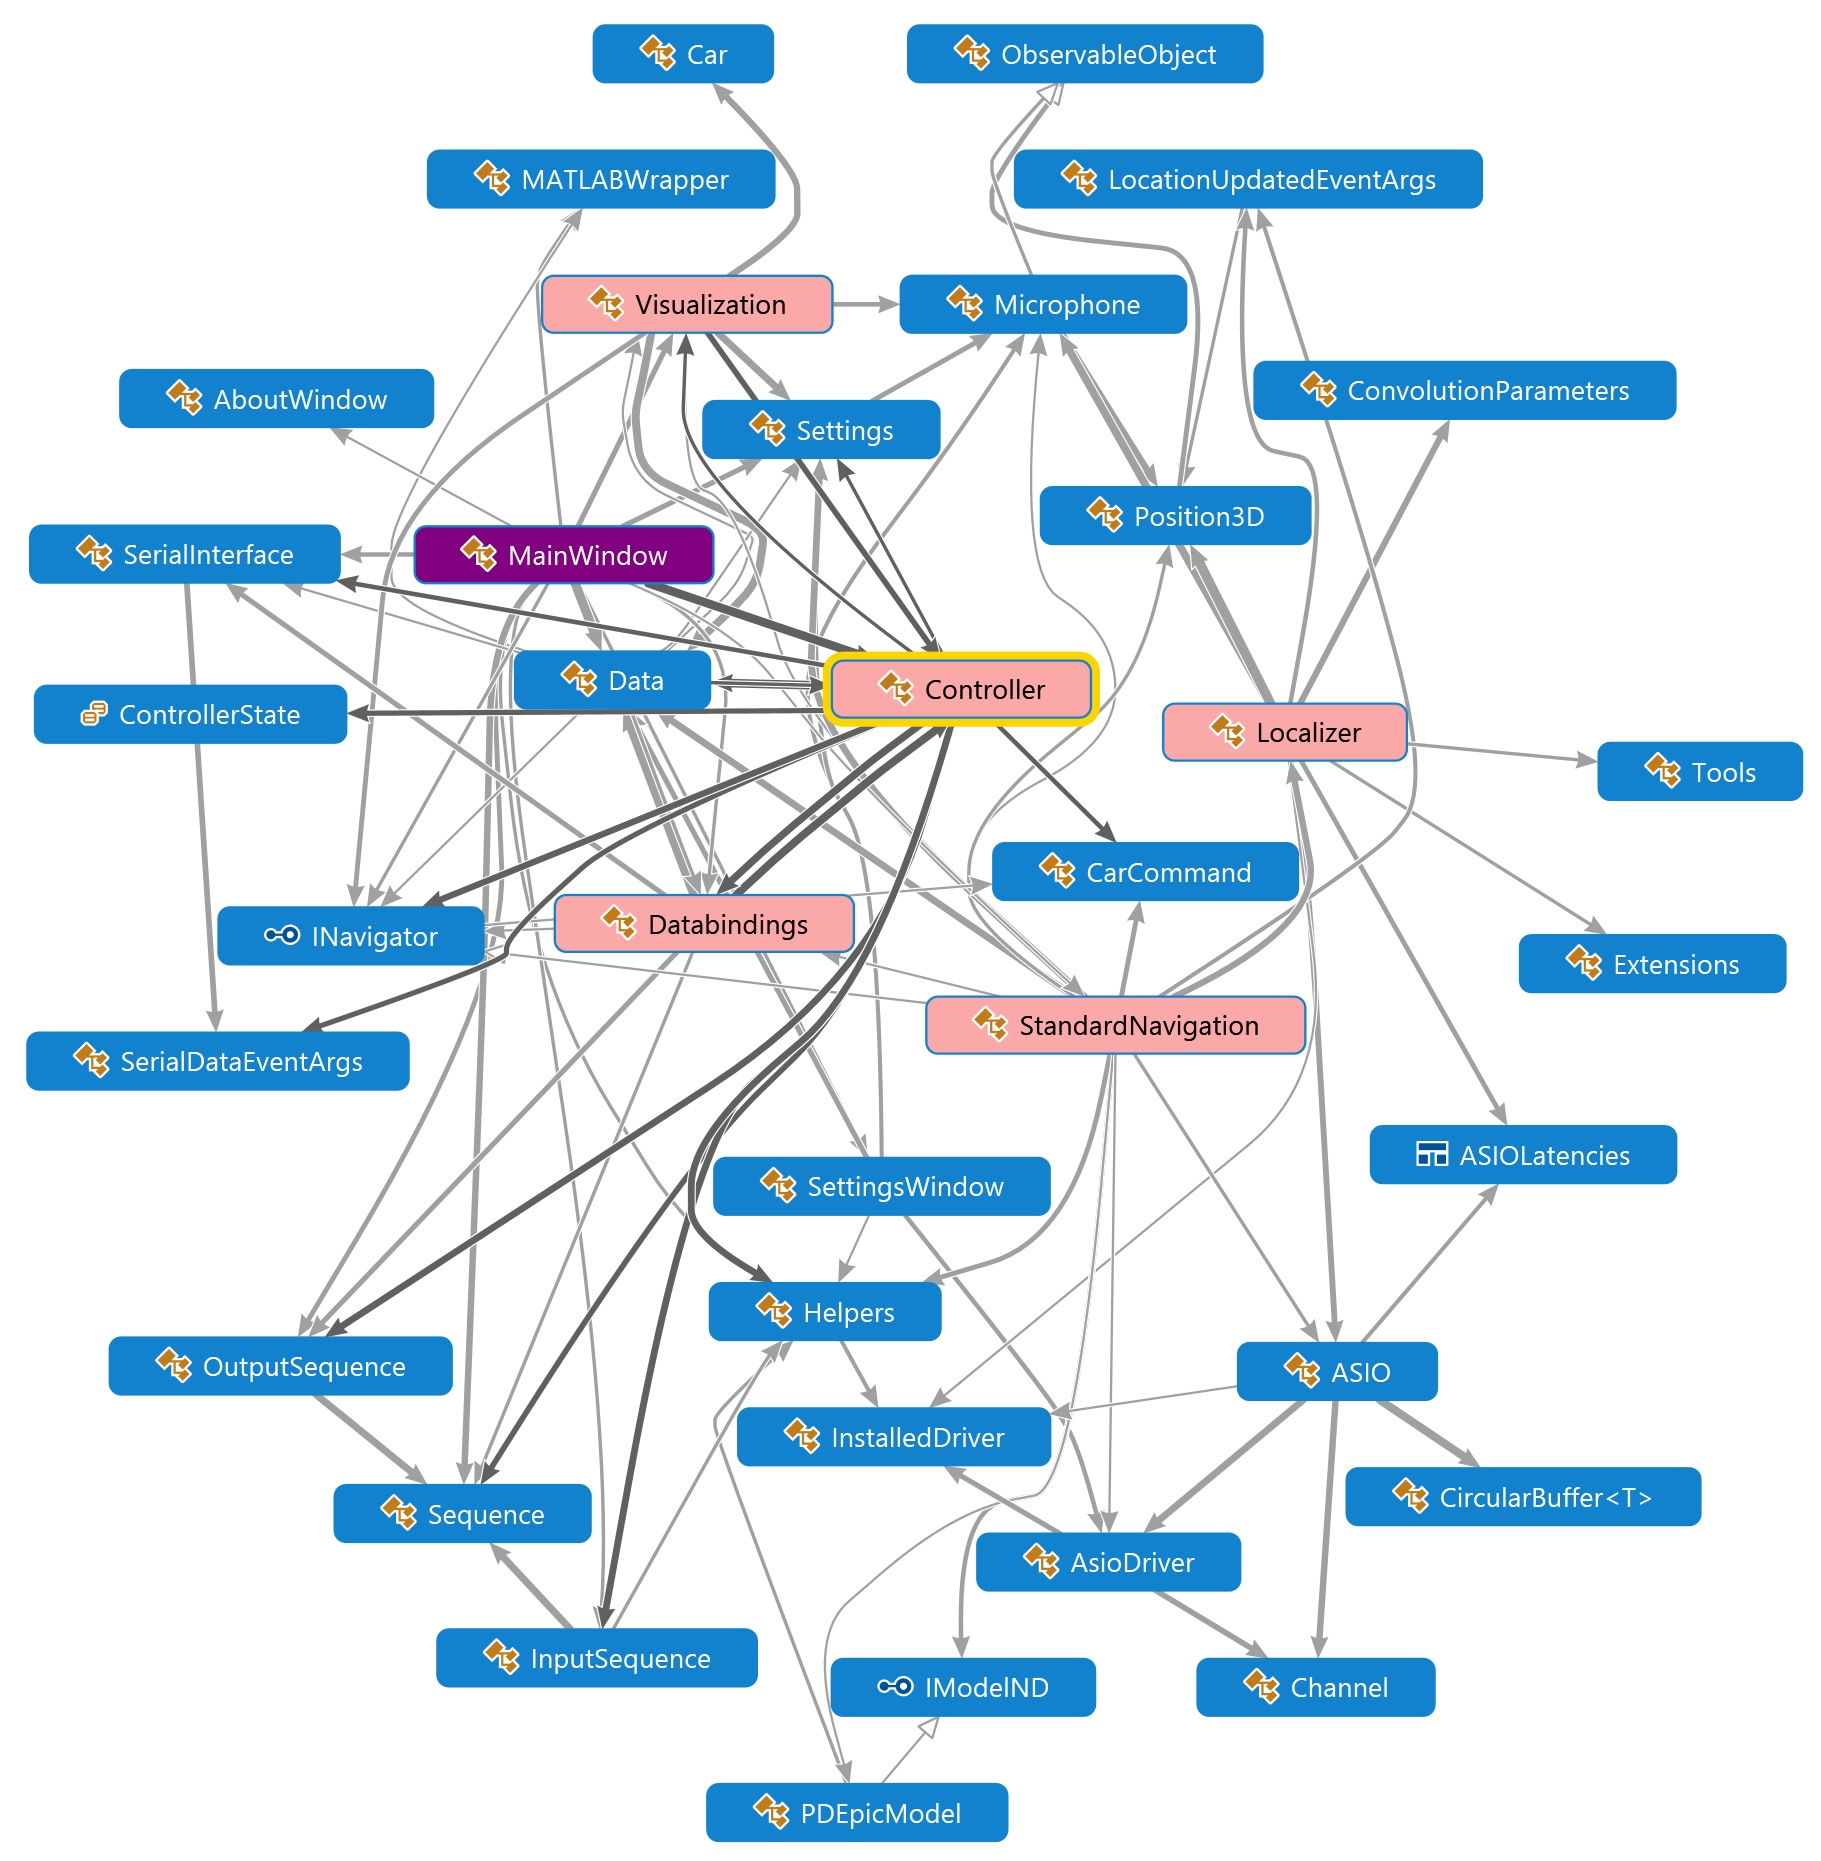
\includegraphics[width=\linewidth]{resources/code-map.jpg}
	\caption{The code map with all the classes that are relevant. Purple means unreferenced classes. Pinks are Hub classes (lots of connections). And the others are normal classes, structs and interfaces.}
	\label{fig:code-map}
\end{figure}

\chapter{Matlab code}
\label{app:code}
\includecode[matlab]{matched-filter.m}{resources/matlab/matched-filter.m}{matched-filter.m}
\newpage
\includecode[matlab]{matched-filter-toep.m}{resources/matlab/matched-filter-toep.m}{matched-filter-toep.m}
\newpage
\includecode[matlab]{report6-2.m}{resources/matlab/report6-2.m}{report6-2.m}
\includecode[matlab]{location.m}{resources/matlab/location.m}{location.m}
\includecode[matlab]{location-errors.m}{resources/matlab/location-errors.m}{location-errors.m}

\chapter{Source}
\label{app:source}
\subimport{}{sourcecode.tex}

\end{appendices}
\end{document}